\PassOptionsToPackage{unicode=true}{hyperref} % options for packages loaded elsewhere
\PassOptionsToPackage{hyphens}{url}
%
\documentclass[ignorenonframetext,]{beamer}
\usepackage{pgfpages}
\setbeamertemplate{caption}[numbered]
\setbeamertemplate{caption label separator}{: }
\setbeamercolor{caption name}{fg=normal text.fg}
\beamertemplatenavigationsymbolsempty
% Prevent slide breaks in the middle of a paragraph:
\widowpenalties 1 10000
\raggedbottom
\setbeamertemplate{part page}{
\centering
\begin{beamercolorbox}[sep=16pt,center]{part title}
  \usebeamerfont{part title}\insertpart\par
\end{beamercolorbox}
}
\setbeamertemplate{section page}{
\centering
\begin{beamercolorbox}[sep=12pt,center]{part title}
  \usebeamerfont{section title}\insertsection\par
\end{beamercolorbox}
}
\setbeamertemplate{subsection page}{
\centering
\begin{beamercolorbox}[sep=8pt,center]{part title}
  \usebeamerfont{subsection title}\insertsubsection\par
\end{beamercolorbox}
}
\AtBeginPart{
  \frame{\partpage}
}
\AtBeginSection{
  \ifbibliography
  \else
    \frame{\sectionpage}
  \fi
}
\AtBeginSubsection{
  \frame{\subsectionpage}
}
\usepackage{lmodern}
\usepackage{amssymb,amsmath}
\usepackage{ifxetex,ifluatex}
\usepackage{fixltx2e} % provides \textsubscript
\ifnum 0\ifxetex 1\fi\ifluatex 1\fi=0 % if pdftex
  \usepackage[T1]{fontenc}
  \usepackage[utf8]{inputenc}
  \usepackage{textcomp} % provides euro and other symbols
\else % if luatex or xelatex
  \usepackage{unicode-math}
  \defaultfontfeatures{Ligatures=TeX,Scale=MatchLowercase}
\fi
\usetheme[]{AnnArbor}
\usecolortheme{dove}
% use upquote if available, for straight quotes in verbatim environments
\IfFileExists{upquote.sty}{\usepackage{upquote}}{}
% use microtype if available
\IfFileExists{microtype.sty}{%
\usepackage[]{microtype}
\UseMicrotypeSet[protrusion]{basicmath} % disable protrusion for tt fonts
}{}
\IfFileExists{parskip.sty}{%
\usepackage{parskip}
}{% else
\setlength{\parindent}{0pt}
\setlength{\parskip}{6pt plus 2pt minus 1pt}
}
\usepackage{hyperref}
\hypersetup{
            pdftitle={STAD29: Statistics for the Life and Social Sciences},
            pdfauthor={Lecture notes},
            pdfborder={0 0 0},
            breaklinks=true}
\urlstyle{same}  % don't use monospace font for urls
\newif\ifbibliography
\usepackage{color}
\usepackage{fancyvrb}
\newcommand{\VerbBar}{|}
\newcommand{\VERB}{\Verb[commandchars=\\\{\}]}
\DefineVerbatimEnvironment{Highlighting}{Verbatim}{commandchars=\\\{\}}
% Add ',fontsize=\small' for more characters per line
\usepackage{framed}
\definecolor{shadecolor}{RGB}{248,248,248}
\newenvironment{Shaded}{\begin{snugshade}}{\end{snugshade}}
\newcommand{\AlertTok}[1]{\textcolor[rgb]{0.94,0.16,0.16}{#1}}
\newcommand{\AnnotationTok}[1]{\textcolor[rgb]{0.56,0.35,0.01}{\textbf{\textit{#1}}}}
\newcommand{\AttributeTok}[1]{\textcolor[rgb]{0.77,0.63,0.00}{#1}}
\newcommand{\BaseNTok}[1]{\textcolor[rgb]{0.00,0.00,0.81}{#1}}
\newcommand{\BuiltInTok}[1]{#1}
\newcommand{\CharTok}[1]{\textcolor[rgb]{0.31,0.60,0.02}{#1}}
\newcommand{\CommentTok}[1]{\textcolor[rgb]{0.56,0.35,0.01}{\textit{#1}}}
\newcommand{\CommentVarTok}[1]{\textcolor[rgb]{0.56,0.35,0.01}{\textbf{\textit{#1}}}}
\newcommand{\ConstantTok}[1]{\textcolor[rgb]{0.00,0.00,0.00}{#1}}
\newcommand{\ControlFlowTok}[1]{\textcolor[rgb]{0.13,0.29,0.53}{\textbf{#1}}}
\newcommand{\DataTypeTok}[1]{\textcolor[rgb]{0.13,0.29,0.53}{#1}}
\newcommand{\DecValTok}[1]{\textcolor[rgb]{0.00,0.00,0.81}{#1}}
\newcommand{\DocumentationTok}[1]{\textcolor[rgb]{0.56,0.35,0.01}{\textbf{\textit{#1}}}}
\newcommand{\ErrorTok}[1]{\textcolor[rgb]{0.64,0.00,0.00}{\textbf{#1}}}
\newcommand{\ExtensionTok}[1]{#1}
\newcommand{\FloatTok}[1]{\textcolor[rgb]{0.00,0.00,0.81}{#1}}
\newcommand{\FunctionTok}[1]{\textcolor[rgb]{0.00,0.00,0.00}{#1}}
\newcommand{\ImportTok}[1]{#1}
\newcommand{\InformationTok}[1]{\textcolor[rgb]{0.56,0.35,0.01}{\textbf{\textit{#1}}}}
\newcommand{\KeywordTok}[1]{\textcolor[rgb]{0.13,0.29,0.53}{\textbf{#1}}}
\newcommand{\NormalTok}[1]{#1}
\newcommand{\OperatorTok}[1]{\textcolor[rgb]{0.81,0.36,0.00}{\textbf{#1}}}
\newcommand{\OtherTok}[1]{\textcolor[rgb]{0.56,0.35,0.01}{#1}}
\newcommand{\PreprocessorTok}[1]{\textcolor[rgb]{0.56,0.35,0.01}{\textit{#1}}}
\newcommand{\RegionMarkerTok}[1]{#1}
\newcommand{\SpecialCharTok}[1]{\textcolor[rgb]{0.00,0.00,0.00}{#1}}
\newcommand{\SpecialStringTok}[1]{\textcolor[rgb]{0.31,0.60,0.02}{#1}}
\newcommand{\StringTok}[1]{\textcolor[rgb]{0.31,0.60,0.02}{#1}}
\newcommand{\VariableTok}[1]{\textcolor[rgb]{0.00,0.00,0.00}{#1}}
\newcommand{\VerbatimStringTok}[1]{\textcolor[rgb]{0.31,0.60,0.02}{#1}}
\newcommand{\WarningTok}[1]{\textcolor[rgb]{0.56,0.35,0.01}{\textbf{\textit{#1}}}}
\usepackage{graphicx,grffile}
\makeatletter
\def\maxwidth{\ifdim\Gin@nat@width>\linewidth\linewidth\else\Gin@nat@width\fi}
\def\maxheight{\ifdim\Gin@nat@height>\textheight\textheight\else\Gin@nat@height\fi}
\makeatother
% Scale images if necessary, so that they will not overflow the page
% margins by default, and it is still possible to overwrite the defaults
% using explicit options in \includegraphics[width, height, ...]{}
\setkeys{Gin}{width=\maxwidth,height=\maxheight,keepaspectratio}
\setlength{\emergencystretch}{3em}  % prevent overfull lines
\providecommand{\tightlist}{%
  \setlength{\itemsep}{0pt}\setlength{\parskip}{0pt}}
\setcounter{secnumdepth}{0}

% set default figure placement to htbp
\makeatletter
\def\fps@figure{htbp}
\makeatother

\usepackage{multicol}

\title{STAD29: Statistics for the Life and Social Sciences}
\author{Lecture notes}
\date{}

\begin{document}
\frame{\titlepage}

\hypertarget{course-outline}{%
\section{Course Outline}\label{course-outline}}

\begin{frame}[fragile]{Course and instructor}
\protect\hypertarget{course-and-instructor}{}

\begin{itemize}
\item
  Lecture: Wednesday 14:00-16:00 in HW 215. Optional computer lab Monday
  16:00-17:00 in BV 498.
\item
  Instructor: Ken Butler
\item
  Office: IC 471.
\item
  E-mail: \texttt{butler@utsc.utoronto.ca}
\item
  Office hours: Monday 11:00-13:00. I am often around otherwise. See if
  I'm in. Or make an appointment. E-mail always good.
\item
  Course website: \href{http://ritsokiguess.site/STAD29/}{link}.
\item
  Using Quercus for assignments/grades only; using website for
  everything else.
\end{itemize}

\end{frame}

\begin{frame}{Texts}
\protect\hypertarget{texts}{}

\begin{itemize}
\item
  There is no official text for this course.
\item
  You may find ``R for Data Science'',
  \href{http://r4ds.had.co.nz/}{\textbf{link}} helpful for R background.
\item
  I will refer frequently to my book of Problems and Solutions in
  Applied Statistics (PASIAS),
  \href{http://ritsokiguess.site/pasias/}{\textbf{link}}.
\item
  Both of these resources are and will remain free.
\end{itemize}

\end{frame}

\begin{frame}{Programs, prerequisites and exclusions}
\protect\hypertarget{programs-prerequisites-and-exclusions}{}

\begin{itemize}
\item
  Prerequisites:
\item
  For undergrads: STAC32. Not negotiable.
\item
  For grad students, a first course in statistics, and some training in
  regression and ANOVA. The less you know, the more you'll have to catch
  up!
\item
  This course is a required part of Applied Statistics minor.
\item
  Exclusions: \textbf{this course is not for Math/Statistics/CS
  majors/minors}. It is for students in other fields who wish to learn
  some more advanced statistical methods. The exclusions in the Calendar
  reflect this.
\item
  If you are in one of those programs, you won't get program credit for
  this course, \textbf{or for any future STA courses you take.}
\end{itemize}

\end{frame}

\begin{frame}{Computing}
\protect\hypertarget{computing}{}

\begin{itemize}
\item
  Computing: big part of the course, \textbf{not} optional. You will
  need to demonstrate that you can use R to analyze data, and can
  critically interpret the output.
\item
  For grad students who have not come through STAC32, I am happy to
  offer extra help to get you up to speed.
\end{itemize}

\end{frame}

\begin{frame}{Assessment 1/2}
\protect\hypertarget{assessment-12}{}

\begin{itemize}
\item
  Grading: (2 hour) midterm, (3 hour) final exam. Assignments most
  weeks, due Tuesday at 11:59pm. Graduate students (STA 1007) also
  required to complete a project using one or more of the techniques
  learned in class, on a dataset from their field of study. Projects due
  on the last day of classes.
\item
  Assessment:

  \begin{tabular}{lcc}
  & STAD29 & STA 1007\\
  Assignments & 20\% & 20\%\\
  Midterm exam & 30\%  & 20\% \\
  Project & - & 20\%\\
  Final exam & 50\% & 40\%
  \end{tabular}
\end{itemize}

\end{frame}

\begin{frame}{Assessment 2/2}
\protect\hypertarget{assessment-22}{}

\begin{itemize}
\item
  Assessments missed \emph{with documentation} will cause a re-weighting
  of other assessments of same type. No make-ups.
\item
  You \textbf{must pass the final exam} to guarantee passing the course.
  If you fail the final exam but would otherwise have passed the course,
  you receive a grade of 45.
\end{itemize}

\end{frame}

\begin{frame}{Plagiarism}
\protect\hypertarget{plagiarism}{}

\begin{itemize}
\item
  \href{http://www.utoronto.ca/academicintegrity/academicoffenses.html}{\textbf{This
  link}} defines academic offences at this university. Read it. You are
  bound by it.
\item
  Plagiarism defined (at the end) as
\end{itemize}

\begin{quote}
The wrongful appropriation and purloining, and publication as one's own,
of the ideas, or the expression of the ideas \ldots{} of another.
\end{quote}

\begin{itemize}
\item
  The code and explanations that you write and hand in must be
  \emph{yours and yours alone}.
\item
  When you hand in work, it is implied that it is \emph{your} work.
  Handing in work, with your name on it, that was actually done by
  someone else is an \emph{academic offence}.
\item
  If I am suspicious that anyone's work is plagiarized, I will take
  action.
\end{itemize}

\end{frame}

\begin{frame}[fragile]{Getting help}
\protect\hypertarget{getting-help}{}

\begin{itemize}
\item
  The English Language Development Centre supports all students in
  developing better Academic English and critical thinking skills needed
  in academic communication. Make use of the personalized support in
  academic writing skills development. Details and sign-up information:
  \href{http://www.utsc.utoronto.ca/eld/}{link}.
\item
  Students with diverse learning styles and needs are welcome in this
  course. In particular, if you have a disability/health consideration
  that may require accommodations, please feel free to approach the
  AccessAbility Services Office as soon as possible. I will work with
  you and AccessAbility Services to ensure you can achieve your learning
  goals in this course. Enquiries are confidential. The UTSC
  AccessAbility Services staff are available by appointment to assess
  specific needs, provide referrals and arrange appropriate
  accommodations: (416) 287-7560 or by e-mail:
  \texttt{ability@utsc.utoronto.ca}.
\end{itemize}

\end{frame}

\begin{frame}{Course material}
\protect\hypertarget{course-material}{}

\begin{itemize}
\tightlist
\item
  Regression-like things

  \begin{itemize}
  \tightlist
  \item
    review of (multiple) regression
  \item
    logistic regression (including multi-category responses)
  \item
    survival analysis
  \end{itemize}
\item
  ANOVA-like things

  \begin{itemize}
  \tightlist
  \item
    more ANOVA
  \item
    multivariate ANOVA
  \item
    repeated measures
  \end{itemize}
\item
  Multivariate methods

  \begin{itemize}
  \tightlist
  \item
    discriminant analysis
  \item
    cluster analysis
  \item
    multidimensional scaling
  \item
    principal components
  \item
    factor analysis
  \end{itemize}
\item
  Miscellanea

  \begin{itemize}
  \tightlist
  \item
    time series
  \item
    multiway frequency tables
  \end{itemize}
\end{itemize}

\end{frame}

\hypertarget{review-of-multiple-regression}{%
\section{Review of (multiple)
regression}\label{review-of-multiple-regression}}

\begin{frame}{Regression}
\protect\hypertarget{regression}{}

\begin{itemize}
\item
  Use regression when one variable is an outcome (\emph{response},
  \(y\)).
\item
  See if/how response depends on other variable(s), \emph{explanatory},
  \(x_1, x_2,\ldots\).
\item
  Can have \emph{one} or \emph{more than one} explanatory variable, but
  always one response.
\item
  Assumes a \emph{straight-line} relationship between response and
  explanatory.
\item
  Ask:

  \begin{itemize}
  \tightlist
  \item
    \emph{is there} a relationship between \(y\) and \(x\)'s, and if so,
    which ones?
  \item
    what does the relationship look like?
  \end{itemize}
\end{itemize}

\end{frame}

\begin{frame}[fragile]{Packages}
\protect\hypertarget{packages}{}

\begin{Shaded}
\begin{Highlighting}[]
\KeywordTok{library}\NormalTok{(MASS) }\CommentTok{# for Box-Cox, later}
\KeywordTok{library}\NormalTok{(tidyverse)}
\KeywordTok{library}\NormalTok{(broom)}
\end{Highlighting}
\end{Shaded}

\end{frame}

\begin{frame}[fragile]{A regression with one \(x\)}
\protect\hypertarget{a-regression-with-one-x}{}

13 children, measure average total sleep time (ATST, mins) and age
(years) for each. See if ATST depends on age. Data in
\texttt{sleep.txt}, ATST then age. Read in data:

\begin{Shaded}
\begin{Highlighting}[]
\NormalTok{my_url <-}\StringTok{ "http://www.utsc.utoronto.ca/~butler/d29/sleep.txt"}
\NormalTok{sleep <-}\StringTok{ }\KeywordTok{read_delim}\NormalTok{(my_url, }\StringTok{" "}\NormalTok{)}
\end{Highlighting}
\end{Shaded}

\begin{verbatim}
## Parsed with column specification:
## cols(
##   atst = col_double(),
##   age = col_double()
## )
\end{verbatim}

\end{frame}

\begin{frame}[fragile]{Check data}
\protect\hypertarget{check-data}{}

\begin{Shaded}
\begin{Highlighting}[]
\KeywordTok{summary}\NormalTok{(sleep)}
\end{Highlighting}
\end{Shaded}

\begin{verbatim}
##       atst            age        
##  Min.   :461.8   Min.   : 4.400  
##  1st Qu.:491.1   1st Qu.: 7.200  
##  Median :528.3   Median : 8.900  
##  Mean   :519.3   Mean   : 9.058  
##  3rd Qu.:532.5   3rd Qu.:11.100  
##  Max.   :586.0   Max.   :14.000
\end{verbatim}

Make scatter plot of ATST (response) vs.~age (explanatory) using code
overleaf:

\end{frame}

\begin{frame}[fragile]{The scatterplot}
\protect\hypertarget{the-scatterplot}{}

\begin{Shaded}
\begin{Highlighting}[]
\KeywordTok{ggplot}\NormalTok{(sleep, }\KeywordTok{aes}\NormalTok{(}\DataTypeTok{x =}\NormalTok{ age, }\DataTypeTok{y =}\NormalTok{ atst)) }\OperatorTok{+}\StringTok{ }\KeywordTok{geom_point}\NormalTok{()}
\end{Highlighting}
\end{Shaded}

\begin{figure}
\centering
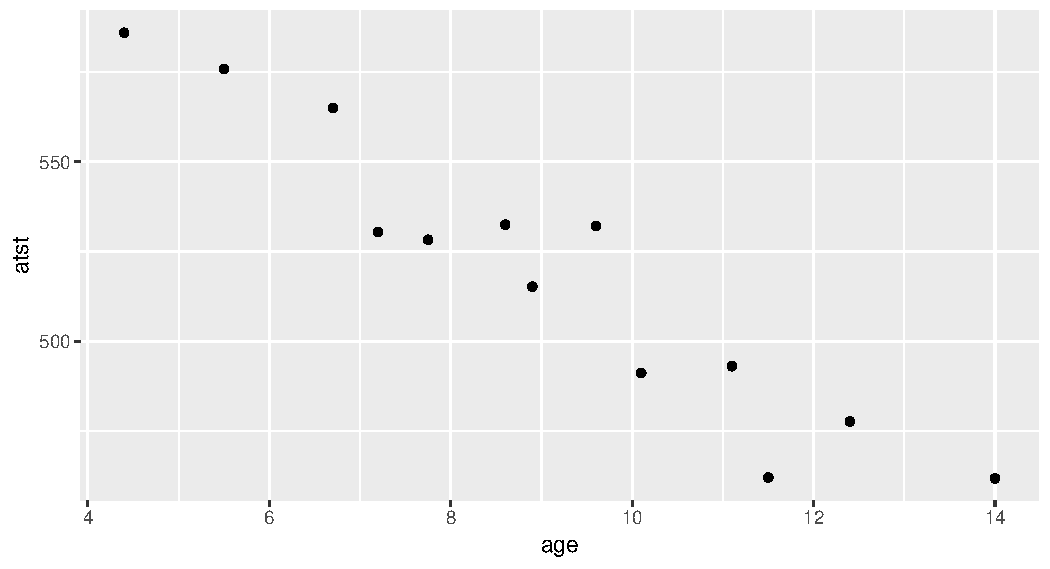
\includegraphics{figure/suggo-1.pdf}
\caption{plot of chunk suggo}
\end{figure}

\end{frame}

\begin{frame}[fragile]{Correlation}
\protect\hypertarget{correlation}{}

\begin{itemize}
\tightlist
\item
  Measures how well a straight line fits the data:
\end{itemize}

\begin{Shaded}
\begin{Highlighting}[]
\KeywordTok{with}\NormalTok{(sleep, }\KeywordTok{cor}\NormalTok{(atst, age))}
\end{Highlighting}
\end{Shaded}

\begin{verbatim}
## [1] -0.9515469
\end{verbatim}

\begin{itemize}
\item
  \(1\) is perfect upward trend, \(-1\) is perfect downward trend, 0 is
  no trend.
\item
  This one close to perfect downward trend.
\item
  Can do correlations of all pairs of variables:
\end{itemize}

\begin{Shaded}
\begin{Highlighting}[]
\KeywordTok{cor}\NormalTok{(sleep)}
\end{Highlighting}
\end{Shaded}

\begin{verbatim}
##            atst        age
## atst  1.0000000 -0.9515469
## age  -0.9515469  1.0000000
\end{verbatim}

\end{frame}

\begin{frame}[fragile]{Lowess curve}
\protect\hypertarget{lowess-curve}{}

\begin{itemize}
\item
  Sometimes nice to guide the eye: is the trend straight, or not?
\item
  Idea: \emph{lowess curve}. ``Locally weighted least squares'', not
  affected by outliers, not constrained to be linear.
\item
  Lowess is a \emph{guide}: even if straight line appropriate, may
  wiggle/bend a little. Looking for \emph{serious} problems with
  linearity.
\item
  Add lowess curve to plot using \texttt{geom\_smooth}:
\end{itemize}

\end{frame}

\begin{frame}[fragile]{Plot with lowess curve}
\protect\hypertarget{plot-with-lowess-curve}{}

\begin{Shaded}
\begin{Highlighting}[]
\KeywordTok{ggplot}\NormalTok{(sleep, }\KeywordTok{aes}\NormalTok{(}\DataTypeTok{x =}\NormalTok{ age, }\DataTypeTok{y =}\NormalTok{ atst)) }\OperatorTok{+}\StringTok{ }\KeywordTok{geom_point}\NormalTok{() }\OperatorTok{+}
\StringTok{  }\KeywordTok{geom_smooth}\NormalTok{()}
\end{Highlighting}
\end{Shaded}

\begin{verbatim}
## `geom_smooth()` using method = 'loess' and formula 'y ~ x'
\end{verbatim}

\begin{figure}
\centering
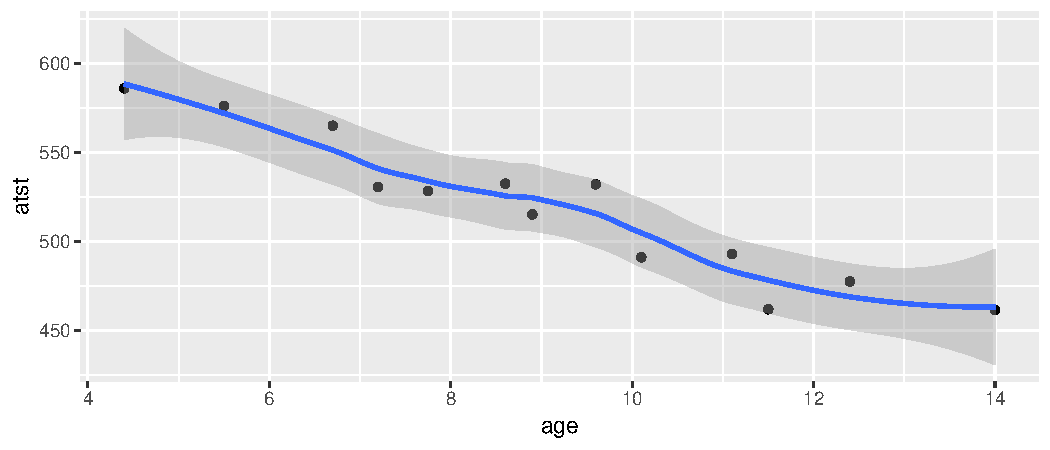
\includegraphics{figure/icko-1.pdf}
\caption{plot of chunk icko}
\end{figure}

\end{frame}

\begin{frame}[fragile]{The regression}
\protect\hypertarget{the-regression}{}

Scatterplot shows no obvious curve, and a pretty clear downward trend.
So we can run the regression:

\begin{Shaded}
\begin{Highlighting}[]
\NormalTok{sleep}\FloatTok{.1}\NormalTok{ <-}\StringTok{ }\KeywordTok{lm}\NormalTok{(atst }\OperatorTok{~}\StringTok{ }\NormalTok{age, }\DataTypeTok{data =}\NormalTok{ sleep)}
\end{Highlighting}
\end{Shaded}

\end{frame}

\begin{frame}[fragile]{The output}
\protect\hypertarget{the-output}{}

\scriptsize

\begin{Shaded}
\begin{Highlighting}[]
\KeywordTok{summary}\NormalTok{(sleep}\FloatTok{.1}\NormalTok{)}
\end{Highlighting}
\end{Shaded}

\begin{verbatim}
## 
## Call:
## lm(formula = atst ~ age, data = sleep)
## 
## Residuals:
##     Min      1Q  Median      3Q     Max 
## -23.011  -9.365   2.372   6.770  20.411 
## 
## Coefficients:
##             Estimate Std. Error t value Pr(>|t|)    
## (Intercept)  646.483     12.918   50.05 2.49e-14 ***
## age          -14.041      1.368  -10.26 5.70e-07 ***
## ---
## Signif. codes:  
## 0 '***' 0.001 '**' 0.01 '*' 0.05 '.' 0.1 ' ' 1
## 
## Residual standard error: 13.15 on 11 degrees of freedom
## Multiple R-squared:  0.9054, Adjusted R-squared:  0.8968 
## F-statistic: 105.3 on 1 and 11 DF,  p-value: 5.7e-07
\end{verbatim}

\normalsize

\end{frame}

\begin{frame}{Conclusions}
\protect\hypertarget{conclusions}{}

\begin{itemize}
\item
  The relationship appears to be a straight line, with a downward trend.
\item
  \(F\)-tests for model as a whole and \(t\)-test for slope (same) both
  confirm this (P-value \(5.7\times 10^{-7}=0.00000057\)).
\item
  Slope is \(-14\), so a 1-year increase in age goes with a 14-minute
  decrease in ATST on average.
\item
  R-squared is correlation squared (when one \(x\) anyway), between 0
  and 1 (1 good, 0 bad).
\item
  Here R-squared is 0.9054, pleasantly high.
\end{itemize}

\end{frame}

\begin{frame}[fragile]{Doing things with the regression output}
\protect\hypertarget{doing-things-with-the-regression-output}{}

\begin{itemize}
\item
  Output from regression (and eg. \(t\)-test) is all right to look at,
  but hard to extract and re-use information from.
\item
  Package \texttt{broom} extracts info from model output in way that can
  be used in pipe (later):
\end{itemize}

\begin{Shaded}
\begin{Highlighting}[]
\KeywordTok{tidy}\NormalTok{(sleep}\FloatTok{.1}\NormalTok{)}
\end{Highlighting}
\end{Shaded}

\begin{verbatim}
## # A tibble: 2 x 5
##   term        estimate std.error statistic  p.value
##   <chr>          <dbl>     <dbl>     <dbl>    <dbl>
## 1 (Intercept)    646.      12.9       50.0 2.49e-14
## 2 age            -14.0      1.37     -10.3 5.70e- 7
\end{verbatim}

\end{frame}

\begin{frame}[fragile]{also one-line summary of model:}
\protect\hypertarget{also-one-line-summary-of-model}{}

\begin{Shaded}
\begin{Highlighting}[]
\KeywordTok{glance}\NormalTok{(sleep}\FloatTok{.1}\NormalTok{)}
\end{Highlighting}
\end{Shaded}

\begin{verbatim}
## # A tibble: 1 x 11
##   r.squared adj.r.squared sigma statistic p.value    df
##       <dbl>         <dbl> <dbl>     <dbl>   <dbl> <int>
## 1     0.905         0.897  13.2      105. 5.70e-7     2
## # … with 5 more variables: logLik <dbl>, AIC <dbl>,
## #   BIC <dbl>, deviance <dbl>, df.residual <int>
\end{verbatim}

\end{frame}

\begin{frame}[fragile]{Broom part 2}
\protect\hypertarget{broom-part-2}{}

\begin{Shaded}
\begin{Highlighting}[]
\NormalTok{sleep}\FloatTok{.1} \OperatorTok\StringTok{ }\KeywordTok{augment}\NormalTok{(sleep) }\OperatorTok\StringTok{ }\KeywordTok{slice}\NormalTok{(}\DecValTok{1}\OperatorTok{:}\DecValTok{8}\NormalTok{)}
\end{Highlighting}
\end{Shaded}

\begin{verbatim}
## # A tibble: 8 x 9
##    atst   age .fitted .se.fit .resid   .hat .sigma .cooksd
##   <dbl> <dbl>   <dbl>   <dbl>  <dbl>  <dbl>  <dbl>   <dbl>
## 1  586    4.4    585.    7.34   1.30 0.312    13.8 0.00320
## 2  462.  14      450.    7.68  11.8  0.341    13.0 0.319  
## 3  491.  10.1    505.    3.92 -13.6  0.0887   13.0 0.0568 
## 4  565    6.7    552.    4.87  12.6  0.137    13.1 0.0844 
## 5  462   11.5    485.    4.95 -23.0  0.141    11.3 0.294  
## 6  532.   9.6    512.    3.72  20.4  0.0801   12.0 0.114  
## 7  478.  12.4    472.    5.85   5.23 0.198    13.7 0.0243 
## 8  515.   8.9    522.    3.65  -6.32 0.0772   13.6 0.0105 
## # … with 1 more variable: .std.resid <dbl>
\end{verbatim}

Useful for plotting residuals against an \(x\)-variable.

\end{frame}

\begin{frame}{CI for mean response and prediction intervals}
\protect\hypertarget{ci-for-mean-response-and-prediction-intervals}{}

Once useful regression exists, use it for prediction:

\begin{itemize}
\item
  To get a single number for prediction at a given \(x\), substitute
  into regression equation, eg. age 10: predicted ATST is
  \(646.48-14.04(10)=506\) minutes.
\item
  To express uncertainty of this prediction:
\item
  \emph{CI for mean response} expresses uncertainty about mean ATST for
  all children aged 10, based on data.
\item
  \emph{Prediction interval} expresses uncertainty about predicted ATST
  for a new child aged 10 whose ATST not known. More uncertain.
\item
  Also do above for a child aged 5.
\end{itemize}

\end{frame}

\begin{frame}[fragile]{Intervals}
\protect\hypertarget{intervals}{}

\begin{itemize}
\tightlist
\item
  Make new data frame with these values for \texttt{age}
\end{itemize}

\begin{Shaded}
\begin{Highlighting}[]
\NormalTok{my.age <-}\StringTok{ }\KeywordTok{c}\NormalTok{(}\DecValTok{10}\NormalTok{, }\DecValTok{5}\NormalTok{)}
\NormalTok{ages.new <-}\StringTok{ }\KeywordTok{tibble}\NormalTok{(}\DataTypeTok{age =}\NormalTok{ my.age)}
\NormalTok{ages.new}
\end{Highlighting}
\end{Shaded}

\begin{verbatim}
## # A tibble: 2 x 1
##     age
##   <dbl>
## 1    10
## 2     5
\end{verbatim}

\begin{itemize}
\tightlist
\item
  Feed into \texttt{predict}:
\end{itemize}

\begin{Shaded}
\begin{Highlighting}[]
\NormalTok{pc <-}\StringTok{ }\KeywordTok{predict}\NormalTok{(sleep}\FloatTok{.1}\NormalTok{, ages.new, }\DataTypeTok{interval =} \StringTok{"c"}\NormalTok{)}
\NormalTok{pp <-}\StringTok{ }\KeywordTok{predict}\NormalTok{(sleep}\FloatTok{.1}\NormalTok{, ages.new, }\DataTypeTok{interval =} \StringTok{"p"}\NormalTok{)}
\end{Highlighting}
\end{Shaded}

\end{frame}

\begin{frame}[fragile]{The intervals}
\protect\hypertarget{the-intervals}{}

Confidence intervals for mean response:

\begin{Shaded}
\begin{Highlighting}[]
\KeywordTok{cbind}\NormalTok{(ages.new, pc)}
\end{Highlighting}
\end{Shaded}

\begin{verbatim}
##   age      fit      lwr      upr
## 1  10 506.0729 497.5574 514.5883
## 2   5 576.2781 561.6578 590.8984
\end{verbatim}

Prediction intervals for new response:

\begin{Shaded}
\begin{Highlighting}[]
\KeywordTok{cbind}\NormalTok{(ages.new, pp)}
\end{Highlighting}
\end{Shaded}

\begin{verbatim}
##   age      fit      lwr      upr
## 1  10 506.0729 475.8982 536.2475
## 2   5 576.2781 543.8474 608.7088
\end{verbatim}

\end{frame}

\begin{frame}[fragile]{Comments}
\protect\hypertarget{comments}{}

\begin{itemize}
\item
  Age 10 closer to centre of data, so intervals are both narrower than
  those for age 5.
\item
  Prediction intervals bigger than CI for mean (additional uncertainty).
\item
  Technical note: output from \texttt{predict} is R \texttt{matrix}, not
  data frame, so Tidyverse \texttt{bind\_cols} does not work. Use base R
  \texttt{cbind}.
\end{itemize}

\end{frame}

\begin{frame}[fragile]{That grey envelope}
\protect\hypertarget{that-grey-envelope}{}

Marks confidence interval for mean for all \(x\):

\begin{Shaded}
\begin{Highlighting}[]
\KeywordTok{ggplot}\NormalTok{(sleep, }\KeywordTok{aes}\NormalTok{(}\DataTypeTok{x =}\NormalTok{ age, }\DataTypeTok{y =}\NormalTok{ atst)) }\OperatorTok{+}\StringTok{ }\KeywordTok{geom_point}\NormalTok{() }\OperatorTok{+}
\StringTok{  }\KeywordTok{geom_smooth}\NormalTok{(}\DataTypeTok{method =} \StringTok{"lm"}\NormalTok{) }\OperatorTok{+}
\StringTok{  }\KeywordTok{scale_y_continuous}\NormalTok{(}\DataTypeTok{breaks =} \KeywordTok{seq}\NormalTok{(}\DecValTok{420}\NormalTok{, }\DecValTok{600}\NormalTok{, }\DecValTok{20}\NormalTok{))}
\end{Highlighting}
\end{Shaded}

\begin{figure}
\centering
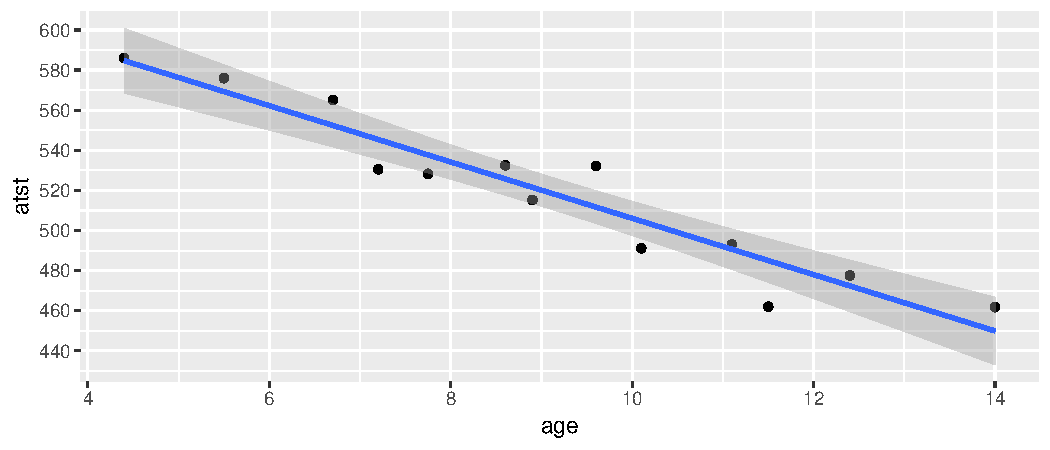
\includegraphics{figure/unnamed-chunk-17-1.pdf}
\caption{plot of chunk unnamed-chunk-17}
\end{figure}

\end{frame}

\begin{frame}{Diagnostics}
\protect\hypertarget{diagnostics}{}

How to tell whether a straight-line regression is appropriate?

\vspace{3ex}

\begin{itemize}
\item
  Before: check scatterplot for straight trend.
\item
  After: plot \emph{residuals} (observed minus predicted response)
  against predicted values. Aim: a plot with no pattern.
\end{itemize}

\end{frame}

\begin{frame}[fragile]{Residual plot}
\protect\hypertarget{residual-plot}{}

Not much pattern here --- regression appropriate.

\begin{Shaded}
\begin{Highlighting}[]
\KeywordTok{ggplot}\NormalTok{(sleep}\FloatTok{.1}\NormalTok{, }\KeywordTok{aes}\NormalTok{(}\DataTypeTok{x =}\NormalTok{ .fitted, }\DataTypeTok{y =}\NormalTok{ .resid)) }\OperatorTok{+}\StringTok{ }\KeywordTok{geom_point}\NormalTok{()}
\end{Highlighting}
\end{Shaded}

\begin{figure}
\centering
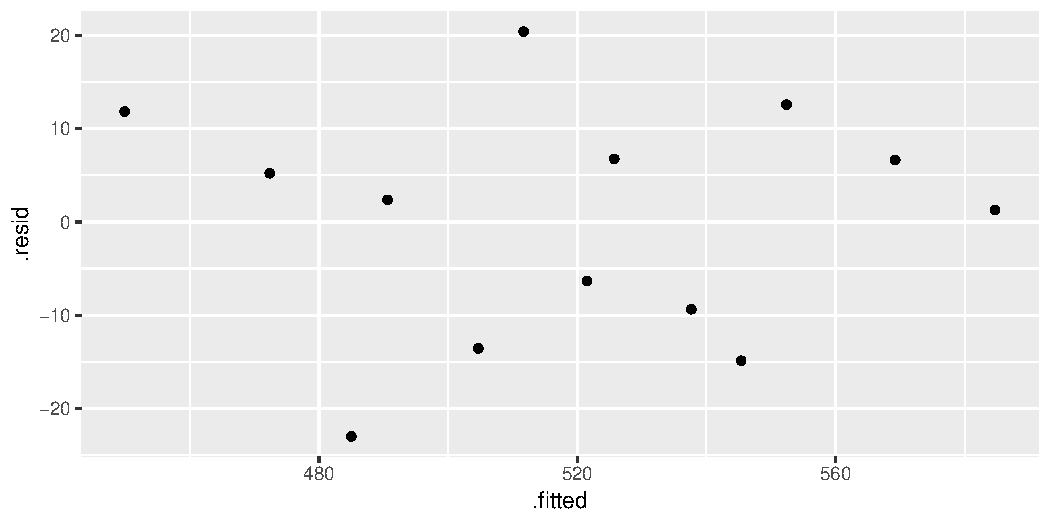
\includegraphics{figure/akjhkadjfhjahnkkk-1.pdf}
\caption{plot of chunk akjhkadjfhjahnkkk}
\end{figure}

\end{frame}

\begin{frame}[fragile]{An inappropriate regression}
\protect\hypertarget{an-inappropriate-regression}{}

Different data:

\begin{Shaded}
\begin{Highlighting}[]
\NormalTok{my_url <-}\StringTok{ "http://www.utsc.utoronto.ca/~butler/d29/curvy.txt"}
\NormalTok{curvy <-}\StringTok{ }\KeywordTok{read_delim}\NormalTok{(my_url, }\StringTok{" "}\NormalTok{)}
\end{Highlighting}
\end{Shaded}

\begin{verbatim}
## Parsed with column specification:
## cols(
##   xx = col_double(),
##   yy = col_double()
## )
\end{verbatim}

\end{frame}

\begin{frame}[fragile]{Scatterplot}
\protect\hypertarget{scatterplot}{}

\begin{Shaded}
\begin{Highlighting}[]
\KeywordTok{ggplot}\NormalTok{(curvy, }\KeywordTok{aes}\NormalTok{(}\DataTypeTok{x =}\NormalTok{ xx, }\DataTypeTok{y =}\NormalTok{ yy)) }\OperatorTok{+}\StringTok{ }\KeywordTok{geom_point}\NormalTok{()}
\end{Highlighting}
\end{Shaded}

\begin{figure}
\centering
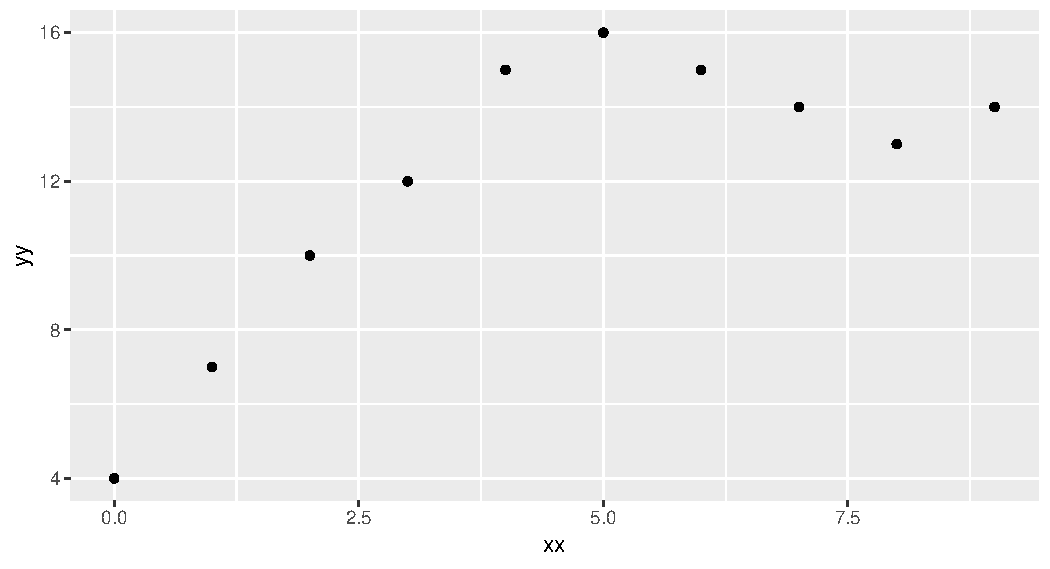
\includegraphics{figure/unnamed-chunk-18-1.pdf}
\caption{plot of chunk unnamed-chunk-18}
\end{figure}

\end{frame}

\begin{frame}[fragile]{Regression line, anyway}
\protect\hypertarget{regression-line-anyway}{}

\scriptsize

\begin{Shaded}
\begin{Highlighting}[]
\NormalTok{curvy}\FloatTok{.1}\NormalTok{ <-}\StringTok{ }\KeywordTok{lm}\NormalTok{(yy }\OperatorTok{~}\StringTok{ }\NormalTok{xx, }\DataTypeTok{data =}\NormalTok{ curvy)}
\KeywordTok{summary}\NormalTok{(curvy}\FloatTok{.1}\NormalTok{)}
\end{Highlighting}
\end{Shaded}

\begin{verbatim}
## 
## Call:
## lm(formula = yy ~ xx, data = curvy)
## 
## Residuals:
##    Min     1Q Median     3Q    Max 
## -3.582 -2.204  0.000  1.514  3.509 
## 
## Coefficients:
##             Estimate Std. Error t value Pr(>|t|)   
## (Intercept)   7.5818     1.5616   4.855  0.00126 **
## xx            0.9818     0.2925   3.356  0.00998 **
## ---
## Signif. codes:  
## 0 '***' 0.001 '**' 0.01 '*' 0.05 '.' 0.1 ' ' 1
## 
## Residual standard error: 2.657 on 8 degrees of freedom
## Multiple R-squared:  0.5848, Adjusted R-squared:  0.5329 
## F-statistic: 11.27 on 1 and 8 DF,  p-value: 0.009984
\end{verbatim}

\normalsize

\end{frame}

\begin{frame}[fragile]{Residual plot}
\protect\hypertarget{residual-plot-1}{}

\begin{Shaded}
\begin{Highlighting}[]
\KeywordTok{ggplot}\NormalTok{(curvy}\FloatTok{.1}\NormalTok{, }\KeywordTok{aes}\NormalTok{(}\DataTypeTok{x =}\NormalTok{ .fitted, }\DataTypeTok{y =}\NormalTok{ .resid)) }\OperatorTok{+}\StringTok{ }\KeywordTok{geom_point}\NormalTok{()}
\end{Highlighting}
\end{Shaded}

\begin{figure}
\centering
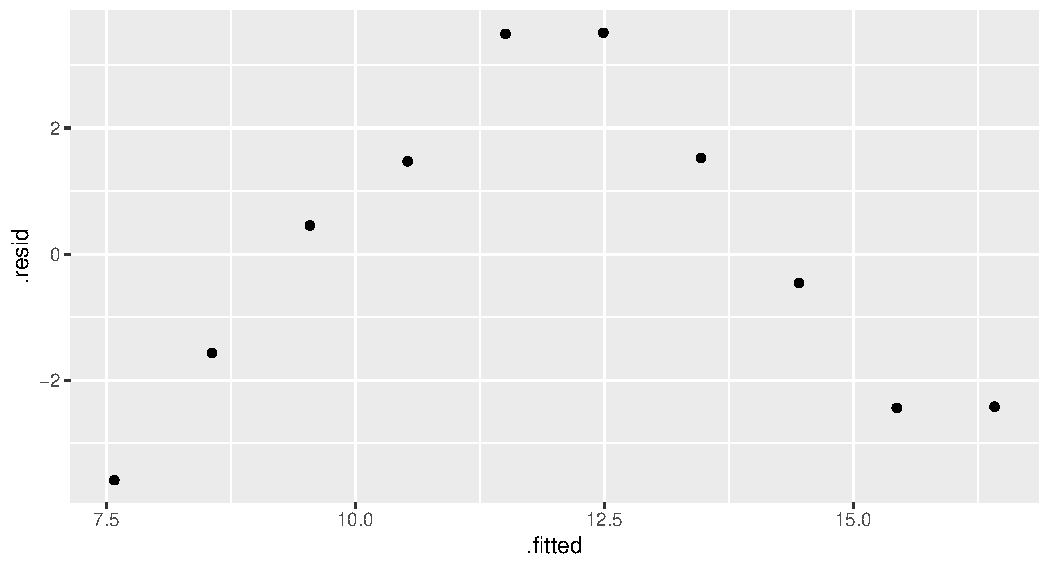
\includegraphics{figure/altoadige-1.pdf}
\caption{plot of chunk altoadige}
\end{figure}

\end{frame}

\begin{frame}[fragile]{No good: fixing it up}
\protect\hypertarget{no-good-fixing-it-up}{}

\begin{itemize}
\item
  Residual plot has \emph{curve}: middle residuals positive, high and
  low ones negative. Bad.
\item
  Fitting a curve would be better. Try this:
\end{itemize}

\begin{Shaded}
\begin{Highlighting}[]
\NormalTok{curvy}\FloatTok{.2}\NormalTok{ <-}\StringTok{ }\KeywordTok{lm}\NormalTok{(yy }\OperatorTok{~}\StringTok{ }\NormalTok{xx }\OperatorTok{+}\StringTok{ }\KeywordTok{I}\NormalTok{(xx}\OperatorTok{^}\DecValTok{2}\NormalTok{), }\DataTypeTok{data =}\NormalTok{ curvy)}
\end{Highlighting}
\end{Shaded}

\begin{itemize}
\item
  Adding \texttt{xx}-squared term, to allow for curve.
\item
  Another way to do same thing: specify how model \emph{changes}:
\end{itemize}

\begin{Shaded}
\begin{Highlighting}[]
\NormalTok{curvy}\FloatTok{.2}\NormalTok{a <-}\StringTok{ }\KeywordTok{update}\NormalTok{(curvy}\FloatTok{.1}\NormalTok{, . }\OperatorTok{~}\StringTok{ }\NormalTok{. }\OperatorTok{+}\StringTok{ }\KeywordTok{I}\NormalTok{(xx}\OperatorTok{^}\DecValTok{2}\NormalTok{))}
\end{Highlighting}
\end{Shaded}

\end{frame}

\begin{frame}[fragile]{Regression 2}
\protect\hypertarget{regression-2}{}

\begin{Shaded}
\begin{Highlighting}[]
\KeywordTok{tidy}\NormalTok{(curvy}\FloatTok{.2}\NormalTok{)}
\end{Highlighting}
\end{Shaded}

\begin{verbatim}
## # A tibble: 3 x 5
##   term        estimate std.error statistic   p.value
##   <chr>          <dbl>     <dbl>     <dbl>     <dbl>
## 1 (Intercept)    3.9      0.773       5.04 0.00149  
## 2 xx             3.74     0.400       9.36 0.0000331
## 3 I(xx^2)       -0.307    0.0428     -7.17 0.000182
\end{verbatim}

\begin{Shaded}
\begin{Highlighting}[]
\KeywordTok{glance}\NormalTok{(curvy}\FloatTok{.2}\NormalTok{) }\CommentTok{#}
\end{Highlighting}
\end{Shaded}

\begin{verbatim}
## # A tibble: 1 x 11
##   r.squared adj.r.squared sigma statistic p.value    df
##       <dbl>         <dbl> <dbl>     <dbl>   <dbl> <int>
## 1     0.950         0.936 0.983      66.8 2.75e-5     3
## # … with 5 more variables: logLik <dbl>, AIC <dbl>,
## #   BIC <dbl>, deviance <dbl>, df.residual <int>
\end{verbatim}

\end{frame}

\begin{frame}[fragile]{Comments}
\protect\hypertarget{comments-1}{}

\begin{itemize}
\item
  \texttt{xx}-squared term definitely significant (P-value 0.000182), so
  need this curve to describe relationship.
\item
  Adding squared term has made R-squared go up from 0.5848 to 0.9502:
  great improvement.
\item
  This is a definite curve!
\end{itemize}

\end{frame}

\begin{frame}[fragile]{The residual plot now}
\protect\hypertarget{the-residual-plot-now}{}

No problems any more:

\begin{Shaded}
\begin{Highlighting}[]
\KeywordTok{ggplot}\NormalTok{(curvy}\FloatTok{.2}\NormalTok{, }\KeywordTok{aes}\NormalTok{(}\DataTypeTok{x =}\NormalTok{ .fitted, }\DataTypeTok{y =}\NormalTok{ .resid)) }\OperatorTok{+}\StringTok{ }\KeywordTok{geom_point}\NormalTok{()}
\end{Highlighting}
\end{Shaded}

\begin{figure}
\centering
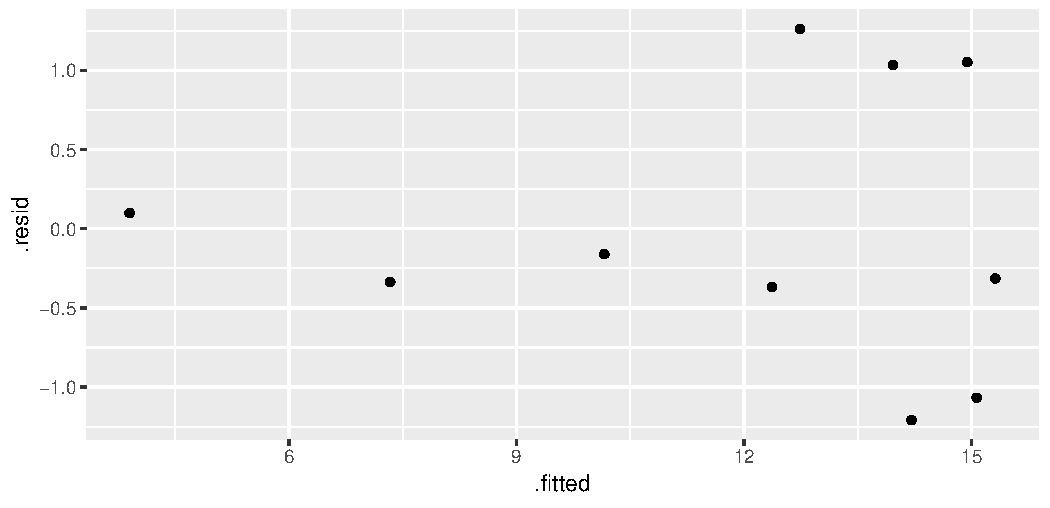
\includegraphics{figure/unnamed-chunk-23-1.pdf}
\caption{plot of chunk unnamed-chunk-23}
\end{figure}

\end{frame}

\begin{frame}{Another way to handle curves}
\protect\hypertarget{another-way-to-handle-curves}{}

\begin{itemize}
\item
  Above, saw that changing \(x\) (adding \(x^2\)) was a way of handling
  curved relationships.
\item
  Another way: change \(y\) (transformation).
\item
  Can guess how to change \(y\), or might be theory:
\item
  example: relationship \(y=ae^{bx}\) (exponential growth):
\item
  take logs to get \(\ln y=\ln a + bx\).
\item
  Taking logs has made relationship linear (\(\ln y\) as response).
\item
  Or, \emph{estimate} transformation, using Box-Cox method.
\end{itemize}

\end{frame}

\begin{frame}[fragile]{Box-Cox}
\protect\hypertarget{box-cox}{}

\begin{itemize}
\item
  Install package \texttt{MASS} via \texttt{install.packages("MASS")}
  (only need to do \emph{once})
\item
  Every R session you want to use something in \texttt{MASS}, type
  \texttt{library(MASS)}
\end{itemize}

\end{frame}

\begin{frame}[fragile]{Some made-up data}
\protect\hypertarget{some-made-up-data}{}

\begin{Shaded}
\begin{Highlighting}[]
\NormalTok{my_url <-}\StringTok{ "http://www.utsc.utoronto.ca/~butler/d29/madeup.csv"}
\NormalTok{madeup <-}\StringTok{ }\KeywordTok{read_csv}\NormalTok{(my_url)}
\NormalTok{madeup}
\end{Highlighting}
\end{Shaded}

\begin{verbatim}
## # A tibble: 8 x 3
##     row     x     y
##   <dbl> <dbl> <dbl>
## 1     1     0  17.9
## 2     2     1  33.6
## 3     3     2  82.7
## 4     4     3  31.2
## 5     5     4 177. 
## 6     6     5 359. 
## 7     7     6 469. 
## 8     8     7 583.
\end{verbatim}

Seems to be faster-than-linear growth, maybe exponential growth.

\end{frame}

\begin{frame}[fragile]{Scatterplot: faster than linear growth}
\protect\hypertarget{scatterplot-faster-than-linear-growth}{}

\begin{Shaded}
\begin{Highlighting}[]
\KeywordTok{ggplot}\NormalTok{(madeup, }\KeywordTok{aes}\NormalTok{(}\DataTypeTok{x =}\NormalTok{ x, }\DataTypeTok{y =}\NormalTok{ y)) }\OperatorTok{+}\StringTok{ }\KeywordTok{geom_point}\NormalTok{() }\OperatorTok{+}
\StringTok{  }\KeywordTok{geom_smooth}\NormalTok{()}
\end{Highlighting}
\end{Shaded}

\begin{verbatim}
## `geom_smooth()` using method = 'loess' and formula 'y ~ x'
\end{verbatim}

\begin{figure}
\centering
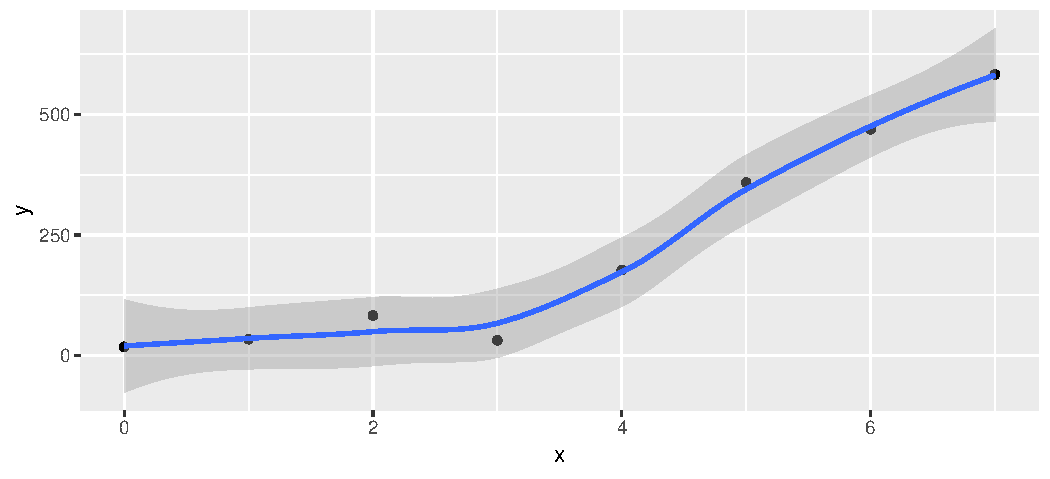
\includegraphics{figure/dsljhsdjlhf-1.pdf}
\caption{plot of chunk dsljhsdjlhf}
\end{figure}

\end{frame}

\begin{frame}[fragile]{Running Box-Cox}
\protect\hypertarget{running-box-cox}{}

\begin{itemize}
\item
  \texttt{library(MASS)} first.
\item
  Feed \texttt{boxcox} a model formula with a squiggle in it, such as
  you would use for \texttt{lm}.
\item
  Output: a graph (next page):
\end{itemize}

\begin{Shaded}
\begin{Highlighting}[]
\KeywordTok{boxcox}\NormalTok{(y }\OperatorTok{~}\StringTok{ }\NormalTok{x, }\DataTypeTok{data =}\NormalTok{ madeup)}
\end{Highlighting}
\end{Shaded}

\end{frame}

\begin{frame}{The Box-Cox output}
\protect\hypertarget{the-box-cox-output}{}

\begin{figure}
\centering
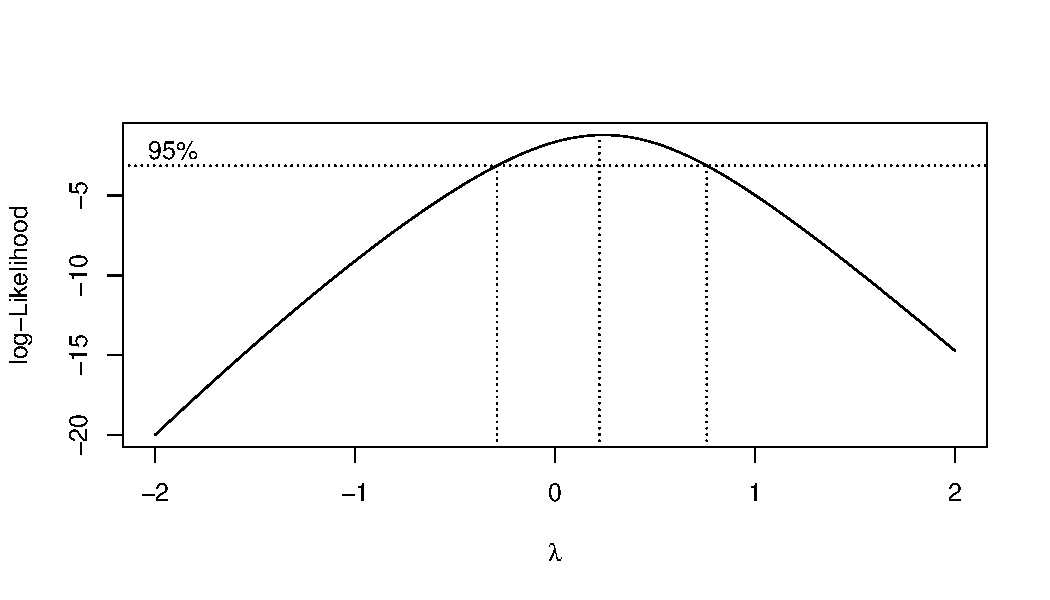
\includegraphics{figure/trento-1.pdf}
\caption{plot of chunk trento}
\end{figure}

\end{frame}

\begin{frame}{Comments}
\protect\hypertarget{comments-2}{}

\begin{itemize}
\item
  \(\lambda\) (lambda) is the power by which you should transform \(y\)
  to get the relationship straight (straighter). Power 0 is ``take
  logs''
\item
  Middle dotted line marks best single value of \(\lambda\) (here about
  0.1).
\item
  Outer dotted lines mark 95\% CI for \(\lambda\), here \(-0.3\) to 0.7,
  approx. (Rather uncertain about best transformation.)
\item
  Any power transformation within the CI supported by data. In this
  case, log (\(\lambda=0\)) and square root (\(\lambda=0.5\)) good, but
  no transformation (\(\lambda=1\)) not.
\item
  Pick a ``round-number'' value of \(\lambda\) like
  \(2,1,0.5,0,-0.5,-1\). Here 0 and 0.5 good values to pick.
\end{itemize}

\end{frame}

\begin{frame}[fragile]{Did transformation straighten things?}
\protect\hypertarget{did-transformation-straighten-things}{}

\begin{itemize}
\tightlist
\item
  Plot transformed \(y\) against \(x\). Here, log:
\end{itemize}

\begin{Shaded}
\begin{Highlighting}[]
\KeywordTok{ggplot}\NormalTok{(madeup, }\KeywordTok{aes}\NormalTok{(}\DataTypeTok{x =}\NormalTok{ x, }\DataTypeTok{y =} \KeywordTok{log}\NormalTok{(y))) }\OperatorTok{+}\StringTok{ }\KeywordTok{geom_point}\NormalTok{() }\OperatorTok{+}
\StringTok{  }\KeywordTok{geom_smooth}\NormalTok{()}
\end{Highlighting}
\end{Shaded}

\begin{figure}
\centering
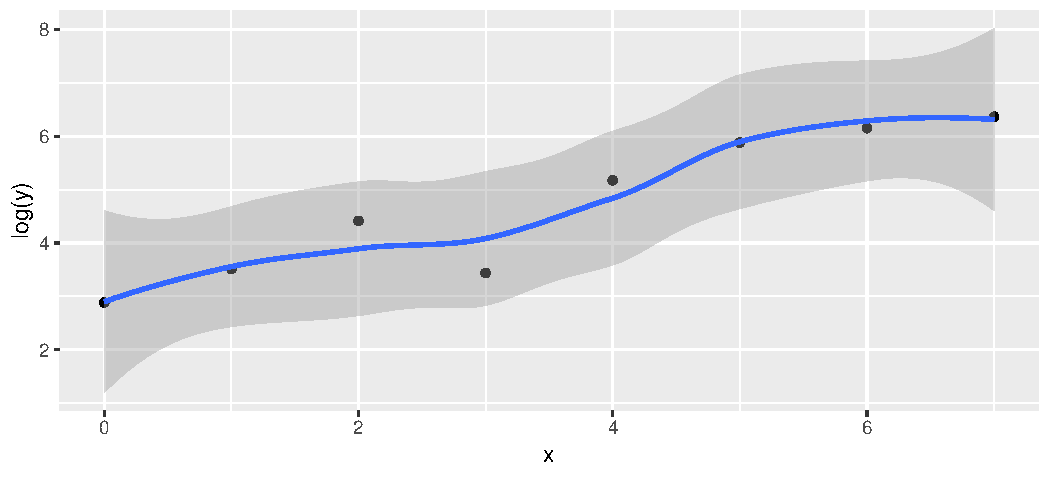
\includegraphics{figure/unnamed-chunk-26-1.pdf}
\caption{plot of chunk unnamed-chunk-26}
\end{figure}

Looks much straighter.

\end{frame}

\begin{frame}[fragile]{Regression with transformed \(y\)}
\protect\hypertarget{regression-with-transformed-y}{}

\footnotesize

\begin{Shaded}
\begin{Highlighting}[]
\NormalTok{madeup}\FloatTok{.1}\NormalTok{ <-}\StringTok{ }\KeywordTok{lm}\NormalTok{(}\KeywordTok{log}\NormalTok{(y) }\OperatorTok{~}\StringTok{ }\NormalTok{x, }\DataTypeTok{data =}\NormalTok{ madeup)}
\KeywordTok{glance}\NormalTok{(madeup}\FloatTok{.1}\NormalTok{)}
\end{Highlighting}
\end{Shaded}

\begin{verbatim}
## # A tibble: 1 x 11
##   r.squared adj.r.squared sigma statistic p.value    df
##       <dbl>         <dbl> <dbl>     <dbl>   <dbl> <int>
## 1     0.883         0.864 0.501      45.3 5.24e-4     2
## # … with 5 more variables: logLik <dbl>, AIC <dbl>,
## #   BIC <dbl>, deviance <dbl>, df.residual <int>
\end{verbatim}

\begin{Shaded}
\begin{Highlighting}[]
\KeywordTok{tidy}\NormalTok{(madeup}\FloatTok{.1}\NormalTok{)}
\end{Highlighting}
\end{Shaded}

\begin{verbatim}
## # A tibble: 2 x 5
##   term        estimate std.error statistic  p.value
##   <chr>          <dbl>     <dbl>     <dbl>    <dbl>
## 1 (Intercept)    2.91     0.323       8.99 0.000106
## 2 x              0.520    0.0773      6.73 0.000524
\end{verbatim}

\normalsize

R-squared now decently high.

\end{frame}

\begin{frame}[fragile]{Multiple regression}
\protect\hypertarget{multiple-regression}{}

\begin{itemize}
\item
  What if more than one \(x\)? Extra issues:

  \begin{itemize}
  \item
    Now one intercept and a slope for each \(x\): how to interpret?
  \item
    Which \(x\)-variables actually help to predict \(y\)?
  \item
    Different interpretations of ``global'' \(F\)-test and individual
    \(t\)-tests.
  \item
    R-squared no longer correlation squared, but still interpreted as
    ``higher better''.
  \item
    In \texttt{lm} line, add extra \(x\)s after
    \texttt{\textasciitilde{}}.
  \item
    Interpretation not so easy (and other problems that can occur).
  \end{itemize}
\end{itemize}

\end{frame}

\begin{frame}[fragile]{Multiple regression example}
\protect\hypertarget{multiple-regression-example}{}

Study of women and visits to health professionals, and how the number of
visits might be related to other variables:

\begin{description}
\item[timedrs:] number of visits to health professionals (over course of study)
\item[phyheal:] number of physical health problems
\item[menheal:] number of mental health problems
\item[stress:] result of questionnaire about number and type of life changes
\end{description}

\texttt{timedrs} response, others explanatory.

\end{frame}

\begin{frame}[fragile]{The data}
\protect\hypertarget{the-data}{}

\begin{Shaded}
\begin{Highlighting}[]
\NormalTok{my_url <-}\StringTok{ }
\StringTok{  "http://www.utsc.utoronto.ca/~butler/d29/regressx.txt"}
\NormalTok{visits <-}\StringTok{ }\KeywordTok{read_delim}\NormalTok{(my_url, }\StringTok{" "}\NormalTok{)}
\end{Highlighting}
\end{Shaded}

\begin{verbatim}
## Parsed with column specification:
## cols(
##   subjno = col_double(),
##   timedrs = col_double(),
##   phyheal = col_double(),
##   menheal = col_double(),
##   stress = col_double()
## )
\end{verbatim}

\end{frame}

\begin{frame}[fragile]{Check data}
\protect\hypertarget{check-data-1}{}

\small

\begin{Shaded}
\begin{Highlighting}[]
\NormalTok{visits}
\end{Highlighting}
\end{Shaded}

\begin{verbatim}
## # A tibble: 465 x 5
##    subjno timedrs phyheal menheal stress
##     <dbl>   <dbl>   <dbl>   <dbl>  <dbl>
##  1      1       1       5       8    265
##  2      2       3       4       6    415
##  3      3       0       3       4     92
##  4      4      13       2       2    241
##  5      5      15       3       6     86
##  6      6       3       5       5    247
##  7      7       2       5       6     13
##  8      8       0       4       5     12
##  9      9       7       5       4    269
## 10     10       4       3       9    391
## # … with 455 more rows
\end{verbatim}

\normalsize

\end{frame}

\begin{frame}[fragile]{Fit multiple regression}
\protect\hypertarget{fit-multiple-regression}{}

\begin{Shaded}
\begin{Highlighting}[]
\NormalTok{visits}\FloatTok{.1}\NormalTok{ <-}\StringTok{ }\KeywordTok{lm}\NormalTok{(timedrs }\OperatorTok{~}\StringTok{ }\NormalTok{phyheal }\OperatorTok{+}\StringTok{ }\NormalTok{menheal }\OperatorTok{+}\StringTok{ }\NormalTok{stress,}
  \DataTypeTok{data =}\NormalTok{ visits)}
\KeywordTok{glance}\NormalTok{(visits}\FloatTok{.1}\NormalTok{)}
\end{Highlighting}
\end{Shaded}

\begin{verbatim}
## # A tibble: 1 x 11
##   r.squared adj.r.squared sigma statistic  p.value    df
##       <dbl>         <dbl> <dbl>     <dbl>    <dbl> <int>
## 1     0.219         0.214  9.71      43.0 1.56e-24     4
## # … with 5 more variables: logLik <dbl>, AIC <dbl>,
## #   BIC <dbl>, deviance <dbl>, df.residual <int>
\end{verbatim}

\end{frame}

\begin{frame}[fragile]{The slopes}
\protect\hypertarget{the-slopes}{}

Model as a whole strongly significant even though R-sq not very big
(lots of data). At least one of the \(x\)'s predicts \texttt{timedrs}.

\begin{Shaded}
\begin{Highlighting}[]
\KeywordTok{tidy}\NormalTok{(visits}\FloatTok{.1}\NormalTok{)}
\end{Highlighting}
\end{Shaded}

\begin{verbatim}
## # A tibble: 4 x 5
##   term        estimate std.error statistic  p.value
##   <chr>          <dbl>     <dbl>     <dbl>    <dbl>
## 1 (Intercept) -3.70      1.12      -3.30   1.06e- 3
## 2 phyheal      1.79      0.221      8.08   5.60e-15
## 3 menheal     -0.00967   0.129     -0.0749 9.40e- 1
## 4 stress       0.0136    0.00361    3.77   1.85e- 4
\end{verbatim}

The physical health and stress variables initely help to predict the
number of visits, but \emph{with those in the model} we don't need
\texttt{menheal}. However, look at prediction of \texttt{timedrs} from
\texttt{menheal} by itself:

\end{frame}

\begin{frame}[fragile]{Just \texttt{menheal}}
\protect\hypertarget{just-menheal}{}

\footnotesize

\begin{Shaded}
\begin{Highlighting}[]
\NormalTok{visits}\FloatTok{.2}\NormalTok{ <-}\StringTok{ }\KeywordTok{lm}\NormalTok{(timedrs }\OperatorTok{~}\StringTok{ }\NormalTok{menheal, }\DataTypeTok{data =}\NormalTok{ visits)}
\KeywordTok{glance}\NormalTok{(visits}\FloatTok{.2}\NormalTok{)}
\end{Highlighting}
\end{Shaded}

\begin{verbatim}
## # A tibble: 1 x 11
##   r.squared adj.r.squared sigma statistic p.value    df
##       <dbl>         <dbl> <dbl>     <dbl>   <dbl> <int>
## 1    0.0653        0.0633  10.6      32.4 2.28e-8     2
## # … with 5 more variables: logLik <dbl>, AIC <dbl>,
## #   BIC <dbl>, deviance <dbl>, df.residual <int>
\end{verbatim}

\begin{Shaded}
\begin{Highlighting}[]
\KeywordTok{tidy}\NormalTok{(visits}\FloatTok{.2}\NormalTok{)}
\end{Highlighting}
\end{Shaded}

\begin{verbatim}
## # A tibble: 2 x 5
##   term        estimate std.error statistic      p.value
##   <chr>          <dbl>     <dbl>     <dbl>        <dbl>
## 1 (Intercept)    3.82      0.870      4.38 0.0000144   
## 2 menheal        0.667     0.117      5.69 0.0000000228
\end{verbatim}

\normalsize

\end{frame}

\begin{frame}[fragile]{\texttt{menheal} by itself}
\protect\hypertarget{menheal-by-itself}{}

\begin{itemize}
\item
  \texttt{menheal} by itself \emph{does} significantly help to predict
  \texttt{timedrs}.
\item
  But the R-sq is much less (6.5\% vs.~22\%).
\item
  So other two variables do a better job of prediction.
\item
  With those variables in the regression (\texttt{phyheal} and
  \texttt{stress}), don't need \texttt{menheal} \emph{as well}.
\end{itemize}

\end{frame}

\begin{frame}[fragile]{Investigating via correlation}
\protect\hypertarget{investigating-via-correlation}{}

Leave out first column (\texttt{subjno}):

\begin{Shaded}
\begin{Highlighting}[]
\NormalTok{visits }\OperatorTok\StringTok{ }\KeywordTok{select}\NormalTok{(}\OperatorTok{-}\NormalTok{subjno) }\OperatorTok\StringTok{ }\KeywordTok{cor}\NormalTok{()}
\end{Highlighting}
\end{Shaded}

\begin{verbatim}
##           timedrs   phyheal   menheal    stress
## timedrs 1.0000000 0.4395293 0.2555703 0.2865951
## phyheal 0.4395293 1.0000000 0.5049464 0.3055517
## menheal 0.2555703 0.5049464 1.0000000 0.3697911
## stress  0.2865951 0.3055517 0.3697911 1.0000000
\end{verbatim}

\begin{itemize}
\item
  \texttt{phyheal} most strongly correlated with \texttt{timedrs}.
\item
  Not much to choose between other two.
\item
  But \texttt{menheal} has higher correlation with \texttt{phyheal}, so
  not as much to \emph{add} to prediction as \texttt{stress}.
\item
  Goes to show things more complicated in multiple regression.
\end{itemize}

\end{frame}

\begin{frame}[fragile]{Residual plot (from \texttt{timedrs} on all)}
\protect\hypertarget{residual-plot-from-timedrs-on-all}{}

\begin{Shaded}
\begin{Highlighting}[]
\KeywordTok{ggplot}\NormalTok{(visits}\FloatTok{.1}\NormalTok{, }\KeywordTok{aes}\NormalTok{(}\DataTypeTok{x =}\NormalTok{ .fitted, }\DataTypeTok{y =}\NormalTok{ .resid)) }\OperatorTok{+}\StringTok{ }\KeywordTok{geom_point}\NormalTok{()}
\end{Highlighting}
\end{Shaded}

\begin{figure}
\centering
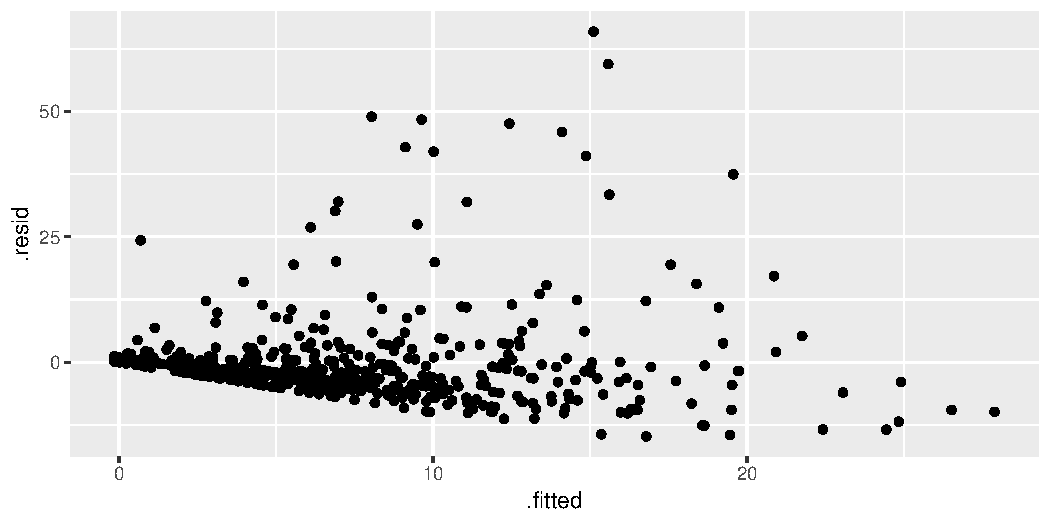
\includegraphics{figure/iffy8-1.pdf}
\caption{plot of chunk iffy8}
\end{figure}

\end{frame}

\begin{frame}{Comment}
\protect\hypertarget{comment}{}

Apparently random. But\ldots

\end{frame}

\begin{frame}[fragile]{Normal quantile plot of residuals}
\protect\hypertarget{normal-quantile-plot-of-residuals}{}

\begin{Shaded}
\begin{Highlighting}[]
\KeywordTok{ggplot}\NormalTok{(visits}\FloatTok{.1}\NormalTok{, }\KeywordTok{aes}\NormalTok{(}\DataTypeTok{sample =}\NormalTok{ .resid)) }\OperatorTok{+}\StringTok{ }\KeywordTok{stat_qq}\NormalTok{() }\OperatorTok{+}\StringTok{ }\KeywordTok{stat_qq_line}\NormalTok{()}
\end{Highlighting}
\end{Shaded}

\begin{figure}
\centering
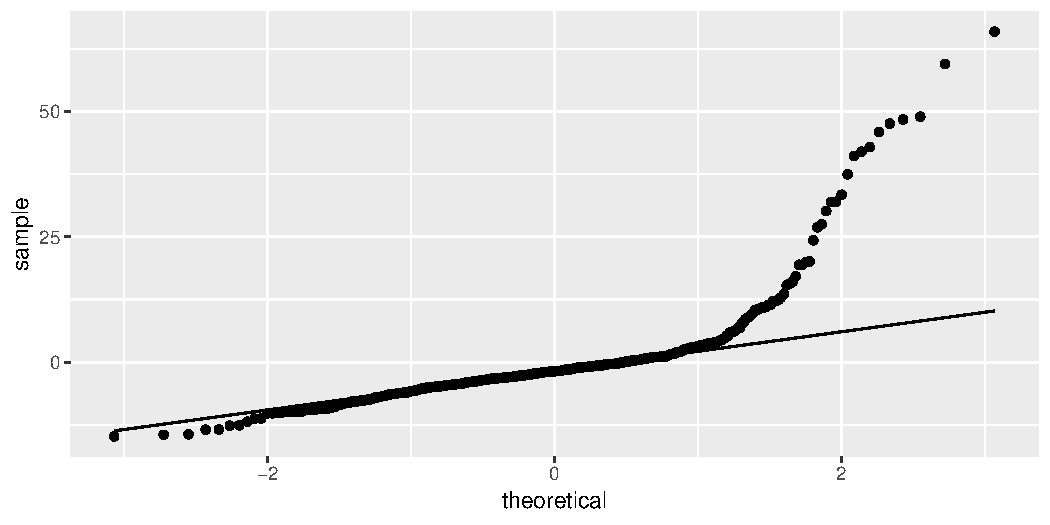
\includegraphics{figure/unnamed-chunk-34-1.pdf}
\caption{plot of chunk unnamed-chunk-34}
\end{figure}

\end{frame}

\begin{frame}[fragile]{Absolute residuals}
\protect\hypertarget{absolute-residuals}{}

Is there trend in \emph{size} of residuals (fan-out)? Plot
\emph{absolute value} of residual against fitted value (graph next
page):

\begin{Shaded}
\begin{Highlighting}[]
\NormalTok{g <-}\StringTok{ }\KeywordTok{ggplot}\NormalTok{(visits}\FloatTok{.1}\NormalTok{, }\KeywordTok{aes}\NormalTok{(}\DataTypeTok{x =}\NormalTok{ .fitted, }\DataTypeTok{y =} \KeywordTok{abs}\NormalTok{(.resid))) }\OperatorTok{+}
\StringTok{  }\KeywordTok{geom_point}\NormalTok{() }\OperatorTok{+}\StringTok{ }\KeywordTok{geom_smooth}\NormalTok{()}
\end{Highlighting}
\end{Shaded}

\end{frame}

\begin{frame}{The plot}
\protect\hypertarget{the-plot}{}

\begin{figure}
\centering
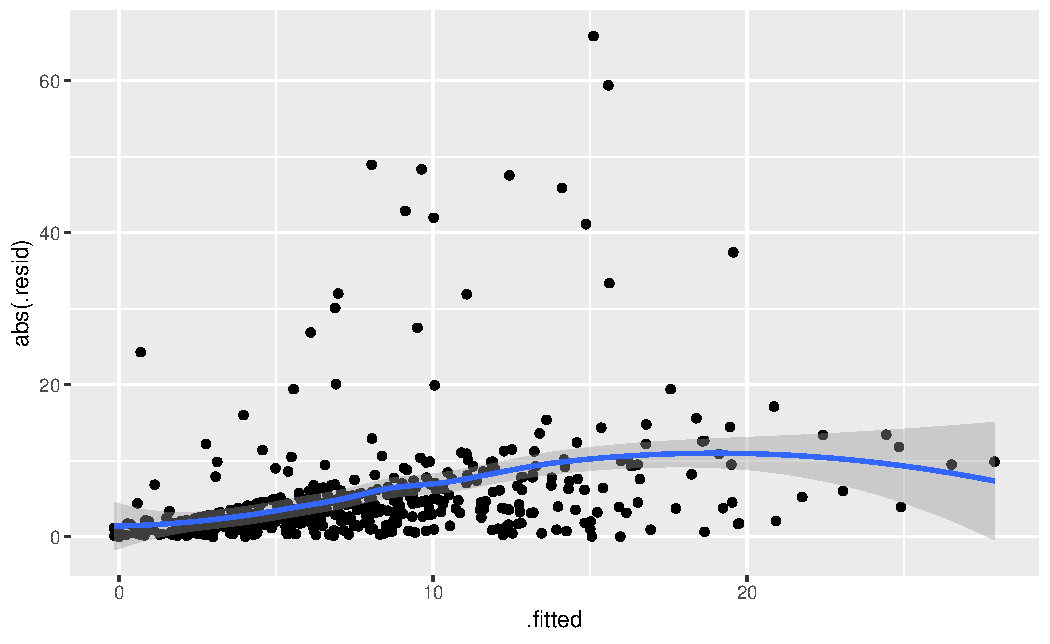
\includegraphics{figure/unnamed-chunk-36-1.pdf}
\caption{plot of chunk unnamed-chunk-36}
\end{figure}

\end{frame}

\begin{frame}[fragile]{Comments}
\protect\hypertarget{comments-3}{}

\begin{itemize}
\item
  On the normal quantile plot:

  \begin{itemize}
  \item
    highest (most positive) residuals are \emph{way} too high
  \item
    distribution of residuals skewed to right (not normal at all)
  \end{itemize}
\item
  On plot of absolute residuals:

  \begin{itemize}
  \item
    size of residuals getting bigger as fitted values increase
  \item
    predictions getting more variable as fitted values increase
  \item
    that is, predictions getting \emph{less accurate} as fitted values
    increase, but predictions should be equally accurate all way along.
  \end{itemize}
\item
  Both indicate problems with regression, of kind that transformation of
  response often fixes: that is, predict \emph{function} of response
  \texttt{timedrs} instead of \texttt{timedrs} itself.
\end{itemize}

\end{frame}

\begin{frame}[fragile]{Box-Cox transformations}
\protect\hypertarget{box-cox-transformations}{}

\begin{itemize}
\item
  Taking log of \texttt{timedrs} and having it work: lucky guess. How to
  find good transformation?
\item
  Box-Cox again.
\item
  Extra problem: some of \texttt{timedrs} values are 0, but Box-Cox
  expects all +. Note response for \texttt{boxcox}:
\end{itemize}

\begin{Shaded}
\begin{Highlighting}[]
\KeywordTok{boxcox}\NormalTok{(timedrs }\OperatorTok{+}\StringTok{ }\DecValTok{1} \OperatorTok{~}\StringTok{ }\NormalTok{phyheal }\OperatorTok{+}\StringTok{ }\NormalTok{menheal }\OperatorTok{+}\StringTok{ }\NormalTok{stress, }\DataTypeTok{data =}\NormalTok{ visits)}
\end{Highlighting}
\end{Shaded}

\end{frame}

\begin{frame}{Try 1}
\protect\hypertarget{try-1}{}

\begin{figure}
\centering
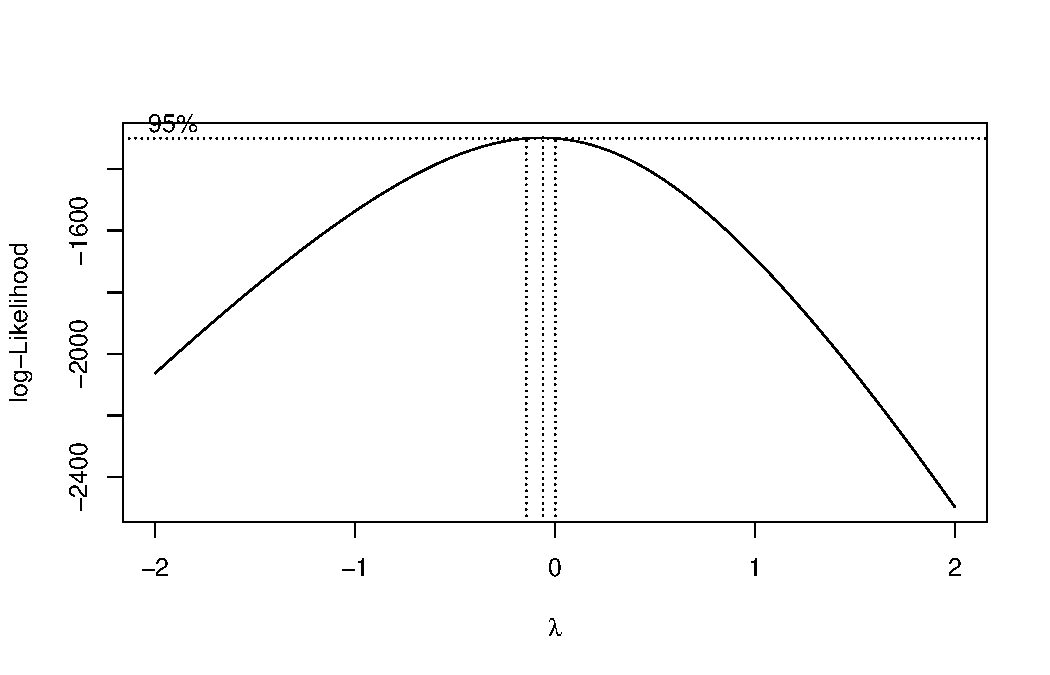
\includegraphics{figure/unnamed-chunk-38-1.pdf}
\caption{plot of chunk unnamed-chunk-38}
\end{figure}

\end{frame}

\begin{frame}[fragile]{Comments on try 1}
\protect\hypertarget{comments-on-try-1}{}

\begin{itemize}
\item
  Best: \(\lambda\) just less than zero.
\item
  Hard to see scale.
\item
  Focus on \(\lambda\) in \((-0.3,0.1)\):
\end{itemize}

\footnotesize

\begin{Shaded}
\begin{Highlighting}[]
\NormalTok{my.lambda <-}\StringTok{ }\KeywordTok{seq}\NormalTok{(}\OperatorTok{-}\FloatTok{0.3}\NormalTok{, }\FloatTok{0.1}\NormalTok{, }\FloatTok{0.01}\NormalTok{)}
\NormalTok{my.lambda}
\end{Highlighting}
\end{Shaded}

\begin{verbatim}
##  [1] -0.30 -0.29 -0.28 -0.27 -0.26 -0.25 -0.24 -0.23 -0.22
## [10] -0.21 -0.20 -0.19 -0.18 -0.17 -0.16 -0.15 -0.14 -0.13
## [19] -0.12 -0.11 -0.10 -0.09 -0.08 -0.07 -0.06 -0.05 -0.04
## [28] -0.03 -0.02 -0.01  0.00  0.01  0.02  0.03  0.04  0.05
## [37]  0.06  0.07  0.08  0.09  0.10
\end{verbatim}

\normalsize

\end{frame}

\begin{frame}[fragile]{Try 2}
\protect\hypertarget{try-2}{}

\begin{Shaded}
\begin{Highlighting}[]
\KeywordTok{boxcox}\NormalTok{(timedrs }\OperatorTok{+}\StringTok{ }\DecValTok{1} \OperatorTok{~}\StringTok{ }\NormalTok{phyheal }\OperatorTok{+}\StringTok{ }\NormalTok{menheal }\OperatorTok{+}\StringTok{ }\NormalTok{stress,}
  \DataTypeTok{lambda =}\NormalTok{ my.lambda,}
  \DataTypeTok{data =}\NormalTok{ visits}
\NormalTok{)}
\end{Highlighting}
\end{Shaded}

\begin{figure}
\centering
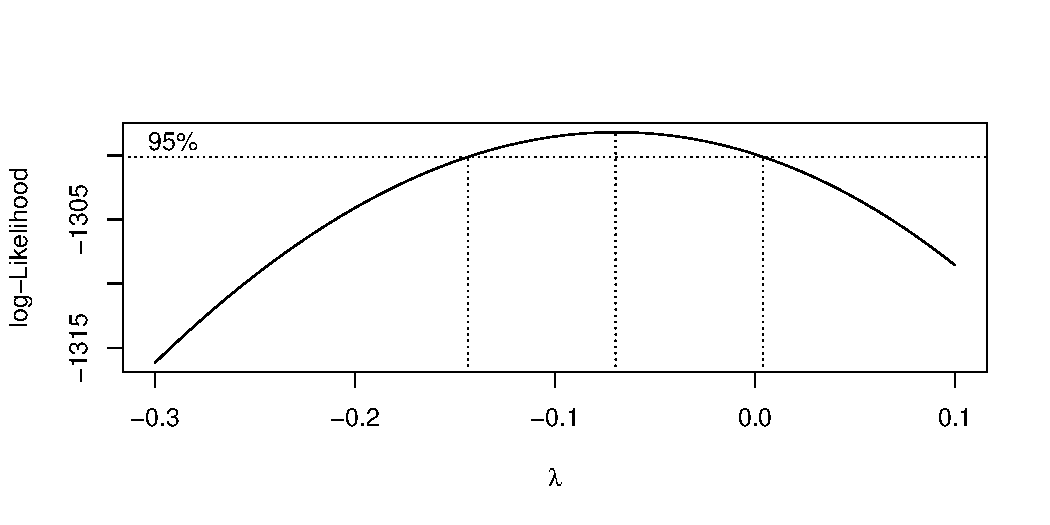
\includegraphics{figure/unnamed-chunk-40-1.pdf}
\caption{plot of chunk unnamed-chunk-40}
\end{figure}

\end{frame}

\begin{frame}{Comments}
\protect\hypertarget{comments-4}{}

\begin{itemize}
\item
  Best: \(\lambda\) just about \(-0.07\).
\item
  CI for \(\lambda\) about \((-0.14,0.01)\).
\item
  Only nearby round number: \(\lambda=0\), log transformation.
\end{itemize}

\end{frame}

\begin{frame}[fragile]{Fixing the problems}
\protect\hypertarget{fixing-the-problems}{}

\begin{itemize}
\item
  Try regression again, with transformed response instead of original
  one.
\item
  Then check residual plot to see that it is OK now.
\end{itemize}

\begin{Shaded}
\begin{Highlighting}[]
\NormalTok{visits}\FloatTok{.3}\NormalTok{ <-}\StringTok{ }\KeywordTok{lm}\NormalTok{(}\KeywordTok{log}\NormalTok{(timedrs }\OperatorTok{+}\StringTok{ }\DecValTok{1}\NormalTok{) }\OperatorTok{~}\StringTok{ }\NormalTok{phyheal }\OperatorTok{+}\StringTok{ }\NormalTok{menheal }\OperatorTok{+}\StringTok{ }\NormalTok{stress,}
  \DataTypeTok{data =}\NormalTok{ visits}
\NormalTok{)}
\end{Highlighting}
\end{Shaded}

\begin{itemize}
\item
  \texttt{timedrs+1} because some \texttt{timedrs} values 0, can't take
  log of 0.
\item
  Won't usually need to worry about this, but when response could be
  zero/negative, fix that before transformation.
\end{itemize}

\end{frame}

\begin{frame}[fragile]{Output}
\protect\hypertarget{output}{}

\scriptsize

\begin{Shaded}
\begin{Highlighting}[]
\KeywordTok{summary}\NormalTok{(visits}\FloatTok{.3}\NormalTok{)}
\end{Highlighting}
\end{Shaded}

\begin{verbatim}
## 
## Call:
## lm(formula = log(timedrs + 1) ~ phyheal + menheal + stress, data = visits)
## 
## Residuals:
##      Min       1Q   Median       3Q      Max 
## -1.95865 -0.44076 -0.02331  0.42304  2.36797 
## 
## Coefficients:
##              Estimate Std. Error t value Pr(>|t|)    
## (Intercept) 0.3903862  0.0882908   4.422 1.22e-05 ***
## phyheal     0.2019361  0.0173624  11.631  < 2e-16 ***
## menheal     0.0071442  0.0101335   0.705    0.481    
## stress      0.0013158  0.0002837   4.638 4.58e-06 ***
## ---
## Signif. codes:  
## 0 '***' 0.001 '**' 0.01 '*' 0.05 '.' 0.1 ' ' 1
## 
## Residual standard error: 0.7625 on 461 degrees of freedom
## Multiple R-squared:  0.3682, Adjusted R-squared:  0.3641 
## F-statistic: 89.56 on 3 and 461 DF,  p-value: < 2.2e-16
\end{verbatim}

\normalsize

\end{frame}

\begin{frame}[fragile]{Comments}
\protect\hypertarget{comments-5}{}

\begin{itemize}
\item
  Model as a whole strongly significant again
\item
  R-sq higher than before (37\% vs.~22\%) suggesting things more linear
  now
\item
  Same conclusion re \texttt{menheal}: can take out of regression.
\item
  Should look at residual plots (next pages). Have we fixed problems?
\end{itemize}

\end{frame}

\begin{frame}[fragile]{Residuals against fitted values}
\protect\hypertarget{residuals-against-fitted-values}{}

\begin{Shaded}
\begin{Highlighting}[]
\KeywordTok{ggplot}\NormalTok{(visits}\FloatTok{.3}\NormalTok{, }\KeywordTok{aes}\NormalTok{(}\DataTypeTok{x =}\NormalTok{ .fitted, }\DataTypeTok{y =}\NormalTok{ .resid)) }\OperatorTok{+}
\StringTok{  }\KeywordTok{geom_point}\NormalTok{()}
\end{Highlighting}
\end{Shaded}

\begin{figure}
\centering
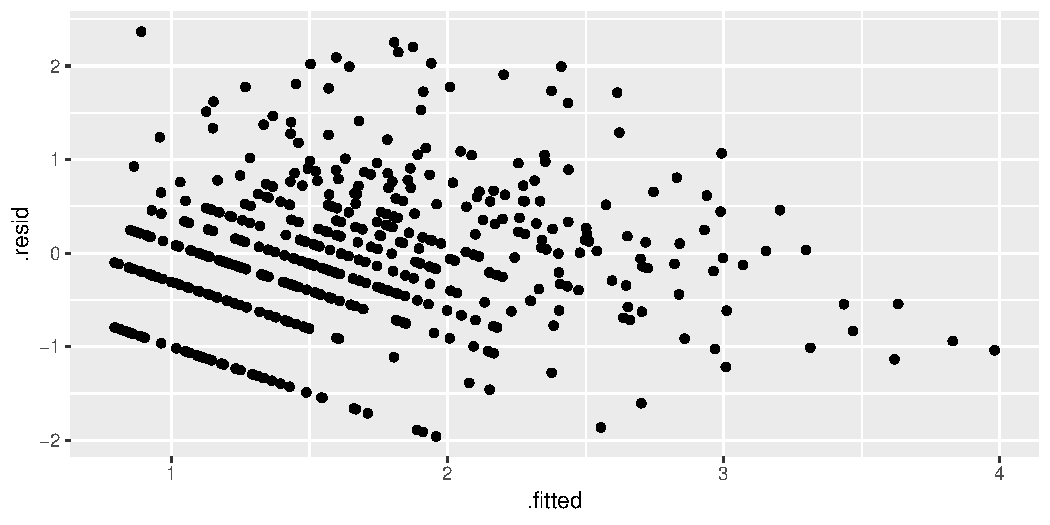
\includegraphics{figure/unnamed-chunk-43-1.pdf}
\caption{plot of chunk unnamed-chunk-43}
\end{figure}

\end{frame}

\begin{frame}[fragile]{Normal quantile plot of residuals}
\protect\hypertarget{normal-quantile-plot-of-residuals-1}{}

\begin{Shaded}
\begin{Highlighting}[]
\KeywordTok{ggplot}\NormalTok{(visits}\FloatTok{.3}\NormalTok{, }\KeywordTok{aes}\NormalTok{(}\DataTypeTok{sample =}\NormalTok{ .resid)) }\OperatorTok{+}\StringTok{ }\KeywordTok{stat_qq}\NormalTok{() }\OperatorTok{+}\StringTok{ }\KeywordTok{stat_qq_line}\NormalTok{()}
\end{Highlighting}
\end{Shaded}

\begin{figure}
\centering
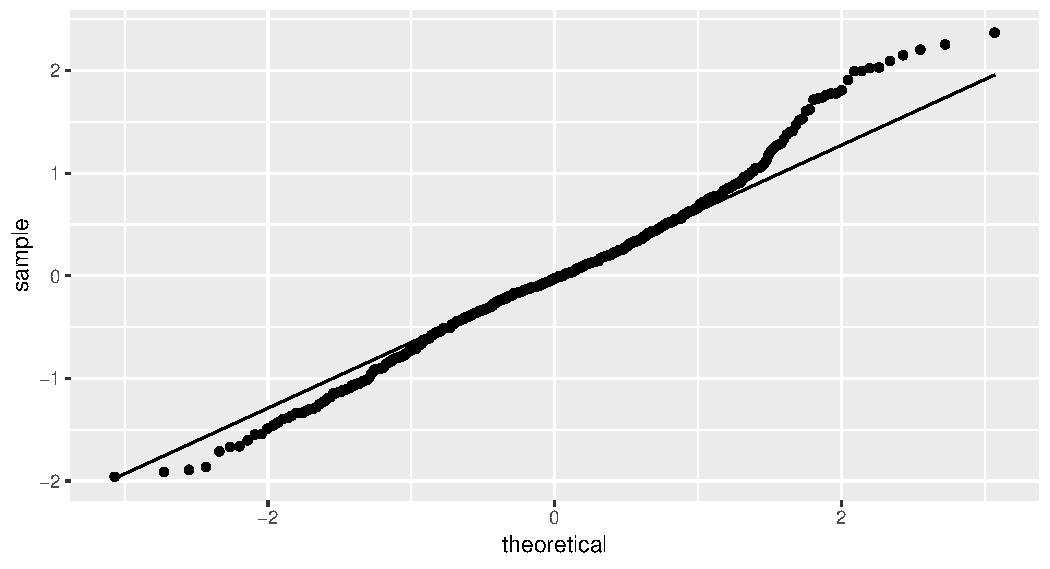
\includegraphics{figure/unnamed-chunk-44-1.pdf}
\caption{plot of chunk unnamed-chunk-44}
\end{figure}

\end{frame}

\begin{frame}[fragile]{Absolute residuals against fitted}
\protect\hypertarget{absolute-residuals-against-fitted}{}

\begin{Shaded}
\begin{Highlighting}[]
\KeywordTok{ggplot}\NormalTok{(visits}\FloatTok{.3}\NormalTok{, }\KeywordTok{aes}\NormalTok{(}\DataTypeTok{x =}\NormalTok{ .fitted, }\DataTypeTok{y =} \KeywordTok{abs}\NormalTok{(.resid))) }\OperatorTok{+}
\StringTok{  }\KeywordTok{geom_point}\NormalTok{() }\OperatorTok{+}\StringTok{ }\KeywordTok{geom_smooth}\NormalTok{()}
\end{Highlighting}
\end{Shaded}

\begin{figure}
\centering
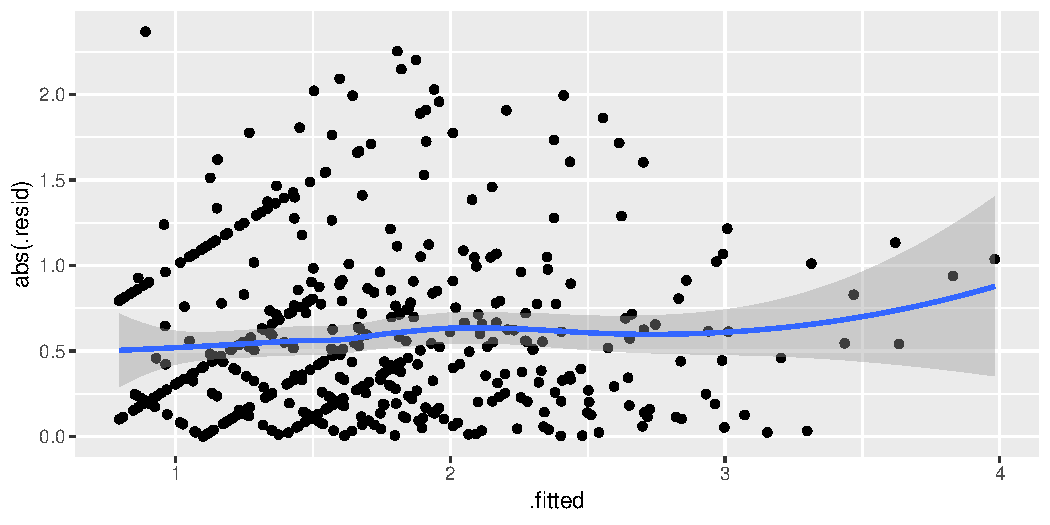
\includegraphics{figure/unnamed-chunk-45-1.pdf}
\caption{plot of chunk unnamed-chunk-45}
\end{figure}

\end{frame}

\begin{frame}{Comments}
\protect\hypertarget{comments-6}{}

\begin{itemize}
\item
  Residuals vs.~fitted looks a lot more random.
\item
  Normal quantile plot looks a lot more normal (though still a little
  right-skewness)
\item
  Absolute residuals: not so much trend (though still some).
\item
  Not perfect, but much improved.
\end{itemize}

\end{frame}

\begin{frame}[fragile]{Testing more than one \(x\) at once}
\protect\hypertarget{testing-more-than-one-x-at-once}{}

\begin{itemize}
\tightlist
\item
  The \(t\)-tests test only whether one variable could be taken out of
  the regression you're looking at.
\item
  To test significance of more than one variable at once, fit model with
  and without variables

  \begin{itemize}
  \tightlist
  \item
    then use \texttt{anova} to compare fit of models:
  \end{itemize}
\end{itemize}

\begin{Shaded}
\begin{Highlighting}[]
\NormalTok{visits}\FloatTok{.5}\NormalTok{ <-}\StringTok{ }\KeywordTok{lm}\NormalTok{(}\KeywordTok{log}\NormalTok{(timedrs }\OperatorTok{+}\StringTok{ }\DecValTok{1}\NormalTok{) }\OperatorTok{~}\StringTok{ }\NormalTok{phyheal }\OperatorTok{+}\StringTok{ }\NormalTok{menheal }\OperatorTok{+}\StringTok{ }\NormalTok{stress, }
               \DataTypeTok{data =}\NormalTok{ visits)}
\NormalTok{visits}\FloatTok{.6}\NormalTok{ <-}\StringTok{ }\KeywordTok{lm}\NormalTok{(}\KeywordTok{log}\NormalTok{(timedrs }\OperatorTok{+}\StringTok{ }\DecValTok{1}\NormalTok{) }\OperatorTok{~}\StringTok{ }\NormalTok{stress, }\DataTypeTok{data =}\NormalTok{ visits)}
\end{Highlighting}
\end{Shaded}

\end{frame}

\begin{frame}[fragile]{Results of tests}
\protect\hypertarget{results-of-tests}{}

\begin{Shaded}
\begin{Highlighting}[]
\KeywordTok{anova}\NormalTok{(visits}\FloatTok{.6}\NormalTok{, visits}\FloatTok{.5}\NormalTok{)}
\end{Highlighting}
\end{Shaded}

\begin{verbatim}
## Analysis of Variance Table
## 
## Model 1: log(timedrs + 1) ~ stress
## Model 2: log(timedrs + 1) ~ phyheal + menheal + stress
##   Res.Df    RSS Df Sum of Sq      F    Pr(>F)    
## 1    463 371.47                                  
## 2    461 268.01  2    103.46 88.984 < 2.2e-16 ***
## ---
## Signif. codes:  
## 0 '***' 0.001 '**' 0.01 '*' 0.05 '.' 0.1 ' ' 1
\end{verbatim}

\begin{itemize}
\item
  Models don't fit equally well, so bigger one fits better.
\item
  Or ``taking both variables out makes the fit worse, so don't do it''.
\item
  Taking out those \(x\)'s is a mistake. Or putting them in is a good
  idea.
\end{itemize}

\end{frame}

\begin{frame}[fragile]{The punting data}
\protect\hypertarget{the-punting-data}{}

Data set \texttt{punting.txt} contains 4 variables for 13 right-footed
football kickers (punters): left leg and right leg strength (lbs),
distance punted (ft), another variable called ``fred''. Predict punting
distance from other variables:

\scriptsize

\begin{verbatim}
left            right               punt         fred
170               170                162.50       171 
130               140                144.0        136   
170               180                174.50       174 
160               160                163.50       161 
150               170                192.0        159 
150               150                171.75       151 
180               170                162.0        174 
110               110                104.83       111 
110               120                105.67       114 
120               130                117.58       126 
140               120                140.25       129  
130               140                150.17       136 
150               160                165.17       154 
\end{verbatim}

\normalsize

\end{frame}

\begin{frame}[fragile]{Reading in}
\protect\hypertarget{reading-in}{}

\begin{itemize}
\tightlist
\item
  Separated by \emph{multiple spaces} with \emph{columns lined up}:
\end{itemize}

\begin{Shaded}
\begin{Highlighting}[]
\NormalTok{my_url <-}\StringTok{ "http://www.utsc.utoronto.ca/~butler/d29/punting.txt"}
\NormalTok{punting <-}\StringTok{ }\KeywordTok{read_table}\NormalTok{(my_url)}
\end{Highlighting}
\end{Shaded}

\begin{verbatim}
## Parsed with column specification:
## cols(
##   left = col_double(),
##   right = col_double(),
##   punt = col_double(),
##   fred = col_double()
## )
\end{verbatim}

\end{frame}

\begin{frame}[fragile]{The data}
\protect\hypertarget{the-data-1}{}

\small

\begin{Shaded}
\begin{Highlighting}[]
\NormalTok{punting}
\end{Highlighting}
\end{Shaded}

\begin{verbatim}
## # A tibble: 13 x 4
##     left right  punt  fred
##    <dbl> <dbl> <dbl> <dbl>
##  1   170   170  162.   171
##  2   130   140  144    136
##  3   170   180  174.   174
##  4   160   160  164.   161
##  5   150   170  192    159
##  6   150   150  172.   151
##  7   180   170  162    174
##  8   110   110  105.   111
##  9   110   120  106.   114
## 10   120   130  118.   126
## 11   140   120  140.   129
## 12   130   140  150.   136
## 13   150   160  165.   154
\end{verbatim}

\normalsize

\end{frame}

\begin{frame}[fragile]{Regression and output}
\protect\hypertarget{regression-and-output}{}

\small

\begin{Shaded}
\begin{Highlighting}[]
\NormalTok{punting}\FloatTok{.1}\NormalTok{ <-}\StringTok{ }\KeywordTok{lm}\NormalTok{(punt }\OperatorTok{~}\StringTok{ }\NormalTok{left }\OperatorTok{+}\StringTok{ }\NormalTok{right }\OperatorTok{+}\StringTok{ }\NormalTok{fred, }\DataTypeTok{data =}\NormalTok{ punting)}
\KeywordTok{glance}\NormalTok{(punting}\FloatTok{.1}\NormalTok{)}
\end{Highlighting}
\end{Shaded}

\begin{verbatim}
## # A tibble: 1 x 11
##   r.squared adj.r.squared sigma statistic p.value    df
##       <dbl>         <dbl> <dbl>     <dbl>   <dbl> <int>
## 1     0.778         0.704  14.7      10.5 0.00267     4
## # … with 5 more variables: logLik <dbl>, AIC <dbl>,
## #   BIC <dbl>, deviance <dbl>, df.residual <int>
\end{verbatim}

\begin{Shaded}
\begin{Highlighting}[]
\KeywordTok{tidy}\NormalTok{(punting}\FloatTok{.1}\NormalTok{)}
\end{Highlighting}
\end{Shaded}

\begin{verbatim}
## # A tibble: 4 x 5
##   term        estimate std.error statistic p.value
##   <chr>          <dbl>     <dbl>     <dbl>   <dbl>
## 1 (Intercept)   -4.69      29.1    -0.161    0.876
## 2 left           0.268      2.11    0.127    0.902
## 3 right          1.05       2.15    0.490    0.636
## 4 fred          -0.267      4.23   -0.0632   0.951
\end{verbatim}

\normalsize

\end{frame}

\begin{frame}{Comments}
\protect\hypertarget{comments-7}{}

\begin{itemize}
\item
  Overall regression strongly significant, R-sq high.
\item
  None of the \(x\)'s significant! Why?
\item
  \(t\)-tests only say that you could take any one of the \(x\)'s out
  without damaging the fit; doesn't matter which one.
\item
  Explanation: look at \emph{correlations}.
\end{itemize}

\end{frame}

\begin{frame}[fragile]{The correlations}
\protect\hypertarget{the-correlations}{}

\begin{Shaded}
\begin{Highlighting}[]
\KeywordTok{cor}\NormalTok{(punting)}
\end{Highlighting}
\end{Shaded}

\begin{verbatim}
##            left     right      punt      fred
## left  1.0000000 0.8957224 0.8117368 0.9722632
## right 0.8957224 1.0000000 0.8805469 0.9728784
## punt  0.8117368 0.8805469 1.0000000 0.8679507
## fred  0.9722632 0.9728784 0.8679507 1.0000000
\end{verbatim}

\begin{itemize}
\item
  \emph{All} correlations are high: \(x\)'s with \texttt{punt} (good)
  and with each other (bad, at least confusing).
\item
  What to do? Probably do just as well to pick one variable, say
  \texttt{right} since kickers are right-footed.
\end{itemize}

\end{frame}

\begin{frame}[fragile]{Just \texttt{right}}
\protect\hypertarget{just-right}{}

\small

\begin{Shaded}
\begin{Highlighting}[]
\NormalTok{punting}\FloatTok{.2}\NormalTok{ <-}\StringTok{ }\KeywordTok{lm}\NormalTok{(punt }\OperatorTok{~}\StringTok{ }\NormalTok{right, }\DataTypeTok{data =}\NormalTok{ punting)}
\KeywordTok{anova}\NormalTok{(punting}\FloatTok{.2}\NormalTok{, punting}\FloatTok{.1}\NormalTok{)}
\end{Highlighting}
\end{Shaded}

\begin{verbatim}
## Analysis of Variance Table
## 
## Model 1: punt ~ right
## Model 2: punt ~ left + right + fred
##   Res.Df    RSS Df Sum of Sq      F Pr(>F)
## 1     11 1962.5                           
## 2      9 1938.2  2    24.263 0.0563 0.9456
\end{verbatim}

\normalsize

No significant loss by dropping other two variables.

\end{frame}

\begin{frame}[fragile]{Comparing R-squareds}
\protect\hypertarget{comparing-r-squareds}{}

\begin{Shaded}
\begin{Highlighting}[]
\KeywordTok{summary}\NormalTok{(punting}\FloatTok{.1}\NormalTok{)}\OperatorTok{$}\NormalTok{r.squared}
\end{Highlighting}
\end{Shaded}

\begin{verbatim}
## [1] 0.7781401
\end{verbatim}

\begin{Shaded}
\begin{Highlighting}[]
\KeywordTok{summary}\NormalTok{(punting}\FloatTok{.2}\NormalTok{)}\OperatorTok{$}\NormalTok{r.squared}
\end{Highlighting}
\end{Shaded}

\begin{verbatim}
## [1] 0.7753629
\end{verbatim}

Basically no difference. In regression (over), \texttt{right}
significant:

\end{frame}

\begin{frame}[fragile]{Regression results}
\protect\hypertarget{regression-results}{}

\begin{Shaded}
\begin{Highlighting}[]
\KeywordTok{tidy}\NormalTok{(punting}\FloatTok{.2}\NormalTok{)}
\end{Highlighting}
\end{Shaded}

\begin{verbatim}
## # A tibble: 2 x 5
##   term        estimate std.error statistic   p.value
##   <chr>          <dbl>     <dbl>     <dbl>     <dbl>
## 1 (Intercept)    -3.69    25.3      -0.146 0.886    
## 2 right           1.04     0.169     6.16  0.0000709
\end{verbatim}

\end{frame}

\begin{frame}[fragile]{But\ldots}
\protect\hypertarget{but}{}

\begin{itemize}
\item
  Maybe we got the \emph{form} of the relationship with \texttt{left}
  wrong.
\item
  Check: plot \emph{residuals} from previous regression (without
  \texttt{left}) against \texttt{left}.
\item
  Residuals here are ``punting distance adjusted for right leg
  strength''.
\item
  If there is some kind of relationship with \texttt{left}, we should
  include in model.
\item
  Plot of residuals against original variable: \texttt{augment} from
  \texttt{broom}.
\end{itemize}

\end{frame}

\begin{frame}[fragile]{Augmenting \texttt{punting.2}}
\protect\hypertarget{augmenting-punting.2}{}

\footnotesize

\begin{Shaded}
\begin{Highlighting}[]
\NormalTok{punting}\FloatTok{.2} \OperatorTok\StringTok{ }\KeywordTok{augment}\NormalTok{(punting) ->}\StringTok{ }\NormalTok{punting.}\FloatTok{2.}\NormalTok{aug}
\NormalTok{punting.}\FloatTok{2.}\NormalTok{aug }\OperatorTok\StringTok{ }\KeywordTok{slice}\NormalTok{(}\DecValTok{1}\OperatorTok{:}\DecValTok{8}\NormalTok{)}
\end{Highlighting}
\end{Shaded}

\begin{verbatim}
## # A tibble: 8 x 11
##    left right  punt  fred .fitted .se.fit  .resid   .hat
##   <dbl> <dbl> <dbl> <dbl>   <dbl>   <dbl>   <dbl>  <dbl>
## 1   170   170  162.   171    174.    5.29 -11.1   0.157 
## 2   130   140  144    136    142.    3.93   1.72  0.0864
## 3   170   180  174.   174    184.    6.60  -9.49  0.244 
## 4   160   160  164.   161    163.    4.25   0.366 0.101 
## 5   150   170  192    159    174.    5.29  18.4   0.157 
## 6   150   150  172.   151    153.    3.73  19.0   0.0778
## 7   180   170  162    174    174.    5.29 -11.6   0.157 
## 8   110   110  105.   111    111.    7.38  -6.17  0.305 
## # … with 3 more variables: .sigma <dbl>, .cooksd <dbl>,
## #   .std.resid <dbl>
\end{verbatim}

\normalsize

\end{frame}

\begin{frame}[fragile]{Residuals against \texttt{left}}
\protect\hypertarget{residuals-against-left}{}

\begin{Shaded}
\begin{Highlighting}[]
\KeywordTok{ggplot}\NormalTok{(punting.}\FloatTok{2.}\NormalTok{aug, }\KeywordTok{aes}\NormalTok{(}\DataTypeTok{x =}\NormalTok{ left, }\DataTypeTok{y =}\NormalTok{ .resid)) }\OperatorTok{+}
\StringTok{  }\KeywordTok{geom_point}\NormalTok{()}
\end{Highlighting}
\end{Shaded}

\begin{figure}
\centering
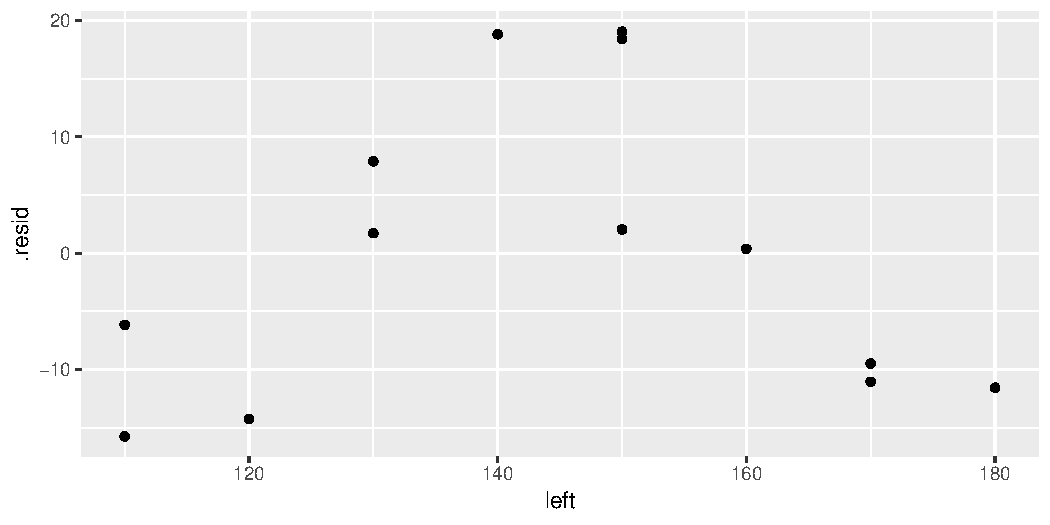
\includegraphics{figure/basingstoke-1.pdf}
\caption{plot of chunk basingstoke}
\end{figure}

\end{frame}

\begin{frame}[fragile]{Comments}
\protect\hypertarget{comments-8}{}

\begin{itemize}
\item
  There is a \emph{curved} relationship with \texttt{left}.
\item
  We should add \texttt{left}-squared to the regression (and therefore
  put \texttt{left} back in when we do that):
\end{itemize}

\begin{Shaded}
\begin{Highlighting}[]
\NormalTok{punting}\FloatTok{.3}\NormalTok{ <-}\StringTok{ }\KeywordTok{lm}\NormalTok{(punt }\OperatorTok{~}\StringTok{ }\NormalTok{left }\OperatorTok{+}\StringTok{ }\KeywordTok{I}\NormalTok{(left}\OperatorTok{^}\DecValTok{2}\NormalTok{) }\OperatorTok{+}\StringTok{ }\NormalTok{right,}
  \DataTypeTok{data =}\NormalTok{ punting}
\NormalTok{)}
\end{Highlighting}
\end{Shaded}

\end{frame}

\begin{frame}[fragile]{Regression with \texttt{left-squared}}
\protect\hypertarget{regression-with-left-squared}{}

\scriptsize

\begin{Shaded}
\begin{Highlighting}[]
\KeywordTok{summary}\NormalTok{(punting}\FloatTok{.3}\NormalTok{)}
\end{Highlighting}
\end{Shaded}

\begin{verbatim}
## 
## Call:
## lm(formula = punt ~ left + I(left^2) + right, data = punting)
## 
## Residuals:
##      Min       1Q   Median       3Q      Max 
## -11.3777  -5.3599   0.0459   4.5088  13.2669 
## 
## Coefficients:
##               Estimate Std. Error t value Pr(>|t|)   
## (Intercept) -4.623e+02  9.902e+01  -4.669  0.00117 **
## left         6.888e+00  1.462e+00   4.710  0.00110 **
## I(left^2)   -2.302e-02  4.927e-03  -4.672  0.00117 **
## right        7.396e-01  2.292e-01   3.227  0.01038 * 
## ---
## Signif. codes:  
## 0 '***' 0.001 '**' 0.01 '*' 0.05 '.' 0.1 ' ' 1
## 
## Residual standard error: 7.931 on 9 degrees of freedom
## Multiple R-squared:  0.9352, Adjusted R-squared:  0.9136 
## F-statistic:  43.3 on 3 and 9 DF,  p-value: 1.13e-05
\end{verbatim}

\normalsize

\end{frame}

\begin{frame}[fragile]{Comments}
\protect\hypertarget{comments-9}{}

\begin{itemize}
\item
  This was definitely a good idea (R-squared has clearly increased).
\item
  We would never have seen it without plotting residuals from
  \texttt{punting.2} (without \texttt{left}) against \texttt{left}.
\item
  Negative slope for \texttt{leftsq} means that increased left-leg
  strength only increases punting distance up to a point: beyond that,
  it decreases again.
\end{itemize}

\end{frame}

\hypertarget{logistic-regression-ordinalnominal-response}{%
\section{Logistic regression (ordinal/nominal
response)}\label{logistic-regression-ordinalnominal-response}}

\begin{frame}[fragile]{Logistic regression}
\protect\hypertarget{logistic-regression}{}

\begin{itemize}
\item
  When response variable is measured/counted, regression can work well.
\item
  But what if response is yes/no, lived/died, success/failure?
\item
  Model \emph{probability} of success.
\item
  Probability must be between 0 and 1; need method that ensures this.
\item
  \emph{Logistic regression} does this. In R, is a \emph{generalized
  linear model} with binomial ``family'':
\end{itemize}

\begin{Shaded}
\begin{Highlighting}[]
\KeywordTok{glm}\NormalTok{(y }\OperatorTok{~}\StringTok{ }\NormalTok{x, }\DataTypeTok{family=}\StringTok{"binomial"}\NormalTok{)}
\end{Highlighting}
\end{Shaded}

\begin{itemize}
\tightlist
\item
  Begin with simplest case.
\end{itemize}

\end{frame}

\begin{frame}[fragile]{Packages}
\protect\hypertarget{packages-1}{}

\begin{Shaded}
\begin{Highlighting}[]
\KeywordTok{library}\NormalTok{(MASS)}
\KeywordTok{library}\NormalTok{(tidyverse)}
\KeywordTok{library}\NormalTok{(broom)}
\KeywordTok{library}\NormalTok{(nnet)}
\end{Highlighting}
\end{Shaded}

\end{frame}

\begin{frame}[fragile]{The rats, part 1}
\protect\hypertarget{the-rats-part-1}{}

\begin{itemize}
\tightlist
\item
  Rats given dose of some poison; either live or die:
\end{itemize}

\small

\begin{verbatim}
dose status
0 lived
1 died
2 lived
3 lived
4 died
5 died
\end{verbatim}

\normalsize

\end{frame}

\begin{frame}[fragile]{Read in:}
\protect\hypertarget{read-in}{}

\begin{Shaded}
\begin{Highlighting}[]
\NormalTok{my_url <-}\StringTok{ "http://www.utsc.utoronto.ca/~butler/d29/rat.txt"}
\NormalTok{rats <-}\StringTok{ }\KeywordTok{read_delim}\NormalTok{(my_url, }\StringTok{" "}\NormalTok{)}
\end{Highlighting}
\end{Shaded}

\begin{verbatim}
## Parsed with column specification:
## cols(
##   dose = col_double(),
##   status = col_character()
## )
\end{verbatim}

\begin{Shaded}
\begin{Highlighting}[]
\KeywordTok{glimpse}\NormalTok{(rats)}
\end{Highlighting}
\end{Shaded}

\begin{verbatim}
## Observations: 6
## Variables: 2
## $ dose   <dbl> 0, 1, 2, 3, 4, 5
## $ status <chr> "lived", "died", "lived", "lived", "died",…
\end{verbatim}

\end{frame}

\begin{frame}[fragile]{Basic logistic regression}
\protect\hypertarget{basic-logistic-regression}{}

\begin{itemize}
\tightlist
\item
  Make response into a factor first:
\end{itemize}

\small

\begin{Shaded}
\begin{Highlighting}[]
\NormalTok{rats2 <-}\StringTok{ }\NormalTok{rats }\OperatorTok\StringTok{ }\KeywordTok{mutate}\NormalTok{(}\DataTypeTok{status =} \KeywordTok{factor}\NormalTok{(status))}
\end{Highlighting}
\end{Shaded}

\normalsize

\begin{itemize}
\tightlist
\item
  then fit model:
\end{itemize}

\small

\begin{Shaded}
\begin{Highlighting}[]
\NormalTok{status}\FloatTok{.1}\NormalTok{ <-}\StringTok{ }\KeywordTok{glm}\NormalTok{(status }\OperatorTok{~}\StringTok{ }\NormalTok{dose, }\DataTypeTok{family =} \StringTok{"binomial"}\NormalTok{, }\DataTypeTok{data =}\NormalTok{ rats2)}
\end{Highlighting}
\end{Shaded}

\normalsize

\end{frame}

\begin{frame}[fragile]{Output}
\protect\hypertarget{output-1}{}

\scriptsize

\begin{Shaded}
\begin{Highlighting}[]
\KeywordTok{summary}\NormalTok{(status}\FloatTok{.1}\NormalTok{)}
\end{Highlighting}
\end{Shaded}

\begin{verbatim}
## 
## Call:
## glm(formula = status ~ dose, family = "binomial", data = rats2)
## 
## Deviance Residuals: 
##       1        2        3        4        5        6  
##  0.5835  -1.6254   1.0381   1.3234  -0.7880  -0.5835  
## 
## Coefficients:
##             Estimate Std. Error z value Pr(>|z|)
## (Intercept)   1.6841     1.7979   0.937    0.349
## dose         -0.6736     0.6140  -1.097    0.273
## 
## (Dispersion parameter for binomial family taken to be 1)
## 
##     Null deviance: 8.3178  on 5  degrees of freedom
## Residual deviance: 6.7728  on 4  degrees of freedom
## AIC: 10.773
## 
## Number of Fisher Scoring iterations: 4
\end{verbatim}

\normalsize

\end{frame}

\begin{frame}{Interpreting the output}
\protect\hypertarget{interpreting-the-output}{}

\begin{itemize}
\item
  Like (multiple) regression, get tests of significance of individual
  \(x\)'s
\item
  Here not significant (only 6 observations).
\item
  ``Slope'' for dose is negative, meaning that as dose increases,
  probability of event modelled (survival) decreases.
\end{itemize}

\end{frame}

\begin{frame}[fragile]{Output part 2: predicted survival probs}
\protect\hypertarget{output-part-2-predicted-survival-probs}{}

\begin{Shaded}
\begin{Highlighting}[]
\NormalTok{p <-}\StringTok{ }\KeywordTok{predict}\NormalTok{(status}\FloatTok{.1}\NormalTok{, }\DataTypeTok{type =} \StringTok{"response"}\NormalTok{)}
\KeywordTok{cbind}\NormalTok{(rats, p)}
\end{Highlighting}
\end{Shaded}

\begin{verbatim}
##   dose status         p
## 1    0  lived 0.8434490
## 2    1   died 0.7331122
## 3    2  lived 0.5834187
## 4    3  lived 0.4165813
## 5    4   died 0.2668878
## 6    5   died 0.1565510
\end{verbatim}

\end{frame}

\begin{frame}[fragile]{The rats, more}
\protect\hypertarget{the-rats-more}{}

\begin{itemize}
\item
  More realistic: more rats at each dose (say 10).
\item
  Listing each rat on one line makes a big data file.
\item
  Use format below: dose, number of survivals, number of deaths.
\end{itemize}

\begin{verbatim}

dose lived died
0    10    0
1     7    3 
2     6    4 
3     4    6 
4     2    8 
5     1    9  
\end{verbatim}

\begin{itemize}
\item
  6 lines of data correspond to 60 actual rats.
\item
  Saved in \texttt{rat2.txt}.
\end{itemize}

\end{frame}

\begin{frame}[fragile]{These data}
\protect\hypertarget{these-data}{}

\footnotesize

\begin{Shaded}
\begin{Highlighting}[]
\NormalTok{my_url <-}\StringTok{ "http://www.utsc.utoronto.ca/~butler/d29/rat2.txt"}
\NormalTok{rat2 <-}\StringTok{ }\KeywordTok{read_delim}\NormalTok{(my_url, }\StringTok{" "}\NormalTok{)}
\end{Highlighting}
\end{Shaded}

\begin{verbatim}
## Parsed with column specification:
## cols(
##   dose = col_double(),
##   lived = col_double(),
##   died = col_double()
## )
\end{verbatim}

\begin{Shaded}
\begin{Highlighting}[]
\NormalTok{rat2}
\end{Highlighting}
\end{Shaded}

\begin{verbatim}
## # A tibble: 6 x 3
##    dose lived  died
##   <dbl> <dbl> <dbl>
## 1     0    10     0
## 2     1     7     3
## 3     2     6     4
## 4     3     4     6
## 5     4     2     8
## 6     5     1     9
\end{verbatim}

\normalsize

\end{frame}

\begin{frame}[fragile]{Create response matrix:}
\protect\hypertarget{create-response-matrix}{}

\begin{itemize}
\tightlist
\item
  Each row contains \emph{multiple} observations.
\item
  Create \emph{two-column} response:

  \begin{itemize}
  \tightlist
  \item
    \#survivals in first column,
  \item
    \#deaths in second.
  \end{itemize}
\end{itemize}

\footnotesize

\begin{Shaded}
\begin{Highlighting}[]
\NormalTok{response <-}\StringTok{ }\KeywordTok{with}\NormalTok{(rat2, }\KeywordTok{cbind}\NormalTok{(lived, died))}
\NormalTok{response}
\end{Highlighting}
\end{Shaded}

\begin{verbatim}
##      lived died
## [1,]    10    0
## [2,]     7    3
## [3,]     6    4
## [4,]     4    6
## [5,]     2    8
## [6,]     1    9
\end{verbatim}

\normalsize

\begin{itemize}
\tightlist
\item
  Response is R \texttt{matrix}:
\end{itemize}

\footnotesize

\begin{Shaded}
\begin{Highlighting}[]
\KeywordTok{class}\NormalTok{(response)}
\end{Highlighting}
\end{Shaded}

\begin{verbatim}
## [1] "matrix"
\end{verbatim}

\normalsize

\end{frame}

\begin{frame}[fragile]{Fit logistic regression}
\protect\hypertarget{fit-logistic-regression}{}

\begin{itemize}
\tightlist
\item
  using response you just made:
\end{itemize}

\begin{Shaded}
\begin{Highlighting}[]
\NormalTok{rat2}\FloatTok{.1}\NormalTok{ <-}\StringTok{ }\KeywordTok{glm}\NormalTok{(response }\OperatorTok{~}\StringTok{ }\NormalTok{dose,}
  \DataTypeTok{family =} \StringTok{"binomial"}\NormalTok{,}
  \DataTypeTok{data =}\NormalTok{ rat2}
\NormalTok{)}
\end{Highlighting}
\end{Shaded}

\end{frame}

\begin{frame}[fragile]{Output}
\protect\hypertarget{output-2}{}

\scriptsize

\begin{Shaded}
\begin{Highlighting}[]
\KeywordTok{summary}\NormalTok{(rat2}\FloatTok{.1}\NormalTok{)}
\end{Highlighting}
\end{Shaded}

\begin{verbatim}
## 
## Call:
## glm(formula = response ~ dose, family = "binomial", data = rat2)
## 
## Deviance Residuals: 
##       1        2        3        4        5        6  
##  1.3421  -0.7916  -0.1034   0.1034   0.0389   0.1529  
## 
## Coefficients:
##             Estimate Std. Error z value Pr(>|z|)    
## (Intercept)   2.3619     0.6719   3.515 0.000439 ***
## dose         -0.9448     0.2351  -4.018 5.87e-05 ***
## ---
## Signif. codes:  
## 0 '***' 0.001 '**' 0.01 '*' 0.05 '.' 0.1 ' ' 1
## 
## (Dispersion parameter for binomial family taken to be 1)
## 
##     Null deviance: 27.530  on 5  degrees of freedom
## Residual deviance:  2.474  on 4  degrees of freedom
## AIC: 18.94
## 
## Number of Fisher Scoring iterations: 4
\end{verbatim}

\normalsize

\end{frame}

\begin{frame}[fragile]{Predicted survival probs}
\protect\hypertarget{predicted-survival-probs}{}

\begin{Shaded}
\begin{Highlighting}[]
\NormalTok{p <-}\StringTok{ }\KeywordTok{predict}\NormalTok{(rat2}\FloatTok{.1}\NormalTok{, }\DataTypeTok{type =} \StringTok{"response"}\NormalTok{)}
\KeywordTok{cbind}\NormalTok{(rat2, p)}
\end{Highlighting}
\end{Shaded}

\begin{verbatim}
##   dose lived died         p
## 1    0    10    0 0.9138762
## 2    1     7    3 0.8048905
## 3    2     6    4 0.6159474
## 4    3     4    6 0.3840526
## 5    4     2    8 0.1951095
## 6    5     1    9 0.0861238
\end{verbatim}

\end{frame}

\begin{frame}{Comments}
\protect\hypertarget{comments-10}{}

\begin{itemize}
\item
  Significant effect of dose.
\item
  Effect of larger dose is to \emph{decrease} survival probability
  (``slope'' negative; also see in decreasing predictions.)
\end{itemize}

\end{frame}

\begin{frame}{Multiple logistic regression}
\protect\hypertarget{multiple-logistic-regression}{}

\begin{itemize}
\item
  With more than one \(x\), works much like multiple regression.
\item
  Example: study of patients with blood poisoning severe enough to
  warrant surgery. Relate survival to other potential risk factors.
\item
  Variables, 1=present, 0=absent:

  \begin{itemize}
  \tightlist
  \item
    survival (death from sepsis=1), response
  \item
    shock
  \item
    malnutrition
  \item
    alcoholism
  \item
    age (as numerical variable)
  \item
    bowel infarction
  \end{itemize}
\item
  See what relates to death.
\end{itemize}

\end{frame}

\begin{frame}[fragile]{Read in data}
\protect\hypertarget{read-in-data}{}

\begin{Shaded}
\begin{Highlighting}[]
\NormalTok{my_url <-}\StringTok{ }
\StringTok{  "http://www.utsc.utoronto.ca/~butler/d29/sepsis.txt"}
\NormalTok{sepsis <-}\StringTok{ }\KeywordTok{read_delim}\NormalTok{(my_url, }\StringTok{" "}\NormalTok{)}
\end{Highlighting}
\end{Shaded}

\begin{verbatim}
## Parsed with column specification:
## cols(
##   death = col_double(),
##   shock = col_double(),
##   malnut = col_double(),
##   alcohol = col_double(),
##   age = col_double(),
##   bowelinf = col_double()
## )
\end{verbatim}

\end{frame}

\begin{frame}[fragile]{The data}
\protect\hypertarget{the-data-2}{}

\begin{Shaded}
\begin{Highlighting}[]
\NormalTok{sepsis}
\end{Highlighting}
\end{Shaded}

\begin{verbatim}
## # A tibble: 106 x 6
##    death shock malnut alcohol   age bowelinf
##    <dbl> <dbl>  <dbl>   <dbl> <dbl>    <dbl>
##  1     0     0      0       0    56        0
##  2     0     0      0       0    80        0
##  3     0     0      0       0    61        0
##  4     0     0      0       0    26        0
##  5     0     0      0       0    53        0
##  6     1     0      1       0    87        0
##  7     0     0      0       0    21        0
##  8     1     0      0       1    69        0
##  9     0     0      0       0    57        0
## 10     0     0      1       0    76        0
## # … with 96 more rows
\end{verbatim}

\end{frame}

\begin{frame}[fragile]{Fit model}
\protect\hypertarget{fit-model}{}

\begin{Shaded}
\begin{Highlighting}[]
\NormalTok{sepsis}\FloatTok{.1}\NormalTok{ <-}\StringTok{ }\KeywordTok{glm}\NormalTok{(death }\OperatorTok{~}\StringTok{ }\NormalTok{shock }\OperatorTok{+}\StringTok{ }\NormalTok{malnut }\OperatorTok{+}\StringTok{ }\NormalTok{alcohol }\OperatorTok{+}\StringTok{ }\NormalTok{age }\OperatorTok{+}
\StringTok{  }\NormalTok{bowelinf,}
\DataTypeTok{family =} \StringTok{"binomial"}\NormalTok{,}
\DataTypeTok{data =}\NormalTok{ sepsis}
\NormalTok{)}
\end{Highlighting}
\end{Shaded}

\end{frame}

\begin{frame}[fragile]{Output part 1}
\protect\hypertarget{output-part-1}{}

\begin{Shaded}
\begin{Highlighting}[]
\KeywordTok{tidy}\NormalTok{(sepsis}\FloatTok{.1}\NormalTok{)}
\end{Highlighting}
\end{Shaded}

\begin{verbatim}
## # A tibble: 6 x 5
##   term        estimate std.error statistic  p.value
##   <chr>          <dbl>     <dbl>     <dbl>    <dbl>
## 1 (Intercept)  -9.75      2.54       -3.84 0.000124
## 2 shock         3.67      1.16        3.15 0.00161 
## 3 malnut        1.22      0.728       1.67 0.0948  
## 4 alcohol       3.35      0.982       3.42 0.000635
## 5 age           0.0922    0.0303      3.04 0.00237 
## 6 bowelinf      2.80      1.16        2.40 0.0162
\end{verbatim}

\begin{itemize}
\item
  All P-values fairly small
\item
  but \texttt{malnut} not significant: remove.
\end{itemize}

\end{frame}

\begin{frame}[fragile]{Removing \texttt{malnut}}
\protect\hypertarget{removing-malnut}{}

\begin{Shaded}
\begin{Highlighting}[]
\NormalTok{sepsis}\FloatTok{.2}\NormalTok{ <-}\StringTok{ }\KeywordTok{update}\NormalTok{(sepsis}\FloatTok{.1}\NormalTok{, . }\OperatorTok{~}\StringTok{ }\NormalTok{. }\OperatorTok{-}\StringTok{ }\NormalTok{malnut)}
\KeywordTok{tidy}\NormalTok{(sepsis}\FloatTok{.2}\NormalTok{)}
\end{Highlighting}
\end{Shaded}

\begin{verbatim}
## # A tibble: 5 x 5
##   term        estimate std.error statistic  p.value
##   <chr>          <dbl>     <dbl>     <dbl>    <dbl>
## 1 (Intercept)  -8.89      2.32       -3.84 0.000124
## 2 shock         3.70      1.10        3.35 0.000797
## 3 alcohol       3.19      0.917       3.47 0.000514
## 4 age           0.0898    0.0292      3.07 0.00211 
## 5 bowelinf      2.39      1.07        2.23 0.0260
\end{verbatim}

\begin{itemize}
\tightlist
\item
  Everything significant now.
\end{itemize}

\end{frame}

\begin{frame}[fragile]{Comments}
\protect\hypertarget{comments-11}{}

\begin{itemize}
\item
  Most of the original \(x\)'s helped predict death. Only
  \texttt{malnut} seemed not to add anything.
\item
  Removed \texttt{malnut} and tried again.
\item
  Everything remaining is significant (though \texttt{bowelinf} actually
  became \emph{less} significant).
\item
  All coefficients are \emph{positive}, so having any of the risk
  factors (or being older) \emph{increases} risk of death.
\end{itemize}

\end{frame}

\begin{frame}[fragile]{Predictions from model without ``malnut''}
\protect\hypertarget{predictions-from-model-without-malnut}{}

\begin{itemize}
\tightlist
\item
  A few chosen at random:
\end{itemize}

\normalsize

\begin{Shaded}
\begin{Highlighting}[]
\NormalTok{sepsis.pred <-}\StringTok{ }\KeywordTok{predict}\NormalTok{(sepsis}\FloatTok{.2}\NormalTok{, }\DataTypeTok{type =} \StringTok{"response"}\NormalTok{)}
\NormalTok{d <-}\StringTok{ }\KeywordTok{data.frame}\NormalTok{(sepsis, sepsis.pred)}
\NormalTok{myrows <-}\StringTok{ }\KeywordTok{c}\NormalTok{(}\DecValTok{4}\NormalTok{, }\DecValTok{1}\NormalTok{, }\DecValTok{2}\NormalTok{, }\DecValTok{11}\NormalTok{, }\DecValTok{32}\NormalTok{)}
\KeywordTok{slice}\NormalTok{(d, myrows)}
\end{Highlighting}
\end{Shaded}

\begin{verbatim}
##   death shock malnut alcohol age bowelinf sepsis.pred
## 1     0     0      0       0  26        0 0.001415347
## 2     0     0      0       0  56        0 0.020552383
## 3     0     0      0       0  80        0 0.153416834
## 4     1     0      0       1  66        1 0.931290137
## 5     1     0      0       1  49        0 0.213000997
\end{verbatim}

\normalsize

\end{frame}

\begin{frame}{Comments}
\protect\hypertarget{comments-12}{}

\begin{itemize}
\item
  Survival chances pretty good if no risk factors, though decreasing
  with age.
\item
  Having more than one risk factor reduces survival chances
  dramatically.
\item
  Usually good job of predicting survival; sometimes death predicted to
  survive.
\end{itemize}

\end{frame}

\begin{frame}{Assessing proportionality of odds for age}
\protect\hypertarget{assessing-proportionality-of-odds-for-age}{}

\begin{itemize}
\item
  An assumption we made is that log-odds of survival depends linearly on
  age.
\item
  Hard to get your head around, but basic idea is that survival chances
  go continuously up (or down) with age, instead of (for example) going
  up and then down.
\item
  In this case, seems reasonable, but should check:
\end{itemize}

\end{frame}

\begin{frame}[fragile]{Residuals vs.~age}
\protect\hypertarget{residuals-vs.age}{}

\begin{Shaded}
\begin{Highlighting}[]
\KeywordTok{ggplot}\NormalTok{(}\KeywordTok{augment}\NormalTok{(sepsis}\FloatTok{.2}\NormalTok{), }\KeywordTok{aes}\NormalTok{(}\DataTypeTok{x =}\NormalTok{ age, }\DataTypeTok{y =}\NormalTok{ .resid)) }\OperatorTok{+}
\StringTok{  }\KeywordTok{geom_point}\NormalTok{()}
\end{Highlighting}
\end{Shaded}

\begin{figure}
\centering
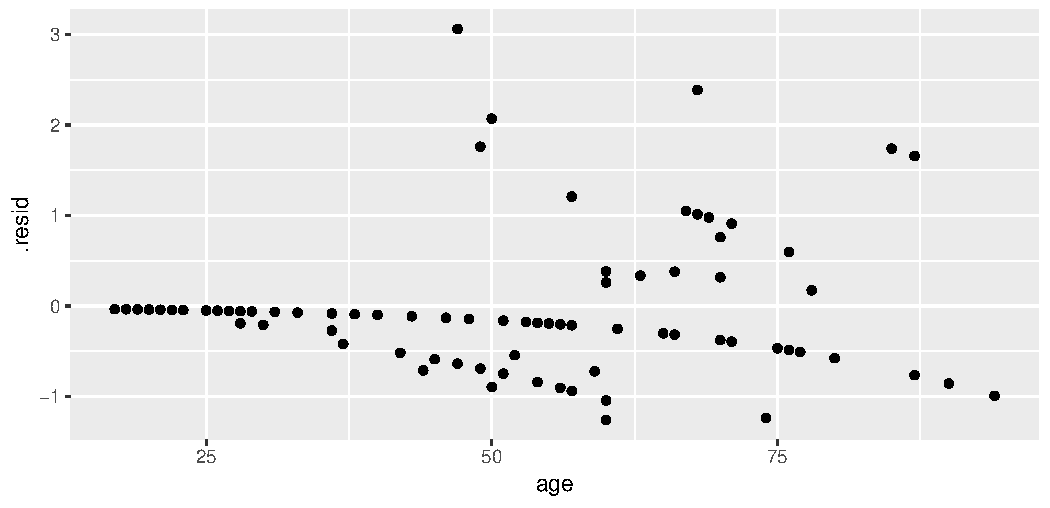
\includegraphics{figure/virtusentella-1.pdf}
\caption{plot of chunk virtusentella}
\end{figure}

\end{frame}

\begin{frame}{Comments}
\protect\hypertarget{comments-13}{}

\begin{itemize}
\item
  No apparent problems overall.
\item
  Confusing ``line'' across: no risk factors, survived.
\end{itemize}

\end{frame}

\begin{frame}{Probability and odds}
\protect\hypertarget{probability-and-odds}{}

\begin{itemize}
\item
  For probability \(p\), odds is \(p/(1-p)\):

  \begin{tabular}{rrrl}
      \hline
      Prob.\ & Odds & log-odds & in words\\
      \hline
      0.5 & $0.5/0.5=1/1=1.00$ & $0.00$ &  ``even money''\\
      0.1 & $0.1/0.9=1/9=0.11$ & $-2.20$ & ``9 to 1''\\
      0.4 & $0.4/0.6=1/1.5=0.67$ & $-0.41$ & ``1.5 to 1''\\
      0.8 & $0.8/0.2=4/1=4.00$ & $1.39$ & ``4 to 1 on''\\
      \hline
    \end{tabular}
\item
  Gamblers use odds: if you win at 9 to 1 odds, get original stake back
  plus 9 times the stake.
\item
  Probability has to be between 0 and 1
\item
  Odds between 0 and infinity
\item
  \emph{Log}-odds can be anything: any log-odds corresponds to valid
  probability.
\end{itemize}

\end{frame}

\begin{frame}{Odds ratio}
\protect\hypertarget{odds-ratio}{}

\begin{itemize}
\item
  Suppose 90 of 100 men drank wine last week, but only 20 of 100 women.
\item
  Prob of man drinking wine \(90/100=0.9\), woman \(20/100=0.2\).
\item
  Odds of man drinking wine \(0.9/0.1=9\), woman \(0.2/0.8=0.25\).
\item
  Ratio of odds is \(9/0.25=36\).
\item
  Way of quantifying difference between men and women: ``odds of
  drinking wine 36 times larger for males than females''.
\end{itemize}

\end{frame}

\begin{frame}[fragile]{Sepsis data again}
\protect\hypertarget{sepsis-data-again}{}

\begin{itemize}
\tightlist
\item
  Recall prediction of probability of death from risk factors:
\end{itemize}

\begin{Shaded}
\begin{Highlighting}[]
\NormalTok{sepsis.}\FloatTok{2.}\NormalTok{tidy <-}\StringTok{ }\KeywordTok{tidy}\NormalTok{(sepsis}\FloatTok{.2}\NormalTok{)}
\NormalTok{sepsis.}\FloatTok{2.}\NormalTok{tidy}
\end{Highlighting}
\end{Shaded}

\begin{verbatim}
## # A tibble: 5 x 5
##   term        estimate std.error statistic  p.value
##   <chr>          <dbl>     <dbl>     <dbl>    <dbl>
## 1 (Intercept)  -8.89      2.32       -3.84 0.000124
## 2 shock         3.70      1.10        3.35 0.000797
## 3 alcohol       3.19      0.917       3.47 0.000514
## 4 age           0.0898    0.0292      3.07 0.00211 
## 5 bowelinf      2.39      1.07        2.23 0.0260
\end{verbatim}

\begin{itemize}
\tightlist
\item
  Slopes in column \texttt{estimate}.
\end{itemize}

\end{frame}

\begin{frame}[fragile]{Multiplying the odds}
\protect\hypertarget{multiplying-the-odds}{}

\begin{itemize}
\tightlist
\item
  Can interpret slopes by taking ``exp'' of them. We ignore intercept.
\end{itemize}

\begin{Shaded}
\begin{Highlighting}[]
\NormalTok{sepsis.}\FloatTok{2.}\NormalTok{tidy }\OperatorTok\StringTok{ }
\StringTok{  }\KeywordTok{mutate}\NormalTok{(}\DataTypeTok{exp_coeff=}\KeywordTok{exp}\NormalTok{(estimate)) }\OperatorTok\StringTok{ }
\StringTok{  }\KeywordTok{select}\NormalTok{(term, exp_coeff)}
\end{Highlighting}
\end{Shaded}

\begin{verbatim}
## # A tibble: 5 x 2
##   term        exp_coeff
##   <chr>           <dbl>
## 1 (Intercept)  0.000137
## 2 shock       40.5     
## 3 alcohol     24.2     
## 4 age          1.09    
## 5 bowelinf    10.9
\end{verbatim}

\end{frame}

\begin{frame}[fragile]{Interpretation}
\protect\hypertarget{interpretation}{}

\small

\begin{verbatim}
## # A tibble: 5 x 2
##   term        exp_coeff
##   <chr>           <dbl>
## 1 (Intercept)  0.000137
## 2 shock       40.5     
## 3 alcohol     24.2     
## 4 age          1.09    
## 5 bowelinf    10.9
\end{verbatim}

\normalsize

\begin{itemize}
\item
  These say ``how much do you \emph{multiply} odds of death by for
  increase of 1 in corresponding risk factor?'' Or, what is odds ratio
  for that factor being 1 (present) vs.~0 (absent)?
\item
  Eg.~being alcoholic vs.~not increases odds of death by 24 times
\item
  One year older multiplies odds by about 1.1 times. Over 40 years,
  about \(1.09^{40}=31\) times.
\end{itemize}

\end{frame}

\begin{frame}{Odds ratio and relative risk}
\protect\hypertarget{odds-ratio-and-relative-risk}{}

\begin{itemize}
\item
  \textbf{Relative risk} is ratio of probabilities.
\item
  Above: 90 of 100 men (0.9) drank wine, 20 of 100 women (0.2).
\item
  Relative risk 0.9/0.2=4.5. (odds ratio was 36).
\item
  When probabilities small, relative risk and odds ratio similar.
\item
  Eg.~prob of man having disease 0.02, woman 0.01.
\item
  Relative risk \(0.02/0.01=2\).
\end{itemize}

\end{frame}

\begin{frame}[fragile]{Odds ratio vs.~relative risk}
\protect\hypertarget{odds-ratio-vs.relative-risk}{}

\begin{itemize}
\tightlist
\item
  Odds for men and for women:
\end{itemize}

\begin{Shaded}
\begin{Highlighting}[]
\NormalTok{(od1 <-}\StringTok{ }\FloatTok{0.02} \OperatorTok{/}\StringTok{ }\FloatTok{0.98}\NormalTok{) }\CommentTok{# men}
\end{Highlighting}
\end{Shaded}

\begin{verbatim}
## [1] 0.02040816
\end{verbatim}

\begin{Shaded}
\begin{Highlighting}[]
\NormalTok{(od2 <-}\StringTok{ }\FloatTok{0.01} \OperatorTok{/}\StringTok{ }\FloatTok{0.99}\NormalTok{) }\CommentTok{# women}
\end{Highlighting}
\end{Shaded}

\begin{verbatim}
## [1] 0.01010101
\end{verbatim}

\begin{itemize}
\tightlist
\item
  Odds ratio
\end{itemize}

\begin{Shaded}
\begin{Highlighting}[]
\NormalTok{od1 }\OperatorTok{/}\StringTok{ }\NormalTok{od2}
\end{Highlighting}
\end{Shaded}

\begin{verbatim}
## [1] 2.020408
\end{verbatim}

\begin{itemize}
\tightlist
\item
  Very close to relative risk of 2.
\end{itemize}

\end{frame}

\begin{frame}{More than 2 response categories}
\protect\hypertarget{more-than-2-response-categories}{}

\begin{itemize}
\item
  With 2 response categories, model the probability of one, and prob of
  other is one minus that. So doesn't matter which category you model.
\item
  With more than 2 categories, have to think more carefully about the
  categories: are they
\item
  \emph{ordered}: you can put them in a natural order (like low, medium,
  high)
\item
  \emph{nominal}: ordering the categories doesn't make sense (like red,
  green, blue).
\item
  R handles both kinds of response; learn how.
\end{itemize}

\end{frame}

\begin{frame}{Ordinal response: the miners}
\protect\hypertarget{ordinal-response-the-miners}{}

\begin{itemize}
\item
  Model probability of being in given category \emph{or lower}.
\item
  Example: coal-miners often suffer disease pneumoconiosis. Likelihood
  of disease believed to be greater among miners who have worked longer.
\item
  Severity of disease measured on categorical scale: none, moderate, 3
  severe.
\end{itemize}

\end{frame}

\begin{frame}[fragile]{Miners data}
\protect\hypertarget{miners-data}{}

\begin{itemize}
\tightlist
\item
  Data are frequencies:
\end{itemize}

\begin{verbatim}
Exposure None Moderate Severe
5.8       98      0       0
15.0      51      2       1
21.5      34      6       3
27.5      35      5       8
33.5      32     10       9
39.5      23      7       8
46.0      12      6      10
51.5       4      2       5
\end{verbatim}

\end{frame}

\begin{frame}[fragile]{Reading the data}
\protect\hypertarget{reading-the-data}{}

Data in aligned columns with more than one space between, so:

\small

\begin{Shaded}
\begin{Highlighting}[]
\NormalTok{my_url <-}\StringTok{ "http://www.utsc.utoronto.ca/~butler/d29/miners-tab.txt"}
\NormalTok{freqs <-}\StringTok{ }\KeywordTok{read_table}\NormalTok{(my_url)}
\end{Highlighting}
\end{Shaded}

\begin{verbatim}
## Parsed with column specification:
## cols(
##   Exposure = col_double(),
##   None = col_double(),
##   Moderate = col_double(),
##   Severe = col_double()
## )
\end{verbatim}

\normalsize

\end{frame}

\begin{frame}[fragile]{The data}
\protect\hypertarget{the-data-3}{}

\begin{Shaded}
\begin{Highlighting}[]
\NormalTok{freqs}
\end{Highlighting}
\end{Shaded}

\begin{verbatim}
## # A tibble: 8 x 4
##   Exposure  None Moderate Severe
##      <dbl> <dbl>    <dbl>  <dbl>
## 1      5.8    98        0      0
## 2     15      51        2      1
## 3     21.5    34        6      3
## 4     27.5    35        5      8
## 5     33.5    32       10      9
## 6     39.5    23        7      8
## 7     46      12        6     10
## 8     51.5     4        2      5
\end{verbatim}

\end{frame}

\begin{frame}[fragile]{Tidying and row proportions}
\protect\hypertarget{tidying-and-row-proportions}{}

\begin{Shaded}
\begin{Highlighting}[]
\NormalTok{freqs }\OperatorTok
\StringTok{  }\KeywordTok{gather}\NormalTok{(Severity, Freq, None}\OperatorTok{:}\NormalTok{Severe) }\OperatorTok
\StringTok{  }\KeywordTok{group_by}\NormalTok{(Exposure) }\OperatorTok
\StringTok{  }\KeywordTok{mutate}\NormalTok{(}\DataTypeTok{proportion =}\NormalTok{ Freq }\OperatorTok{/}\StringTok{ }\KeywordTok{sum}\NormalTok{(Freq)) ->}\StringTok{ }\NormalTok{miners}
\end{Highlighting}
\end{Shaded}

\end{frame}

\begin{frame}[fragile]{Result}
\protect\hypertarget{result}{}

\small

\begin{Shaded}
\begin{Highlighting}[]
\NormalTok{miners}
\end{Highlighting}
\end{Shaded}

\begin{verbatim}
## # A tibble: 24 x 4
## # Groups:   Exposure [8]
##    Exposure Severity  Freq proportion
##       <dbl> <chr>    <dbl>      <dbl>
##  1      5.8 None        98     1     
##  2     15   None        51     0.944 
##  3     21.5 None        34     0.791 
##  4     27.5 None        35     0.729 
##  5     33.5 None        32     0.627 
##  6     39.5 None        23     0.605 
##  7     46   None        12     0.429 
##  8     51.5 None         4     0.364 
##  9      5.8 Moderate     0     0     
## 10     15   Moderate     2     0.0370
## # … with 14 more rows
\end{verbatim}

\normalsize

\end{frame}

\begin{frame}[fragile]{Plot proportions against exposure}
\protect\hypertarget{plot-proportions-against-exposure}{}

\small

\begin{Shaded}
\begin{Highlighting}[]
\KeywordTok{ggplot}\NormalTok{(miners, }\KeywordTok{aes}\NormalTok{(}\DataTypeTok{x =}\NormalTok{ Exposure, }\DataTypeTok{y =}\NormalTok{ proportion,}
                   \DataTypeTok{colour =}\NormalTok{ Severity)) }\OperatorTok{+}\StringTok{ }
\StringTok{  }\KeywordTok{geom_point}\NormalTok{() }\OperatorTok{+}\StringTok{ }\KeywordTok{geom_smooth}\NormalTok{(}\DataTypeTok{se =}\NormalTok{ F)}
\end{Highlighting}
\end{Shaded}

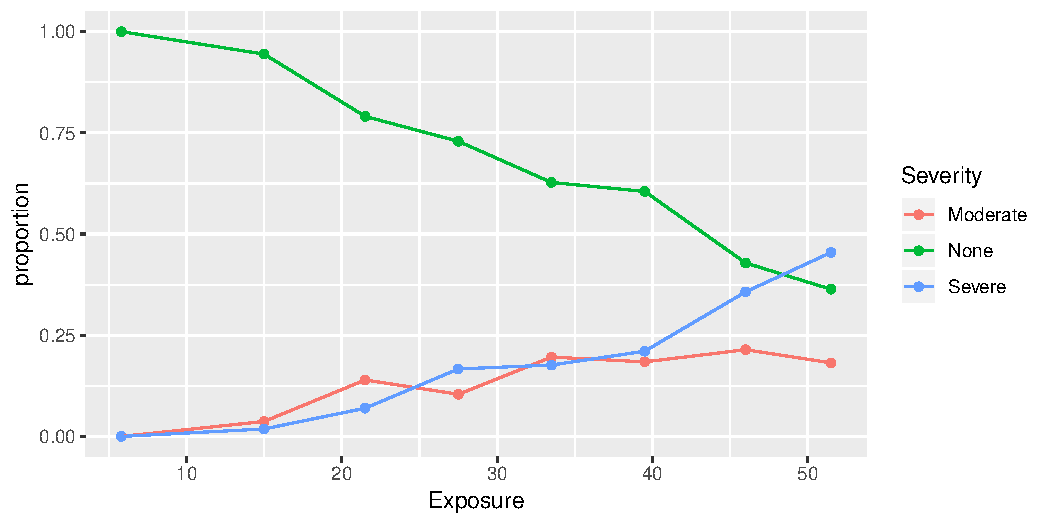
\includegraphics{figure/unnamed-chunk-85-1.pdf} \normalsize

\end{frame}

\begin{frame}[fragile]{Reminder of data setup}
\protect\hypertarget{reminder-of-data-setup}{}

\footnotesize

\begin{Shaded}
\begin{Highlighting}[]
\NormalTok{miners}
\end{Highlighting}
\end{Shaded}

\begin{verbatim}
## # A tibble: 24 x 4
## # Groups:   Exposure [8]
##    Exposure Severity  Freq proportion
##       <dbl> <chr>    <dbl>      <dbl>
##  1      5.8 None        98     1     
##  2     15   None        51     0.944 
##  3     21.5 None        34     0.791 
##  4     27.5 None        35     0.729 
##  5     33.5 None        32     0.627 
##  6     39.5 None        23     0.605 
##  7     46   None        12     0.429 
##  8     51.5 None         4     0.364 
##  9      5.8 Moderate     0     0     
## 10     15   Moderate     2     0.0370
## # … with 14 more rows
\end{verbatim}

\normalsize

\end{frame}

\begin{frame}[fragile]{Creating an ordered factor}
\protect\hypertarget{creating-an-ordered-factor}{}

\begin{itemize}
\item
  Problem: on plot, \texttt{Severity} categories in \emph{wrong
  order}.
\item
  \emph{In the data frame}, categories in \emph{correct} order.
\item
  Package \texttt{forcats} (in \texttt{tidyverse}) has functions for
  creating factors to specifications.
\item
  \texttt{fct\_inorder} takes levels \emph{in order they appear in
  data}:
\end{itemize}

\begin{Shaded}
\begin{Highlighting}[]
\NormalTok{miners }\OperatorTok
\StringTok{  }\KeywordTok{mutate}\NormalTok{(}\DataTypeTok{sev_ord =} \KeywordTok{fct_inorder}\NormalTok{(Severity)) ->}\StringTok{ }\NormalTok{miners}
\end{Highlighting}
\end{Shaded}

\begin{itemize}
\tightlist
\item
  To check:
\end{itemize}

\begin{Shaded}
\begin{Highlighting}[]
\KeywordTok{levels}\NormalTok{(miners}\OperatorTok{$}\NormalTok{sev_ord)}
\end{Highlighting}
\end{Shaded}

\begin{verbatim}
## [1] "None"     "Moderate" "Severe"
\end{verbatim}

\end{frame}

\begin{frame}[fragile]{New data frame}
\protect\hypertarget{new-data-frame}{}

\small

\begin{Shaded}
\begin{Highlighting}[]
\NormalTok{miners}
\end{Highlighting}
\end{Shaded}

\begin{verbatim}
## # A tibble: 24 x 5
## # Groups:   Exposure [8]
##    Exposure Severity  Freq proportion sev_ord 
##       <dbl> <chr>    <dbl>      <dbl> <fct>   
##  1      5.8 None        98     1      None    
##  2     15   None        51     0.944  None    
##  3     21.5 None        34     0.791  None    
##  4     27.5 None        35     0.729  None    
##  5     33.5 None        32     0.627  None    
##  6     39.5 None        23     0.605  None    
##  7     46   None        12     0.429  None    
##  8     51.5 None         4     0.364  None    
##  9      5.8 Moderate     0     0      Moderate
## 10     15   Moderate     2     0.0370 Moderate
## # … with 14 more rows
\end{verbatim}

\normalsize

\end{frame}

\begin{frame}[fragile]{Improved plot}
\protect\hypertarget{improved-plot}{}

\begin{Shaded}
\begin{Highlighting}[]
\KeywordTok{ggplot}\NormalTok{(miners, }\KeywordTok{aes}\NormalTok{(}\DataTypeTok{x =}\NormalTok{ Exposure, }\DataTypeTok{y =}\NormalTok{ proportion,}
                   \DataTypeTok{colour =}\NormalTok{ sev_ord)) }\OperatorTok{+}\StringTok{ }
\StringTok{  }\KeywordTok{geom_point}\NormalTok{() }\OperatorTok{+}\StringTok{ }\KeywordTok{geom_smooth}\NormalTok{(}\DataTypeTok{se =}\NormalTok{ F)}
\end{Highlighting}
\end{Shaded}

\begin{figure}
\centering
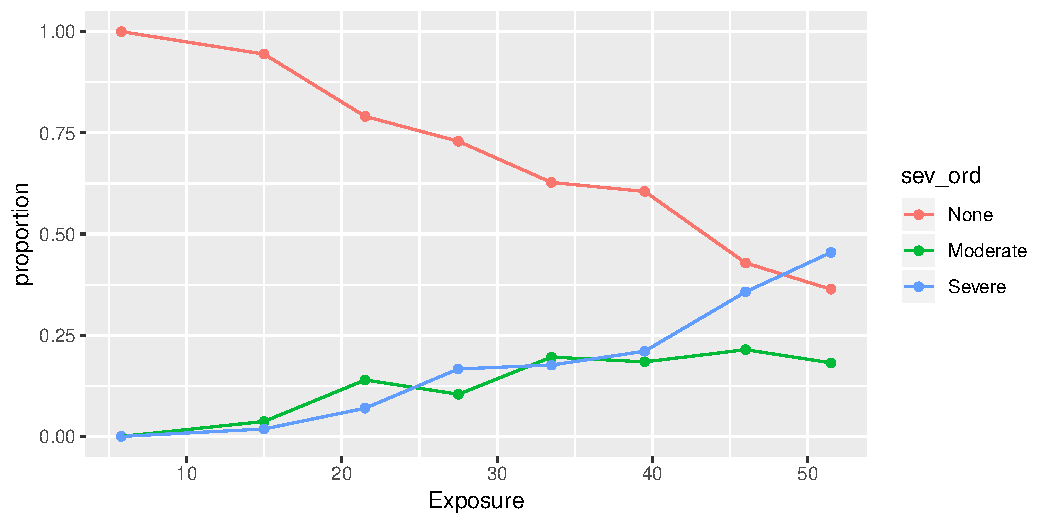
\includegraphics{figure/unnamed-chunk-90-1.pdf}
\caption{plot of chunk unnamed-chunk-90}
\end{figure}

\end{frame}

\begin{frame}[fragile]{Fitting ordered logistic model}
\protect\hypertarget{fitting-ordered-logistic-model}{}

Use function \texttt{polr} from package \texttt{MASS}. Like
\texttt{glm}.

\begin{Shaded}
\begin{Highlighting}[]
\NormalTok{sev}\FloatTok{.1}\NormalTok{ <-}\StringTok{ }\KeywordTok{polr}\NormalTok{(sev_ord }\OperatorTok{~}\StringTok{ }\NormalTok{Exposure,}
  \DataTypeTok{weights =}\NormalTok{ Freq,}
  \DataTypeTok{data =}\NormalTok{ miners}
\NormalTok{)}
\end{Highlighting}
\end{Shaded}

\end{frame}

\begin{frame}[fragile]{Output: not very illuminating}
\protect\hypertarget{output-not-very-illuminating}{}

\scriptsize

\begin{Shaded}
\begin{Highlighting}[]
\KeywordTok{summary}\NormalTok{(sev}\FloatTok{.1}\NormalTok{)}
\end{Highlighting}
\end{Shaded}

\begin{verbatim}
## 
## Re-fitting to get Hessian
\end{verbatim}

\begin{verbatim}
## Call:
## polr(formula = sev_ord ~ Exposure, data = miners, weights = Freq)
## 
## Coefficients:
##           Value Std. Error t value
## Exposure 0.0959    0.01194   8.034
## 
## Intercepts:
##                 Value   Std. Error t value
## None|Moderate    3.9558  0.4097     9.6558
## Moderate|Severe  4.8690  0.4411    11.0383
## 
## Residual Deviance: 416.9188 
## AIC: 422.9188
\end{verbatim}

\normalsize

\end{frame}

\begin{frame}[fragile]{Does exposure have an effect?}
\protect\hypertarget{does-exposure-have-an-effect}{}

Fit model without \texttt{Exposure}, and compare using \texttt{anova}.
Note \texttt{1} for model with just intercept:

\small

\begin{Shaded}
\begin{Highlighting}[]
\NormalTok{sev}\FloatTok{.0}\NormalTok{ <-}\StringTok{ }\KeywordTok{polr}\NormalTok{(sev_ord }\OperatorTok{~}\StringTok{ }\DecValTok{1}\NormalTok{, }\DataTypeTok{weights =}\NormalTok{ Freq, }\DataTypeTok{data =}\NormalTok{ miners)}
\KeywordTok{anova}\NormalTok{(sev}\FloatTok{.0}\NormalTok{, sev}\FloatTok{.1}\NormalTok{)}
\end{Highlighting}
\end{Shaded}

\begin{verbatim}
## Likelihood ratio tests of ordinal regression models
## 
## Response: sev_ord
##      Model Resid. df Resid. Dev   Test
## 1        1       369   505.1621       
## 2 Exposure       368   416.9188 1 vs 2
##      Df LR stat. Pr(Chi)
## 1                       
## 2     1 88.24324       0
\end{verbatim}

\normalsize

Exposure definitely has effect on severity of disease.

\end{frame}

\begin{frame}[fragile]{Another way}
\protect\hypertarget{another-way}{}

\begin{itemize}
\tightlist
\item
  What (if anything) can we drop from model with \texttt{exposure}?
\end{itemize}

\begin{Shaded}
\begin{Highlighting}[]
\KeywordTok{drop1}\NormalTok{(sev}\FloatTok{.1}\NormalTok{, }\DataTypeTok{test =} \StringTok{"Chisq"}\NormalTok{)}
\end{Highlighting}
\end{Shaded}

\begin{verbatim}
## Single term deletions
## 
## Model:
## sev_ord ~ Exposure
##          Df    AIC    LRT  Pr(>Chi)    
## <none>      422.92                     
## Exposure  1 509.16 88.243 < 2.2e-16 ***
## ---
## Signif. codes:  
##   0 '***' 0.001 '**' 0.01 '*' 0.05
##   '.' 0.1 ' ' 1
\end{verbatim}

\begin{itemize}
\tightlist
\item
  Nothing. Exposure definitely has effect.
\end{itemize}

\end{frame}

\begin{frame}[fragile]{Predicted probabilities}
\protect\hypertarget{predicted-probabilities}{}

Make new data frame out of all the exposure values (from original data
frame), and predict from that:

\begin{Shaded}
\begin{Highlighting}[]
\NormalTok{sev.new <-}\StringTok{ }\KeywordTok{tibble}\NormalTok{(}\DataTypeTok{Exposure =}\NormalTok{ freqs}\OperatorTok{$}\NormalTok{Exposure)}
\NormalTok{pr <-}\StringTok{ }\KeywordTok{predict}\NormalTok{(sev}\FloatTok{.1}\NormalTok{, sev.new, }\DataTypeTok{type =} \StringTok{"p"}\NormalTok{)}
\NormalTok{miners.pred <-}\StringTok{ }\KeywordTok{cbind}\NormalTok{(sev.new, pr)}
\NormalTok{miners.pred}
\end{Highlighting}
\end{Shaded}

\begin{verbatim}
##   Exposure      None   Moderate     Severe
## 1      5.8 0.9676920 0.01908912 0.01321885
## 2     15.0 0.9253445 0.04329931 0.03135614
## 3     21.5 0.8692003 0.07385858 0.05694115
## 4     27.5 0.7889290 0.11413004 0.09694093
## 5     33.5 0.6776641 0.16207145 0.16026444
## 6     39.5 0.5418105 0.20484198 0.25334756
## 7     46.0 0.3879962 0.22441555 0.38758828
## 8     51.5 0.2722543 0.21025011 0.51749563
\end{verbatim}

\end{frame}

\begin{frame}[fragile]{Comments}
\protect\hypertarget{comments-14}{}

\begin{itemize}
\item
  Model appears to match data: as exposure goes up, prob of None goes
  down, Severe goes up (sharply for high exposure).
\item
  Like original data frame, this one nice to look at but \emph{not
  tidy}. We want to make graph, so tidy it.
\item
  Also want the severity values in right order.
\item
  Usual \texttt{gather}, plus a bit:
\end{itemize}

\begin{Shaded}
\begin{Highlighting}[]
\NormalTok{miners.pred }\OperatorTok
\StringTok{  }\KeywordTok{gather}\NormalTok{(Severity, probability, }\OperatorTok{-}\NormalTok{Exposure) }\OperatorTok
\StringTok{  }\KeywordTok{mutate}\NormalTok{(}\DataTypeTok{sev_ord =} \KeywordTok{fct_inorder}\NormalTok{(Severity)) ->}\StringTok{ }\NormalTok{preds}
\end{Highlighting}
\end{Shaded}

\end{frame}

\begin{frame}[fragile]{Some of the gathered predictions}
\protect\hypertarget{some-of-the-gathered-predictions}{}

\footnotesize

\begin{Shaded}
\begin{Highlighting}[]
\NormalTok{preds }\OperatorTok\StringTok{ }\KeywordTok{slice}\NormalTok{(}\DecValTok{1}\OperatorTok{:}\DecValTok{15}\NormalTok{)}
\end{Highlighting}
\end{Shaded}

\begin{verbatim}
##    Exposure Severity probability  sev_ord
## 1       5.8     None  0.96769203     None
## 2      15.0     None  0.92534455     None
## 3      21.5     None  0.86920028     None
## 4      27.5     None  0.78892903     None
## 5      33.5     None  0.67766411     None
## 6      39.5     None  0.54181046     None
## 7      46.0     None  0.38799618     None
## 8      51.5     None  0.27225426     None
## 9       5.8 Moderate  0.01908912 Moderate
## 10     15.0 Moderate  0.04329931 Moderate
## 11     21.5 Moderate  0.07385858 Moderate
## 12     27.5 Moderate  0.11413004 Moderate
## 13     33.5 Moderate  0.16207145 Moderate
## 14     39.5 Moderate  0.20484198 Moderate
## 15     46.0 Moderate  0.22441555 Moderate
\end{verbatim}

\normalsize

\end{frame}

\begin{frame}[fragile]{Plotting predicted and observed proportions}
\protect\hypertarget{plotting-predicted-and-observed-proportions}{}

\begin{itemize}
\tightlist
\item
  Plot:

  \begin{itemize}
  \item
    predicted probabilities, lines (shown) joining points (not shown)
  \item
    data, just the points.
  \end{itemize}
\item
  Unfamiliar process: data from two \emph{different} data frames:
\end{itemize}

\small

\begin{Shaded}
\begin{Highlighting}[]
\NormalTok{g <-}\StringTok{ }\KeywordTok{ggplot}\NormalTok{(preds, }\KeywordTok{aes}\NormalTok{(}
  \DataTypeTok{x =}\NormalTok{ Exposure, }\DataTypeTok{y =}\NormalTok{ probability,}
  \DataTypeTok{colour =}\NormalTok{ sev_ord}
\NormalTok{)) }\OperatorTok{+}\StringTok{ }\KeywordTok{geom_line}\NormalTok{() }\OperatorTok{+}
\StringTok{  }\KeywordTok{geom_point}\NormalTok{(}\DataTypeTok{data =}\NormalTok{ miners, }\KeywordTok{aes}\NormalTok{(}\DataTypeTok{y =}\NormalTok{ proportion))}
\end{Highlighting}
\end{Shaded}

\normalsize

\begin{itemize}
\tightlist
\item
  Idea: final \texttt{geom\_point} uses data in \texttt{miners} rather
  than \texttt{preds}, \(y\)-variable for plot is \texttt{proportion}
  from that data frame, but \(x\)-coordinate is \texttt{Exposure}, as it
  was before, and \texttt{colour} is \texttt{Severity} as before. The
  final \texttt{geom\_point} ``inherits'' from the first \texttt{aes} as
  needed.
\end{itemize}

\end{frame}

\begin{frame}[fragile]{The plot: data match model}
\protect\hypertarget{the-plot-data-match-model}{}

\begin{Shaded}
\begin{Highlighting}[]
\NormalTok{g}
\end{Highlighting}
\end{Shaded}

\begin{figure}
\centering
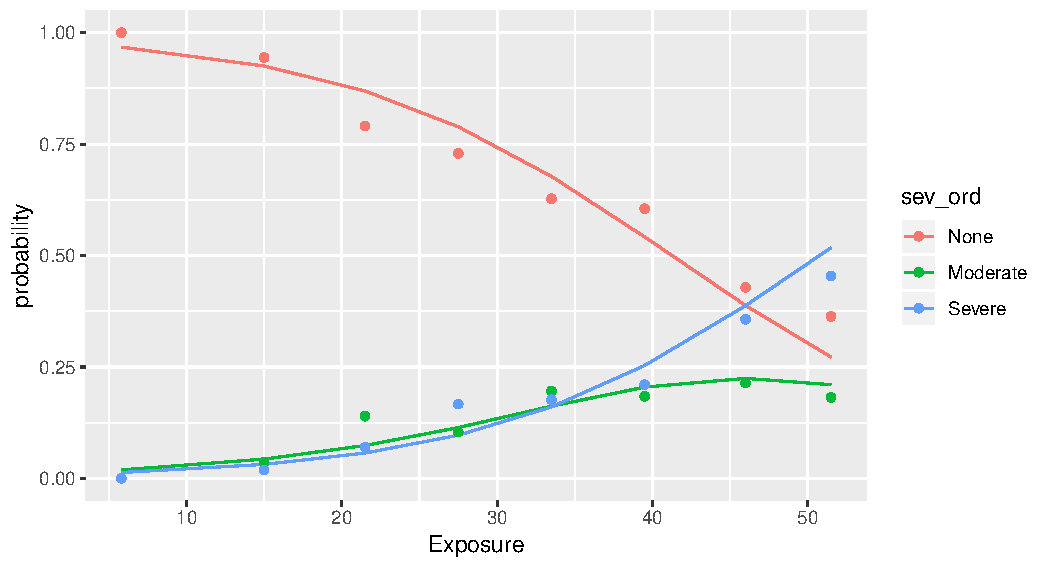
\includegraphics{figure/unnamed-chunk-101-1.pdf}
\caption{plot of chunk unnamed-chunk-101}
\end{figure}

\end{frame}

\begin{frame}[fragile]{Unordered responses}
\protect\hypertarget{unordered-responses}{}

\begin{itemize}
\item
  With unordered (nominal) responses, can use \emph{generalized logit}.
\item
  Example: 735 people, record age and sex (male 0, female 1), which of 3
  brands of some product preferred.
\item
  Data in \texttt{mlogit.csv} separated by commas (so \texttt{read\_csv}
  will work):
\end{itemize}

\begin{Shaded}
\begin{Highlighting}[]
\NormalTok{my_url <-}\StringTok{ "http://www.utsc.utoronto.ca/~butler/d29/mlogit.csv"}
\NormalTok{brandpref <-}\StringTok{ }\KeywordTok{read_csv}\NormalTok{(my_url)}
\end{Highlighting}
\end{Shaded}

\begin{verbatim}
## Parsed with column specification:
## cols(
##   brand = col_double(),
##   sex = col_double(),
##   age = col_double()
## )
\end{verbatim}

\end{frame}

\begin{frame}[fragile]{The data}
\protect\hypertarget{the-data-4}{}

\begin{Shaded}
\begin{Highlighting}[]
\NormalTok{brandpref}
\end{Highlighting}
\end{Shaded}

\begin{verbatim}
## # A tibble: 735 x 3
##    brand   sex   age
##    <dbl> <dbl> <dbl>
##  1     1     0    24
##  2     1     0    26
##  3     1     0    26
##  4     1     1    27
##  5     1     1    27
##  6     3     1    27
##  7     1     0    27
##  8     1     0    27
##  9     1     1    27
## 10     1     0    27
## # … with 725 more rows
\end{verbatim}

\end{frame}

\begin{frame}[fragile]{Bashing into shape, and fitting model}
\protect\hypertarget{bashing-into-shape-and-fitting-model}{}

\begin{itemize}
\tightlist
\item
  \texttt{sex} and \texttt{brand} not meaningful as numbers, so turn
  into factors:
\end{itemize}

\begin{Shaded}
\begin{Highlighting}[]
\NormalTok{brandpref <-}\StringTok{ }\NormalTok{brandpref }\OperatorTok
\StringTok{  }\KeywordTok{mutate}\NormalTok{(}\DataTypeTok{sex =} \KeywordTok{factor}\NormalTok{(sex)) }\OperatorTok
\StringTok{  }\KeywordTok{mutate}\NormalTok{(}\DataTypeTok{brand =} \KeywordTok{factor}\NormalTok{(brand))}
\end{Highlighting}
\end{Shaded}

\begin{itemize}
\tightlist
\item
  We use \texttt{multinom} from package \texttt{nnet}. Works like
  \texttt{polr}.
\end{itemize}

\begin{Shaded}
\begin{Highlighting}[]
\NormalTok{brands}\FloatTok{.1}\NormalTok{ <-}\StringTok{ }\KeywordTok{multinom}\NormalTok{(brand }\OperatorTok{~}\StringTok{ }\NormalTok{age }\OperatorTok{+}\StringTok{ }\NormalTok{sex, }\DataTypeTok{data =}\NormalTok{ brandpref)}
\end{Highlighting}
\end{Shaded}

\begin{verbatim}
## # weights:  12 (6 variable)
## initial  value 807.480032 
## iter  10 value 702.976983
## final  value 702.970704 
## converged
\end{verbatim}

\end{frame}

\begin{frame}[fragile]{Can we drop anything?}
\protect\hypertarget{can-we-drop-anything}{}

\begin{itemize}
\tightlist
\item
  Unfortunately \texttt{drop1} seems not to work:
\end{itemize}

\begin{Shaded}
\begin{Highlighting}[]
\KeywordTok{drop1}\NormalTok{(brands}\FloatTok{.1}\NormalTok{, }\DataTypeTok{test =} \StringTok{"Chisq"}\NormalTok{, }\DataTypeTok{trace =} \DecValTok{0}\NormalTok{)}
\end{Highlighting}
\end{Shaded}

\begin{verbatim}
## trying - age
\end{verbatim}

\begin{verbatim}
## Error in if (trace) {: argument is not interpretable as logical
\end{verbatim}

\begin{itemize}
\tightlist
\item
  so fall back on fitting model without what you want to test, and
  comparing using \texttt{anova}.
\end{itemize}

\end{frame}

\begin{frame}[fragile]{Do age/sex help predict brand? 1/2}
\protect\hypertarget{do-agesex-help-predict-brand-12}{}

Fit models without each of age and sex:

\begin{Shaded}
\begin{Highlighting}[]
\NormalTok{brands}\FloatTok{.2}\NormalTok{ <-}\StringTok{ }\KeywordTok{multinom}\NormalTok{(brand }\OperatorTok{~}\StringTok{ }\NormalTok{age, }\DataTypeTok{data =}\NormalTok{ brandpref)}
\end{Highlighting}
\end{Shaded}

\begin{verbatim}
## # weights:  9 (4 variable)
## initial  value 807.480032 
## iter  10 value 706.796323
## iter  10 value 706.796322
## final  value 706.796322 
## converged
\end{verbatim}

\begin{Shaded}
\begin{Highlighting}[]
\NormalTok{brands}\FloatTok{.3}\NormalTok{ <-}\StringTok{ }\KeywordTok{multinom}\NormalTok{(brand }\OperatorTok{~}\StringTok{ }\NormalTok{sex, }\DataTypeTok{data =}\NormalTok{ brandpref)}
\end{Highlighting}
\end{Shaded}

\begin{verbatim}
## # weights:  9 (4 variable)
## initial  value 807.480032 
## final  value 791.861266 
## converged
\end{verbatim}

\end{frame}

\begin{frame}[fragile]{Do age/sex help predict brand? 2/2}
\protect\hypertarget{do-agesex-help-predict-brand-22}{}

\scriptsize

\begin{Shaded}
\begin{Highlighting}[]
\KeywordTok{anova}\NormalTok{(brands}\FloatTok{.2}\NormalTok{, brands}\FloatTok{.1}\NormalTok{)}
\end{Highlighting}
\end{Shaded}

\begin{verbatim}
## Likelihood ratio tests of Multinomial Models
## 
## Response: brand
##       Model Resid. df Resid. Dev   Test    Df LR stat.    Pr(Chi)
## 1       age      1466   1413.593                                 
## 2 age + sex      1464   1405.941 1 vs 2     2 7.651236 0.02180495
\end{verbatim}

\begin{Shaded}
\begin{Highlighting}[]
\KeywordTok{anova}\NormalTok{(brands}\FloatTok{.3}\NormalTok{, brands}\FloatTok{.1}\NormalTok{)}
\end{Highlighting}
\end{Shaded}

\begin{verbatim}
## Likelihood ratio tests of Multinomial Models
## 
## Response: brand
##       Model Resid. df Resid. Dev   Test    Df LR stat. Pr(Chi)
## 1       sex      1466   1583.723                              
## 2 age + sex      1464   1405.941 1 vs 2     2 177.7811       0
\end{verbatim}

\normalsize

\end{frame}

\begin{frame}[fragile]{Do age/sex help predict brand? 3/3}
\protect\hypertarget{do-agesex-help-predict-brand-33}{}

\begin{itemize}
\item
  \texttt{age} definitely significant (second \texttt{anova})
\item
  \texttt{sex} seems significant also (first \texttt{anova})
\item
  Keep both.
\end{itemize}

\end{frame}

\begin{frame}[fragile]{Another way to build model}
\protect\hypertarget{another-way-to-build-model}{}

\begin{itemize}
\tightlist
\item
  Start from model with everything and run \texttt{step}:
\end{itemize}

\footnotesize

\begin{Shaded}
\begin{Highlighting}[]
\KeywordTok{step}\NormalTok{(brands}\FloatTok{.1}\NormalTok{, }\DataTypeTok{trace =} \DecValTok{0}\NormalTok{)}
\end{Highlighting}
\end{Shaded}

\begin{verbatim}
## trying - age 
## trying - sex
\end{verbatim}

\begin{verbatim}
## Call:
## multinom(formula = brand ~ age + sex, data = brandpref)
## 
## Coefficients:
##   (Intercept)       age      sex1
## 2   -11.77469 0.3682075 0.5238197
## 3   -22.72141 0.6859087 0.4659488
## 
## Residual Deviance: 1405.941 
## AIC: 1417.941
\end{verbatim}

\normalsize

\begin{itemize}
\tightlist
\item
  Final model contains both \texttt{age} and \texttt{sex} so neither
  could be removed.
\end{itemize}

\end{frame}

\begin{frame}[fragile]{Predictions: all possible combinations}
\protect\hypertarget{predictions-all-possible-combinations}{}

Create data frame with various age and sex:

\footnotesize

\begin{Shaded}
\begin{Highlighting}[]
\NormalTok{ages <-}\StringTok{ }\KeywordTok{c}\NormalTok{(}\DecValTok{24}\NormalTok{, }\DecValTok{28}\NormalTok{, }\DecValTok{32}\NormalTok{, }\DecValTok{35}\NormalTok{, }\DecValTok{38}\NormalTok{)}
\NormalTok{sexes <-}\StringTok{ }\KeywordTok{factor}\NormalTok{(}\DecValTok{0}\OperatorTok{:}\DecValTok{1}\NormalTok{)}
\NormalTok{new <-}\StringTok{ }\KeywordTok{crossing}\NormalTok{(}\DataTypeTok{age =}\NormalTok{ ages, }\DataTypeTok{sex =}\NormalTok{ sexes)}
\NormalTok{new}
\end{Highlighting}
\end{Shaded}

\begin{verbatim}
## # A tibble: 10 x 2
##      age sex  
##    <dbl> <fct>
##  1    24 0    
##  2    24 1    
##  3    28 0    
##  4    28 1    
##  5    32 0    
##  6    32 1    
##  7    35 0    
##  8    35 1    
##  9    38 0    
## 10    38 1
\end{verbatim}

\normalsize

\end{frame}

\begin{frame}[fragile]{Making predictions}
\protect\hypertarget{making-predictions}{}

\begin{Shaded}
\begin{Highlighting}[]
\NormalTok{p <-}\StringTok{ }\KeywordTok{predict}\NormalTok{(brands}\FloatTok{.1}\NormalTok{, new, }\DataTypeTok{type =} \StringTok{"probs"}\NormalTok{)}
\NormalTok{probs <-}\StringTok{ }\KeywordTok{cbind}\NormalTok{(new, p)}
\end{Highlighting}
\end{Shaded}

or

\begin{Shaded}
\begin{Highlighting}[]
\NormalTok{p }\OperatorTok\StringTok{ }\KeywordTok{as_tibble}\NormalTok{() }\OperatorTok\StringTok{ }
\StringTok{  }\KeywordTok{bind_cols}\NormalTok{(new) ->}\StringTok{ }\NormalTok{probs}
\end{Highlighting}
\end{Shaded}

\end{frame}

\begin{frame}[fragile]{The predictions}
\protect\hypertarget{the-predictions}{}

\small

\begin{Shaded}
\begin{Highlighting}[]
\NormalTok{probs}
\end{Highlighting}
\end{Shaded}

\begin{verbatim}
## # A tibble: 10 x 5
##       `1`    `2`     `3`   age sex  
##     <dbl>  <dbl>   <dbl> <dbl> <fct>
##  1 0.948  0.0502 0.00181    24 0    
##  2 0.915  0.0819 0.00279    24 1    
##  3 0.793  0.183  0.0236     28 0    
##  4 0.696  0.271  0.0329     28 1    
##  5 0.405  0.408  0.187      32 0    
##  6 0.291  0.495  0.214      32 1    
##  7 0.131  0.397  0.472      35 0    
##  8 0.0840 0.432  0.484      35 1    
##  9 0.0260 0.239  0.735      38 0    
## 10 0.0162 0.252  0.732      38 1
\end{verbatim}

\normalsize

\begin{itemize}
\item
  Young males (\texttt{sex=0}) prefer brand 1, but older males prefer
  brand 3.
\item
  Females similar, but like brand 1 less and brand 2 more.
\end{itemize}

\end{frame}

\begin{frame}[fragile]{Making a plot}
\protect\hypertarget{making-a-plot}{}

\begin{itemize}
\item
  Plot fitted probability against age, distinguishing brand by colour
  and gender by plotting symbol.
\item
  Also join points by lines, and distinguish lines by gender.
\item
  I thought about facetting, but this seems to come out clearer.
\item
  First need tidy data frame, by familiar process:
\end{itemize}

\begin{Shaded}
\begin{Highlighting}[]
\NormalTok{probs }\OperatorTok
\StringTok{  }\KeywordTok{gather}\NormalTok{(brand, probability, }\OperatorTok{-}\NormalTok{(age}\OperatorTok{:}\NormalTok{sex)) ->}\StringTok{ }\NormalTok{probs.long}
\end{Highlighting}
\end{Shaded}

\end{frame}

\begin{frame}[fragile]{The tidy data (random sample of rows)}
\protect\hypertarget{the-tidy-data-random-sample-of-rows}{}

\small

\begin{Shaded}
\begin{Highlighting}[]
\NormalTok{probs.long }\OperatorTok\StringTok{ }\KeywordTok{sample_n}\NormalTok{(}\DecValTok{10}\NormalTok{)}
\end{Highlighting}
\end{Shaded}

\begin{verbatim}
## # A tibble: 10 x 4
##      age sex   brand probability
##    <dbl> <fct> <chr>       <dbl>
##  1    32 0     3          0.187 
##  2    35 0     3          0.472 
##  3    32 1     1          0.291 
##  4    32 1     3          0.214 
##  5    24 1     1          0.915 
##  6    38 0     1          0.0260
##  7    38 1     3          0.732 
##  8    38 0     2          0.239 
##  9    32 0     2          0.408 
## 10    28 1     3          0.0329
\end{verbatim}

\normalsize

\end{frame}

\begin{frame}[fragile]{The plot}
\protect\hypertarget{the-plot-1}{}

\begin{Shaded}
\begin{Highlighting}[]
\KeywordTok{ggplot}\NormalTok{(probs.long, }\KeywordTok{aes}\NormalTok{(}
  \DataTypeTok{x =}\NormalTok{ age, }\DataTypeTok{y =}\NormalTok{ probability,}
  \DataTypeTok{colour =}\NormalTok{ brand, }\DataTypeTok{shape =}\NormalTok{ sex}
\NormalTok{)) }\OperatorTok{+}
\StringTok{  }\KeywordTok{geom_point}\NormalTok{() }\OperatorTok{+}\StringTok{ }\KeywordTok{geom_line}\NormalTok{(}\KeywordTok{aes}\NormalTok{(}\DataTypeTok{linetype =}\NormalTok{ sex))}
\end{Highlighting}
\end{Shaded}

\begin{figure}
\centering
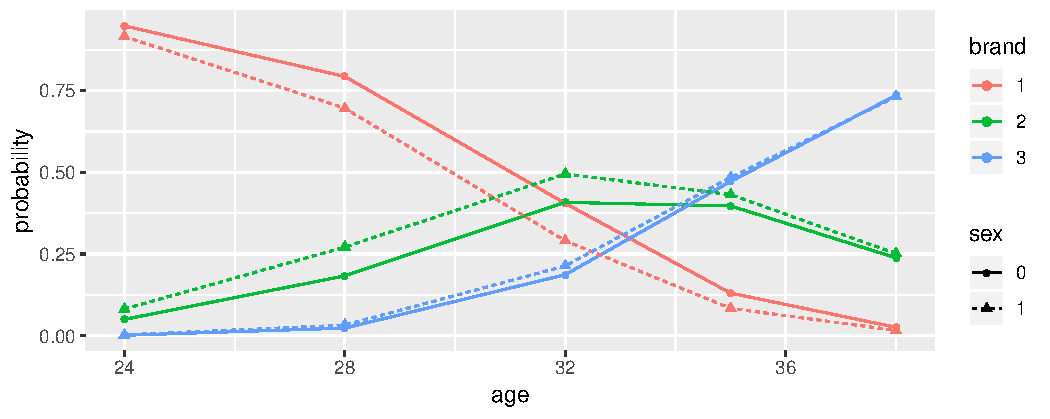
\includegraphics{figure/unnamed-chunk-116-1.pdf}
\caption{plot of chunk unnamed-chunk-116}
\end{figure}

\end{frame}

\begin{frame}{Digesting the plot}
\protect\hypertarget{digesting-the-plot}{}

\begin{itemize}
\item
  Brand vs.~age: younger people (of both genders) prefer brand 1, but
  older people (of both genders) prefer brand 3. (Explains significant
  age effect.)
\item
  Brand vs.~sex: females (dashed) like brand 1 less than males (solid),
  like brand 2 more (for all ages).
\item
  Not much brand difference between genders (solid and dashed lines of
  same colours close), but enough to be significant.
\item
  Model didn't include interaction, so modelled effect of gender on
  brand same for each age, modelled effect of age same for each gender.
\end{itemize}

\end{frame}

\begin{frame}[fragile]{Alternative data format}
\protect\hypertarget{alternative-data-format}{}

Summarize all people of same brand preference, same sex, same age on one
line of data file with frequency on end:

\begin{verbatim}
1 0 24 1
1 0 26 2
1 0 27 4
1 0 28 4
1 0 29 7
1 0 30 3
...
\end{verbatim}

Whole data set in 65 lines not 735! But how?

\end{frame}

\begin{frame}[fragile]{Getting alternative data format}
\protect\hypertarget{getting-alternative-data-format}{}

\begin{Shaded}
\begin{Highlighting}[]
\NormalTok{brandpref }\OperatorTok
\StringTok{  }\KeywordTok{group_by}\NormalTok{(age, sex, brand) }\OperatorTok
\StringTok{  }\KeywordTok{summarize}\NormalTok{(}\DataTypeTok{Freq =} \KeywordTok{n}\NormalTok{()) }\OperatorTok
\StringTok{  }\KeywordTok{ungroup}\NormalTok{() ->}\StringTok{ }\NormalTok{b}
\NormalTok{b }\OperatorTok\StringTok{ }\KeywordTok{slice}\NormalTok{(}\DecValTok{1}\OperatorTok{:}\DecValTok{6}\NormalTok{)}
\end{Highlighting}
\end{Shaded}

\begin{verbatim}
## # A tibble: 6 x 4
##     age sex   brand  Freq
##   <dbl> <fct> <fct> <int>
## 1    24 0     1         1
## 2    26 0     1         2
## 3    27 0     1         4
## 4    27 1     1         4
## 5    27 1     3         1
## 6    28 0     1         4
\end{verbatim}

\end{frame}

\begin{frame}[fragile]{Fitting models, almost the same}
\protect\hypertarget{fitting-models-almost-the-same}{}

\begin{itemize}
\item
  Just have to remember \texttt{weights} to incorporate frequencies.
\item
  Otherwise \texttt{multinom} assumes you have just 1 obs on each line!
\item
  Again turn (numerical) \texttt{sex} and \texttt{brand} into factors:
\end{itemize}

\footnotesize

\begin{Shaded}
\begin{Highlighting}[]
\NormalTok{b }\OperatorTok
\StringTok{  }\KeywordTok{mutate}\NormalTok{(}\DataTypeTok{sex =} \KeywordTok{factor}\NormalTok{(sex)) }\OperatorTok
\StringTok{  }\KeywordTok{mutate}\NormalTok{(}\DataTypeTok{brand =} \KeywordTok{factor}\NormalTok{(brand)) ->}\StringTok{ }\NormalTok{bf}
\NormalTok{b}\FloatTok{.1}\NormalTok{ <-}\StringTok{ }\KeywordTok{multinom}\NormalTok{(brand }\OperatorTok{~}\StringTok{ }\NormalTok{age }\OperatorTok{+}\StringTok{ }\NormalTok{sex, }\DataTypeTok{data =}\NormalTok{ bf, }\DataTypeTok{weights =}\NormalTok{ Freq)}
\NormalTok{b}\FloatTok{.2}\NormalTok{ <-}\StringTok{ }\KeywordTok{multinom}\NormalTok{(brand }\OperatorTok{~}\StringTok{ }\NormalTok{age, }\DataTypeTok{data =}\NormalTok{ bf, }\DataTypeTok{weights =}\NormalTok{ Freq)}
\end{Highlighting}
\end{Shaded}

\normalsize

\end{frame}

\begin{frame}[fragile]{P-value for \texttt{sex} identical}
\protect\hypertarget{p-value-for-sex-identical}{}

\footnotesize

\begin{Shaded}
\begin{Highlighting}[]
\KeywordTok{anova}\NormalTok{(b}\FloatTok{.2}\NormalTok{, b}\FloatTok{.1}\NormalTok{)}
\end{Highlighting}
\end{Shaded}

\begin{verbatim}
## Likelihood ratio tests of Multinomial Models
## 
## Response: brand
##       Model Resid. df Resid. Dev   Test    Df LR stat.    Pr(Chi)
## 1       age       126   1413.593                                 
## 2 age + sex       124   1405.941 1 vs 2     2 7.651236 0.02180495
\end{verbatim}

\normalsize

Same P-value as before, so we haven't changed anything important.

\end{frame}

\begin{frame}[fragile]{Including data on plot}
\protect\hypertarget{including-data-on-plot}{}

\begin{itemize}
\tightlist
\item
  Everyone's age given as whole number, so maybe not too many different
  ages with sensible amount of data at each:
\end{itemize}

\scriptsize

\begin{Shaded}
\begin{Highlighting}[]
\NormalTok{b }\OperatorTok
\StringTok{  }\KeywordTok{group_by}\NormalTok{(age) }\OperatorTok
\StringTok{  }\KeywordTok{summarize}\NormalTok{(}\DataTypeTok{total =} \KeywordTok{sum}\NormalTok{(Freq))}
\end{Highlighting}
\end{Shaded}

\begin{verbatim}
## # A tibble: 14 x 2
##      age total
##    <dbl> <int>
##  1    24     1
##  2    26     2
##  3    27     9
##  4    28    15
##  5    29    19
##  6    30    23
##  7    31    40
##  8    32   333
##  9    33    55
## 10    34    64
## 11    35    35
## 12    36    85
## 13    37    22
## 14    38    32
\end{verbatim}

\normalsize

\end{frame}

\begin{frame}[fragile]{Comments and next}
\protect\hypertarget{comments-and-next}{}

\begin{itemize}
\item
  Not great (especially at low end), but live with it.
\item
  Need proportions of frequencies in each brand for each age-gender
  combination. Mimic what we did for miners:
\end{itemize}

\begin{Shaded}
\begin{Highlighting}[]
\NormalTok{b }\OperatorTok
\StringTok{  }\KeywordTok{group_by}\NormalTok{(age, sex) }\OperatorTok
\StringTok{  }\KeywordTok{mutate}\NormalTok{(}\DataTypeTok{proportion =}\NormalTok{ Freq }\OperatorTok{/}\StringTok{ }\KeywordTok{sum}\NormalTok{(Freq)) ->}\StringTok{ }\NormalTok{brands}
\end{Highlighting}
\end{Shaded}

\end{frame}

\begin{frame}[fragile]{Checking proportions for age 32}
\protect\hypertarget{checking-proportions-for-age-32}{}

\small

\begin{Shaded}
\begin{Highlighting}[]
\NormalTok{brands }\OperatorTok\StringTok{ }\KeywordTok{filter}\NormalTok{(age }\OperatorTok{==}\StringTok{ }\DecValTok{32}\NormalTok{)}
\end{Highlighting}
\end{Shaded}

\begin{verbatim}
## # A tibble: 6 x 5
## # Groups:   age, sex [2]
##     age sex   brand  Freq proportion
##   <dbl> <fct> <fct> <int>      <dbl>
## 1    32 0     1        48      0.407
## 2    32 0     2        51      0.432
## 3    32 0     3        19      0.161
## 4    32 1     1        62      0.288
## 5    32 1     2       117      0.544
## 6    32 1     3        36      0.167
\end{verbatim}

\normalsize

\begin{itemize}
\item
  First three proportions (males) add up to 1.
\item
  Last three proportions (females) add up to 1.
\item
  So looks like proportions of right thing.
\end{itemize}

\end{frame}

\begin{frame}[fragile]{Attempting plot}
\protect\hypertarget{attempting-plot}{}

\begin{itemize}
\item
  Take code from previous plot and:
\item
  remove \texttt{geom\_point} for fitted values
\item
  add \texttt{geom\_point} with correct \texttt{data=} and \texttt{aes}
  to plot data.
\end{itemize}

\begin{Shaded}
\begin{Highlighting}[]
\NormalTok{g <-}\StringTok{ }\KeywordTok{ggplot}\NormalTok{(probs.long, }\KeywordTok{aes}\NormalTok{(}
  \DataTypeTok{x =}\NormalTok{ age, }\DataTypeTok{y =}\NormalTok{ probability,}
  \DataTypeTok{colour =}\NormalTok{ brand, }\DataTypeTok{shape =}\NormalTok{ sex}
\NormalTok{)) }\OperatorTok{+}
\StringTok{  }\KeywordTok{geom_line}\NormalTok{(}\KeywordTok{aes}\NormalTok{(}\DataTypeTok{linetype =}\NormalTok{ sex)) }\OperatorTok{+}
\StringTok{  }\KeywordTok{geom_point}\NormalTok{(}\DataTypeTok{data =}\NormalTok{ brands, }\KeywordTok{aes}\NormalTok{(}\DataTypeTok{y =}\NormalTok{ proportion))}
\end{Highlighting}
\end{Shaded}

\begin{itemize}
\tightlist
\item
  Data seem to correspond more or less to fitted curves:
\end{itemize}

\end{frame}

\begin{frame}[fragile]{The plot}
\protect\hypertarget{the-plot-2}{}

\begin{Shaded}
\begin{Highlighting}[]
\NormalTok{g}
\end{Highlighting}
\end{Shaded}

\begin{figure}
\centering
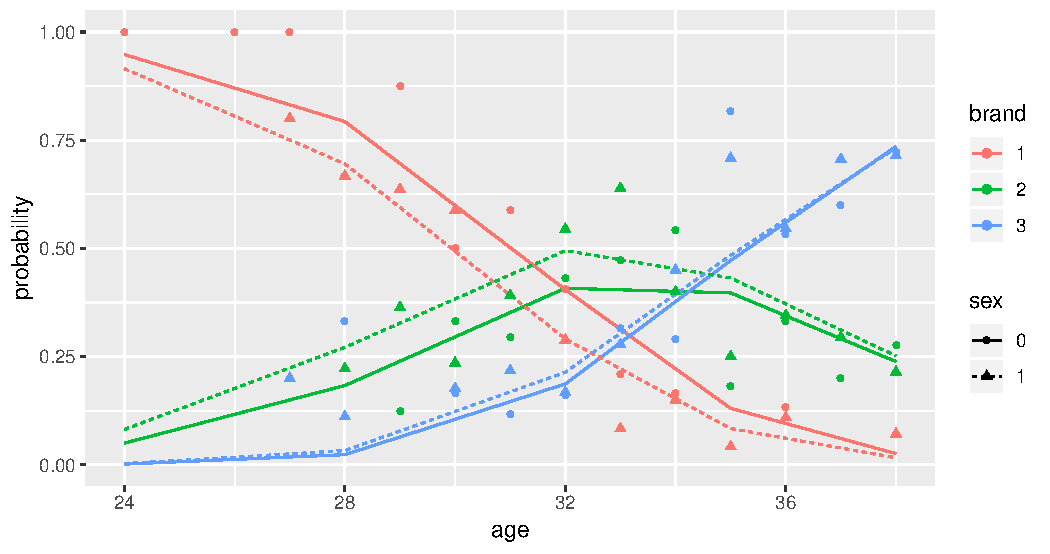
\includegraphics{figure/unnamed-chunk-123-1.pdf}
\caption{plot of chunk unnamed-chunk-123}
\end{figure}

\end{frame}

\begin{frame}[fragile]{But\ldots}
\protect\hypertarget{but-1}{}

\begin{itemize}
\item
  Some of the plotted points based on a lot of people, and some only a
  few.
\item
  Idea: make the \emph{size} of plotted point bigger if point based on a
  lot of people (in \texttt{Freq}).
\item
  Hope that larger points then closer to predictions.
\item
  Code:
\end{itemize}

\footnotesize

\begin{Shaded}
\begin{Highlighting}[]
\NormalTok{g <-}\StringTok{ }\KeywordTok{ggplot}\NormalTok{(probs.long, }\KeywordTok{aes}\NormalTok{(}
  \DataTypeTok{x =}\NormalTok{ age, }\DataTypeTok{y =}\NormalTok{ probability,}
  \DataTypeTok{colour =}\NormalTok{ brand, }\DataTypeTok{shape =}\NormalTok{ sex}
\NormalTok{)) }\OperatorTok{+}
\StringTok{  }\KeywordTok{geom_line}\NormalTok{(}\KeywordTok{aes}\NormalTok{(}\DataTypeTok{linetype =}\NormalTok{ sex)) }\OperatorTok{+}
\StringTok{  }\KeywordTok{geom_point}\NormalTok{(}
    \DataTypeTok{data =}\NormalTok{ brands,}
    \KeywordTok{aes}\NormalTok{(}\DataTypeTok{y =}\NormalTok{ proportion, }\DataTypeTok{size =}\NormalTok{ Freq)}
\NormalTok{  )}
\end{Highlighting}
\end{Shaded}

\normalsize

\end{frame}

\begin{frame}[fragile]{The plot}
\protect\hypertarget{the-plot-3}{}

\begin{Shaded}
\begin{Highlighting}[]
\NormalTok{g}
\end{Highlighting}
\end{Shaded}

\begin{figure}
\centering
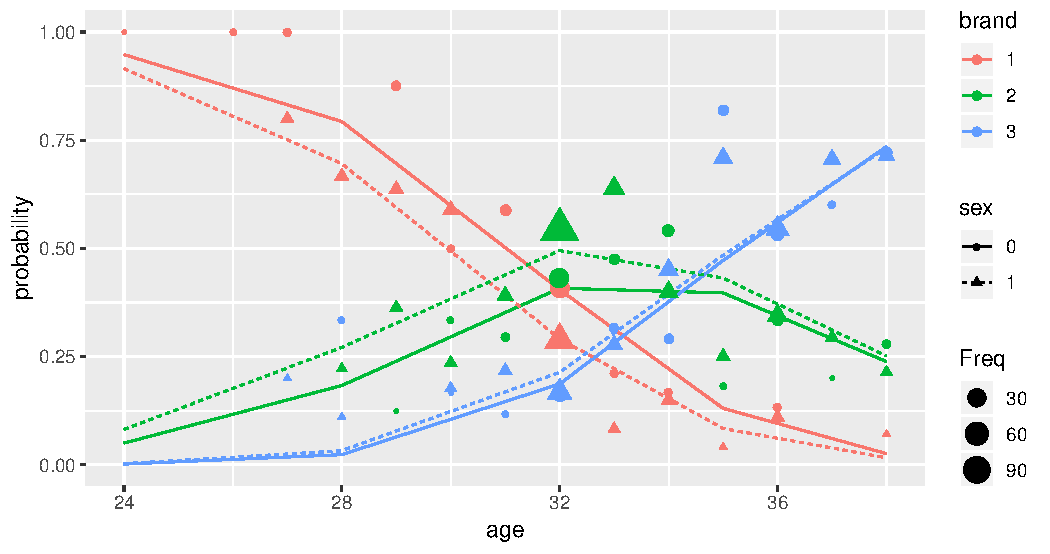
\includegraphics{figure/unnamed-chunk-125-1.pdf}
\caption{plot of chunk unnamed-chunk-125}
\end{figure}

\end{frame}

\begin{frame}[fragile]{Trying interaction between age and gender}
\protect\hypertarget{trying-interaction-between-age-and-gender}{}

\scriptsize

\begin{Shaded}
\begin{Highlighting}[]
\NormalTok{b}\FloatTok{.4}\NormalTok{ <-}\StringTok{ }\KeywordTok{update}\NormalTok{(b}\FloatTok{.1}\NormalTok{, . }\OperatorTok{~}\StringTok{ }\NormalTok{. }\OperatorTok{+}\StringTok{ }\NormalTok{age}\OperatorTok{:}\NormalTok{sex)}
\end{Highlighting}
\end{Shaded}

\begin{verbatim}
## # weights:  15 (8 variable)
## initial  value 807.480032 
## iter  10 value 704.811229
## iter  20 value 702.582802
## final  value 702.582761 
## converged
\end{verbatim}

\begin{Shaded}
\begin{Highlighting}[]
\KeywordTok{anova}\NormalTok{(b}\FloatTok{.1}\NormalTok{, b}\FloatTok{.4}\NormalTok{)}
\end{Highlighting}
\end{Shaded}

\begin{verbatim}
## Likelihood ratio tests of Multinomial Models
## 
## Response: brand
##                 Model Resid. df Resid. Dev   Test    Df
## 1           age + sex       124   1405.941             
## 2 age + sex + age:sex       122   1405.166 1 vs 2     2
##    LR stat.  Pr(Chi)
## 1                   
## 2 0.7758861 0.678451
\end{verbatim}

\normalsize

\begin{itemize}
\tightlist
\item
  No evidence that effect of age on brand preference differs for the two
  genders.
\end{itemize}

\end{frame}

\hypertarget{survival-analysis}{%
\section{Survival analysis}\label{survival-analysis}}

\begin{frame}{Survival analysis}
\protect\hypertarget{survival-analysis-1}{}

\begin{itemize}
\item
  So far, have seen:

  \begin{itemize}
  \item
    response variable counted or measured (regression)
  \item
    response variable categorized (logistic regression)
  \end{itemize}
\end{itemize}

and have predicted response from explanatory variables.

\begin{itemize}
\item
  But what if response is time until event (eg. time of survival after
  surgery)?
\item
  Additional complication: event might not have happened at end of study
  (eg. patient still alive). But knowing that patient has ``not died
  yet'' presumably informative. Such data called \emph{censored}.
\item
  Enter \emph{survival analysis}, in particular the ``Cox proportional
  hazards model''.
\item
  Explanatory variables in this context often called \emph{covariates}.
\end{itemize}

\end{frame}

\begin{frame}{Example: still dancing?}
\protect\hypertarget{example-still-dancing}{}

\begin{itemize}
\item
  12 women who have just started taking dancing lessons are followed for
  up to a year, to see whether they are still taking dancing lessons, or
  have quit. The ``event'' here is ``quit''.
\item
  This might depend on:

  \begin{itemize}
  \item
    a treatment (visit to a dance competition)
  \item
    woman's age (at start of study).
  \end{itemize}
\end{itemize}

\end{frame}

\begin{frame}[fragile]{Data}
\protect\hypertarget{data}{}

\normalsize

\begin{verbatim}
Months  Quit   Treatment Age
1        1        0      16
2        1        0      24
2        1        0      18
3        0        0      27
4        1        0      25
7        1        1      26
8        1        1      36
10       1        1      38
10       0        1      45
12       1        1      47
\end{verbatim}

\normalsize

\end{frame}

\begin{frame}[fragile]{About the data}
\protect\hypertarget{about-the-data}{}

\begin{itemize}
\item
  \texttt{months} and \texttt{quit} are kind of combined response:

  \begin{itemize}
  \item
    \texttt{Months} is number of months a woman was actually observed
    dancing
  \item
    \texttt{quit} is 1 if woman quit, 0 if still dancing at end of
    study.
  \end{itemize}
\item
  Treatment is 1 if woman went to dance competition, 0 otherwise.
\item
  Fit model and see whether \texttt{Age} or \texttt{Treatment} have
  effect on survival.
\item
  Want to do predictions for probabilities of still dancing as they
  depend on whatever is significant, and draw plot.
\end{itemize}

\end{frame}

\begin{frame}[fragile]{Packages (for this section)}
\protect\hypertarget{packages-for-this-section}{}

\begin{itemize}
\item
  Install packages \texttt{survival} and \texttt{survminer} if not done.
\item
  Load \texttt{survival}, \texttt{survminer}, \texttt{broom} and
  \texttt{tidyverse}:
\end{itemize}

\begin{Shaded}
\begin{Highlighting}[]
\KeywordTok{library}\NormalTok{(tidyverse)}
\KeywordTok{library}\NormalTok{(survival)}
\KeywordTok{library}\NormalTok{(survminer)}
\KeywordTok{library}\NormalTok{(broom)}
\end{Highlighting}
\end{Shaded}

\end{frame}

\begin{frame}[fragile]{Read data}
\protect\hypertarget{read-data}{}

\begin{itemize}
\tightlist
\item
  Column-aligned:
\end{itemize}

\normalsize

\begin{Shaded}
\begin{Highlighting}[]
\NormalTok{url <-}\StringTok{ "http://www.utsc.utoronto.ca/~butler/d29/dancing.txt"}
\NormalTok{dance <-}\StringTok{ }\KeywordTok{read_table}\NormalTok{(url)}
\end{Highlighting}
\end{Shaded}

\begin{verbatim}
## Parsed with column specification:
## cols(
##   Months = col_double(),
##   Quit = col_double(),
##   Treatment = col_double(),
##   Age = col_double()
## )
\end{verbatim}

\normalsize

\end{frame}

\begin{frame}[fragile]{The data}
\protect\hypertarget{the-data-5}{}

\small

\begin{Shaded}
\begin{Highlighting}[]
\NormalTok{dance}
\end{Highlighting}
\end{Shaded}

\begin{verbatim}
## # A tibble: 12 x 4
##    Months  Quit Treatment   Age
##     <dbl> <dbl>     <dbl> <dbl>
##  1      1     1         0    16
##  2      2     1         0    24
##  3      2     1         0    18
##  4      3     0         0    27
##  5      4     1         0    25
##  6      5     1         0    21
##  7     11     1         0    55
##  8      7     1         1    26
##  9      8     1         1    36
## 10     10     1         1    38
## 11     10     0         1    45
## 12     12     1         1    47
\end{verbatim}

\normalsize

\end{frame}

\begin{frame}[fragile]{Examine response and fit model}
\protect\hypertarget{examine-response-and-fit-model}{}

\begin{itemize}
\tightlist
\item
  Response variable (has to be outside data frame):
\end{itemize}

\small

\begin{Shaded}
\begin{Highlighting}[]
\NormalTok{mth <-}\StringTok{ }\KeywordTok{with}\NormalTok{(dance, }\KeywordTok{Surv}\NormalTok{(Months, Quit))}
\NormalTok{mth}
\end{Highlighting}
\end{Shaded}

\begin{verbatim}
##  [1]  1   2   2   3+  4   5  11   7   8  10  10+ 12
\end{verbatim}

\normalsize

\begin{itemize}
\tightlist
\item
  Then fit model, predicting \texttt{mth} from explanatories:
\end{itemize}

\begin{Shaded}
\begin{Highlighting}[]
\NormalTok{dance}\FloatTok{.1}\NormalTok{ <-}\StringTok{ }\KeywordTok{coxph}\NormalTok{(mth }\OperatorTok{~}\StringTok{ }\NormalTok{Treatment }\OperatorTok{+}\StringTok{ }\NormalTok{Age, }\DataTypeTok{data =}\NormalTok{ dance)}
\end{Highlighting}
\end{Shaded}

\end{frame}

\begin{frame}[fragile]{Output looks a lot like regression}
\protect\hypertarget{output-looks-a-lot-like-regression}{}

\scriptsize

\begin{Shaded}
\begin{Highlighting}[]
\KeywordTok{summary}\NormalTok{(dance}\FloatTok{.1}\NormalTok{)}
\end{Highlighting}
\end{Shaded}

\begin{verbatim}
## Call:
## coxph(formula = mth ~ Treatment + Age, data = dance)
## 
##   n= 12, number of events= 10 
## 
##               coef exp(coef) se(coef)      z Pr(>|z|)  
## Treatment -4.44915   0.01169  2.60929 -1.705   0.0882 .
## Age       -0.36619   0.69337  0.15381 -2.381   0.0173 *
## ---
## Signif. codes:  
## 0 '***' 0.001 '**' 0.01 '*' 0.05 '.' 0.1 ' ' 1
## 
##           exp(coef) exp(-coef) lower .95 upper .95
## Treatment   0.01169     85.554 7.026e-05    1.9444
## Age         0.69337      1.442 5.129e-01    0.9373
## 
## Concordance= 0.964  (se = 0.039 )
## Likelihood ratio test= 21.68  on 2 df,   p=2e-05
## Wald test            = 5.67  on 2 df,   p=0.06
## Score (logrank) test = 14.75  on 2 df,   p=6e-04
\end{verbatim}

\normalsize

\end{frame}

\begin{frame}[fragile]{Conclusions}
\protect\hypertarget{conclusions-1}{}

\begin{itemize}
\item
  Use \(\alpha=0.10\) here since not much data.
\item
  Three tests at bottom like global F-test. Consensus that something
  predicts survival time (whether or not dancer quit and how long it
  took).
\item
  \texttt{Age} (definitely), \texttt{Treatment} (marginally) both
  predict survival time.
\end{itemize}

\end{frame}

\begin{frame}[fragile]{Model checking}
\protect\hypertarget{model-checking}{}

\begin{itemize}
\item
  With regression, usually plot residuals against fitted values.
\item
  Not quite same here (nonlinear model), but ``martingale residuals''
  should have no pattern vs.~``linear predictor''.
\item
  \texttt{ggcoxdiagnostics} from package \texttt{survminer} makes plot,
  to which we add smooth. If smooth trend more or less straight across,
  model OK.
\item
  Martingale residuals can go very negative, so won't always look
  normal.
\end{itemize}

\end{frame}

\begin{frame}[fragile]{Martingale residual plot for dance data}
\protect\hypertarget{martingale-residual-plot-for-dance-data}{}

This looks good (with only 12 points):

\begin{Shaded}
\begin{Highlighting}[]
\KeywordTok{ggcoxdiagnostics}\NormalTok{(dance}\FloatTok{.1}\NormalTok{) }\OperatorTok{+}\StringTok{ }\KeywordTok{geom_smooth}\NormalTok{(}\DataTypeTok{se =}\NormalTok{ F)}
\end{Highlighting}
\end{Shaded}

\begin{verbatim}
## `geom_smooth()` using method = 'loess' and formula 'y ~ x'
\end{verbatim}

\begin{figure}
\centering
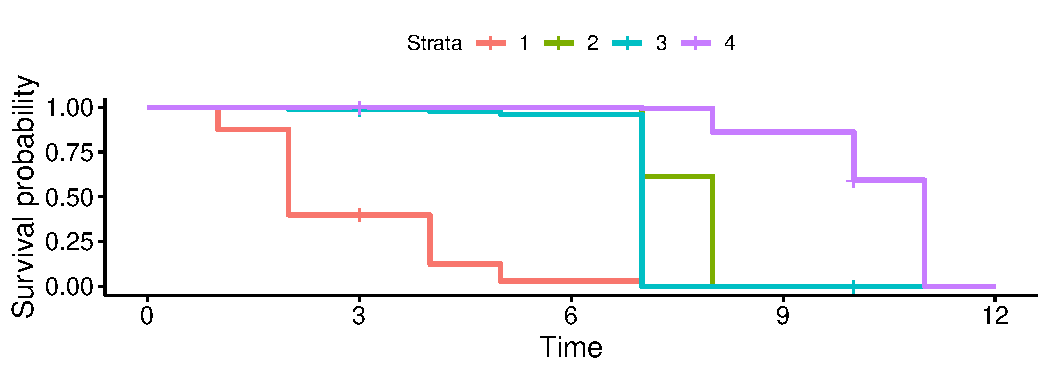
\includegraphics{figure/unnamed-chunk-134-1.pdf}
\caption{plot of chunk unnamed-chunk-134}
\end{figure}

\end{frame}

\begin{frame}[fragile]{Predicted survival probs}
\protect\hypertarget{predicted-survival-probs-1}{}

\begin{itemize}
\tightlist
\item
  The function we use is called \texttt{survfit}, though actually works
  rather like \texttt{predict}.
\item
  First create a data frame of values to predict from. We'll do all
  combos of ages 20 and 40, treatment and not, using \texttt{crossing}
  to get all the combos:
\end{itemize}

\small

\begin{Shaded}
\begin{Highlighting}[]
\NormalTok{treatments <-}\StringTok{ }\KeywordTok{c}\NormalTok{(}\DecValTok{0}\NormalTok{, }\DecValTok{1}\NormalTok{)}
\NormalTok{ages <-}\StringTok{ }\KeywordTok{c}\NormalTok{(}\DecValTok{20}\NormalTok{, }\DecValTok{40}\NormalTok{)}
\NormalTok{dance.new <-}\StringTok{ }\KeywordTok{crossing}\NormalTok{(}\DataTypeTok{Treatment =}\NormalTok{ treatments, }\DataTypeTok{Age =}\NormalTok{ ages)}
\NormalTok{dance.new}
\end{Highlighting}
\end{Shaded}

\begin{verbatim}
## # A tibble: 4 x 2
##   Treatment   Age
##       <dbl> <dbl>
## 1         0    20
## 2         0    40
## 3         1    20
## 4         1    40
\end{verbatim}

\normalsize

\end{frame}

\begin{frame}[fragile]{The predictions}
\protect\hypertarget{the-predictions-1}{}

One prediction \emph{for each time} for each combo of age and treatment
in \texttt{dance.new}:

\footnotesize

\begin{Shaded}
\begin{Highlighting}[]
\NormalTok{s <-}\StringTok{ }\KeywordTok{survfit}\NormalTok{(dance}\FloatTok{.1}\NormalTok{, }\DataTypeTok{newdata =}\NormalTok{ dance.new, }\DataTypeTok{data =}\NormalTok{ dance)}
\KeywordTok{summary}\NormalTok{(s)}
\end{Highlighting}
\end{Shaded}

\begin{verbatim}
## Call: survfit(formula = dance.1, newdata = dance.new, data = dance)
## 
##  time n.risk n.event survival1 survival2 survival3 survival4
##     1     12       1  8.76e-01  1.00e+00  9.98e-01     1.000
##     2     11       2  3.99e-01  9.99e-01  9.89e-01     1.000
##     4      8       1  1.24e-01  9.99e-01  9.76e-01     1.000
##     5      7       1  2.93e-02  9.98e-01  9.60e-01     1.000
##     7      6       1 2.96e-323  6.13e-01  1.70e-04     0.994
##     8      5       1  0.00e+00  2.99e-06  1.35e-98     0.862
##    10      4       1  0.00e+00  3.61e-20  0.00e+00     0.593
##    11      2       1  0.00e+00  0.00e+00  0.00e+00     0.000
##    12      1       1  0.00e+00  0.00e+00  0.00e+00     0.000
\end{verbatim}

\normalsize

\end{frame}

\begin{frame}[fragile]{Conclusions from predicted probs}
\protect\hypertarget{conclusions-from-predicted-probs}{}

\begin{itemize}
\item
  Older women more likely to be still dancing than younger women
  (compare ``profiles'' for same treatment group).
\item
  Effect of treatment seems to be to increase prob of still dancing
  (compare ``profiles'' for same age for treatment group vs.~not)
\item
  Would be nice to see this on a graph. This is \texttt{ggsurvplot} from
  package \texttt{survminer}:
\end{itemize}

\begin{Shaded}
\begin{Highlighting}[]
\NormalTok{g <-}\StringTok{ }\KeywordTok{ggsurvplot}\NormalTok{(s, }\DataTypeTok{conf.int =}\NormalTok{ F)}
\end{Highlighting}
\end{Shaded}

\begin{itemize}
\tightlist
\item
  uses ``strata'' thus (\texttt{dance.new}):
\end{itemize}

\footnotesize

\begin{verbatim}
## # A tibble: 4 x 2
##   Treatment   Age
##       <dbl> <dbl>
## 1         0    20
## 2         0    40
## 3         1    20
## 4         1    40
\end{verbatim}

\normalsize

\end{frame}

\begin{frame}[fragile]{Plotting survival probabilities}
\protect\hypertarget{plotting-survival-probabilities}{}

\begin{Shaded}
\begin{Highlighting}[]
\NormalTok{g}
\end{Highlighting}
\end{Shaded}

\begin{figure}
\centering
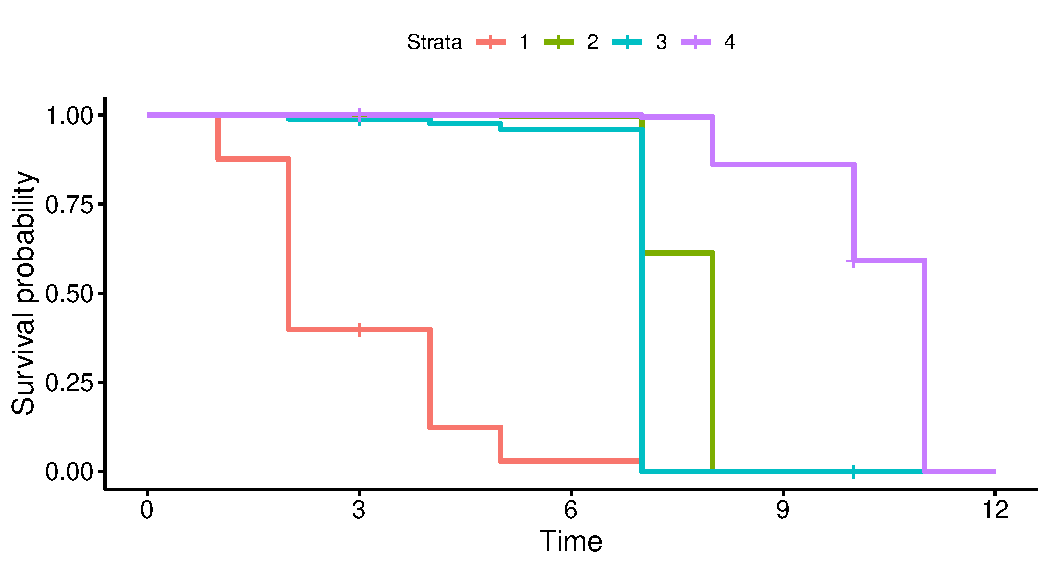
\includegraphics{figure/survival-plot-1.pdf}
\caption{plot of chunk survival-plot}
\end{figure}

\end{frame}

\begin{frame}{Discussion}
\protect\hypertarget{discussion}{}

\begin{itemize}
\item
  Survivor curve farther to the right is better (better chance of
  surviving longer).
\item
  Best is age 40 with treatment, worst age 20 without.
\item
  Appears to be:

  \begin{itemize}
  \item
    age effect (40 better than 20)
  \item
    treatment effect (treatment better than not)
  \item
    In analysis, treatment effect only marginally significant.
  \end{itemize}
\end{itemize}

\end{frame}

\begin{frame}[fragile]{A more realistic example: lung cancer}
\protect\hypertarget{a-more-realistic-example-lung-cancer}{}

\begin{itemize}
\item
  When you load in an R package, get data sets to illustrate functions
  in the package.
\item
  One such is \texttt{lung}. Data set measuring survival in patients
  with advanced lung cancer.
\item
  Along with survival time, number of ``performance scores'' included,
  measuring how well patients can perform daily activities.
\item
  Sometimes high good, but sometimes bad!
\item
  Variables below, from the data set help file (\texttt{?lung}).
\end{itemize}

\end{frame}

\begin{frame}{The variables}
\protect\hypertarget{the-variables}{}

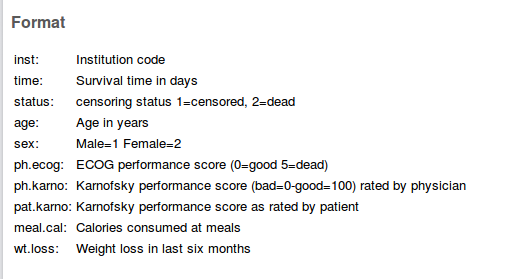
\includegraphics{lung-cancer-data.png}

\end{frame}

\begin{frame}[fragile]{Uh oh, missing values}
\protect\hypertarget{uh-oh-missing-values}{}

\scriptsize

\begin{Shaded}
\begin{Highlighting}[]
\NormalTok{lung }\OperatorTok\StringTok{ }\KeywordTok{slice}\NormalTok{(}\DecValTok{1}\OperatorTok{:}\DecValTok{16}\NormalTok{)}
\end{Highlighting}
\end{Shaded}

\begin{verbatim}
##    inst time status age sex ph.ecog ph.karno pat.karno meal.cal wt.loss
## 1     3  306      2  74   1       1       90       100     1175      NA
## 2     3  455      2  68   1       0       90        90     1225      15
## 3     3 1010      1  56   1       0       90        90       NA      15
## 4     5  210      2  57   1       1       90        60     1150      11
## 5     1  883      2  60   1       0      100        90       NA       0
## 6    12 1022      1  74   1       1       50        80      513       0
## 7     7  310      2  68   2       2       70        60      384      10
## 8    11  361      2  71   2       2       60        80      538       1
## 9     1  218      2  53   1       1       70        80      825      16
## 10    7  166      2  61   1       2       70        70      271      34
## 11    6  170      2  57   1       1       80        80     1025      27
## 12   16  654      2  68   2       2       70        70       NA      23
## 13   11  728      2  68   2       1       90        90       NA       5
## 14   21   71      2  60   1      NA       60        70     1225      32
## 15   12  567      2  57   1       1       80        70     2600      60
## 16    1  144      2  67   1       1       80        90       NA      15
\end{verbatim}

\normalsize

\end{frame}

\begin{frame}[fragile]{A closer look}
\protect\hypertarget{a-closer-look}{}

\tiny

\begin{Shaded}
\begin{Highlighting}[]
\KeywordTok{summary}\NormalTok{(lung)}
\end{Highlighting}
\end{Shaded}

\begin{verbatim}
##       inst            time            status           age             sex       
##  Min.   : 1.00   Min.   :   5.0   Min.   :1.000   Min.   :39.00   Min.   :1.000  
##  1st Qu.: 3.00   1st Qu.: 166.8   1st Qu.:1.000   1st Qu.:56.00   1st Qu.:1.000  
##  Median :11.00   Median : 255.5   Median :2.000   Median :63.00   Median :1.000  
##  Mean   :11.09   Mean   : 305.2   Mean   :1.724   Mean   :62.45   Mean   :1.395  
##  3rd Qu.:16.00   3rd Qu.: 396.5   3rd Qu.:2.000   3rd Qu.:69.00   3rd Qu.:2.000  
##  Max.   :33.00   Max.   :1022.0   Max.   :2.000   Max.   :82.00   Max.   :2.000  
##  NA's   :1                                                                       
##     ph.ecog          ph.karno        pat.karno         meal.cal         wt.loss       
##  Min.   :0.0000   Min.   : 50.00   Min.   : 30.00   Min.   :  96.0   Min.   :-24.000  
##  1st Qu.:0.0000   1st Qu.: 75.00   1st Qu.: 70.00   1st Qu.: 635.0   1st Qu.:  0.000  
##  Median :1.0000   Median : 80.00   Median : 80.00   Median : 975.0   Median :  7.000  
##  Mean   :0.9515   Mean   : 81.94   Mean   : 79.96   Mean   : 928.8   Mean   :  9.832  
##  3rd Qu.:1.0000   3rd Qu.: 90.00   3rd Qu.: 90.00   3rd Qu.:1150.0   3rd Qu.: 15.750  
##  Max.   :3.0000   Max.   :100.00   Max.   :100.00   Max.   :2600.0   Max.   : 68.000  
##  NA's   :1        NA's   :1        NA's   :3        NA's   :47       NA's   :14
\end{verbatim}

\normalsize

\end{frame}

\begin{frame}[fragile]{Remove obs with \emph{any} missing values}
\protect\hypertarget{remove-obs-with-any-missing-values}{}

\small

\begin{Shaded}
\begin{Highlighting}[]
\NormalTok{lung }\OperatorTok\StringTok{ }\KeywordTok{drop_na}\NormalTok{() ->}\StringTok{ }\NormalTok{lung.complete}
\NormalTok{lung.complete }\OperatorTok
\StringTok{  }\KeywordTok{select}\NormalTok{(meal.cal}\OperatorTok{:}\NormalTok{wt.loss) }\OperatorTok
\StringTok{  }\KeywordTok{slice}\NormalTok{(}\DecValTok{1}\OperatorTok{:}\DecValTok{10}\NormalTok{)}
\end{Highlighting}
\end{Shaded}

\begin{verbatim}
##    meal.cal wt.loss
## 1      1225      15
## 2      1150      11
## 3       513       0
## 4       384      10
## 5       538       1
## 6       825      16
## 7       271      34
## 8      1025      27
## 9      2600      60
## 10     1150      -5
\end{verbatim}

\normalsize

Missing values seem to be gone.

\end{frame}

\begin{frame}[fragile]{Check!}
\protect\hypertarget{check}{}

\tiny

\begin{Shaded}
\begin{Highlighting}[]
\KeywordTok{summary}\NormalTok{(lung.complete)}
\end{Highlighting}
\end{Shaded}

\begin{verbatim}
##       inst            time            status           age             sex       
##  Min.   : 1.00   Min.   :   5.0   Min.   :1.000   Min.   :39.00   Min.   :1.000  
##  1st Qu.: 3.00   1st Qu.: 174.5   1st Qu.:1.000   1st Qu.:57.00   1st Qu.:1.000  
##  Median :11.00   Median : 268.0   Median :2.000   Median :64.00   Median :1.000  
##  Mean   :10.71   Mean   : 309.9   Mean   :1.719   Mean   :62.57   Mean   :1.383  
##  3rd Qu.:15.00   3rd Qu.: 419.5   3rd Qu.:2.000   3rd Qu.:70.00   3rd Qu.:2.000  
##  Max.   :32.00   Max.   :1022.0   Max.   :2.000   Max.   :82.00   Max.   :2.000  
##     ph.ecog          ph.karno        pat.karno         meal.cal         wt.loss       
##  Min.   :0.0000   Min.   : 50.00   Min.   : 30.00   Min.   :  96.0   Min.   :-24.000  
##  1st Qu.:0.0000   1st Qu.: 70.00   1st Qu.: 70.00   1st Qu.: 619.0   1st Qu.:  0.000  
##  Median :1.0000   Median : 80.00   Median : 80.00   Median : 975.0   Median :  7.000  
##  Mean   :0.9581   Mean   : 82.04   Mean   : 79.58   Mean   : 929.1   Mean   :  9.719  
##  3rd Qu.:1.0000   3rd Qu.: 90.00   3rd Qu.: 90.00   3rd Qu.:1162.5   3rd Qu.: 15.000  
##  Max.   :3.0000   Max.   :100.00   Max.   :100.00   Max.   :2600.0   Max.   : 68.000
\end{verbatim}

\normalsize

No missing values left.

\end{frame}

\begin{frame}[fragile]{Model 1: use everything except \texttt{inst}}
\protect\hypertarget{model-1-use-everything-except-inst}{}

\footnotesize

\begin{Shaded}
\begin{Highlighting}[]
\KeywordTok{names}\NormalTok{(lung.complete)}
\end{Highlighting}
\end{Shaded}

\begin{verbatim}
##  [1] "inst"      "time"      "status"    "age"       "sex"       "ph.ecog"   "ph.karno" 
##  [8] "pat.karno" "meal.cal"  "wt.loss"
\end{verbatim}

\normalsize

\begin{itemize}
\tightlist
\item
  Event was death, goes with \texttt{status} of 2:
\end{itemize}

\begin{Shaded}
\begin{Highlighting}[]
\NormalTok{resp <-}\StringTok{ }\KeywordTok{with}\NormalTok{(lung.complete, }\KeywordTok{Surv}\NormalTok{(time, status }\OperatorTok{==}\StringTok{ }\DecValTok{2}\NormalTok{))}
\NormalTok{lung}\FloatTok{.1}\NormalTok{ <-}\StringTok{ }\KeywordTok{coxph}\NormalTok{(resp }\OperatorTok{~}\StringTok{ }\NormalTok{. }\OperatorTok{-}\StringTok{ }\NormalTok{inst }\OperatorTok{-}\StringTok{ }\NormalTok{time }\OperatorTok{-}\StringTok{ }\NormalTok{status,}
  \DataTypeTok{data =}\NormalTok{ lung.complete}
\NormalTok{)}
\end{Highlighting}
\end{Shaded}

``Dot'' means ``all the other variables''.

\end{frame}

\begin{frame}[fragile]{\texttt{summary} of model 1: too tiny to see!}
\protect\hypertarget{summary-of-model-1-too-tiny-to-see}{}

\tiny

\begin{Shaded}
\begin{Highlighting}[]
\KeywordTok{summary}\NormalTok{(lung}\FloatTok{.1}\NormalTok{)}
\end{Highlighting}
\end{Shaded}

\begin{verbatim}
## Call:
## coxph(formula = resp ~ . - inst - time - status, data = lung.complete)
## 
##   n= 167, number of events= 120 
## 
##                 coef  exp(coef)   se(coef)      z Pr(>|z|)   
## age        1.080e-02  1.011e+00  1.160e-02  0.931  0.35168   
## sex       -5.536e-01  5.749e-01  2.016e-01 -2.746  0.00603 **
## ph.ecog    7.395e-01  2.095e+00  2.250e-01  3.287  0.00101 **
## ph.karno   2.244e-02  1.023e+00  1.123e-02  1.998  0.04575 * 
## pat.karno -1.207e-02  9.880e-01  8.116e-03 -1.488  0.13685   
## meal.cal   2.835e-05  1.000e+00  2.594e-04  0.109  0.91298   
## wt.loss   -1.420e-02  9.859e-01  7.766e-03 -1.828  0.06748 . 
## ---
## Signif. codes:  0 '***' 0.001 '**' 0.01 '*' 0.05 '.' 0.1 ' ' 1
## 
##           exp(coef) exp(-coef) lower .95 upper .95
## age          1.0109     0.9893    0.9881    1.0341
## sex          0.5749     1.7395    0.3872    0.8534
## ph.ecog      2.0950     0.4773    1.3479    3.2560
## ph.karno     1.0227     0.9778    1.0004    1.0455
## pat.karno    0.9880     1.0121    0.9724    1.0038
## meal.cal     1.0000     1.0000    0.9995    1.0005
## wt.loss      0.9859     1.0143    0.9710    1.0010
## 
## Concordance= 0.653  (se = 0.029 )
## Likelihood ratio test= 28.16  on 7 df,   p=2e-04
## Wald test            = 27.5  on 7 df,   p=3e-04
## Score (logrank) test = 28.31  on 7 df,   p=2e-04
\end{verbatim}

\normalsize

\end{frame}

\begin{frame}[fragile]{Overall significance}
\protect\hypertarget{overall-significance}{}

The three tests of overall significance: \small

\begin{Shaded}
\begin{Highlighting}[]
\KeywordTok{glance}\NormalTok{(lung}\FloatTok{.1}\NormalTok{) }\OperatorTok\StringTok{ }\KeywordTok{select}\NormalTok{(}\KeywordTok{starts_with}\NormalTok{(}\StringTok{"p.value"}\NormalTok{))}
\end{Highlighting}
\end{Shaded}

\begin{verbatim}
## # A tibble: 1 x 3
##   p.value.log p.value.sc p.value.wald
##         <dbl>      <dbl>        <dbl>
## 1    0.000205   0.000193     0.000271
\end{verbatim}

\normalsize

All strongly significant. \emph{Something} predicts survival.

\end{frame}

\begin{frame}[fragile]{Coefficients for model 1}
\protect\hypertarget{coefficients-for-model-1}{}

\small

\begin{Shaded}
\begin{Highlighting}[]
\KeywordTok{tidy}\NormalTok{(lung}\FloatTok{.1}\NormalTok{) }\OperatorTok\StringTok{ }\KeywordTok{select}\NormalTok{(term, p.value) }\OperatorTok\StringTok{ }\KeywordTok{arrange}\NormalTok{(p.value)}
\end{Highlighting}
\end{Shaded}

\begin{verbatim}
## # A tibble: 7 x 2
##   term      p.value
##   <chr>       <dbl>
## 1 ph.ecog   0.00101
## 2 sex       0.00603
## 3 ph.karno  0.0457 
## 4 wt.loss   0.0675 
## 5 pat.karno 0.137  
## 6 age       0.352  
## 7 meal.cal  0.913
\end{verbatim}

\normalsize

\begin{itemize}
\item
  \texttt{sex} and \texttt{ph.ecog} definitely significant here
\item
  \texttt{age}, \texttt{pat.karno} and \texttt{meal.cal} definitely not
\item
  Take out definitely non-sig variables, and try again.
\end{itemize}

\end{frame}

\begin{frame}[fragile]{Model 2}
\protect\hypertarget{model-2}{}

\normalsize

\begin{Shaded}
\begin{Highlighting}[]
\NormalTok{lung}\FloatTok{.2}\NormalTok{ <-}\StringTok{ }\KeywordTok{update}\NormalTok{(lung}\FloatTok{.1}\NormalTok{, . }\OperatorTok{~}\StringTok{ }\NormalTok{. }\OperatorTok{-}\StringTok{ }\NormalTok{age }\OperatorTok{-}\StringTok{ }\NormalTok{pat.karno }\OperatorTok{-}\StringTok{ }\NormalTok{meal.cal)}
\KeywordTok{tidy}\NormalTok{(lung}\FloatTok{.2}\NormalTok{) }\OperatorTok\StringTok{ }\KeywordTok{select}\NormalTok{(term, p.value)}
\end{Highlighting}
\end{Shaded}

\begin{verbatim}
## # A tibble: 4 x 2
##   term      p.value
##   <chr>       <dbl>
## 1 sex      0.00409 
## 2 ph.ecog  0.000112
## 3 ph.karno 0.101   
## 4 wt.loss  0.108
\end{verbatim}

\normalsize

\end{frame}

\begin{frame}[fragile]{Compare with first model:}
\protect\hypertarget{compare-with-first-model}{}

\normalsize

\begin{Shaded}
\begin{Highlighting}[]
\KeywordTok{anova}\NormalTok{(lung}\FloatTok{.2}\NormalTok{, lung}\FloatTok{.1}\NormalTok{)}
\end{Highlighting}
\end{Shaded}

\begin{verbatim}
## Analysis of Deviance Table
##  Cox model: response is  resp
##  Model 1: ~ sex + ph.ecog + ph.karno + wt.loss
##  Model 2: ~ (inst + time + status + age + sex + ph.ecog + ph.karno + pat.karno + meal.cal + wt.loss) - inst - time - status
##    loglik Chisq Df P(>|Chi|)
## 1 -495.67                   
## 2 -494.03 3.269  3     0.352
\end{verbatim}

\normalsize

\begin{itemize}
\tightlist
\item
  No harm in taking out those variables.
\end{itemize}

\end{frame}

\begin{frame}[fragile]{Model 3}
\protect\hypertarget{model-3}{}

Take out \texttt{ph.karno} and \texttt{wt.loss} as well.

\begin{Shaded}
\begin{Highlighting}[]
\NormalTok{lung}\FloatTok{.3}\NormalTok{ <-}\StringTok{ }\KeywordTok{update}\NormalTok{(lung}\FloatTok{.2}\NormalTok{, . }\OperatorTok{~}\StringTok{ }\NormalTok{. }\OperatorTok{-}\StringTok{ }\NormalTok{ph.karno }\OperatorTok{-}\StringTok{ }\NormalTok{wt.loss)}
\end{Highlighting}
\end{Shaded}

\begin{Shaded}
\begin{Highlighting}[]
\KeywordTok{tidy}\NormalTok{(lung}\FloatTok{.3}\NormalTok{) }\OperatorTok\StringTok{ }\KeywordTok{select}\NormalTok{(term, estimate, p.value)}
\end{Highlighting}
\end{Shaded}

\begin{verbatim}
## # A tibble: 2 x 3
##   term    estimate  p.value
##   <chr>      <dbl>    <dbl>
## 1 sex       -0.510 0.00958 
## 2 ph.ecog    0.483 0.000266
\end{verbatim}

\end{frame}

\begin{frame}[fragile]{Check whether that was OK}
\protect\hypertarget{check-whether-that-was-ok}{}

\begin{Shaded}
\begin{Highlighting}[]
\KeywordTok{anova}\NormalTok{(lung}\FloatTok{.3}\NormalTok{, lung}\FloatTok{.2}\NormalTok{)}
\end{Highlighting}
\end{Shaded}

\begin{verbatim}
## Analysis of Deviance Table
##  Cox model: response is  resp
##  Model 1: ~ sex + ph.ecog
##  Model 2: ~ sex + ph.ecog + ph.karno + wt.loss
##    loglik  Chisq Df P(>|Chi|)  
## 1 -498.38                      
## 2 -495.67 5.4135  2   0.06675 .
## ---
## Signif. codes:  0 '***' 0.001 '**' 0.01 '*' 0.05 '.' 0.1 ' ' 1
\end{verbatim}

\emph{Just} OK.

\end{frame}

\begin{frame}{Commentary}
\protect\hypertarget{commentary}{}

\begin{itemize}
\item
  OK (just) to take out those two covariates.
\item
  Both remaining variables strongly significant.
\item
  Nature of effect on survival time? Consider later.
\item
  Picture?
\end{itemize}

\end{frame}

\begin{frame}[fragile]{Plotting survival probabilities}
\protect\hypertarget{plotting-survival-probabilities-1}{}

\begin{itemize}
\tightlist
\item
  Create new data frame of values to predict for, then predict:
\end{itemize}

\footnotesize

\begin{Shaded}
\begin{Highlighting}[]
\NormalTok{sexes <-}\StringTok{ }\KeywordTok{c}\NormalTok{(}\DecValTok{1}\NormalTok{, }\DecValTok{2}\NormalTok{)}
\NormalTok{ph.ecogs <-}\StringTok{ }\DecValTok{0}\OperatorTok{:}\DecValTok{3}
\NormalTok{lung.new <-}\StringTok{ }\KeywordTok{crossing}\NormalTok{(}\DataTypeTok{sex =}\NormalTok{ sexes, }\DataTypeTok{ph.ecog =}\NormalTok{ ph.ecogs)}
\NormalTok{lung.new}
\end{Highlighting}
\end{Shaded}

\begin{verbatim}
## # A tibble: 8 x 2
##     sex ph.ecog
##   <dbl>   <int>
## 1     1       0
## 2     1       1
## 3     1       2
## 4     1       3
## 5     2       0
## 6     2       1
## 7     2       2
## 8     2       3
\end{verbatim}

\begin{Shaded}
\begin{Highlighting}[]
\NormalTok{s <-}\StringTok{ }\KeywordTok{survfit}\NormalTok{(lung}\FloatTok{.3}\NormalTok{, }\DataTypeTok{data =}\NormalTok{ lung.complete, }\DataTypeTok{newdata =}\NormalTok{ lung.new)}
\end{Highlighting}
\end{Shaded}

\normalsize

\end{frame}

\begin{frame}[fragile]{The plot}
\protect\hypertarget{the-plot-4}{}

\begin{Shaded}
\begin{Highlighting}[]
\KeywordTok{ggsurvplot}\NormalTok{(s, }\DataTypeTok{conf.int =}\NormalTok{ F)}
\end{Highlighting}
\end{Shaded}

\begin{figure}
\centering
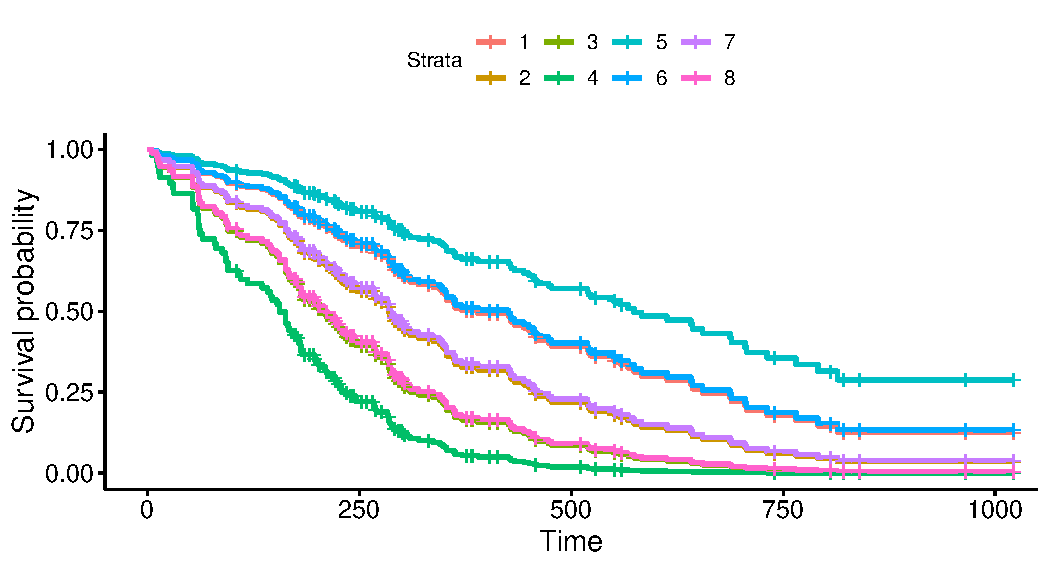
\includegraphics{figure/unnamed-chunk-155-1.pdf}
\caption{plot of chunk unnamed-chunk-155}
\end{figure}

\end{frame}

\begin{frame}[fragile]{Discussion of survival curves}
\protect\hypertarget{discussion-of-survival-curves}{}

\begin{itemize}
\item
  Best survival is teal-blue curve, stratum 5, females with
  (\texttt{ph.ecog}) score 0.
\item
  Next best: blue, stratum 6, females with score 1, and red, stratum 1,
  males score 0.
\item
  Worst: green, stratum 4, males score 3.
\item
  For any given \texttt{ph.ecog} score, females have better predicted
  survival than males.
\item
  For both genders, a lower score associated with better survival.
\end{itemize}

\end{frame}

\begin{frame}[fragile]{The coefficients in model 3}
\protect\hypertarget{the-coefficients-in-model-3}{}

\begin{Shaded}
\begin{Highlighting}[]
\KeywordTok{tidy}\NormalTok{(lung}\FloatTok{.3}\NormalTok{) }\OperatorTok\StringTok{ }\KeywordTok{select}\NormalTok{(term, estimate, p.value)}
\end{Highlighting}
\end{Shaded}

\begin{verbatim}
## # A tibble: 2 x 3
##   term    estimate  p.value
##   <chr>      <dbl>    <dbl>
## 1 sex       -0.510 0.00958 
## 2 ph.ecog    0.483 0.000266
\end{verbatim}

\begin{itemize}
\item
  \texttt{sex} coeff negative, so being higher \texttt{sex} value
  (female) goes with \emph{less} hazard of dying.
\item
  \texttt{ph.ecog} coeff positive, so higher \texttt{ph.ecog} score goes
  with \emph{more} hazard of dying
\item
  Two coeffs about same size, so being male rather than female
  corresponds to 1-point increase in \texttt{ph.ecog} score. Note how
  survival curves come in 3 pairs plus 2 odd.
\end{itemize}

\end{frame}

\begin{frame}[fragile]{Martingale residuals for this model}
\protect\hypertarget{martingale-residuals-for-this-model}{}

No problems here:

\begin{Shaded}
\begin{Highlighting}[]
\KeywordTok{ggcoxdiagnostics}\NormalTok{(lung}\FloatTok{.3}\NormalTok{) }\OperatorTok{+}\StringTok{ }\KeywordTok{geom_smooth}\NormalTok{(}\DataTypeTok{se =}\NormalTok{ F)}
\end{Highlighting}
\end{Shaded}

\begin{verbatim}
## `geom_smooth()` using method = 'loess' and formula 'y ~ x'
\end{verbatim}

\begin{figure}
\centering
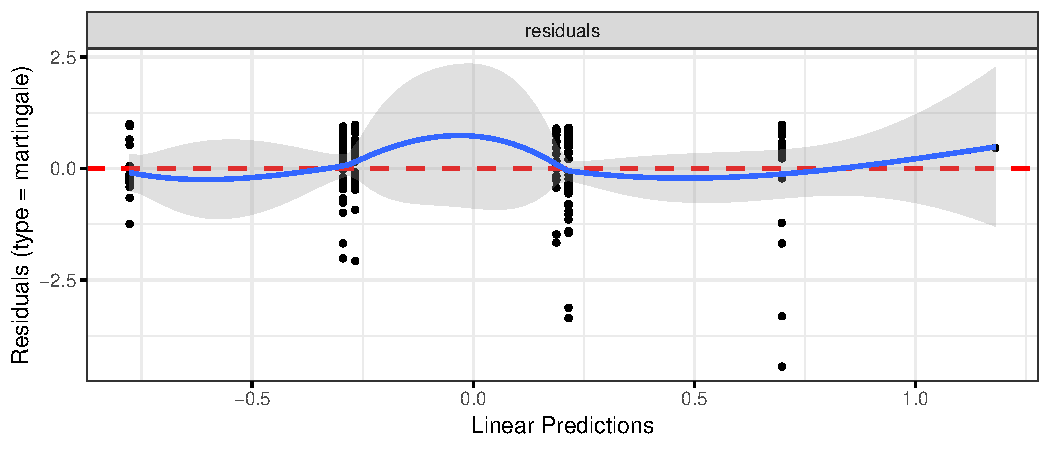
\includegraphics{figure/unnamed-chunk-157-1.pdf}
\caption{plot of chunk unnamed-chunk-157}
\end{figure}

\end{frame}

\begin{frame}[fragile]{When the Cox model fails}
\protect\hypertarget{when-the-cox-model-fails}{}

\begin{itemize}
\tightlist
\item
  Invent some data where survival is best at middling age, and worse at
  high \emph{and} low age:
\end{itemize}

\begin{Shaded}
\begin{Highlighting}[]
\NormalTok{age <-}\StringTok{ }\KeywordTok{seq}\NormalTok{(}\DecValTok{20}\NormalTok{, }\DecValTok{60}\NormalTok{, }\DecValTok{5}\NormalTok{)}
\NormalTok{survtime <-}\StringTok{ }\KeywordTok{c}\NormalTok{(}\DecValTok{10}\NormalTok{, }\DecValTok{12}\NormalTok{, }\DecValTok{11}\NormalTok{, }\DecValTok{21}\NormalTok{, }\DecValTok{15}\NormalTok{, }\DecValTok{20}\NormalTok{, }\DecValTok{8}\NormalTok{, }\DecValTok{9}\NormalTok{, }\DecValTok{11}\NormalTok{)}
\NormalTok{stat <-}\StringTok{ }\KeywordTok{c}\NormalTok{(}\DecValTok{1}\NormalTok{, }\DecValTok{1}\NormalTok{, }\DecValTok{1}\NormalTok{, }\DecValTok{1}\NormalTok{, }\DecValTok{0}\NormalTok{, }\DecValTok{1}\NormalTok{, }\DecValTok{1}\NormalTok{, }\DecValTok{1}\NormalTok{, }\DecValTok{1}\NormalTok{)}
\NormalTok{d <-}\StringTok{ }\KeywordTok{tibble}\NormalTok{(age, survtime, stat)}
\NormalTok{y <-}\StringTok{ }\KeywordTok{with}\NormalTok{(d, }\KeywordTok{Surv}\NormalTok{(survtime, stat))}
\end{Highlighting}
\end{Shaded}

\begin{itemize}
\tightlist
\item
  Small survival time 15 in middle was actually censored, so would have
  been longer if observed.
\end{itemize}

\end{frame}

\begin{frame}[fragile]{Fit Cox model}
\protect\hypertarget{fit-cox-model}{}

\footnotesize

\begin{Shaded}
\begin{Highlighting}[]
\NormalTok{y}\FloatTok{.1}\NormalTok{ <-}\StringTok{ }\KeywordTok{coxph}\NormalTok{(y }\OperatorTok{~}\StringTok{ }\NormalTok{age, }\DataTypeTok{data =}\NormalTok{ d)}
\KeywordTok{summary}\NormalTok{(y}\FloatTok{.1}\NormalTok{)}
\end{Highlighting}
\end{Shaded}

\begin{verbatim}
## Call:
## coxph(formula = y ~ age, data = d)
## 
##   n= 9, number of events= 8 
## 
##        coef exp(coef) se(coef)     z Pr(>|z|)
## age 0.01984   1.02003  0.03446 0.576    0.565
## 
##     exp(coef) exp(-coef) lower .95 upper .95
## age      1.02     0.9804    0.9534     1.091
## 
## Concordance= 0.545  (se = 0.105 )
## Likelihood ratio test= 0.33  on 1 df,   p=0.6
## Wald test            = 0.33  on 1 df,   p=0.6
## Score (logrank) test = 0.33  on 1 df,   p=0.6
\end{verbatim}

\normalsize

\end{frame}

\begin{frame}[fragile]{Martingale residuals}
\protect\hypertarget{martingale-residuals}{}

Down-and-up indicates incorrect relationship between age and survival:

\begin{Shaded}
\begin{Highlighting}[]
\KeywordTok{ggcoxdiagnostics}\NormalTok{(y}\FloatTok{.1}\NormalTok{) }\OperatorTok{+}\StringTok{ }\KeywordTok{geom_smooth}\NormalTok{(}\DataTypeTok{se =}\NormalTok{ F)}
\end{Highlighting}
\end{Shaded}

\begin{figure}
\centering
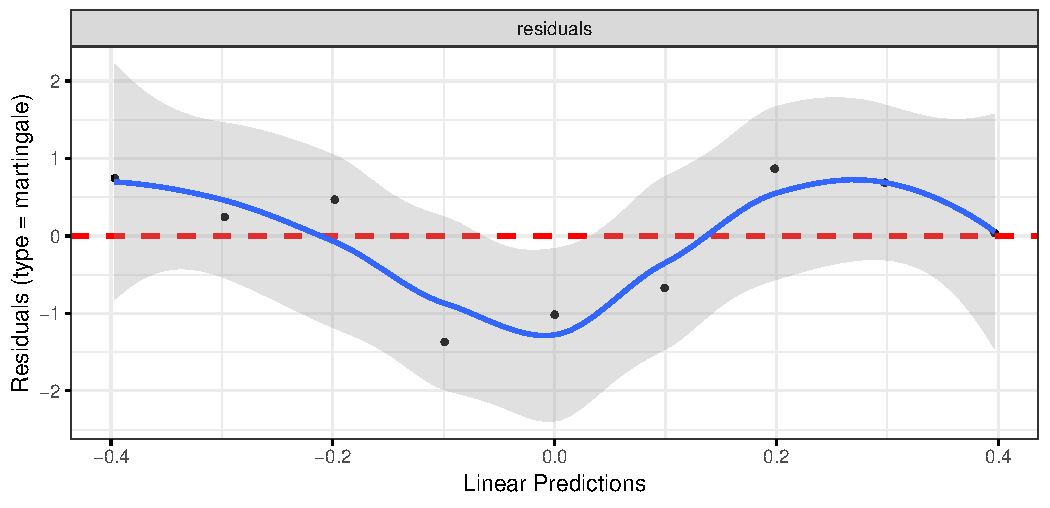
\includegraphics{figure/unnamed-chunk-160-1.pdf}
\caption{plot of chunk unnamed-chunk-160}
\end{figure}

\end{frame}

\begin{frame}[fragile]{Attempt 2}
\protect\hypertarget{attempt-2}{}

Add squared term in age:

\begin{Shaded}
\begin{Highlighting}[]
\NormalTok{y}\FloatTok{.2}\NormalTok{ <-}\StringTok{ }\KeywordTok{coxph}\NormalTok{(y }\OperatorTok{~}\StringTok{ }\NormalTok{age }\OperatorTok{+}\StringTok{ }\KeywordTok{I}\NormalTok{(age}\OperatorTok{^}\DecValTok{2}\NormalTok{), }\DataTypeTok{data =}\NormalTok{ d)}
\KeywordTok{tidy}\NormalTok{(y}\FloatTok{.2}\NormalTok{) }\OperatorTok\StringTok{ }\KeywordTok{select}\NormalTok{(term, estimate, p.value)}
\end{Highlighting}
\end{Shaded}

\begin{verbatim}
## # A tibble: 2 x 3
##   term     estimate p.value
##   <chr>       <dbl>   <dbl>
## 1 age      -0.380    0.116 
## 2 I(age^2)  0.00483  0.0977
\end{verbatim}

\begin{itemize}
\tightlist
\item
  (Marginally) helpful.
\end{itemize}

\end{frame}

\begin{frame}[fragile]{Martingale residuals this time}
\protect\hypertarget{martingale-residuals-this-time}{}

Not great, but less problematic than before:

\begin{Shaded}
\begin{Highlighting}[]
\KeywordTok{ggcoxdiagnostics}\NormalTok{(y}\FloatTok{.2}\NormalTok{) }\OperatorTok{+}\StringTok{ }\KeywordTok{geom_smooth}\NormalTok{(}\DataTypeTok{se =}\NormalTok{ F)}
\end{Highlighting}
\end{Shaded}

\begin{figure}
\centering
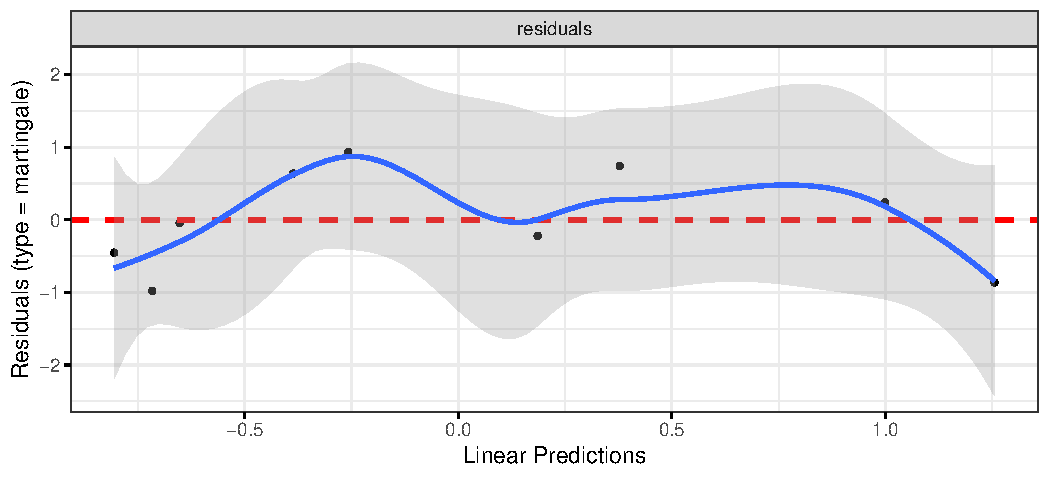
\includegraphics{figure/unnamed-chunk-162-1.pdf}
\caption{plot of chunk unnamed-chunk-162}
\end{figure}

\end{frame}

\hypertarget{analysis-of-variance}{%
\section{Analysis of variance}\label{analysis-of-variance}}

\begin{frame}{Analysis of variance}
\protect\hypertarget{analysis-of-variance-1}{}

\begin{itemize}
\item
  Analysis of variance used with:

  \begin{itemize}
  \item
    counted/measured response
  \item
    categorical explanatory variable(s)
  \item
    that is, data divided into groups, and see if response significantly
    different among groups
  \item
    or, see whether knowing group membership helps to predict response.
  \end{itemize}
\item
  Typically two stages:

  \begin{itemize}
  \item
    \(F\)-test to detect \emph{any} differences among/due to groups
  \item
    if \(F\)-test significant, do \emph{multiple comparisons} to see
    which groups significantly different from which.
  \end{itemize}
\item
  Need special multiple comparisons method because just doing (say)
  two-sample \(t\)-tests on each pair of groups gives too big a chance
  of finding ``significant'' differences by accident.
\end{itemize}

\end{frame}

\begin{frame}[fragile]{Packages}
\protect\hypertarget{packages-2}{}

These:

\begin{Shaded}
\begin{Highlighting}[]
\KeywordTok{library}\NormalTok{(tidyverse)}
\KeywordTok{library}\NormalTok{(broom)}
\KeywordTok{library}\NormalTok{(car) }\CommentTok{# for Levene's text}
\end{Highlighting}
\end{Shaded}

\end{frame}

\begin{frame}{Example: Pain threshold and hair colour}
\protect\hypertarget{example-pain-threshold-and-hair-colour}{}

\begin{itemize}
\item
  Do people with different hair colour have different abilities to deal
  with pain?
\item
  Men and women of various ages divided into 4 groups by hair colour:
  light and dark blond, light and dark brown.
\item
  Each subject given a pain sensitivity test resulting in pain threshold
  score: higher score is higher pain tolerance.
\item
  19 subjects altogether.
\end{itemize}

\end{frame}

\begin{frame}[fragile]{The data}
\protect\hypertarget{the-data-6}{}

In \texttt{hairpain.txt}:

\begin{multicols}{2}

\begin{verbatim}
hair pain
lightblond 62
lightblond 60
lightblond 71
lightblond 55
lightblond 48
darkblond 63
darkblond 57
darkblond 52
darkblond 41
darkblond 43
lightbrown 42
lightbrown 50
lightbrown 41
lightbrown 37
darkbrown 32
darkbrown 39
darkbrown 51
darkbrown 30
darkbrown 35
\end{verbatim}

\end{multicols}

\end{frame}

\begin{frame}[fragile]{Summarizing the groups}
\protect\hypertarget{summarizing-the-groups}{}

\footnotesize

\begin{Shaded}
\begin{Highlighting}[]
\NormalTok{my_url <-}\StringTok{ "http://www.utsc.utoronto.ca/~butler/d29/hairpain.txt"}
\NormalTok{hairpain <-}\StringTok{ }\KeywordTok{read_delim}\NormalTok{(my_url, }\StringTok{" "}\NormalTok{)}
\NormalTok{hairpain }\OperatorTok
\StringTok{  }\KeywordTok{group_by}\NormalTok{(hair) }\OperatorTok
\StringTok{  }\KeywordTok{summarize}\NormalTok{(}
    \DataTypeTok{n =} \KeywordTok{n}\NormalTok{(),}
    \DataTypeTok{xbar =} \KeywordTok{mean}\NormalTok{(pain),}
    \DataTypeTok{s =} \KeywordTok{sd}\NormalTok{(pain)}
\NormalTok{  )}
\end{Highlighting}
\end{Shaded}

\begin{verbatim}
## # A tibble: 4 x 4
##   hair           n  xbar     s
##   <chr>      <int> <dbl> <dbl>
## 1 darkblond      5  51.2  9.28
## 2 darkbrown      5  37.4  8.32
## 3 lightblond     5  59.2  8.53
## 4 lightbrown     4  42.5  5.45
\end{verbatim}

\normalsize

Brown-haired people seem to have lower pain tolerance.

\end{frame}

\begin{frame}[fragile]{Boxplot}
\protect\hypertarget{boxplot}{}

\begin{Shaded}
\begin{Highlighting}[]
\KeywordTok{ggplot}\NormalTok{(hairpain, }\KeywordTok{aes}\NormalTok{(}\DataTypeTok{x =}\NormalTok{ hair, }\DataTypeTok{y =}\NormalTok{ pain)) }\OperatorTok{+}\StringTok{ }\KeywordTok{geom_boxplot}\NormalTok{()}
\end{Highlighting}
\end{Shaded}

\begin{figure}
\centering
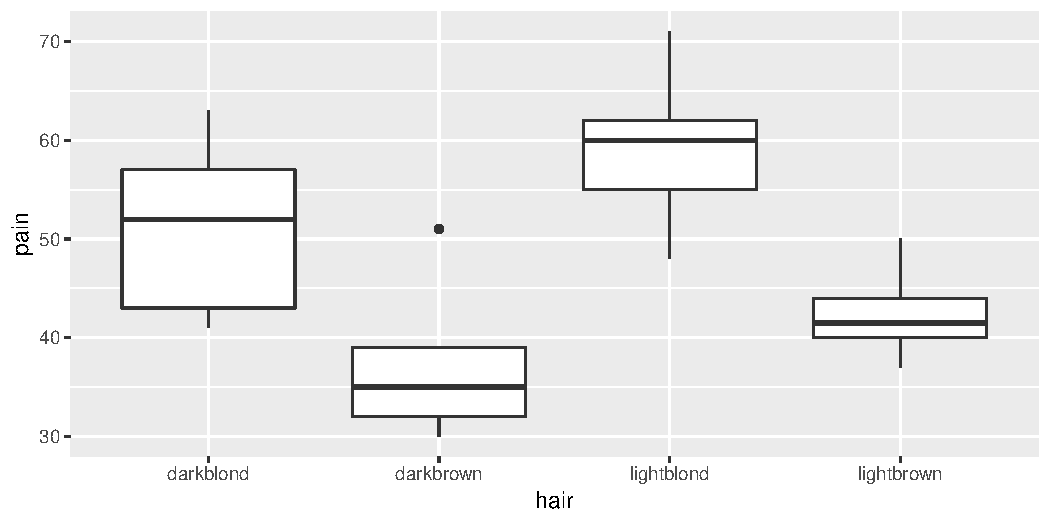
\includegraphics{figure/tartuffo-1.pdf}
\caption{plot of chunk tartuffo}
\end{figure}

\end{frame}

\begin{frame}[fragile]{Assumptions}
\protect\hypertarget{assumptions}{}

\begin{itemize}
\item
  Data should be:

  \begin{itemize}
  \item
    normally distributed within each group
  \item
    same spread for each group
  \end{itemize}
\item
  \texttt{darkbrown} group has upper outlier (suggests not normal)
\item
  \texttt{darkblond} group has smaller IQR than other groups.
\item
  But, groups \emph{small}.
\item
  Shrug shoulders and continue for moment.
\end{itemize}

\end{frame}

\begin{frame}[fragile]{Testing equality of SDs}
\protect\hypertarget{testing-equality-of-sds}{}

\begin{itemize}
\tightlist
\item
  via \textbf{Levene's test} in package \texttt{car}:
\end{itemize}

\small

\begin{Shaded}
\begin{Highlighting}[]
\KeywordTok{leveneTest}\NormalTok{(pain }\OperatorTok{~}\StringTok{ }\NormalTok{hair, }\DataTypeTok{data =}\NormalTok{ hairpain)}
\end{Highlighting}
\end{Shaded}

\begin{verbatim}
## Warning in leveneTest.default(y = y, group = group, ...): group coerced to factor.
\end{verbatim}

\begin{verbatim}
## Levene's Test for Homogeneity of Variance (center = median)
##       Df F value Pr(>F)
## group  3  0.3927   0.76
##       15
\end{verbatim}

\normalsize

\begin{itemize}
\item
  No evidence (at all) of difference among group SDs.
\item
  Possibly because groups \emph{small}.
\end{itemize}

\end{frame}

\begin{frame}[fragile]{Analysis of variance}
\protect\hypertarget{analysis-of-variance-2}{}

\small

\begin{Shaded}
\begin{Highlighting}[]
\NormalTok{hairpain}\FloatTok{.1}\NormalTok{ <-}\StringTok{ }\KeywordTok{aov}\NormalTok{(pain }\OperatorTok{~}\StringTok{ }\NormalTok{hair, }\DataTypeTok{data =}\NormalTok{ hairpain)}
\KeywordTok{summary}\NormalTok{(hairpain}\FloatTok{.1}\NormalTok{)}
\end{Highlighting}
\end{Shaded}

\begin{verbatim}
##             Df Sum Sq Mean Sq F value  Pr(>F)   
## hair         3   1361   453.6   6.791 0.00411 **
## Residuals   15   1002    66.8                   
## ---
## Signif. codes:  0 '***' 0.001 '**' 0.01 '*' 0.05 '.' 0.1 ' ' 1
\end{verbatim}

\normalsize

\begin{itemize}
\item
  P-value small: the mean pain tolerances for the four groups are
  \emph{not} all the same.
\item
  Which groups differ from which, and how?
\end{itemize}

\end{frame}

\begin{frame}{Multiple comparisons}
\protect\hypertarget{multiple-comparisons}{}

\begin{itemize}
\item
  Which groups differ from which? Multiple comparisons method. Lots.
\item
  Problem: by comparing all the groups with each other, doing many
  tests, have large chance to (possibly incorrectly) reject \(H_0:\)
  groups have equal means.
\item
  4 groups: 6 comparisons (1 vs 2, 1 vs 3, \ldots, 3 vs 4). 5 groups: 10
  comparisons. Thus 6 (or 10) chances to make mistake.
\item
  Get ``familywise error rate'' of 0.05 (whatever), no matter how many
  comparisons you're doing.
\item
  My favourite: Tukey, or ``honestly significant differences'': how far
  apart might largest, smallest group means be (if actually no
  differences). Group means more different: significantly different.
\end{itemize}

\end{frame}

\begin{frame}[fragile]{Tukey}
\protect\hypertarget{tukey}{}

\begin{itemize}
\tightlist
\item
  \texttt{TukeyHSD:}
\end{itemize}

\footnotesize

\begin{Shaded}
\begin{Highlighting}[]
\KeywordTok{TukeyHSD}\NormalTok{(hairpain}\FloatTok{.1}\NormalTok{)}
\end{Highlighting}
\end{Shaded}

\begin{verbatim}
##   Tukey multiple comparisons of means
##     95% family-wise confidence level
## 
## Fit: aov(formula = pain ~ hair, data = hairpain)
## 
## $hair
##                        diff        lwr        upr     p adj
## darkbrown-darkblond   -13.8 -28.696741  1.0967407 0.0740679
## lightblond-darkblond    8.0  -6.896741 22.8967407 0.4355768
## lightbrown-darkblond   -8.7 -24.500380  7.1003795 0.4147283
## lightblond-darkbrown   21.8   6.903259 36.6967407 0.0037079
## lightbrown-darkbrown    5.1 -10.700380 20.9003795 0.7893211
## lightbrown-lightblond -16.7 -32.500380 -0.8996205 0.0366467
\end{verbatim}

\normalsize

\end{frame}

\begin{frame}[fragile]{The old-fashioned way}
\protect\hypertarget{the-old-fashioned-way}{}

\begin{itemize}
\item
  List group means in order
\item
  Draw lines connecting groups that are \emph{not} significantly
  different:
\end{itemize}

\begin{verbatim}
darkbrown lightbrown  darkblond lightblond
37.4      42.5       51.2       59.2
-------------------------
                     ---------------
\end{verbatim}

\begin{itemize}
\item
  \texttt{lightblond} significantly higher than everything except
  \texttt{darkblond} (at \(\alpha=0.05\)).
\item
  \texttt{darkblond} in middle ground: not significantly less than
  \texttt{lightblond}, not significantly greater than \texttt{darkbrown}
  and \texttt{lightbrown}.
\item
  More data might resolve this.
\item
  Looks as if blond-haired people do have higher pain tolerance, but not
  completely clear.
\end{itemize}

\end{frame}

\begin{frame}{Some other multiple-comparison methods}
\protect\hypertarget{some-other-multiple-comparison-methods}{}

\begin{itemize}
\item
  Work any time you do \(k\) tests at once (not just ANOVA).

  \begin{itemize}
  \item
    \textbf{Bonferroni}: multiply all P-values by \(k\).
  \item
    \textbf{Holm}: multiply smallest P-value by \(k\), next-smallest by
    \(k-1\), etc.
  \item
    \textbf{False discovery rate}: multiply smallest P-value by \(k/1\),
    2nd-smallest by \(k/2\), \ldots, \(i\)-th smallest by \(k/i\).
  \end{itemize}
\item
  Stop after non-rejection.
\end{itemize}

\end{frame}

\begin{frame}{Example}
\protect\hypertarget{example}{}

\begin{itemize}
\item
  P-values 0.005, 0.015, 0.03, 0.06 (4 tests all done at once) Use
  \(\alpha=0.05\).
\item
  Bonferroni:

  \begin{itemize}
  \item
    Multiply all P-values by 4 (4 tests).
  \item
    Reject only 1st null.
  \end{itemize}
\item
  Holm:

  \begin{itemize}
  \item
    Times smallest P-value by 4: \(0.005*4=0.020<0.05\), reject.
  \item
    Times next smallest by 3: \(0.015*3=0.045<0.05\), reject.
  \item
    Times next smallest by 2: \(0.03*2=0.06>0.05\), do not reject. Stop.
  \end{itemize}
\end{itemize}

\end{frame}

\begin{frame}{\ldots Continued}
\protect\hypertarget{continued}{}

\begin{itemize}
\item
  With P-values 0.005, 0.015, 0.03, 0.06:
\item
  False discovery rate:

  \begin{itemize}
  \item
    Times smallest P-value by 4: \(0.005*4=0.02<0.05\): reject.
  \item
    Times second smallest by \(4/2\): \(0.015*4/2=0.03<0.05\), reject.
  \item
    Times third smallest by \(4/3\): \(0.03*4/3=0.04<0.05\), reject.
  \item
    Times fourth smallest by \(4/4\): \(0.06*4/4=0.06>0.05\), do not
    reject. Stop.
  \end{itemize}
\end{itemize}

\end{frame}

\begin{frame}[fragile]{\texttt{pairwise.t.test}}
\protect\hypertarget{pairwise.t.test}{}

\tiny

\begin{Shaded}
\begin{Highlighting}[]
\KeywordTok{attach}\NormalTok{(hairpain)}
\KeywordTok{pairwise.t.test}\NormalTok{(pain, hair, }\DataTypeTok{p.adj =} \StringTok{"none"}\NormalTok{)}
\end{Highlighting}
\end{Shaded}

\begin{verbatim}
## 
##  Pairwise comparisons using t tests with pooled SD 
## 
## data:  pain and hair 
## 
##            darkblond darkbrown lightblond
## darkbrown  0.01748   -         -         
## lightblond 0.14251   0.00075   -         
## lightbrown 0.13337   0.36695   0.00817   
## 
## P value adjustment method: none
\end{verbatim}

\begin{Shaded}
\begin{Highlighting}[]
\KeywordTok{pairwise.t.test}\NormalTok{(pain, hair, }\DataTypeTok{p.adj =} \StringTok{"holm"}\NormalTok{)}
\end{Highlighting}
\end{Shaded}

\begin{verbatim}
## 
##  Pairwise comparisons using t tests with pooled SD 
## 
## data:  pain and hair 
## 
##            darkblond darkbrown lightblond
## darkbrown  0.0699    -         -         
## lightblond 0.4001    0.0045    -         
## lightbrown 0.4001    0.4001    0.0408    
## 
## P value adjustment method: holm
\end{verbatim}

\normalsize

\end{frame}

\begin{frame}[fragile]{\texttt{pairwise.t.test} part 2}
\protect\hypertarget{pairwise.t.test-part-2}{}

\tiny

\begin{Shaded}
\begin{Highlighting}[]
\KeywordTok{pairwise.t.test}\NormalTok{(pain, hair, }\DataTypeTok{p.adj =} \StringTok{"fdr"}\NormalTok{)}
\end{Highlighting}
\end{Shaded}

\begin{verbatim}
## 
##  Pairwise comparisons using t tests with pooled SD 
## 
## data:  pain and hair 
## 
##            darkblond darkbrown lightblond
## darkbrown  0.0350    -         -         
## lightblond 0.1710    0.0045    -         
## lightbrown 0.1710    0.3670    0.0245    
## 
## P value adjustment method: fdr
\end{verbatim}

\begin{Shaded}
\begin{Highlighting}[]
\KeywordTok{pairwise.t.test}\NormalTok{(pain, hair, }\DataTypeTok{p.adj =} \StringTok{"bon"}\NormalTok{)}
\end{Highlighting}
\end{Shaded}

\begin{verbatim}
## 
##  Pairwise comparisons using t tests with pooled SD 
## 
## data:  pain and hair 
## 
##            darkblond darkbrown lightblond
## darkbrown  0.1049    -         -         
## lightblond 0.8550    0.0045    -         
## lightbrown 0.8002    1.0000    0.0490    
## 
## P value adjustment method: bonferroni
\end{verbatim}

\normalsize

\end{frame}

\begin{frame}{Comments}
\protect\hypertarget{comments-15}{}

\begin{itemize}
\item
  P-values all adjusted upwards from ``none''.
\item
  Required because 6 tests at once.
\item
  Highest P-values for Bonferroni: most ``conservative''.
\item
  Prefer Tukey or FDR or Holm.
\item
  Tukey only applies to ANOVA, not to other cases of multiple testing.
\end{itemize}

\end{frame}

\begin{frame}[fragile]{Rats and vitamin B}
\protect\hypertarget{rats-and-vitamin-b}{}

\begin{itemize}
\item
  What is the effect of dietary vitamin B on the kidney?
\item
  A number of rats were randomized to receive either a B-supplemented
  diet or a regular diet.
\item
  Desired to control for initial size of rats, so classified into size
  classes \texttt{lean} and \texttt{obese}.
\item
  After 20 weeks, rats' kidneys weighed.
\item
  Variables:

  \begin{itemize}
  \item
    Response: \texttt{kidneyweight} (grams).
  \item
    Explanatory: \texttt{diet}, \texttt{ratsize}.
  \end{itemize}
\item
  Read in data:
\end{itemize}

\begin{Shaded}
\begin{Highlighting}[]
\NormalTok{my_url <-}\StringTok{ "http://www.utsc.utoronto.ca/~butler/d29/vitaminb.txt"}
\NormalTok{vitaminb <-}\StringTok{ }\KeywordTok{read_delim}\NormalTok{(my_url, }\StringTok{" "}\NormalTok{)}
\end{Highlighting}
\end{Shaded}

\begin{verbatim}
## Parsed with column specification:
## cols(
##   ratsize = col_character(),
##   diet = col_character(),
##   kidneyweight = col_double()
## )
\end{verbatim}

\end{frame}

\begin{frame}[fragile]{The data}
\protect\hypertarget{the-data-7}{}

\begin{Shaded}
\begin{Highlighting}[]
\NormalTok{vitaminb}
\end{Highlighting}
\end{Shaded}

\begin{verbatim}
## # A tibble: 28 x 3
##    ratsize diet     kidneyweight
##    <chr>   <chr>           <dbl>
##  1 lean    regular          1.62
##  2 lean    regular          1.8 
##  3 lean    regular          1.71
##  4 lean    regular          1.81
##  5 lean    regular          1.47
##  6 lean    regular          1.37
##  7 lean    regular          1.71
##  8 lean    vitaminb         1.51
##  9 lean    vitaminb         1.65
## 10 lean    vitaminb         1.45
## # … with 18 more rows
\end{verbatim}

\end{frame}

\begin{frame}[fragile]{Grouped boxplot}
\protect\hypertarget{grouped-boxplot}{}

\begin{Shaded}
\begin{Highlighting}[]
\KeywordTok{ggplot}\NormalTok{(vitaminb, }\KeywordTok{aes}\NormalTok{(}
  \DataTypeTok{x =}\NormalTok{ ratsize, }\DataTypeTok{y =}\NormalTok{ kidneyweight,}
  \DataTypeTok{fill =}\NormalTok{ diet}
\NormalTok{)) }\OperatorTok{+}\StringTok{ }\KeywordTok{geom_boxplot}\NormalTok{()}
\end{Highlighting}
\end{Shaded}

\begin{figure}
\centering
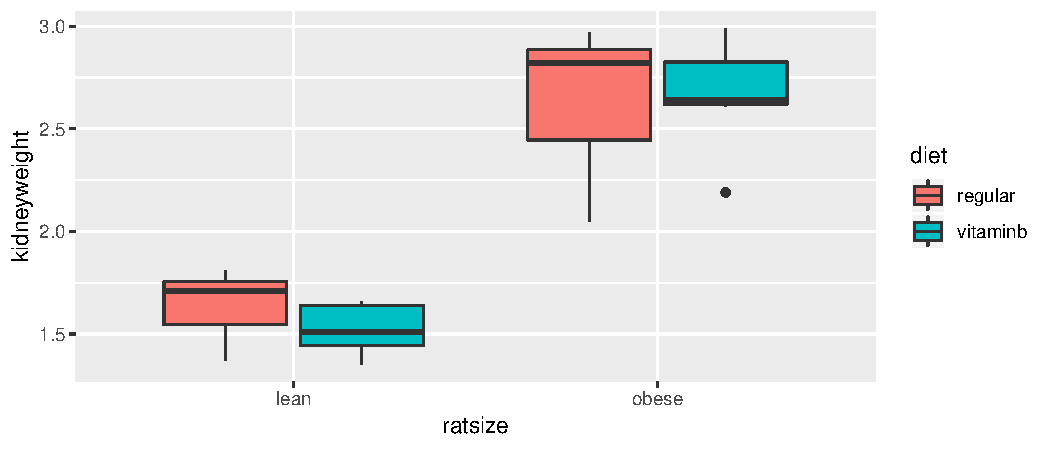
\includegraphics{figure/unnamed-chunk-172-1.pdf}
\caption{plot of chunk unnamed-chunk-172}
\end{figure}

\end{frame}

\begin{frame}[fragile]{What's going on?}
\protect\hypertarget{whats-going-on}{}

\begin{itemize}
\tightlist
\item
  Calculate group means:
\end{itemize}

\footnotesize

\begin{Shaded}
\begin{Highlighting}[]
\NormalTok{summary <-}\StringTok{ }\NormalTok{vitaminb }\OperatorTok
\StringTok{  }\KeywordTok{group_by}\NormalTok{(ratsize, diet) }\OperatorTok
\StringTok{  }\KeywordTok{summarize}\NormalTok{(}\DataTypeTok{mean =} \KeywordTok{mean}\NormalTok{(kidneyweight))}
\NormalTok{summary}
\end{Highlighting}
\end{Shaded}

\begin{verbatim}
## # A tibble: 4 x 3
## # Groups:   ratsize [2]
##   ratsize diet      mean
##   <chr>   <chr>    <dbl>
## 1 lean    regular   1.64
## 2 lean    vitaminb  1.53
## 3 obese   regular   2.64
## 4 obese   vitaminb  2.67
\end{verbatim}

\normalsize

\begin{itemize}
\item
  Rat size: a large and consistent effect.
\item
  Diet: small/no effect (compare same rat size, different diet).
\item
  Effect of rat size \emph{same} for each diet: no interaction.
\end{itemize}

\end{frame}

\begin{frame}[fragile]{ANOVA with interaction}
\protect\hypertarget{anova-with-interaction}{}

\begin{Shaded}
\begin{Highlighting}[]
\NormalTok{vitaminb}\FloatTok{.1}\NormalTok{ <-}\StringTok{ }\KeywordTok{aov}\NormalTok{(kidneyweight }\OperatorTok{~}\StringTok{ }\NormalTok{ratsize }\OperatorTok{*}\StringTok{ }\NormalTok{diet,}
  \DataTypeTok{data =}\NormalTok{ vitaminb}
\NormalTok{)}
\KeywordTok{summary}\NormalTok{(vitaminb}\FloatTok{.1}\NormalTok{)}
\end{Highlighting}
\end{Shaded}

\begin{verbatim}
##              Df Sum Sq Mean Sq F value   Pr(>F)    
## ratsize       1  8.068   8.068 141.179 1.53e-11 ***
## diet          1  0.012   0.012   0.218    0.645    
## ratsize:diet  1  0.036   0.036   0.638    0.432    
## Residuals    24  1.372   0.057                     
## ---
## Signif. codes:  0 '***' 0.001 '**' 0.01 '*' 0.05 '.' 0.1 ' ' 1
\end{verbatim}

\begin{itemize}
\tightlist
\item
  Significance/nonsignificance as we expected.
\item
  Note no significant interaction (can be removed).
\end{itemize}

\end{frame}

\begin{frame}[fragile]{Interaction plot}
\protect\hypertarget{interaction-plot}{}

\begin{itemize}
\tightlist
\item
  Plot mean of response variable against one of the explanatory, using
  other one as groups. Start from \texttt{summary}:
\end{itemize}

\begin{Shaded}
\begin{Highlighting}[]
\NormalTok{g <-}\StringTok{ }\KeywordTok{ggplot}\NormalTok{(summary, }\KeywordTok{aes}\NormalTok{(}
  \DataTypeTok{x =}\NormalTok{ ratsize, }\DataTypeTok{y =}\NormalTok{ mean,}
  \DataTypeTok{colour =}\NormalTok{ diet, }\DataTypeTok{group =}\NormalTok{ diet}
\NormalTok{)) }\OperatorTok{+}
\StringTok{  }\KeywordTok{geom_point}\NormalTok{() }\OperatorTok{+}\StringTok{ }\KeywordTok{geom_line}\NormalTok{()}
\end{Highlighting}
\end{Shaded}

\begin{itemize}
\tightlist
\item
  For this, have to give \emph{both} \texttt{group} and \texttt{colour}.
\end{itemize}

\end{frame}

\begin{frame}[fragile]{The interaction plot}
\protect\hypertarget{the-interaction-plot}{}

\begin{Shaded}
\begin{Highlighting}[]
\NormalTok{g}
\end{Highlighting}
\end{Shaded}

\begin{figure}
\centering
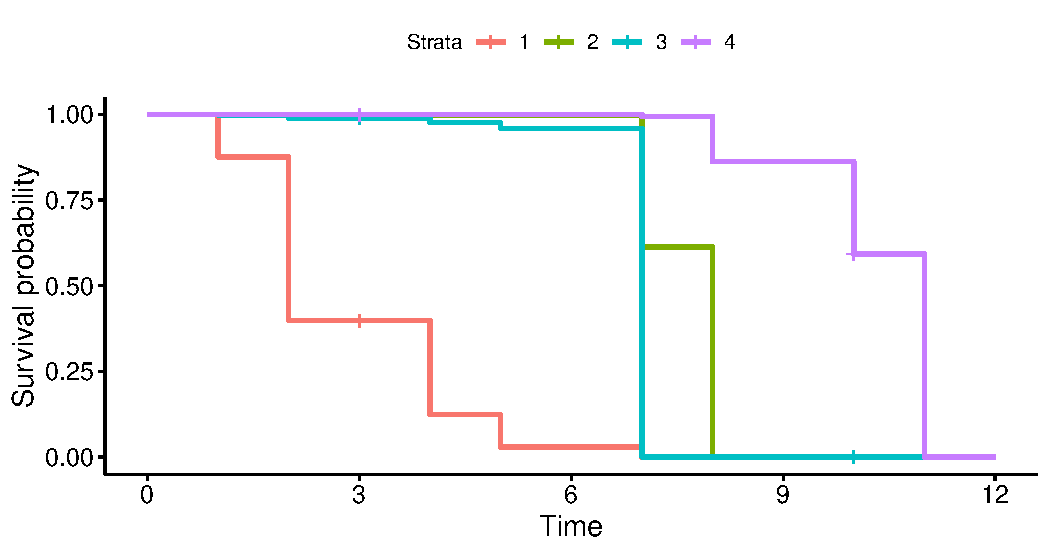
\includegraphics{figure/unnamed-chunk-176-1.pdf}
\caption{plot of chunk unnamed-chunk-176}
\end{figure}

Lines basically parallel, indicating no interaction.

\end{frame}

\begin{frame}[fragile]{Take out interaction}
\protect\hypertarget{take-out-interaction}{}

\small

\begin{Shaded}
\begin{Highlighting}[]
\NormalTok{vitaminb}\FloatTok{.2}\NormalTok{ <-}\StringTok{ }\KeywordTok{update}\NormalTok{(vitaminb}\FloatTok{.1}\NormalTok{, . }\OperatorTok{~}\StringTok{ }\NormalTok{. }\OperatorTok{-}\StringTok{ }\NormalTok{ratsize}\OperatorTok{:}\NormalTok{diet)}
\KeywordTok{summary}\NormalTok{(vitaminb}\FloatTok{.2}\NormalTok{)}
\end{Highlighting}
\end{Shaded}

\begin{verbatim}
##             Df Sum Sq Mean Sq F value   Pr(>F)    
## ratsize      1  8.068   8.068 143.256 7.59e-12 ***
## diet         1  0.012   0.012   0.221    0.643    
## Residuals   25  1.408   0.056                     
## ---
## Signif. codes:  0 '***' 0.001 '**' 0.01 '*' 0.05 '.' 0.1 ' ' 1
\end{verbatim}

\normalsize

\begin{itemize}
\item
  No Tukey for \texttt{diet}: not significant.
\item
  No Tukey for \texttt{ratsize}: only two sizes, and already know that
  obese rats have larger kidneys than lean ones.
\item
  Bottom line: diet has no effect on kidney size once you control for
  size of rat.
\end{itemize}

\end{frame}

\begin{frame}[fragile]{The auto noise data}
\protect\hypertarget{the-auto-noise-data}{}

In 1973, the President of Texaco cited an automobile filter developed by
Associated Octel Company as effective in reducing pollution. However,
questions had been raised about the effects of filter silencing. He
referred to the data included in the report (and below) as evidence that
the silencing properties of the Octel filter were at least equal to
those of standard silencers.

\begin{Shaded}
\begin{Highlighting}[]
\NormalTok{u <-}\StringTok{ "http://www.utsc.utoronto.ca/~butler/d29/autonoise.txt"}
\NormalTok{autonoise <-}\StringTok{ }\KeywordTok{read_table}\NormalTok{(u)}
\end{Highlighting}
\end{Shaded}

\begin{verbatim}
## Parsed with column specification:
## cols(
##   noise = col_double(),
##   size = col_character(),
##   type = col_character(),
##   side = col_character()
## )
\end{verbatim}

\end{frame}

\begin{frame}[fragile]{The data}
\protect\hypertarget{the-data-8}{}

\begin{Shaded}
\begin{Highlighting}[]
\NormalTok{autonoise}
\end{Highlighting}
\end{Shaded}

\begin{verbatim}
## # A tibble: 36 x 4
##    noise size  type  side 
##    <dbl> <chr> <chr> <chr>
##  1   840 M     Std   R    
##  2   770 L     Octel L    
##  3   820 M     Octel R    
##  4   775 L     Octel R    
##  5   825 M     Octel L    
##  6   840 M     Std   R    
##  7   845 M     Std   L    
##  8   825 M     Octel L    
##  9   815 M     Octel L    
## 10   845 M     Std   R    
## # … with 26 more rows
\end{verbatim}

\end{frame}

\begin{frame}[fragile]{Making boxplot}
\protect\hypertarget{making-boxplot}{}

\begin{itemize}
\item
  Make a boxplot, but have combinations of filter type and engine size.
\item
  Use grouped boxplot again, thus:
\end{itemize}

\begin{Shaded}
\begin{Highlighting}[]
\NormalTok{g <-}\StringTok{ }\NormalTok{autonoise }\OperatorTok
\StringTok{  }\KeywordTok{ggplot}\NormalTok{(}\KeywordTok{aes}\NormalTok{(}\DataTypeTok{x =}\NormalTok{ size, }\DataTypeTok{y =}\NormalTok{ noise, }\DataTypeTok{fill =}\NormalTok{ type)) }\OperatorTok{+}
\StringTok{  }\KeywordTok{geom_boxplot}\NormalTok{()}
\end{Highlighting}
\end{Shaded}

\end{frame}

\begin{frame}[fragile]{The boxplot}
\protect\hypertarget{the-boxplot}{}

\begin{itemize}
\item
  See difference in engine noise between Octel and standard is larger
  for medium engine size than for large or small.
\item
  Some evidence of differences in spreads (ignore for now):
\end{itemize}

\begin{Shaded}
\begin{Highlighting}[]
\NormalTok{g}
\end{Highlighting}
\end{Shaded}

\begin{figure}
\centering
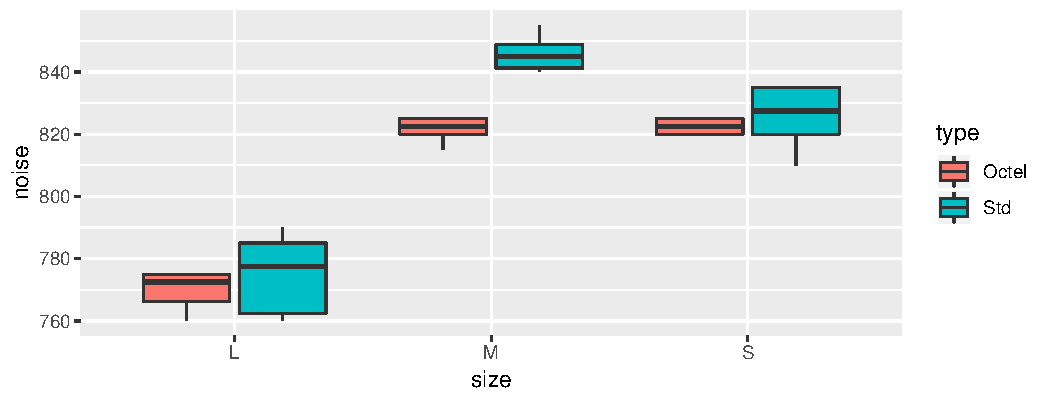
\includegraphics{figure/unnamed-chunk-181-1.pdf}
\caption{plot of chunk unnamed-chunk-181}
\end{figure}

\end{frame}

\begin{frame}[fragile]{ANOVA}
\protect\hypertarget{anova}{}

\small

\begin{Shaded}
\begin{Highlighting}[]
\NormalTok{autonoise}\FloatTok{.1}\NormalTok{ <-}\StringTok{ }\KeywordTok{aov}\NormalTok{(noise }\OperatorTok{~}\StringTok{ }\NormalTok{size }\OperatorTok{*}\StringTok{ }\NormalTok{type, }\DataTypeTok{data =}\NormalTok{ autonoise)}
\KeywordTok{summary}\NormalTok{(autonoise}\FloatTok{.1}\NormalTok{)}
\end{Highlighting}
\end{Shaded}

\begin{verbatim}
##             Df Sum Sq Mean Sq F value   Pr(>F)    
## size         2  26051   13026 199.119  < 2e-16 ***
## type         1   1056    1056  16.146 0.000363 ***
## size:type    2    804     402   6.146 0.005792 ** 
## Residuals   30   1962      65                     
## ---
## Signif. codes:  0 '***' 0.001 '**' 0.01 '*' 0.05 '.' 0.1 ' ' 1
\end{verbatim}

\normalsize

\begin{itemize}
\item
  The interaction is significant, as we suspected from the boxplots.
\item
  The within-group spreads don't look very equal, but only based on 6
  obs each.
\end{itemize}

\end{frame}

\begin{frame}[fragile]{Tukey: ouch!}
\protect\hypertarget{tukey-ouch}{}

\scriptsize

\begin{Shaded}
\begin{Highlighting}[]
\NormalTok{autonoise}\FloatTok{.2}\NormalTok{ <-}\StringTok{ }\KeywordTok{TukeyHSD}\NormalTok{(autonoise}\FloatTok{.1}\NormalTok{)}
\NormalTok{autonoise}\FloatTok{.2}\OperatorTok{$}\StringTok{`}\DataTypeTok{size:type}\StringTok{`}
\end{Highlighting}
\end{Shaded}

\begin{verbatim}
##                        diff        lwr        upr        p adj
## M:Octel-L:Octel  51.6666667  37.463511  65.869823 6.033496e-11
## S:Octel-L:Octel  52.5000000  38.296844  66.703156 4.089762e-11
## L:Std-L:Octel     5.0000000  -9.203156  19.203156 8.890358e-01
## M:Std-L:Octel    75.8333333  61.630177  90.036489 4.962697e-14
## S:Std-L:Octel    55.8333333  41.630177  70.036489 9.002910e-12
## S:Octel-M:Octel   0.8333333 -13.369823  15.036489 9.999720e-01
## L:Std-M:Octel   -46.6666667 -60.869823 -32.463511 6.766649e-10
## M:Std-M:Octel    24.1666667   9.963511  38.369823 1.908995e-04
## S:Std-M:Octel     4.1666667 -10.036489  18.369823 9.454142e-01
## L:Std-S:Octel   -47.5000000 -61.703156 -33.296844 4.477636e-10
## M:Std-S:Octel    23.3333333   9.130177  37.536489 3.129974e-04
## S:Std-S:Octel     3.3333333 -10.869823  17.536489 9.787622e-01
## M:Std-L:Std      70.8333333  56.630177  85.036489 6.583623e-14
## S:Std-L:Std      50.8333333  36.630177  65.036489 8.937329e-11
## S:Std-M:Std     -20.0000000 -34.203156  -5.796844 2.203265e-03
\end{verbatim}

\normalsize

\end{frame}

\begin{frame}[fragile]{Interaction plot}
\protect\hypertarget{interaction-plot-1}{}

\begin{itemize}
\item
  This time, don't have summary of mean noise for each size-type
  combination.
\item
  One way is to compute summaries (means) first, and feed into
  \texttt{ggplot} as in vitamin B example.
\item
  Or, have \texttt{ggplot} compute them for us, thus:
\end{itemize}

\begin{Shaded}
\begin{Highlighting}[]
\NormalTok{g <-}\StringTok{ }\KeywordTok{ggplot}\NormalTok{(autonoise, }\KeywordTok{aes}\NormalTok{(}
  \DataTypeTok{x =}\NormalTok{ size, }\DataTypeTok{y =}\NormalTok{ noise,}
  \DataTypeTok{colour =}\NormalTok{ type, }\DataTypeTok{group =}\NormalTok{ type}
\NormalTok{)) }\OperatorTok{+}
\StringTok{  }\KeywordTok{stat_summary}\NormalTok{(}\DataTypeTok{fun.y =}\NormalTok{ mean, }\DataTypeTok{geom =} \StringTok{"point"}\NormalTok{) }\OperatorTok{+}
\StringTok{  }\KeywordTok{stat_summary}\NormalTok{(}\DataTypeTok{fun.y =}\NormalTok{ mean, }\DataTypeTok{geom =} \StringTok{"line"}\NormalTok{)}
\end{Highlighting}
\end{Shaded}

\end{frame}

\begin{frame}[fragile]{Interaction plot}
\protect\hypertarget{interaction-plot-2}{}

The lines are definitely \emph{not} parallel, showing that the effect of
\texttt{type} is different for medium-sized engines than for others:

\begin{Shaded}
\begin{Highlighting}[]
\NormalTok{g}
\end{Highlighting}
\end{Shaded}

\begin{figure}
\centering
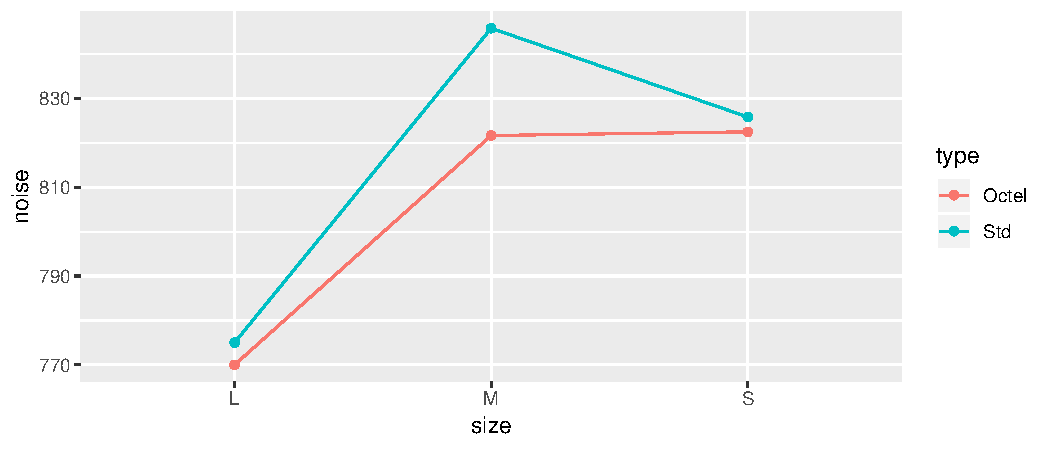
\includegraphics{figure/unnamed-chunk-185-1.pdf}
\caption{plot of chunk unnamed-chunk-185}
\end{figure}

\end{frame}

\begin{frame}[fragile]{If you don't like that\ldots}
\protect\hypertarget{if-you-dont-like-that}{}

\ldots then compute the means first, in a pipeline:

\footnotesize

\begin{Shaded}
\begin{Highlighting}[]
\NormalTok{autonoise }\OperatorTok
\StringTok{  }\KeywordTok{group_by}\NormalTok{(size, type) }\OperatorTok
\StringTok{  }\KeywordTok{summarize}\NormalTok{(}\DataTypeTok{mean_noise =} \KeywordTok{mean}\NormalTok{(noise)) }\OperatorTok
\StringTok{  }\KeywordTok{ggplot}\NormalTok{(}\KeywordTok{aes}\NormalTok{(}
    \DataTypeTok{x =}\NormalTok{ size, }\DataTypeTok{y =}\NormalTok{ mean_noise, }\DataTypeTok{group =}\NormalTok{ type,}
    \DataTypeTok{colour =}\NormalTok{ type}
\NormalTok{  )) }\OperatorTok{+}\StringTok{ }\KeywordTok{geom_point}\NormalTok{() }\OperatorTok{+}\StringTok{ }\KeywordTok{geom_line}\NormalTok{()}
\end{Highlighting}
\end{Shaded}

\begin{figure}
\centering
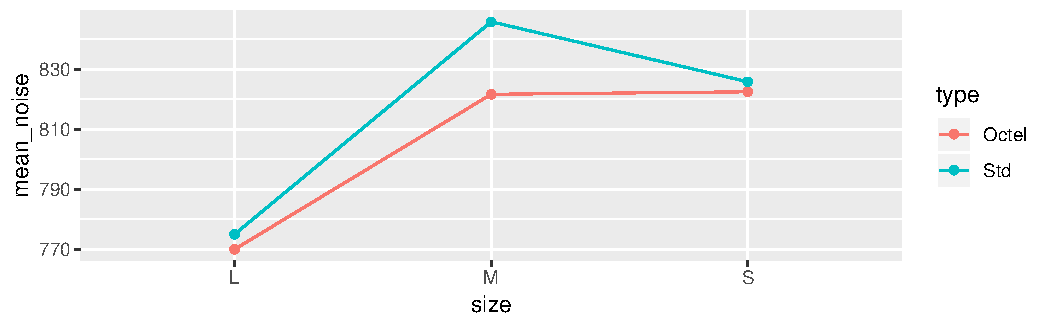
\includegraphics{figure/unnamed-chunk-186-1.pdf}
\caption{plot of chunk unnamed-chunk-186}
\end{figure}

\normalsize

\end{frame}

\begin{frame}{Simple effects for auto noise example}
\protect\hypertarget{simple-effects-for-auto-noise-example}{}

\begin{itemize}
\item
  In auto noise example, weren't interested in all comparisons between
  car size and filter type combinations.
\item
  Wanted to demonstrate (lack of) difference between filter types
  \emph{for each car type}.
\item
  These are called \textbf{simple effects} of one variable (filter type)
  conditional on other variable (car type).
\item
  To do this, pull out just the data for small cars, compare noise for
  the two filter types. Then repeat for medium and large cars. (Three
  one-way ANOVAs.)
\end{itemize}

\end{frame}

\begin{frame}[fragile]{Do it using \texttt{dplyr\ tools}}
\protect\hypertarget{do-it-using-dplyr-tools}{}

\begin{itemize}
\tightlist
\item
  Small cars:
\end{itemize}

\begin{Shaded}
\begin{Highlighting}[]
\NormalTok{autonoise }\OperatorTok
\StringTok{  }\KeywordTok{filter}\NormalTok{(size }\OperatorTok{==}\StringTok{ "S"}\NormalTok{) }\OperatorTok
\StringTok{  }\KeywordTok{aov}\NormalTok{(noise }\OperatorTok{~}\StringTok{ }\NormalTok{type, }\DataTypeTok{data =}\NormalTok{ .) }\OperatorTok
\StringTok{  }\KeywordTok{summary}\NormalTok{()}
\end{Highlighting}
\end{Shaded}

\begin{verbatim}
##             Df Sum Sq Mean Sq F value Pr(>F)
## type         1   33.3   33.33   0.548  0.476
## Residuals   10  608.3   60.83
\end{verbatim}

\begin{itemize}
\item
  No filter difference for small cars.
\item
  For Medium, change \texttt{S} to \texttt{M} and repeat.
\end{itemize}

\end{frame}

\begin{frame}[fragile]{Simple effect of filter type for medium cars}
\protect\hypertarget{simple-effect-of-filter-type-for-medium-cars}{}

\{\small

\begin{Shaded}
\begin{Highlighting}[]
\NormalTok{autonoise }\OperatorTok
\StringTok{  }\KeywordTok{filter}\NormalTok{(size }\OperatorTok{==}\StringTok{ "M"}\NormalTok{) }\OperatorTok
\StringTok{  }\KeywordTok{aov}\NormalTok{(noise }\OperatorTok{~}\StringTok{ }\NormalTok{type, }\DataTypeTok{data =}\NormalTok{ .) }\OperatorTok
\StringTok{  }\KeywordTok{summary}\NormalTok{()}
\end{Highlighting}
\end{Shaded}

\begin{verbatim}
##             Df Sum Sq Mean Sq F value   Pr(>F)    
## type         1 1752.1  1752.1   68.93 8.49e-06 ***
## Residuals   10  254.2    25.4                     
## ---
## Signif. codes:  0 '***' 0.001 '**' 0.01 '*' 0.05 '.' 0.1 ' ' 1
\end{verbatim}

\}

\begin{itemize}
\tightlist
\item
  There \emph{is} an effect of filter type for medium cars. Look at
  means to investigate (over).
\end{itemize}

\end{frame}

\begin{frame}[fragile]{Mean noise for each filter type}
\protect\hypertarget{mean-noise-for-each-filter-type}{}

\ldots for medium engine size:

\begin{Shaded}
\begin{Highlighting}[]
\NormalTok{autonoise }\OperatorTok
\StringTok{  }\KeywordTok{filter}\NormalTok{(size }\OperatorTok{==}\StringTok{ "M"}\NormalTok{) }\OperatorTok
\StringTok{  }\KeywordTok{group_by}\NormalTok{(type) }\OperatorTok
\StringTok{  }\KeywordTok{summarize}\NormalTok{(}\DataTypeTok{m =} \KeywordTok{mean}\NormalTok{(noise))}
\end{Highlighting}
\end{Shaded}

\begin{verbatim}
## # A tibble: 2 x 2
##   type      m
##   <chr> <dbl>
## 1 Octel  822.
## 2 Std    846.
\end{verbatim}

\begin{itemize}
\tightlist
\item
  Octel filters produce \emph{less} noise for medium cars.
\end{itemize}

\end{frame}

\begin{frame}[fragile]{Large cars}
\protect\hypertarget{large-cars}{}

\begin{itemize}
\tightlist
\item
  Large cars:
\end{itemize}

\begin{Shaded}
\begin{Highlighting}[]
\NormalTok{autonoise }\OperatorTok
\StringTok{  }\KeywordTok{filter}\NormalTok{(size }\OperatorTok{==}\StringTok{ "L"}\NormalTok{) }\OperatorTok
\StringTok{  }\KeywordTok{aov}\NormalTok{(noise }\OperatorTok{~}\StringTok{ }\NormalTok{type, }\DataTypeTok{data =}\NormalTok{ .) }\OperatorTok
\StringTok{  }\KeywordTok{summary}\NormalTok{()}
\end{Highlighting}
\end{Shaded}

\begin{verbatim}
##             Df Sum Sq Mean Sq F value Pr(>F)
## type         1     75      75   0.682  0.428
## Residuals   10   1100     110
\end{verbatim}

\begin{itemize}
\tightlist
\item
  No significant difference again.
\end{itemize}

\end{frame}

\begin{frame}[fragile]{Or\ldots }
\protect\hypertarget{or}{}

use \texttt{glance} from \texttt{broom}:

\small

\begin{Shaded}
\begin{Highlighting}[]
\NormalTok{autonoise }\OperatorTok
\StringTok{  }\KeywordTok{filter}\NormalTok{(size }\OperatorTok{==}\StringTok{ "L"}\NormalTok{) }\OperatorTok
\StringTok{  }\KeywordTok{aov}\NormalTok{(noise }\OperatorTok{~}\StringTok{ }\NormalTok{type, }\DataTypeTok{data =}\NormalTok{ .) }\OperatorTok
\StringTok{  }\KeywordTok{glance}\NormalTok{()}
\end{Highlighting}
\end{Shaded}

\begin{verbatim}
## # A tibble: 1 x 11
##   r.squared adj.r.squared sigma statistic p.value    df
##       <dbl>         <dbl> <dbl>     <dbl>   <dbl> <int>
## 1    0.0638       -0.0298  10.5     0.682   0.428     2
## # … with 5 more variables: logLik <dbl>, AIC <dbl>,
## #   BIC <dbl>, deviance <dbl>, df.residual <int>
\end{verbatim}

\normalsize

\begin{itemize}
\tightlist
\item
  P-value same as from \texttt{summary} output.
\end{itemize}

\end{frame}

\begin{frame}[fragile]{All at once, using split/apply/combine}
\protect\hypertarget{all-at-once-using-splitapplycombine}{}

The ``split'' part:

\begin{Shaded}
\begin{Highlighting}[]
\NormalTok{autonoise }\OperatorTok
\StringTok{  }\KeywordTok{group_by}\NormalTok{(size) }\OperatorTok
\StringTok{  }\KeywordTok{nest}\NormalTok{()}
\end{Highlighting}
\end{Shaded}

\begin{verbatim}
## # A tibble: 3 x 2
##   size  data             
##   <chr> <list>           
## 1 M     <tibble [12 × 3]>
## 2 L     <tibble [12 × 3]>
## 3 S     <tibble [12 × 3]>
\end{verbatim}

Now have \emph{three} rows, with the data frame for each size encoded as
\emph{one element} of this data frame.

\end{frame}

\begin{frame}[fragile]{Apply}
\protect\hypertarget{apply}{}

\begin{itemize}
\tightlist
\item
  Write function to do \texttt{aov} on a data frame with columns
  \texttt{noise} and \texttt{type}, returning P-value:
\end{itemize}

\begin{Shaded}
\begin{Highlighting}[]
\NormalTok{aov_pval <-}\StringTok{ }\ControlFlowTok{function}\NormalTok{(x) \{}
\NormalTok{  noise}\FloatTok{.1}\NormalTok{ <-}\StringTok{ }\KeywordTok{aov}\NormalTok{(noise }\OperatorTok{~}\StringTok{ }\NormalTok{type, }\DataTypeTok{data =}\NormalTok{ x)}
\NormalTok{  gg <-}\StringTok{ }\KeywordTok{glance}\NormalTok{(noise}\FloatTok{.1}\NormalTok{)}
\NormalTok{  gg}\OperatorTok{$}\NormalTok{p.value}
\NormalTok{\}}
\end{Highlighting}
\end{Shaded}

\begin{itemize}
\tightlist
\item
  Test it:
\end{itemize}

\begin{Shaded}
\begin{Highlighting}[]
\NormalTok{autonoise }\OperatorTok
\StringTok{  }\KeywordTok{filter}\NormalTok{(size }\OperatorTok{==}\StringTok{ "L"}\NormalTok{) }\OperatorTok
\StringTok{  }\KeywordTok{aov_pval}\NormalTok{()}
\end{Highlighting}
\end{Shaded}

\begin{verbatim}
## [1] 0.428221
\end{verbatim}

\begin{itemize}
\tightlist
\item
  Check.
\end{itemize}

\end{frame}

\begin{frame}[fragile]{Combine}
\protect\hypertarget{combine}{}

\begin{itemize}
\tightlist
\item
  Apply this function to each of the nested data frames (one per engine
  size):
\end{itemize}

\begin{Shaded}
\begin{Highlighting}[]
\NormalTok{autonoise }\OperatorTok
\StringTok{  }\KeywordTok{group_by}\NormalTok{(size) }\OperatorTok
\StringTok{  }\KeywordTok{nest}\NormalTok{() }\OperatorTok
\StringTok{  }\KeywordTok{mutate}\NormalTok{(}\DataTypeTok{p_val =} \KeywordTok{map_dbl}\NormalTok{(data, }\OperatorTok{~}\StringTok{ }\KeywordTok{aov_pval}\NormalTok{(.)))}
\end{Highlighting}
\end{Shaded}

\begin{verbatim}
## # A tibble: 3 x 3
##   size  data                   p_val
##   <chr> <list>                 <dbl>
## 1 M     <tibble [12 × 3]> 0.00000849
## 2 L     <tibble [12 × 3]> 0.428     
## 3 S     <tibble [12 × 3]> 0.476
\end{verbatim}

\begin{itemize}
\tightlist
\item
  \texttt{map\_dbl} because \texttt{aov\_pval} returns a decimal number
  (a \texttt{dbl}). Investigate what happens if you use \texttt{map}
  instead.
\end{itemize}

\end{frame}

\begin{frame}[fragile]{Tidy up}
\protect\hypertarget{tidy-up}{}

\begin{itemize}
\tightlist
\item
  The \texttt{data} column was stepping-stone to getting answer. Don't
  need it any more:
\end{itemize}

\small

\begin{Shaded}
\begin{Highlighting}[]
\NormalTok{simple_effects <-}\StringTok{ }\NormalTok{autonoise }\OperatorTok
\StringTok{  }\KeywordTok{group_by}\NormalTok{(size) }\OperatorTok
\StringTok{  }\KeywordTok{nest}\NormalTok{() }\OperatorTok
\StringTok{  }\KeywordTok{mutate}\NormalTok{(}\DataTypeTok{p_val =} \KeywordTok{map_dbl}\NormalTok{(data, }\OperatorTok{~}\StringTok{ }\KeywordTok{aov_pval}\NormalTok{(.))) }\OperatorTok
\StringTok{  }\KeywordTok{select}\NormalTok{(}\OperatorTok{-}\NormalTok{data)}
\NormalTok{simple_effects}
\end{Highlighting}
\end{Shaded}

\begin{verbatim}
## # A tibble: 3 x 2
##   size       p_val
##   <chr>      <dbl>
## 1 M     0.00000849
## 2 L     0.428     
## 3 S     0.476
\end{verbatim}

\normalsize

\end{frame}

\begin{frame}[fragile]{Simultaneous tests}
\protect\hypertarget{simultaneous-tests}{}

\begin{itemize}
\item
  When testing simple effects, doing several tests at once. (In this
  case, 3.)
\item
  Have to adjust P-values for this. Eg.~Holm:
\end{itemize}

\small

\begin{Shaded}
\begin{Highlighting}[]
\NormalTok{simple_effects }\OperatorTok
\StringTok{  }\KeywordTok{arrange}\NormalTok{(p_val) }\OperatorTok
\StringTok{  }\KeywordTok{mutate}\NormalTok{(}\DataTypeTok{multiplier =} \DecValTok{4} \OperatorTok{-}\StringTok{ }\KeywordTok{row_number}\NormalTok{()) }\OperatorTok
\StringTok{  }\KeywordTok{mutate}\NormalTok{(}\DataTypeTok{p_val_adj =}\NormalTok{ p_val }\OperatorTok{*}\StringTok{ }\NormalTok{multiplier)}
\end{Highlighting}
\end{Shaded}

\begin{verbatim}
## # A tibble: 3 x 4
##   size       p_val multiplier p_val_adj
##   <chr>      <dbl>      <dbl>     <dbl>
## 1 M     0.00000849          3 0.0000255
## 2 L     0.428               2 0.856    
## 3 S     0.476               1 0.476
\end{verbatim}

\normalsize

\begin{footnotesize}

* No change in rejection decisions.

* Octel filters sig.\ better in terms of noise for
medium cars, and not sig.\ different for other sizes.

* Octel filters never significantly worse than standard
ones. 
\end{footnotesize}

\end{frame}

\begin{frame}[fragile]{Confidence intervals}
\protect\hypertarget{confidence-intervals}{}

\begin{itemize}
\item
  Perhaps better way of assessing simple effects: look at
  \emph{confidence intervals} rather than tests.
\item
  Gives us sense of accuracy of estimation, and thus whether
  non-significance might be lack of power: ``absence of evidence is not
  evidence of absence''.
\item
  Works here because \emph{two} filter types, using \texttt{t.test} for
  each engine type.
\item
  Want to show that the Octel filter is equivalent to or better than the
  standard filter, in terms of engine noise.
\end{itemize}

\end{frame}

\begin{frame}[fragile]{Equivalence and noninferiority}
\protect\hypertarget{equivalence-and-noninferiority}{}

\begin{itemize}
\item
  Known as ``equivalence testing'' in medical world. A good read:
  \href{http://www.ncbi.nlm.nih.gov/pmc/articles/PMC3019319/}{link}.
  Basic idea: decide on size of difference \(\delta\) that would be
  considered ``equivalent'', and if CI entirely inside \(\pm \delta\),
  have evidence in favour of equivalence.
\item
  We really want to show that the Octel filters are ``no worse'' than
  the standard one: that is, equivalent \emph{or better} than standard
  filters.
\item
  Such a ``noninferiority test'' done by checking that
  \texttt{upper\ limit} of CI, new minus old, is \emph{less} than
  \(\delta\). (This requires careful thinking about (i) which way around
  the difference is and (ii) whether a higher or lower value is better.)
\end{itemize}

\end{frame}

\begin{frame}[fragile]{CI for small cars}
\protect\hypertarget{ci-for-small-cars}{}

Same idea as for simple effect test:

\begin{Shaded}
\begin{Highlighting}[]
\NormalTok{autonoise }\OperatorTok
\StringTok{  }\KeywordTok{filter}\NormalTok{(size }\OperatorTok{==}\StringTok{ "S"}\NormalTok{) }\OperatorTok
\StringTok{  }\KeywordTok{t.test}\NormalTok{(noise }\OperatorTok{~}\StringTok{ }\NormalTok{type, }\DataTypeTok{data =}\NormalTok{ .) }\OperatorTok
\StringTok{  }\NormalTok{.[[}\StringTok{"conf.int"}\NormalTok{]]}
\end{Highlighting}
\end{Shaded}

\begin{verbatim}
## [1] -14.517462   7.850795
## attr(,"conf.level")
## [1] 0.95
\end{verbatim}

\end{frame}

\begin{frame}[fragile]{CI for medium cars}
\protect\hypertarget{ci-for-medium-cars}{}

\begin{Shaded}
\begin{Highlighting}[]
\NormalTok{autonoise }\OperatorTok
\StringTok{  }\KeywordTok{filter}\NormalTok{(size }\OperatorTok{==}\StringTok{ "M"}\NormalTok{) }\OperatorTok
\StringTok{  }\KeywordTok{t.test}\NormalTok{(noise }\OperatorTok{~}\StringTok{ }\NormalTok{type, }\DataTypeTok{data =}\NormalTok{ .) }\OperatorTok
\StringTok{  }\NormalTok{.[[}\StringTok{"conf.int"}\NormalTok{]]}
\end{Highlighting}
\end{Shaded}

\begin{verbatim}
## [1] -30.75784 -17.57549
## attr(,"conf.level")
## [1] 0.95
\end{verbatim}

\end{frame}

\begin{frame}[fragile]{CI for large cars}
\protect\hypertarget{ci-for-large-cars}{}

\begin{Shaded}
\begin{Highlighting}[]
\NormalTok{autonoise }\OperatorTok
\StringTok{  }\KeywordTok{filter}\NormalTok{(size }\OperatorTok{==}\StringTok{ "L"}\NormalTok{) }\OperatorTok
\StringTok{  }\KeywordTok{t.test}\NormalTok{(noise }\OperatorTok{~}\StringTok{ }\NormalTok{type, }\DataTypeTok{data =}\NormalTok{ .) }\OperatorTok
\StringTok{  }\NormalTok{.[[}\StringTok{"conf.int"}\NormalTok{]]}
\end{Highlighting}
\end{Shaded}

\begin{verbatim}
## [1] -19.270673   9.270673
## attr(,"conf.level")
## [1] 0.95
\end{verbatim}

\end{frame}

\begin{frame}[fragile]{Or, all at once: split/apply/combine}
\protect\hypertarget{or-all-at-once-splitapplycombine}{}

\scriptsize

\begin{Shaded}
\begin{Highlighting}[]
\NormalTok{ci_func <-}\StringTok{ }\ControlFlowTok{function}\NormalTok{(x) \{}
\NormalTok{  tt <-}\StringTok{ }\KeywordTok{t.test}\NormalTok{(noise }\OperatorTok{~}\StringTok{ }\NormalTok{type, }\DataTypeTok{data =}\NormalTok{ x)}
\NormalTok{  tt}\OperatorTok{$}\NormalTok{conf.int}
\NormalTok{\}}
\NormalTok{autonoise }\OperatorTok
\StringTok{  }\KeywordTok{group_by}\NormalTok{(size) }\OperatorTok
\StringTok{  }\KeywordTok{nest}\NormalTok{() }\OperatorTok
\StringTok{  }\KeywordTok{mutate}\NormalTok{(}\DataTypeTok{ci =} \KeywordTok{map}\NormalTok{(data, }\OperatorTok{~}\StringTok{ }\KeywordTok{ci_func}\NormalTok{(.))) }\OperatorTok
\StringTok{  }\KeywordTok{unnest}\NormalTok{(ci) ->}\StringTok{ }\NormalTok{cis}
\end{Highlighting}
\end{Shaded}

\normalsize

\end{frame}

\begin{frame}[fragile]{Results}
\protect\hypertarget{results}{}

\begin{Shaded}
\begin{Highlighting}[]
\NormalTok{cis}
\end{Highlighting}
\end{Shaded}

\begin{verbatim}
## # A tibble: 6 x 2
##   size      ci
##   <chr>  <dbl>
## 1 M     -30.8 
## 2 M     -17.6 
## 3 L     -19.3 
## 4 L       9.27
## 5 S     -14.5 
## 6 S       7.85
\end{verbatim}

\end{frame}

\begin{frame}[fragile]{Procedure}
\protect\hypertarget{procedure}{}

\begin{itemize}
\item
  Function to get CI of difference in noise means for types of filter on
  input data frame
\item
  Group by \texttt{size}, nest (mini-df per size)
\item
  Calculate CI for each thing in \texttt{data} (ie.~each \texttt{size}).
  \texttt{map}: CI is two numbers long
\item
  \texttt{unnest} \texttt{ci} column to see two numbers in each CI.
\end{itemize}

\end{frame}

\begin{frame}[fragile]{CIs and noninferiority test}
\protect\hypertarget{cis-and-noninferiority-test}{}

\begin{itemize}
\item
  Suppose we decide that a 20 dB difference would be considered
  equivalent. (I have no idea whether that is reasonable.)
\item
  Intervals: \vspace{2ex}
\end{itemize}

\small

\begin{Shaded}
\begin{Highlighting}[]
\NormalTok{cis }\OperatorTok
\StringTok{  }\KeywordTok{mutate}\NormalTok{(}\DataTypeTok{hilo =} \KeywordTok{rep}\NormalTok{(}\KeywordTok{c}\NormalTok{(}\StringTok{"lower"}\NormalTok{, }\StringTok{"upper"}\NormalTok{), }\DecValTok{3}\NormalTok{)) }\OperatorTok
\StringTok{  }\KeywordTok{spread}\NormalTok{(hilo, ci)}
\end{Highlighting}
\end{Shaded}

\begin{verbatim}
## # A tibble: 3 x 3
##   size  lower  upper
##   <chr> <dbl>  <dbl>
## 1 L     -19.3   9.27
## 2 M     -30.8 -17.6 
## 3 S     -14.5   7.85
\end{verbatim}

\normalsize

\end{frame}

\begin{frame}{Comments}
\protect\hypertarget{comments-16}{}

\begin{itemize}
\item
  In all cases, upper limit of CI is less than 20 dB. The Octel filters
  are ``noninferior'' to the standard ones.
\item
  Caution: we did 3 procedures at once again. The true confidence level
  is not 95\%. (Won't worry about that here.)
\end{itemize}

\end{frame}

\begin{frame}{Contrasts in ANOVA}
\protect\hypertarget{contrasts-in-anova}{}

\begin{itemize}
\item
  Sometimes, don't want to compare \emph{all} groups, only \emph{some}
  of them.
\item
  Might be able to specify these comparisons ahead of time; other
  comparisons of no interest.
\item
  Wasteful to do ANOVA and Tukey.
\end{itemize}

\end{frame}

\begin{frame}[fragile]{Example: chainsaw kickback}
\protect\hypertarget{example-chainsaw-kickback}{}

\begin{itemize}
\item
  From
  \href{http://www.ohio.edu/plantbio/staff/mccarthy/quantmet/lectures/ANOVA2.pdf}{link}.
\item
  Forest manager concerned about safety of chainsaws issued to field
  crew. 4 models of chainsaws, measure ``kickback'' (degrees of
  deflection) for 5 of each:
\end{itemize}

\begin{verbatim}

 A  B  C  D
-----------
42 28 57 29
17 50 45 29
24 44 48 22
39 32 41 34
43 61 54 30
\end{verbatim}

\begin{itemize}
\tightlist
\item
  So far, standard 1-way ANOVA: what differences are there among models?
\end{itemize}

\end{frame}

\begin{frame}{chainsaw kickback (2)}
\protect\hypertarget{chainsaw-kickback-2}{}

\begin{itemize}
\item
  But: models A and D are designed to be used at home, while models B
  and C are industrial models.
\item
  Suggests these comparisons of interest:
\item
  home vs.~industrial
\item
  the two home models A vs.~D
\item
  the two industrial models B vs.~C.
\item
  Don't need to compare \emph{all} the pairs of models.
\end{itemize}

\end{frame}

\begin{frame}{What is a contrast?}
\protect\hypertarget{what-is-a-contrast}{}

\begin{itemize}
\item
  Contrast is a linear combination of group means.
\item
  Notation: \(\mu_A\) for (population) mean of group \(A\), and so on.
\item
  In example, compare two home models: \(H_0: \mu_A-\mu_D=0\).
\item
  Compare two industrial models: \(H_0: \mu_B-\mu_C=0\).
\item
  Compare average of two home models vs.~average of two industrial
  models: \(H_0: {1\over2}(\mu_A+\mu_D)-{1\over 2}(\mu_B+\mu_C)=0\) or
  \(H_0: 0.5\mu_A-0.5\mu_B-0.5\mu_C+0.5\mu_D=0\).
\item
  Note that coefficients of contrasts add to 0, and right-hand side is
  0.
\end{itemize}

\end{frame}

\begin{frame}[fragile]{Contrasts in R}
\protect\hypertarget{contrasts-in-r}{}

\begin{itemize}
\tightlist
\item
  Comparing two home models A and D (\(\mu_A-\mu_D=0\)):
\end{itemize}

\begin{Shaded}
\begin{Highlighting}[]
\NormalTok{c.home <-}\StringTok{ }\KeywordTok{c}\NormalTok{(}\DecValTok{1}\NormalTok{, }\DecValTok{0}\NormalTok{, }\DecValTok{0}\NormalTok{, }\DecValTok{-1}\NormalTok{)}
\end{Highlighting}
\end{Shaded}

\begin{itemize}
\tightlist
\item
  Comparing two industrial models B and C (\(\mu_B-\mu_C=0\)):
\end{itemize}

\begin{Shaded}
\begin{Highlighting}[]
\NormalTok{c.industrial <-}\StringTok{ }\KeywordTok{c}\NormalTok{(}\DecValTok{0}\NormalTok{, }\DecValTok{1}\NormalTok{, }\DecValTok{-1}\NormalTok{, }\DecValTok{0}\NormalTok{)}
\end{Highlighting}
\end{Shaded}

\begin{itemize}
\tightlist
\item
  Comparing home average vs.~industrial average
  (\(0.5\mu_A-0.5\mu_B-0.5\mu_C+0.5\mu_D=0\)):
\end{itemize}

\begin{Shaded}
\begin{Highlighting}[]
\NormalTok{c.home.ind <-}\StringTok{ }\KeywordTok{c}\NormalTok{(}\FloatTok{0.5}\NormalTok{, }\FloatTok{-0.5}\NormalTok{, }\FloatTok{-0.5}\NormalTok{, }\FloatTok{0.5}\NormalTok{)}
\end{Highlighting}
\end{Shaded}

\end{frame}

\begin{frame}[fragile]{Orthogonal contrasts}
\protect\hypertarget{orthogonal-contrasts}{}

\begin{itemize}
\tightlist
\item
  What happens if we multiply the contrast coefficients one by one?
\end{itemize}

\begin{Shaded}
\begin{Highlighting}[]
\NormalTok{c.home }\OperatorTok{*}\StringTok{ }\NormalTok{c.industrial}
\end{Highlighting}
\end{Shaded}

\begin{verbatim}
## [1] 0 0 0 0
\end{verbatim}

\begin{Shaded}
\begin{Highlighting}[]
\NormalTok{c.home }\OperatorTok{*}\StringTok{ }\NormalTok{c.home.ind}
\end{Highlighting}
\end{Shaded}

\begin{verbatim}
## [1]  0.5  0.0  0.0 -0.5
\end{verbatim}

\begin{Shaded}
\begin{Highlighting}[]
\NormalTok{c.industrial }\OperatorTok{*}\StringTok{ }\NormalTok{c.home.ind}
\end{Highlighting}
\end{Shaded}

\begin{verbatim}
## [1]  0.0 -0.5  0.5  0.0
\end{verbatim}

\begin{itemize}
\tightlist
\item
  in each case, the results \textbf{add up to zero}. Such contrasts are
  called \textbf{orthogonal}.
\end{itemize}

\end{frame}

\begin{frame}[fragile]{Orthogonal contrasts (2)}
\protect\hypertarget{orthogonal-contrasts-2}{}

\begin{itemize}
\tightlist
\item
  Compare these:
\end{itemize}

\normalsize

\begin{Shaded}
\begin{Highlighting}[]
\NormalTok{c1 <-}\StringTok{ }\KeywordTok{c}\NormalTok{(}\DecValTok{1}\NormalTok{, }\DecValTok{-1}\NormalTok{, }\DecValTok{0}\NormalTok{)}
\NormalTok{c2 <-}\StringTok{ }\KeywordTok{c}\NormalTok{(}\DecValTok{0}\NormalTok{, }\DecValTok{1}\NormalTok{, }\DecValTok{-1}\NormalTok{)}
\KeywordTok{sum}\NormalTok{(c1 }\OperatorTok{*}\StringTok{ }\NormalTok{c2)}
\end{Highlighting}
\end{Shaded}

\begin{verbatim}
## [1] -1
\end{verbatim}

\normalsize

Not zero, so \texttt{c1} and \texttt{c2} are \emph{not} orthogonal.

\begin{itemize}
\item
  Orthogonal contrasts are much easier to deal with.
\item
  Can use non-orthogonal contrasts, but more trouble (beyond us).
\end{itemize}

\end{frame}

\begin{frame}[fragile]{Read in data}
\protect\hypertarget{read-in-data-1}{}

\small

\begin{Shaded}
\begin{Highlighting}[]
\NormalTok{url <-}\StringTok{ "http://www.utsc.utoronto.ca/~butler/d29/chainsaw.txt"}
\NormalTok{chain.wide <-}\StringTok{ }\KeywordTok{read_table}\NormalTok{(url)}
\NormalTok{chain.wide}
\end{Highlighting}
\end{Shaded}

\begin{verbatim}
## # A tibble: 5 x 4
##       A     B     C     D
##   <dbl> <dbl> <dbl> <dbl>
## 1    42    28    57    29
## 2    17    50    45    29
## 3    24    44    48    22
## 4    39    32    41    34
## 5    43    61    54    30
\end{verbatim}

\normalsize

\end{frame}

\begin{frame}[fragile]{Tidying}
\protect\hypertarget{tidying}{}

Need all the kickbacks in \emph{one} column:

\begin{Shaded}
\begin{Highlighting}[]
\NormalTok{chain <-}\StringTok{ }\KeywordTok{gather}\NormalTok{(chain.wide, model, kickback, A}\OperatorTok{:}\NormalTok{D,}
  \DataTypeTok{factor_key =}\NormalTok{ T}
\NormalTok{)}
\end{Highlighting}
\end{Shaded}

\end{frame}

\begin{frame}[fragile]{Starting the analysis (2)}
\protect\hypertarget{starting-the-analysis-2}{}

The proper data frame (tiny):

\tiny

\begin{Shaded}
\begin{Highlighting}[]
\NormalTok{chain }
\end{Highlighting}
\end{Shaded}

\begin{verbatim}
## # A tibble: 20 x 2
##    model kickback
##    <fct>    <dbl>
##  1 A           42
##  2 A           17
##  3 A           24
##  4 A           39
##  5 A           43
##  6 B           28
##  7 B           50
##  8 B           44
##  9 B           32
## 10 B           61
## 11 C           57
## 12 C           45
## 13 C           48
## 14 C           41
## 15 C           54
## 16 D           29
## 17 D           29
## 18 D           22
## 19 D           34
## 20 D           30
\end{verbatim}

\normalsize

\end{frame}

\begin{frame}[fragile]{Setting up contrasts}
\protect\hypertarget{setting-up-contrasts}{}

\begin{Shaded}
\begin{Highlighting}[]
\NormalTok{m <-}\StringTok{ }\KeywordTok{cbind}\NormalTok{(c.home, c.industrial, c.home.ind)}
\NormalTok{m}
\end{Highlighting}
\end{Shaded}

\begin{verbatim}
##      c.home c.industrial c.home.ind
## [1,]      1            0        0.5
## [2,]      0            1       -0.5
## [3,]      0           -1       -0.5
## [4,]     -1            0        0.5
\end{verbatim}

\begin{Shaded}
\begin{Highlighting}[]
\KeywordTok{contrasts}\NormalTok{(chain}\OperatorTok{$}\NormalTok{model) <-}\StringTok{ }\NormalTok{m}
\end{Highlighting}
\end{Shaded}

\end{frame}

\begin{frame}[fragile]{ANOVA \emph{as if regression}}
\protect\hypertarget{anova-as-if-regression}{}

\scriptsize

\begin{Shaded}
\begin{Highlighting}[]
\NormalTok{chain}\FloatTok{.1}\NormalTok{ <-}\StringTok{ }\KeywordTok{lm}\NormalTok{(kickback }\OperatorTok{~}\StringTok{ }\NormalTok{model, }\DataTypeTok{data =}\NormalTok{ chain)}
\KeywordTok{summary}\NormalTok{(chain}\FloatTok{.1}\NormalTok{)}
\end{Highlighting}
\end{Shaded}

\begin{verbatim}
## 
## Call:
## lm(formula = kickback ~ model, data = chain)
## 
## Residuals:
##    Min     1Q Median     3Q    Max 
## -16.00  -7.10   0.60   6.25  18.00 
## 
## Coefficients:
##                   Estimate Std. Error t value Pr(>|t|)    
## (Intercept)         38.450      2.179  17.649 6.52e-12 ***
## modelc.home          2.100      3.081   0.682  0.50524    
## modelc.industrial   -3.000      3.081  -0.974  0.34469    
## modelc.home.ind    -15.100      4.357  -3.466  0.00319 ** 
## ---
## Signif. codes:  
## 0 '***' 0.001 '**' 0.01 '*' 0.05 '.' 0.1 ' ' 1
## 
## Residual standard error: 9.743 on 16 degrees of freedom
## Multiple R-squared:  0.4562, Adjusted R-squared:  0.3542 
## F-statistic: 4.474 on 3 and 16 DF,  p-value: 0.01833
\end{verbatim}

\normalsize

\end{frame}

\begin{frame}[fragile]{Conclusions}
\protect\hypertarget{conclusions-2}{}

\begin{Shaded}
\begin{Highlighting}[]
\KeywordTok{tidy}\NormalTok{(chain}\FloatTok{.1}\NormalTok{) }\OperatorTok\StringTok{ }\KeywordTok{select}\NormalTok{(term, p.value)}
\end{Highlighting}
\end{Shaded}

\begin{verbatim}
## # A tibble: 4 x 2
##   term               p.value
##   <chr>                <dbl>
## 1 (Intercept)       6.52e-12
## 2 modelc.home       5.05e- 1
## 3 modelc.industrial 3.45e- 1
## 4 modelc.home.ind   3.19e- 3
\end{verbatim}

\begin{itemize}
\item
  Two home models not sig.~diff.~(P-value 0.51)
\item
  Two industrial models not sig.~diff.~(P-value 0.34)
\item
  Home, industrial models \emph{are} sig.~diff.~(P-value 0.0032).
\end{itemize}

\end{frame}

\begin{frame}[fragile]{Means by model}
\protect\hypertarget{means-by-model}{}

\begin{itemize}
\tightlist
\item
  The means:
\end{itemize}

\footnotesize

\begin{Shaded}
\begin{Highlighting}[]
\NormalTok{chain }\OperatorTok
\StringTok{  }\KeywordTok{group_by}\NormalTok{(model) }\OperatorTok
\StringTok{  }\KeywordTok{summarize}\NormalTok{(}\DataTypeTok{mean.kick =} \KeywordTok{mean}\NormalTok{(kickback)) }\OperatorTok
\StringTok{  }\KeywordTok{arrange}\NormalTok{(}\KeywordTok{desc}\NormalTok{(mean.kick))}
\end{Highlighting}
\end{Shaded}

\begin{verbatim}
## # A tibble: 4 x 2
##   model mean.kick
##   <fct>     <dbl>
## 1 C          49  
## 2 B          43  
## 3 A          33  
## 4 D          28.8
\end{verbatim}

\normalsize

\begin{itemize}
\item
  Home models A \& D have less kickback than industrial ones B \& C.
\item
  Makes sense because industrial users should get training to cope with
  additional kickback.
\end{itemize}

\end{frame}

\hypertarget{analysis-of-covariance}{%
\section{Analysis of covariance}\label{analysis-of-covariance}}

\begin{frame}[fragile]{Analysis of covariance}
\protect\hypertarget{analysis-of-covariance-1}{}

\begin{itemize}
\item
  ANOVA: explanatory variables categorical (divide data into groups)
\item
  traditionally, analysis of covariance has categorical \(x\)'s plus one
  numerical \(x\) (``covariate'') to be adjusted for.
\item
  \texttt{lm} handles this too.
\item
  Simple example: two treatments (drugs) (\texttt{a} and \texttt{b}),
  with before and after scores.
\item
  Does knowing before score and/or treatment help to predict after
  score?
\item
  Is after score different by treatment/before score?
\end{itemize}

\end{frame}

\begin{frame}[fragile]{Data}
\protect\hypertarget{data-1}{}

Treatment, before, after:

\scriptsize

\begin{verbatim}
a 5 20
a 10 23
a 12 30
a 9 25
a 23 34
a 21 40
a 14 27
a 18 38
a 6 24
a 13 31
b 7 19
b 12 26
b 27 33
b 24 35
b 18 30
b 22 31
b 26 34
b 21 28
b 14 23
b 9 22
\end{verbatim}

\normalsize

\end{frame}

\begin{frame}[fragile]{Packages}
\protect\hypertarget{packages-3}{}

\texttt{tidyverse} and \texttt{broom}:

\begin{Shaded}
\begin{Highlighting}[]
\KeywordTok{library}\NormalTok{(tidyverse)}
\KeywordTok{library}\NormalTok{(broom)}
\end{Highlighting}
\end{Shaded}

\end{frame}

\begin{frame}[fragile]{Read in data}
\protect\hypertarget{read-in-data-2}{}

\begin{Shaded}
\begin{Highlighting}[]
\NormalTok{url <-}\StringTok{ "http://www.utsc.utoronto.ca/~butler/d29/ancova.txt"}
\NormalTok{prepost <-}\StringTok{ }\KeywordTok{read_delim}\NormalTok{(url, }\StringTok{" "}\NormalTok{)}
\NormalTok{prepost }\OperatorTok\StringTok{ }\KeywordTok{sample_n}\NormalTok{(}\DecValTok{9}\NormalTok{) }\CommentTok{# randomly chosen rows}
\end{Highlighting}
\end{Shaded}

\begin{verbatim}
## # A tibble: 9 x 3
##   drug  before after
##   <chr>  <dbl> <dbl>
## 1 b         22    31
## 2 b          9    22
## 3 a         18    38
## 4 a         12    30
## 5 b         26    34
## 6 a         14    27
## 7 b         27    33
## 8 a          5    20
## 9 a          6    24
\end{verbatim}

\end{frame}

\begin{frame}[fragile]{Making a plot}
\protect\hypertarget{making-a-plot-1}{}

\begin{Shaded}
\begin{Highlighting}[]
\KeywordTok{ggplot}\NormalTok{(prepost, }\KeywordTok{aes}\NormalTok{(}\DataTypeTok{x =}\NormalTok{ before, }\DataTypeTok{y =}\NormalTok{ after, }\DataTypeTok{colour =}\NormalTok{ drug)) }\OperatorTok{+}
\StringTok{  }\KeywordTok{geom_point}\NormalTok{()}
\end{Highlighting}
\end{Shaded}

\begin{figure}
\centering
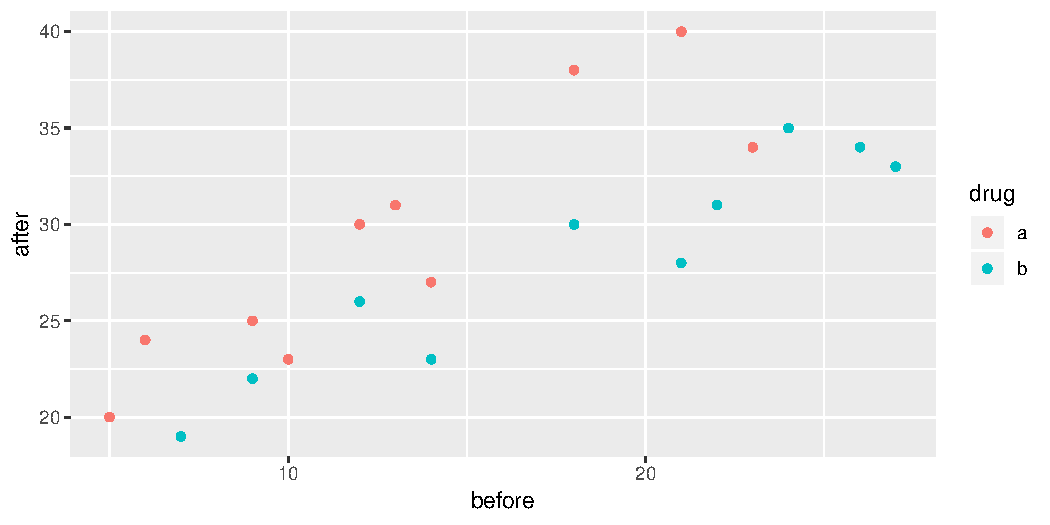
\includegraphics{figure/ancova-plot-1.pdf}
\caption{plot of chunk ancova-plot}
\end{figure}

\end{frame}

\begin{frame}{Comments}
\protect\hypertarget{comments-17}{}

\begin{itemize}
\item
  As before score goes up, after score goes up.
\item
  Red points (drug A) generally above blue points (drug B), for
  comparable before score.
\item
  Suggests before score effect \emph{and} drug effect.
\end{itemize}

\end{frame}

\begin{frame}[fragile]{The means}
\protect\hypertarget{the-means}{}

\begin{Shaded}
\begin{Highlighting}[]
\NormalTok{prepost }\OperatorTok
\StringTok{  }\KeywordTok{group_by}\NormalTok{(drug) }\OperatorTok
\StringTok{  }\KeywordTok{summarize}\NormalTok{(}
    \DataTypeTok{before_mean =} \KeywordTok{mean}\NormalTok{(before),}
    \DataTypeTok{after_mean =} \KeywordTok{mean}\NormalTok{(after)}
\NormalTok{  )}
\end{Highlighting}
\end{Shaded}

\begin{verbatim}
## # A tibble: 2 x 3
##   drug  before_mean after_mean
##   <chr>       <dbl>      <dbl>
## 1 a            13.1       29.2
## 2 b            18         28.1
\end{verbatim}

\begin{itemize}
\item
  Mean ``after'' score slightly higher for treatment A.
\item
  Mean ``before'' score much higher for treatment B.
\item
  Greater \emph{improvement} on treatment A.
\end{itemize}

\end{frame}

\begin{frame}[fragile]{Testing for interaction}
\protect\hypertarget{testing-for-interaction}{}

\begin{Shaded}
\begin{Highlighting}[]
\NormalTok{prepost}\FloatTok{.1}\NormalTok{ <-}\StringTok{ }\KeywordTok{lm}\NormalTok{(after }\OperatorTok{~}\StringTok{ }\NormalTok{before }\OperatorTok{*}\StringTok{ }\NormalTok{drug, }\DataTypeTok{data =}\NormalTok{ prepost)}
\KeywordTok{anova}\NormalTok{(prepost}\FloatTok{.1}\NormalTok{)}
\end{Highlighting}
\end{Shaded}

\begin{verbatim}
## Analysis of Variance Table
## 
## Response: after
##             Df Sum Sq Mean Sq F value    Pr(>F)    
## before       1 430.92  430.92 62.6894  6.34e-07 ***
## drug         1 115.31  115.31 16.7743 0.0008442 ***
## before:drug  1  12.34   12.34  1.7948 0.1990662    
## Residuals   16 109.98    6.87                      
## ---
## Signif. codes:  
## 0 '***' 0.001 '**' 0.01 '*' 0.05 '.' 0.1 ' ' 1
\end{verbatim}

\begin{itemize}
\tightlist
\item
  Interaction not significant. Will remove later.
\end{itemize}

\end{frame}

\begin{frame}[fragile]{Predictions, with interaction included}
\protect\hypertarget{predictions-with-interaction-included}{}

Make combinations of before score and drug:

\begin{Shaded}
\begin{Highlighting}[]
\NormalTok{new <-}\StringTok{ }\KeywordTok{crossing}\NormalTok{(}
  \DataTypeTok{before =} \KeywordTok{c}\NormalTok{(}\DecValTok{5}\NormalTok{, }\DecValTok{15}\NormalTok{, }\DecValTok{25}\NormalTok{),}
  \DataTypeTok{drug =} \KeywordTok{c}\NormalTok{(}\StringTok{"a"}\NormalTok{, }\StringTok{"b"}\NormalTok{)}
\NormalTok{)}
\NormalTok{new}
\end{Highlighting}
\end{Shaded}

\begin{verbatim}
## # A tibble: 6 x 2
##   before drug 
##    <dbl> <chr>
## 1      5 a    
## 2      5 b    
## 3     15 a    
## 4     15 b    
## 5     25 a    
## 6     25 b
\end{verbatim}

\end{frame}

\begin{frame}[fragile]{Do predictions:}
\protect\hypertarget{do-predictions}{}

\begin{Shaded}
\begin{Highlighting}[]
\NormalTok{pred <-}\StringTok{ }\KeywordTok{predict}\NormalTok{(prepost}\FloatTok{.1}\NormalTok{, new)}
\NormalTok{preds <-}\StringTok{ }\KeywordTok{bind_cols}\NormalTok{(new, }\DataTypeTok{pred =}\NormalTok{ pred)}
\NormalTok{preds}
\end{Highlighting}
\end{Shaded}

\begin{verbatim}
## # A tibble: 6 x 3
##   before drug   pred
##    <dbl> <chr> <dbl>
## 1      5 a      21.3
## 2      5 b      18.7
## 3     15 a      31.1
## 4     15 b      25.9
## 5     25 a      40.8
## 6     25 b      33.2
\end{verbatim}

\end{frame}

\begin{frame}[fragile]{Making a plot with lines for each \texttt{drug}}
\protect\hypertarget{making-a-plot-with-lines-for-each-drug}{}

\begin{Shaded}
\begin{Highlighting}[]
\NormalTok{g <-}\StringTok{ }\KeywordTok{ggplot}\NormalTok{(prepost,}
  \KeywordTok{aes}\NormalTok{(}\DataTypeTok{x =}\NormalTok{ before, }\DataTypeTok{y =}\NormalTok{ after, }\DataTypeTok{colour =}\NormalTok{ drug)) }\OperatorTok{+}
\StringTok{  }\KeywordTok{geom_point}\NormalTok{() }\OperatorTok{+}\StringTok{ }\KeywordTok{geom_line}\NormalTok{(}\DataTypeTok{data =}\NormalTok{ preds, }\KeywordTok{aes}\NormalTok{(}\DataTypeTok{y =}\NormalTok{ pred))}
\end{Highlighting}
\end{Shaded}

\begin{itemize}
\item
  Here, final line:

  \begin{itemize}
  \item
    joins points by lines \emph{for different data
    set} (\texttt{preds} rather than \texttt{prepost}),
  \item
    \emph{different \(y\)} (\texttt{pred} rather than \texttt{after}),
  \item
    but same \(x\) (\texttt{x=before} inherited from first
    \texttt{aes}).
  \end{itemize}
\item
  Last line could (more easily) be
\end{itemize}

\begin{Shaded}
\begin{Highlighting}[]
\KeywordTok{geom_smooth}\NormalTok{(}\DataTypeTok{method =} \StringTok{"lm"}\NormalTok{, }\DataTypeTok{se =}\NormalTok{ F)}
\end{Highlighting}
\end{Shaded}

which would work here, but not for later plot.

\end{frame}

\begin{frame}{The plot}
\protect\hypertarget{the-plot-5}{}

\begin{itemize}
\item
  Lines almost parallel, but not quite.
\item
  Non-parallelism (interaction) not significant:
\end{itemize}

\begin{figure}
\centering
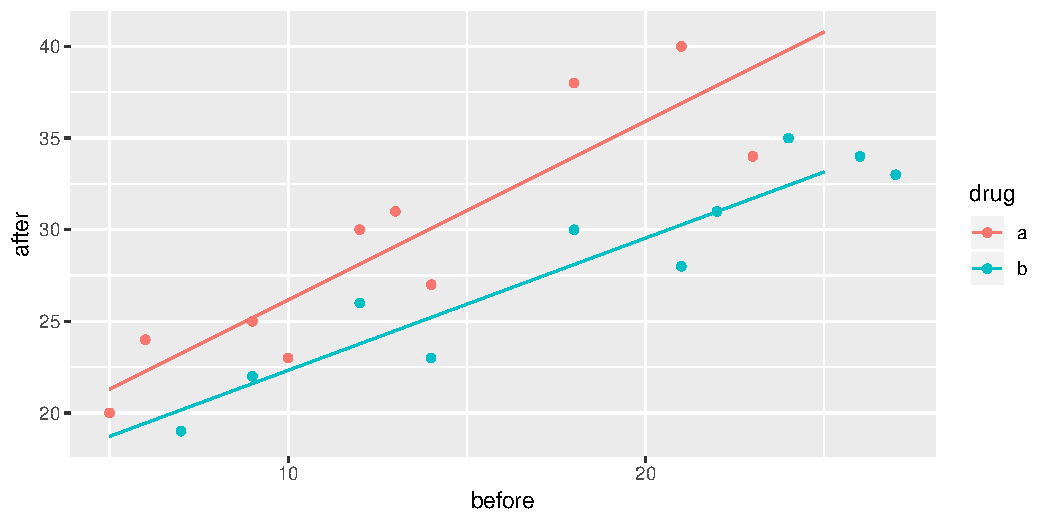
\includegraphics{figure/nachwazzo-1.pdf}
\caption{plot of chunk nachwazzo}
\end{figure}

\end{frame}

\begin{frame}[fragile]{Taking out interaction}
\protect\hypertarget{taking-out-interaction}{}

\small

\begin{Shaded}
\begin{Highlighting}[]
\NormalTok{prepost}\FloatTok{.2}\NormalTok{ <-}\StringTok{ }\KeywordTok{update}\NormalTok{(prepost}\FloatTok{.1}\NormalTok{, . }\OperatorTok{~}\StringTok{ }\NormalTok{. }\OperatorTok{-}\StringTok{ }\NormalTok{before}\OperatorTok{:}\NormalTok{drug)}
\KeywordTok{anova}\NormalTok{(prepost}\FloatTok{.2}\NormalTok{)}
\end{Highlighting}
\end{Shaded}

\begin{verbatim}
## Analysis of Variance Table
## 
## Response: after
##           Df Sum Sq Mean Sq F value    Pr(>F)    
## before     1 430.92  430.92  59.890 5.718e-07 ***
## drug       1 115.31  115.31  16.025 0.0009209 ***
## Residuals 17 122.32    7.20                      
## ---
## Signif. codes:  
## 0 '***' 0.001 '**' 0.01 '*' 0.05 '.' 0.1 ' ' 1
\end{verbatim}

\normalsize

\begin{itemize}
\item
  Take out non-significant interaction.
\item
  \texttt{before} and \texttt{drug} strongly significant.
\item
  Do predictions again and plot them.
\end{itemize}

\end{frame}

\begin{frame}[fragile]{Predicted values again (no-interaction model)}
\protect\hypertarget{predicted-values-again-no-interaction-model}{}

\begin{Shaded}
\begin{Highlighting}[]
\NormalTok{pred <-}\StringTok{ }\KeywordTok{predict}\NormalTok{(prepost}\FloatTok{.2}\NormalTok{, new)}
\NormalTok{preds <-}\StringTok{ }\KeywordTok{bind_cols}\NormalTok{(new, }\DataTypeTok{pred =}\NormalTok{ pred)}
\NormalTok{preds}
\end{Highlighting}
\end{Shaded}

\begin{verbatim}
## # A tibble: 6 x 3
##   before drug   pred
##    <dbl> <chr> <dbl>
## 1      5 a      22.5
## 2      5 b      17.3
## 3     15 a      30.8
## 4     15 b      25.6
## 5     25 a      39.0
## 6     25 b      33.9
\end{verbatim}

Each increase of 10 in before score results in 8.3 in predicted after
score, \emph{the same for both drugs}.

\end{frame}

\begin{frame}[fragile]{Making a plot, again}
\protect\hypertarget{making-a-plot-again}{}

\begin{Shaded}
\begin{Highlighting}[]
\NormalTok{g <-}\StringTok{ }\KeywordTok{ggplot}\NormalTok{(}
\NormalTok{  prepost,}
  \KeywordTok{aes}\NormalTok{(}\DataTypeTok{x =}\NormalTok{ before, }\DataTypeTok{y =}\NormalTok{ after, }\DataTypeTok{colour =}\NormalTok{ drug)}
\NormalTok{) }\OperatorTok{+}
\StringTok{  }\KeywordTok{geom_point}\NormalTok{() }\OperatorTok{+}
\StringTok{  }\KeywordTok{geom_line}\NormalTok{(}\DataTypeTok{data =}\NormalTok{ preds, }\KeywordTok{aes}\NormalTok{(}\DataTypeTok{y =}\NormalTok{ pred))}
\end{Highlighting}
\end{Shaded}

Exactly same as before, but using new predictions.

\end{frame}

\begin{frame}[fragile]{The no-interaction plot of predicted values}
\protect\hypertarget{the-no-interaction-plot-of-predicted-values}{}

\begin{Shaded}
\begin{Highlighting}[]
\NormalTok{g}
\end{Highlighting}
\end{Shaded}

\begin{figure}
\centering
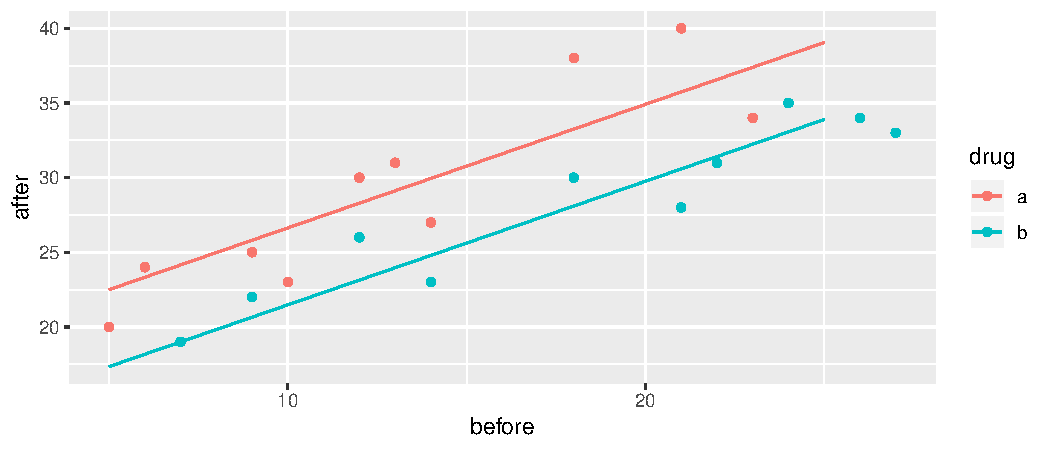
\includegraphics{figure/cabazzo-1.pdf}
\caption{plot of chunk cabazzo}
\end{figure}

Lines now \emph{parallel}. No-interaction model forces them to have the
same slope.

\end{frame}

\begin{frame}[fragile]{Different look at model output}
\protect\hypertarget{different-look-at-model-output}{}

\begin{itemize}
\item
  \texttt{anova(prepost.2)} tests for significant effect of before score
  and of drug, but doesn't help with interpretation.
\item
  \texttt{summary(prepost.2)} views as regression with slopes:
\end{itemize}

\scriptsize

\begin{Shaded}
\begin{Highlighting}[]
\KeywordTok{summary}\NormalTok{(prepost}\FloatTok{.2}\NormalTok{)}
\end{Highlighting}
\end{Shaded}

\begin{verbatim}
## 
## Call:
## lm(formula = after ~ before + drug, data = prepost)
## 
## Residuals:
##     Min      1Q  Median      3Q     Max 
## -3.6348 -2.5099 -0.2038  1.8871  4.7453 
## 
## Coefficients:
##             Estimate Std. Error t value Pr(>|t|)    
## (Intercept)  18.3600     1.5115  12.147 8.35e-10 ***
## before        0.8275     0.0955   8.665 1.21e-07 ***
## drugb        -5.1547     1.2876  -4.003 0.000921 ***
## ---
## Signif. codes:  
## 0 '***' 0.001 '**' 0.01 '*' 0.05 '.' 0.1 ' ' 1
## 
## Residual standard error: 2.682 on 17 degrees of freedom
## Multiple R-squared:  0.817,  Adjusted R-squared:  0.7955 
## F-statistic: 37.96 on 2 and 17 DF,  p-value: 5.372e-07
\end{verbatim}

\normalsize

\end{frame}

\begin{frame}[fragile]{Understanding those slopes}
\protect\hypertarget{understanding-those-slopes}{}

\footnotesize

\begin{Shaded}
\begin{Highlighting}[]
\KeywordTok{tidy}\NormalTok{(prepost}\FloatTok{.2}\NormalTok{)}
\end{Highlighting}
\end{Shaded}

\begin{verbatim}
## # A tibble: 3 x 5
##   term        estimate std.error statistic  p.value
##   <chr>          <dbl>     <dbl>     <dbl>    <dbl>
## 1 (Intercept)   18.4      1.51       12.1  8.35e-10
## 2 before         0.827    0.0955      8.66 1.21e- 7
## 3 drugb         -5.15     1.29       -4.00 9.21e- 4
\end{verbatim}

\normalsize

\begin{itemize}
\item
  \texttt{before} ordinary numerical variable; \texttt{drug}
  categorical.
\item
  \texttt{lm} uses first category \texttt{druga} as baseline.
\item
  Intercept is prediction of after score for before score 0 and
  \emph{drug A}.
\item
  \texttt{before} slope is predicted change in after score when before
  score increases by 1 (usual slope)
\item
  Slope for \texttt{drugb} is \emph{change} in predicted after score for
  being on drug B rather than drug A. Same for \emph{any} before score
  (no interaction).
\end{itemize}

\end{frame}

\begin{frame}{Summary}
\protect\hypertarget{summary}{}

\begin{itemize}
\item
  ANCOVA model: fits different regression line for each group,
  predicting response from covariate.
\item
  ANCOVA model with interaction between factor and covariate allows
  different slopes for each line.
\item
  Sometimes those lines can cross over!
\item
  If interaction not significant, take out. Lines then parallel.
\item
  With parallel lines, groups have consistent effect regardless of value
  of covariate.
\end{itemize}

\end{frame}

\hypertarget{multivariate-anova}{%
\section{Multivariate ANOVA}\label{multivariate-anova}}

\begin{frame}{Multivariate analysis of variance}
\protect\hypertarget{multivariate-analysis-of-variance}{}

\begin{itemize}
\item
  Standard ANOVA has just one response variable.
\item
  What if you have more than one response?
\item
  Try an ANOVA on each response separately.
\item
  But might miss some kinds of interesting dependence between the
  responses that distinguish the groups.
\end{itemize}

\end{frame}

\begin{frame}[fragile]{Packages}
\protect\hypertarget{packages-4}{}

\begin{Shaded}
\begin{Highlighting}[]
\KeywordTok{library}\NormalTok{(car)}
\KeywordTok{library}\NormalTok{(tidyverse)}
\end{Highlighting}
\end{Shaded}

\end{frame}

\begin{frame}[fragile]{Small example}
\protect\hypertarget{small-example}{}

\begin{itemize}
\item
  Measure yield and seed weight of plants grown under 2 conditions: low
  and high amounts of fertilizer.
\item
  Data (fertilizer, yield, seed weight):
\end{itemize}

\begin{Shaded}
\begin{Highlighting}[]
\NormalTok{url <-}\StringTok{ "http://www.utsc.utoronto.ca/~butler/d29/manova1.txt"}
\NormalTok{hilo <-}\StringTok{ }\KeywordTok{read_delim}\NormalTok{(url, }\StringTok{" "}\NormalTok{)}
\end{Highlighting}
\end{Shaded}

\begin{verbatim}
## Parsed with column specification:
## cols(
##   fertilizer = col_character(),
##   yield = col_double(),
##   weight = col_double()
## )
\end{verbatim}

\begin{itemize}
\tightlist
\item
  2 responses, yield and seed weight.
\end{itemize}

\end{frame}

\begin{frame}[fragile]{The data}
\protect\hypertarget{the-data-9}{}

\begin{Shaded}
\begin{Highlighting}[]
\NormalTok{hilo}
\end{Highlighting}
\end{Shaded}

\begin{verbatim}
## # A tibble: 8 x 3
##   fertilizer yield weight
##   <chr>      <dbl>  <dbl>
## 1 low           34     10
## 2 low           29     14
## 3 low           35     11
## 4 low           32     13
## 5 high          33     14
## 6 high          38     12
## 7 high          34     13
## 8 high          35     14
\end{verbatim}

\end{frame}

\begin{frame}[fragile]{Boxplot for yield for each fertilizer group}
\protect\hypertarget{boxplot-for-yield-for-each-fertilizer-group}{}

\begin{Shaded}
\begin{Highlighting}[]
\KeywordTok{ggplot}\NormalTok{(hilo, }\KeywordTok{aes}\NormalTok{(}\DataTypeTok{x =}\NormalTok{ fertilizer, }\DataTypeTok{y =}\NormalTok{ yield)) }\OperatorTok{+}\StringTok{ }\KeywordTok{geom_boxplot}\NormalTok{()}
\end{Highlighting}
\end{Shaded}

\begin{figure}
\centering
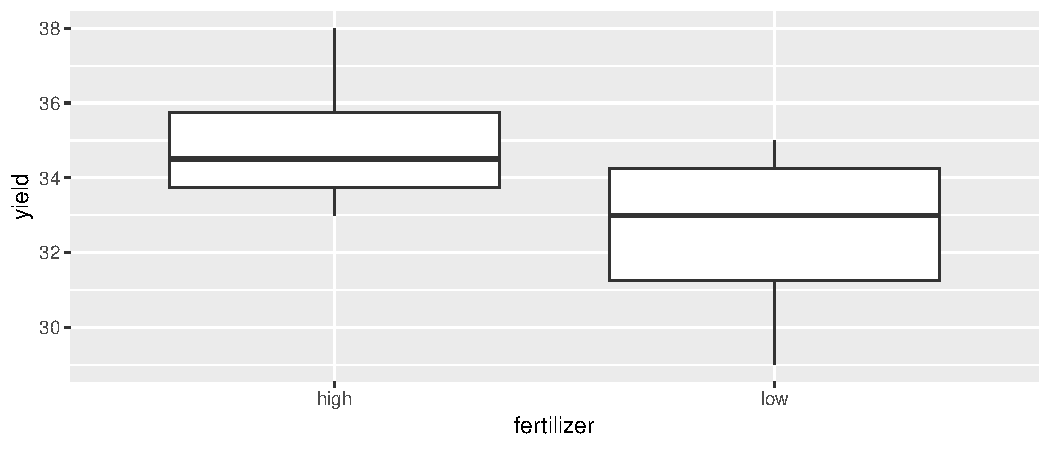
\includegraphics{figure/ferto-1.pdf}
\caption{plot of chunk ferto}
\end{figure}

Yields overlap for fertilizer groups.

\end{frame}

\begin{frame}[fragile]{Boxplot for weight for each fertilizer group}
\protect\hypertarget{boxplot-for-weight-for-each-fertilizer-group}{}

\begin{Shaded}
\begin{Highlighting}[]
\KeywordTok{ggplot}\NormalTok{(hilo, }\KeywordTok{aes}\NormalTok{(}\DataTypeTok{x =}\NormalTok{ fertilizer, }\DataTypeTok{y =}\NormalTok{ weight)) }\OperatorTok{+}\StringTok{ }\KeywordTok{geom_boxplot}\NormalTok{()}
\end{Highlighting}
\end{Shaded}

\begin{figure}
\centering
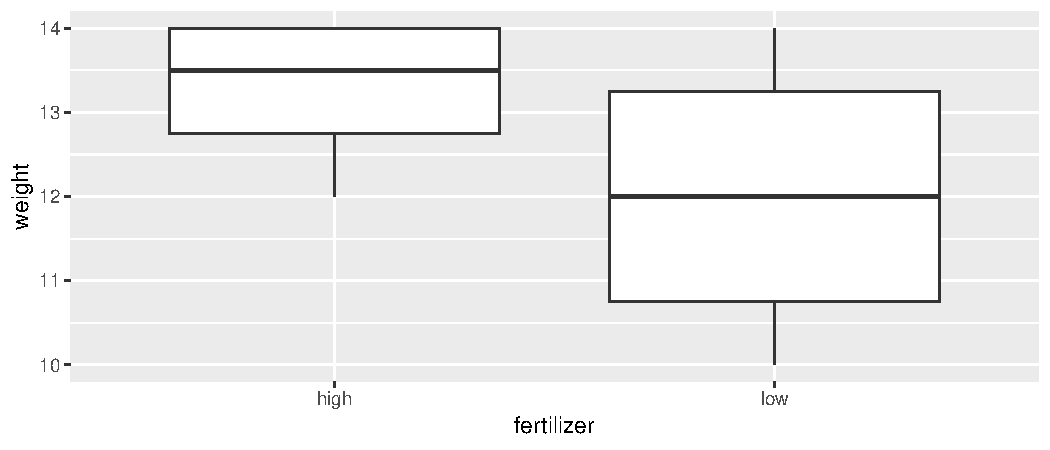
\includegraphics{figure/casteldisangro-1.pdf}
\caption{plot of chunk casteldisangro}
\end{figure}

Weights overlap for fertilizer groups.

\end{frame}

\begin{frame}[fragile]{ANOVAs for yield and weight}
\protect\hypertarget{anovas-for-yield-and-weight}{}

\small

\begin{Shaded}
\begin{Highlighting}[]
\NormalTok{hilo.y <-}\StringTok{ }\KeywordTok{aov}\NormalTok{(yield }\OperatorTok{~}\StringTok{ }\NormalTok{fertilizer, }\DataTypeTok{data =}\NormalTok{ hilo)}
\KeywordTok{summary}\NormalTok{(hilo.y)}
\end{Highlighting}
\end{Shaded}

\begin{verbatim}
##             Df Sum Sq Mean Sq F value Pr(>F)
## fertilizer   1   12.5  12.500   2.143  0.194
## Residuals    6   35.0   5.833
\end{verbatim}

\begin{Shaded}
\begin{Highlighting}[]
\NormalTok{hilo.w <-}\StringTok{ }\KeywordTok{aov}\NormalTok{(weight }\OperatorTok{~}\StringTok{ }\NormalTok{fertilizer, }\DataTypeTok{data =}\NormalTok{ hilo)}
\KeywordTok{summary}\NormalTok{(hilo.w)}
\end{Highlighting}
\end{Shaded}

\begin{verbatim}
##             Df Sum Sq Mean Sq F value Pr(>F)
## fertilizer   1  3.125   3.125   1.471  0.271
## Residuals    6 12.750   2.125
\end{verbatim}

\normalsize

Neither response depends significantly on fertilizer. But\ldots

\end{frame}

\begin{frame}[fragile]{Plotting both responses at once}
\protect\hypertarget{plotting-both-responses-at-once}{}

\begin{itemize}
\item
  Have two response variables (not more), so can plot the response
  variables against \emph{each other}, labelling points by which
  fertilizer group they're from.
\item
  First, create data frame with points \((31,14)\) and \((38,10)\) (why?
  Later):
\end{itemize}

\begin{Shaded}
\begin{Highlighting}[]
\NormalTok{d <-}\StringTok{ }\KeywordTok{tribble}\NormalTok{(}
  \OperatorTok{~}\NormalTok{line_x, }\OperatorTok{~}\NormalTok{line_y,}
  \DecValTok{31}\NormalTok{, }\DecValTok{14}\NormalTok{,}
  \DecValTok{38}\NormalTok{, }\DecValTok{10}
\NormalTok{)}
\end{Highlighting}
\end{Shaded}

\begin{itemize}
\tightlist
\item
  Then plot data as points, and add line through points in \texttt{d}:
\end{itemize}

\begin{Shaded}
\begin{Highlighting}[]
\NormalTok{g <-}\StringTok{ }\KeywordTok{ggplot}\NormalTok{(hilo, }\KeywordTok{aes}\NormalTok{(}\DataTypeTok{x =}\NormalTok{ yield, }\DataTypeTok{y =}\NormalTok{ weight,}
                      \DataTypeTok{colour =}\NormalTok{ fertilizer)) }\OperatorTok{+}\StringTok{ }\KeywordTok{geom_point}\NormalTok{() }\OperatorTok{+}
\StringTok{  }\KeywordTok{geom_line}\NormalTok{(}\DataTypeTok{data =}\NormalTok{ d,}
            \KeywordTok{aes}\NormalTok{(}\DataTypeTok{x =}\NormalTok{ line_x, }\DataTypeTok{y =}\NormalTok{ line_y, }\DataTypeTok{colour =} \OtherTok{NULL}\NormalTok{))}
\end{Highlighting}
\end{Shaded}

\end{frame}

\begin{frame}{The plot}
\protect\hypertarget{the-plot-6}{}

\begin{figure}
\centering
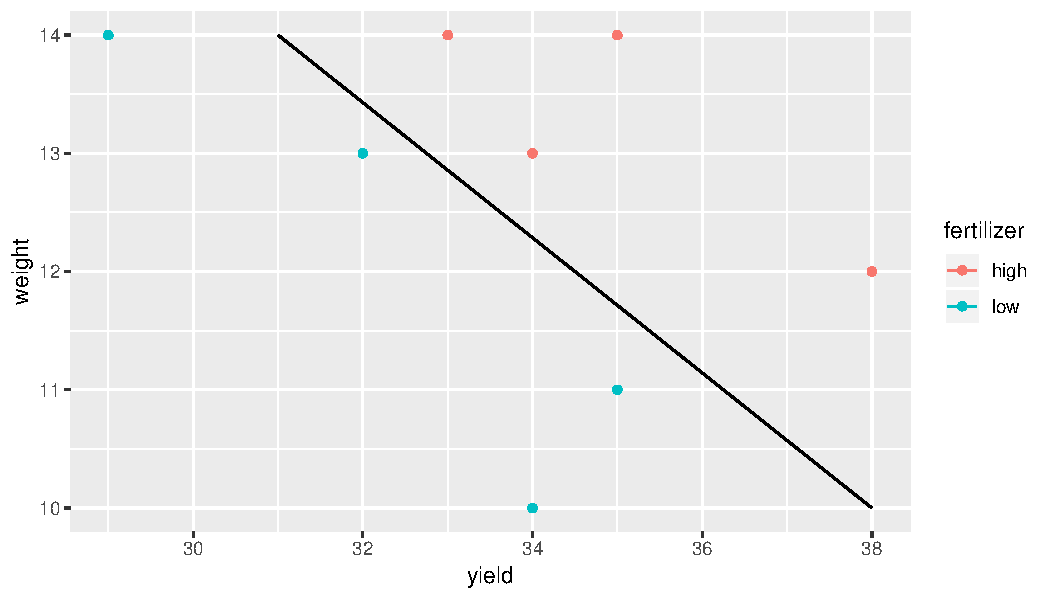
\includegraphics{figure/charlecombe-1.pdf}
\caption{plot of chunk charlecombe}
\end{figure}

\end{frame}

\begin{frame}[fragile]{Comments}
\protect\hypertarget{comments-18}{}

\begin{itemize}
\tightlist
\item
  Graph construction:

  \begin{itemize}
  \tightlist
  \item
    Joining points in \texttt{d} by line.
  \item
    \texttt{geom\_line} inherits \texttt{colour} from \texttt{aes} in
    \texttt{ggplot}.
  \item
    Data frame \texttt{d} has no \texttt{fertilizer} (previous
    \texttt{colour}), so have to unset.
  \end{itemize}
\item
  Results:

  \begin{itemize}
  \item
    High-fertilizer plants have both yield and weight high.
  \item
    True even though no sig difference in yield or weight individually.
  \item
    Drew line separating highs from lows on plot.
  \end{itemize}
\end{itemize}

\end{frame}

\begin{frame}[fragile]{MANOVA finds multivariate differences}
\protect\hypertarget{manova-finds-multivariate-differences}{}

\begin{itemize}
\tightlist
\item
  Is difference found by diagonal line significant? MANOVA finds out.
\end{itemize}

\begin{Shaded}
\begin{Highlighting}[]
\NormalTok{response <-}\StringTok{ }\KeywordTok{with}\NormalTok{(hilo, }\KeywordTok{cbind}\NormalTok{(yield, weight))}
\NormalTok{hilo}\FloatTok{.1}\NormalTok{ <-}\StringTok{ }\KeywordTok{manova}\NormalTok{(response }\OperatorTok{~}\StringTok{ }\NormalTok{fertilizer, }\DataTypeTok{data =}\NormalTok{ hilo)}
\KeywordTok{summary}\NormalTok{(hilo}\FloatTok{.1}\NormalTok{)}
\end{Highlighting}
\end{Shaded}

\begin{verbatim}
##            Df  Pillai approx F num Df den Df  Pr(>F)  
## fertilizer  1 0.80154   10.097      2      5 0.01755 *
## Residuals   6                                         
## ---
## Signif. codes:  
## 0 '***' 0.001 '**' 0.01 '*' 0.05 '.' 0.1 ' ' 1
\end{verbatim}

\begin{itemize}
\tightlist
\item
  Yes! Difference between groups is \emph{diagonally}, not just up/down
  (weight) or left-right (yield). The \emph{yield-weight combination}
  matters.
\end{itemize}

\end{frame}

\begin{frame}[fragile]{Strategy}
\protect\hypertarget{strategy}{}

\begin{itemize}
\item
  Create new response variable by gluing together columns of responses,
  using \texttt{cbind}.
\item
  Use \texttt{manova} with new response, looks like \texttt{lm}
  otherwise.
\item
  With more than 2 responses, cannot draw graph. What then?
\item
  If MANOVA test significant, cannot use Tukey. What then?
\item
  Use \emph{discriminant analysis} (of which more later).
\end{itemize}

\end{frame}

\begin{frame}[fragile]{Another way to do MANOVA}
\protect\hypertarget{another-way-to-do-manova}{}

Install (once) and load package \texttt{car}:

\begin{Shaded}
\begin{Highlighting}[]
\KeywordTok{library}\NormalTok{(car)}
\end{Highlighting}
\end{Shaded}

\end{frame}

\begin{frame}[fragile]{Another way\ldots}
\protect\hypertarget{another-way-1}{}

\begin{Shaded}
\begin{Highlighting}[]
\NormalTok{hilo.}\FloatTok{2.}\NormalTok{lm <-}\StringTok{ }\KeywordTok{lm}\NormalTok{(response }\OperatorTok{~}\StringTok{ }\NormalTok{fertilizer, }\DataTypeTok{data =}\NormalTok{ hilo)}
\NormalTok{hilo}\FloatTok{.2}\NormalTok{ <-}\StringTok{ }\KeywordTok{Manova}\NormalTok{(hilo.}\FloatTok{2.}\NormalTok{lm)}
\NormalTok{hilo}\FloatTok{.2}
\end{Highlighting}
\end{Shaded}

\begin{verbatim}
## 
## Type II MANOVA Tests: Pillai test statistic
##            Df test stat approx F num Df den Df  Pr(>F)  
## fertilizer  1   0.80154   10.097      2      5 0.01755 *
## ---
## Signif. codes:  
## 0 '***' 0.001 '**' 0.01 '*' 0.05 '.' 0.1 ' ' 1
\end{verbatim}

\begin{itemize}
\item
  Same result as small-m \texttt{manova}.
\item
  \texttt{Manova} will also do \emph{repeated measures}, coming up
  later.
\end{itemize}

\end{frame}

\begin{frame}[fragile]{Another example: peanuts}
\protect\hypertarget{another-example-peanuts}{}

\begin{itemize}
\item
  Three different varieties of peanuts (mysteriously, 5, 6 and 8)
  planted in two different locations.
\item
  Three response variables: \texttt{y}, \texttt{smk} and \texttt{w}.
\end{itemize}

\begin{Shaded}
\begin{Highlighting}[]
\NormalTok{u <-}\StringTok{ "http://www.utsc.utoronto.ca/~butler/d29/peanuts.txt"}
\NormalTok{peanuts.orig <-}\StringTok{ }\KeywordTok{read_delim}\NormalTok{(u, }\StringTok{" "}\NormalTok{)}
\end{Highlighting}
\end{Shaded}

\begin{verbatim}
## Parsed with column specification:
## cols(
##   obs = col_double(),
##   location = col_double(),
##   variety = col_double(),
##   y = col_double(),
##   smk = col_double(),
##   w = col_double()
## )
\end{verbatim}

\end{frame}

\begin{frame}[fragile]{The data}
\protect\hypertarget{the-data-10}{}

\small

\begin{Shaded}
\begin{Highlighting}[]
\NormalTok{peanuts.orig}
\end{Highlighting}
\end{Shaded}

\begin{verbatim}
## # A tibble: 12 x 6
##      obs location variety     y   smk     w
##    <dbl>    <dbl>   <dbl> <dbl> <dbl> <dbl>
##  1     1        1       5  195.  153.  51.4
##  2     2        1       5  194.  168.  53.7
##  3     3        2       5  190.  140.  55.5
##  4     4        2       5  180.  121.  44.4
##  5     5        1       6  203   157.  49.8
##  6     6        1       6  196.  166   45.8
##  7     7        2       6  203.  166.  60.4
##  8     8        2       6  198.  162.  54.1
##  9     9        1       8  194.  164.  57.8
## 10    10        1       8  187   165.  58.6
## 11    11        2       8  202.  167.  65  
## 12    12        2       8  200   174.  67.2
\end{verbatim}

\normalsize

\end{frame}

\begin{frame}[fragile]{Setup for analysis}
\protect\hypertarget{setup-for-analysis}{}

\begin{Shaded}
\begin{Highlighting}[]
\NormalTok{peanuts <-}\StringTok{ }\NormalTok{peanuts.orig }\OperatorTok
\StringTok{  }\KeywordTok{mutate}\NormalTok{(}
    \DataTypeTok{location =} \KeywordTok{factor}\NormalTok{(location),}
    \DataTypeTok{variety =} \KeywordTok{factor}\NormalTok{(variety)}
\NormalTok{  )}
\NormalTok{response <-}\StringTok{ }\KeywordTok{with}\NormalTok{(peanuts, }\KeywordTok{cbind}\NormalTok{(y, smk, w))}
\KeywordTok{head}\NormalTok{(response)}
\end{Highlighting}
\end{Shaded}

\begin{verbatim}
##          y   smk    w
## [1,] 195.3 153.1 51.4
## [2,] 194.3 167.7 53.7
## [3,] 189.7 139.5 55.5
## [4,] 180.4 121.1 44.4
## [5,] 203.0 156.8 49.8
## [6,] 195.9 166.0 45.8
\end{verbatim}

\end{frame}

\begin{frame}[fragile]{Analysis (using \texttt{Manova)}}
\protect\hypertarget{analysis-using-manova}{}

\small

\begin{Shaded}
\begin{Highlighting}[]
\NormalTok{peanuts}\FloatTok{.1}\NormalTok{ <-}\StringTok{ }\KeywordTok{lm}\NormalTok{(response }\OperatorTok{~}\StringTok{ }\NormalTok{location }\OperatorTok{*}\StringTok{ }\NormalTok{variety, }\DataTypeTok{data =}\NormalTok{ peanuts)}
\NormalTok{peanuts}\FloatTok{.2}\NormalTok{ <-}\StringTok{ }\KeywordTok{Manova}\NormalTok{(peanuts}\FloatTok{.1}\NormalTok{)}
\NormalTok{peanuts}\FloatTok{.2}
\end{Highlighting}
\end{Shaded}

\begin{verbatim}
## 
## Type II MANOVA Tests: Pillai test statistic
##                  Df test stat approx F num Df den Df
## location          1   0.89348  11.1843      3      4
## variety           2   1.70911   9.7924      6     10
## location:variety  2   1.29086   3.0339      6     10
##                    Pr(>F)   
## location         0.020502 * 
## variety          0.001056 **
## location:variety 0.058708 . 
## ---
## Signif. codes:  
## 0 '***' 0.001 '**' 0.01 '*' 0.05 '.' 0.1 ' ' 1
\end{verbatim}

\normalsize

\end{frame}

\begin{frame}[fragile]{Comments}
\protect\hypertarget{comments-19}{}

\begin{itemize}
\item
  Interaction not quite significant, but main effects are.
\item
  Combined response variable \texttt{(y,smk,w)} definitely depends on
  location and on variety
\item
  Weak dependence of \texttt{(y,smk,w)} on the location-variety
  \emph{combination.}
\item
  Understanding that dependence beyond our scope right now.
\end{itemize}

\end{frame}

\hypertarget{repeated-measures-by-profile-analysis}{%
\section{Repeated measures by profile
analysis}\label{repeated-measures-by-profile-analysis}}

\begin{frame}[fragile]{Repeated measures by profile analysis}
\protect\hypertarget{repeated-measures-by-profile-analysis-1}{}

\begin{itemize}
\item
  More than one response \emph{measurement} for each subject. Might be
\item
  measurements of the same thing at different times
\item
  measurements of different but related things
\item
  Generalization of matched pairs (``matched triples'', etc.).
\item
  Variation: each subject does several different treatments at different
  times (called \emph{crossover design}).
\item
  Expect measurements on same subject to be correlated, so assumptions
  of independence will fail.
\item
  Called \emph{repeated measures}. Different approaches, but
  \emph{profile analysis} uses \texttt{Manova} (set up right way).
\item
  Another approach uses \emph{mixed models} (random effects).
\end{itemize}

\end{frame}

\begin{frame}[fragile]{Packages}
\protect\hypertarget{packages-5}{}

\begin{Shaded}
\begin{Highlighting}[]
\KeywordTok{library}\NormalTok{(car)}
\KeywordTok{library}\NormalTok{(tidyverse)}
\end{Highlighting}
\end{Shaded}

\end{frame}

\begin{frame}[fragile]{Example: histamine in dogs}
\protect\hypertarget{example-histamine-in-dogs}{}

\begin{itemize}
\item
  8 dogs take part in experiment.
\item
  Dogs randomized to one of 2 different drugs.
\item
  Response: log of blood concentration of histamine 0, 1, 3 and 5
  minutes after taking drug. (Repeated measures.)
\item
  Data in \texttt{dogs.txt}, column-aligned.
\end{itemize}

\end{frame}

\begin{frame}[fragile]{Read in data}
\protect\hypertarget{read-in-data-3}{}

\begin{Shaded}
\begin{Highlighting}[]
\NormalTok{my_url <-}\StringTok{ "http://www.utsc.utoronto.ca/~butler/d29/dogs.txt"}
\NormalTok{dogs <-}\StringTok{ }\KeywordTok{read_table}\NormalTok{(my_url)}
\end{Highlighting}
\end{Shaded}

\begin{verbatim}
## Parsed with column specification:
## cols(
##   dog = col_character(),
##   drug = col_character(),
##   x = col_character(),
##   lh0 = col_double(),
##   lh1 = col_double(),
##   lh3 = col_double(),
##   lh5 = col_double()
## )
\end{verbatim}

\end{frame}

\begin{frame}[fragile]{Setting things up}
\protect\hypertarget{setting-things-up}{}

\begin{Shaded}
\begin{Highlighting}[]
\NormalTok{dogs}
\end{Highlighting}
\end{Shaded}

\begin{verbatim}
## # A tibble: 8 x 7
##   dog   drug         x       lh0   lh1   lh3   lh5
##   <chr> <chr>        <chr> <dbl> <dbl> <dbl> <dbl>
## 1 A     Morphine     N     -3.22 -1.61 -2.3  -2.53
## 2 B     Morphine     N     -3.91 -2.81 -3.91 -3.91
## 3 C     Morphine     N     -2.66  0.34 -0.73 -1.43
## 4 D     Morphine     N     -1.77 -0.56 -1.05 -1.43
## 5 E     Trimethaphan N     -3.51 -0.48 -1.17 -1.51
## 6 F     Trimethaphan N     -3.51  0.05 -0.31 -0.51
## 7 G     Trimethaphan N     -2.66 -0.19  0.07 -0.22
## 8 H     Trimethaphan N     -2.41  1.14  0.72  0.21
\end{verbatim}

\begin{Shaded}
\begin{Highlighting}[]
\NormalTok{response <-}\StringTok{ }\KeywordTok{with}\NormalTok{(dogs, }\KeywordTok{cbind}\NormalTok{(lh0, lh1, lh3, lh5))}
\NormalTok{dogs}\FloatTok{.1}\NormalTok{ <-}\StringTok{ }\KeywordTok{lm}\NormalTok{(response }\OperatorTok{~}\StringTok{ }\NormalTok{drug, }\DataTypeTok{data =}\NormalTok{ dogs)}
\end{Highlighting}
\end{Shaded}

\end{frame}

\begin{frame}[fragile]{The repeated measures MANOVA}
\protect\hypertarget{the-repeated-measures-manova}{}

Get list of response variable names; we call them \texttt{times}. Save
in data frame.

\footnotesize

\begin{Shaded}
\begin{Highlighting}[]
\NormalTok{times <-}\StringTok{ }\KeywordTok{colnames}\NormalTok{(response)}
\NormalTok{times.df <-}\StringTok{ }\KeywordTok{data.frame}\NormalTok{(times)}
\NormalTok{dogs}\FloatTok{.2}\NormalTok{ <-}\StringTok{ }\KeywordTok{Manova}\NormalTok{(dogs}\FloatTok{.1}\NormalTok{,}
  \DataTypeTok{idata =}\NormalTok{ times.df,}
  \DataTypeTok{idesign =} \OperatorTok{~}\NormalTok{times}
\NormalTok{)}
\NormalTok{dogs}\FloatTok{.2}
\end{Highlighting}
\end{Shaded}

\begin{verbatim}
## 
## Type II Repeated Measures MANOVA Tests: Pillai test statistic
##             Df test stat approx F num Df den Df   Pr(>F)   
## (Intercept)  1   0.76347  19.3664      1      6 0.004565 **
## drug         1   0.34263   3.1272      1      6 0.127406   
## times        1   0.94988  25.2690      3      4 0.004631 **
## drug:times   1   0.89476  11.3362      3      4 0.020023 * 
## ---
## Signif. codes:  
## 0 '***' 0.001 '**' 0.01 '*' 0.05 '.' 0.1 ' ' 1
\end{verbatim}

\normalsize

\end{frame}

\begin{frame}{Wide and long format}
\protect\hypertarget{wide-and-long-format}{}

\begin{itemize}
\item
  Interaction significant. Pattern of response over time different for
  the two drugs.
\item
  Want to investigate interaction.
\end{itemize}

\end{frame}

\begin{frame}[fragile]{The wrong shape}
\protect\hypertarget{the-wrong-shape}{}

\begin{itemize}
\tightlist
\item
  But data frame has several observations per line (``wide format''):
\end{itemize}

\scriptsize

\begin{Shaded}
\begin{Highlighting}[]
\NormalTok{dogs }\OperatorTok\StringTok{ }\KeywordTok{slice}\NormalTok{(}\DecValTok{1}\OperatorTok{:}\DecValTok{6}\NormalTok{)}
\end{Highlighting}
\end{Shaded}

\begin{verbatim}
## # A tibble: 6 x 7
##   dog   drug         x       lh0   lh1   lh3   lh5
##   <chr> <chr>        <chr> <dbl> <dbl> <dbl> <dbl>
## 1 A     Morphine     N     -3.22 -1.61 -2.3  -2.53
## 2 B     Morphine     N     -3.91 -2.81 -3.91 -3.91
## 3 C     Morphine     N     -2.66  0.34 -0.73 -1.43
## 4 D     Morphine     N     -1.77 -0.56 -1.05 -1.43
## 5 E     Trimethaphan N     -3.51 -0.48 -1.17 -1.51
## 6 F     Trimethaphan N     -3.51  0.05 -0.31 -0.51
\end{verbatim}

\normalsize

\begin{itemize}
\item
  Plotting works with data in ``long format'': one response per line.
\item
  The responses are log-histamine at different times, labelled
  \texttt{lh}-something. Call them all \texttt{lh} and put them in one
  column, with the time they belong to labelled.
\end{itemize}

\end{frame}

\begin{frame}[fragile]{Running \texttt{gather}, try 1}
\protect\hypertarget{running-gather-try-1}{}

\footnotesize

\begin{Shaded}
\begin{Highlighting}[]
\NormalTok{dogs }\OperatorTok\StringTok{ }\KeywordTok{gather}\NormalTok{(time, lh, lh0}\OperatorTok{:}\NormalTok{lh5) }
\end{Highlighting}
\end{Shaded}

\begin{verbatim}
## # A tibble: 32 x 5
##    dog   drug         x     time     lh
##    <chr> <chr>        <chr> <chr> <dbl>
##  1 A     Morphine     N     lh0   -3.22
##  2 B     Morphine     N     lh0   -3.91
##  3 C     Morphine     N     lh0   -2.66
##  4 D     Morphine     N     lh0   -1.77
##  5 E     Trimethaphan N     lh0   -3.51
##  6 F     Trimethaphan N     lh0   -3.51
##  7 G     Trimethaphan N     lh0   -2.66
##  8 H     Trimethaphan N     lh0   -2.41
##  9 A     Morphine     N     lh1   -1.61
## 10 B     Morphine     N     lh1   -2.81
## # … with 22 more rows
\end{verbatim}

\normalsize

\end{frame}

\begin{frame}[fragile]{Getting the times}
\protect\hypertarget{getting-the-times}{}

Not quite right: for the times, we want just the numbers, not the
letters \texttt{lh} every time. Want new variable containing just number
in \texttt{time}: \texttt{parse\_number}.

\footnotesize

\begin{Shaded}
\begin{Highlighting}[]
\NormalTok{dogs }\OperatorTok
\StringTok{  }\KeywordTok{gather}\NormalTok{(timex, lh, lh0}\OperatorTok{:}\NormalTok{lh5) }\OperatorTok
\StringTok{  }\KeywordTok{mutate}\NormalTok{(}\DataTypeTok{time =} \KeywordTok{parse_number}\NormalTok{(timex)) }
\end{Highlighting}
\end{Shaded}

\begin{verbatim}
## # A tibble: 32 x 6
##    dog   drug         x     timex    lh  time
##    <chr> <chr>        <chr> <chr> <dbl> <dbl>
##  1 A     Morphine     N     lh0   -3.22     0
##  2 B     Morphine     N     lh0   -3.91     0
##  3 C     Morphine     N     lh0   -2.66     0
##  4 D     Morphine     N     lh0   -1.77     0
##  5 E     Trimethaphan N     lh0   -3.51     0
##  6 F     Trimethaphan N     lh0   -3.51     0
##  7 G     Trimethaphan N     lh0   -2.66     0
##  8 H     Trimethaphan N     lh0   -2.41     0
##  9 A     Morphine     N     lh1   -1.61     1
## 10 B     Morphine     N     lh1   -2.81     1
## # … with 22 more rows
\end{verbatim}

\normalsize

\end{frame}

\begin{frame}[fragile]{What I did differently}
\protect\hypertarget{what-i-did-differently}{}

\begin{itemize}
\item
  I realized that \texttt{gather} was going to produce something like
  \texttt{lh1}, which I needed to do something further with, so this
  time I gave it a temporary name \texttt{timex}.
\item
  This enabled me to use the name \texttt{time} for the actual numeric
  time.
\item
  This works now, so next save into a new data frame \texttt{dogs.long}.
\end{itemize}

\end{frame}

\begin{frame}[fragile]{Saving the pipelined results}
\protect\hypertarget{saving-the-pipelined-results}{}

\begin{Shaded}
\begin{Highlighting}[]
\NormalTok{dogs }\OperatorTok
\StringTok{  }\KeywordTok{gather}\NormalTok{(timex, lh, lh0}\OperatorTok{:}\NormalTok{lh5) }\OperatorTok
\StringTok{  }\KeywordTok{mutate}\NormalTok{(}\DataTypeTok{time =} \KeywordTok{parse_number}\NormalTok{(timex)) ->}\StringTok{ }\NormalTok{dogs.long}
\end{Highlighting}
\end{Shaded}

This says:

\begin{itemize}
\item
  Take data frame dogs, and then:
\item
  Combine the columns \texttt{lh0} through \texttt{lh5} into one column
  called \texttt{lh}, with the column that each \texttt{lh} value
  originally came from labelled by \texttt{timex}, and then:
\item
  Pull out numeric values in \texttt{timex}, saving in \texttt{time} and
  then:
\item
  save the result in a data frame \texttt{dogs.long}.
\end{itemize}

\end{frame}

\begin{frame}[fragile]{Interaction plot}
\protect\hypertarget{interaction-plot-3}{}

\small

\begin{Shaded}
\begin{Highlighting}[]
\KeywordTok{ggplot}\NormalTok{(dogs.long, }\KeywordTok{aes}\NormalTok{(}\DataTypeTok{x =}\NormalTok{ time, }\DataTypeTok{y =}\NormalTok{ lh, }
                      \DataTypeTok{colour =}\NormalTok{ drug, }\DataTypeTok{group =}\NormalTok{ drug)) }\OperatorTok{+}
\StringTok{  }\KeywordTok{stat_summary}\NormalTok{(}\DataTypeTok{fun.y =}\NormalTok{ mean, }\DataTypeTok{geom =} \StringTok{"point"}\NormalTok{) }\OperatorTok{+}
\StringTok{  }\KeywordTok{stat_summary}\NormalTok{(}\DataTypeTok{fun.y =}\NormalTok{ mean, }\DataTypeTok{geom =} \StringTok{"line"}\NormalTok{)}
\end{Highlighting}
\end{Shaded}

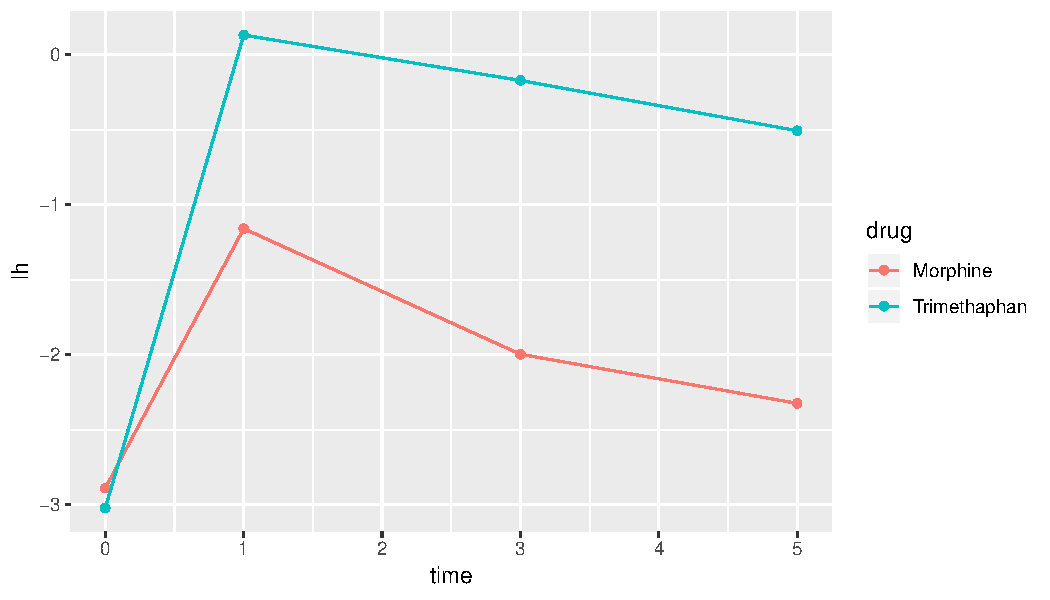
\includegraphics{figure/unnamed-chunk-250-1.pdf} \normalsize

\end{frame}

\begin{frame}[fragile]{Comments}
\protect\hypertarget{comments-20}{}

\begin{itemize}
\item
  Plot mean \texttt{lh} value at each time, joining points on same drug
  by lines.
\item
  drugs same at time 0
\item
  after that, Trimethaphan higher than Morphine.
\item
  Effect of drug not consistent over time: significant interaction.
\end{itemize}

\end{frame}

\begin{frame}[fragile]{Take out time zero}
\protect\hypertarget{take-out-time-zero}{}

\begin{itemize}
\item
  Lines on interaction plot would then be parallel, and so interaction
  should no longer be significant.
\item
  Go back to original ``wide'' \texttt{dogs} data frame.
\end{itemize}

\begin{Shaded}
\begin{Highlighting}[]
\NormalTok{response <-}\StringTok{ }\KeywordTok{with}\NormalTok{(dogs, }\KeywordTok{cbind}\NormalTok{(lh1, lh3, lh5)) }\CommentTok{# excl time 0}
\NormalTok{dogs}\FloatTok{.1}\NormalTok{ <-}\StringTok{ }\KeywordTok{lm}\NormalTok{(response }\OperatorTok{~}\StringTok{ }\NormalTok{drug, }\DataTypeTok{data =}\NormalTok{ dogs)}
\NormalTok{times <-}\StringTok{ }\KeywordTok{colnames}\NormalTok{(response)}
\NormalTok{times.df <-}\StringTok{ }\KeywordTok{data.frame}\NormalTok{(times)}
\NormalTok{dogs}\FloatTok{.2}\NormalTok{ <-}\StringTok{ }\KeywordTok{Manova}\NormalTok{(dogs}\FloatTok{.1}\NormalTok{,}
  \DataTypeTok{idata =}\NormalTok{ times.df,}
  \DataTypeTok{idesign =} \OperatorTok{~}\NormalTok{times}
\NormalTok{)}
\end{Highlighting}
\end{Shaded}

\end{frame}

\begin{frame}[fragile]{Results and comments}
\protect\hypertarget{results-and-comments}{}

\footnotesize

\begin{Shaded}
\begin{Highlighting}[]
\NormalTok{dogs}\FloatTok{.2}
\end{Highlighting}
\end{Shaded}

\begin{verbatim}
## 
## Type II Repeated Measures MANOVA Tests: Pillai test statistic
##             Df test stat approx F num Df den Df   Pr(>F)   
## (Intercept)  1   0.54582   7.2106      1      6 0.036281 * 
## drug         1   0.44551   4.8207      1      6 0.070527 . 
## times        1   0.85429  14.6569      2      5 0.008105 **
## drug:times   1   0.43553   1.9289      2      5 0.239390   
## ---
## Signif. codes:  
## 0 '***' 0.001 '**' 0.01 '*' 0.05 '.' 0.1 ' ' 1
\end{verbatim}

\normalsize

\begin{itemize}
\item
  Correct: interaction no longer significant.
\item
  Significant effect of time.
\item
  Drug effect not quite significant (some variety among dogs within
  drug).
\end{itemize}

\end{frame}

\begin{frame}[fragile]{Is the non-significant drug effect reasonable?}
\protect\hypertarget{is-the-non-significant-drug-effect-reasonable}{}

\begin{itemize}
\item
  Plot \emph{actual data}: \texttt{lh} against \texttt{days}, labelling
  observations by drug: ``spaghetti plot''.
\item
  Uses long data frame (confusing, yes I know):
\item
  Plot (time,lh) points coloured by drug
\item
  and connecting measurements for each \emph{dog} by lines.
\item
  This time, we want \texttt{group=dog} (want the measurements for each
  \emph{dog} joined by lines), but \texttt{colour=drug}:
\end{itemize}

\begin{Shaded}
\begin{Highlighting}[]
\NormalTok{g <-}\StringTok{ }\KeywordTok{ggplot}\NormalTok{(dogs.long, }\KeywordTok{aes}\NormalTok{(}
  \DataTypeTok{x =}\NormalTok{ time, }\DataTypeTok{y =}\NormalTok{ lh,}
  \DataTypeTok{colour =}\NormalTok{ drug, }\DataTypeTok{group =}\NormalTok{ dog}
\NormalTok{)) }\OperatorTok{+}
\StringTok{  }\KeywordTok{geom_point}\NormalTok{() }\OperatorTok{+}\StringTok{ }\KeywordTok{geom_line}\NormalTok{()}
\end{Highlighting}
\end{Shaded}

\end{frame}

\begin{frame}[fragile]{The spaghetti plot}
\protect\hypertarget{the-spaghetti-plot}{}

\begin{Shaded}
\begin{Highlighting}[]
\NormalTok{g}
\end{Highlighting}
\end{Shaded}

\begin{figure}
\centering
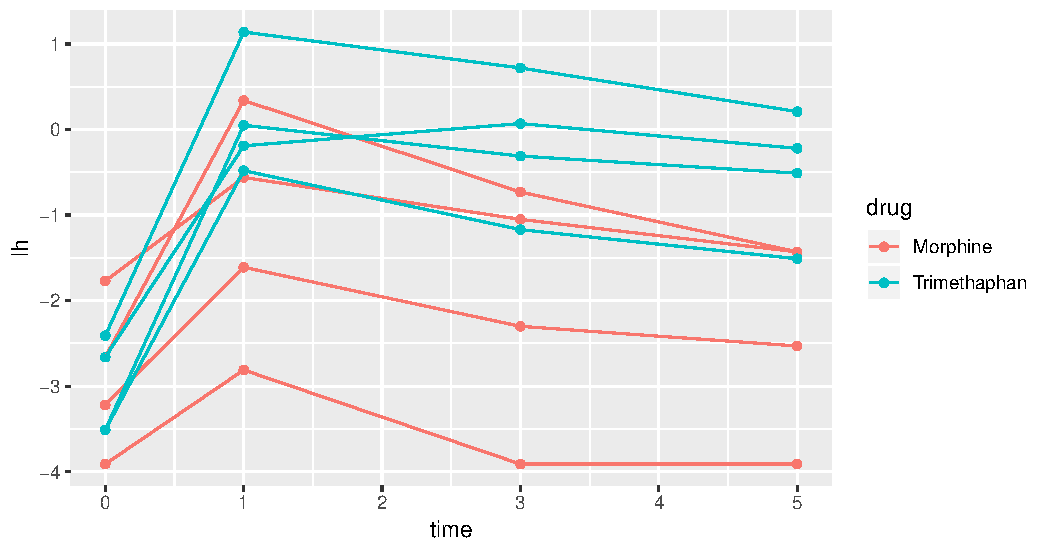
\includegraphics{figure/hoverla-1.pdf}
\caption{plot of chunk hoverla}
\end{figure}

\end{frame}

\begin{frame}[fragile]{Comments}
\protect\hypertarget{comments-21}{}

\begin{itemize}
\item
  For each dog over time, there is a strong increase and gradual
  decrease in log-histamine. This explains the significant time effect.
\item
  The pattern is more or less the same for each dog, regardless of drug.
  This explains the non-significant interaction.
\item
  Most of the trimethaphan dogs (blue) have higher log-histamine
  throughout (time 1 and after), and some of the morphine dogs have
  lower.
\item
  \emph{But} two of the morphine dogs have log-histamine profiles like
  the trimethaphan dogs. This ambiguity is probably why the
  \texttt{drug} effect is not quite significant.
\end{itemize}

\end{frame}

\begin{frame}{The exercise data}
\protect\hypertarget{the-exercise-data}{}

\begin{itemize}
\item
  30 people took part in an exercise study.
\item
  Each subject was randomly assigned to one of two diets (``low fat'' or
  ``non-low fat'') and to one of three exercise programs (``at rest'',
  ``walking'', ``running'').
\item
  There are \(2\times3 = 6\) experimental treatments, and thus each one
  is replicated \(30/6=5\) times.
\item
  Nothing unusual so far.
\item
  However, each subject had their pulse rate measured at three different
  times (1, 15 and 30 minutes after starting their exercise), so have
  repeated measures.
\end{itemize}

\end{frame}

\begin{frame}[fragile]{Reading the data}
\protect\hypertarget{reading-the-data-1}{}

Separated by \emph{tabs}:

\begin{Shaded}
\begin{Highlighting}[]
\NormalTok{url <-}\StringTok{ "http://www.utsc.utoronto.ca/~butler/d29/exercise.txt"}
\NormalTok{exercise.long <-}\StringTok{ }\KeywordTok{read_tsv}\NormalTok{(url)}
\end{Highlighting}
\end{Shaded}

\begin{verbatim}
## Parsed with column specification:
## cols(
##   id = col_double(),
##   diet = col_character(),
##   exertype = col_character(),
##   pulse = col_double(),
##   time = col_character()
## )
\end{verbatim}

\end{frame}

\begin{frame}[fragile]{The data}
\protect\hypertarget{the-data-11}{}

\footnotesize

\begin{Shaded}
\begin{Highlighting}[]
\NormalTok{exercise.long }\OperatorTok\StringTok{ }\KeywordTok{slice}\NormalTok{(}\DecValTok{1}\OperatorTok{:}\DecValTok{8}\NormalTok{)}
\end{Highlighting}
\end{Shaded}

\begin{verbatim}
## # A tibble: 8 x 5
##      id diet      exertype pulse time 
##   <dbl> <chr>     <chr>    <dbl> <chr>
## 1     1 nonlowfat atrest      85 min01
## 2     1 nonlowfat atrest      85 min15
## 3     1 nonlowfat atrest      88 min30
## 4     2 nonlowfat atrest      90 min01
## 5     2 nonlowfat atrest      92 min15
## 6     2 nonlowfat atrest      93 min30
## 7     3 nonlowfat atrest      97 min01
## 8     3 nonlowfat atrest      97 min15
\end{verbatim}

\normalsize

\begin{itemize}
\item
  This is ``long format'', which is usually what we want.
\item
  But for repeated measures analysis, we want \emph{wide} format!
\item
  ``undo'' gather: \texttt{spread}.
\end{itemize}

\end{frame}

\begin{frame}[fragile]{Making wide format}
\protect\hypertarget{making-wide-format}{}

\begin{itemize}
\tightlist
\item
  \texttt{spread} needs: a column that is going to be split, and the
  column to make the values out of:
\end{itemize}

\footnotesize

\begin{Shaded}
\begin{Highlighting}[]
\NormalTok{exercise.long }\OperatorTok\StringTok{ }\KeywordTok{spread}\NormalTok{(time, pulse) ->}\StringTok{ }\NormalTok{exercise.wide}
\NormalTok{exercise.wide }\OperatorTok\StringTok{ }\KeywordTok{sample_n}\NormalTok{(}\DecValTok{5}\NormalTok{)}
\end{Highlighting}
\end{Shaded}

\begin{verbatim}
## # A tibble: 5 x 6
##      id diet      exertype min01 min15 min30
##   <dbl> <chr>     <chr>    <dbl> <dbl> <dbl>
## 1    30 lowfat    running     99   111   150
## 2    10 lowfat    atrest     100    97   100
## 3    20 lowfat    walking    102   104   103
## 4     4 nonlowfat atrest      80    82    83
## 5     7 lowfat    atrest      87    88    90
\end{verbatim}

\normalsize

\begin{itemize}
\tightlist
\item
  Normally \texttt{gather} \texttt{min01, min15,
  min30} into one column called \texttt{pulse} labelled by the number of
  minutes. But \texttt{Manova} needs it the other way.
\end{itemize}

\end{frame}

\begin{frame}[fragile]{Setting up the repeated-measures analysis}
\protect\hypertarget{setting-up-the-repeated-measures-analysis}{}

\begin{itemize}
\tightlist
\item
  Make a response variable consisting of \texttt{min01,\ min15,\ min30}:
\end{itemize}

\small

\begin{Shaded}
\begin{Highlighting}[]
\NormalTok{response <-}\StringTok{ }\KeywordTok{with}\NormalTok{(exercise.wide, }\KeywordTok{cbind}\NormalTok{(min01, min15, min30))}
\end{Highlighting}
\end{Shaded}

\normalsize

\begin{itemize}
\tightlist
\item
  Predict that from \texttt{diet} and \texttt{exertype} and interaction
  using \texttt{lm}:
\end{itemize}

\small

\begin{Shaded}
\begin{Highlighting}[]
\NormalTok{exercise}\FloatTok{.1}\NormalTok{ <-}\StringTok{ }\KeywordTok{lm}\NormalTok{(response }\OperatorTok{~}\StringTok{ }\NormalTok{diet }\OperatorTok{*}\StringTok{ }\NormalTok{exertype,}
  \DataTypeTok{data =}\NormalTok{ exercise.wide}
\NormalTok{)}
\end{Highlighting}
\end{Shaded}

\normalsize

\begin{itemize}
\tightlist
\item
  Run this through \texttt{Manova}:
\end{itemize}

\small

\begin{Shaded}
\begin{Highlighting}[]
\NormalTok{times <-}\StringTok{ }\KeywordTok{colnames}\NormalTok{(response)}
\NormalTok{times.df <-}\StringTok{ }\KeywordTok{data.frame}\NormalTok{(times)}
\NormalTok{exercise}\FloatTok{.2}\NormalTok{ <-}\StringTok{ }\KeywordTok{Manova}\NormalTok{(exercise}\FloatTok{.1}\NormalTok{, }
                     \DataTypeTok{idata =}\NormalTok{ times.df, }
                     \DataTypeTok{idesign =} \OperatorTok{~}\NormalTok{times)}
\end{Highlighting}
\end{Shaded}

\normalsize

\end{frame}

\begin{frame}[fragile]{Results}
\protect\hypertarget{results-1}{}

\scriptsize

\begin{Shaded}
\begin{Highlighting}[]
\NormalTok{exercise}\FloatTok{.2}
\end{Highlighting}
\end{Shaded}

\begin{verbatim}
## 
## Type II Repeated Measures MANOVA Tests: Pillai test statistic
##                     Df test stat approx F num Df den Df    Pr(>F)    
## (Intercept)          1   0.99767  10296.7      1     24 < 2.2e-16 ***
## diet                 1   0.37701     14.5      1     24 0.0008483 ***
## exertype             2   0.79972     47.9      2     24 4.166e-09 ***
## diet:exertype        2   0.28120      4.7      2     24 0.0190230 *  
## times                1   0.78182     41.2      2     23 2.491e-08 ***
## diet:times           1   0.25153      3.9      2     23 0.0357258 *  
## exertype:times       2   0.83557      8.6      4     48 2.538e-05 ***
## diet:exertype:times  2   0.51750      4.2      4     48 0.0054586 ** 
## ---
## Signif. codes:  0 '***' 0.001 '**' 0.01 '*' 0.05 '.' 0.1 ' ' 1
\end{verbatim}

\normalsize

\begin{itemize}
\item
  Three-way interaction significant, so cannot remove anything.
\item
  Pulse rate depends on diet and exercise type \emph{combination}, and
  \emph{that} is different for each time.
\end{itemize}

\end{frame}

\begin{frame}[fragile]{Making some graphs}
\protect\hypertarget{making-some-graphs}{}

\begin{itemize}
\item
  Three-way interactions are difficult to understand. To make an
  attempt, look at some graphs.
\item
  Plot time trace of pulse rates for each individual, joined by lines,
  and make \emph{separate} plots for each \texttt{diet-exertype} combo.
\item
  \texttt{ggplot} again. Using \emph{long} data frame:
\end{itemize}

\begin{Shaded}
\begin{Highlighting}[]
\NormalTok{g <-}\StringTok{ }\KeywordTok{ggplot}\NormalTok{(exercise.long, }\KeywordTok{aes}\NormalTok{(}
  \DataTypeTok{x =}\NormalTok{ time, }\DataTypeTok{y =}\NormalTok{ pulse,}
  \DataTypeTok{group =}\NormalTok{ id}
\NormalTok{)) }\OperatorTok{+}\StringTok{ }\KeywordTok{geom_point}\NormalTok{() }\OperatorTok{+}\StringTok{ }\KeywordTok{geom_line}\NormalTok{() }\OperatorTok{+}
\StringTok{  }\KeywordTok{facet_grid}\NormalTok{(diet }\OperatorTok{~}\StringTok{ }\NormalTok{exertype)}
\end{Highlighting}
\end{Shaded}

\begin{itemize}
\tightlist
\item
  \texttt{facet\_grid(diet\textasciitilde{}exertype)}: do a separate
  plot for each combination of diet and exercise type, with diets going
  down the page and exercise types going across. (Graphs are usually
  landscape, so have the factor \texttt{exertype} with more levels going
  across.)
\end{itemize}

\end{frame}

\begin{frame}[fragile]{The graph(s)}
\protect\hypertarget{the-graphs}{}

\begin{Shaded}
\begin{Highlighting}[]
\NormalTok{g}
\end{Highlighting}
\end{Shaded}

\begin{figure}
\centering
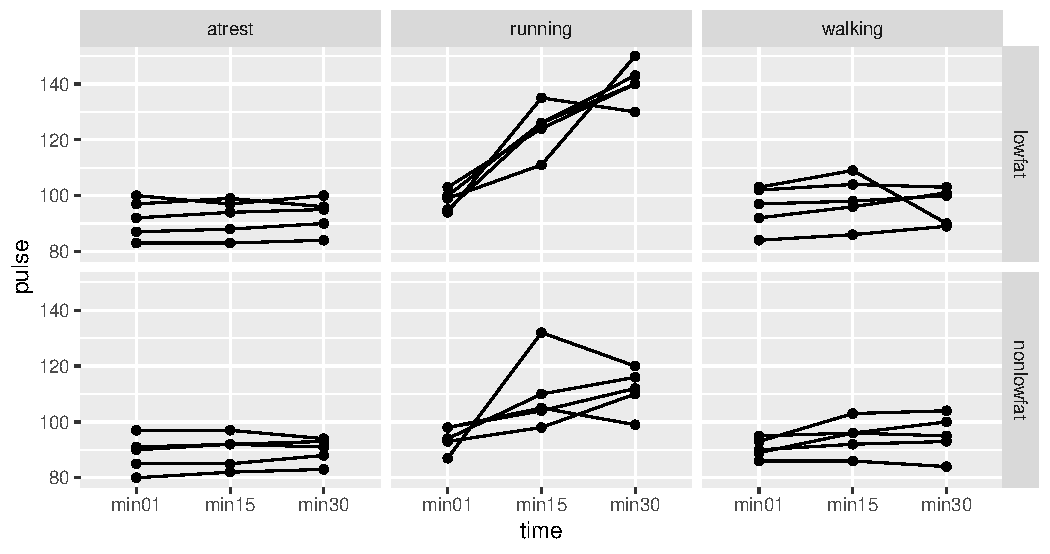
\includegraphics{figure/unnamed-chunk-262-1.pdf}
\caption{plot of chunk unnamed-chunk-262}
\end{figure}

\end{frame}

\begin{frame}[fragile]{Comments on graphs}
\protect\hypertarget{comments-on-graphs}{}

\begin{itemize}
\item
  For subjects who were at rest, no change in pulse rate over time, for
  both diet groups.
\item
  For walking subjects, not much change in pulse rates over time. Maybe
  a small increase on average between 1 and 15 minutes.
\item
  For both running groups, an overall increase in pulse rate over time,
  but the increase is stronger for the \texttt{lowfat} group.
\item
  No consistent effect of diet over all exercise groups.
\item
  No consistent effect of exercise type over both diet groups.
\item
  No consistent effect of time over all diet-exercise type combos.
\end{itemize}

\end{frame}

\begin{frame}[fragile]{``Simple effects'' of diet for the subjects who
ran}
\protect\hypertarget{simple-effects-of-diet-for-the-subjects-who-ran}{}

\begin{itemize}
\item
  Looks as if there is only any substantial time effect for the runners.
  For them, does diet have an effect?
\item
  Pull out only the runners from the wide data:
\end{itemize}

\begin{Shaded}
\begin{Highlighting}[]
\NormalTok{exercise.wide }\OperatorTok
\StringTok{  }\KeywordTok{filter}\NormalTok{(exertype }\OperatorTok{==}\StringTok{ "running"}\NormalTok{) ->}\StringTok{ }\NormalTok{runners.wide}
\end{Highlighting}
\end{Shaded}

\begin{itemize}
\tightlist
\item
  Create response variable and do MANOVA. Some of this looks like
  before, but I have different data now:
\end{itemize}

\footnotesize

\begin{Shaded}
\begin{Highlighting}[]
\NormalTok{response <-}\StringTok{ }\KeywordTok{with}\NormalTok{(runners.wide, }\KeywordTok{cbind}\NormalTok{(min01, min15, min30))}
\NormalTok{runners}\FloatTok{.1}\NormalTok{ <-}\StringTok{ }\KeywordTok{lm}\NormalTok{(response }\OperatorTok{~}\StringTok{ }\NormalTok{diet, }\DataTypeTok{data =}\NormalTok{ runners.wide)}
\NormalTok{times <-}\StringTok{ }\KeywordTok{colnames}\NormalTok{(response)}
\NormalTok{times.df <-}\StringTok{ }\KeywordTok{data.frame}\NormalTok{(times)}
\NormalTok{runners}\FloatTok{.2}\NormalTok{ <-}\StringTok{ }\KeywordTok{Manova}\NormalTok{(runners}\FloatTok{.1}\NormalTok{,}
  \DataTypeTok{idata =}\NormalTok{ times.df,}
  \DataTypeTok{idesign =} \OperatorTok{~}\NormalTok{times}
\NormalTok{)}
\end{Highlighting}
\end{Shaded}

\normalsize

\end{frame}

\begin{frame}[fragile]{Results}
\protect\hypertarget{results-2}{}

\scriptsize

\begin{Shaded}
\begin{Highlighting}[]
\NormalTok{runners}\FloatTok{.2}
\end{Highlighting}
\end{Shaded}

\begin{verbatim}
## 
## Type II Repeated Measures MANOVA Tests: Pillai test statistic
##             Df test stat approx F num Df den Df    Pr(>F)    
## (Intercept)  1   0.99912   9045.3      1      8 1.668e-13 ***
## diet         1   0.84986     45.3      1      8 0.0001482 ***
## times        1   0.92493     43.1      2      7 0.0001159 ***
## diet:times   1   0.68950      7.8      2      7 0.0166807 *  
## ---
## Signif. codes:  0 '***' 0.001 '**' 0.01 '*' 0.05 '.' 0.1 ' ' 1
\end{verbatim}

\normalsize

text under

\begin{itemize}
\item
  The \texttt{diet} by \texttt{time} interaction is still significant
  (at \(\alpha=0.05\)): the effect of time on pulse rates is different
  for the two diets.
\item
  At \(\alpha=0.01\), the interaction is not significant, and then we
  have only two (very) significant main effects of \texttt{diet} and
  \texttt{time}.
\end{itemize}

\end{frame}

\begin{frame}[fragile]{How is the effect of diet different over time?}
\protect\hypertarget{how-is-the-effect-of-diet-different-over-time}{}

\begin{itemize}
\tightlist
\item
  Table of means. Only I need long data for this, so make it (in a
  pipeline):
\end{itemize}

\begin{Shaded}
\begin{Highlighting}[]
\NormalTok{runners.wide }\OperatorTok
\StringTok{  }\KeywordTok{gather}\NormalTok{(time, pulse, min01}\OperatorTok{:}\NormalTok{min30) }\OperatorTok
\StringTok{  }\KeywordTok{group_by}\NormalTok{(time, diet) }\OperatorTok
\StringTok{  }\KeywordTok{summarize}\NormalTok{(}
    \DataTypeTok{mean =} \KeywordTok{mean}\NormalTok{(pulse),}
    \DataTypeTok{sd =} \KeywordTok{sd}\NormalTok{(pulse)}
\NormalTok{  ) ->}\StringTok{ }\NormalTok{summ}
\end{Highlighting}
\end{Shaded}

\begin{itemize}
\tightlist
\item
  Result of \texttt{summarize} is data frame, so can save it (and do
  more with it if needed).
\end{itemize}

\end{frame}

\begin{frame}[fragile]{Understanding diet-time interaction}
\protect\hypertarget{understanding-diet-time-interaction}{}

\begin{itemize}
\tightlist
\item
  The summary:
\end{itemize}

\footnotesize

\begin{Shaded}
\begin{Highlighting}[]
\NormalTok{summ}
\end{Highlighting}
\end{Shaded}

\begin{verbatim}
## # A tibble: 6 x 4
## # Groups:   time [3]
##   time  diet       mean    sd
##   <chr> <chr>     <dbl> <dbl>
## 1 min01 lowfat     98.2  3.70
## 2 min01 nonlowfat  94    4.53
## 3 min15 lowfat    124.   8.62
## 4 min15 nonlowfat 110.  13.1 
## 5 min30 lowfat    141.   7.20
## 6 min30 nonlowfat 111.   7.92
\end{verbatim}

\normalsize

\begin{itemize}
\item
  Pulse rates at any given time higher for \texttt{lowfat} (diet
  effect),
\item
  Pulse rates increase over time of exercise (time effect),
\item
  but the \emph{amount by which pulse rate higher} for a diet depends on
  time: \texttt{diet} by \texttt{time} interaction.
\end{itemize}

\end{frame}

\begin{frame}[fragile]{Interaction plot}
\protect\hypertarget{interaction-plot-4}{}

\begin{itemize}
\tightlist
\item
  We went to trouble of finding means by group, so making interaction
  plot is now mainly easy:
\end{itemize}

\begin{Shaded}
\begin{Highlighting}[]
\KeywordTok{ggplot}\NormalTok{(summ, }\KeywordTok{aes}\NormalTok{(}\DataTypeTok{x =}\NormalTok{ time, }\DataTypeTok{y =}\NormalTok{ mean, }\DataTypeTok{colour =}\NormalTok{ diet,}
                 \DataTypeTok{group =}\NormalTok{ diet)) }\OperatorTok{+}\StringTok{ }\KeywordTok{geom_point}\NormalTok{() }\OperatorTok{+}\StringTok{ }\KeywordTok{geom_line}\NormalTok{()}
\end{Highlighting}
\end{Shaded}

\begin{figure}
\centering
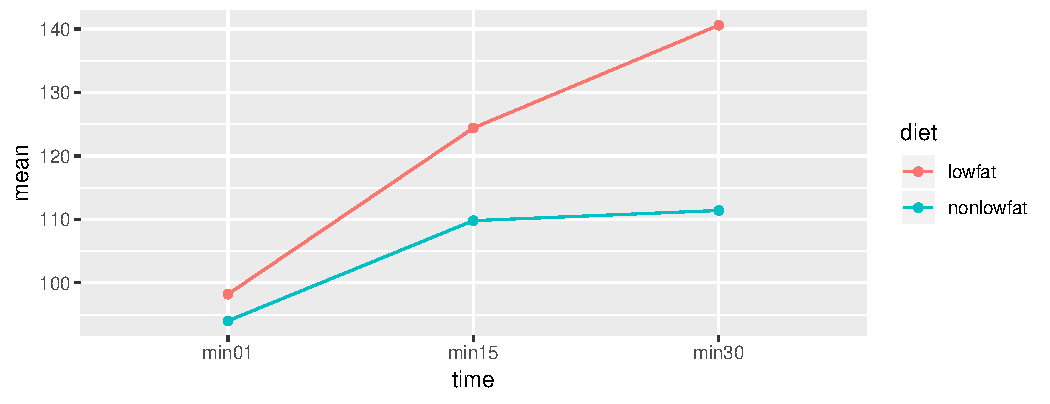
\includegraphics{figure/unnamed-chunk-268-1.pdf}
\caption{plot of chunk unnamed-chunk-268}
\end{figure}

\end{frame}

\begin{frame}{Comment on interaction plot}
\protect\hypertarget{comment-on-interaction-plot}{}

\begin{itemize}
\tightlist
\item
  The lines are not parallel, so there is interaction between diet and
  time for the runners.
\item
  The effect of time on pulse rate is different for the two diets, even
  though all the subjects here were running.
\end{itemize}

\end{frame}

\hypertarget{discriminant-analysis}{%
\section{Discriminant analysis}\label{discriminant-analysis}}

\begin{frame}{Discriminant analysis}
\protect\hypertarget{discriminant-analysis-1}{}

\begin{itemize}
\item
  ANOVA and MANOVA: predict a (counted/measured) response from group
  membership.
\item
  Discriminant analysis: predict group membership based on
  counted/measured variables.
\item
  Covers same ground as logistic regression (and its variations), but
  emphasis on classifying observed data into correct groups.
\item
  Does so by searching for linear combination of original variables that
  best separates data into groups (canonical variables).
\item
  Assumption here that groups are known (for data we have). If trying to
  ``best separate'' data into unknown groups, see \emph{cluster
  analysis}.
\item
  Examples: revisit seed yield and weight data, peanut data,
  professions/activities data; remote-sensing data.
\end{itemize}

\end{frame}

\begin{frame}[fragile]{Packages}
\protect\hypertarget{packages-6}{}

\begin{Shaded}
\begin{Highlighting}[]
\KeywordTok{library}\NormalTok{(MASS)}
\KeywordTok{library}\NormalTok{(tidyverse)}
\KeywordTok{library}\NormalTok{(ggrepel)}
\KeywordTok{library}\NormalTok{(ggbiplot)}
\end{Highlighting}
\end{Shaded}

\texttt{ggrepel} allows labelling points on a plot so they don't
overwrite each other.

\end{frame}

\begin{frame}[fragile]{About \texttt{select}}
\protect\hypertarget{about-select}{}

\begin{itemize}
\item
  Both \texttt{dplyr} (in \texttt{tidyverse}) and \texttt{MASS} have a
  function called \texttt{select}, and \emph{they do
  different things}.
\item
  How do you know which \texttt{select} is going to get called?
\item
  With \texttt{library}, the one loaded \emph{last} is visible, and
  others are not.
\item
  Thus we can access the \texttt{select} in \texttt{dplyr} but not the
  one in \texttt{MASS}. If we wanted that one, we'd have to say
  \texttt{MASS::select}.
\item
  I loaded \texttt{MASS} before \texttt{tidyverse}. If I had done it the
  other way around, the \texttt{tidyverse} \texttt{select}, which I want
  to use, would have been the invisible one.
\item
  Alternative: load \texttt{conflicted} package. Any time you load two
  packages containing functions with same name, you get error and have
  to choose between them.
\end{itemize}

\end{frame}

\begin{frame}[fragile]{Example 1: seed yields and weights}
\protect\hypertarget{example-1-seed-yields-and-weights}{}

\small

\begin{Shaded}
\begin{Highlighting}[]
\NormalTok{my_url <-}\StringTok{ "http://www.utsc.utoronto.ca/~butler/d29/manova1.txt"}
\NormalTok{hilo <-}\StringTok{ }\KeywordTok{read_delim}\NormalTok{(my_url, }\StringTok{" "}\NormalTok{)}
\NormalTok{g <-}\StringTok{ }\KeywordTok{ggplot}\NormalTok{(hilo, }\KeywordTok{aes}\NormalTok{(}
  \DataTypeTok{x =}\NormalTok{ yield, }\DataTypeTok{y =}\NormalTok{ weight,}
  \DataTypeTok{colour =}\NormalTok{ fertilizer}
\NormalTok{)) }\OperatorTok{+}\StringTok{ }\KeywordTok{geom_point}\NormalTok{(}\DataTypeTok{size =} \DecValTok{4}\NormalTok{)}
\end{Highlighting}
\end{Shaded}

\normalsize

\begin{minipage}[t]{0.38\linewidth}
\vspace{0.1\textheight}
Recall data from MANOVA: needed a multivariate analysis to find
difference in seed yield and weight based on whether they were high
or low fertilizer.
\end{minipage}\hfill
\begin{minipage}[t][][b]{0.55\textwidth}
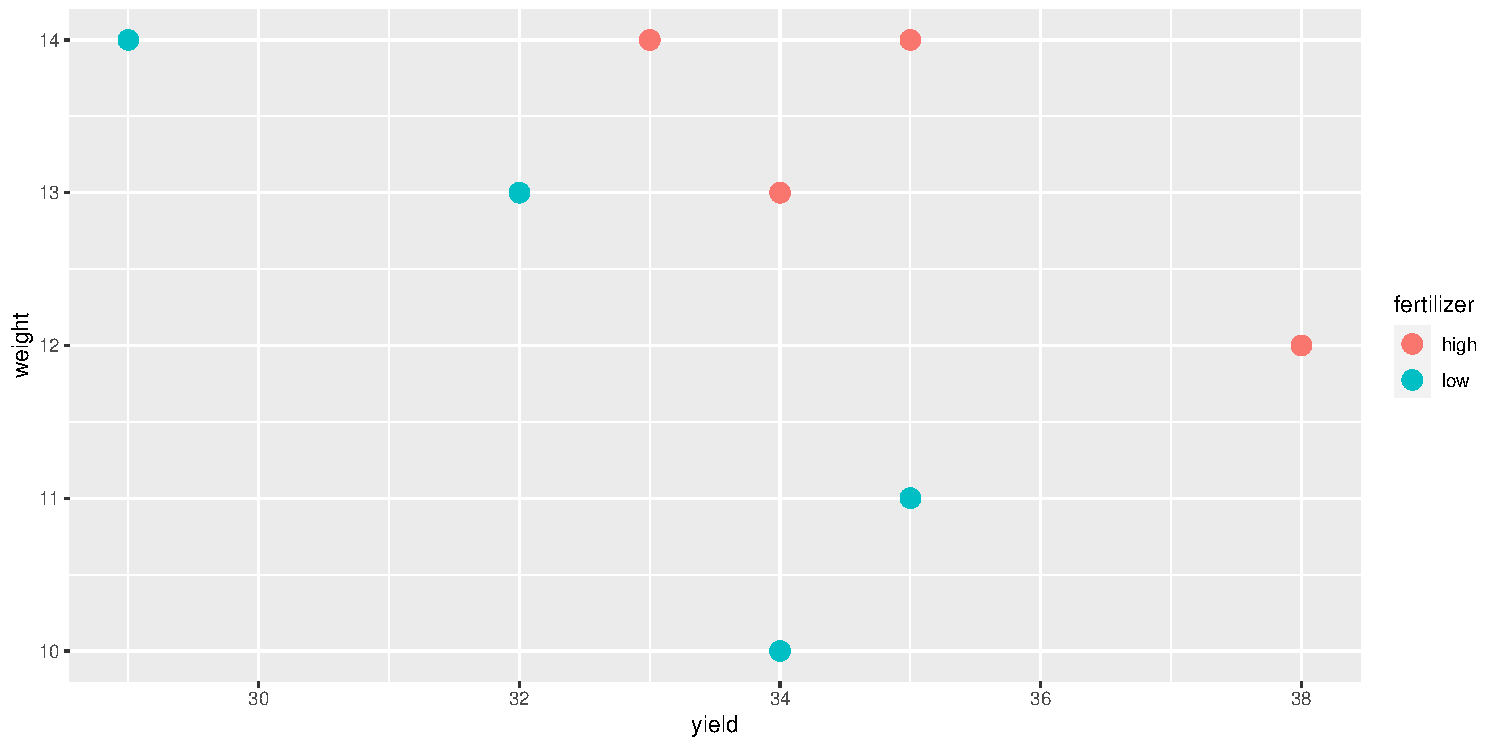
\includegraphics[width=0.9\textwidth, valign=t]{berzani}
\end{minipage}

\end{frame}

\begin{frame}[fragile]{Basic discriminant analysis}
\protect\hypertarget{basic-discriminant-analysis}{}

\begin{Shaded}
\begin{Highlighting}[]
\NormalTok{hilo}\FloatTok{.1}\NormalTok{ <-}\StringTok{ }\KeywordTok{lda}\NormalTok{(fertilizer }\OperatorTok{~}\StringTok{ }\NormalTok{yield }\OperatorTok{+}\StringTok{ }\NormalTok{weight, }\DataTypeTok{data =}\NormalTok{ hilo)}
\end{Highlighting}
\end{Shaded}

\begin{itemize}
\item
  Uses \texttt{lda} from package MASS.
\item
  ``Predicting'' group membership from measured variables.
\end{itemize}

\end{frame}

\begin{frame}[fragile]{Output}
\protect\hypertarget{output-3}{}

\small

\begin{Shaded}
\begin{Highlighting}[]
\NormalTok{hilo}\FloatTok{.1}
\end{Highlighting}
\end{Shaded}

\begin{verbatim}
## Call:
## lda(fertilizer ~ yield + weight, data = hilo)
## 
## Prior probabilities of groups:
## high  low 
##  0.5  0.5 
## 
## Group means:
##      yield weight
## high  35.0  13.25
## low   32.5  12.00
## 
## Coefficients of linear discriminants:
##               LD1
## yield  -0.7666761
## weight -1.2513563
\end{verbatim}

\normalsize

\end{frame}

\begin{frame}{Things to take from output}
\protect\hypertarget{things-to-take-from-output}{}

\begin{itemize}
\item
  Group means: high-fertilizer plants have (slightly) higher mean yield
  and weight than low-fertilizer plants.
\item
  ``Coefficients of linear discriminants'': \texttt{LD1,
  LD2,}\ldots are scores constructed from observed variables that best
  separate the groups.
\item
  For any plant, get LD1 score by taking \(-0.76\) times yield plus
  \(-1.25\) times weight, add up, standardize.
\item
  the LD1 coefficients are like slopes:

  \begin{itemize}
  \tightlist
  \item
    if yield higher, LD1 score for a plant lower
  \item
    if weight higher, LD1 score for a plant lower
  \end{itemize}
\item
  High-fertilizer plants have higher yield and weight, thus low
  (negative) LD1 score. Low-fertilizer plants have low yield and weight,
  thus high (positive) LD1 score.
\item
  One LD1 score for each observation. Plot with actual groups.
\end{itemize}

\end{frame}

\begin{frame}{How many linear discriminants?}
\protect\hypertarget{how-many-linear-discriminants}{}

\begin{itemize}
\item
  Smaller of these:

  \begin{itemize}
  \item
    Number of variables
  \item
    Number of groups \emph{minus 1}
  \end{itemize}
\item
  Seed yield and weight: 2 variables, 2 groups, \(\min(2,2-1)=1\).
\end{itemize}

\end{frame}

\begin{frame}[fragile]{Getting LD scores}
\protect\hypertarget{getting-ld-scores}{}

Feed output from LDA into \texttt{predict}:

\begin{Shaded}
\begin{Highlighting}[]
\NormalTok{hilo.pred <-}\StringTok{ }\KeywordTok{predict}\NormalTok{(hilo}\FloatTok{.1}\NormalTok{)}
\end{Highlighting}
\end{Shaded}

Component \texttt{x} contains LD score(s), here in descending order:

\footnotesize

\begin{Shaded}
\begin{Highlighting}[]
\NormalTok{d <-}\StringTok{ }\KeywordTok{cbind}\NormalTok{(hilo, hilo.pred}\OperatorTok{$}\NormalTok{x) }\OperatorTok\StringTok{ }\KeywordTok{arrange}\NormalTok{(}\KeywordTok{desc}\NormalTok{(LD1))}
\NormalTok{d}
\end{Highlighting}
\end{Shaded}

\begin{verbatim}
##   fertilizer yield weight        LD1
## 1        low    34     10  3.0931414
## 2        low    29     14  1.9210963
## 3        low    35     11  1.0751090
## 4        low    32     13  0.8724245
## 5       high    34     13 -0.6609276
## 6       high    33     14 -1.1456079
## 7       high    38     12 -2.4762756
## 8       high    35     14 -2.6789600
\end{verbatim}

\normalsize

High fertilizer have yield and weight high, negative LD1 scores.

\end{frame}

\begin{frame}[fragile]{Plotting LD1 scores}
\protect\hypertarget{plotting-ld1-scores}{}

With one LD score, plot against (true) groups, eg. boxplot:

\begin{Shaded}
\begin{Highlighting}[]
\KeywordTok{ggplot}\NormalTok{(d, }\KeywordTok{aes}\NormalTok{(}\DataTypeTok{x =}\NormalTok{ fertilizer, }\DataTypeTok{y =}\NormalTok{ LD1)) }\OperatorTok{+}\StringTok{ }\KeywordTok{geom_boxplot}\NormalTok{()}
\end{Highlighting}
\end{Shaded}

\begin{figure}
\centering
\includegraphics{figure/unnamed-chunk-276-1.pdf}
\caption{plot of chunk unnamed-chunk-276}
\end{figure}

\end{frame}

\begin{frame}[fragile]{Potentially misleading}
\protect\hypertarget{potentially-misleading}{}

\begin{Shaded}
\begin{Highlighting}[]
\NormalTok{hilo}\FloatTok{.1}\OperatorTok{$}\NormalTok{scaling}
\end{Highlighting}
\end{Shaded}

\begin{verbatim}
##               LD1
## yield  -0.7666761
## weight -1.2513563
\end{verbatim}

\begin{itemize}
\tightlist
\item
  These are like regression slopes: change in LD1 score for 1-unit
  change in variables.
\end{itemize}

\end{frame}

\begin{frame}[fragile]{But\ldots}
\protect\hypertarget{but-2}{}

\begin{itemize}
\tightlist
\item
  One-unit change in variables might not be comparable:
\end{itemize}

\begin{Shaded}
\begin{Highlighting}[]
\NormalTok{hilo }\OperatorTok\StringTok{ }\KeywordTok{select}\NormalTok{(}\OperatorTok{-}\NormalTok{fertilizer) }\OperatorTok\StringTok{ }
\StringTok{   }\KeywordTok{map_df}\NormalTok{(}\OperatorTok{~}\KeywordTok{quantile}\NormalTok{(., }\KeywordTok{c}\NormalTok{(}\FloatTok{0.25}\NormalTok{, }\FloatTok{0.75}\NormalTok{)))}
\end{Highlighting}
\end{Shaded}

\begin{verbatim}
## # A tibble: 2 x 2
##   yield weight
##   <dbl>  <dbl>
## 1  32.8   11.8
## 2  35     14
\end{verbatim}

\begin{itemize}
\tightlist
\item
  Here, IQRs both 2.2, \emph{identical}, so 1-unit change in each
  variable means same thing.
\end{itemize}

\end{frame}

\begin{frame}[fragile]{What else is in \texttt{hilo.pred?}}
\protect\hypertarget{what-else-is-in-hilo.pred}{}

\small

\begin{Shaded}
\begin{Highlighting}[]
\KeywordTok{names}\NormalTok{(hilo.pred)}
\end{Highlighting}
\end{Shaded}

\begin{verbatim}
## [1] "class"     "posterior" "x"
\end{verbatim}

\normalsize

\begin{itemize}
\item
  \texttt{class}: predicted fertilizer level (based on values of
  \texttt{yield} and \texttt{weight}).
\item
  \texttt{posterior}: predicted probability of being low or high
  fertilizer given \texttt{yield} and \texttt{weight}.
\end{itemize}

\end{frame}

\begin{frame}[fragile]{Predictions and predicted groups}
\protect\hypertarget{predictions-and-predicted-groups}{}

\ldots based on \texttt{yield} and \texttt{weight}:

\footnotesize

\begin{Shaded}
\begin{Highlighting}[]
\KeywordTok{cbind}\NormalTok{(hilo, }\DataTypeTok{predicted =}\NormalTok{ hilo.pred}\OperatorTok{$}\NormalTok{class)}
\end{Highlighting}
\end{Shaded}

\begin{verbatim}
##   fertilizer yield weight predicted
## 1        low    34     10       low
## 2        low    29     14       low
## 3        low    35     11       low
## 4        low    32     13       low
## 5       high    33     14      high
## 6       high    38     12      high
## 7       high    34     13      high
## 8       high    35     14      high
\end{verbatim}

\begin{Shaded}
\begin{Highlighting}[]
\KeywordTok{table}\NormalTok{(}\DataTypeTok{obs =}\NormalTok{ hilo}\OperatorTok{$}\NormalTok{fertilizer, }\DataTypeTok{pred =}\NormalTok{ hilo.pred}\OperatorTok{$}\NormalTok{class)}
\end{Highlighting}
\end{Shaded}

\begin{verbatim}
##       pred
## obs    high low
##   high    4   0
##   low     0   4
\end{verbatim}

\normalsize

\end{frame}

\begin{frame}{Understanding the predicted groups}
\protect\hypertarget{understanding-the-predicted-groups}{}

\begin{itemize}
\item
  Each predicted fertilizer level is exactly same as observed one
  (perfect prediction).
\item
  Table shows no errors: all values on top-left to bottom-right
  diagonal.
\end{itemize}

\end{frame}

\begin{frame}[fragile]{Posterior probabilities}
\protect\hypertarget{posterior-probabilities}{}

show how clear-cut the classification decisions were:

\small

\begin{Shaded}
\begin{Highlighting}[]
\NormalTok{pp <-}\StringTok{ }\KeywordTok{round}\NormalTok{(hilo.pred}\OperatorTok{$}\NormalTok{posterior, }\DecValTok{4}\NormalTok{)}
\NormalTok{d <-}\StringTok{ }\KeywordTok{cbind}\NormalTok{(hilo, hilo.pred}\OperatorTok{$}\NormalTok{x, pp)}
\NormalTok{d}
\end{Highlighting}
\end{Shaded}

\begin{verbatim}
##   fertilizer yield weight        LD1   high    low
## 1        low    34     10  3.0931414 0.0000 1.0000
## 2        low    29     14  1.9210963 0.0012 0.9988
## 3        low    35     11  1.0751090 0.0232 0.9768
## 4        low    32     13  0.8724245 0.0458 0.9542
## 5       high    33     14 -1.1456079 0.9818 0.0182
## 6       high    38     12 -2.4762756 0.9998 0.0002
## 7       high    34     13 -0.6609276 0.9089 0.0911
## 8       high    35     14 -2.6789600 0.9999 0.0001
\end{verbatim}

\normalsize

Only obs.~7 has any doubt: \texttt{yield} low for a high-fertilizer, but
high \texttt{weight} makes up for it.

\end{frame}

\begin{frame}[fragile]{Example 2: the peanuts}
\protect\hypertarget{example-2-the-peanuts}{}

\scriptsize

\begin{Shaded}
\begin{Highlighting}[]
\NormalTok{my_url <-}\StringTok{ "http://www.utsc.utoronto.ca/~butler/d29/peanuts.txt"}
\NormalTok{peanuts <-}\StringTok{ }\KeywordTok{read_delim}\NormalTok{(my_url, }\StringTok{" "}\NormalTok{)}
\NormalTok{peanuts}
\end{Highlighting}
\end{Shaded}

\begin{verbatim}
## # A tibble: 12 x 6
##      obs location variety     y   smk     w
##    <dbl>    <dbl>   <dbl> <dbl> <dbl> <dbl>
##  1     1        1       5  195.  153.  51.4
##  2     2        1       5  194.  168.  53.7
##  3     3        2       5  190.  140.  55.5
##  4     4        2       5  180.  121.  44.4
##  5     5        1       6  203   157.  49.8
##  6     6        1       6  196.  166   45.8
##  7     7        2       6  203.  166.  60.4
##  8     8        2       6  198.  162.  54.1
##  9     9        1       8  194.  164.  57.8
## 10    10        1       8  187   165.  58.6
## 11    11        2       8  202.  167.  65  
## 12    12        2       8  200   174.  67.2
\end{verbatim}

\normalsize

\begin{itemize}
\tightlist
\item
  Recall: \texttt{location} and \texttt{variety} both significant in
  MANOVA. Make combo of them (over):
\end{itemize}

\end{frame}

\begin{frame}[fragile]{Location-variety combos}
\protect\hypertarget{location-variety-combos}{}

\footnotesize

\begin{Shaded}
\begin{Highlighting}[]
\NormalTok{peanuts }\OperatorTok
\StringTok{   }\KeywordTok{unite}\NormalTok{(combo, }\KeywordTok{c}\NormalTok{(variety, location)) ->}\StringTok{ }\NormalTok{peanuts.combo}
\NormalTok{peanuts.combo}
\end{Highlighting}
\end{Shaded}

\begin{verbatim}
## # A tibble: 12 x 5
##      obs combo     y   smk     w
##    <dbl> <chr> <dbl> <dbl> <dbl>
##  1     1 5_1    195.  153.  51.4
##  2     2 5_1    194.  168.  53.7
##  3     3 5_2    190.  140.  55.5
##  4     4 5_2    180.  121.  44.4
##  5     5 6_1    203   157.  49.8
##  6     6 6_1    196.  166   45.8
##  7     7 6_2    203.  166.  60.4
##  8     8 6_2    198.  162.  54.1
##  9     9 8_1    194.  164.  57.8
## 10    10 8_1    187   165.  58.6
## 11    11 8_2    202.  167.  65  
## 12    12 8_2    200   174.  67.2
\end{verbatim}

\normalsize

\end{frame}

\begin{frame}[fragile]{Discriminant analysis}
\protect\hypertarget{discriminant-analysis-2}{}

\small

\begin{Shaded}
\begin{Highlighting}[]
\NormalTok{peanuts}\FloatTok{.1}\NormalTok{ <-}\StringTok{ }\KeywordTok{lda}\NormalTok{(combo }\OperatorTok{~}\StringTok{ }\NormalTok{y }\OperatorTok{+}\StringTok{ }\NormalTok{smk }\OperatorTok{+}\StringTok{ }\NormalTok{w, }\DataTypeTok{data =}\NormalTok{ peanuts.combo)}
\NormalTok{peanuts}\FloatTok{.1}\OperatorTok{$}\NormalTok{scaling}
\end{Highlighting}
\end{Shaded}

\begin{verbatim}
##            LD1         LD2         LD3
## y   -0.4027356 -0.02967881  0.18839237
## smk -0.1727459  0.06794271 -0.09386294
## w    0.5792456  0.16300221  0.07341123
\end{verbatim}

\begin{Shaded}
\begin{Highlighting}[]
\NormalTok{peanuts}\FloatTok{.1}\OperatorTok{$}\NormalTok{svd}
\end{Highlighting}
\end{Shaded}

\begin{verbatim}
## [1] 6.141323 2.428396 1.075589
\end{verbatim}

\normalsize

\begin{itemize}
\tightlist
\item
  Now 3 LDs (3 variables, 6 groups, \(\min(3,6-1)=3\)).
\end{itemize}

\end{frame}

\begin{frame}[fragile]{Comments}
\protect\hypertarget{comments-22}{}

\begin{itemize}
\item
  First: relationship of LDs to original variables. Look for coeffs far
  from zero: here,

  \begin{itemize}
  \item
    high \texttt{LD1} mainly high \texttt{w} or low \texttt{y}.
  \item
    high \texttt{LD2} mainly high \texttt{w}.
  \end{itemize}
\item
  \texttt{svd} values show relative importance of LDs: \texttt{LD1} much
  more important than \texttt{LD2}.
\end{itemize}

\end{frame}

\begin{frame}[fragile]{Group means by variable}
\protect\hypertarget{group-means-by-variable}{}

\begin{Shaded}
\begin{Highlighting}[]
\NormalTok{peanuts}\FloatTok{.1}\OperatorTok{$}\NormalTok{means}
\end{Highlighting}
\end{Shaded}

\begin{verbatim}
##          y    smk     w
## 5_1 194.80 160.40 52.55
## 5_2 185.05 130.30 49.95
## 6_1 199.45 161.40 47.80
## 6_2 200.15 163.95 57.25
## 8_1 190.25 164.80 58.20
## 8_2 200.75 170.30 66.10
\end{verbatim}

\begin{itemize}
\item
  \texttt{5\_2} clearly smallest on \texttt{y}, \texttt{smk}, near
  smallest on \texttt{w}
\item
  \texttt{8\_2} clearly biggest on \texttt{smk}, \texttt{w}, also
  largest on \texttt{y}
\item
  \texttt{8\_1} large on \texttt{w}, small on \texttt{y}.
\end{itemize}

\end{frame}

\begin{frame}[fragile]{The predictions and misclassification}
\protect\hypertarget{the-predictions-and-misclassification}{}

\begin{Shaded}
\begin{Highlighting}[]
\NormalTok{peanuts.pred <-}\StringTok{ }\KeywordTok{predict}\NormalTok{(peanuts}\FloatTok{.1}\NormalTok{)}
\KeywordTok{table}\NormalTok{(}
  \DataTypeTok{obs =}\NormalTok{ peanuts.combo}\OperatorTok{$}\NormalTok{combo,}
  \DataTypeTok{pred =}\NormalTok{ peanuts.pred}\OperatorTok{$}\NormalTok{class}
\NormalTok{)}
\end{Highlighting}
\end{Shaded}

\begin{verbatim}
##      pred
## obs   5_1 5_2 6_1 6_2 8_1 8_2
##   5_1   2   0   0   0   0   0
##   5_2   0   2   0   0   0   0
##   6_1   0   0   2   0   0   0
##   6_2   1   0   0   1   0   0
##   8_1   0   0   0   0   2   0
##   8_2   0   0   0   0   0   2
\end{verbatim}

Actually classified very well. Only one \texttt{6\_2} classified as a
\texttt{5\_1}, rest all correct.

\end{frame}

\begin{frame}[fragile]{Posterior probabilities}
\protect\hypertarget{posterior-probabilities-1}{}

\scriptsize

\begin{Shaded}
\begin{Highlighting}[]
\NormalTok{pp <-}\StringTok{ }\KeywordTok{round}\NormalTok{(peanuts.pred}\OperatorTok{$}\NormalTok{posterior, }\DecValTok{2}\NormalTok{)}
\NormalTok{peanuts.combo }\OperatorTok
\StringTok{  }\KeywordTok{select}\NormalTok{(}\OperatorTok{-}\KeywordTok{c}\NormalTok{(y, smk, w)) }\OperatorTok
\StringTok{  }\KeywordTok{cbind}\NormalTok{(., }\DataTypeTok{pred =}\NormalTok{ peanuts.pred}\OperatorTok{$}\NormalTok{class, pp)}
\end{Highlighting}
\end{Shaded}

\begin{verbatim}
##    obs combo pred  5_1 5_2 6_1  6_2  8_1  8_2
## 1    1   5_1  5_1 0.69   0   0 0.31 0.00 0.00
## 2    2   5_1  5_1 0.73   0   0 0.27 0.00 0.00
## 3    3   5_2  5_2 0.00   1   0 0.00 0.00 0.00
## 4    4   5_2  5_2 0.00   1   0 0.00 0.00 0.00
## 5    5   6_1  6_1 0.00   0   1 0.00 0.00 0.00
## 6    6   6_1  6_1 0.00   0   1 0.00 0.00 0.00
## 7    7   6_2  6_2 0.13   0   0 0.87 0.00 0.00
## 8    8   6_2  5_1 0.53   0   0 0.47 0.00 0.00
## 9    9   8_1  8_1 0.02   0   0 0.02 0.75 0.21
## 10  10   8_1  8_1 0.00   0   0 0.00 0.99 0.01
## 11  11   8_2  8_2 0.00   0   0 0.00 0.03 0.97
## 12  12   8_2  8_2 0.00   0   0 0.00 0.06 0.94
\end{verbatim}

\normalsize

\emph{Some} doubt about which combo each plant belongs in, but not too
much. The one misclassified plant was a close call.

\end{frame}

\begin{frame}[fragile]{Discriminant scores, again}
\protect\hypertarget{discriminant-scores-again}{}

\begin{itemize}
\item
  How are discriminant scores related to original variables?
\item
  Construct data frame with original data and discriminant scores side
  by side:
\end{itemize}

\footnotesize

\begin{Shaded}
\begin{Highlighting}[]
\NormalTok{peanuts}\FloatTok{.1}\OperatorTok{$}\NormalTok{scaling}
\end{Highlighting}
\end{Shaded}

\begin{verbatim}
##            LD1         LD2         LD3
## y   -0.4027356 -0.02967881  0.18839237
## smk -0.1727459  0.06794271 -0.09386294
## w    0.5792456  0.16300221  0.07341123
\end{verbatim}

\begin{Shaded}
\begin{Highlighting}[]
\NormalTok{lds <-}\StringTok{ }\KeywordTok{round}\NormalTok{(peanuts.pred}\OperatorTok{$}\NormalTok{x, }\DecValTok{2}\NormalTok{)}
\NormalTok{mm <-}\StringTok{ }\KeywordTok{with}\NormalTok{(peanuts.combo,}
           \KeywordTok{data.frame}\NormalTok{(combo, y, smk, w, lds))}
\end{Highlighting}
\end{Shaded}

\normalsize

\begin{itemize}
\item
  LD1 positive if \texttt{w} large and/or \texttt{y} small.
\item
  LD2 positive if \texttt{w} large.
\end{itemize}

\end{frame}

\begin{frame}[fragile]{Discriminant scores for data}
\protect\hypertarget{discriminant-scores-for-data}{}

\footnotesize

\begin{Shaded}
\begin{Highlighting}[]
\NormalTok{mm}
\end{Highlighting}
\end{Shaded}

\begin{verbatim}
##    combo     y   smk    w   LD1   LD2   LD3
## 1    5_1 195.3 153.1 51.4 -1.42 -1.01  0.26
## 2    5_1 194.3 167.7 53.7 -2.20  0.38 -1.13
## 3    5_2 189.7 139.5 55.5  5.56 -1.10  0.79
## 4    5_2 180.4 121.1 44.4  6.06 -3.89 -0.05
## 5    6_1 203.0 156.8 49.8 -6.08 -1.25  1.25
## 6    6_1 195.9 166.0 45.8 -7.13 -1.07 -1.24
## 7    6_2 202.7 166.1 60.4 -1.43  1.12  1.10
## 8    6_2 197.6 161.8 54.1 -2.28 -0.05  0.08
## 9    8_1 193.5 164.5 57.8  1.05  0.86 -0.67
## 10   8_1 187.0 165.1 58.6  4.02  1.22 -1.90
## 11   8_2 201.5 166.8 65.0  1.60  1.95  1.15
## 12   8_2 200.0 173.8 67.2  2.27  2.83  0.37
\end{verbatim}

\normalsize

\begin{itemize}
\item
  Obs.~5 and 6 have most negative \texttt{LD1}: large \texttt{y}, small
  \texttt{w}.
\item
  Obs.~4 has most negative \texttt{LD2}: small \texttt{w}.
\end{itemize}

\end{frame}

\begin{frame}[fragile]{Predict typical LD1 scores}
\protect\hypertarget{predict-typical-ld1-scores}{}

First and third quartiles for three response variables:

\begin{Shaded}
\begin{Highlighting}[]
\NormalTok{quartiles <-}\StringTok{ }\NormalTok{peanuts }\OperatorTok
\StringTok{  }\KeywordTok{select}\NormalTok{(y}\OperatorTok{:}\NormalTok{w) }\OperatorTok
\StringTok{  }\KeywordTok{map_df}\NormalTok{(quantile, }\KeywordTok{c}\NormalTok{(}\FloatTok{0.25}\NormalTok{, }\FloatTok{0.75}\NormalTok{))}
\NormalTok{quartiles}
\end{Highlighting}
\end{Shaded}

\begin{verbatim}
## # A tibble: 2 x 3
##       y   smk     w
##   <dbl> <dbl> <dbl>
## 1  193.  156.  51  
## 2  200.  166.  59.0
\end{verbatim}

\begin{Shaded}
\begin{Highlighting}[]
\NormalTok{new <-}\StringTok{ }\KeywordTok{with}\NormalTok{(quartiles, }\KeywordTok{crossing}\NormalTok{(y, smk, w))}
\end{Highlighting}
\end{Shaded}

\end{frame}

\begin{frame}[fragile]{The combinations}
\protect\hypertarget{the-combinations}{}

\begin{Shaded}
\begin{Highlighting}[]
\NormalTok{new}
\end{Highlighting}
\end{Shaded}

\begin{verbatim}
## # A tibble: 8 x 3
##       y   smk     w
##   <dbl> <dbl> <dbl>
## 1  193.  156.  51  
## 2  193.  156.  59.0
## 3  193.  166.  51  
## 4  193.  166.  59.0
## 5  200.  156.  51  
## 6  200.  156.  59.0
## 7  200.  166.  51  
## 8  200.  166.  59.0
\end{verbatim}

\begin{Shaded}
\begin{Highlighting}[]
\NormalTok{pp <-}\StringTok{ }\KeywordTok{predict}\NormalTok{(peanuts}\FloatTok{.1}\NormalTok{, new)}
\end{Highlighting}
\end{Shaded}

\end{frame}

\begin{frame}[fragile]{Predicted typical LD1 scores}
\protect\hypertarget{predicted-typical-ld1-scores}{}

\footnotesize

\begin{Shaded}
\begin{Highlighting}[]
\KeywordTok{cbind}\NormalTok{(new, pp}\OperatorTok{$}\NormalTok{x) }\OperatorTok\StringTok{ }\KeywordTok{arrange}\NormalTok{(LD1)}
\end{Highlighting}
\end{Shaded}

\begin{verbatim}
##         y     smk     w        LD1        LD2         LD3
## 1 200.375 166.275 51.00 -5.9688625 -0.3330095 -0.04523828
## 2 200.375 155.875 51.00 -4.1723048 -1.0396138  0.93093630
## 3 192.550 166.275 51.00 -2.8174566 -0.1007728 -1.51940856
## 4 200.375 166.275 59.05 -1.3059358  0.9791583  0.54572212
## 5 192.550 155.875 51.00 -1.0208989 -0.8073770 -0.54323399
## 6 200.375 155.875 59.05  0.4906219  0.2725540  1.52189670
## 7 192.550 166.275 59.05  1.8454701  1.2113950 -0.92844817
## 8 192.550 155.875 59.05  3.6420278  0.5047907  0.04772641
\end{verbatim}

\normalsize

\begin{itemize}
\item
  Very negative LD1 score with large \texttt{y} and small \texttt{w}
\item
  \texttt{smk} doesn't contribute much to LD1
\item
  Very positive LD1 score with small \texttt{y} and large \texttt{w}.
\item
  Same as we saw from Coefficients of Linear Discriminants.
\end{itemize}

\end{frame}

\begin{frame}[fragile]{Plot LD1 vs.~LD2, labelling by combo}
\protect\hypertarget{plot-ld1-vs.ld2-labelling-by-combo}{}

\begin{Shaded}
\begin{Highlighting}[]
\NormalTok{g <-}\StringTok{ }\KeywordTok{ggplot}\NormalTok{(mm, }\KeywordTok{aes}\NormalTok{(}\DataTypeTok{x =}\NormalTok{ LD1, }\DataTypeTok{y =}\NormalTok{ LD2, }\DataTypeTok{colour =}\NormalTok{ combo, }
                    \DataTypeTok{label =}\NormalTok{ combo)) }\OperatorTok{+}\StringTok{ }\KeywordTok{geom_point}\NormalTok{() }\OperatorTok{+}
\StringTok{  }\KeywordTok{geom_text_repel}\NormalTok{() }\OperatorTok{+}\StringTok{ }\KeywordTok{guides}\NormalTok{(}\DataTypeTok{colour =}\NormalTok{ F)}
\NormalTok{g}
\end{Highlighting}
\end{Shaded}

\begin{figure}
\centering
\includegraphics{figure/unnamed-chunk-292-1.pdf}
\caption{plot of chunk unnamed-chunk-292}
\end{figure}

\end{frame}

\begin{frame}[fragile]{``Bi-plot'' from \texttt{ggbiplot}}
\protect\hypertarget{bi-plot-from-ggbiplot}{}

\begin{Shaded}
\begin{Highlighting}[]
\KeywordTok{ggbiplot}\NormalTok{(peanuts}\FloatTok{.1}\NormalTok{,}
  \DataTypeTok{groups =} \KeywordTok{factor}\NormalTok{(peanuts.combo}\OperatorTok{$}\NormalTok{combo)}
\NormalTok{)}
\end{Highlighting}
\end{Shaded}

\begin{figure}
\centering
\includegraphics{figure/unnamed-chunk-293-1.pdf}
\caption{plot of chunk unnamed-chunk-293}
\end{figure}

\end{frame}

\begin{frame}[fragile]{Installing \texttt{ggbiplot}}
\protect\hypertarget{installing-ggbiplot}{}

\begin{itemize}
\item
  \texttt{ggbiplot} not on CRAN, so usual \texttt{install.packages} will
  not work.
\item
  Install package \texttt{devtools} first (once):
\end{itemize}

\begin{Shaded}
\begin{Highlighting}[]
\KeywordTok{install.packages}\NormalTok{(}\StringTok{"devtools"}\NormalTok{)}
\end{Highlighting}
\end{Shaded}

\begin{itemize}
\tightlist
\item
  Then install \texttt{ggbiplot} (once):
\end{itemize}

\begin{Shaded}
\begin{Highlighting}[]
\KeywordTok{library}\NormalTok{(devtools)}
\KeywordTok{install_github}\NormalTok{(}\StringTok{"vqv/ggbiplot"}\NormalTok{)}
\end{Highlighting}
\end{Shaded}

\end{frame}

\begin{frame}{Cross-validation}
\protect\hypertarget{cross-validation}{}

\begin{itemize}
\item
  So far, have predicted group membership from same data used to form
  the groups --- dishonest!
\item
  Better: \emph{cross-validation}: form groups from all observations
  \emph{except one}, then predict group membership for that left-out
  observation.
\item
  No longer cheating!
\item
  Illustrate with peanuts data again.
\end{itemize}

\end{frame}

\begin{frame}[fragile]{Misclassifications}
\protect\hypertarget{misclassifications}{}

\begin{itemize}
\tightlist
\item
  Fitting and prediction all in one go:
\end{itemize}

\small

\begin{Shaded}
\begin{Highlighting}[]
\NormalTok{peanuts.cv <-}\StringTok{ }\KeywordTok{lda}\NormalTok{(combo }\OperatorTok{~}\StringTok{ }\NormalTok{y }\OperatorTok{+}\StringTok{ }\NormalTok{smk }\OperatorTok{+}\StringTok{ }\NormalTok{w,}
  \DataTypeTok{data =}\NormalTok{ peanuts.combo, }\DataTypeTok{CV =}\NormalTok{ T)}
\KeywordTok{table}\NormalTok{(}\DataTypeTok{obs =}\NormalTok{ peanuts.combo}\OperatorTok{$}\NormalTok{combo,}
      \DataTypeTok{pred =}\NormalTok{ peanuts.cv}\OperatorTok{$}\NormalTok{class)}
\end{Highlighting}
\end{Shaded}

\begin{verbatim}
##      pred
## obs   5_1 5_2 6_1 6_2 8_1 8_2
##   5_1   0   0   0   2   0   0
##   5_2   0   1   0   0   1   0
##   6_1   0   0   2   0   0   0
##   6_2   1   0   0   1   0   0
##   8_1   0   1   0   0   0   1
##   8_2   0   0   0   0   0   2
\end{verbatim}

\normalsize

\begin{itemize}
\tightlist
\item
  Some more misclassification this time.
\end{itemize}

\end{frame}

\begin{frame}[fragile]{Repeat of LD plot}
\protect\hypertarget{repeat-of-ld-plot}{}

\begin{Shaded}
\begin{Highlighting}[]
\NormalTok{g}
\end{Highlighting}
\end{Shaded}

\begin{figure}
\centering
\includegraphics{figure/graziani-1.pdf}
\caption{plot of chunk graziani}
\end{figure}

\end{frame}

\begin{frame}[fragile]{Posterior probabilities}
\protect\hypertarget{posterior-probabilities-2}{}

\footnotesize

\begin{Shaded}
\begin{Highlighting}[]
\NormalTok{pp <-}\StringTok{ }\KeywordTok{round}\NormalTok{(peanuts.cv}\OperatorTok{$}\NormalTok{posterior, }\DecValTok{3}\NormalTok{)}
\KeywordTok{data.frame}\NormalTok{(}
  \DataTypeTok{obs =}\NormalTok{ peanuts.combo}\OperatorTok{$}\NormalTok{combo,}
  \DataTypeTok{pred =}\NormalTok{ peanuts.cv}\OperatorTok{$}\NormalTok{class, pp}
\NormalTok{)}
\end{Highlighting}
\end{Shaded}

\begin{verbatim}
##    obs pred  X5_1 X5_2  X6_1  X6_2  X8_1  X8_2
## 1  5_1  6_2 0.162 0.00 0.000 0.838 0.000 0.000
## 2  5_1  6_2 0.200 0.00 0.000 0.799 0.000 0.000
## 3  5_2  8_1 0.000 0.18 0.000 0.000 0.820 0.000
## 4  5_2  5_2 0.000 1.00 0.000 0.000 0.000 0.000
## 5  6_1  6_1 0.194 0.00 0.669 0.137 0.000 0.000
## 6  6_1  6_1 0.000 0.00 1.000 0.000 0.000 0.000
## 7  6_2  6_2 0.325 0.00 0.000 0.667 0.001 0.008
## 8  6_2  5_1 0.821 0.00 0.000 0.179 0.000 0.000
## 9  8_1  8_2 0.000 0.00 0.000 0.000 0.000 1.000
## 10 8_1  5_2 0.000 1.00 0.000 0.000 0.000 0.000
## 11 8_2  8_2 0.001 0.00 0.000 0.004 0.083 0.913
## 12 8_2  8_2 0.000 0.00 0.000 0.000 0.167 0.833
\end{verbatim}

\normalsize

\end{frame}

\begin{frame}[fragile]{Why more misclassification?}
\protect\hypertarget{why-more-misclassification}{}

\begin{itemize}
\item
  When predicting group membership for one observation, only uses the
  \emph{other one} in that group.
\item
  So if two in a pair are far apart, or if two groups overlap, great
  potential for misclassification.
\item
  Groups \texttt{5\_1} and \texttt{6\_2} overlap.
\item
  \texttt{5\_2} closest to \texttt{8\_1}s looks more like an
  \texttt{8\_1} than a \texttt{5\_2} (other one far away).
\item
  \texttt{8\_1}s relatively far apart and close to other things, so one
  appears to be a \texttt{5\_2} and the other an \texttt{8\_2}.
\end{itemize}

\end{frame}

\begin{frame}[fragile]{Example 3: professions and leisure activities}
\protect\hypertarget{example-3-professions-and-leisure-activities}{}

\begin{itemize}
\item
  15 individuals from three different professions (politicians,
  administrators and belly dancers) each participate in four different
  leisure activities: reading, dancing, TV watching and skiing. After
  each activity they rate it on a 0--10 scale.
\item
  Some of the data:
\end{itemize}

\normalsize

\begin{verbatim}
bellydancer 7 10 6 5
bellydancer 8 9 5 7
bellydancer 5 10 5 8
politician 5 5 5 6
politician 4 5 6 5
admin 4 2 2 5
admin 7 1 2 4
admin 6 3 3 3
\end{verbatim}

\normalsize

\end{frame}

\begin{frame}{Questions}
\protect\hypertarget{questions}{}

\begin{itemize}
\item
  How can we best use the scores on the activities to predict a person's
  profession?
\item
  Or, what combination(s) of scores best separate data into profession
  groups?
\end{itemize}

\end{frame}

\begin{frame}[fragile]{Discriminant analysis}
\protect\hypertarget{discriminant-analysis-3}{}

\small

\begin{Shaded}
\begin{Highlighting}[]
\NormalTok{my_url <-}\StringTok{ "http://www.utsc.utoronto.ca/~butler/d29/profile.txt"}
\NormalTok{active <-}\StringTok{ }\KeywordTok{read_delim}\NormalTok{(my_url, }\StringTok{" "}\NormalTok{)}
\NormalTok{active}\FloatTok{.1}\NormalTok{ <-}\StringTok{ }\KeywordTok{lda}\NormalTok{(job }\OperatorTok{~}\StringTok{ }\NormalTok{reading }\OperatorTok{+}\StringTok{ }\NormalTok{dance }\OperatorTok{+}\StringTok{ }\NormalTok{tv }\OperatorTok{+}\StringTok{ }\NormalTok{ski, }\DataTypeTok{data =}\NormalTok{ active)}
\NormalTok{active}\FloatTok{.1}\OperatorTok{$}\NormalTok{svd}
\end{Highlighting}
\end{Shaded}

\begin{verbatim}
## [1] 9.856638 3.434555
\end{verbatim}

\begin{Shaded}
\begin{Highlighting}[]
\NormalTok{active}\FloatTok{.1}\OperatorTok{$}\NormalTok{scaling}
\end{Highlighting}
\end{Shaded}

\begin{verbatim}
##                 LD1        LD2
## reading -0.01297465  0.4748081
## dance   -0.95212396  0.4614976
## tv      -0.47417264 -1.2446327
## ski      0.04153684  0.2033122
\end{verbatim}

\normalsize

\begin{itemize}
\item
  Two discriminants, first fair bit more important than second.
\item
  \texttt{LD1} depends (negatively) most on \texttt{dance}, a bit on
  \texttt{tv}.
\item
  \texttt{LD2} depends mostly on \texttt{tv}.
\end{itemize}

\end{frame}

\begin{frame}[fragile]{Misclassification}
\protect\hypertarget{misclassification}{}

\begin{Shaded}
\begin{Highlighting}[]
\NormalTok{active.pred <-}\StringTok{ }\KeywordTok{predict}\NormalTok{(active}\FloatTok{.1}\NormalTok{)}
\KeywordTok{table}\NormalTok{(}\DataTypeTok{obs =}\NormalTok{ active}\OperatorTok{$}\NormalTok{job, }\DataTypeTok{pred =}\NormalTok{ active.pred}\OperatorTok{$}\NormalTok{class)}
\end{Highlighting}
\end{Shaded}

\begin{verbatim}
##              pred
## obs           admin bellydancer politician
##   admin           5           0          0
##   bellydancer     0           5          0
##   politician      0           0          5
\end{verbatim}

Everyone correctly classified.

\end{frame}

\begin{frame}[fragile]{Plotting LDs}
\protect\hypertarget{plotting-lds}{}

\small

\begin{Shaded}
\begin{Highlighting}[]
\NormalTok{mm <-}\StringTok{ }\KeywordTok{data.frame}\NormalTok{(}\DataTypeTok{job =}\NormalTok{ active}\OperatorTok{$}\NormalTok{job, active.pred}\OperatorTok{$}\NormalTok{x, }\DataTypeTok{person =} \DecValTok{1}\OperatorTok{:}\DecValTok{15}\NormalTok{)}
\NormalTok{g <-}\StringTok{ }\KeywordTok{ggplot}\NormalTok{(mm, }\KeywordTok{aes}\NormalTok{(}\DataTypeTok{x =}\NormalTok{ LD1, }\DataTypeTok{y =}\NormalTok{ LD2, }\DataTypeTok{colour =}\NormalTok{ job, }
                    \DataTypeTok{label =}\NormalTok{ job)) }\OperatorTok{+}\StringTok{ }
\StringTok{  }\KeywordTok{geom_point}\NormalTok{() }\OperatorTok{+}\StringTok{ }\KeywordTok{geom_text_repel}\NormalTok{() }\OperatorTok{+}\StringTok{ }\KeywordTok{guides}\NormalTok{(}\DataTypeTok{colour =}\NormalTok{ F)}
\NormalTok{g}
\end{Highlighting}
\end{Shaded}

\includegraphics{figure/unnamed-chunk-300-1.pdf} \normalsize

\end{frame}

\begin{frame}[fragile]{Biplot}
\protect\hypertarget{biplot}{}

\begin{Shaded}
\begin{Highlighting}[]
\KeywordTok{ggbiplot}\NormalTok{(active}\FloatTok{.1}\NormalTok{, }\DataTypeTok{groups =}\NormalTok{ active}\OperatorTok{$}\NormalTok{job)}
\end{Highlighting}
\end{Shaded}

\begin{figure}
\centering
\includegraphics{figure/unnamed-chunk-301-1.pdf}
\caption{plot of chunk unnamed-chunk-301}
\end{figure}

\end{frame}

\begin{frame}[fragile]{Comments on plot}
\protect\hypertarget{comments-on-plot}{}

\begin{itemize}
\item
  Groups well separated: bellydancers top left, administrators top
  right, politicians lower middle.
\item
  Bellydancers most negative on \texttt{LD1}: like dancing most.
\item
  Administrators most positive on \texttt{LD1}: like dancing least.
\item
  Politicians most negative on \texttt{LD2}: like TV-watching most.
\end{itemize}

\end{frame}

\begin{frame}[fragile]{Plotting individual \texttt{persons}}
\protect\hypertarget{plotting-individual-persons}{}

Make \texttt{label} be identifier of person. Now need legend:

\begin{Shaded}
\begin{Highlighting}[]
\KeywordTok{ggplot}\NormalTok{(mm, }\KeywordTok{aes}\NormalTok{(}\DataTypeTok{x =}\NormalTok{ LD1, }\DataTypeTok{y =}\NormalTok{ LD2,  }\DataTypeTok{colour =}\NormalTok{ job, }
               \DataTypeTok{label =}\NormalTok{ person)) }\OperatorTok{+}\StringTok{ }
\StringTok{  }\KeywordTok{geom_point}\NormalTok{() }\OperatorTok{+}\StringTok{ }\KeywordTok{geom_text_repel}\NormalTok{()}
\end{Highlighting}
\end{Shaded}

\begin{figure}
\centering
\includegraphics{figure/unnamed-chunk-302-1.pdf}
\caption{plot of chunk unnamed-chunk-302}
\end{figure}

\end{frame}

\begin{frame}[fragile]{Posterior probabilities}
\protect\hypertarget{posterior-probabilities-3}{}

\scriptsize

\begin{Shaded}
\begin{Highlighting}[]
\NormalTok{pp <-}\StringTok{ }\KeywordTok{round}\NormalTok{(active.pred}\OperatorTok{$}\NormalTok{posterior, }\DecValTok{3}\NormalTok{)}
\KeywordTok{data.frame}\NormalTok{(}\DataTypeTok{obs =}\NormalTok{ active}\OperatorTok{$}\NormalTok{job, }\DataTypeTok{pred =}\NormalTok{ active.pred}\OperatorTok{$}\NormalTok{class, pp)}
\end{Highlighting}
\end{Shaded}

\begin{verbatim}
##            obs        pred admin bellydancer politician
## 1  bellydancer bellydancer 0.000       1.000      0.000
## 2  bellydancer bellydancer 0.000       1.000      0.000
## 3  bellydancer bellydancer 0.000       1.000      0.000
## 4  bellydancer bellydancer 0.000       1.000      0.000
## 5  bellydancer bellydancer 0.000       0.997      0.003
## 6   politician  politician 0.003       0.000      0.997
## 7   politician  politician 0.000       0.000      1.000
## 8   politician  politician 0.000       0.000      1.000
## 9   politician  politician 0.000       0.002      0.998
## 10  politician  politician 0.000       0.000      1.000
## 11       admin       admin 1.000       0.000      0.000
## 12       admin       admin 1.000       0.000      0.000
## 13       admin       admin 1.000       0.000      0.000
## 14       admin       admin 1.000       0.000      0.000
## 15       admin       admin 0.982       0.000      0.018
\end{verbatim}

\normalsize

Not much doubt.

\end{frame}

\begin{frame}[fragile]{Cross-validating the jobs-activities data}
\protect\hypertarget{cross-validating-the-jobs-activities-data}{}

Recall: no need for \texttt{predict}. Just pull out \texttt{class} and
make a table:

\begin{Shaded}
\begin{Highlighting}[]
\NormalTok{active.cv <-}\StringTok{ }\KeywordTok{lda}\NormalTok{(job }\OperatorTok{~}\StringTok{ }\NormalTok{reading }\OperatorTok{+}\StringTok{ }\NormalTok{dance }\OperatorTok{+}\StringTok{ }\NormalTok{tv }\OperatorTok{+}\StringTok{ }\NormalTok{ski,}
  \DataTypeTok{data =}\NormalTok{ active, }\DataTypeTok{CV =}\NormalTok{ T}
\NormalTok{)}
\KeywordTok{table}\NormalTok{(}\DataTypeTok{obs =}\NormalTok{ active}\OperatorTok{$}\NormalTok{job, }\DataTypeTok{pred =}\NormalTok{ active.cv}\OperatorTok{$}\NormalTok{class)}
\end{Highlighting}
\end{Shaded}

\begin{verbatim}
##              pred
## obs           admin bellydancer politician
##   admin           5           0          0
##   bellydancer     0           4          1
##   politician      0           0          5
\end{verbatim}

This time one of the bellydancers was classified as a politician.

\end{frame}

\begin{frame}[fragile]{and look at the posterior probabilities}
\protect\hypertarget{and-look-at-the-posterior-probabilities}{}

picking out the ones where things are not certain:

\footnotesize

\begin{Shaded}
\begin{Highlighting}[]
\NormalTok{pp <-}\StringTok{ }\KeywordTok{round}\NormalTok{(active.cv}\OperatorTok{$}\NormalTok{posterior, }\DecValTok{3}\NormalTok{)}
\KeywordTok{data.frame}\NormalTok{(}\DataTypeTok{obs =}\NormalTok{ active}\OperatorTok{$}\NormalTok{job, }\DataTypeTok{pred =}\NormalTok{ active.cv}\OperatorTok{$}\NormalTok{class, pp) }\OperatorTok
\StringTok{  }\KeywordTok{mutate}\NormalTok{(}\DataTypeTok{max =} \KeywordTok{pmax}\NormalTok{(admin, bellydancer, politician)) }\OperatorTok
\StringTok{  }\KeywordTok{filter}\NormalTok{(max }\OperatorTok{<}\StringTok{ }\FloatTok{0.9995}\NormalTok{)}
\end{Highlighting}
\end{Shaded}

\begin{verbatim}
##           obs       pred admin bellydancer politician   max
## 1 bellydancer politician 0.000       0.001      0.999 0.999
## 2  politician politician 0.006       0.000      0.994 0.994
## 3  politician politician 0.001       0.000      0.999 0.999
## 4  politician politician 0.000       0.009      0.991 0.991
## 5       admin      admin 0.819       0.000      0.181 0.819
\end{verbatim}

\normalsize

\begin{itemize}
\item
  Bellydancer was ``definitely'' a politician!
\item
  One of the administrators might have been a politician too.
\end{itemize}

\end{frame}

\begin{frame}{Why did things get misclassified?}
\protect\hypertarget{why-did-things-get-misclassified}{}

\begin{minipage}[t]{0.3\linewidth}

\begin{itemize}

\item Go back to plot of discriminant scores:

\item one bellydancer much closer to the politicians,

\item one administrator a bit closer to the politicians.
\end{itemize}
\end{minipage}\hfill
\begin{minipage}[t][][b]{0.68\linewidth}

\includegraphics[width=0.9\textwidth, valign=t]{nesta}
       
\end{minipage}

\end{frame}

\begin{frame}[fragile]{Example 4: remote-sensing data}
\protect\hypertarget{example-4-remote-sensing-data}{}

\begin{itemize}
\item
  View 38 crops from air, measure 4 variables \texttt{x1-x4}.
\item
  Go back and record what each crop was.
\item
  Can we use the 4 variables to distinguish crops?
\end{itemize}

\end{frame}

\begin{frame}[fragile]{Reading in}
\protect\hypertarget{reading-in-1}{}

\small

\begin{Shaded}
\begin{Highlighting}[]
\NormalTok{my_url <-}\StringTok{ }
\StringTok{   "http://www.utsc.utoronto.ca/~butler/d29/remote-sensing.txt"}
\NormalTok{crops <-}\StringTok{ }\KeywordTok{read_table}\NormalTok{(my_url)}
\end{Highlighting}
\end{Shaded}

\begin{verbatim}
## Parsed with column specification:
## cols(
##   crop = col_character(),
##   x1 = col_double(),
##   x2 = col_double(),
##   x3 = col_double(),
##   x4 = col_double(),
##   cr = col_character()
## )
\end{verbatim}

\normalsize

\end{frame}

\begin{frame}[fragile]{Starting off: number of LDs}
\protect\hypertarget{starting-off-number-of-lds}{}

\begin{Shaded}
\begin{Highlighting}[]
\NormalTok{crops.lda <-}\StringTok{ }\KeywordTok{lda}\NormalTok{(crop }\OperatorTok{~}\StringTok{ }\NormalTok{x1 }\OperatorTok{+}\StringTok{ }\NormalTok{x2 }\OperatorTok{+}\StringTok{ }\NormalTok{x3 }\OperatorTok{+}\StringTok{ }\NormalTok{x4, }\DataTypeTok{data =}\NormalTok{ crops)}
\NormalTok{crops.lda}\OperatorTok{$}\NormalTok{svd}
\end{Highlighting}
\end{Shaded}

\begin{verbatim}
## [1] 2.2858251 1.1866352 0.6394041 0.2303634
\end{verbatim}

\begin{itemize}
\item
  4 LDs (four variables, six groups).
\item
  1st one important, maybe 2nd as well.
\end{itemize}

\end{frame}

\begin{frame}[fragile]{Connecting original variables and LDs}
\protect\hypertarget{connecting-original-variables-and-lds}{}

\small

\begin{Shaded}
\begin{Highlighting}[]
\NormalTok{crops.lda}\OperatorTok{$}\NormalTok{means}
\end{Highlighting}
\end{Shaded}

\begin{verbatim}
##                  x1       x2       x3       x4
## Clover     46.36364 32.63636 34.18182 36.63636
## Corn       15.28571 22.71429 27.42857 33.14286
## Cotton     34.50000 32.66667 35.00000 39.16667
## Soybeans   21.00000 27.00000 23.50000 29.66667
## Sugarbeets 31.00000 32.16667 20.00000 40.50000
\end{verbatim}

\begin{Shaded}
\begin{Highlighting}[]
\KeywordTok{round}\NormalTok{(crops.lda}\OperatorTok{$}\NormalTok{scaling, }\DecValTok{3}\NormalTok{)}
\end{Highlighting}
\end{Shaded}

\begin{verbatim}
##       LD1    LD2    LD3    LD4
## x1 -0.061  0.009 -0.030 -0.015
## x2 -0.025  0.043  0.046  0.055
## x3  0.016 -0.079  0.020  0.009
## x4  0.000 -0.014  0.054 -0.026
\end{verbatim}

\normalsize

\begin{itemize}
\tightlist
\item
  Links groups to original variables to LDs.
\end{itemize}

\end{frame}

\begin{frame}[fragile]{\texttt{LD1} and \texttt{LD2}}
\protect\hypertarget{ld1-and-ld2}{}

\begin{Shaded}
\begin{Highlighting}[]
\KeywordTok{round}\NormalTok{(crops.lda}\OperatorTok{$}\NormalTok{scaling, }\DecValTok{3}\NormalTok{)}
\end{Highlighting}
\end{Shaded}

\begin{verbatim}
##       LD1    LD2    LD3    LD4
## x1 -0.061  0.009 -0.030 -0.015
## x2 -0.025  0.043  0.046  0.055
## x3  0.016 -0.079  0.020  0.009
## x4  0.000 -0.014  0.054 -0.026
\end{verbatim}

\begin{itemize}
\item
  \texttt{LD1} mostly \texttt{x1} (minus), so clover low on
  \texttt{LD1}, corn high.
\item
  \texttt{LD2} \texttt{x3} (minus), \texttt{x2} (plus), so sugarbeets
  should be high on \texttt{LD2}.
\end{itemize}

\end{frame}

\begin{frame}[fragile]{Predictions}
\protect\hypertarget{predictions}{}

\begin{itemize}
\tightlist
\item
  Thus:
\end{itemize}

\footnotesize

\begin{Shaded}
\begin{Highlighting}[]
\NormalTok{crops.pred <-}\StringTok{ }\KeywordTok{predict}\NormalTok{(crops.lda)}
\KeywordTok{table}\NormalTok{(}\DataTypeTok{obs =}\NormalTok{ crops}\OperatorTok{$}\NormalTok{crop, }\DataTypeTok{pred =}\NormalTok{ crops.pred}\OperatorTok{$}\NormalTok{class)}
\end{Highlighting}
\end{Shaded}

\begin{verbatim}
##             pred
## obs          Clover Corn Cotton Soybeans Sugarbeets
##   Clover          6    0      3        0          2
##   Corn            0    6      0        1          0
##   Cotton          3    0      1        2          0
##   Soybeans        0    1      1        3          1
##   Sugarbeets      1    1      0        2          2
\end{verbatim}

\normalsize

\begin{itemize}
\item
  Not very good, eg. only 6 of 11 \texttt{Clover} classified correctly.
\item
  Set up for plot:
\end{itemize}

\begin{Shaded}
\begin{Highlighting}[]
\NormalTok{mm <-}\StringTok{ }\KeywordTok{data.frame}\NormalTok{(}\DataTypeTok{crop =}\NormalTok{ crops}\OperatorTok{$}\NormalTok{crop, crops.pred}\OperatorTok{$}\NormalTok{x)}
\end{Highlighting}
\end{Shaded}

\end{frame}

\begin{frame}[fragile]{Plotting the LDs}
\protect\hypertarget{plotting-the-lds}{}

\begin{Shaded}
\begin{Highlighting}[]
\KeywordTok{ggplot}\NormalTok{(mm, }\KeywordTok{aes}\NormalTok{(}\DataTypeTok{x =}\NormalTok{ LD1, }\DataTypeTok{y =}\NormalTok{ LD2, }\DataTypeTok{colour =}\NormalTok{ crop)) }\OperatorTok{+}
\StringTok{  }\KeywordTok{geom_point}\NormalTok{()}
\end{Highlighting}
\end{Shaded}

\begin{figure}
\centering
\includegraphics{figure/piacentini-1.pdf}
\caption{plot of chunk piacentini}
\end{figure}

\end{frame}

\begin{frame}[fragile]{Biplot}
\protect\hypertarget{biplot-1}{}

\begin{Shaded}
\begin{Highlighting}[]
\KeywordTok{ggbiplot}\NormalTok{(crops.lda, }\DataTypeTok{groups =}\NormalTok{ crops}\OperatorTok{$}\NormalTok{crop)}
\end{Highlighting}
\end{Shaded}

\begin{figure}
\centering
\includegraphics{figure/unnamed-chunk-313-1.pdf}
\caption{plot of chunk unnamed-chunk-313}
\end{figure}

\textbackslash{}begin\{frame\}{[}figure{]}\{Comments\}

\begin{itemize}
\item
  Corn high on LD1 (right).
\item
  Clover all over the place, but mostly low on LD1 (left).
\item
  Sugarbeets tend to be high on LD2.
\item
  Cotton tends to be low on LD2.
\item
  Very mixed up.
\end{itemize}

\end{frame}

\begin{frame}[fragile]{Try removing Clover}
\protect\hypertarget{try-removing-clover}{}

\begin{itemize}
\tightlist
\item
  the \texttt{dplyr} way:
\end{itemize}

\begin{Shaded}
\begin{Highlighting}[]
\NormalTok{crops }\OperatorTok\StringTok{ }\KeywordTok{filter}\NormalTok{(crop }\OperatorTok{!=}\StringTok{ "Clover"}\NormalTok{) ->}\StringTok{ }\NormalTok{crops2}
\NormalTok{crops2.lda <-}\StringTok{ }\KeywordTok{lda}\NormalTok{(crop }\OperatorTok{~}\StringTok{ }\NormalTok{x1 }\OperatorTok{+}\StringTok{ }\NormalTok{x2 }\OperatorTok{+}\StringTok{ }\NormalTok{x3 }\OperatorTok{+}\StringTok{ }\NormalTok{x4, }\DataTypeTok{data =}\NormalTok{ crops2)}
\end{Highlighting}
\end{Shaded}

\begin{itemize}
\item
  LDs for \texttt{crops2} will be different from before.
\item
  Concentrate on plot and posterior probs.
\end{itemize}

\begin{Shaded}
\begin{Highlighting}[]
\NormalTok{crops2.pred <-}\StringTok{ }\KeywordTok{predict}\NormalTok{(crops2.lda)}
\NormalTok{mm <-}\StringTok{ }\KeywordTok{data.frame}\NormalTok{(}\DataTypeTok{crop =}\NormalTok{ crops2}\OperatorTok{$}\NormalTok{crop, crops2.pred}\OperatorTok{$}\NormalTok{x)}
\end{Highlighting}
\end{Shaded}

\end{frame}

\begin{frame}[fragile]{\texttt{lda\ output}}
\protect\hypertarget{lda-output}{}

Different from before:

\footnotesize

\begin{Shaded}
\begin{Highlighting}[]
\NormalTok{crops2.lda}\OperatorTok{$}\NormalTok{means}
\end{Highlighting}
\end{Shaded}

\begin{verbatim}
##                  x1       x2       x3       x4
## Corn       15.28571 22.71429 27.42857 33.14286
## Cotton     34.50000 32.66667 35.00000 39.16667
## Soybeans   21.00000 27.00000 23.50000 29.66667
## Sugarbeets 31.00000 32.16667 20.00000 40.50000
\end{verbatim}

\begin{Shaded}
\begin{Highlighting}[]
\NormalTok{crops2.lda}\OperatorTok{$}\NormalTok{svd}
\end{Highlighting}
\end{Shaded}

\begin{verbatim}
## [1] 3.3639389 1.6054750 0.4180292
\end{verbatim}

\begin{Shaded}
\begin{Highlighting}[]
\NormalTok{crops2.lda}\OperatorTok{$}\NormalTok{scaling}
\end{Highlighting}
\end{Shaded}

\begin{verbatim}
##            LD1          LD2           LD3
## x1  0.14077479  0.007780184 -0.0312610362
## x2  0.03006972  0.007318386  0.0085401510
## x3 -0.06363974 -0.099520895 -0.0005309869
## x4 -0.00677414 -0.035612707  0.0577718649
\end{verbatim}

\normalsize

\end{frame}

\begin{frame}[fragile]{Plot}
\protect\hypertarget{plot}{}

A bit more clustered:

\begin{Shaded}
\begin{Highlighting}[]
\KeywordTok{ggplot}\NormalTok{(mm, }\KeywordTok{aes}\NormalTok{(}\DataTypeTok{x =}\NormalTok{ LD1, }\DataTypeTok{y =}\NormalTok{ LD2, }\DataTypeTok{colour =}\NormalTok{ crop)) }\OperatorTok{+}
\StringTok{  }\KeywordTok{geom_point}\NormalTok{()}
\end{Highlighting}
\end{Shaded}

\begin{figure}
\centering
\includegraphics{figure/nedved-1.pdf}
\caption{plot of chunk nedved}
\end{figure}

\end{frame}

\begin{frame}[fragile]{Biplot}
\protect\hypertarget{biplot-2}{}

\begin{Shaded}
\begin{Highlighting}[]
\KeywordTok{ggbiplot}\NormalTok{(crops2.lda, }\DataTypeTok{groups =}\NormalTok{ crops2}\OperatorTok{$}\NormalTok{crop)}
\end{Highlighting}
\end{Shaded}

\begin{figure}
\centering
\includegraphics{figure/unnamed-chunk-317-1.pdf}
\caption{plot of chunk unnamed-chunk-317}
\end{figure}

\end{frame}

\begin{frame}[fragile]{Quality of classification}
\protect\hypertarget{quality-of-classification}{}

\small

\begin{Shaded}
\begin{Highlighting}[]
\KeywordTok{table}\NormalTok{(}\DataTypeTok{obs =}\NormalTok{ crops2}\OperatorTok{$}\NormalTok{crop, }\DataTypeTok{pred =}\NormalTok{ crops2.pred}\OperatorTok{$}\NormalTok{class)}
\end{Highlighting}
\end{Shaded}

\begin{verbatim}
##             pred
## obs          Corn Cotton Soybeans Sugarbeets
##   Corn          6      0        1          0
##   Cotton        0      4        2          0
##   Soybeans      2      0        3          1
##   Sugarbeets    0      0        3          3
\end{verbatim}

\normalsize

Better.

\end{frame}

\begin{frame}[fragile]{Posterior probs, the wrong ones}
\protect\hypertarget{posterior-probs-the-wrong-ones}{}

\footnotesize

\begin{Shaded}
\begin{Highlighting}[]
\NormalTok{post <-}\StringTok{ }\KeywordTok{round}\NormalTok{(crops2.pred}\OperatorTok{$}\NormalTok{posterior, }\DecValTok{3}\NormalTok{)}
\KeywordTok{data.frame}\NormalTok{(}\DataTypeTok{obs =}\NormalTok{ crops2}\OperatorTok{$}\NormalTok{crop, }\DataTypeTok{pred =}\NormalTok{ crops2.pred}\OperatorTok{$}\NormalTok{class, post) }\OperatorTok
\StringTok{  }\KeywordTok{filter}\NormalTok{(obs }\OperatorTok{!=}\StringTok{ }\NormalTok{pred)}
\end{Highlighting}
\end{Shaded}

\begin{verbatim}
##          obs       pred  Corn Cotton Soybeans Sugarbeets
## 1       Corn   Soybeans 0.443  0.034    0.494      0.029
## 2   Soybeans Sugarbeets 0.010  0.107    0.299      0.584
## 3   Soybeans       Corn 0.684  0.009    0.296      0.011
## 4   Soybeans       Corn 0.467  0.199    0.287      0.047
## 5     Cotton   Soybeans 0.056  0.241    0.379      0.324
## 6     Cotton   Soybeans 0.066  0.138    0.489      0.306
## 7 Sugarbeets   Soybeans 0.381  0.146    0.395      0.078
## 8 Sugarbeets   Soybeans 0.106  0.144    0.518      0.232
## 9 Sugarbeets   Soybeans 0.088  0.207    0.489      0.216
\end{verbatim}

\normalsize

\begin{itemize}
\item
  These were the misclassified ones, but the posterior probability of
  being correct was not usually too low.
\item
  The correctly-classified ones are not very clear-cut either.
\end{itemize}

\end{frame}

\begin{frame}[fragile]{MANOVA}
\protect\hypertarget{manova}{}

Began discriminant analysis as a followup to MANOVA. Do our variables
significantly separate the crops (excluding Clover)?

\begin{Shaded}
\begin{Highlighting}[]
\NormalTok{response <-}\StringTok{ }\KeywordTok{with}\NormalTok{(crops2, }\KeywordTok{cbind}\NormalTok{(x1, x2, x3, x4))}
\NormalTok{crops2.manova <-}\StringTok{ }\KeywordTok{manova}\NormalTok{(response }\OperatorTok{~}\StringTok{ }\NormalTok{crop, }\DataTypeTok{data =}\NormalTok{ crops2)}
\KeywordTok{summary}\NormalTok{(crops2.manova)}
\end{Highlighting}
\end{Shaded}

\begin{verbatim}
##           Df Pillai approx F num Df den Df  Pr(>F)  
## crop       3 0.9113   2.1815     12     60 0.02416 *
## Residuals 21                                        
## ---
## Signif. codes:  
## 0 '***' 0.001 '**' 0.01 '*' 0.05 '.' 0.1 ' ' 1
\end{verbatim}

Yes, at least one of the crops differs (in means) from the others. So it
is worth doing this analysis.

We did this the wrong way around, though!

\end{frame}

\begin{frame}[fragile]{The right way around}
\protect\hypertarget{the-right-way-around}{}

\begin{itemize}
\item
  \emph{First}, do a MANOVA to see whether any of the groups differ
  significantly on any of the variables.
\item
  \emph{If the MANOVA is significant}, do a discriminant analysis in the
  hopes of understanding how the groups are different.
\item
  For remote-sensing data (without Clover):
\item
  LD1 a fair bit more important than LD2 (definitely ignore LD3).
\item
  LD1 depends mostly on \texttt{x1}, on which Cotton was high and Corn
  was low.
\item
  Discriminant analysis in MANOVA plays the same kind of role that Tukey
  does in ANOVA.
\end{itemize}

\end{frame}

\hypertarget{cluster-analysis}{%
\section{Cluster analysis}\label{cluster-analysis}}

\begin{frame}[fragile]{Cluster Analysis}
\protect\hypertarget{cluster-analysis-1}{}

\begin{itemize}
\item
  One side-effect of discriminant analysis: could draw picture of data
  (if 1st 2s \texttt{LD}s told most of story) and see which individuals
  ``close'' to each other.
\item
  Discriminant analysis requires knowledge of groups.
\item
  Without knowledge of groups, use \emph{cluster analysis}: see which
  individuals close together, which groups suggested by data.
\item
  Idea: see how individuals group into ``clusters'' of nearby
  individuals.
\item
  Base on ``dissimilarities'' between individuals.
\item
  Or base on standard deviations and correlations between variables
  (assesses dissimilarity behind scenes).
\end{itemize}

\end{frame}

\begin{frame}[fragile]{Packages}
\protect\hypertarget{packages-7}{}

\begin{Shaded}
\begin{Highlighting}[]
\KeywordTok{library}\NormalTok{(MASS) }\CommentTok{# for lda later}
\KeywordTok{library}\NormalTok{(tidyverse)}
\KeywordTok{library}\NormalTok{(spatstat) }\CommentTok{# for crossdist later}
\KeywordTok{library}\NormalTok{(ggrepel)}
\end{Highlighting}
\end{Shaded}

\end{frame}

\begin{frame}{One to ten in 11 languages}
\protect\hypertarget{one-to-ten-in-11-languages}{}

\begin{tabular}{lcccccc}
& English & Norwegian & Danish & Dutch & German\\
\hline
1 & one & en & en & een & eins\\
2 & two & to & to & twee & zwei\\
3 & three & tre & tre & drie & drei\\
4 & four & fire & fire & vier & vier\\
5 & five & fem & fem & vijf & funf\\
6 & six & seks & seks & zes & sechs\\
7 & seven & sju & syv & zeven & sieben\\
8 & eight & atte & otte & acht & acht\\
9 & nine & ni & ni & negen & neun\\
10 & ten & ti & ti & tien & zehn\\
\hline
\end{tabular}

\end{frame}

\begin{frame}{One to ten}
\protect\hypertarget{one-to-ten}{}

\begin{small}
\begin{tabular}{lcccccc}
& French & Spanish & Italian & Polish & Hungarian & Finnish\\
\hline
1 & un & uno & uno & jeden & egy & yksi\\
2 & deux & dos & due & dwa & ketto & kaksi\\
3 & trois & tres & tre & trzy &  harom & kolme\\
4 & quatre & cuatro & quattro & cztery & negy & nelja\\
5 & cinq & cinco & cinque & piec & ot & viisi\\
6 & six & seis & sei & szesc & hat & kuusi\\
7 & sept & siete & sette & siedem & het & seitseman \\
8 & huit & ocho & otto & osiem & nyolc & kahdeksan\\
9 & neuf & nueve & nove & dziewiec & kilenc & yhdeksan \\
10 & dix & diez & dieci & dziesiec & tiz & kymmenen\\
\hline
\end{tabular}
\end{small}

\end{frame}

\begin{frame}{Dissimilarities and languages example}
\protect\hypertarget{dissimilarities-and-languages-example}{}

\begin{itemize}
\item
  Can define dissimilarities how you like (whatever makes sense in
  application).
\item
  Sometimes defining ``similarity'' makes more sense; can turn this into
  dissimilarity by subtracting from some maximum.
\item
  Example: numbers 1--10 in various European languages. Define
  similarity between two languages by counting how often the same number
  has a name starting with the same letter (and dissimilarity by how
  often number has names starting with different letter).
\item
  Crude (doesn't even look at most of the words), but see how effective.
\end{itemize}

\end{frame}

\begin{frame}[fragile]{Two kinds of cluster analysis}
\protect\hypertarget{two-kinds-of-cluster-analysis}{}

\begin{itemize}
\item
  Looking at process of forming clusters (of similar languages):
  \textbf{hierarchical cluster analysis} (\texttt{hclust}).
\item
  Start with each individual in cluster by itself.
\item
  Join ``closest'' clusters one by one until all individuals in one
  cluster.
\item
  How to define closeness of two \emph{clusters}? Not obvious,
  investigate in a moment.
\item
  Know how many clusters: which division into that many clusters is
  ``best'' for individuals? \textbf{K-means clustering}
  (\texttt{kmeans}).
\end{itemize}

\end{frame}

\begin{frame}{Two made-up clusters}
\protect\hypertarget{two-made-up-clusters}{}

\begin{figure}
\centering
\includegraphics{figure/unnamed-chunk-323-1.pdf}
\caption{plot of chunk unnamed-chunk-323}
\end{figure}

How to measure distance between set of red points and set of blue ones?

\end{frame}

\begin{frame}{Single-linkage distance}
\protect\hypertarget{single-linkage-distance}{}

Find the red point and the blue point that are closest together:
\includegraphics{figure/unnamed-chunk-324-1.pdf}

Single-linkage distance between 2 clusters is distance between their
closest points.

\end{frame}

\begin{frame}{Complete linkage}
\protect\hypertarget{complete-linkage}{}

Find the red and blue points that are farthest apart:
\includegraphics{figure/unnamed-chunk-325-1.pdf}

Complete-linkage distance is distance between farthest points.

\end{frame}

\begin{frame}{Ward's method}
\protect\hypertarget{wards-method}{}

Work out mean of each cluster and join point to its mean:
\includegraphics{figure/unnamed-chunk-326-1.pdf}

Work out (i) sum of squared distances of points from means.

\end{frame}

\begin{frame}{Ward's method part 2}
\protect\hypertarget{wards-method-part-2}{}

Now imagine combining the two clusters and working out overall mean.
Join each point to this mean:

\begin{figure}
\centering
\includegraphics{figure/unnamed-chunk-327-1.pdf}
\caption{plot of chunk unnamed-chunk-327}
\end{figure}

Calc sum of squared distances (ii) of points to combined mean.

\end{frame}

\begin{frame}{Ward's method part 3}
\protect\hypertarget{wards-method-part-3}{}

\begin{itemize}
\item
  Sum of squares (ii) will be bigger than (i) (points closer to own
  cluster mean than combined mean).
\item
  Ward's distance is (ii) minus (i).
\item
  Think of as ``cost'' of combining clusters:
\item
  if clusters close together, (ii) only a little larger than (i)
\item
  if clusters far apart, (ii) a lot larger than (i) (as in example).
\end{itemize}

\end{frame}

\begin{frame}{Hierarchical clustering revisited}
\protect\hypertarget{hierarchical-clustering-revisited}{}

\begin{itemize}
\item
  Single linkage, complete linkage, Ward are ways of measuring closeness
  of clusters.
\item
  Use them, starting with each observation in own cluster, to repeatedly
  combine two closest clusters until all points in one cluster.
\item
  They will give different answers (clustering stories).
\item
  Single linkage tends to make ``stringy'' clusters because clusters can
  be very different apart from two closest points.
\item
  Complete linkage insists on whole clusters being similar.
\item
  Ward tends to form many small clusters first.
\end{itemize}

\end{frame}

\begin{frame}[fragile]{Dissimilarity data in R}
\protect\hypertarget{dissimilarity-data-in-r}{}

Dissimilarities for language data were how many number names had
\emph{different} first letter:

\footnotesize

\begin{Shaded}
\begin{Highlighting}[]
\NormalTok{my_url <-}\StringTok{ "http://www.utsc.utoronto.ca/~butler/d29/languages.txt"}
\NormalTok{(number.d <-}\StringTok{ }\KeywordTok{read_table}\NormalTok{(my_url))}
\end{Highlighting}
\end{Shaded}

\begin{verbatim}
## # A tibble: 11 x 12
##    la       en    no    dk    nl    de    fr    es    it
##    <chr> <dbl> <dbl> <dbl> <dbl> <dbl> <dbl> <dbl> <dbl>
##  1 en        0     2     2     7     6     6     6     6
##  2 no        2     0     1     5     4     6     6     6
##  3 dk        2     1     0     6     5     6     5     5
##  4 nl        7     5     6     0     5     9     9     9
##  5 de        6     4     5     5     0     7     7     7
##  6 fr        6     6     6     9     7     0     2     1
##  7 es        6     6     5     9     7     2     0     1
##  8 it        6     6     5     9     7     1     1     0
##  9 pl        7     7     6    10     8     5     3     4
## 10 hu        9     8     8     8     9    10    10    10
## 11 fi        9     9     9     9     9     9     9     8
## # … with 3 more variables: pl <dbl>, hu <dbl>, fi <dbl>
\end{verbatim}

\normalsize

\end{frame}

\begin{frame}[fragile]{Making a distance object}
\protect\hypertarget{making-a-distance-object}{}

\begin{Shaded}
\begin{Highlighting}[]
\NormalTok{d <-}\StringTok{ }\NormalTok{number.d }\OperatorTok
\StringTok{  }\KeywordTok{select}\NormalTok{(}\OperatorTok{-}\NormalTok{la) }\OperatorTok
\StringTok{  }\KeywordTok{as.dist}\NormalTok{()}
\NormalTok{d}
\end{Highlighting}
\end{Shaded}

\begin{verbatim}
##    en no dk nl de fr es it pl hu
## no  2                           
## dk  2  1                        
## nl  7  5  6                     
## de  6  4  5  5                  
## fr  6  6  6  9  7               
## es  6  6  5  9  7  2            
## it  6  6  5  9  7  1  1         
## pl  7  7  6 10  8  5  3  4      
## hu  9  8  8  8  9 10 10 10 10   
## fi  9  9  9  9  9  9  9  8  9  8
\end{verbatim}

\begin{Shaded}
\begin{Highlighting}[]
\KeywordTok{class}\NormalTok{(d)}
\end{Highlighting}
\end{Shaded}

\begin{verbatim}
## [1] "dist"
\end{verbatim}

\end{frame}

\begin{frame}[fragile]{Cluster analysis and dendrogram}
\protect\hypertarget{cluster-analysis-and-dendrogram}{}

\begin{Shaded}
\begin{Highlighting}[]
\NormalTok{d.hc <-}\StringTok{ }\KeywordTok{hclust}\NormalTok{(d, }\DataTypeTok{method =} \StringTok{"single"}\NormalTok{)}
\KeywordTok{plot}\NormalTok{(d.hc)}
\end{Highlighting}
\end{Shaded}

\begin{figure}
\centering
\includegraphics{figure/unnamed-chunk-331-1.pdf}
\caption{plot of chunk unnamed-chunk-331}
\end{figure}

\end{frame}

\begin{frame}{Comments}
\protect\hypertarget{comments-23}{}

\begin{itemize}
\item
  Tree shows how languages combined into clusters.
\item
  First (bottom), Spanish, French, Italian joined into one cluster,
  Norwegian and Danish into another.
\item
  Later, English joined to Norse languages, Polish to Romance group.
\item
  Then German, Dutch make a Germanic group.
\item
  Finally, Hungarian and Finnish joined to each other and everything
  else.
\end{itemize}

\end{frame}

\begin{frame}[fragile]{Clustering process}
\protect\hypertarget{clustering-process}{}

\small

\begin{Shaded}
\begin{Highlighting}[]
\NormalTok{d.hc}\OperatorTok{$}\NormalTok{labels}
\end{Highlighting}
\end{Shaded}

\begin{verbatim}
##  [1] "en" "no" "dk" "nl" "de" "fr" "es" "it" "pl" "hu" "fi"
\end{verbatim}

\begin{Shaded}
\begin{Highlighting}[]
\NormalTok{d.hc}\OperatorTok{$}\NormalTok{merge}
\end{Highlighting}
\end{Shaded}

\begin{verbatim}
##       [,1] [,2]
##  [1,]   -2   -3
##  [2,]   -6   -8
##  [3,]   -7    2
##  [4,]   -1    1
##  [5,]   -9    3
##  [6,]   -5    4
##  [7,]   -4    6
##  [8,]    5    7
##  [9,]  -10    8
## [10,]  -11    9
\end{verbatim}

\normalsize

\end{frame}

\begin{frame}[fragile]{Comments}
\protect\hypertarget{comments-24}{}

\begin{itemize}
\item
  Lines of \texttt{merge} show what was combined

  \begin{itemize}
  \item
    First, languages 2 and 3 (\texttt{no} and \texttt{dk})
  \item
    Then languages 6 and 8 (\texttt{fr} and \texttt{it})
  \item
    Then \#7 combined with cluster formed at step 2 (\texttt{es} joined
    to \texttt{fr} and \texttt{it}).
  \item
    Then \texttt{en} joined to \texttt{no} and \texttt{dk} \ldots
  \item
    Finally \texttt{fi} joined to all others.
  \end{itemize}
\end{itemize}

\end{frame}

\begin{frame}[fragile]{Complete linkage}
\protect\hypertarget{complete-linkage-1}{}

\begin{Shaded}
\begin{Highlighting}[]
\NormalTok{d.hc <-}\StringTok{ }\KeywordTok{hclust}\NormalTok{(d, }\DataTypeTok{method =} \StringTok{"complete"}\NormalTok{)}
\KeywordTok{plot}\NormalTok{(d.hc)}
\end{Highlighting}
\end{Shaded}

\begin{figure}
\centering
\includegraphics{figure/unnamed-chunk-333-1.pdf}
\caption{plot of chunk unnamed-chunk-333}
\end{figure}

\end{frame}

\begin{frame}[fragile]{Ward}
\protect\hypertarget{ward}{}

\begin{Shaded}
\begin{Highlighting}[]
\NormalTok{d.hc <-}\StringTok{ }\KeywordTok{hclust}\NormalTok{(d, }\DataTypeTok{method =} \StringTok{"ward.D"}\NormalTok{)}
\KeywordTok{plot}\NormalTok{(d.hc)}
\end{Highlighting}
\end{Shaded}

\begin{figure}
\centering
\includegraphics{figure/wardo-1.pdf}
\caption{plot of chunk wardo}
\end{figure}

\end{frame}

\begin{frame}[fragile]{Chopping the tree}
\protect\hypertarget{chopping-the-tree}{}

\begin{itemize}
\tightlist
\item
  Three clusters (from Ward) looks good:
\end{itemize}

\begin{Shaded}
\begin{Highlighting}[]
\KeywordTok{cutree}\NormalTok{(d.hc, }\DecValTok{3}\NormalTok{)}
\end{Highlighting}
\end{Shaded}

\begin{verbatim}
## en no dk nl de fr es it pl hu fi 
##  1  1  1  1  1  2  2  2  2  3  3
\end{verbatim}

\end{frame}

\begin{frame}[fragile]{Turning the ``named vector'' into a data frame}
\protect\hypertarget{turning-the-named-vector-into-a-data-frame}{}

\footnotesize

\begin{Shaded}
\begin{Highlighting}[]
\KeywordTok{cutree}\NormalTok{(d.hc, }\DecValTok{3}\NormalTok{) }\OperatorTok\StringTok{ }\KeywordTok{enframe}\NormalTok{(}\DataTypeTok{name=}\StringTok{"country"}\NormalTok{, }\DataTypeTok{value=}\StringTok{"cluster"}\NormalTok{)}
\end{Highlighting}
\end{Shaded}

\begin{verbatim}
## # A tibble: 11 x 2
##    country cluster
##    <chr>     <int>
##  1 en            1
##  2 no            1
##  3 dk            1
##  4 nl            1
##  5 de            1
##  6 fr            2
##  7 es            2
##  8 it            2
##  9 pl            2
## 10 hu            3
## 11 fi            3
\end{verbatim}

\scriptsize

\end{frame}

\begin{frame}[fragile]{Drawing those clusters on the tree}
\protect\hypertarget{drawing-those-clusters-on-the-tree}{}

\begin{Shaded}
\begin{Highlighting}[]
\KeywordTok{plot}\NormalTok{(d.hc)}
\KeywordTok{rect.hclust}\NormalTok{(d.hc, }\DecValTok{3}\NormalTok{)}
\end{Highlighting}
\end{Shaded}

\begin{figure}
\centering
\includegraphics{figure/asfsagd-1.pdf}
\caption{plot of chunk asfsagd}
\end{figure}

\end{frame}

\begin{frame}{Comparing single-linkage and Ward}
\protect\hypertarget{comparing-single-linkage-and-ward}{}

\begin{itemize}
\item
  In Ward, Dutch and German get joined earlier (before joining to
  Germanic cluster).
\item
  Also Hungarian and Finnish get combined earlier.
\end{itemize}

\end{frame}

\begin{frame}[fragile]{Making those dissimilarities}
\protect\hypertarget{making-those-dissimilarities}{}

Original data:

\footnotesize

\begin{Shaded}
\begin{Highlighting}[]
\NormalTok{my_url <-}\StringTok{ "http://www.utsc.utoronto.ca/~butler/d29/one-ten.txt"}
\NormalTok{lang <-}\StringTok{ }\KeywordTok{read_delim}\NormalTok{(my_url, }\StringTok{" "}\NormalTok{)}
\NormalTok{lang}
\end{Highlighting}
\end{Shaded}

\begin{verbatim}
## # A tibble: 10 x 11
##    en    no    dk    nl    de     fr     es    it     pl    
##    <chr> <chr> <chr> <chr> <chr>  <chr>  <chr> <chr>  <chr> 
##  1 one   en    en    een   eins   un     uno   uno    jeden 
##  2 two   to    to    twee  zwei   deux   dos   due    dwa   
##  3 three tre   tre   drie  drei   trois  tres  tre    trzy  
##  4 four  fire  fire  vier  vier   quatre cuat… quatt… cztery
##  5 five  fem   fem   vijf  funf   cinq   cinco cinque piec  
##  6 six   seks  seks  zes   sechs  six    seis  sei    szesc 
##  7 seven sju   syv   zeven sieben sept   siete sette  siedem
##  8 eight atte  otte  acht  acht   huit   ocho  otto   osiem 
##  9 nine  ni    ni    negen neun   neuf   nueve nove   dziew…
## 10 ten   ti    ti    tien  zehn   dix    diez  dieci  dzies…
## # … with 2 more variables: hu <chr>, fi <chr>
\end{verbatim}

\normalsize

It would be a lot easier to extract the first letter if the number names
were all in one column.

\end{frame}

\begin{frame}[fragile]{Tidy, and extract first letter}
\protect\hypertarget{tidy-and-extract-first-letter}{}

\footnotesize

\begin{Shaded}
\begin{Highlighting}[]
\NormalTok{lang.long <-}\StringTok{ }\NormalTok{lang }\OperatorTok
\StringTok{  }\KeywordTok{mutate}\NormalTok{(}\DataTypeTok{number =} \KeywordTok{row_number}\NormalTok{()) }\OperatorTok
\StringTok{  }\KeywordTok{gather}\NormalTok{(language, name, }\OperatorTok{-}\NormalTok{number) }\OperatorTok
\StringTok{  }\KeywordTok{mutate}\NormalTok{(}\DataTypeTok{first =} \KeywordTok{str_sub}\NormalTok{(name, }\DecValTok{1}\NormalTok{, }\DecValTok{1}\NormalTok{))}
\NormalTok{lang.long }\OperatorTok\StringTok{ }\KeywordTok{slice}\NormalTok{(}\DecValTok{1}\OperatorTok{:}\DecValTok{11}\NormalTok{)}
\end{Highlighting}
\end{Shaded}

\begin{verbatim}
## # A tibble: 11 x 4
##    number language name  first
##     <int> <chr>    <chr> <chr>
##  1      1 en       one   o    
##  2      2 en       two   t    
##  3      3 en       three t    
##  4      4 en       four  f    
##  5      5 en       five  f    
##  6      6 en       six   s    
##  7      7 en       seven s    
##  8      8 en       eight e    
##  9      9 en       nine  n    
## 10     10 en       ten   t    
## 11      1 no       en    e
\end{verbatim}

\normalsize

\end{frame}

\begin{frame}[fragile]{Calculating dissimilarity}
\protect\hypertarget{calculating-dissimilarity}{}

\begin{itemize}
\item
  Suppose we wanted dissimilarity between English and Norwegian. It's
  the number of first letters that are different.
\item
  First get the lines for English:
\end{itemize}

\scriptsize

\begin{Shaded}
\begin{Highlighting}[]
\NormalTok{english <-}\StringTok{ }\NormalTok{lang.long }\OperatorTok\StringTok{ }\KeywordTok{filter}\NormalTok{(language }\OperatorTok{==}\StringTok{ "en"}\NormalTok{)}
\NormalTok{english}
\end{Highlighting}
\end{Shaded}

\begin{verbatim}
## # A tibble: 10 x 4
##    number language name  first
##     <int> <chr>    <chr> <chr>
##  1      1 en       one   o    
##  2      2 en       two   t    
##  3      3 en       three t    
##  4      4 en       four  f    
##  5      5 en       five  f    
##  6      6 en       six   s    
##  7      7 en       seven s    
##  8      8 en       eight e    
##  9      9 en       nine  n    
## 10     10 en       ten   t
\end{verbatim}

\normalsize

\end{frame}

\begin{frame}[fragile]{And then the lines for Norwegian}
\protect\hypertarget{and-then-the-lines-for-norwegian}{}

\footnotesize

\begin{Shaded}
\begin{Highlighting}[]
\NormalTok{norwegian <-}\StringTok{ }\NormalTok{lang.long }\OperatorTok\StringTok{ }\KeywordTok{filter}\NormalTok{(language }\OperatorTok{==}\StringTok{ "no"}\NormalTok{)}
\NormalTok{norwegian}
\end{Highlighting}
\end{Shaded}

\begin{verbatim}
## # A tibble: 10 x 4
##    number language name  first
##     <int> <chr>    <chr> <chr>
##  1      1 no       en    e    
##  2      2 no       to    t    
##  3      3 no       tre   t    
##  4      4 no       fire  f    
##  5      5 no       fem   f    
##  6      6 no       seks  s    
##  7      7 no       sju   s    
##  8      8 no       atte  a    
##  9      9 no       ni    n    
## 10     10 no       ti    t
\end{verbatim}

\normalsize

And now we want to put them side by side, matched by number. This is
what \texttt{left\_join} does. (A ``join'' is a lookup of values in one
table using another.)

\end{frame}

\begin{frame}[fragile]{The join}
\protect\hypertarget{the-join}{}

\scriptsize

\begin{Shaded}
\begin{Highlighting}[]
\NormalTok{english }\OperatorTok\StringTok{ }\KeywordTok{left_join}\NormalTok{(norwegian, }\DataTypeTok{by =} \StringTok{"number"}\NormalTok{)}
\end{Highlighting}
\end{Shaded}

\begin{verbatim}
## # A tibble: 10 x 7
##    number language.x name.x first.x language.y name.y first.y
##     <int> <chr>      <chr>  <chr>   <chr>      <chr>  <chr>  
##  1      1 en         one    o       no         en     e      
##  2      2 en         two    t       no         to     t      
##  3      3 en         three  t       no         tre    t      
##  4      4 en         four   f       no         fire   f      
##  5      5 en         five   f       no         fem    f      
##  6      6 en         six    s       no         seks   s      
##  7      7 en         seven  s       no         sju    s      
##  8      8 en         eight  e       no         atte   a      
##  9      9 en         nine   n       no         ni     n      
## 10     10 en         ten    t       no         ti     t
\end{verbatim}

\normalsize

\texttt{first.x} is 1st letter of English word, \texttt{first.y} 1st
letter of Norwegian word.

\end{frame}

\begin{frame}[fragile]{Counting the different ones}
\protect\hypertarget{counting-the-different-ones}{}

\small

\begin{Shaded}
\begin{Highlighting}[]
\NormalTok{english }\OperatorTok
\StringTok{  }\KeywordTok{left_join}\NormalTok{(norwegian, }\DataTypeTok{by =} \StringTok{"number"}\NormalTok{) }\OperatorTok
\StringTok{  }\KeywordTok{count}\NormalTok{(}\DataTypeTok{different=}\NormalTok{(first.x }\OperatorTok{!=}\StringTok{ }\NormalTok{first.y)) }
\end{Highlighting}
\end{Shaded}

\begin{verbatim}
## # A tibble: 2 x 2
##   different     n
##   <lgl>     <int>
## 1 FALSE         8
## 2 TRUE          2
\end{verbatim}

\normalsize

or

\small

\begin{Shaded}
\begin{Highlighting}[]
\NormalTok{english }\OperatorTok
\StringTok{  }\KeywordTok{left_join}\NormalTok{(norwegian, }\DataTypeTok{by =} \StringTok{"number"}\NormalTok{) }\OperatorTok
\StringTok{  }\KeywordTok{count}\NormalTok{(}\DataTypeTok{different=}\NormalTok{(first.x }\OperatorTok{!=}\StringTok{ }\NormalTok{first.y)) }\OperatorTok\StringTok{ }
\StringTok{  }\KeywordTok{filter}\NormalTok{(different) }\OperatorTok\StringTok{ }\KeywordTok{pull}\NormalTok{(n) ->}\StringTok{ }\NormalTok{ans}
\NormalTok{ans}
\end{Highlighting}
\end{Shaded}

\begin{verbatim}
## [1] 2
\end{verbatim}

\normalsize

Words for 1 and 8 start with different letter; rest are same.

\end{frame}

\begin{frame}[fragile]{A language with itself}
\protect\hypertarget{a-language-with-itself}{}

The answer should be zero:

\begin{Shaded}
\begin{Highlighting}[]
\NormalTok{english }\OperatorTok
\StringTok{  }\KeywordTok{left_join}\NormalTok{(english, }\DataTypeTok{by =} \StringTok{"number"}\NormalTok{) }\OperatorTok
\StringTok{  }\KeywordTok{count}\NormalTok{(}\DataTypeTok{different=}\NormalTok{(first.x }\OperatorTok{!=}\StringTok{ }\NormalTok{first.y)) }\OperatorTok\StringTok{ }
\StringTok{  }\KeywordTok{filter}\NormalTok{(different) }\OperatorTok\StringTok{ }\KeywordTok{pull}\NormalTok{(n) ->}\StringTok{ }\NormalTok{ans}
\NormalTok{ans}
\end{Highlighting}
\end{Shaded}

\begin{verbatim}
## integer(0)
\end{verbatim}

\begin{itemize}
\tightlist
\item
  but this is ``an integer vector of length zero''.
\item
  so we have to allow for this possibility when we write a function to
  do it.
\end{itemize}

\end{frame}

\begin{frame}[fragile]{Function to do this for any two languages}
\protect\hypertarget{function-to-do-this-for-any-two-languages}{}

\begin{Shaded}
\begin{Highlighting}[]
\NormalTok{countdiff <-}\StringTok{ }\ControlFlowTok{function}\NormalTok{(lang}\FloatTok{.1}\NormalTok{, lang}\FloatTok{.2}\NormalTok{, d) \{}
\NormalTok{  d }\OperatorTok\StringTok{ }\KeywordTok{filter}\NormalTok{(language }\OperatorTok{==}\StringTok{ }\NormalTok{lang}\FloatTok{.1}\NormalTok{) ->}\StringTok{ }\NormalTok{lang1d}
\NormalTok{  d }\OperatorTok\StringTok{ }\KeywordTok{filter}\NormalTok{(language }\OperatorTok{==}\StringTok{ }\NormalTok{lang}\FloatTok{.2}\NormalTok{) ->}\StringTok{ }\NormalTok{lang2d}
\NormalTok{  lang1d }\OperatorTok
\StringTok{    }\KeywordTok{left_join}\NormalTok{(lang2d, }\DataTypeTok{by =} \StringTok{"number"}\NormalTok{) }\OperatorTok
\StringTok{    }\KeywordTok{count}\NormalTok{(}\DataTypeTok{different =}\NormalTok{ (first.x }\OperatorTok{!=}\StringTok{ }\NormalTok{first.y)) }\OperatorTok
\StringTok{    }\KeywordTok{filter}\NormalTok{(different) }\OperatorTok\StringTok{ }\KeywordTok{pull}\NormalTok{(n) ->}\StringTok{ }\NormalTok{ans}
  \CommentTok{# if ans has length zero, set answer to (integer) zero.}
  \KeywordTok{ifelse}\NormalTok{(}\KeywordTok{length}\NormalTok{(ans)}\OperatorTok{==}\DecValTok{0}\NormalTok{, 0L, ans) }
\NormalTok{\}}
\end{Highlighting}
\end{Shaded}

\end{frame}

\begin{frame}[fragile]{Testing}
\protect\hypertarget{testing}{}

\begin{Shaded}
\begin{Highlighting}[]
\KeywordTok{countdiff}\NormalTok{(}\StringTok{"en"}\NormalTok{, }\StringTok{"no"}\NormalTok{, lang.long)}
\end{Highlighting}
\end{Shaded}

\begin{verbatim}
## [1] 2
\end{verbatim}

\begin{Shaded}
\begin{Highlighting}[]
\KeywordTok{countdiff}\NormalTok{(}\StringTok{"en"}\NormalTok{, }\StringTok{"en"}\NormalTok{, lang.long)}
\end{Highlighting}
\end{Shaded}

\begin{verbatim}
## [1] 0
\end{verbatim}

English and Norwegian have two different; English and English have none
different.

Check.

\end{frame}

\begin{frame}[fragile]{For all pairs of languages?}
\protect\hypertarget{for-all-pairs-of-languages}{}

\begin{itemize}
\tightlist
\item
  First need all the languages:
\end{itemize}

\begin{Shaded}
\begin{Highlighting}[]
\NormalTok{languages <-}\StringTok{ }\KeywordTok{names}\NormalTok{(lang)}
\NormalTok{languages}
\end{Highlighting}
\end{Shaded}

\begin{verbatim}
##  [1] "en" "no" "dk" "nl" "de" "fr" "es" "it" "pl"
## [10] "hu" "fi"
\end{verbatim}

\begin{itemize}
\tightlist
\item
  and then all \emph{pairs} of languages:
\end{itemize}

\begin{Shaded}
\begin{Highlighting}[]
\NormalTok{pairs <-}\StringTok{ }\KeywordTok{crossing}\NormalTok{(}\DataTypeTok{lang =}\NormalTok{ languages, }\DataTypeTok{lang2 =}\NormalTok{ languages) }
\end{Highlighting}
\end{Shaded}

\end{frame}

\begin{frame}[fragile]{Some of these}
\protect\hypertarget{some-of-these}{}

\scriptsize

\begin{Shaded}
\begin{Highlighting}[]
\NormalTok{pairs }\OperatorTok\StringTok{ }\KeywordTok{slice}\NormalTok{(}\DecValTok{1}\OperatorTok{:}\DecValTok{12}\NormalTok{)}
\end{Highlighting}
\end{Shaded}

\begin{verbatim}
## # A tibble: 12 x 2
##    lang  lang2
##    <chr> <chr>
##  1 de    de   
##  2 de    dk   
##  3 de    en   
##  4 de    es   
##  5 de    fi   
##  6 de    fr   
##  7 de    hu   
##  8 de    it   
##  9 de    nl   
## 10 de    no   
## 11 de    pl   
## 12 dk    de
\end{verbatim}

\normalsize

\end{frame}

\begin{frame}[fragile]{Run \texttt{countdiff} for all those language
pairs}
\protect\hypertarget{run-countdiff-for-all-those-language-pairs}{}

\footnotesize

\begin{Shaded}
\begin{Highlighting}[]
\NormalTok{pairs }\OperatorTok
\StringTok{  }\KeywordTok{mutate}\NormalTok{(}\DataTypeTok{diff =} \KeywordTok{map2_int}\NormalTok{(lang, lang2, }
                         \OperatorTok{~}\KeywordTok{countdiff}\NormalTok{(.x, .y, lang.long))) ->}\StringTok{ }\NormalTok{thediff}
\NormalTok{thediff}
\end{Highlighting}
\end{Shaded}

\begin{verbatim}
## # A tibble: 121 x 3
##    lang  lang2  diff
##    <chr> <chr> <int>
##  1 de    de        0
##  2 de    dk        5
##  3 de    en        6
##  4 de    es        7
##  5 de    fi        9
##  6 de    fr        7
##  7 de    hu        9
##  8 de    it        7
##  9 de    nl        5
## 10 de    no        4
## # … with 111 more rows
\end{verbatim}

\normalsize

\end{frame}

\begin{frame}[fragile]{Make square table of these}
\protect\hypertarget{make-square-table-of-these}{}

\scriptsize

\begin{Shaded}
\begin{Highlighting}[]
\NormalTok{thediff }\OperatorTok\StringTok{ }\KeywordTok{spread}\NormalTok{(lang2, diff)}
\end{Highlighting}
\end{Shaded}

\begin{verbatim}
## # A tibble: 11 x 12
##    lang     de    dk    en    es    fi    fr    hu    it
##    <chr> <int> <int> <int> <int> <int> <int> <int> <int>
##  1 de        0     5     6     7     9     7     9     7
##  2 dk        5     0     2     5     9     6     8     5
##  3 en        6     2     0     6     9     6     9     6
##  4 es        7     5     6     0     9     2    10     1
##  5 fi        9     9     9     9     0     9     8     9
##  6 fr        7     6     6     2     9     0    10     1
##  7 hu        9     8     9    10     8    10     0    10
##  8 it        7     5     6     1     9     1    10     0
##  9 nl        5     6     7     9     9     9     8     9
## 10 no        4     1     2     6     9     6     8     6
## 11 pl        8     6     7     3     9     5    10     4
## # … with 3 more variables: nl <int>, no <int>, pl <int>
\end{verbatim}

\normalsize

and that was where we began.

\end{frame}

\begin{frame}[fragile]{Another example}
\protect\hypertarget{another-example}{}

Birth, death and infant mortality rates for 97 countries (variables not
dissimilarities):

\scriptsize

\begin{verbatim}
24.7  5.7  30.8 Albania         12.5 11.9  14.4 Bulgaria
13.4 11.7  11.3 Czechoslovakia  12   12.4   7.6 Former_E._Germany
11.6 13.4  14.8 Hungary         14.3 10.2    16 Poland
13.6 10.7  26.9 Romania           14    9  20.2 Yugoslavia
17.7   10    23 USSR            15.2  9.5  13.1 Byelorussia_SSR
13.4 11.6    13 Ukrainian_SSR   20.7  8.4  25.7 Argentina
46.6   18   111 Bolivia         28.6  7.9    63 Brazil
23.4  5.8  17.1 Chile           27.4  6.1    40 Columbia
32.9  7.4    63 Ecuador         28.3  7.3    56 Guyana
...
\end{verbatim}

\normalsize

\begin{itemize}
\item
  Want to find groups of similar countries (and how many groups, which
  countries in each group).
\item
  Tree would be unwieldy with 97 countries.
\item
  More automatic way of finding given number of clusters?
\end{itemize}

\end{frame}

\begin{frame}[fragile]{Reading in}
\protect\hypertarget{reading-in-2}{}

\begin{Shaded}
\begin{Highlighting}[]
\NormalTok{url <-}\StringTok{ "http://www.utsc.utoronto.ca/~butler/d29/birthrate.txt"}
\NormalTok{vital <-}\StringTok{ }\KeywordTok{read_table}\NormalTok{(url)}
\end{Highlighting}
\end{Shaded}

\begin{verbatim}
## Parsed with column specification:
## cols(
##   birth = col_double(),
##   death = col_double(),
##   infant = col_double(),
##   country = col_character()
## )
\end{verbatim}

\end{frame}

\begin{frame}[fragile]{The data}
\protect\hypertarget{the-data-12}{}

\begin{Shaded}
\begin{Highlighting}[]
\NormalTok{vital}
\end{Highlighting}
\end{Shaded}

\begin{verbatim}
## # A tibble: 97 x 4
##    birth death infant country       
##    <dbl> <dbl>  <dbl> <chr>         
##  1  24.7   5.7   30.8 Albania       
##  2  13.4  11.7   11.3 Czechoslovakia
##  3  11.6  13.4   14.8 Hungary       
##  4  13.6  10.7   26.9 Romania       
##  5  17.7  10     23   USSR          
##  6  13.4  11.6   13   Ukrainian_SSR 
##  7  46.6  18    111   Bolivia       
##  8  23.4   5.8   17.1 Chile         
##  9  32.9   7.4   63   Ecuador       
## 10  34.8   6.6   42   Paraguay      
## # … with 87 more rows
\end{verbatim}

\end{frame}

\begin{frame}[fragile]{Standardizing}
\protect\hypertarget{standardizing}{}

\begin{itemize}
\item
  Infant mortality rate numbers bigger than others, consequence of
  measurement scale (arbitrary).
\item
  Standardize (numerical) columns of data frame to have mean 0, SD 1,
  done by \texttt{scale}.
\end{itemize}

\begin{Shaded}
\begin{Highlighting}[]
\NormalTok{vital }\OperatorTok\StringTok{ }\KeywordTok{mutate_if}\NormalTok{(is.numeric, }\OperatorTok{~}\KeywordTok{scale}\NormalTok{(.)) ->}\StringTok{ }\NormalTok{vital.s}
\end{Highlighting}
\end{Shaded}

\end{frame}

\begin{frame}[fragile]{Three clusters}
\protect\hypertarget{three-clusters}{}

Pretend we know 3 clusters is good. Take off the column of countries,
and run \texttt{kmeans} on the resulting data frame, asking for 3
clusters:

\begin{Shaded}
\begin{Highlighting}[]
\NormalTok{vital.s }\OperatorTok\StringTok{ }\KeywordTok{select}\NormalTok{(}\OperatorTok{-}\NormalTok{country) }\OperatorTok\StringTok{ }
\StringTok{  }\KeywordTok{kmeans}\NormalTok{(}\DecValTok{3}\NormalTok{) ->}\StringTok{ }\NormalTok{vital.km3}
\KeywordTok{names}\NormalTok{(vital.km3)}
\end{Highlighting}
\end{Shaded}

\begin{verbatim}
## [1] "cluster"      "centers"      "totss"       
## [4] "withinss"     "tot.withinss" "betweenss"   
## [7] "size"         "iter"         "ifault"
\end{verbatim}

A lot of output, so look at these individually.

\end{frame}

\begin{frame}[fragile]{What's in the output?}
\protect\hypertarget{whats-in-the-output}{}

\begin{itemize}
\tightlist
\item
  Cluster sizes:
\end{itemize}

\begin{Shaded}
\begin{Highlighting}[]
\NormalTok{vital.km3}\OperatorTok{$}\NormalTok{size}
\end{Highlighting}
\end{Shaded}

\begin{verbatim}
## [1] 29 44 24
\end{verbatim}

\begin{itemize}
\tightlist
\item
  Cluster centres:
\end{itemize}

\begin{Shaded}
\begin{Highlighting}[]
\NormalTok{vital.km3}\OperatorTok{$}\NormalTok{centers}
\end{Highlighting}
\end{Shaded}

\begin{verbatim}
##        birth      death     infant
## 1  0.4737967 -0.4878149  0.2466440
## 2 -0.9593341 -0.4322350 -0.8904328
## 3  1.1862748  1.3818738  1.3344318
\end{verbatim}

\begin{itemize}
\tightlist
\item
  Cluster 2 has lower than average rates on everything; cluster 3 has
  much higher than average.
\end{itemize}

\end{frame}

\begin{frame}[fragile]{Cluster sums of squares and membership}
\protect\hypertarget{cluster-sums-of-squares-and-membership}{}

\begin{Shaded}
\begin{Highlighting}[]
\NormalTok{vital.km3}\OperatorTok{$}\NormalTok{withinss}
\end{Highlighting}
\end{Shaded}

\begin{verbatim}
## [1] 14.96356 25.13922 26.78049
\end{verbatim}

Cluster 1 compact relative to others (countries in cluster 1 more
similar).

\begin{Shaded}
\begin{Highlighting}[]
\NormalTok{vital.km3}\OperatorTok{$}\NormalTok{cluster}
\end{Highlighting}
\end{Shaded}

\begin{verbatim}
##  [1] 2 2 2 2 2 2 3 2 1 1 2 3 2 2 2 2 2 2 2 2 2 3 1 2 2 1 1 3
## [29] 2 1 2 1 1 2 2 1 1 1 3 3 1 1 3 3 1 3 3 3 1 2 2 2 2 2 2 1
## [57] 1 1 1 2 2 2 2 2 2 2 2 2 2 2 2 1 1 1 1 2 3 2 1 1 3 1 2 1
## [85] 3 3 3 3 1 3 3 3 3 3 1 3 3
\end{verbatim}

The cluster membership for each of the 97 countries.

\end{frame}

\begin{frame}[fragile]{Store countries and clusters to which they
belong}
\protect\hypertarget{store-countries-and-clusters-to-which-they-belong}{}

\begin{Shaded}
\begin{Highlighting}[]
\NormalTok{vital}\FloatTok{.3}\NormalTok{ <-}\StringTok{ }\KeywordTok{tibble}\NormalTok{(}
  \DataTypeTok{country =}\NormalTok{ vital.s}\OperatorTok{$}\NormalTok{country,}
  \DataTypeTok{cluster =}\NormalTok{ vital.km3}\OperatorTok{$}\NormalTok{cluster}
\NormalTok{)}
\end{Highlighting}
\end{Shaded}

Next, which countries in which cluster?

Write function to extract them:

\begin{Shaded}
\begin{Highlighting}[]
\NormalTok{get_countries <-}\StringTok{ }\ControlFlowTok{function}\NormalTok{(i, d) \{}
\NormalTok{  d }\OperatorTok\StringTok{ }\KeywordTok{filter}\NormalTok{(cluster }\OperatorTok{==}\StringTok{ }\NormalTok{i) }\OperatorTok\StringTok{ }\KeywordTok{pull}\NormalTok{(country)}
\NormalTok{\}}
\end{Highlighting}
\end{Shaded}

\end{frame}

\begin{frame}[fragile]{Cluster membership: cluster 2}
\protect\hypertarget{cluster-membership-cluster-2}{}

\scriptsize

\begin{Shaded}
\begin{Highlighting}[]
\KeywordTok{get_countries}\NormalTok{(}\DecValTok{2}\NormalTok{, vital}\FloatTok{.3}\NormalTok{)}
\end{Highlighting}
\end{Shaded}

\begin{verbatim}
##  [1] "Albania"              "Czechoslovakia"       "Hungary"             
##  [4] "Romania"              "USSR"                 "Ukrainian_SSR"       
##  [7] "Chile"                "Uruguay"              "Finland"             
## [10] "France"               "Greece"               "Italy"               
## [13] "Norway"               "Spain"                "Switzerland"         
## [16] "Austria"              "Canada"               "Israel"              
## [19] "Kuwait"               "China"                "Korea"               
## [22] "Singapore"            "Thailand"             "Bulgaria"            
## [25] "Former_E._Germany"    "Poland"               "Yugoslavia"          
## [28] "Byelorussia_SSR"      "Argentina"            "Venezuela"           
## [31] "Belgium"              "Denmark"              "Germany"             
## [34] "Ireland"              "Netherlands"          "Portugal"            
## [37] "Sweden"               "U.K."                 "Japan"               
## [40] "U.S.A."               "Bahrain"              "United_Arab_Emirates"
## [43] "Hong_Kong"            "Sri_Lanka"
\end{verbatim}

\normalsize

\end{frame}

\begin{frame}[fragile]{Cluster 3}
\protect\hypertarget{cluster-3}{}

\begin{Shaded}
\begin{Highlighting}[]
\KeywordTok{get_countries}\NormalTok{(}\DecValTok{3}\NormalTok{, vital}\FloatTok{.3}\NormalTok{)}
\end{Highlighting}
\end{Shaded}

\begin{verbatim}
##  [1] "Bolivia"      "Mexico"       "Afghanistan" 
##  [4] "Bangladesh"   "Gabon"        "Ghana"       
##  [7] "Namibia"      "Sierra_Leone" "Swaziland"   
## [10] "Uganda"       "Zaire"        "Cambodia"    
## [13] "Nepal"        "Angola"       "Congo"       
## [16] "Ethiopia"     "Gambia"       "Malawi"      
## [19] "Mozambique"   "Nigeria"      "Somalia"     
## [22] "Sudan"        "Tanzania"     "Zambia"
\end{verbatim}

\end{frame}

\begin{frame}[fragile]{Cluster 1}
\protect\hypertarget{cluster-1}{}

\begin{Shaded}
\begin{Highlighting}[]
\KeywordTok{get_countries}\NormalTok{(}\DecValTok{1}\NormalTok{, vital}\FloatTok{.3}\NormalTok{)}
\end{Highlighting}
\end{Shaded}

\begin{verbatim}
##  [1] "Ecuador"      "Paraguay"     "Iran"        
##  [4] "Oman"         "Turkey"       "India"       
##  [7] "Mongolia"     "Pakistan"     "Algeria"     
## [10] "Botswana"     "Egypt"        "Libya"       
## [13] "Morocco"      "South_Africa" "Zimbabwe"    
## [16] "Brazil"       "Columbia"     "Guyana"      
## [19] "Peru"         "Iraq"         "Jordan"      
## [22] "Lebanon"      "Saudi_Arabia" "Indonesia"   
## [25] "Malaysia"     "Philippines"  "Vietnam"     
## [28] "Kenya"        "Tunisia"
\end{verbatim}

\end{frame}

\begin{frame}[fragile]{Problem!}
\protect\hypertarget{problem}{}

\begin{itemize}
\item
  \texttt{kmeans} uses randomization. So result of one run might be
  different from another run.
\item
  Example: just run again on 3 clusters, \texttt{table} of results:
\end{itemize}

\small

\begin{Shaded}
\begin{Highlighting}[]
\NormalTok{vital.s }\OperatorTok\StringTok{ }
\StringTok{  }\KeywordTok{select}\NormalTok{(}\OperatorTok{-}\NormalTok{country) }\OperatorTok\StringTok{ }\KeywordTok{kmeans}\NormalTok{(}\DecValTok{3}\NormalTok{) ->}\StringTok{ }\NormalTok{vital.km3a}
\KeywordTok{table}\NormalTok{(}
  \DataTypeTok{first =}\NormalTok{ vital.km3}\OperatorTok{$}\NormalTok{cluster,}
  \DataTypeTok{second =}\NormalTok{ vital.km3a}\OperatorTok{$}\NormalTok{cluster}
\NormalTok{)}
\end{Highlighting}
\end{Shaded}

\begin{verbatim}
##      second
## first  1  2  3
##     1  1  0 28
##     2  0 40  4
##     3 24  0  0
\end{verbatim}

\normalsize

\begin{itemize}
\tightlist
\item
  Clusters are similar but \emph{not same}.
\end{itemize}

\end{frame}

\begin{frame}[fragile]{Solution to this}
\protect\hypertarget{solution-to-this}{}

\begin{itemize}
\tightlist
\item
  \texttt{nstart} option on \texttt{kmeans} runs that many times, takes
  best. Should be same every time:
\end{itemize}

\small

\begin{Shaded}
\begin{Highlighting}[]
\NormalTok{vital.s }\OperatorTok
\StringTok{  }\KeywordTok{select}\NormalTok{(}\OperatorTok{-}\NormalTok{country) }\OperatorTok
\StringTok{  }\KeywordTok{kmeans}\NormalTok{(}\DecValTok{3}\NormalTok{, }\DataTypeTok{nstart =} \DecValTok{20}\NormalTok{) ->}\StringTok{ }\NormalTok{vital.km3b}
\end{Highlighting}
\end{Shaded}

\normalsize

\end{frame}

\begin{frame}[fragile]{How many clusters?}
\protect\hypertarget{how-many-clusters}{}

\begin{itemize}
\item
  Three was just a guess.
\item
  Idea: try a whole bunch of \#clusters (say 2--20), obtain measure of
  goodness of fit for each, make plot.
\item
  Appropriate measure is \texttt{tot.withinss}.
\item
  Run \texttt{kmeans} for each \#clusters, get \texttt{tot.withinss}
  each time.
\end{itemize}

\end{frame}

\begin{frame}[fragile]{Function to get \texttt{tot.withinss}}
\protect\hypertarget{function-to-get-tot.withinss}{}

\ldots for an input number of clusters, taking only numeric columns of
input data frame:

\begin{Shaded}
\begin{Highlighting}[]
\NormalTok{ss <-}\StringTok{ }\ControlFlowTok{function}\NormalTok{(i, d) \{}
\NormalTok{  d }\OperatorTok
\StringTok{    }\KeywordTok{select_if}\NormalTok{(is.numeric) }\OperatorTok
\StringTok{    }\KeywordTok{kmeans}\NormalTok{(i, }\DataTypeTok{nstart =} \DecValTok{20}\NormalTok{) ->}\StringTok{ }\NormalTok{km}
\NormalTok{  km}\OperatorTok{$}\NormalTok{tot.withinss}
\NormalTok{\}}
\end{Highlighting}
\end{Shaded}

Note: writing function to be as general as possible, so that we can
re-use it later.

\end{frame}

\begin{frame}[fragile]{Constructing within-cluster SS}
\protect\hypertarget{constructing-within-cluster-ss}{}

Make a data frame with desired numbers of clusters, and fill it with the
total within-group sums of squares. ``For each number of clusters, run
\texttt{ss} on it'', so \texttt{map\_dbl}.

\normalsize

\begin{Shaded}
\begin{Highlighting}[]
\KeywordTok{tibble}\NormalTok{(}\DataTypeTok{clusters =} \DecValTok{2}\OperatorTok{:}\DecValTok{20}\NormalTok{) }\OperatorTok
\StringTok{  }\KeywordTok{mutate}\NormalTok{(}\DataTypeTok{wss =} \KeywordTok{map_dbl}\NormalTok{(clusters, }\OperatorTok{~}\KeywordTok{ss}\NormalTok{(., vital.s))) ->}\StringTok{ }\NormalTok{ssd}
\end{Highlighting}
\end{Shaded}

\normalsize

\end{frame}

\begin{frame}[fragile]{Scree plot}
\protect\hypertarget{scree-plot}{}

\begin{Shaded}
\begin{Highlighting}[]
\KeywordTok{ggplot}\NormalTok{(ssd, }\KeywordTok{aes}\NormalTok{(}\DataTypeTok{x =}\NormalTok{ clusters, }\DataTypeTok{y =}\NormalTok{ wss)) }\OperatorTok{+}\StringTok{ }\KeywordTok{geom_point}\NormalTok{() }\OperatorTok{+}
\StringTok{  }\KeywordTok{geom_line}\NormalTok{()}
\end{Highlighting}
\end{Shaded}

\begin{figure}
\centering
\includegraphics{figure/favalli-1.pdf}
\caption{plot of chunk favalli}
\end{figure}

\end{frame}

\begin{frame}[fragile]{Interpreting scree plot}
\protect\hypertarget{interpreting-scree-plot}{}

\begin{itemize}
\item
  Lower \texttt{wss} better.
\item
  But lower for larger \#clusters, harder to explain.
\item
  Compromise: low-ish \texttt{wss} and low-ish \#clusters.
\item
  Look for ``elbow'' in plot.
\item
  Idea: this is where \texttt{wss} decreases fast then slow.
\item
  On our plot, small elbow at 6 clusters. Try this many clusters.
\end{itemize}

\end{frame}

\begin{frame}[fragile]{Six clusters, using \texttt{nstart}}
\protect\hypertarget{six-clusters-using-nstart}{}

\begin{Shaded}
\begin{Highlighting}[]
\NormalTok{vital.s }\OperatorTok
\StringTok{  }\KeywordTok{select}\NormalTok{(}\OperatorTok{-}\NormalTok{country) }\OperatorTok
\StringTok{  }\KeywordTok{kmeans}\NormalTok{(}\DecValTok{6}\NormalTok{, }\DataTypeTok{nstart =} \DecValTok{20}\NormalTok{) ->}\StringTok{ }\NormalTok{vital.km6}
\NormalTok{vital.km6}\OperatorTok{$}\NormalTok{size}
\end{Highlighting}
\end{Shaded}

\begin{verbatim}
## [1] 24  8 30 15 18  2
\end{verbatim}

\begin{Shaded}
\begin{Highlighting}[]
\NormalTok{vital.km6}\OperatorTok{$}\NormalTok{centers}
\end{Highlighting}
\end{Shaded}

\begin{verbatim}
##        birth      death     infant
## 1  0.4160993 -0.5169988  0.2648754
## 2  1.3043848  2.1896567  1.9470306
## 3 -1.1737104 -0.1856375 -0.9534370
## 4 -0.4357690 -1.1438599 -0.7281108
## 5  1.2092406  0.7441347  1.0278003
## 6 -0.2199722  2.1116577 -0.4544435
\end{verbatim}

\end{frame}

\begin{frame}[fragile]{Make a data frame of countries and clusters}
\protect\hypertarget{make-a-data-frame-of-countries-and-clusters}{}

\begin{Shaded}
\begin{Highlighting}[]
\NormalTok{vital}\FloatTok{.6}\NormalTok{ <-}\StringTok{ }\KeywordTok{tibble}\NormalTok{(}
  \DataTypeTok{country =}\NormalTok{ vital.s}\OperatorTok{$}\NormalTok{country,}
  \DataTypeTok{cluster =}\NormalTok{ vital.km6}\OperatorTok{$}\NormalTok{cluster}
\NormalTok{)}
\NormalTok{vital}\FloatTok{.6} \OperatorTok\StringTok{ }\KeywordTok{sample_n}\NormalTok{(}\DecValTok{10}\NormalTok{)}
\end{Highlighting}
\end{Shaded}

\begin{verbatim}
## # A tibble: 10 x 2
##    country           cluster
##    <chr>               <int>
##  1 Tunisia                 1
##  2 Bahrain                 4
##  3 Thailand                4
##  4 Jordan                  1
##  5 Romania                 3
##  6 Angola                  2
##  7 Sudan                   5
##  8 Bolivia                 5
##  9 Former_E._Germany       3
## 10 Iraq                    1
\end{verbatim}

\end{frame}

\begin{frame}[fragile]{Cluster 1}
\protect\hypertarget{cluster-1-1}{}

Below-average death rate, though other rates a little higher than
average:

\begin{Shaded}
\begin{Highlighting}[]
\KeywordTok{get_countries}\NormalTok{(}\DecValTok{1}\NormalTok{, vital}\FloatTok{.6}\NormalTok{)}
\end{Highlighting}
\end{Shaded}

\begin{verbatim}
##  [1] "Ecuador"      "Paraguay"     "Oman"        
##  [4] "Turkey"       "India"        "Mongolia"    
##  [7] "Pakistan"     "Algeria"      "Egypt"       
## [10] "Libya"        "Morocco"      "South_Africa"
## [13] "Zimbabwe"     "Brazil"       "Guyana"      
## [16] "Peru"         "Iraq"         "Jordan"      
## [19] "Lebanon"      "Saudi_Arabia" "Indonesia"   
## [22] "Philippines"  "Vietnam"      "Tunisia"
\end{verbatim}

\end{frame}

\begin{frame}[fragile]{Cluster 2}
\protect\hypertarget{cluster-2}{}

High on everything:

\normalsize

\begin{Shaded}
\begin{Highlighting}[]
\KeywordTok{get_countries}\NormalTok{(}\DecValTok{2}\NormalTok{, vital}\FloatTok{.6}\NormalTok{)}
\end{Highlighting}
\end{Shaded}

\begin{verbatim}
## [1] "Afghanistan"  "Sierra_Leone" "Angola"      
## [4] "Ethiopia"     "Gambia"       "Malawi"      
## [7] "Mozambique"   "Somalia"
\end{verbatim}

\normalsize

\end{frame}

\begin{frame}[fragile]{Cluster 3}
\protect\hypertarget{cluster-3-1}{}

Low on everything, though death rate close to average: \footnotesize

\begin{Shaded}
\begin{Highlighting}[]
\KeywordTok{get_countries}\NormalTok{(}\DecValTok{3}\NormalTok{, vital}\FloatTok{.6}\NormalTok{)}
\end{Highlighting}
\end{Shaded}

\begin{verbatim}
##  [1] "Czechoslovakia"    "Hungary"          
##  [3] "Romania"           "USSR"             
##  [5] "Ukrainian_SSR"     "Uruguay"          
##  [7] "Finland"           "France"           
##  [9] "Greece"            "Italy"            
## [11] "Norway"            "Spain"            
## [13] "Switzerland"       "Austria"          
## [15] "Canada"            "Bulgaria"         
## [17] "Former_E._Germany" "Poland"           
## [19] "Yugoslavia"        "Byelorussia_SSR"  
## [21] "Belgium"           "Denmark"          
## [23] "Germany"           "Ireland"          
## [25] "Netherlands"       "Portugal"         
## [27] "Sweden"            "U.K."             
## [29] "Japan"             "U.S.A."
\end{verbatim}

\normalsize

\end{frame}

\begin{frame}[fragile]{Cluster 4}
\protect\hypertarget{cluster-4}{}

Low on everything, especially death rate: \small

\begin{Shaded}
\begin{Highlighting}[]
\KeywordTok{get_countries}\NormalTok{(}\DecValTok{4}\NormalTok{, vital}\FloatTok{.6}\NormalTok{)}
\end{Highlighting}
\end{Shaded}

\begin{verbatim}
##  [1] "Albania"              "Chile"               
##  [3] "Israel"               "Kuwait"              
##  [5] "China"                "Singapore"           
##  [7] "Thailand"             "Argentina"           
##  [9] "Columbia"             "Venezuela"           
## [11] "Bahrain"              "United_Arab_Emirates"
## [13] "Hong_Kong"            "Malaysia"            
## [15] "Sri_Lanka"
\end{verbatim}

\normalsize

\end{frame}

\begin{frame}[fragile]{Cluster 5}
\protect\hypertarget{cluster-5}{}

Higher than average on everything, though not the highest:

\begin{Shaded}
\begin{Highlighting}[]
\KeywordTok{get_countries}\NormalTok{(}\DecValTok{5}\NormalTok{, vital}\FloatTok{.6}\NormalTok{)}
\end{Highlighting}
\end{Shaded}

\begin{verbatim}
##  [1] "Bolivia"    "Iran"       "Bangladesh"
##  [4] "Botswana"   "Gabon"      "Ghana"     
##  [7] "Namibia"    "Swaziland"  "Uganda"    
## [10] "Zaire"      "Cambodia"   "Nepal"     
## [13] "Congo"      "Kenya"      "Nigeria"   
## [16] "Sudan"      "Tanzania"   "Zambia"
\end{verbatim}

\end{frame}

\begin{frame}[fragile]{Cluster 6}
\protect\hypertarget{cluster-6}{}

Very high death rate, just below average on all else:

\begin{Shaded}
\begin{Highlighting}[]
\KeywordTok{get_countries}\NormalTok{(}\DecValTok{6}\NormalTok{, vital}\FloatTok{.6}\NormalTok{)}
\end{Highlighting}
\end{Shaded}

\begin{verbatim}
## [1] "Mexico" "Korea"
\end{verbatim}

\end{frame}

\begin{frame}[fragile]{Comparing our 3 and 6-cluster solutions}
\protect\hypertarget{comparing-our-3-and-6-cluster-solutions}{}

\begin{Shaded}
\begin{Highlighting}[]
\KeywordTok{table}\NormalTok{(}\DataTypeTok{three =}\NormalTok{ vital.km3}\OperatorTok{$}\NormalTok{cluster, }\DataTypeTok{six =}\NormalTok{ vital.km6}\OperatorTok{$}\NormalTok{cluster)}
\end{Highlighting}
\end{Shaded}

\begin{verbatim}
##      six
## three  1  2  3  4  5  6
##     1 24  0  0  2  3  0
##     2  0  0 30 13  0  1
##     3  0  8  0  0 15  1
\end{verbatim}

Compared to 3-cluster solution:

\begin{itemize}
\item
  most of cluster 1 gone to (new) cluster 1
\item
  cluster 2 split into clusters 3 and 4 (two types of ``richer''
  countries)
\item
  cluster 3 split into clusters 2 and 5 (two types of ``poor''
  countries, divided by death rate).
\item
  cluster 6 (Mexico and Korea) was split before.
\end{itemize}

\end{frame}

\begin{frame}{Getting a picture from \texttt{kmeans}}
\protect\hypertarget{getting-a-picture-from-kmeans}{}

\begin{itemize}
\item
  Use multidimensional scaling (later)
\item
  Use discriminant analysis on clusters found, treating them as
  ``known'' groups.
\end{itemize}

\end{frame}

\begin{frame}[fragile]{Discriminant analysis}
\protect\hypertarget{discriminant-analysis-4}{}

\begin{itemize}
\item
  So what makes the groups different?
\item
  Uses package \texttt{MASS} (loaded):
\end{itemize}

\footnotesize

\begin{Shaded}
\begin{Highlighting}[]
\NormalTok{vital.lda <-}\StringTok{ }\KeywordTok{lda}\NormalTok{(vital.km6}\OperatorTok{$}\NormalTok{cluster }\OperatorTok{~}\StringTok{ }\NormalTok{birth }\OperatorTok{+}\StringTok{ }\NormalTok{death }\OperatorTok{+}\StringTok{ }\NormalTok{infant, }
                 \DataTypeTok{data =}\NormalTok{ vital.s)}
\NormalTok{vital.lda}\OperatorTok{$}\NormalTok{svd}
\end{Highlighting}
\end{Shaded}

\begin{verbatim}
## [1] 21.687195  8.851811  1.773006
\end{verbatim}

\begin{Shaded}
\begin{Highlighting}[]
\NormalTok{vital.lda}\OperatorTok{$}\NormalTok{scaling}
\end{Highlighting}
\end{Shaded}

\begin{verbatim}
##              LD1        LD2        LD3
## birth  2.6879695  1.1224202  1.9483853
## death  0.6652712 -2.7213044  0.6049358
## infant 2.1111801  0.7650912 -2.3542296
\end{verbatim}

\normalsize

\begin{itemize}
\item
  LD1 is some of everything, but not so much death rate (high=poor,
  low=rich).
\item
  LD2 mainly death rate, high or low.
\end{itemize}

\end{frame}

\begin{frame}[fragile]{A data frame to make plot from}
\protect\hypertarget{a-data-frame-to-make-plot-from}{}

\begin{itemize}
\tightlist
\item
  Get predictions first:
\end{itemize}

\small

\begin{Shaded}
\begin{Highlighting}[]
\NormalTok{vital.pred <-}\StringTok{ }\KeywordTok{predict}\NormalTok{(vital.lda)}
\NormalTok{d <-}\StringTok{ }\KeywordTok{data.frame}\NormalTok{(}
  \DataTypeTok{country =}\NormalTok{ vital.s}\OperatorTok{$}\NormalTok{country,}
  \DataTypeTok{cluster =}\NormalTok{ vital.km6}\OperatorTok{$}\NormalTok{cluster, }
\NormalTok{  vital.pred}\OperatorTok{$}\NormalTok{x}
\NormalTok{)}
\KeywordTok{glimpse}\NormalTok{(d)}
\end{Highlighting}
\end{Shaded}

\begin{verbatim}
## Observations: 97
## Variables: 5
## $ country <fct> Albania, Czechoslovakia, Hungar…
## $ cluster <int> 4, 3, 3, 3, 3, 3, 5, 4, 1, 1, 3…
## $ LD1     <dbl> -2.74034473, -5.01874312, -4.97…
## $ LD2     <dbl> 2.2311427, -2.5427640, -3.62910…
## $ LD3     <dbl> -0.086392118, 0.067491502, -0.1…
\end{verbatim}

\normalsize

\end{frame}

\begin{frame}[fragile]{What's in there; making a plot}
\protect\hypertarget{whats-in-there-making-a-plot}{}

\begin{itemize}
\tightlist
\item
  \texttt{d} contains country names, cluster memberships and
  discriminant scores.
\item
  Plot \texttt{LD1} against \texttt{LD2}, colouring points by cluster
  and labelling by country:
\end{itemize}

\begin{Shaded}
\begin{Highlighting}[]
\NormalTok{g <-}\StringTok{ }\KeywordTok{ggplot}\NormalTok{(d, }\KeywordTok{aes}\NormalTok{(}
  \DataTypeTok{x =}\NormalTok{ LD1, }\DataTypeTok{y =}\NormalTok{ LD2, }\DataTypeTok{colour =} \KeywordTok{factor}\NormalTok{(cluster),}
  \DataTypeTok{label =}\NormalTok{ country}
\NormalTok{)) }\OperatorTok{+}\StringTok{ }\KeywordTok{geom_point}\NormalTok{() }\OperatorTok{+}
\StringTok{  }\KeywordTok{geom_text_repel}\NormalTok{(}\DataTypeTok{size =} \DecValTok{2}\NormalTok{) }\OperatorTok{+}\StringTok{ }\KeywordTok{guides}\NormalTok{(}\DataTypeTok{colour =}\NormalTok{ F)}
\end{Highlighting}
\end{Shaded}

\end{frame}

\begin{frame}[fragile]{The plot}
\protect\hypertarget{the-plot-7}{}

\begin{Shaded}
\begin{Highlighting}[]
\NormalTok{g}
\end{Highlighting}
\end{Shaded}

\begin{figure}
\centering
\includegraphics{figure/unnamed-chunk-387-1.pdf}
\caption{plot of chunk unnamed-chunk-387}
\end{figure}

\end{frame}

\begin{frame}[fragile]{Final example: a hockey league}
\protect\hypertarget{final-example-a-hockey-league}{}

\begin{itemize}
\item
  An Ontario hockey league has teams in 21 cities. How can we arrange
  those teams into 4 geographical divisions?
\item
  Distance data in spreadsheet.
\item
  Take out spaces in team names.
\item
  Save as ``text/csv''.
\item
  Distances, so back to \texttt{hclust}.
\end{itemize}

\end{frame}

\begin{frame}{A map}
\protect\hypertarget{a-map}{}

\includegraphics{map1.png}

\end{frame}

\begin{frame}[fragile]{Attempt 1}
\protect\hypertarget{attempt-1}{}

\begin{Shaded}
\begin{Highlighting}[]
\NormalTok{my_url <-}\StringTok{ }
\StringTok{  "http://www.utsc.utoronto.ca/~butler/d29/ontario-road-distances.csv"}
\NormalTok{ontario <-}\StringTok{ }\KeywordTok{read_csv}\NormalTok{(my_url)}
\NormalTok{ontario.d <-}\StringTok{ }\NormalTok{ontario }\OperatorTok\StringTok{ }\KeywordTok{select}\NormalTok{(}\OperatorTok{-}\DecValTok{1}\NormalTok{) }\OperatorTok\StringTok{ }\KeywordTok{as.dist}\NormalTok{()}
\NormalTok{ontario.hc <-}\StringTok{ }\KeywordTok{hclust}\NormalTok{(ontario.d, }\DataTypeTok{method =} \StringTok{"ward.D"}\NormalTok{)}
\end{Highlighting}
\end{Shaded}

\end{frame}

\begin{frame}[fragile]{Plot, with 4 clusters}
\protect\hypertarget{plot-with-4-clusters}{}

\begin{Shaded}
\begin{Highlighting}[]
\KeywordTok{plot}\NormalTok{(ontario.hc)}
\KeywordTok{rect.hclust}\NormalTok{(ontario.hc, }\DecValTok{4}\NormalTok{)}
\end{Highlighting}
\end{Shaded}

\begin{figure}
\centering
\includegraphics{figure/unnamed-chunk-389-1.pdf}
\caption{plot of chunk unnamed-chunk-389}
\end{figure}

\end{frame}

\begin{frame}{Comments}
\protect\hypertarget{comments-25}{}

\begin{itemize}
\item
  Can't have divisions of 1 team!
\item
  ``Southern'' divisions way too big!
\item
  Try splitting into more. I found 7 to be good:
\end{itemize}

\end{frame}

\begin{frame}[fragile]{Seven clusters}
\protect\hypertarget{seven-clusters}{}

\begin{Shaded}
\begin{Highlighting}[]
\KeywordTok{plot}\NormalTok{(ontario.hc)}
\KeywordTok{rect.hclust}\NormalTok{(ontario.hc, }\DecValTok{7}\NormalTok{)}
\end{Highlighting}
\end{Shaded}

\begin{figure}
\centering
\includegraphics{figure/unnamed-chunk-390-1.pdf}
\caption{plot of chunk unnamed-chunk-390}
\end{figure}

\end{frame}

\begin{frame}{Divisions now}
\protect\hypertarget{divisions-now}{}

\begin{itemize}
\item
  I want to put Huntsville and North Bay together with northern teams.
\item
  I'll put the Eastern teams together. Gives:
\item
  North: Sault Ste Marie, Sudbury, Huntsville, North Bay
\item
  East: Brockville, Cornwall, Ottawa, Peterborough, Belleville, Kingston
\item
  West: Windsor, London, Sarnia
\item
  Central: Owen Sound, Barrie, Toronto, Niagara Falls, St Catharines,
  Brantford, Hamilton, Kitchener
\item
  Getting them same size beyond us!
\end{itemize}

\end{frame}

\begin{frame}[fragile]{Another map}
\protect\hypertarget{another-map}{}

\includegraphics{map2.png}

\begin{verbatim}
## Error in FUN(X[[i]], ...): invalid 'name' argument
\end{verbatim}

\end{frame}

\hypertarget{multidimensional-scaling}{%
\section{Multidimensional scaling}\label{multidimensional-scaling}}

\begin{frame}[fragile]{Multidimensional Scaling}
\protect\hypertarget{multidimensional-scaling-1}{}

\begin{itemize}
\item
  Have distances between individuals.
\item
  Want to draw a picture (map) in 2 dimensions showing individuals so
  that distances (or order of distances) as close together as possible.
  (Or maybe 3 with \texttt{rgl}.)
\item
  If want to preserve actual distances, called \emph{metric
  multidimensional scaling} (in R, \texttt{cmdscale}).
\item
  If only want to preserve order of distances, called \emph{non-metric
  multidimensional scaling} (in R, \texttt{isoMDS} in package
  \texttt{MASS}).
\item
  Metric scaling has solution that can be worked out exactly.
\item
  Non-metric only has iterative solution.
\item
  Assess quality of fit, see whether use of resulting map is reasonable.
  (Try something obviously 3-dimensional and assess its failure.)
\end{itemize}

\end{frame}

\begin{frame}[fragile]{Packages}
\protect\hypertarget{packages-8}{}

The usual, plus some new stuff:

\begin{Shaded}
\begin{Highlighting}[]
\KeywordTok{library}\NormalTok{(MASS)}
\KeywordTok{library}\NormalTok{(tidyverse)}
\KeywordTok{library}\NormalTok{(ggrepel)}
\KeywordTok{library}\NormalTok{(ggmap)}
\KeywordTok{library}\NormalTok{(shapes)}
\end{Highlighting}
\end{Shaded}

\end{frame}

\begin{frame}[fragile]{Metric scaling: European cities}
\protect\hypertarget{metric-scaling-european-cities}{}

CSV file \texttt{europe.csv} contains road distances (in km) between 16
European cities. Can we reproduce a map of Europe from these distances?

Read in data:

\scriptsize

\begin{Shaded}
\begin{Highlighting}[]
\NormalTok{my_url <-}\StringTok{ "http://www.utsc.utoronto.ca/~butler/d29/europe.csv"}
\NormalTok{europe <-}\StringTok{ }\KeywordTok{read_csv}\NormalTok{(my_url)}
\end{Highlighting}
\end{Shaded}

\begin{verbatim}
## Parsed with column specification:
## cols(
##   City = col_character(),
##   Amsterdam = col_double(),
##   Athens = col_double(),
##   Barcelona = col_double(),
##   Berlin = col_double(),
##   Cologne = col_double(),
##   Copenhagen = col_double(),
##   Edinburgh = col_double(),
##   Geneva = col_double(),
##   London = col_double(),
##   Madrid = col_double(),
##   Marseille = col_double(),
##   Munich = col_double(),
##   Paris = col_double(),
##   Prague = col_double(),
##   Rome = col_double(),
##   Vienna = col_double()
## )
\end{verbatim}

\normalsize

\end{frame}

\begin{frame}[fragile]{The data}
\protect\hypertarget{the-data-13}{}

\scriptsize

\begin{verbatim}
## # A tibble: 16 x 17
##    City  Amsterdam Athens Barcelona Berlin Cologne Copenhagen
##    <chr>     <dbl>  <dbl>     <dbl>  <dbl>   <dbl>      <dbl>
##  1 Amst…         0   3082      1639    649     280        904
##  2 Athe…      3082      0      3312   2552    2562       3414
##  3 Barc…      1639   3312         0   1899    1539       2230
##  4 Berl…       649   2552      1899      0     575        743
##  5 Colo…       280   2562      1539    575       0        730
##  6 Cope…       904   3414      2230    743     730          0
##  7 Edin…      1180   3768      2181   1727    1206       1864
##  8 Gene…      1014   2692       758   1141     765       1531
##  9 Lond…       494   3099      1512   1059     538       1196
## 10 Madr…      1782   3940       628   2527    1776       2597
## 11 Mars…      1323   2997       515   1584    1208       1914
## 12 Muni…       875   2210      1349    604     592       1204
## 13 Paris       515   3140      1125   1094     508       1329
## 14 Prag…       973   2198      1679    354     659       1033
## 15 Rome       1835   2551      1471   1573    1586       2352
## 16 Vien…      1196   1886      1989    666     915       1345
## # … with 10 more variables: Edinburgh <dbl>, Geneva <dbl>,
## #   London <dbl>, Madrid <dbl>, Marseille <dbl>, Munich <dbl>,
## #   Paris <dbl>, Prague <dbl>, Rome <dbl>, Vienna <dbl>
\end{verbatim}

\normalsize

\end{frame}

\begin{frame}[fragile]{Multidimensional scaling}
\protect\hypertarget{multidimensional-scaling-2}{}

\begin{itemize}
\item
  Create distance object first using all but first column of
  \texttt{europe}. \texttt{europe} has distances in it already, so make
  into \texttt{dist} with \texttt{as.dist}.
\item
  Then run multidimensional scaling and look at result:
\end{itemize}

\begin{Shaded}
\begin{Highlighting}[]
\NormalTok{europe }\OperatorTok\StringTok{ }\KeywordTok{select}\NormalTok{(}\OperatorTok{-}\NormalTok{City) }\OperatorTok\StringTok{ }\KeywordTok{as.dist}\NormalTok{() ->}\StringTok{ }\NormalTok{europe.d}
\NormalTok{europe.scale <-}\StringTok{ }\KeywordTok{cmdscale}\NormalTok{(europe.d)}
\KeywordTok{head}\NormalTok{(europe.scale)}
\end{Highlighting}
\end{Shaded}

\begin{verbatim}
##                   [,1]      [,2]
## Amsterdam  -348.162277  528.2657
## Athens     2528.610410 -509.5208
## Barcelona  -695.970779 -984.6093
## Berlin      384.178025  634.5239
## Cologne       5.153446  356.7230
## Copenhagen -187.104072 1142.5926
\end{verbatim}

\begin{itemize}
\tightlist
\item
  This is a \texttt{matrix} of \(x\) and \(y\) coordinates.
\end{itemize}

\end{frame}

\begin{frame}[fragile]{As a data frame; make picture}
\protect\hypertarget{as-a-data-frame-make-picture}{}

We know how to plot data frames, so make one first. This gives a warning
that you can ignore:

\normalsize

\begin{Shaded}
\begin{Highlighting}[]
\NormalTok{europe.scale }\OperatorTok
\StringTok{  }\KeywordTok{as_tibble}\NormalTok{() }\OperatorTok
\StringTok{  }\KeywordTok{mutate}\NormalTok{(}\DataTypeTok{city =}\NormalTok{ europe}\OperatorTok{$}\NormalTok{City) ->}\StringTok{ }\NormalTok{europe_coord}
\KeywordTok{ggplot}\NormalTok{(europe_coord, }\KeywordTok{aes}\NormalTok{(}\DataTypeTok{x =}\NormalTok{ V1, }\DataTypeTok{y =}\NormalTok{ V2, }\DataTypeTok{label =}\NormalTok{ city)) }\OperatorTok{+}
\StringTok{  }\KeywordTok{geom_point}\NormalTok{() }\OperatorTok{+}\StringTok{ }\KeywordTok{geom_text_repel}\NormalTok{() ->}\StringTok{ }\NormalTok{g}
\end{Highlighting}
\end{Shaded}

\normalsize

\end{frame}

\begin{frame}[fragile]{The map}
\protect\hypertarget{the-map}{}

\begin{Shaded}
\begin{Highlighting}[]
\NormalTok{g}
\end{Highlighting}
\end{Shaded}

\begin{figure}
\centering
\includegraphics{figure/unnamed-chunk-399-1.pdf}
\caption{plot of chunk unnamed-chunk-399}
\end{figure}

\end{frame}

\begin{frame}[fragile]{Making a function}
\protect\hypertarget{making-a-function}{}

\begin{itemize}
\tightlist
\item
  Idea: given input distance matrix (as stored in a CSV file), output a
  map (like the one on the previous page).
\end{itemize}

\footnotesize

\begin{Shaded}
\begin{Highlighting}[]
\NormalTok{mds_map <-}\StringTok{ }\ControlFlowTok{function}\NormalTok{(filename) \{}
\NormalTok{  x <-}\StringTok{ }\KeywordTok{read_csv}\NormalTok{(filename)}
\NormalTok{  x }\OperatorTok
\StringTok{    }\KeywordTok{select_if}\NormalTok{(is.numeric) }\OperatorTok
\StringTok{    }\KeywordTok{as.dist}\NormalTok{() ->}\StringTok{ }\NormalTok{dist }
\NormalTok{  x.scale <-}\StringTok{ }\KeywordTok{cmdscale}\NormalTok{(dist) }\CommentTok{# this is a matrix}
\NormalTok{  x.scale }\OperatorTok
\StringTok{    }\KeywordTok{as_tibble}\NormalTok{() }\OperatorTok\StringTok{ }\CommentTok{# cols called V1 and V2}
\StringTok{    }\KeywordTok{mutate}\NormalTok{(}\DataTypeTok{place =} \KeywordTok{row.names}\NormalTok{(x.scale)) ->}\StringTok{ }\NormalTok{x_coord}
  \KeywordTok{ggplot}\NormalTok{(x_coord, }\KeywordTok{aes}\NormalTok{(}\DataTypeTok{x =}\NormalTok{ V1, }\DataTypeTok{y =}\NormalTok{ V2, }\DataTypeTok{label =}\NormalTok{ place)) }\OperatorTok{+}
\StringTok{    }\KeywordTok{geom_point}\NormalTok{() }\OperatorTok{+}\StringTok{ }\KeywordTok{geom_text_repel}\NormalTok{() }\OperatorTok{+}
\StringTok{    }\KeywordTok{coord_fixed}\NormalTok{()}
\NormalTok{\}}
\end{Highlighting}
\end{Shaded}

\normalsize

\end{frame}

\begin{frame}[fragile]{Comments}
\protect\hypertarget{comments-26}{}

\begin{itemize}
\item
  Use \texttt{select\_if} to pick out all the numerical columns (no
  text), whichever they are.
\item
  \texttt{x.scale} is matrix with no column headers. Turn into data
  frame, acquires headers \texttt{V1} and \texttt{V2}.
\item
  Get place names from \texttt{cmdscale} output.
\end{itemize}

\end{frame}

\begin{frame}[fragile]{Does it work?}
\protect\hypertarget{does-it-work}{}

\begin{Shaded}
\begin{Highlighting}[]
\KeywordTok{mds_map}\NormalTok{(}\StringTok{"europe.csv"}\NormalTok{)}
\end{Highlighting}
\end{Shaded}

\begin{figure}
\centering
\includegraphics{figure/unnamed-chunk-401-1.pdf}
\caption{plot of chunk unnamed-chunk-401}
\end{figure}

\end{frame}

\begin{frame}[fragile]{A square}
\protect\hypertarget{a-square}{}

\begin{itemize}
\tightlist
\item
  The data, in \texttt{square.csv}:
\end{itemize}

\footnotesize

\begin{verbatim}
x,A  ,B  ,C  ,D
A,0  ,1  ,1  ,1.4
B,1  ,0  ,1.4,1
C,1  ,1.4,0  ,1
D,1.4,1  ,1  ,0
\end{verbatim}

\normalsize

\begin{itemize}
\tightlist
\item
  The map:
\end{itemize}

\begin{Shaded}
\begin{Highlighting}[]
\KeywordTok{mds_map}\NormalTok{(}\StringTok{"square.csv"}\NormalTok{)}
\end{Highlighting}
\end{Shaded}

\begin{figure}
\centering
\includegraphics{figure/unnamed-chunk-402-1.pdf}
\caption{plot of chunk unnamed-chunk-402}
\end{figure}

\end{frame}

\begin{frame}[fragile]{Drawing a map of the real Europe}
\protect\hypertarget{drawing-a-map-of-the-real-europe}{}

\begin{itemize}
\item
  Works with package \texttt{ggmap}.
\item
  First find latitudes and longitudes of our cities, called
  \emph{geocoding}:
\end{itemize}

\small

\begin{Shaded}
\begin{Highlighting}[]
\NormalTok{latlong <-}\StringTok{ }\KeywordTok{geocode}\NormalTok{(europe}\OperatorTok{$}\NormalTok{City)}
\NormalTok{latlong <-}\StringTok{ }\KeywordTok{bind_cols}\NormalTok{(}\DataTypeTok{city =}\NormalTok{ europe}\OperatorTok{$}\NormalTok{City, latlong)}
\NormalTok{latlong }\OperatorTok\StringTok{ }\KeywordTok{slice}\NormalTok{(}\DecValTok{1}\OperatorTok{:}\DecValTok{6}\NormalTok{)}
\end{Highlighting}
\end{Shaded}

\normalsize

\small

\begin{verbatim}
## # A tibble: 6 x 3
##   city         lon   lat
##   <chr>      <dbl> <dbl>
## 1 Amsterdam   4.90  52.4
## 2 Athens     23.7   38.0
## 3 Barcelona   2.17  41.4
## 4 Berlin     13.4   52.5
## 5 Cologne     6.96  50.9
## 6 Copenhagen 12.6   55.7
\end{verbatim}

\normalsize

\begin{itemize}
\tightlist
\item
  Just so you know, there is a limit of 2500 queries per day (it queries
  Google Maps).
\end{itemize}

\end{frame}

\begin{frame}[fragile]{Making the map}
\protect\hypertarget{making-the-map}{}

\begin{itemize}
\tightlist
\item
  Get a map of Europe from Google Maps (specify what you want a map of
  any way you can in Google Maps). This one centres the map on the city
  shown and zooms it so all the cities appear (I had to experiment):
\end{itemize}

\begin{Shaded}
\begin{Highlighting}[]
\NormalTok{map <-}\StringTok{ }\KeywordTok{get_map}\NormalTok{(}\StringTok{"Memmingen DE"}\NormalTok{, }\DataTypeTok{zoom =} \DecValTok{5}\NormalTok{)}
\end{Highlighting}
\end{Shaded}

\begin{itemize}
\tightlist
\item
  Plot the map with \texttt{ggmap}. This is \texttt{ggplot}, so add
  anything to it that you would add to a \texttt{ggplot}, such as cities
  we want to show:
\end{itemize}

\begin{Shaded}
\begin{Highlighting}[]
\NormalTok{g2 <-}\StringTok{ }\KeywordTok{ggmap}\NormalTok{(map) }\OperatorTok{+}
\StringTok{  }\KeywordTok{geom_point}\NormalTok{(}
    \DataTypeTok{data =}\NormalTok{ latlong, }\KeywordTok{aes}\NormalTok{(}\DataTypeTok{x =}\NormalTok{ lon, }\DataTypeTok{y =}\NormalTok{ lat),}
    \DataTypeTok{shape =} \DecValTok{3}\NormalTok{, }\DataTypeTok{colour =} \StringTok{"red"}
\NormalTok{  )}
\end{Highlighting}
\end{Shaded}

\begin{itemize}
\tightlist
\item
  We don't have a default data frame or \texttt{aes} for our
  \texttt{geom\_point}, so have to specify one.
\end{itemize}

\end{frame}

\begin{frame}[fragile]{The real Europe with our cities}
\protect\hypertarget{the-real-europe-with-our-cities}{}

\begin{Shaded}
\begin{Highlighting}[]
\NormalTok{g2}
\end{Highlighting}
\end{Shaded}

\begin{figure}
\centering
\includegraphics{figure/unnamed-chunk-408-1.pdf}
\caption{plot of chunk unnamed-chunk-408}
\end{figure}

\end{frame}

\begin{frame}{Compare our scaling map}
\protect\hypertarget{compare-our-scaling-map}{}

\begin{figure}
\centering
\includegraphics{figure/unnamed-chunk-409-1.pdf}
\caption{plot of chunk unnamed-chunk-409}
\end{figure}

\end{frame}

\begin{frame}{Comments}
\protect\hypertarget{comments-27}{}

\begin{itemize}
\item
  North-south not quite right: Edinburgh and Copenhagen on same
  latitude, also Amsterdam and Berlin; Athens should be south of Rome.
\item
  Rotating clockwise by about 45 degrees should fix that.
\item
  General point: MDS only uses distances, so answer can be ``off'' by
  rotation (as here) or reflection (flipping over, say exchanging west
  and east while leaving north and south same).
\end{itemize}

\end{frame}

\begin{frame}[fragile]{Exploring the map by plotting in 3 dimensions}
\protect\hypertarget{exploring-the-map-by-plotting-in-3-dimensions}{}

\begin{itemize}
\item
  Package \texttt{rgl} makes 3D plots.
\item
  We have to fake up a 3rd dimension (by setting all its values to 1).
\item
  Try this code:
\end{itemize}

\begin{Shaded}
\begin{Highlighting}[]
\KeywordTok{library}\NormalTok{(rgl)}
\NormalTok{es}\FloatTok{.2}\NormalTok{ <-}\StringTok{ }\KeywordTok{cbind}\NormalTok{(europe.scale, }\DecValTok{1}\NormalTok{)}
\KeywordTok{plot3d}\NormalTok{(es}\FloatTok{.2}\NormalTok{, }\DataTypeTok{zlim =} \KeywordTok{c}\NormalTok{(}\OperatorTok{-}\DecValTok{1000}\NormalTok{, }\DecValTok{1000}\NormalTok{))}
\KeywordTok{text3d}\NormalTok{(es}\FloatTok{.2}\NormalTok{, }\DataTypeTok{text =}\NormalTok{ europe}\OperatorTok{$}\NormalTok{City)}
\end{Highlighting}
\end{Shaded}

\begin{itemize}
\item
  Opens a graphics window with the cities plotted and named.
\item
  Click and hold left mouse button to rotate plot. ``Rotate away'' 3rd
  dimension to get a possible map (that preserves distances).
\end{itemize}

\end{frame}

\begin{frame}[fragile]{Ontario, the same way}
\protect\hypertarget{ontario-the-same-way}{}

\footnotesize

\begin{Shaded}
\begin{Highlighting}[]
\NormalTok{url <-}\StringTok{ }
\StringTok{  "http://www.utsc.utoronto.ca/~butler/d29/ontario-road-distances.csv"}
\end{Highlighting}
\end{Shaded}

\small

\begin{Shaded}
\begin{Highlighting}[]
\NormalTok{(g <-}\StringTok{ }\KeywordTok{mds_map}\NormalTok{(url))}
\end{Highlighting}
\end{Shaded}

\includegraphics{figure/unnamed-chunk-412-1.pdf} \normalsize

\end{frame}

\begin{frame}{Comment}
\protect\hypertarget{comment-1}{}

\begin{itemize}
\tightlist
\item
  Thunder Bay and Sault Ste Marie dominate the picture since they are so
  far away from everywhere else.
\item
  Remove them and just look at everywhere else.
\end{itemize}

\end{frame}

\begin{frame}{Removing points}
\protect\hypertarget{removing-points}{}

\begin{itemize}
\item
  Messy: have to find which rows and columns contain those cities, then
  remove just those rows and columns.
\item
  Better:

  \begin{itemize}
  \item
    ``tidy'' the distance matrix
  \item
    then remove rows we don't need
  \item
    then ``untidy'' it again
  \item
    save into .csv file
  \end{itemize}
\item
  Illustrate with easier data first.
\end{itemize}

\end{frame}

\begin{frame}[fragile]{Square data}
\protect\hypertarget{square-data}{}

\begin{Shaded}
\begin{Highlighting}[]
\NormalTok{my_url <-}\StringTok{ "http://www.utsc.utoronto.ca/~butler/d29/square.csv"}
\NormalTok{square <-}\StringTok{ }\KeywordTok{read_csv}\NormalTok{(my_url)}
\NormalTok{square}
\end{Highlighting}
\end{Shaded}

\begin{verbatim}
## # A tibble: 4 x 5
##   x         A     B     C     D
##   <chr> <dbl> <dbl> <dbl> <dbl>
## 1 A       0     1     1     1.4
## 2 B       1     0     1.4   1  
## 3 C       1     1.4   0     1  
## 4 D       1.4   1     1     0
\end{verbatim}

\end{frame}

\begin{frame}[fragile]{Make tidy}
\protect\hypertarget{make-tidy}{}

\scriptsize

\begin{Shaded}
\begin{Highlighting}[]
\NormalTok{square }\OperatorTok\StringTok{ }\KeywordTok{gather}\NormalTok{(point, distance, }\OperatorTok{-}\NormalTok{x)}
\end{Highlighting}
\end{Shaded}

\begin{verbatim}
## # A tibble: 16 x 3
##    x     point distance
##    <chr> <chr>    <dbl>
##  1 A     A          0  
##  2 B     A          1  
##  3 C     A          1  
##  4 D     A          1.4
##  5 A     B          1  
##  6 B     B          0  
##  7 C     B          1.4
##  8 D     B          1  
##  9 A     C          1  
## 10 B     C          1.4
## 11 C     C          0  
## 12 D     C          1  
## 13 A     D          1.4
## 14 B     D          1  
## 15 C     D          1  
## 16 D     D          0
\end{verbatim}

\normalsize

\end{frame}

\begin{frame}[fragile]{Remove all references to point C}
\protect\hypertarget{remove-all-references-to-point-c}{}

In column \texttt{x} or \texttt{point}:

\small

\begin{Shaded}
\begin{Highlighting}[]
\NormalTok{square }\OperatorTok
\StringTok{  }\KeywordTok{gather}\NormalTok{(point, distance, }\DecValTok{-1}\NormalTok{) }\OperatorTok
\StringTok{  }\KeywordTok{filter}\NormalTok{(x }\OperatorTok{!=}\StringTok{ "C"}\NormalTok{, point }\OperatorTok{!=}\StringTok{ "C"}\NormalTok{)}
\end{Highlighting}
\end{Shaded}

\begin{verbatim}
## # A tibble: 9 x 3
##   x     point distance
##   <chr> <chr>    <dbl>
## 1 A     A          0  
## 2 B     A          1  
## 3 D     A          1.4
## 4 A     B          1  
## 5 B     B          0  
## 6 D     B          1  
## 7 A     D          1.4
## 8 B     D          1  
## 9 D     D          0
\end{verbatim}

\normalsize

\end{frame}

\begin{frame}[fragile]{Put back as distance matrix}
\protect\hypertarget{put-back-as-distance-matrix}{}

and save as .csv when we are happy:

\begin{Shaded}
\begin{Highlighting}[]
\NormalTok{square }\OperatorTok
\StringTok{  }\KeywordTok{gather}\NormalTok{(point, distance, }\DecValTok{-1}\NormalTok{) }\OperatorTok
\StringTok{  }\KeywordTok{filter}\NormalTok{(x }\OperatorTok{!=}\StringTok{ "C"}\NormalTok{, point }\OperatorTok{!=}\StringTok{ "C"}\NormalTok{) }\OperatorTok
\StringTok{  }\KeywordTok{spread}\NormalTok{(point, distance) ->}\StringTok{ }\NormalTok{noc}
\NormalTok{noc}
\end{Highlighting}
\end{Shaded}

\begin{verbatim}
## # A tibble: 3 x 4
##   x         A     B     D
##   <chr> <dbl> <dbl> <dbl>
## 1 A       0       1   1.4
## 2 B       1       0   1  
## 3 D       1.4     1   0
\end{verbatim}

\begin{Shaded}
\begin{Highlighting}[]
\NormalTok{noc }\OperatorTok\StringTok{ }\KeywordTok{write_csv}\NormalTok{(}\StringTok{"no-c.csv"}\NormalTok{)}
\end{Highlighting}
\end{Shaded}

\end{frame}

\begin{frame}[fragile]{Make map of square-without-C}
\protect\hypertarget{make-map-of-square-without-c}{}

\begin{Shaded}
\begin{Highlighting}[]
\KeywordTok{mds_map}\NormalTok{(}\StringTok{"no-c.csv"}\NormalTok{)}
\end{Highlighting}
\end{Shaded}

\begin{figure}
\centering
\includegraphics{figure/unnamed-chunk-417-1.pdf}
\caption{plot of chunk unnamed-chunk-417}
\end{figure}

\end{frame}

\begin{frame}[fragile]{Back to Ontario}
\protect\hypertarget{back-to-ontario}{}

\begin{Shaded}
\begin{Highlighting}[]
\NormalTok{g}
\end{Highlighting}
\end{Shaded}

\begin{figure}
\centering
\includegraphics{figure/unnamed-chunk-418-1.pdf}
\caption{plot of chunk unnamed-chunk-418}
\end{figure}

Get rid of Thunder Bay and Sault Ste Marie.

\end{frame}

\begin{frame}[fragile]{Tidy, remove, untidy}
\protect\hypertarget{tidy-remove-untidy}{}

\footnotesize

\begin{Shaded}
\begin{Highlighting}[]
\NormalTok{my_url <-}\StringTok{ }
\StringTok{  "http://www.utsc.utoronto.ca/~butler/d29/ontario-road-distances.csv"}
\NormalTok{ontario2 <-}\StringTok{ }\KeywordTok{read_csv}\NormalTok{(my_url) }
\NormalTok{ontario2 }\OperatorTok
\StringTok{  }\KeywordTok{gather}\NormalTok{(city, distance, }\DecValTok{-1}\NormalTok{) }\OperatorTok
\StringTok{  }\KeywordTok{filter}\NormalTok{(}
\NormalTok{    city }\OperatorTok{!=}\StringTok{ "Thunder Bay"}\NormalTok{,}
\NormalTok{    place }\OperatorTok{!=}\StringTok{ "Thunder Bay"}\NormalTok{,}
\NormalTok{    city }\OperatorTok{!=}\StringTok{ "Sault Ste Marie"}\NormalTok{,}
\NormalTok{    place }\OperatorTok{!=}\StringTok{ "Sault Ste Marie"}
\NormalTok{  ) }\OperatorTok
\StringTok{  }\KeywordTok{spread}\NormalTok{(place, distance) }\OperatorTok
\StringTok{  }\KeywordTok{write_csv}\NormalTok{(}\StringTok{"southern-ontario.csv"}\NormalTok{)}
\end{Highlighting}
\end{Shaded}

\normalsize

\end{frame}

\begin{frame}[fragile]{Map of Southern Ontario}
\protect\hypertarget{map-of-southern-ontario}{}

\begin{Shaded}
\begin{Highlighting}[]
\NormalTok{(g <-}\StringTok{ }\KeywordTok{mds_map}\NormalTok{(}\StringTok{"southern-ontario.csv"}\NormalTok{))}
\end{Highlighting}
\end{Shaded}

\begin{figure}
\centering
\includegraphics{figure/unnamed-chunk-420-1.pdf}
\caption{plot of chunk unnamed-chunk-420}
\end{figure}

Geographically about right.

\end{frame}

\begin{frame}[fragile]{What about that cluster of points?}
\protect\hypertarget{what-about-that-cluster-of-points}{}

\begin{itemize}
\item
  Plot looks generally good, but what about that cluster of points?
\item
  ``Zoom in'' on area between \(-150\) and \(-100\) on \(x\) axis,
  \(-50\) to 0 on \(y\) axis.
\item
  Code below overrides the \texttt{coord\_fixed} we had before.
\end{itemize}

\small

\begin{Shaded}
\begin{Highlighting}[]
\NormalTok{g2 <-}\StringTok{ }\NormalTok{g }\OperatorTok{+}\StringTok{ }\KeywordTok{coord_fixed}\NormalTok{(}\DataTypeTok{xlim =} \KeywordTok{c}\NormalTok{(}\OperatorTok{-}\DecValTok{150}\NormalTok{, }\DecValTok{-100}\NormalTok{), }\DataTypeTok{ylim =} \KeywordTok{c}\NormalTok{(}\OperatorTok{-}\DecValTok{50}\NormalTok{, }\DecValTok{0}\NormalTok{))}
\end{Highlighting}
\end{Shaded}

\begin{verbatim}
## Coordinate system already present. Adding new coordinate system, which will replace the existing one.
\end{verbatim}

\normalsize

\end{frame}

\begin{frame}[fragile]{Zoomed-in plot}
\protect\hypertarget{zoomed-in-plot}{}

Ignore the arrows to points off the map:

\begin{Shaded}
\begin{Highlighting}[]
\NormalTok{g2}
\end{Highlighting}
\end{Shaded}

\begin{figure}
\centering
\includegraphics{figure/spal-1.pdf}
\caption{plot of chunk spal}
\end{figure}

\end{frame}

\begin{frame}[fragile]{Does that make sense?}
\protect\hypertarget{does-that-make-sense}{}

\begin{itemize}
\item
  Get a Google map of the area, with the points labelled.
\item
  First geocode the cities of interest:
\end{itemize}

\footnotesize

\begin{Shaded}
\begin{Highlighting}[]
\NormalTok{cities <-}\StringTok{ }\KeywordTok{c}\NormalTok{(}
  \StringTok{"Kitchener ON"}\NormalTok{, }\StringTok{"Hamilton ON"}\NormalTok{, }\StringTok{"Niagara Falls ON"}\NormalTok{,}
  \StringTok{"St Catharines ON"}\NormalTok{, }\StringTok{"Brantford ON"}
\NormalTok{)}
\NormalTok{latlong <-}\StringTok{ }\KeywordTok{geocode}\NormalTok{(cities)}
\NormalTok{latlong <-}\StringTok{ }\KeywordTok{bind_cols}\NormalTok{(}\DataTypeTok{city =}\NormalTok{ cities, latlong) }\OperatorTok\StringTok{ }\KeywordTok{print}\NormalTok{()}
\end{Highlighting}
\end{Shaded}

\begin{verbatim}
## # A tibble: 5 x 3
##   city               lon   lat
##   <chr>            <dbl> <dbl>
## 1 Kitchener ON     -80.5  43.5
## 2 Hamilton ON      -79.9  43.3
## 3 Niagara Falls ON -79.1  43.1
## 4 St Catharines ON -79.2  43.2
## 5 Brantford ON     -80.3  43.1
\end{verbatim}

\normalsize

\end{frame}

\begin{frame}[fragile]{Get Google map}
\protect\hypertarget{get-google-map}{}

\begin{itemize}
\tightlist
\item
  Get a Google map of the area (experiment with zoom):
\end{itemize}

\begin{Shaded}
\begin{Highlighting}[]
\NormalTok{map <-}\StringTok{ }\KeywordTok{get_map}\NormalTok{(}\StringTok{"Hamilton ON"}\NormalTok{, }\DataTypeTok{zoom =} \DecValTok{8}\NormalTok{)}
\end{Highlighting}
\end{Shaded}

\begin{itemize}
\tightlist
\item
  Plot map with cities marked.
\end{itemize}

\end{frame}

\begin{frame}[fragile]{Making the R Google map}
\protect\hypertarget{making-the-r-google-map}{}

Plot the map, plus the cities, plus labels for the cities:

\begin{Shaded}
\begin{Highlighting}[]
\KeywordTok{ggmap}\NormalTok{(map) }\OperatorTok{+}
\StringTok{  }\KeywordTok{geom_point}\NormalTok{(}
    \DataTypeTok{data =}\NormalTok{ latlong,}
    \KeywordTok{aes}\NormalTok{(}\DataTypeTok{x =}\NormalTok{ lon, }\DataTypeTok{y =}\NormalTok{ lat),}
    \DataTypeTok{shape =} \DecValTok{3}\NormalTok{, }\DataTypeTok{colour =} \StringTok{"red"}
\NormalTok{  ) }\OperatorTok{+}
\StringTok{  }\KeywordTok{geom_text_repel}\NormalTok{(}
    \DataTypeTok{data =}\NormalTok{ latlong,}
    \KeywordTok{aes}\NormalTok{(}\DataTypeTok{label =}\NormalTok{ city)}
\NormalTok{  ) ->}\StringTok{ }\NormalTok{gmap}
\end{Highlighting}
\end{Shaded}

\end{frame}

\begin{frame}{MDS and Google map side by side}
\protect\hypertarget{mds-and-google-map-side-by-side}{}

\includegraphics[width=0.48\textwidth,height=\textheight]{g2.png}
\includegraphics[width=0.48\textwidth,height=\textheight]{gmap.png}

St Catharines and Niagara Falls should be the \emph{other} side of
Hamilton!

\end{frame}

\begin{frame}[fragile]{Quality of fit}
\protect\hypertarget{quality-of-fit}{}

\begin{itemize}
\tightlist
\item
  Read in ``southern Ontario'' data set from file. Calling
  \texttt{cmdscale} with \texttt{eig=T} gives more info:
\end{itemize}

\footnotesize

\begin{Shaded}
\begin{Highlighting}[]
\NormalTok{my_url <-}\StringTok{ "http://www.utsc.utoronto.ca/~butler/d29/southern-ontario.csv"}
\NormalTok{ontario2 <-}\StringTok{ }\KeywordTok{read_csv}\NormalTok{(my_url)}
\NormalTok{ontario2}\FloatTok{.2}\NormalTok{ <-}\StringTok{ }\NormalTok{ontario2 }\OperatorTok
\StringTok{  }\KeywordTok{select_if}\NormalTok{(is.numeric) }\OperatorTok
\StringTok{  }\KeywordTok{cmdscale}\NormalTok{(}\DataTypeTok{eig =}\NormalTok{ T)}
\KeywordTok{names}\NormalTok{(ontario2}\FloatTok{.2}\NormalTok{)}
\end{Highlighting}
\end{Shaded}

\begin{verbatim}
## [1] "points" "eig"    "x"      "ac"     "GOF"
\end{verbatim}

\begin{Shaded}
\begin{Highlighting}[]
\NormalTok{ontario2}\FloatTok{.2}\OperatorTok{$}\NormalTok{GOF}
\end{Highlighting}
\end{Shaded}

\begin{verbatim}
## [1] 0.8381590 0.8914059
\end{verbatim}

\begin{Shaded}
\begin{Highlighting}[]
\NormalTok{ontario2}\FloatTok{.3}\NormalTok{ <-}\StringTok{ }\NormalTok{ontario2 }\OperatorTok
\StringTok{  }\KeywordTok{select_if}\NormalTok{(is.numeric) }\OperatorTok
\StringTok{  }\KeywordTok{cmdscale}\NormalTok{(}\DecValTok{3}\NormalTok{, }\DataTypeTok{eig =}\NormalTok{ T)}
\NormalTok{ontario2}\FloatTok{.3}\OperatorTok{$}\NormalTok{GOF}
\end{Highlighting}
\end{Shaded}

\begin{verbatim}
## [1] 0.8852559 0.9414948
\end{verbatim}

\normalsize

\end{frame}

\begin{frame}[fragile]{Comments}
\protect\hypertarget{comments-28}{}

\begin{itemize}
\item
  Coordinates now in \texttt{points}.
\item
  \texttt{GOF} is R-squared-like measure saying how well map distances
  match real ones. Higher is better.
\item
  For Ontario road distances, \texttt{GOF} better for 3 dimensions than
  2, presumably to accommodate St Catharines and Niagara Falls?
\end{itemize}

\end{frame}

\begin{frame}[fragile]{3-dimensional coordinates, cities attached}
\protect\hypertarget{dimensional-coordinates-cities-attached}{}

\tiny

\begin{Shaded}
\begin{Highlighting}[]
\NormalTok{ontario2}\FloatTok{.3}\OperatorTok{$}\NormalTok{points }\OperatorTok
\StringTok{  }\KeywordTok{as_tibble}\NormalTok{() }\OperatorTok
\StringTok{  }\KeywordTok{mutate}\NormalTok{(}\DataTypeTok{city =}\NormalTok{ ontario2}\OperatorTok{$}\NormalTok{x)}
\end{Highlighting}
\end{Shaded}

\begin{verbatim}
## # A tibble: 19 x 4
##        V1       V2      V3 city         
##     <dbl>    <dbl>   <dbl> <chr>        
##  1  -38.7  122.       4.17 Barrie       
##  2  146.   -82.8      1.53 Belleville   
##  3 -132.   -38.9     14.1  Brantford    
##  4  298.  -106.      -7.74 Brockville   
##  5  397.  -104.     -22.0  Cornwall     
##  6 -101.   -18.5     30.0  Hamilton     
##  7   62.4  198.     -14.0  Huntsville   
##  8  214.  -129.      10.8  Kingston     
##  9 -123.   -15.0     -6.44 Kitchener    
## 10 -208.   -51.6    -36.5  London       
## 11 -129.   -19.1    155.   Niagara Falls
## 12  146.   300.     -25.4  North Bay    
## 13  368.    -4.30   -47.2  Ottawa       
## 14 -145.   125.     -16.0  Owen Sound   
## 15   82.5    0.551   -6.92 Peterborough 
## 16 -299.   -39.4    -72.5  Sarnia       
## 17 -117.   -16.8    123.   St Catharines
## 18  -34.3   -4.75    15.8  Toronto      
## 19 -388.  -116.     -99.5  Windsor
\end{verbatim}

\normalsize

\end{frame}

\begin{frame}[fragile]{RGL code for 3 dimensions}
\protect\hypertarget{rgl-code-for-3-dimensions}{}

\begin{Shaded}
\begin{Highlighting}[]
\KeywordTok{library}\NormalTok{(rgl)}
\KeywordTok{plot3d}\NormalTok{(ontario2}\FloatTok{.3}\OperatorTok{$}\NormalTok{points)}
\KeywordTok{text3d}\NormalTok{(ontario2}\FloatTok{.3}\OperatorTok{$}\NormalTok{points, }\DataTypeTok{text =}\NormalTok{ ontario2}\OperatorTok{$}\NormalTok{x)}
\end{Highlighting}
\end{Shaded}

\end{frame}

\begin{frame}[fragile]{A cube}
\protect\hypertarget{a-cube}{}

\begin{verbatim}

a-----b
|\    |\
| c---- d
| |   | |
e-|---f |
 \|    \|
  g-----h
\end{verbatim}

Cube has side length 1, so distance across diagonal on same face is
\(\sqrt{2}\simeq 1.4\) and ``long'' diagonal of cube is
\(\sqrt{3}\simeq 1.7\). \vspace{3ex}

Try MDS on this obviously 3-dimensional data.

\end{frame}

\begin{frame}[fragile]{Cube data as distances}
\protect\hypertarget{cube-data-as-distances}{}

\footnotesize

\begin{Shaded}
\begin{Highlighting}[]
\NormalTok{my_url <-}\StringTok{ "http://www.utsc.utoronto.ca/~butler/d29/cube.txt"}
\NormalTok{cube <-}\StringTok{ }\KeywordTok{read_table}\NormalTok{(my_url)}
\NormalTok{cube}
\end{Highlighting}
\end{Shaded}

\begin{verbatim}
## # A tibble: 8 x 9
##   x         a     b     c     d     e     f     g     h
##   <chr> <dbl> <dbl> <dbl> <dbl> <dbl> <dbl> <dbl> <dbl>
## 1 a       0    NA    NA    NA    NA    NA      NA    NA
## 2 b       1     0    NA    NA    NA    NA      NA    NA
## 3 c       1     1     0    NA    NA    NA      NA    NA
## 4 d       1.4   1     1     0    NA    NA      NA    NA
## 5 e       1     1.4   1.4   1.7   0    NA      NA    NA
## 6 f       1.4   1     1.7   1.4   1     0      NA    NA
## 7 g       1.4   1.7   1     1.4   1     1.4     0    NA
## 8 h       1.7   1.4   1.4   1     1.4   1       1     0
\end{verbatim}

\normalsize

\end{frame}

\begin{frame}[fragile]{Making \texttt{dist\ object}}
\protect\hypertarget{making-dist-object}{}

\begin{Shaded}
\begin{Highlighting}[]
\NormalTok{cube.d <-}\StringTok{ }\NormalTok{cube }\OperatorTok\StringTok{ }\KeywordTok{select}\NormalTok{(}\OperatorTok{-}\DecValTok{1}\NormalTok{) }\OperatorTok\StringTok{ }\KeywordTok{as.dist}\NormalTok{()}
\NormalTok{cube.d}
\end{Highlighting}
\end{Shaded}

\begin{verbatim}
##     a   b   c   d   e   f   g
## b 1.0                        
## c 1.0 1.0                    
## d 1.4 1.0 1.0                
## e 1.0 1.4 1.4 1.7            
## f 1.4 1.0 1.7 1.4 1.0        
## g 1.4 1.7 1.0 1.4 1.0 1.4    
## h 1.7 1.4 1.4 1.0 1.4 1.0 1.0
\end{verbatim}

\end{frame}

\begin{frame}[fragile]{MDS and plotting commands}
\protect\hypertarget{mds-and-plotting-commands}{}

\begin{itemize}
\tightlist
\item
  By default in 2 dimensions; save the extra stuff for later:
\end{itemize}

\begin{Shaded}
\begin{Highlighting}[]
\NormalTok{cube}\FloatTok{.2}\NormalTok{ <-}\StringTok{ }\NormalTok{cube.d }\OperatorTok\StringTok{ }\KeywordTok{cmdscale}\NormalTok{(}\DataTypeTok{eig =}\NormalTok{ T)}
\end{Highlighting}
\end{Shaded}

\begin{itemize}
\tightlist
\item
  Make data frame to plot, remembering the points to plot are in
  \texttt{points} now:
\end{itemize}

\begin{Shaded}
\begin{Highlighting}[]
\NormalTok{d <-}\StringTok{ }\NormalTok{cube}\FloatTok{.2}\OperatorTok{$}\NormalTok{points }\OperatorTok
\StringTok{  }\KeywordTok{as_tibble}\NormalTok{() }\OperatorTok
\StringTok{  }\KeywordTok{mutate}\NormalTok{(}\DataTypeTok{corners =}\NormalTok{ cube}\OperatorTok{$}\NormalTok{x)}
\end{Highlighting}
\end{Shaded}

\begin{itemize}
\tightlist
\item
  Plot points labelled by our names for the corners:
\end{itemize}

\begin{Shaded}
\begin{Highlighting}[]
\NormalTok{g <-}\StringTok{ }\KeywordTok{ggplot}\NormalTok{(d, }\KeywordTok{aes}\NormalTok{(}\DataTypeTok{x =}\NormalTok{ V1, }\DataTypeTok{y =}\NormalTok{ V2, }\DataTypeTok{label =}\NormalTok{ corners)) }\OperatorTok{+}
\StringTok{  }\KeywordTok{geom_point}\NormalTok{() }\OperatorTok{+}\StringTok{ }\KeywordTok{geom_text_repel}\NormalTok{()}
\end{Highlighting}
\end{Shaded}

\end{frame}

\begin{frame}{The ``cube''}
\protect\hypertarget{the-cube}{}

\begin{figure}
\centering
\includegraphics{figure/bianconeri-1.pdf}
\caption{plot of chunk bianconeri}
\end{figure}

Not good.

\end{frame}

\begin{frame}[fragile]{2 and 3 dimensions}
\protect\hypertarget{and-3-dimensions}{}

\begin{Shaded}
\begin{Highlighting}[]
\NormalTok{cube}\FloatTok{.3}\NormalTok{ <-}\StringTok{ }\NormalTok{cube.d }\OperatorTok\StringTok{ }\KeywordTok{cmdscale}\NormalTok{(}\DecValTok{3}\NormalTok{, }\DataTypeTok{eig =}\NormalTok{ T)}
\NormalTok{cube}\FloatTok{.2}\OperatorTok{$}\NormalTok{GOF}
\end{Highlighting}
\end{Shaded}

\begin{verbatim}
## [1] 0.639293 0.664332
\end{verbatim}

\begin{Shaded}
\begin{Highlighting}[]
\NormalTok{cube}\FloatTok{.3}\OperatorTok{$}\NormalTok{GOF}
\end{Highlighting}
\end{Shaded}

\begin{verbatim}
## [1] 0.9143532 0.9501654
\end{verbatim}

\begin{itemize}
\tightlist
\item
  Really need 3rd dimension to represent cube.
\end{itemize}

\end{frame}

\begin{frame}{Non-metric scaling}
\protect\hypertarget{non-metric-scaling}{}

\begin{itemize}
\item
  Sometimes distances not meaningful \emph{as distances}
\item
  Only order matters: closest should be closest, farthest farthest on
  map, but how much further doesn't matter.
\item
  Non-metric scaling, aims to minimize \textbf{stress}, measure of lack
  of fit.
\item
  Example: languages. Make map based on ``similarity'' of number names,
  without requiring that 1 is ``eight times better'' than 8.
\end{itemize}

\end{frame}

\begin{frame}[fragile]{The languages}
\protect\hypertarget{the-languages}{}

\begin{itemize}
\tightlist
\item
  Recall language data (from cluster analysis): 1--10, measure
  dissimilarity between two languages by how many number names
  \emph{differ} in first letter:
\end{itemize}

\scriptsize

\begin{Shaded}
\begin{Highlighting}[]
\NormalTok{my_url <-}\StringTok{ "http://www.utsc.utoronto.ca/~butler/d29/languages.txt"}
\NormalTok{number.d <-}\StringTok{ }\KeywordTok{read_table}\NormalTok{(my_url)}
\NormalTok{number.d}
\end{Highlighting}
\end{Shaded}

\begin{verbatim}
## # A tibble: 11 x 12
##    la       en    no    dk    nl    de    fr    es    it    pl
##    <chr> <dbl> <dbl> <dbl> <dbl> <dbl> <dbl> <dbl> <dbl> <dbl>
##  1 en        0     2     2     7     6     6     6     6     7
##  2 no        2     0     1     5     4     6     6     6     7
##  3 dk        2     1     0     6     5     6     5     5     6
##  4 nl        7     5     6     0     5     9     9     9    10
##  5 de        6     4     5     5     0     7     7     7     8
##  6 fr        6     6     6     9     7     0     2     1     5
##  7 es        6     6     5     9     7     2     0     1     3
##  8 it        6     6     5     9     7     1     1     0     4
##  9 pl        7     7     6    10     8     5     3     4     0
## 10 hu        9     8     8     8     9    10    10    10    10
## 11 fi        9     9     9     9     9     9     9     8     9
## # … with 2 more variables: hu <dbl>, fi <dbl>
\end{verbatim}

\normalsize

\end{frame}

\begin{frame}[fragile]{Non-metric scaling}
\protect\hypertarget{non-metric-scaling-1}{}

\begin{itemize}
\item
  Turn language dissimilarities into \texttt{dist} object
\item
  Run through \texttt{isoMDS} from \texttt{MASS} package; works like
  \texttt{cmdscale}.
\item
  Map only reproduces \emph{relative} closeness of languages.
\end{itemize}

\small

\begin{Shaded}
\begin{Highlighting}[]
\NormalTok{number.d }\OperatorTok
\StringTok{  }\KeywordTok{select_if}\NormalTok{(is.numeric) }\OperatorTok
\StringTok{  }\KeywordTok{as.dist}\NormalTok{() ->}\StringTok{ }\NormalTok{d}
\NormalTok{d }\OperatorTok\StringTok{ }\KeywordTok{isoMDS}\NormalTok{() ->}\StringTok{ }\NormalTok{number.nm}
\end{Highlighting}
\end{Shaded}

\begin{verbatim}
## initial  value 12.404671 
## iter   5 value 5.933653
## iter  10 value 5.300747
## final  value 5.265236 
## converged
\end{verbatim}

\normalsize

\begin{itemize}
\tightlist
\item
  \texttt{points} for plotting, \texttt{stress} measure of fit (lower
  better).
\end{itemize}

\end{frame}

\begin{frame}[fragile]{Results}
\protect\hypertarget{results-3}{}

\begin{itemize}
\tightlist
\item
  Stress is very low (5\%, good):
\end{itemize}

\begin{Shaded}
\begin{Highlighting}[]
\NormalTok{number.nm}\OperatorTok{$}\NormalTok{stress}
\end{Highlighting}
\end{Shaded}

\begin{verbatim}
## [1] 5.265236
\end{verbatim}

\begin{itemize}
\tightlist
\item
  Familiar process: make a data frame to plot. Use name \texttt{dd} for
  data frame this time since used \texttt{d} for distance object:
\end{itemize}

\begin{Shaded}
\begin{Highlighting}[]
\NormalTok{dd <-}\StringTok{ }\NormalTok{number.nm}\OperatorTok{$}\NormalTok{points }\OperatorTok
\StringTok{  }\KeywordTok{as_tibble}\NormalTok{() }\OperatorTok
\StringTok{  }\KeywordTok{mutate}\NormalTok{(}\DataTypeTok{lang =}\NormalTok{ number.d}\OperatorTok{$}\NormalTok{la)}
\end{Highlighting}
\end{Shaded}

\begin{itemize}
\tightlist
\item
  Make plot:
\end{itemize}

\begin{Shaded}
\begin{Highlighting}[]
\NormalTok{g <-}\StringTok{ }\KeywordTok{ggplot}\NormalTok{(dd, }\KeywordTok{aes}\NormalTok{(}\DataTypeTok{x =}\NormalTok{ V1, }\DataTypeTok{y =}\NormalTok{ V2, }\DataTypeTok{label =}\NormalTok{ lang)) }\OperatorTok{+}
\StringTok{  }\KeywordTok{geom_point}\NormalTok{() }\OperatorTok{+}\StringTok{ }\KeywordTok{geom_text_repel}\NormalTok{()}
\end{Highlighting}
\end{Shaded}

\end{frame}

\begin{frame}{The languages map}
\protect\hypertarget{the-languages-map}{}

\begin{figure}
\centering
\includegraphics{figure/padova-1.pdf}
\caption{plot of chunk padova}
\end{figure}

\end{frame}

\begin{frame}{Comments}
\protect\hypertarget{comments-29}{}

\begin{itemize}
\item
  Tight clusters: Italian-Spanish-French, English-Danish-Norwegian.
\item
  Dutch and German close to English group.
\item
  Polish close to French group.
\item
  Hungarian, Finnish distant from everything else and each other!
\item
  Similar conclusions as from the cluster analysis.
\end{itemize}

\end{frame}

\begin{frame}{Shepard diagram}
\protect\hypertarget{shepard-diagram}{}

\begin{itemize}
\item
  Stress for languages data was 5.3\%, very low.
\item
  How do observed dissimilarities and map distances correspond?
\item
  For low stress, expect larger dissimilarity to go with larger map
  distance, almost all the time.
\item
  Not necessarily a linear trend since non-metric MDS works with
  \emph{order} of values.
\item
  Actual dissimilarity on \(x\)-axis; map distances on \(y\)-axis.
\end{itemize}

\end{frame}

\begin{frame}[fragile]{Shepard diagram for languages}
\protect\hypertarget{shepard-diagram-for-languages}{}

\begin{Shaded}
\begin{Highlighting}[]
\KeywordTok{Shepard}\NormalTok{(d, number.nm}\OperatorTok{$}\NormalTok{points) }\OperatorTok
\StringTok{  }\KeywordTok{as_tibble}\NormalTok{() }\OperatorTok
\StringTok{  }\KeywordTok{ggplot}\NormalTok{(}\KeywordTok{aes}\NormalTok{(}\DataTypeTok{x =}\NormalTok{ x, }\DataTypeTok{y =}\NormalTok{ y)) }\OperatorTok{+}\StringTok{ }\KeywordTok{geom_point}\NormalTok{()}
\end{Highlighting}
\end{Shaded}

\begin{figure}
\centering
\includegraphics{figure/parma-1.pdf}
\caption{plot of chunk parma}
\end{figure}

Actual dissimilarity \(x\) between higher: mapped distance \(y\) from
MDS higher too. (MDS working well.)

\end{frame}

\begin{frame}[fragile]{Cube, revisited}
\protect\hypertarget{cube-revisited}{}

\small

\begin{Shaded}
\begin{Highlighting}[]
\NormalTok{cube.d <-}\StringTok{ }\NormalTok{cube }\OperatorTok\StringTok{ }\KeywordTok{select}\NormalTok{(}\OperatorTok{-}\NormalTok{x) }\OperatorTok\StringTok{ }\KeywordTok{as.dist}\NormalTok{(cube)}
\NormalTok{cube}\FloatTok{.2}\NormalTok{ <-}\StringTok{ }\KeywordTok{isoMDS}\NormalTok{(cube.d, }\DataTypeTok{trace =}\NormalTok{ F)}
\NormalTok{cube}\FloatTok{.2}\OperatorTok{$}\NormalTok{stress}
\end{Highlighting}
\end{Shaded}

\begin{verbatim}
## [1] 17.97392
\end{verbatim}

\begin{Shaded}
\begin{Highlighting}[]
\NormalTok{cube}\FloatTok{.3}\NormalTok{ <-}\StringTok{ }\KeywordTok{isoMDS}\NormalTok{(cube.d, }\DataTypeTok{k =} \DecValTok{3}\NormalTok{, }\DataTypeTok{trace =}\NormalTok{ F)}
\NormalTok{cube}\FloatTok{.3}\OperatorTok{$}\NormalTok{stress}
\end{Highlighting}
\end{Shaded}

\begin{verbatim}
## [1] 0.007819523
\end{verbatim}

\normalsize

\begin{itemize}
\item
  Stress is 18\% for 2 dimensions, basically 0\% for 3.
\item
  Three dimensions correct, two dimensions bad.
\end{itemize}

\end{frame}

\begin{frame}[fragile]{Shepard diagrams}
\protect\hypertarget{shepard-diagrams}{}

\normalsize

\begin{Shaded}
\begin{Highlighting}[]
\NormalTok{cube2.sh <-}\StringTok{ }\KeywordTok{Shepard}\NormalTok{(cube.d, cube}\FloatTok{.2}\OperatorTok{$}\NormalTok{points)}
\NormalTok{g2 <-}\StringTok{ }\KeywordTok{ggplot}\NormalTok{(}\KeywordTok{as.data.frame}\NormalTok{(cube2.sh), }\KeywordTok{aes}\NormalTok{(}\DataTypeTok{x =}\NormalTok{ x, }\DataTypeTok{y =}\NormalTok{ y)) }\OperatorTok{+}
\StringTok{  }\KeywordTok{geom_point}\NormalTok{()}
\NormalTok{cube3.sh <-}\StringTok{ }\KeywordTok{Shepard}\NormalTok{(cube.d, cube}\FloatTok{.3}\OperatorTok{$}\NormalTok{points)}
\NormalTok{g3 <-}\StringTok{ }\KeywordTok{ggplot}\NormalTok{(}\KeywordTok{as.data.frame}\NormalTok{(cube3.sh), }\KeywordTok{aes}\NormalTok{(}\DataTypeTok{x =}\NormalTok{ x, }\DataTypeTok{y =}\NormalTok{ y)) }\OperatorTok{+}
\StringTok{  }\KeywordTok{geom_point}\NormalTok{()}
\end{Highlighting}
\end{Shaded}

\normalsize

\end{frame}

\begin{frame}[fragile]{Shepard diagram for 2-dimensional cube}
\protect\hypertarget{shepard-diagram-for-2-dimensional-cube}{}

\begin{Shaded}
\begin{Highlighting}[]
\NormalTok{g2}
\end{Highlighting}
\end{Shaded}

\begin{figure}
\centering
\includegraphics{figure/unnamed-chunk-442-1.pdf}
\caption{plot of chunk unnamed-chunk-442}
\end{figure}

Poor correspondence (not much trend).

\end{frame}

\begin{frame}[fragile]{Shepard diagram for 3-dimensional cube}
\protect\hypertarget{shepard-diagram-for-3-dimensional-cube}{}

\begin{Shaded}
\begin{Highlighting}[]
\NormalTok{g3}
\end{Highlighting}
\end{Shaded}

\begin{figure}
\centering
\includegraphics{figure/unnamed-chunk-443-1.pdf}
\caption{plot of chunk unnamed-chunk-443}
\end{figure}

Almost perfect: all actual \(x=1\) go with smallest mapped distances;
almost all \(x=1.7\) go with largest.

\end{frame}

\begin{frame}{Guidelines for stress values, in \%}
\protect\hypertarget{guidelines-for-stress-values-in}{}

Smaller is better:

\begin{tabular}{lp{3in}}
Stress value & Interpretation \\
\hline
Less than 5 & Excellent: no prospect of misinterpretation (rarely achieved)\\
5--10 & Good: most distances reproduced well, small prospect of false inferences\\
10--20 & Fair: usable, but some distances misleading.\\
More than 20 & Poor: may be dangerous to interpret\\
\hline
\end{tabular}

\begin{itemize}
\item
  Languages: stress in ``good'' range.
\item
  Cube:

  \begin{itemize}
  \item
    2 dimensions ``fair'', almost ``poor'';
  \item
    3 dimensions, ``excellent''.
  \end{itemize}
\end{itemize}

\end{frame}

\hypertarget{principal-components}{%
\section{Principal components}\label{principal-components}}

\begin{frame}{Principal Components}
\protect\hypertarget{principal-components-1}{}

\begin{itemize}
\item
  Have measurements on (possibly large) number of variables on some
  individuals.
\item
  Question: can we describe data using fewer variables (because original
  variables correlated in some way)?
\item
  Look for direction (linear combination of original variables) in which
  values \emph{most spread out}. This is \emph{first principal
  component}.
\item
  Second principal component then direction uncorrelated with this in
  which values then most spread out. And so on.
\end{itemize}

\end{frame}

\begin{frame}{Principal components}
\protect\hypertarget{principal-components-2}{}

\begin{itemize}
\item
  See whether small number of principal components captures most of
  variation in data.
\item
  Might try to interpret principal components.
\item
  If 2 components good, can make plot of data.
\item
  (Like discriminant analysis, but no groups.)
\item
  ``What are important ways that these data vary?''
\end{itemize}

\end{frame}

\begin{frame}[fragile]{Packages}
\protect\hypertarget{packages-9}{}

You might not have installed the first of these. See over for
instructions.

\begin{Shaded}
\begin{Highlighting}[]
\KeywordTok{library}\NormalTok{(ggbiplot) }\CommentTok{# see over}
\KeywordTok{library}\NormalTok{(tidyverse)}
\KeywordTok{library}\NormalTok{(ggrepel)}
\end{Highlighting}
\end{Shaded}

\end{frame}

\begin{frame}[fragile]{Installing \texttt{ggbiplot}}
\protect\hypertarget{installing-ggbiplot-1}{}

\begin{itemize}
\item
  \texttt{ggbiplot} not on CRAN, so usual \texttt{install.packages} will
  not work. This is same procedure you used for \texttt{smmr} in C32:
\item
  Install package \texttt{devtools} first (once):
\end{itemize}

\begin{Shaded}
\begin{Highlighting}[]
\KeywordTok{install.packages}\NormalTok{(}\StringTok{"devtools"}\NormalTok{)}
\end{Highlighting}
\end{Shaded}

\begin{itemize}
\tightlist
\item
  Then install \texttt{ggbiplot} (once):
\end{itemize}

\begin{Shaded}
\begin{Highlighting}[]
\KeywordTok{library}\NormalTok{(devtools)}
\KeywordTok{install_github}\NormalTok{(}\StringTok{"vqv/ggbiplot"}\NormalTok{)}
\end{Highlighting}
\end{Shaded}

\end{frame}

\begin{frame}[fragile]{Small example: 2 test scores for 8 people}
\protect\hypertarget{small-example-2-test-scores-for-8-people}{}

\small

\begin{Shaded}
\begin{Highlighting}[]
\NormalTok{my_url <-}\StringTok{ "http://www.utsc.utoronto.ca/~butler/d29/test12.txt"}
\NormalTok{test12 <-}\StringTok{ }\KeywordTok{read_table2}\NormalTok{(my_url)}
\NormalTok{test12}
\end{Highlighting}
\end{Shaded}

\begin{verbatim}
## # A tibble: 8 x 3
##   first second id   
##   <dbl>  <dbl> <chr>
## 1     2      9 A    
## 2    16     40 B    
## 3     8     17 C    
## 4    18     43 D    
## 5    10     25 E    
## 6     4     10 F    
## 7    10     27 G    
## 8    12     30 H
\end{verbatim}

\begin{Shaded}
\begin{Highlighting}[]
\NormalTok{g <-}\StringTok{ }\KeywordTok{ggplot}\NormalTok{(test12, }\KeywordTok{aes}\NormalTok{(}\DataTypeTok{x =}\NormalTok{ first, }\DataTypeTok{y =}\NormalTok{ second, }\DataTypeTok{label =}\NormalTok{ id)) }\OperatorTok{+}
\StringTok{  }\KeywordTok{geom_point}\NormalTok{() }\OperatorTok{+}\StringTok{ }\KeywordTok{geom_text_repel}\NormalTok{()}
\end{Highlighting}
\end{Shaded}

\normalsize

\end{frame}

\begin{frame}[fragile]{The plot}
\protect\hypertarget{the-plot-8}{}

\begin{Shaded}
\begin{Highlighting}[]
\NormalTok{g }\OperatorTok{+}\StringTok{ }\KeywordTok{geom_smooth}\NormalTok{(}\DataTypeTok{method =} \StringTok{"lm"}\NormalTok{, }\DataTypeTok{se =}\NormalTok{ F)}
\end{Highlighting}
\end{Shaded}

\begin{figure}
\centering
\includegraphics{figure/ff2-1.pdf}
\caption{plot of chunk ff2}
\end{figure}

\end{frame}

\begin{frame}[fragile]{Principal component analysis}
\protect\hypertarget{principal-component-analysis}{}

\begin{itemize}
\tightlist
\item
  Grab just the numeric columns:
\end{itemize}

\begin{Shaded}
\begin{Highlighting}[]
\NormalTok{test12 }\OperatorTok\StringTok{ }\KeywordTok{select_if}\NormalTok{(is.numeric) ->}\StringTok{ }\NormalTok{test12_numbers}
\end{Highlighting}
\end{Shaded}

\begin{itemize}
\tightlist
\item
  Strongly correlated, so data nearly 1-dimensional:
\end{itemize}

\begin{Shaded}
\begin{Highlighting}[]
\KeywordTok{cor}\NormalTok{(test12_numbers)}
\end{Highlighting}
\end{Shaded}

\begin{verbatim}
##           first   second
## first  1.000000 0.989078
## second 0.989078 1.000000
\end{verbatim}

\end{frame}

\begin{frame}[fragile]{Finding principal components}
\protect\hypertarget{finding-principal-components}{}

\begin{itemize}
\tightlist
\item
  Make a score summarizing this one dimension. Like this:
\end{itemize}

\begin{Shaded}
\begin{Highlighting}[]
\NormalTok{test12.pc <-}\StringTok{ }\KeywordTok{princomp}\NormalTok{(test12_numbers, }\DataTypeTok{cor =}\NormalTok{ T)}
\KeywordTok{summary}\NormalTok{(test12.pc)}
\end{Highlighting}
\end{Shaded}

\begin{verbatim}
## Importance of components:
##                          Comp.1      Comp.2
## Standard deviation     1.410347 0.104508582
## Proportion of Variance 0.994539 0.005461022
## Cumulative Proportion  0.994539 1.000000000
\end{verbatim}

\end{frame}

\begin{frame}[fragile]{Comments}
\protect\hypertarget{comments-30}{}

\begin{itemize}
\item
  ``Standard deviation'' shows relative importance of components (as for
  LDs in discriminant analysis)
\item
  Here, first one explains almost all (99.4\%) of variability.
\item
  That is, look only at first component and ignore second.
\item
  \texttt{cor=T} standardizes all variables first. Usually wanted,
  because variables measured on different scales. (Only omit if
  variables measured on same scale and expect similar variability.)
\end{itemize}

\end{frame}

\begin{frame}[fragile]{Scree plot}
\protect\hypertarget{scree-plot-1}{}

\begin{Shaded}
\begin{Highlighting}[]
\KeywordTok{ggscreeplot}\NormalTok{(test12.pc)}
\end{Highlighting}
\end{Shaded}

\begin{figure}
\centering
\includegraphics{figure/unnamed-chunk-449-1.pdf}
\caption{plot of chunk unnamed-chunk-449}
\end{figure}

Imagine scree plot continues at zero, so 2 components is a \emph{big}
elbow (take one component).

\end{frame}

\begin{frame}[fragile]{Component loadings}
\protect\hypertarget{component-loadings}{}

explain how each principal component depends on (standardized) original
variables (test scores):

\footnotesize

\begin{Shaded}
\begin{Highlighting}[]
\NormalTok{test12.pc}\OperatorTok{$}\NormalTok{loadings}
\end{Highlighting}
\end{Shaded}

\begin{verbatim}
## 
## Loadings:
##        Comp.1 Comp.2
## first   0.707  0.707
## second  0.707 -0.707
## 
##                Comp.1 Comp.2
## SS loadings       1.0    1.0
## Proportion Var    0.5    0.5
## Cumulative Var    0.5    1.0
\end{verbatim}

\normalsize

First component basically sum of (standardized) test scores. That is,
person tends to score similarly on two tests, and a composite score
would summarize performance.

\end{frame}

\begin{frame}[fragile]{Component scores}
\protect\hypertarget{component-scores}{}

\small

\begin{Shaded}
\begin{Highlighting}[]
\NormalTok{d <-}\StringTok{ }\KeywordTok{data.frame}\NormalTok{(test12, test12.pc}\OperatorTok{$}\NormalTok{scores)}
\NormalTok{d}
\end{Highlighting}
\end{Shaded}

\begin{verbatim}
##   first second id       Comp.1       Comp.2
## 1     2      9  A -2.071819003 -0.146981782
## 2    16     40  B  1.719862811 -0.055762223
## 3     8     17  C -0.762289708  0.207589512
## 4    18     43  D  2.176267535  0.042533250
## 5    10     25  E -0.007460609  0.007460609
## 6     4     10  F -1.734784030  0.070683441
## 7    10     27  G  0.111909141 -0.111909141
## 8    12     30  H  0.568313864 -0.013613668
\end{verbatim}

\normalsize

\begin{itemize}
\item
  Person A is a low scorer, very negative \texttt{comp.1} score.
\item
  Person D is high scorer, high positive \texttt{comp.1} score.
\item
  Person E average scorer, near-zero \texttt{comp.1} score.
\item
  \texttt{comp.2} says basically nothing.
\end{itemize}

\end{frame}

\begin{frame}[fragile]{Plot of scores}
\protect\hypertarget{plot-of-scores}{}

\begin{Shaded}
\begin{Highlighting}[]
\KeywordTok{ggplot}\NormalTok{(d, }\KeywordTok{aes}\NormalTok{(}\DataTypeTok{x =}\NormalTok{ Comp}\FloatTok{.1}\NormalTok{, }\DataTypeTok{y =}\NormalTok{ Comp}\FloatTok{.2}\NormalTok{, }\DataTypeTok{label =}\NormalTok{ id)) }\OperatorTok{+}
\StringTok{  }\KeywordTok{geom_point}\NormalTok{() }\OperatorTok{+}\StringTok{ }\KeywordTok{geom_text_repel}\NormalTok{()}
\end{Highlighting}
\end{Shaded}

\begin{figure}
\centering
\includegraphics{figure/score-plot-1.pdf}
\caption{plot of chunk score-plot}
\end{figure}

\includegraphics{bPrincomp-score-plot.png}

\end{frame}

\begin{frame}[fragile]{Comments}
\protect\hypertarget{comments-31}{}

\begin{itemize}
\item
  Vertical scale exaggerates importance of \texttt{comp.2}.
\item
  Fix up to get axes on same scale:
\end{itemize}

\begin{Shaded}
\begin{Highlighting}[]
\NormalTok{g <-}\StringTok{ }\KeywordTok{ggplot}\NormalTok{(d, }\KeywordTok{aes}\NormalTok{(}\DataTypeTok{x =}\NormalTok{ Comp}\FloatTok{.1}\NormalTok{, }\DataTypeTok{y =}\NormalTok{ Comp}\FloatTok{.2}\NormalTok{, }\DataTypeTok{label =}\NormalTok{ id)) }\OperatorTok{+}
\StringTok{  }\KeywordTok{geom_point}\NormalTok{() }\OperatorTok{+}\StringTok{ }\KeywordTok{geom_text_repel}\NormalTok{() }\OperatorTok{+}
\StringTok{  }\KeywordTok{coord_fixed}\NormalTok{()}
\end{Highlighting}
\end{Shaded}

\begin{itemize}
\tightlist
\item
  Shows how exam scores really spread out along one dimension:
\end{itemize}

\begin{Shaded}
\begin{Highlighting}[]
\NormalTok{g}
\end{Highlighting}
\end{Shaded}

\begin{figure}
\centering
\includegraphics{figure/eqsc2-1.pdf}
\caption{plot of chunk eqsc2}
\end{figure}

\end{frame}

\begin{frame}[fragile]{The biplot}
\protect\hypertarget{the-biplot}{}

\begin{itemize}
\item
  Plotting variables and individuals on one plot.
\item
  Shows how components and original variables related.
\item
  Shows how individuals score on each component, and therefore suggests
  how they score on each variable.
\item
  Add \texttt{labels} option to identify individuals:
\end{itemize}

\begin{Shaded}
\begin{Highlighting}[]
\NormalTok{g <-}\StringTok{ }\KeywordTok{ggbiplot}\NormalTok{(test12.pc, }\DataTypeTok{labels =}\NormalTok{ test12}\OperatorTok{$}\NormalTok{id)}
\end{Highlighting}
\end{Shaded}

\begin{verbatim}
## Error in plot_label(p = p, data = plot.data, label = label, label.label = label.label, : Unsupported class: princomp
\end{verbatim}

\end{frame}

\begin{frame}{The biplot}
\protect\hypertarget{the-biplot-1}{}

\begin{figure}
\centering
\includegraphics{figure/ff3-1.pdf}
\caption{plot of chunk ff3}
\end{figure}

\includegraphics{bPrincomp-test-biplot.png}

\end{frame}

\begin{frame}[fragile]{Comments}
\protect\hypertarget{comments-32}{}

\begin{itemize}
\item
  Variables point almost same direction (left). Thus very negative value
  on \texttt{comp.1} goes with high scores on both tests, and test
  scores highly correlated.
\item
  Position of individuals on plot according to scores on principal
  components, implies values on original variables. Eg.:
\item
  D very negative on \texttt{comp.1}, high scorer on both tests.
\item
  A and F very positive on \texttt{comp.1}, poor scorers on both tests.
\item
  C positive on \texttt{comp.2}, high score on first test relative to
  second.
\item
  A negative on \texttt{comp.2}, high score on second test relative to
  first.
\end{itemize}

\end{frame}

\begin{frame}[fragile]{Track running data}
\protect\hypertarget{track-running-data}{}

Track running records (1984) for distances 100m to marathon, arranged by
country. Countries labelled by (mostly) Internet domain names (ISO
2-letter codes):

\scriptsize

\begin{Shaded}
\begin{Highlighting}[]
\NormalTok{my_url <-}\StringTok{ "http://www.utsc.utoronto.ca/~butler/d29/men_track_field.txt"}
\NormalTok{track <-}\StringTok{ }\KeywordTok{read_table}\NormalTok{(my_url)}
\NormalTok{track }\OperatorTok\StringTok{ }\KeywordTok{sample_n}\NormalTok{(}\DecValTok{10}\NormalTok{)}
\end{Highlighting}
\end{Shaded}

\begin{verbatim}
## # A tibble: 10 x 9
##     m100  m200  m400  m800 m1500 m5000 m10000 marathon country
##    <dbl> <dbl> <dbl> <dbl> <dbl> <dbl>  <dbl>    <dbl> <chr>  
##  1 10.4   20.5  45.8  1.78  3.55  13.2   27.9     131. ch     
##  2 12.2   23.2  52.9  2.02  4.24  16.7   35.4     165. ck     
##  3 10.1   20.2  44.9  1.7   3.51  13.0   27.5     129. uk     
##  4 10.6   21.5  48.3  1.8   3.85  14.4   30.3     140. bg     
##  5 10.4   21.3  47.4  1.88  3.89  15.1   31.3     158. sg     
##  6 10.4   20.8  46.8  1.79  3.6   13.3   27.7     136. at     
##  7  9.93  19.8  43.9  1.73  3.53  13.2   27.4     128. us     
##  8 10.4   20.9  46.3  1.82  3.8   14.6   31.0     154. my     
##  9 10.4   20.7  45.5  1.74  3.61  13.3   27.5     131. fi     
## 10 10.4   21.0  46.1  1.82  3.74  13.5   27.9     131. co
\end{verbatim}

\normalsize

\end{frame}

\begin{frame}[fragile]{Country names}
\protect\hypertarget{country-names}{}

Also read in a table to look country names up in later:

\footnotesize

\begin{Shaded}
\begin{Highlighting}[]
\NormalTok{my_url <-}\StringTok{ "http://www.utsc.utoronto.ca/~butler/d29/isocodes.csv"}
\NormalTok{iso <-}\StringTok{ }\KeywordTok{read_csv}\NormalTok{(my_url)}
\NormalTok{iso}
\end{Highlighting}
\end{Shaded}

\begin{verbatim}
## # A tibble: 250 x 4
##    Country             ISO2  ISO3    M49
##    <chr>               <chr> <chr> <dbl>
##  1 Afghanistan         af    afg       4
##  2 Aland Islands       ax    ala     248
##  3 Albania             al    alb       8
##  4 Algeria             dz    dza      12
##  5 American Samoa      as    asm      16
##  6 Andorra             ad    and      20
##  7 Angola              ao    ago      24
##  8 Anguilla            ai    aia     660
##  9 Antarctica          aq    ata      10
## 10 Antigua and Barbuda ag    atg      28
## # … with 240 more rows
\end{verbatim}

\normalsize

\end{frame}

\begin{frame}{Data and aims}
\protect\hypertarget{data-and-aims}{}

\begin{itemize}
\item
  Times in seconds 100m--400m, in minutes for rest (800m up).
\item
  This taken care of by standardization.
\item
  8 variables; can we summarize by fewer and gain some insight?
\item
  In particular, if 2 components tell most of story, what do we see in a
  plot?
\end{itemize}

\end{frame}

\begin{frame}[fragile]{Fit and examine principal components}
\protect\hypertarget{fit-and-examine-principal-components}{}

\footnotesize

\begin{Shaded}
\begin{Highlighting}[]
\NormalTok{track }\OperatorTok\StringTok{ }\KeywordTok{select_if}\NormalTok{(is.numeric) ->}\StringTok{ }\NormalTok{track_num}
\NormalTok{track.pc <-}\StringTok{ }\KeywordTok{princomp}\NormalTok{(track_num, }\DataTypeTok{cor =}\NormalTok{ T)}
\KeywordTok{summary}\NormalTok{(track.pc)}
\end{Highlighting}
\end{Shaded}

\begin{verbatim}
## Importance of components:
##                           Comp.1    Comp.2
## Standard deviation     2.5733531 0.9368128
## Proportion of Variance 0.8277683 0.1097023
## Cumulative Proportion  0.8277683 0.9374706
##                            Comp.3     Comp.4
## Standard deviation     0.39915052 0.35220645
## Proportion of Variance 0.01991514 0.01550617
## Cumulative Proportion  0.95738570 0.97289187
##                             Comp.5      Comp.6
## Standard deviation     0.282630981 0.260701267
## Proportion of Variance 0.009985034 0.008495644
## Cumulative Proportion  0.982876903 0.991372547
##                             Comp.7      Comp.8
## Standard deviation     0.215451919 0.150333291
## Proportion of Variance 0.005802441 0.002825012
## Cumulative Proportion  0.997174988 1.000000000
\end{verbatim}

\normalsize

\end{frame}

\begin{frame}[fragile]{Scree plot}
\protect\hypertarget{scree-plot-2}{}

\begin{Shaded}
\begin{Highlighting}[]
\KeywordTok{ggscreeplot}\NormalTok{(track.pc)}
\end{Highlighting}
\end{Shaded}

\begin{figure}
\centering
\includegraphics{figure/scree-b-1.pdf}
\caption{plot of chunk scree-b}
\end{figure}

\end{frame}

\begin{frame}[fragile]{How many components?}
\protect\hypertarget{how-many-components}{}

\begin{itemize}
\item
  As for discriminant analysis, look for ``elbow'' in scree plot.
\item
  See one here at 3 components; everything 3 and beyond is ``scree''.
\item
  So take 2 components.
\item
  Note difference from discriminant analysis: want ``large'' rather than
  ``small'', so go 1 step left of elbow.
\item
  Another criterion: any component with eigenvalue bigger than about 1
  is worth including. 2nd one here has eigenvalue just less than 1.
\item
  Refer back to \texttt{summary}: cumulative proportion of variance
  explained for 2 components is 93.7\%, pleasantly high. 2 components
  tell almost whole story.
\end{itemize}

\end{frame}

\begin{frame}[fragile]{How do components depend on original variables?}
\protect\hypertarget{how-do-components-depend-on-original-variables}{}

Loadings:

\footnotesize

\begin{Shaded}
\begin{Highlighting}[]
\NormalTok{track.pc}\OperatorTok{$}\NormalTok{loadings}
\end{Highlighting}
\end{Shaded}

\begin{verbatim}
## 
## Loadings:
##          Comp.1 Comp.2 Comp.3 Comp.4 Comp.5 Comp.6 Comp.7 Comp.8
## m100      0.318  0.567  0.332  0.128  0.263  0.594  0.136  0.106
## m200      0.337  0.462  0.361 -0.259 -0.154 -0.656 -0.113       
## m400      0.356  0.248 -0.560  0.652 -0.218 -0.157              
## m800      0.369        -0.532 -0.480  0.540        -0.238       
## m1500     0.373 -0.140 -0.153 -0.405 -0.488  0.158  0.610  0.139
## m5000     0.364 -0.312  0.190        -0.254  0.141 -0.591  0.547
## m10000    0.367 -0.307  0.182        -0.133  0.219 -0.177 -0.797
## marathon  0.342 -0.439  0.263  0.300  0.498 -0.315  0.399  0.158
## 
##                Comp.1 Comp.2 Comp.3 Comp.4 Comp.5 Comp.6 Comp.7
## SS loadings     1.000  1.000  1.000  1.000  1.000  1.000  1.000
## Proportion Var  0.125  0.125  0.125  0.125  0.125  0.125  0.125
## Cumulative Var  0.125  0.250  0.375  0.500  0.625  0.750  0.875
##                Comp.8
## SS loadings     1.000
## Proportion Var  0.125
## Cumulative Var  1.000
\end{verbatim}

\normalsize

\end{frame}

\begin{frame}[fragile]{Comments}
\protect\hypertarget{comments-33}{}

\begin{itemize}
\item
  \texttt{comp.1} loads about equally (has equal weight) on times over
  all distances.
\item
  \texttt{comp.2} has large positive loading for short distances, large
  negative for long ones.
\item
  \texttt{comp.3}: large negative for middle distance, large positive
  especially for short distances.
\item
  Country overall good at running will have lower than average record
  times at all distances, so \texttt{comp.1} \emph{small}. Conversely,
  for countries bad at running, \texttt{comp.1} very positive.
\item
  Countries relatively better at sprinting (low times) will be
  \emph{negative} on \texttt{comp.2}; countries relatively better at
  distance running \emph{positive} on \texttt{comp.2}.
\end{itemize}

\end{frame}

\begin{frame}[fragile]{Commands for plots}
\protect\hypertarget{commands-for-plots}{}

\begin{itemize}
\tightlist
\item
  Principal component scores (first two). Also need country IDs.
\end{itemize}

\begin{Shaded}
\begin{Highlighting}[]
\NormalTok{d <-}\StringTok{ }\KeywordTok{data.frame}\NormalTok{(track.pc}\OperatorTok{$}\NormalTok{scores,}
  \DataTypeTok{country =}\NormalTok{ track}\OperatorTok{$}\NormalTok{country}
\NormalTok{)}
\KeywordTok{names}\NormalTok{(d)}
\end{Highlighting}
\end{Shaded}

\begin{verbatim}
## [1] "Comp.1"  "Comp.2"  "Comp.3"  "Comp.4"  "Comp.5"  "Comp.6" 
## [7] "Comp.7"  "Comp.8"  "country"
\end{verbatim}

\begin{Shaded}
\begin{Highlighting}[]
\NormalTok{g1 <-}\StringTok{ }\KeywordTok{ggplot}\NormalTok{(d, }\KeywordTok{aes}\NormalTok{(}\DataTypeTok{x =}\NormalTok{ Comp}\FloatTok{.1}\NormalTok{, }\DataTypeTok{y =}\NormalTok{ Comp}\FloatTok{.2}\NormalTok{,}
  \DataTypeTok{label =}\NormalTok{ country)) }\OperatorTok{+}
\StringTok{  }\KeywordTok{geom_point}\NormalTok{() }\OperatorTok{+}\StringTok{ }\KeywordTok{geom_text_repel}\NormalTok{() }\OperatorTok{+}\StringTok{ }\KeywordTok{coord_fixed}\NormalTok{()}
\end{Highlighting}
\end{Shaded}

\begin{itemize}
\tightlist
\item
  Biplot:
\end{itemize}

\begin{Shaded}
\begin{Highlighting}[]
\NormalTok{g2 <-}\StringTok{ }\KeywordTok{ggbiplot}\NormalTok{(track.pc, }\DataTypeTok{labels =}\NormalTok{ track}\OperatorTok{$}\NormalTok{country)}
\end{Highlighting}
\end{Shaded}

\begin{verbatim}
## Error in plot_label(p = p, data = plot.data, label = label, label.label = label.label, : Unsupported class: princomp
\end{verbatim}

\end{frame}

\begin{frame}[fragile]{Principal components plot}
\protect\hypertarget{principal-components-plot}{}

\begin{Shaded}
\begin{Highlighting}[]
\NormalTok{g1}
\end{Highlighting}
\end{Shaded}

\begin{figure}
\centering
\includegraphics{figure/lecce-1.pdf}
\caption{plot of chunk lecce}
\end{figure}

\end{frame}

\begin{frame}[fragile]{Comments on principal components plot}
\protect\hypertarget{comments-on-principal-components-plot}{}

\begin{itemize}
\item
  Good running countries at left of plot: US, UK, Italy, Russia, East
  and West Germany.
\item
  Bad running countries at right: Western Samoa, Cook Islands.
\item
  Better sprinting countries at bottom: US, Italy, Russia, Brazil,
  Greece. \texttt{do} is Dominican Republic, where sprinting records
  relatively good, distance records very bad.
\item
  Better distance-running countries at top: Portugal, Norway, Turkey,
  Ireland, New Zealand, Mexico. \texttt{ke} is Kenya.
\end{itemize}

\end{frame}

\begin{frame}[fragile]{Biplot}
\protect\hypertarget{biplot-3}{}

\begin{Shaded}
\begin{Highlighting}[]
\NormalTok{g2}
\end{Highlighting}
\end{Shaded}

\begin{figure}
\centering
\includegraphics{figure/biplot2-1.pdf}
\caption{plot of chunk biplot2}
\end{figure}

\end{frame}

\begin{frame}{Comments on biplot}
\protect\hypertarget{comments-on-biplot}{}

\begin{itemize}
\item
  Had to do some pre-work to interpret PC plot. Biplot more
  self-contained.
\item
  All variable arrows point right; countries on right have large (bad)
  record times overall, countries on left good overall.
\item
  Imagine that variable arrows extend negatively as well. Bottom right =
  bad at distance running, top left = good at distance running.
\item
  Top right = bad at sprinting, bottom left = good at sprinting.
\item
  Doesn't require so much pre-interpretation of components.
\end{itemize}

\end{frame}

\begin{frame}[fragile]{Best 8 running countries}
\protect\hypertarget{best-8-running-countries}{}

Need to look up two-letter abbreviations in ISO table:

\footnotesize

\begin{Shaded}
\begin{Highlighting}[]
\NormalTok{d }\OperatorTok
\StringTok{  }\KeywordTok{arrange}\NormalTok{(Comp}\FloatTok{.1}\NormalTok{) }\OperatorTok
\StringTok{  }\KeywordTok{left_join}\NormalTok{(iso, }\DataTypeTok{by =} \KeywordTok{c}\NormalTok{(}\StringTok{"country"}\NormalTok{ =}\StringTok{ "ISO2"}\NormalTok{)) }\OperatorTok
\StringTok{  }\KeywordTok{select}\NormalTok{(Comp}\FloatTok{.1}\NormalTok{, country, Country) }\OperatorTok
\StringTok{  }\KeywordTok{slice}\NormalTok{(}\DecValTok{1}\OperatorTok{:}\DecValTok{8}\NormalTok{)}
\end{Highlighting}
\end{Shaded}

\begin{verbatim}
##      Comp.1 country                  Country
## 1 -3.462175      us United States of America
## 2 -3.052104      uk           United Kingdom
## 3 -2.752084      it                    Italy
## 4 -2.651062      ru       Russian Federation
## 5 -2.613964     dee             East Germany
## 6 -2.576272     dew             West Germany
## 7 -2.468919      au                Australia
## 8 -2.191917      fr                   France
\end{verbatim}

\normalsize

\end{frame}

\begin{frame}[fragile]{Worst 8 running countries}
\protect\hypertarget{worst-8-running-countries}{}

\footnotesize

\begin{Shaded}
\begin{Highlighting}[]
\NormalTok{d }\OperatorTok
\StringTok{  }\KeywordTok{arrange}\NormalTok{(}\KeywordTok{desc}\NormalTok{(Comp}\FloatTok{.1}\NormalTok{)) }\OperatorTok
\StringTok{  }\KeywordTok{left_join}\NormalTok{(iso, }\DataTypeTok{by =} \KeywordTok{c}\NormalTok{(}\StringTok{"country"}\NormalTok{ =}\StringTok{ "ISO2"}\NormalTok{)) }\OperatorTok
\StringTok{  }\KeywordTok{select}\NormalTok{(Comp}\FloatTok{.1}\NormalTok{, country, Country) }\OperatorTok
\StringTok{  }\KeywordTok{slice}\NormalTok{(}\DecValTok{1}\OperatorTok{:}\DecValTok{8}\NormalTok{)}
\end{Highlighting}
\end{Shaded}

\begin{verbatim}
##      Comp.1 country          Country
## 1 10.652914      ck     Cook Islands
## 2  7.297865      ws            Samoa
## 3  4.297909      mt            Malta
## 4  3.945224      pg Papua New Guinea
## 5  3.150886      sg        Singapore
## 6  2.787273      th         Thailand
## 7  2.773125      id        Indonesia
## 8  2.697066      gu             Guam
\end{verbatim}

\normalsize

\end{frame}

\begin{frame}[fragile]{Better at distance running}
\protect\hypertarget{better-at-distance-running}{}

\footnotesize

\begin{Shaded}
\begin{Highlighting}[]
\NormalTok{d }\OperatorTok
\StringTok{  }\KeywordTok{arrange}\NormalTok{(}\KeywordTok{desc}\NormalTok{(Comp}\FloatTok{.2}\NormalTok{)) }\OperatorTok
\StringTok{  }\KeywordTok{left_join}\NormalTok{(iso, }\DataTypeTok{by =} \KeywordTok{c}\NormalTok{(}\StringTok{"country"}\NormalTok{ =}\StringTok{ "ISO2"}\NormalTok{)) }\OperatorTok
\StringTok{  }\KeywordTok{select}\NormalTok{(Comp}\FloatTok{.2}\NormalTok{, country, Country) }\OperatorTok
\StringTok{  }\KeywordTok{slice}\NormalTok{(}\DecValTok{1}\OperatorTok{:}\DecValTok{10}\NormalTok{)}
\end{Highlighting}
\end{Shaded}

\begin{verbatim}
##       Comp.2 country                   Country
## 1  1.6860391      cr                Costa Rica
## 2  1.5791490      kp             Korea (North)
## 3  1.5226742      ck              Cook Islands
## 4  1.3957839      tr                    Turkey
## 5  1.3167578      pt                  Portugal
## 6  1.2829272      gu                      Guam
## 7  1.0663756      no                    Norway
## 8  0.9547437      ir Iran, Islamic Republic of
## 9  0.9318729      nz               New Zealand
## 10 0.8495104      mx                    Mexico
\end{verbatim}

\normalsize

\end{frame}

\begin{frame}[fragile]{Better at sprinting}
\protect\hypertarget{better-at-sprinting}{}

\footnotesize

\begin{Shaded}
\begin{Highlighting}[]
\NormalTok{d }\OperatorTok
\StringTok{  }\KeywordTok{arrange}\NormalTok{(Comp}\FloatTok{.2}\NormalTok{) }\OperatorTok
\StringTok{  }\KeywordTok{left_join}\NormalTok{(iso, }\DataTypeTok{by =} \KeywordTok{c}\NormalTok{(}\StringTok{"country"}\NormalTok{ =}\StringTok{ "ISO2"}\NormalTok{)) }\OperatorTok
\StringTok{  }\KeywordTok{select}\NormalTok{(Comp}\FloatTok{.2}\NormalTok{, country, Country) }\OperatorTok
\StringTok{  }\KeywordTok{slice}\NormalTok{(}\DecValTok{1}\OperatorTok{:}\DecValTok{10}\NormalTok{)}
\end{Highlighting}
\end{Shaded}

\begin{verbatim}
##        Comp.2 country                  Country
## 1  -2.4715736      do       Dominican Republic
## 2  -1.9196130      ws                    Samoa
## 3  -1.8055052      sg                Singapore
## 4  -1.7832229      bm                  Bermuda
## 5  -1.7386063      my                 Malaysia
## 6  -1.6851772      th                 Thailand
## 7  -1.1204235      us United States of America
## 8  -0.9989821      it                    Italy
## 9  -0.7639385      ru       Russian Federation
## 10 -0.6470634      br                   Brazil
\end{verbatim}

\normalsize

\end{frame}

\begin{frame}[fragile]{Plot with country names}
\protect\hypertarget{plot-with-country-names}{}

\begin{Shaded}
\begin{Highlighting}[]
\NormalTok{g <-}\StringTok{ }\NormalTok{d }\OperatorTok
\StringTok{  }\KeywordTok{left_join}\NormalTok{(iso, }\DataTypeTok{by =} \KeywordTok{c}\NormalTok{(}\StringTok{"country"}\NormalTok{ =}\StringTok{ "ISO2"}\NormalTok{)) }\OperatorTok
\StringTok{  }\KeywordTok{select}\NormalTok{(Comp}\FloatTok{.1}\NormalTok{, Comp}\FloatTok{.2}\NormalTok{, Country) }\OperatorTok
\StringTok{  }\KeywordTok{ggplot}\NormalTok{(}\KeywordTok{aes}\NormalTok{(}\DataTypeTok{x =}\NormalTok{ Comp}\FloatTok{.1}\NormalTok{, }\DataTypeTok{y =}\NormalTok{ Comp}\FloatTok{.2}\NormalTok{, }\DataTypeTok{label =}\NormalTok{ Country)) }\OperatorTok{+}
\StringTok{  }\KeywordTok{geom_point}\NormalTok{() }\OperatorTok{+}\StringTok{ }\KeywordTok{geom_text_repel}\NormalTok{(}\DataTypeTok{size =} \DecValTok{1}\NormalTok{) }\OperatorTok{+}
\StringTok{  }\KeywordTok{coord_fixed}\NormalTok{()}
\end{Highlighting}
\end{Shaded}

\begin{verbatim}
## Warning: Column `country`/`ISO2` joining factor and character
## vector, coercing into character vector
\end{verbatim}

\end{frame}

\begin{frame}[fragile]{The plot}
\protect\hypertarget{the-plot-9}{}

\begin{Shaded}
\begin{Highlighting}[]
\NormalTok{g}
\end{Highlighting}
\end{Shaded}

\begin{figure}
\centering
\includegraphics{figure/unnamed-chunk-463-1.pdf}
\caption{plot of chunk unnamed-chunk-463}
\end{figure}

\end{frame}

\begin{frame}[fragile]{Principal components from correlation matrix}
\protect\hypertarget{principal-components-from-correlation-matrix}{}

Create data file like this:

\begin{verbatim}
 1        0.9705 -0.9600
 0.9705   1      -0.9980
-0.9600  -0.9980  1
\end{verbatim}

and read in like this:

\begin{Shaded}
\begin{Highlighting}[]
\NormalTok{my_url <-}\StringTok{ "http://www.utsc.utoronto.ca/~butler/d29/cov.txt"}
\NormalTok{mat <-}\StringTok{ }\KeywordTok{read_table}\NormalTok{(my_url, }\DataTypeTok{col_names =}\NormalTok{ F)}
\NormalTok{mat}
\end{Highlighting}
\end{Shaded}

\begin{verbatim}
## # A tibble: 3 x 3
##       X1     X2     X3
##    <dbl>  <dbl>  <dbl>
## 1  1      0.970 -0.96 
## 2  0.970  1     -0.998
## 3 -0.96  -0.998  1
\end{verbatim}

\end{frame}

\begin{frame}[fragile]{Pre-processing}
\protect\hypertarget{pre-processing}{}

A little pre-processing required:

\begin{itemize}
\item
  Turn into matrix (from data frame)
\item
  Feed into \texttt{princomp} as \texttt{covmat=}
\end{itemize}

\begin{Shaded}
\begin{Highlighting}[]
\NormalTok{mat.pc <-}\StringTok{ }\NormalTok{mat }\OperatorTok
\StringTok{  }\KeywordTok{as.matrix}\NormalTok{() }\OperatorTok
\StringTok{  }\KeywordTok{princomp}\NormalTok{(}\DataTypeTok{covmat =}\NormalTok{ .)}
\end{Highlighting}
\end{Shaded}

\end{frame}

\begin{frame}[fragile]{Scree plot: one component fine}
\protect\hypertarget{scree-plot-one-component-fine}{}

\begin{Shaded}
\begin{Highlighting}[]
\KeywordTok{ggscreeplot}\NormalTok{(mat.pc)}
\end{Highlighting}
\end{Shaded}

\begin{figure}
\centering
\includegraphics{figure/palermo-1.pdf}
\caption{plot of chunk palermo}
\end{figure}

\end{frame}

\begin{frame}[fragile]{Component loadings}
\protect\hypertarget{component-loadings-1}{}

Compare correlation matrix:

\scriptsize

\begin{Shaded}
\begin{Highlighting}[]
\NormalTok{mat}
\end{Highlighting}
\end{Shaded}

\begin{verbatim}
## # A tibble: 3 x 3
##       X1     X2     X3
##    <dbl>  <dbl>  <dbl>
## 1  1      0.970 -0.96 
## 2  0.970  1     -0.998
## 3 -0.96  -0.998  1
\end{verbatim}

\normalsize

with component loadings

\scriptsize

\begin{Shaded}
\begin{Highlighting}[]
\NormalTok{mat.pc}\OperatorTok{$}\NormalTok{loadings}
\end{Highlighting}
\end{Shaded}

\begin{verbatim}
## 
## Loadings:
##    Comp.1 Comp.2 Comp.3
## X1  0.573  0.812  0.112
## X2  0.581 -0.306 -0.755
## X3 -0.578  0.498 -0.646
## 
##                Comp.1 Comp.2 Comp.3
## SS loadings     1.000  1.000  1.000
## Proportion Var  0.333  0.333  0.333
## Cumulative Var  0.333  0.667  1.000
\end{verbatim}

\normalsize

\end{frame}

\begin{frame}[fragile]{Comments}
\protect\hypertarget{comments-34}{}

\begin{itemize}
\item
  When X1 large, X2 also large, X3 small.

  \begin{itemize}
  \tightlist
  \item
    Then \texttt{comp.1} \emph{positive}.
  \end{itemize}
\item
  When X1 small, X2 small, X3 large.

  \begin{itemize}
  \tightlist
  \item
    Then \texttt{comp.1} \emph{negative}.
  \end{itemize}
\end{itemize}

\end{frame}

\begin{frame}{No scores}
\protect\hypertarget{no-scores}{}

\begin{itemize}
\item
  With correlation matrix rather than data, no component scores

  \begin{itemize}
  \item
    So no principal component plot
  \item
    and no biplot.
  \end{itemize}
\end{itemize}

\end{frame}

\hypertarget{exploratory-factor-analysis}{%
\section{Exploratory factor
analysis}\label{exploratory-factor-analysis}}

\begin{frame}{Principal components and factor analysis}
\protect\hypertarget{principal-components-and-factor-analysis}{}

\begin{itemize}
\item
  Principal components:

  \begin{itemize}
  \item
    Purely mathematical.
  \item
    Find eigenvalues, eigenvectors of correlation matrix.
  \item
    No testing whether observed components reproducible, or even
    probability model behind it.
  \end{itemize}
\item
  Factor analysis:

  \begin{itemize}
  \item
    some way towards fixing this (get test of appropriateness)
  \item
    In factor analysis, each variable modelled as: ``common factor''
    (eg. verbal ability) and ``specific factor'' (left over).
  \item
    Choose the common factors to ``best'' reproduce pattern seen in
    correlation matrix.
  \item
    Iterative procedure, different answer from principal components.
  \end{itemize}
\end{itemize}

\end{frame}

\begin{frame}[fragile]{Packages}
\protect\hypertarget{packages-10}{}

\begin{Shaded}
\begin{Highlighting}[]
\KeywordTok{library}\NormalTok{(lavaan) }\CommentTok{# for confirmatory, later}
\KeywordTok{library}\NormalTok{(ggbiplot)}
\KeywordTok{library}\NormalTok{(tidyverse)}
\end{Highlighting}
\end{Shaded}

\end{frame}

\begin{frame}[fragile]{Example}
\protect\hypertarget{example-1}{}

\begin{itemize}
\item
  145 children given 5 tests, called PARA, SENT, WORD, ADD and DOTS. 3
  linguistic tasks (paragraph comprehension, sentence completion and
  word meaning), 2 mathematical ones (addition and counting dots).
\item
  Correlation matrix of scores on the tests:
\end{itemize}

\begin{verbatim}

para 1     0.722 0.714 0.203 0.095
sent 0.722 1     0.685 0.246 0.181
word 0.714 0.685 1     0.170 0.113
add  0.203 0.246 0.170 1     0.585
dots 0.095 0.181 0.113 0.585 1
\end{verbatim}

\begin{itemize}
\tightlist
\item
  Is there small number of underlying ``constructs'' (unobservable) that
  explains this pattern of correlations?
\end{itemize}

\end{frame}

\begin{frame}[fragile]{To start: principal components}
\protect\hypertarget{to-start-principal-components}{}

Using correlation matrix. Read that first:

\begin{Shaded}
\begin{Highlighting}[]
\NormalTok{my_url <-}\StringTok{ "http://www.utsc.utoronto.ca/~butler/d29/rex2.txt"}
\NormalTok{kids <-}\StringTok{ }\KeywordTok{read_delim}\NormalTok{(my_url, }\StringTok{" "}\NormalTok{)}
\NormalTok{kids}
\end{Highlighting}
\end{Shaded}

\begin{verbatim}
## # A tibble: 5 x 6
##   test   para  sent  word   add  dots
##   <chr> <dbl> <dbl> <dbl> <dbl> <dbl>
## 1 para  1     0.722 0.714 0.203 0.095
## 2 sent  0.722 1     0.685 0.246 0.181
## 3 word  0.714 0.685 1     0.17  0.113
## 4 add   0.203 0.246 0.17  1     0.585
## 5 dots  0.095 0.181 0.113 0.585 1
\end{verbatim}

\end{frame}

\begin{frame}[fragile]{Principal components on correlation matrix}
\protect\hypertarget{principal-components-on-correlation-matrix}{}

\begin{Shaded}
\begin{Highlighting}[]
\NormalTok{kids }\OperatorTok
\StringTok{  }\KeywordTok{select_if}\NormalTok{(is.numeric) }\OperatorTok
\StringTok{  }\KeywordTok{as.matrix}\NormalTok{() }\OperatorTok
\StringTok{  }\KeywordTok{princomp}\NormalTok{(}\DataTypeTok{covmat =}\NormalTok{ .) ->}\StringTok{ }\NormalTok{kids.pc}
\end{Highlighting}
\end{Shaded}

\end{frame}

\begin{frame}[fragile]{Scree plot}
\protect\hypertarget{scree-plot-3}{}

\begin{Shaded}
\begin{Highlighting}[]
\KeywordTok{ggscreeplot}\NormalTok{(kids.pc)}
\end{Highlighting}
\end{Shaded}

\begin{figure}
\centering
\includegraphics{figure/unnamed-chunk-469-1.pdf}
\caption{plot of chunk unnamed-chunk-469}
\end{figure}

\end{frame}

\begin{frame}[fragile]{Principal component results}
\protect\hypertarget{principal-component-results}{}

\begin{itemize}
\tightlist
\item
  Need 2 components. Loadings:
\end{itemize}

\footnotesize

\begin{Shaded}
\begin{Highlighting}[]
\NormalTok{kids.pc}\OperatorTok{$}\NormalTok{loadings}
\end{Highlighting}
\end{Shaded}

\begin{verbatim}
## 
## Loadings:
##      Comp.1 Comp.2 Comp.3 Comp.4 Comp.5
## para  0.534  0.245  0.114         0.795
## sent  0.542  0.164         0.660 -0.489
## word  0.523  0.247 -0.144 -0.738 -0.316
## add   0.297 -0.627  0.707              
## dots  0.241 -0.678 -0.680         0.143
## 
##                Comp.1 Comp.2 Comp.3 Comp.4 Comp.5
## SS loadings       1.0    1.0    1.0    1.0    1.0
## Proportion Var    0.2    0.2    0.2    0.2    0.2
## Cumulative Var    0.2    0.4    0.6    0.8    1.0
\end{verbatim}

\normalsize

\end{frame}

\begin{frame}[fragile]{Comments}
\protect\hypertarget{comments-35}{}

\begin{itemize}
\item
  First component has a bit of everything, though especially the first
  three tests.
\item
  Second component rather more clearly \texttt{add} and \texttt{dots}.
\item
  No scores, plots since no actual data.
\end{itemize}

\end{frame}

\begin{frame}[fragile]{Factor analysis}
\protect\hypertarget{factor-analysis}{}

\begin{itemize}
\item
  Specify number of factors first, get solution with exactly that many
  factors.
\item
  Includes hypothesis test, need to specify how many children wrote the
  tests.
\item
  Works from correlation matrix via \texttt{covmat} or actual data, like
  \texttt{princomp}.
\item
  Introduces extra feature, \emph{rotation}, to make interpretation of
  loadings (factor-variable relation) easier.
\end{itemize}

\end{frame}

\begin{frame}[fragile]{Factor analysis for the kids data}
\protect\hypertarget{factor-analysis-for-the-kids-data}{}

\begin{itemize}
\item
  Create ``covariance list'' to include number of children who wrote the
  tests.
\item
  Feed this into \texttt{factanal}, specifying how many factors (2).
\end{itemize}

\begin{Shaded}
\begin{Highlighting}[]
\NormalTok{km <-}\StringTok{ }\NormalTok{kids }\OperatorTok
\StringTok{  }\KeywordTok{select_if}\NormalTok{(is.numeric) }\OperatorTok
\StringTok{  }\KeywordTok{as.matrix}\NormalTok{()}
\NormalTok{km2 <-}\StringTok{ }\KeywordTok{list}\NormalTok{(}\DataTypeTok{cov =}\NormalTok{ km, }\DataTypeTok{n.obs =} \DecValTok{145}\NormalTok{)}
\NormalTok{kids.f2 <-}\StringTok{ }\KeywordTok{factanal}\NormalTok{(}\DataTypeTok{factors =} \DecValTok{2}\NormalTok{, }\DataTypeTok{covmat =}\NormalTok{ km2)}
\end{Highlighting}
\end{Shaded}

\end{frame}

\begin{frame}[fragile]{Uniquenesses}
\protect\hypertarget{uniquenesses}{}

\begin{Shaded}
\begin{Highlighting}[]
\NormalTok{kids.f2}\OperatorTok{$}\NormalTok{uniquenesses}
\end{Highlighting}
\end{Shaded}

\begin{verbatim}
##      para      sent      word       add      dots 
## 0.2424457 0.2997349 0.3272312 0.5743568 0.1554076
\end{verbatim}

\begin{itemize}
\item
  Uniquenesses say how ``unique'' a variable is (size of specific
  factor). Small uniqueness means that the variable is summarized by a
  factor (good).
\item
  Very large uniquenesses are bad; \texttt{add}'s uniqueness is largest
  but not large enough to be worried about.
\item
  Also see ``communality'' for this idea, where \emph{large} is good and
  \emph{small} is bad.
\end{itemize}

\end{frame}

\begin{frame}[fragile]{Loadings}
\protect\hypertarget{loadings}{}

\footnotesize

\begin{Shaded}
\begin{Highlighting}[]
\NormalTok{kids.f2}\OperatorTok{$}\NormalTok{loadings}
\end{Highlighting}
\end{Shaded}

\begin{verbatim}
## 
## Loadings:
##      Factor1 Factor2
## [1,] 0.867          
## [2,] 0.820   0.166  
## [3,] 0.816          
## [4,] 0.167   0.631  
## [5,]         0.918  
## 
##                Factor1 Factor2
## SS loadings      2.119   1.282
## Proportion Var   0.424   0.256
## Cumulative Var   0.424   0.680
\end{verbatim}

\normalsize

\begin{itemize}
\tightlist
\item
  Loadings show how each factor depends on variables. Blanks indicate
  ``small'', less than 0.1.
\end{itemize}

\end{frame}

\begin{frame}{Comments}
\protect\hypertarget{comments-36}{}

\begin{itemize}
\item
  Factor 1 clearly the ``linguistic'' tasks, factor 2 clearly the
  ``mathematical'' ones.
\item
  Two factors together explain 68\% of variability (like regression
  R-squared).
\item
  Which variables belong to which factor is \emph{much} clearer than
  with principal components.
\end{itemize}

\end{frame}

\begin{frame}[fragile]{Are 2 factors enough?}
\protect\hypertarget{are-2-factors-enough}{}

\begin{Shaded}
\begin{Highlighting}[]
\NormalTok{kids.f2}\OperatorTok{$}\NormalTok{STATISTIC}
\end{Highlighting}
\end{Shaded}

\begin{verbatim}
## objective 
## 0.5810578
\end{verbatim}

\begin{Shaded}
\begin{Highlighting}[]
\NormalTok{kids.f2}\OperatorTok{$}\NormalTok{dof}
\end{Highlighting}
\end{Shaded}

\begin{verbatim}
## [1] 1
\end{verbatim}

\begin{Shaded}
\begin{Highlighting}[]
\NormalTok{kids.f2}\OperatorTok{$}\NormalTok{PVAL}
\end{Highlighting}
\end{Shaded}

\begin{verbatim}
## objective 
##  0.445898
\end{verbatim}

P-value not small, so 2 factors OK.

\end{frame}

\begin{frame}[fragile]{1 factor}
\protect\hypertarget{factor}{}

\begin{Shaded}
\begin{Highlighting}[]
\NormalTok{kids.f1 <-}\StringTok{ }\KeywordTok{factanal}\NormalTok{(}\DataTypeTok{factors =} \DecValTok{1}\NormalTok{, }\DataTypeTok{covmat =}\NormalTok{ km2)}
\NormalTok{kids.f1}\OperatorTok{$}\NormalTok{STATISTIC}
\end{Highlighting}
\end{Shaded}

\begin{verbatim}
## objective 
##  58.16534
\end{verbatim}

\begin{Shaded}
\begin{Highlighting}[]
\NormalTok{kids.f1}\OperatorTok{$}\NormalTok{dof}
\end{Highlighting}
\end{Shaded}

\begin{verbatim}
## [1] 5
\end{verbatim}

\begin{Shaded}
\begin{Highlighting}[]
\NormalTok{kids.f1}\OperatorTok{$}\NormalTok{PVAL}
\end{Highlighting}
\end{Shaded}

\begin{verbatim}
##    objective 
## 2.907856e-11
\end{verbatim}

1 factor rejected (P-value small). Definitely need more than 1.

\end{frame}

\begin{frame}[fragile]{Track running records revisited}
\protect\hypertarget{track-running-records-revisited}{}

Read the data, run principal components, get biplot:

\begin{Shaded}
\begin{Highlighting}[]
\NormalTok{my_url <-}\StringTok{ "http://www.utsc.utoronto.ca/~butler/d29/men_track_field.txt"}
\NormalTok{track <-}\StringTok{ }\KeywordTok{read_table}\NormalTok{(my_url)}
\NormalTok{track }\OperatorTok\StringTok{ }\KeywordTok{select_if}\NormalTok{(is.numeric) ->}\StringTok{ }\NormalTok{track_num}
\NormalTok{track.pc <-}\StringTok{ }\KeywordTok{princomp}\NormalTok{(track_num, }\DataTypeTok{cor =}\NormalTok{ T)}
\NormalTok{g2 <-}\StringTok{ }\KeywordTok{ggbiplot}\NormalTok{(track.pc, }\DataTypeTok{labels =}\NormalTok{ track}\OperatorTok{$}\NormalTok{country)}
\end{Highlighting}
\end{Shaded}

\begin{verbatim}
## Error in plot_label(p = p, data = plot.data, label = label, label.label = label.label, : Unsupported class: princomp
\end{verbatim}

\end{frame}

\begin{frame}[fragile]{The biplot}
\protect\hypertarget{the-biplot-2}{}

\begin{Shaded}
\begin{Highlighting}[]
\NormalTok{g2}
\end{Highlighting}
\end{Shaded}

\begin{figure}
\centering
\includegraphics{figure/unnamed-chunk-477-1.pdf}
\caption{plot of chunk unnamed-chunk-477}
\end{figure}

\end{frame}

\begin{frame}{Benefit of rotation}
\protect\hypertarget{benefit-of-rotation}{}

\begin{itemize}
\item
  100m and marathon arrows almost perpendicular, but components don't
  match anything much:
\item
  sprinting: bottom left and top right
\item
  distance running: top left and bottom right.
\item
  Can we arrange things so that components (factors) correspond to
  something meaningful?
\end{itemize}

\end{frame}

\begin{frame}[fragile]{Track records by factor analysis}
\protect\hypertarget{track-records-by-factor-analysis}{}

Obtain factor scores (have actual data):

\normalsize

\begin{Shaded}
\begin{Highlighting}[]
\NormalTok{track }\OperatorTok
\StringTok{  }\KeywordTok{select_if}\NormalTok{(is.numeric) }\OperatorTok
\StringTok{  }\KeywordTok{factanal}\NormalTok{(}\DecValTok{2}\NormalTok{, }\DataTypeTok{scores =} \StringTok{"r"}\NormalTok{) ->}\StringTok{ }\NormalTok{track.f}
\end{Highlighting}
\end{Shaded}

\normalsize

\end{frame}

\begin{frame}[fragile]{Track data biplot}
\protect\hypertarget{track-data-biplot}{}

Not so nice-looking:

\begin{Shaded}
\begin{Highlighting}[]
\KeywordTok{biplot}\NormalTok{(track.f}\OperatorTok{$}\NormalTok{scores, track.f}\OperatorTok{$}\NormalTok{loadings,}
  \DataTypeTok{xlabs =}\NormalTok{ track}\OperatorTok{$}\NormalTok{country}
\NormalTok{)}
\end{Highlighting}
\end{Shaded}

\begin{figure}
\centering
\includegraphics{figure/siracusa-1.pdf}
\caption{plot of chunk siracusa}
\end{figure}

\end{frame}

\begin{frame}{Comments}
\protect\hypertarget{comments-37}{}

\begin{itemize}
\item
  This time 100m ``up'' (factor 2), marathon ``right'' (factor 1).
\item
  Countries most negative on factor 2 good at sprinting.
\item
  Countries most negative on factor 1 good at distance running.
\end{itemize}

\end{frame}

\begin{frame}[fragile]{Rotated factor loadings}
\protect\hypertarget{rotated-factor-loadings}{}

\small

\begin{Shaded}
\begin{Highlighting}[]
\NormalTok{track.f}\OperatorTok{$}\NormalTok{loadings}
\end{Highlighting}
\end{Shaded}

\begin{verbatim}
## 
## Loadings:
##          Factor1 Factor2
## m100     0.291   0.914  
## m200     0.382   0.882  
## m400     0.543   0.744  
## m800     0.691   0.622  
## m1500    0.799   0.530  
## m5000    0.901   0.394  
## m10000   0.907   0.399  
## marathon 0.915   0.278  
## 
##                Factor1 Factor2
## SS loadings      4.112   3.225
## Proportion Var   0.514   0.403
## Cumulative Var   0.514   0.917
\end{verbatim}

\normalsize

\end{frame}

\begin{frame}[fragile]{Which countries are good at sprinting or distance
running?}
\protect\hypertarget{which-countries-are-good-at-sprinting-or-distance-running}{}

Make a data frame with the countries and scores in:

\begin{Shaded}
\begin{Highlighting}[]
\NormalTok{scores <-}\StringTok{ }\KeywordTok{data.frame}\NormalTok{(}
  \DataTypeTok{country =}\NormalTok{ track}\OperatorTok{$}\NormalTok{country,}
\NormalTok{  track.f}\OperatorTok{$}\NormalTok{scores}
\NormalTok{)}
\NormalTok{scores }\OperatorTok\StringTok{ }\KeywordTok{slice}\NormalTok{(}\DecValTok{1}\OperatorTok{:}\DecValTok{6}\NormalTok{)}
\end{Highlighting}
\end{Shaded}

\begin{verbatim}
##   country     Factor1    Factor2
## 1      ar  0.33633782 -0.2651512
## 2      au -0.49395787 -0.8121335
## 3      at -0.74199914  0.1764151
## 4      be -0.79602754 -0.2388525
## 5      bm  1.46541593 -1.1704466
## 6      br  0.07780163 -0.8871291
\end{verbatim}

\end{frame}

\begin{frame}[fragile]{The best sprinting countries}
\protect\hypertarget{the-best-sprinting-countries}{}

Most negative on factor 2:

\footnotesize

\begin{Shaded}
\begin{Highlighting}[]
\NormalTok{scores }\OperatorTok
\StringTok{  }\KeywordTok{arrange}\NormalTok{(Factor2) }\OperatorTok
\StringTok{  }\KeywordTok{left_join}\NormalTok{(iso, }\DataTypeTok{by =} \KeywordTok{c}\NormalTok{(}\StringTok{"country"}\NormalTok{ =}\StringTok{ "ISO2"}\NormalTok{)) }\OperatorTok
\StringTok{  }\KeywordTok{select}\NormalTok{(Country, Factor1, Factor2) }\OperatorTok
\StringTok{  }\KeywordTok{slice}\NormalTok{(}\DecValTok{1}\OperatorTok{:}\DecValTok{10}\NormalTok{)}
\end{Highlighting}
\end{Shaded}

\begin{verbatim}
##                     Country     Factor1    Factor2
## 1  United States of America -0.21942697 -1.7251036
## 2                     Italy -0.18436705 -1.4990521
## 3        Dominican Republic  2.12906546 -1.4666402
## 4        Russian Federation -0.32473110 -1.2236590
## 5                   Bermuda  1.46541593 -1.1704466
## 6            United Kingdom -0.58969058 -1.0139983
## 7                    France -0.25301846 -0.9519162
## 8              West Germany -0.46748876 -0.9079005
## 9                    Canada -0.13690160 -0.8920777
## 10                   Brazil  0.07780163 -0.8871291
\end{verbatim}

\normalsize

\end{frame}

\begin{frame}[fragile]{The best distance-running countries}
\protect\hypertarget{the-best-distance-running-countries}{}

Most negative on factor 1:

\footnotesize

\begin{Shaded}
\begin{Highlighting}[]
\NormalTok{scores }\OperatorTok
\StringTok{  }\KeywordTok{arrange}\NormalTok{(Factor1) }\OperatorTok
\StringTok{  }\KeywordTok{left_join}\NormalTok{(iso, }\DataTypeTok{by =} \KeywordTok{c}\NormalTok{(}\StringTok{"country"}\NormalTok{ =}\StringTok{ "ISO2"}\NormalTok{)) }\OperatorTok
\StringTok{  }\KeywordTok{select}\NormalTok{(Country, Factor1, Factor2) }\OperatorTok
\StringTok{  }\KeywordTok{slice}\NormalTok{(}\DecValTok{1}\OperatorTok{:}\DecValTok{10}\NormalTok{)}
\end{Highlighting}
\end{Shaded}

\begin{verbatim}
##                      Country    Factor1     Factor2
## 1                   Portugal -1.2509805  0.78366889
## 2                     Norway -0.9920727  0.62299560
## 3                New Zealand -0.9813348  0.26603491
## 4                      Kenya -0.9749696 -0.07099477
## 5  Iran, Islamic Republic of -0.9231505  0.50271208
## 6                Netherlands -0.9078661  0.23948200
## 7                    Romania -0.8178386  0.18555001
## 8                     Mexico -0.8096291  0.51446762
## 9                    Finland -0.8094725 -0.05705220
## 10                   Belgium -0.7960275 -0.23885253
\end{verbatim}

\normalsize

\end{frame}

\begin{frame}{A bigger example: BEM sex role inventory}
\protect\hypertarget{a-bigger-example-bem-sex-role-inventory}{}

\begin{itemize}
\item
  369 women asked to rate themselves on 60 traits, like ``self-reliant''
  or ``shy''.
\item
  Rating 1 ``never or almost never true of me'' to 7 ``always or almost
  always true of me''.
\item
  60 personality traits is a lot. Can we find a smaller number of
  factors that capture aspects of personality?
\item
  The whole BEM sex role inventory on next page.
\end{itemize}

\end{frame}

\begin{frame}{The whole inventory}
\protect\hypertarget{the-whole-inventory}{}

\includegraphics[width=4.6875in,height=\textheight]{bem.png}

\end{frame}

\begin{frame}[fragile]{Some of the data}
\protect\hypertarget{some-of-the-data}{}

\scriptsize

\begin{Shaded}
\begin{Highlighting}[]
\NormalTok{my_url <-}\StringTok{ "http://www.utsc.utoronto.ca/~butler/d29/factor.txt"}
\NormalTok{bem <-}\StringTok{ }\KeywordTok{read_tsv}\NormalTok{(my_url)}
\NormalTok{bem}
\end{Highlighting}
\end{Shaded}

\begin{verbatim}
## # A tibble: 369 x 45
##    subno helpful reliant defbel yielding cheerful indpt athlet
##    <dbl>   <dbl>   <dbl>  <dbl>    <dbl>    <dbl> <dbl>  <dbl>
##  1     1       7       7      5        5        7     7      7
##  2     2       5       6      6        6        2     3      3
##  3     3       7       6      4        4        5     5      2
##  4     4       6       6      7        4        6     6      3
##  5     5       6       6      7        4        7     7      7
##  6     7       5       6      7        4        6     6      2
##  7     8       6       4      6        6        6     3      1
##  8     9       7       6      7        5        6     7      5
##  9    10       7       6      6        4        4     5      2
## 10    11       7       4      7        4        7     5      2
## # … with 359 more rows, and 37 more variables: shy <dbl>,
## #   assert <dbl>, strpers <dbl>, forceful <dbl>, affect <dbl>,
## #   flatter <dbl>, loyal <dbl>, analyt <dbl>, feminine <dbl>,
## #   sympathy <dbl>, moody <dbl>, sensitiv <dbl>, undstand <dbl>,
## #   compass <dbl>, leaderab <dbl>, soothe <dbl>, risk <dbl>,
## #   decide <dbl>, selfsuff <dbl>, conscien <dbl>,
## #   dominant <dbl>, masculin <dbl>, stand <dbl>, happy <dbl>,
## #   softspok <dbl>, warm <dbl>, truthful <dbl>, tender <dbl>,
## #   gullible <dbl>, leadact <dbl>, childlik <dbl>,
## #   individ <dbl>, foullang <dbl>, lovchil <dbl>, compete <dbl>,
## #   ambitiou <dbl>, gentle <dbl>
\end{verbatim}

\normalsize

\end{frame}

\begin{frame}[fragile]{Principal components first}
\protect\hypertarget{principal-components-first}{}

\ldots to decide on number of factors:

\begin{Shaded}
\begin{Highlighting}[]
\NormalTok{bem.pc <-}\StringTok{ }\NormalTok{bem }\OperatorTok
\StringTok{  }\KeywordTok{select}\NormalTok{(}\OperatorTok{-}\NormalTok{subno) }\OperatorTok
\StringTok{  }\KeywordTok{princomp}\NormalTok{(}\DataTypeTok{cor =}\NormalTok{ T)}
\end{Highlighting}
\end{Shaded}

\end{frame}

\begin{frame}[fragile]{The scree plot}
\protect\hypertarget{the-scree-plot}{}

\begin{Shaded}
\begin{Highlighting}[]
\NormalTok{(g <-}\StringTok{ }\KeywordTok{ggscreeplot}\NormalTok{(bem.pc))}
\end{Highlighting}
\end{Shaded}

\begin{figure}
\centering
\includegraphics{figure/genoa-1.pdf}
\caption{plot of chunk genoa}
\end{figure}

\begin{itemize}
\tightlist
\item
  No obvious elbow.
\end{itemize}

\end{frame}

\begin{frame}[fragile]{Zoom in to search for elbow}
\protect\hypertarget{zoom-in-to-search-for-elbow}{}

Possible elbows at 3 (2 factors) and 6 (5):

\begin{Shaded}
\begin{Highlighting}[]
\NormalTok{g }\OperatorTok{+}\StringTok{ }\KeywordTok{scale_x_continuous}\NormalTok{(}\DataTypeTok{limits =} \KeywordTok{c}\NormalTok{(}\DecValTok{0}\NormalTok{, }\DecValTok{8}\NormalTok{))}
\end{Highlighting}
\end{Shaded}

\begin{figure}
\centering
\includegraphics{figure/bem-scree-two-1.pdf}
\caption{plot of chunk bem-scree-two}
\end{figure}

\end{frame}

\begin{frame}[fragile]{but is 2 really good?}
\protect\hypertarget{but-is-2-really-good}{}

\scriptsize

\begin{Shaded}
\begin{Highlighting}[]
\KeywordTok{summary}\NormalTok{(bem.pc)}
\end{Highlighting}
\end{Shaded}

\begin{verbatim}
## Importance of components:
##                           Comp.1    Comp.2     Comp.3     Comp.4
## Standard deviation     2.7444993 2.2405789 1.55049106 1.43886350
## Proportion of Variance 0.1711881 0.1140953 0.05463688 0.04705291
## Cumulative Proportion  0.1711881 0.2852834 0.33992029 0.38697320
##                            Comp.5     Comp.6     Comp.7
## Standard deviation     1.30318840 1.18837867 1.15919129
## Proportion of Variance 0.03859773 0.03209645 0.03053919
## Cumulative Proportion  0.42557093 0.45766738 0.48820657
##                            Comp.8     Comp.9    Comp.10
## Standard deviation     1.07838912 1.07120568 1.04901318
## Proportion of Variance 0.02643007 0.02607913 0.02500974
## Cumulative Proportion  0.51463664 0.54071577 0.56572551
##                           Comp.11    Comp.12    Comp.13
## Standard deviation     1.03848656 1.00152287 0.97753974
## Proportion of Variance 0.02451033 0.02279655 0.02171782
## Cumulative Proportion  0.59023584 0.61303238 0.63475020
##                           Comp.14   Comp.15    Comp.16
## Standard deviation     0.95697572 0.9287543 0.92262649
## Proportion of Variance 0.02081369 0.0196042 0.01934636
## Cumulative Proportion  0.65556390 0.6751681 0.69451445
##                           Comp.17   Comp.18    Comp.19
## Standard deviation     0.90585705 0.8788668 0.86757525
## Proportion of Variance 0.01864948 0.0175547 0.01710652
## Cumulative Proportion  0.71316392 0.7307186 0.74782514
##                           Comp.20    Comp.21    Comp.22
## Standard deviation     0.84269120 0.83124925 0.80564654
## Proportion of Variance 0.01613928 0.01570398 0.01475151
## Cumulative Proportion  0.76396443 0.77966841 0.79441992
##                           Comp.23    Comp.24    Comp.25
## Standard deviation     0.78975423 0.78100835 0.77852606
## Proportion of Variance 0.01417527 0.01386305 0.01377506
## Cumulative Proportion  0.80859519 0.82245823 0.83623330
##                           Comp.26    Comp.27    Comp.28
## Standard deviation     0.74969868 0.74137885 0.72343693
## Proportion of Variance 0.01277382 0.01249188 0.01189457
## Cumulative Proportion  0.84900712 0.86149899 0.87339356
##                           Comp.29    Comp.30    Comp.31
## Standard deviation     0.71457305 0.70358645 0.69022738
## Proportion of Variance 0.01160488 0.01125077 0.01082759
## Cumulative Proportion  0.88499844 0.89624921 0.90707680
##                            Comp.32     Comp.33    Comp.34
## Standard deviation     0.654861232 0.640339974 0.63179848
## Proportion of Variance 0.009746437 0.009318984 0.00907203
## Cumulative Proportion  0.916823235 0.926142219 0.93521425
##                            Comp.35     Comp.36     Comp.37
## Standard deviation     0.616621295 0.602404917 0.570025368
## Proportion of Variance 0.008641405 0.008247538 0.007384748
## Cumulative Proportion  0.943855654 0.952103192 0.959487940
##                            Comp.38     Comp.39     Comp.40
## Standard deviation     0.560881809 0.538149460 0.530277613
## Proportion of Variance 0.007149736 0.006581928 0.006390781
## Cumulative Proportion  0.966637677 0.973219605 0.979610386
##                            Comp.41     Comp.42     Comp.43
## Standard deviation     0.512370708 0.505662309 0.480413465
## Proportion of Variance 0.005966449 0.005811236 0.005245389
## Cumulative Proportion  0.985576834 0.991388070 0.996633459
##                            Comp.44
## Standard deviation     0.384873772
## Proportion of Variance 0.003366541
## Cumulative Proportion  1.000000000
\end{verbatim}

\normalsize

\end{frame}

\begin{frame}{Comments}
\protect\hypertarget{comments-38}{}

\begin{itemize}
\item
  Want overall fraction of variance explained (``cumulative
  proportion'') to be reasonably high.
\item
  2 factors, 28.5\%. Terrible!
\item
  Even 56\% (10 factors) not that good!
\item
  Have to live with that.
\end{itemize}

\end{frame}

\begin{frame}[fragile]{Biplot}
\protect\hypertarget{biplot-4}{}

\begin{Shaded}
\begin{Highlighting}[]
\KeywordTok{ggbiplot}\NormalTok{(bem.pc, }\DataTypeTok{alpha =} \FloatTok{0.3}\NormalTok{)}
\end{Highlighting}
\end{Shaded}

\begin{verbatim}
## Error in plot_label(p = p, data = plot.data, label = label, label.label = label.label, : Unsupported class: princomp
\end{verbatim}

\includegraphics{bFactor-bem-biplot.png}

\end{frame}

\begin{frame}[fragile]{Comments}
\protect\hypertarget{comments-39}{}

\begin{itemize}
\item
  Ignore individuals for now.
\item
  Most variables point to 10 o'clock or 7 o'clock.
\item
  Suggests factor analysis with rotation will get interpretable factors
  (rotate to 6 o'clock and 9 o'clock, for example).
\item
  Try for 2-factor solution (rough interpretation, will be bad):
\end{itemize}

\begin{Shaded}
\begin{Highlighting}[]
\NormalTok{bem}\FloatTok{.2}\NormalTok{ <-}\StringTok{ }\NormalTok{bem }\OperatorTok
\StringTok{  }\KeywordTok{select}\NormalTok{(}\OperatorTok{-}\NormalTok{subno) }\OperatorTok
\StringTok{  }\KeywordTok{factanal}\NormalTok{(}\DataTypeTok{factors =} \DecValTok{2}\NormalTok{)}
\end{Highlighting}
\end{Shaded}

\begin{itemize}
\tightlist
\item
  Show output in pieces (just print \texttt{bem.2} to see all of it).
\end{itemize}

\end{frame}

\begin{frame}[fragile]{Uniquenesses, sorted}
\protect\hypertarget{uniquenesses-sorted}{}

\scriptsize

\begin{Shaded}
\begin{Highlighting}[]
\KeywordTok{sort}\NormalTok{(bem}\FloatTok{.2}\OperatorTok{$}\NormalTok{uniquenesses)}
\end{Highlighting}
\end{Shaded}

\begin{verbatim}
##  leaderab   leadact      warm    tender  dominant    gentle 
## 0.4091894 0.4166153 0.4764762 0.4928919 0.4942909 0.5064551 
##  forceful   strpers   compass     stand  undstand    assert 
## 0.5631857 0.5679398 0.5937073 0.6024001 0.6194392 0.6329347 
##    soothe    affect    decide  selfsuff  sympathy     indpt 
## 0.6596103 0.6616625 0.6938578 0.7210246 0.7231450 0.7282742 
##   helpful    defbel      risk   reliant   individ   compete 
## 0.7598223 0.7748448 0.7789761 0.7808058 0.7941998 0.7942910 
##  conscien     happy  sensitiv     loyal  ambitiou       shy 
## 0.7974820 0.8008966 0.8018851 0.8035264 0.8101599 0.8239496 
##  softspok  cheerful  masculin  yielding  feminine  truthful 
## 0.8339058 0.8394916 0.8453368 0.8688473 0.8829927 0.8889983 
##   lovchil    analyt    athlet   flatter  gullible     moody 
## 0.8924392 0.8968744 0.9229702 0.9409500 0.9583435 0.9730607 
##  childlik  foullang 
## 0.9800360 0.9821662
\end{verbatim}

\normalsize

\end{frame}

\begin{frame}{Comments}
\protect\hypertarget{comments-40}{}

\begin{itemize}
\item
  Mostly high or very high (bad).
\item
  Some smaller, eg.: Leadership ability (0.409), Acts like leader
  (0.417), Warm (0.476), Tender (0.493).
\item
  Smaller uniquenesses captured by one of our two factors.
\item
  Larger uniquenesses are not: need more factors to capture them.
\end{itemize}

\end{frame}

\begin{frame}[fragile]{Factor loadings, some}
\protect\hypertarget{factor-loadings-some}{}

\scriptsize

\begin{Shaded}
\begin{Highlighting}[]
\NormalTok{bem}\FloatTok{.2}\OperatorTok{$}\NormalTok{loadings}
\end{Highlighting}
\end{Shaded}

\begin{verbatim}
## 
## Loadings:
##          Factor1 Factor2
## helpful   0.314   0.376 
## reliant   0.453   0.117 
## defbel    0.434   0.193 
## yielding -0.131   0.338 
## cheerful  0.152   0.371 
## indpt     0.521         
## athlet    0.267         
## shy      -0.414         
## assert    0.605         
## strpers   0.657         
## forceful  0.649  -0.126 
## affect    0.178   0.554 
## flatter           0.223 
## loyal     0.151   0.417 
## analyt    0.295   0.127 
## feminine  0.113   0.323 
## sympathy          0.526 
## moody            -0.162 
## sensitiv  0.135   0.424 
## undstand          0.610 
## compass   0.114   0.627 
## leaderab  0.765         
## soothe            0.580 
## risk      0.442   0.161 
## decide    0.542   0.113 
## selfsuff  0.511   0.134 
## conscien  0.328   0.308 
## dominant  0.668  -0.245 
## masculin  0.276  -0.280 
## stand     0.607   0.172 
## happy     0.119   0.430 
## softspok -0.230   0.336 
## warm              0.719 
## truthful  0.109   0.315 
## tender            0.710 
## gullible -0.153   0.135 
## leadact   0.763         
## childlik -0.101         
## individ   0.445         
## foullang          0.133 
## lovchil           0.327 
## compete   0.450         
## ambitiou  0.414   0.137 
## gentle            0.702 
## 
##                Factor1 Factor2
## SS loadings      6.083   5.127
## Proportion Var   0.138   0.117
## Cumulative Var   0.138   0.255
\end{verbatim}

\normalsize

\end{frame}

\begin{frame}[fragile]{Making a data frame}
\protect\hypertarget{making-a-data-frame}{}

There are too many to read easily, so make a data frame. A bit tricky:

\footnotesize

\begin{Shaded}
\begin{Highlighting}[]
\NormalTok{loadings <-}\StringTok{ }\KeywordTok{as.data.frame}\NormalTok{(}\KeywordTok{unclass}\NormalTok{(bem}\FloatTok{.2}\OperatorTok{$}\NormalTok{loadings)) }\OperatorTok
\StringTok{  }\KeywordTok{mutate}\NormalTok{(}\DataTypeTok{trait =} \KeywordTok{rownames}\NormalTok{(bem}\FloatTok{.2}\OperatorTok{$}\NormalTok{loadings))}
\NormalTok{loadings }\OperatorTok\StringTok{ }\KeywordTok{slice}\NormalTok{(}\DecValTok{1}\OperatorTok{:}\DecValTok{12}\NormalTok{)}
\end{Highlighting}
\end{Shaded}

\begin{verbatim}
##       Factor1      Factor2    trait
## 1   0.3137466  0.376484908  helpful
## 2   0.4532904  0.117140647  reliant
## 3   0.4336574  0.192602996   defbel
## 4  -0.1309965  0.337629288 yielding
## 5   0.1523718  0.370530549 cheerful
## 6   0.5212403  0.005870336    indpt
## 7   0.2670788  0.075542858   athlet
## 8  -0.4144579 -0.065372760      shy
## 9   0.6049588  0.033004846   assert
## 10  0.6569855  0.020777649  strpers
## 11  0.6487190 -0.126405816 forceful
## 12  0.1778911  0.553799444   affect
\end{verbatim}

\normalsize

\end{frame}

\begin{frame}[fragile]{Pick out the big ones on factor 1}
\protect\hypertarget{pick-out-the-big-ones-on-factor-1}{}

Arbitrarily defining \(>0.4\) or \(<-0.4\) as ``big'':

\scriptsize

\begin{Shaded}
\begin{Highlighting}[]
\NormalTok{loadings }\OperatorTok\StringTok{ }\KeywordTok{filter}\NormalTok{(}\KeywordTok{abs}\NormalTok{(Factor1) }\OperatorTok{>}\StringTok{ }\FloatTok{0.4}\NormalTok{) }
\end{Highlighting}
\end{Shaded}

\begin{verbatim}
##       Factor1      Factor2    trait
## 1   0.4532904  0.117140647  reliant
## 2   0.4336574  0.192602996   defbel
## 3   0.5212403  0.005870336    indpt
## 4  -0.4144579 -0.065372760      shy
## 5   0.6049588  0.033004846   assert
## 6   0.6569855  0.020777649  strpers
## 7   0.6487190 -0.126405816 forceful
## 8   0.7654924  0.069513572 leaderab
## 9   0.4416176  0.161238425     risk
## 10  0.5416796  0.112807957   decide
## 11  0.5109964  0.133626767 selfsuff
## 12  0.6676490 -0.244855780 dominant
## 13  0.6066864  0.171848896    stand
## 14  0.7627129 -0.040667202  leadact
## 15  0.4448064  0.089146147  individ
## 16  0.4504188  0.053207281  compete
## 17  0.4136498  0.136869589 ambitiou
\end{verbatim}

\normalsize

\end{frame}

\begin{frame}[fragile]{Factor 2, the big ones}
\protect\hypertarget{factor-2-the-big-ones}{}

\footnotesize

\begin{Shaded}
\begin{Highlighting}[]
\NormalTok{loadings }\OperatorTok\StringTok{ }\KeywordTok{filter}\NormalTok{(}\KeywordTok{abs}\NormalTok{(Factor2) }\OperatorTok{>}\StringTok{ }\FloatTok{0.4}\NormalTok{)}
\end{Highlighting}
\end{Shaded}

\begin{verbatim}
##        Factor1   Factor2    trait
## 1   0.17789112 0.5537994   affect
## 2   0.15121266 0.4166622    loyal
## 3   0.02301456 0.5256654 sympathy
## 4   0.13476970 0.4242037 sensitiv
## 5   0.09111299 0.6101294 undstand
## 6   0.11350643 0.6272223  compass
## 7   0.06061755 0.5802714   soothe
## 8   0.11893011 0.4300698    happy
## 9   0.07956978 0.7191610     warm
## 10  0.05113807 0.7102763   tender
## 11 -0.01873224 0.7022768   gentle
\end{verbatim}

\normalsize

\end{frame}

\begin{frame}[fragile]{Plotting the two factors}
\protect\hypertarget{plotting-the-two-factors}{}

\begin{itemize}
\item
  A bi-plot, this time with the variables reduced in size. Looking for
  unusual individuals.
\item
  Have to run \texttt{factanal} again to get factor scores for plotting.
\end{itemize}

\begin{Shaded}
\begin{Highlighting}[]
\NormalTok{bem }\OperatorTok\StringTok{ }\KeywordTok{select}\NormalTok{(}\OperatorTok{-}\NormalTok{subno) }\OperatorTok\StringTok{ }
\StringTok{  }\KeywordTok{factanal}\NormalTok{(}\DataTypeTok{factors =} \DecValTok{2}\NormalTok{, }\DataTypeTok{scores =} \StringTok{"r"}\NormalTok{) ->}\StringTok{ }\NormalTok{bem}\FloatTok{.2}\NormalTok{a}
\KeywordTok{biplot}\NormalTok{(bem}\FloatTok{.2}\NormalTok{a}\OperatorTok{$}\NormalTok{scores, bem}\FloatTok{.2}\NormalTok{a}\OperatorTok{$}\NormalTok{loadings, }\DataTypeTok{cex =} \KeywordTok{c}\NormalTok{(}\FloatTok{0.5}\NormalTok{, }\FloatTok{0.5}\NormalTok{))}
\end{Highlighting}
\end{Shaded}

\begin{itemize}
\tightlist
\item
  Numbers on plot are row numbers of \texttt{bem} data frame.
\end{itemize}

\end{frame}

\begin{frame}{The (awful) biplot}
\protect\hypertarget{the-awful-biplot}{}

\begin{figure}
\centering
\includegraphics{figure/biplot-two-ag-1.pdf}
\caption{plot of chunk biplot-two-ag}
\end{figure}

\end{frame}

\begin{frame}{Comments}
\protect\hypertarget{comments-41}{}

\begin{itemize}
\item
  Variables mostly up (``feminine'') and right (``masculine''),
  accomplished by rotation.
\item
  Some unusual individuals: 311, 214 (low on factor 2), 366 (high on
  factor 2), 359, 258 (low on factor 1), 230 (high on factor 1).
\end{itemize}

\end{frame}

\begin{frame}[fragile]{Individual 366}
\protect\hypertarget{individual-366}{}

\tiny

\begin{Shaded}
\begin{Highlighting}[]
\NormalTok{bem }\OperatorTok\StringTok{ }\KeywordTok{slice}\NormalTok{(}\DecValTok{366}\NormalTok{) }\OperatorTok\StringTok{ }\KeywordTok{glimpse}\NormalTok{()}
\end{Highlighting}
\end{Shaded}

\begin{verbatim}
## Observations: 1
## Variables: 45
## $ subno    <dbl> 755
## $ helpful  <dbl> 7
## $ reliant  <dbl> 7
## $ defbel   <dbl> 5
## $ yielding <dbl> 7
## $ cheerful <dbl> 7
## $ indpt    <dbl> 7
## $ athlet   <dbl> 7
## $ shy      <dbl> 2
## $ assert   <dbl> 1
## $ strpers  <dbl> 3
## $ forceful <dbl> 1
## $ affect   <dbl> 7
## $ flatter  <dbl> 9
## $ loyal    <dbl> 7
## $ analyt   <dbl> 7
## $ feminine <dbl> 7
## $ sympathy <dbl> 7
## $ moody    <dbl> 1
## $ sensitiv <dbl> 7
## $ undstand <dbl> 7
## $ compass  <dbl> 6
## $ leaderab <dbl> 3
## $ soothe   <dbl> 7
## $ risk     <dbl> 7
## $ decide   <dbl> 7
## $ selfsuff <dbl> 7
## $ conscien <dbl> 7
## $ dominant <dbl> 1
## $ masculin <dbl> 1
## $ stand    <dbl> 7
## $ happy    <dbl> 7
## $ softspok <dbl> 7
## $ warm     <dbl> 7
## $ truthful <dbl> 7
## $ tender   <dbl> 7
## $ gullible <dbl> 1
## $ leadact  <dbl> 2
## $ childlik <dbl> 1
## $ individ  <dbl> 5
## $ foullang <dbl> 7
## $ lovchil  <dbl> 7
## $ compete  <dbl> 7
## $ ambitiou <dbl> 7
## $ gentle   <dbl> 7
\end{verbatim}

\normalsize

\end{frame}

\begin{frame}{Comments}
\protect\hypertarget{comments-42}{}

\begin{itemize}
\item
  Individual 366 high on factor 2, but hard to see which traits should
  have high scores (unless we remember).
\item
  Idea: \emph{tidy} original data frame to make easier to look things
  up.
\end{itemize}

\end{frame}

\begin{frame}[fragile]{Tidying original data}
\protect\hypertarget{tidying-original-data}{}

\scriptsize

\begin{Shaded}
\begin{Highlighting}[]
\NormalTok{bem_tidy <-}\StringTok{ }\NormalTok{bem }\OperatorTok
\StringTok{  }\KeywordTok{mutate}\NormalTok{(}\DataTypeTok{row =} \KeywordTok{row_number}\NormalTok{()) }\OperatorTok
\StringTok{  }\KeywordTok{gather}\NormalTok{(trait, score, }\KeywordTok{c}\NormalTok{(}\OperatorTok{-}\NormalTok{subno, }\OperatorTok{-}\NormalTok{row))}
\NormalTok{bem_tidy}
\end{Highlighting}
\end{Shaded}

\begin{verbatim}
## # A tibble: 16,236 x 4
##    subno   row trait   score
##    <dbl> <int> <chr>   <dbl>
##  1     1     1 helpful     7
##  2     2     2 helpful     5
##  3     3     3 helpful     7
##  4     4     4 helpful     6
##  5     5     5 helpful     6
##  6     7     6 helpful     5
##  7     8     7 helpful     6
##  8     9     8 helpful     7
##  9    10     9 helpful     7
## 10    11    10 helpful     7
## # … with 16,226 more rows
\end{verbatim}

\normalsize

\end{frame}

\begin{frame}[fragile]{Recall data frame of loadings}
\protect\hypertarget{recall-data-frame-of-loadings}{}

\footnotesize

\begin{Shaded}
\begin{Highlighting}[]
\NormalTok{loadings }\OperatorTok\StringTok{ }\KeywordTok{slice}\NormalTok{(}\DecValTok{1}\OperatorTok{:}\DecValTok{10}\NormalTok{)}
\end{Highlighting}
\end{Shaded}

\begin{verbatim}
##       Factor1      Factor2    trait
## 1   0.3137466  0.376484908  helpful
## 2   0.4532904  0.117140647  reliant
## 3   0.4336574  0.192602996   defbel
## 4  -0.1309965  0.337629288 yielding
## 5   0.1523718  0.370530549 cheerful
## 6   0.5212403  0.005870336    indpt
## 7   0.2670788  0.075542858   athlet
## 8  -0.4144579 -0.065372760      shy
## 9   0.6049588  0.033004846   assert
## 10  0.6569855  0.020777649  strpers
\end{verbatim}

\normalsize

Want to add the factor scores for each trait to our tidy data frame
\texttt{bem\_tidy}. This is a left-join (over), matching on the column
\texttt{trait} that is in both data frames (thus, the default):

\end{frame}

\begin{frame}[fragile]{Looking up loadings}
\protect\hypertarget{looking-up-loadings}{}

\scriptsize

\begin{Shaded}
\begin{Highlighting}[]
\NormalTok{bem_tidy }\OperatorTok\StringTok{ }\KeywordTok{left_join}\NormalTok{(loadings) ->}\StringTok{ }\NormalTok{bem_tidy}
\end{Highlighting}
\end{Shaded}

\begin{verbatim}
## Joining, by = "trait"
\end{verbatim}

\begin{Shaded}
\begin{Highlighting}[]
\NormalTok{bem_tidy }\OperatorTok\StringTok{ }\KeywordTok{sample_n}\NormalTok{(}\DecValTok{12}\NormalTok{)}
\end{Highlighting}
\end{Shaded}

\begin{verbatim}
## # A tibble: 12 x 6
##    subno   row trait    score Factor1 Factor2
##    <dbl> <int> <chr>    <dbl>   <dbl>   <dbl>
##  1   569   331 softspok     5 -0.230   0.336 
##  2   378   217 loyal        6  0.151   0.417 
##  3   398   224 analyt       7  0.295   0.127 
##  4   519   301 lovchil      7 -0.0271  0.327 
##  5   374   216 leaderab     2  0.765   0.0695
##  6   438   243 gullible     3 -0.153   0.135 
##  7   107    65 gullible     4 -0.153   0.135 
##  8    28    18 compete      4  0.450   0.0532
##  9   314   183 leaderab     3  0.765   0.0695
## 10   359   210 defbel       5  0.434   0.193 
## 11   116    73 athlet       3  0.267   0.0755
## 12   399   225 undstand     5  0.0911  0.610
\end{verbatim}

\normalsize

\end{frame}

\begin{frame}[fragile]{Individual 366, high on Factor 2}
\protect\hypertarget{individual-366-high-on-factor-2}{}

So now pick out the rows of the tidy data frame that belong to
individual 366 (\texttt{row=366}) and for which the \texttt{Factor2}
score exceeds 0.4 in absolute value (our ``big'' from before):

\scriptsize

\begin{Shaded}
\begin{Highlighting}[]
\NormalTok{bem_tidy }\OperatorTok\StringTok{ }\KeywordTok{filter}\NormalTok{(row }\OperatorTok{==}\StringTok{ }\DecValTok{366}\NormalTok{, }\KeywordTok{abs}\NormalTok{(Factor2) }\OperatorTok{>}\StringTok{ }\FloatTok{0.4}\NormalTok{)}
\end{Highlighting}
\end{Shaded}

\begin{verbatim}
## # A tibble: 11 x 6
##    subno   row trait    score Factor1 Factor2
##    <dbl> <int> <chr>    <dbl>   <dbl>   <dbl>
##  1   755   366 affect       7  0.178    0.554
##  2   755   366 loyal        7  0.151    0.417
##  3   755   366 sympathy     7  0.0230   0.526
##  4   755   366 sensitiv     7  0.135    0.424
##  5   755   366 undstand     7  0.0911   0.610
##  6   755   366 compass      6  0.114    0.627
##  7   755   366 soothe       7  0.0606   0.580
##  8   755   366 happy        7  0.119    0.430
##  9   755   366 warm         7  0.0796   0.719
## 10   755   366 tender       7  0.0511   0.710
## 11   755   366 gentle       7 -0.0187   0.702
\end{verbatim}

\normalsize

As expected, high scorer on these.

\end{frame}

\begin{frame}[fragile]{Several individuals}
\protect\hypertarget{several-individuals}{}

Rows 311 and 214 were \emph{low} on Factor 2, so their scores should be
low. Can we do them all at once?

\footnotesize

\begin{Shaded}
\begin{Highlighting}[]
\NormalTok{bem_tidy }\OperatorTok\StringTok{ }\KeywordTok{filter}\NormalTok{(}
\NormalTok{  row }\OperatorTok\StringTok{ }\KeywordTok{c}\NormalTok{(}\DecValTok{366}\NormalTok{, }\DecValTok{311}\NormalTok{, }\DecValTok{214}\NormalTok{),}
  \KeywordTok{abs}\NormalTok{(Factor2) }\OperatorTok{>}\StringTok{ }\FloatTok{0.4}
\NormalTok{)}
\end{Highlighting}
\end{Shaded}

\begin{verbatim}
## # A tibble: 33 x 6
##    subno   row trait    score Factor1 Factor2
##    <dbl> <int> <chr>    <dbl>   <dbl>   <dbl>
##  1   369   214 affect       1  0.178    0.554
##  2   534   311 affect       5  0.178    0.554
##  3   755   366 affect       7  0.178    0.554
##  4   369   214 loyal        7  0.151    0.417
##  5   534   311 loyal        4  0.151    0.417
##  6   755   366 loyal        7  0.151    0.417
##  7   369   214 sympathy     4  0.0230   0.526
##  8   534   311 sympathy     4  0.0230   0.526
##  9   755   366 sympathy     7  0.0230   0.526
## 10   369   214 sensitiv     7  0.135    0.424
## # … with 23 more rows
\end{verbatim}

\normalsize

Can we display each individual in own column?

\end{frame}

\begin{frame}[fragile]{Individual by column}
\protect\hypertarget{individual-by-column}{}

Un-\texttt{tidy}, that is, \texttt{spread}:

\tiny

\begin{Shaded}
\begin{Highlighting}[]
\NormalTok{bem_tidy }\OperatorTok
\StringTok{  }\KeywordTok{filter}\NormalTok{(}
\NormalTok{    row }\OperatorTok\StringTok{ }\KeywordTok{c}\NormalTok{(}\DecValTok{366}\NormalTok{, }\DecValTok{311}\NormalTok{, }\DecValTok{214}\NormalTok{),}
    \KeywordTok{abs}\NormalTok{(Factor2) }\OperatorTok{>}\StringTok{ }\FloatTok{0.4}
\NormalTok{  ) }\OperatorTok
\StringTok{  }\KeywordTok{select}\NormalTok{(}\OperatorTok{-}\NormalTok{subno, }\OperatorTok{-}\NormalTok{Factor1, }\OperatorTok{-}\NormalTok{Factor2) }\OperatorTok
\StringTok{  }\KeywordTok{spread}\NormalTok{(row, score)}
\end{Highlighting}
\end{Shaded}

\begin{verbatim}
## # A tibble: 11 x 4
##    trait    `214` `311` `366`
##    <chr>    <dbl> <dbl> <dbl>
##  1 affect       1     5     7
##  2 compass      5     4     6
##  3 gentle       2     3     7
##  4 happy        4     3     7
##  5 loyal        7     4     7
##  6 sensitiv     7     4     7
##  7 soothe       3     4     7
##  8 sympathy     4     4     7
##  9 tender       3     4     7
## 10 undstand     5     3     7
## 11 warm         1     3     7
\end{verbatim}

\normalsize

366 high, 311 middling, 214 (sometimes) low.

\end{frame}

\begin{frame}[fragile]{Individuals 230, 258, 359}
\protect\hypertarget{individuals-230-258-359}{}

These were high, low, low on factor 1. Adapt code:

\tiny

\begin{Shaded}
\begin{Highlighting}[]
\NormalTok{bem_tidy }\OperatorTok
\StringTok{  }\KeywordTok{filter}\NormalTok{(row }\OperatorTok\StringTok{ }\KeywordTok{c}\NormalTok{(}\DecValTok{359}\NormalTok{, }\DecValTok{258}\NormalTok{, }\DecValTok{230}\NormalTok{), }\KeywordTok{abs}\NormalTok{(Factor1) }\OperatorTok{>}\StringTok{ }\FloatTok{0.4}\NormalTok{) }\OperatorTok
\StringTok{  }\KeywordTok{select}\NormalTok{(}\OperatorTok{-}\NormalTok{subno, }\OperatorTok{-}\NormalTok{Factor1, }\OperatorTok{-}\NormalTok{Factor2) }\OperatorTok
\StringTok{  }\KeywordTok{spread}\NormalTok{(row, score)}
\end{Highlighting}
\end{Shaded}

\begin{verbatim}
## # A tibble: 17 x 4
##    trait    `230` `258` `359`
##    <chr>    <dbl> <dbl> <dbl>
##  1 ambitiou     7     2     4
##  2 assert       7     3     1
##  3 compete      6     2     1
##  4 decide       7     1     2
##  5 defbel       7     1     1
##  6 dominant     7     1     1
##  7 forceful     7     1     1
##  8 individ      7     3     3
##  9 indpt        7     7     1
## 10 leadact      7     1     1
## 11 leaderab     7     1     1
## 12 reliant      7     4     1
## 13 risk         7     5     7
## 14 selfsuff     7     4     1
## 15 shy          2     7     5
## 16 stand        7     1     6
## 17 strpers      7     1     3
\end{verbatim}

\normalsize

\end{frame}

\begin{frame}[fragile]{Is 2 factors enough?}
\protect\hypertarget{is-2-factors-enough}{}

Suspect not:

\begin{Shaded}
\begin{Highlighting}[]
\NormalTok{bem}\FloatTok{.2}\OperatorTok{$}\NormalTok{PVAL}
\end{Highlighting}
\end{Shaded}

\begin{verbatim}
##     objective 
## 1.458183e-150
\end{verbatim}

2 factors resoundingly rejected. Need more. Have to go all the way to 15
factors to not reject:

\begin{Shaded}
\begin{Highlighting}[]
\NormalTok{bem}\FloatTok{.15}\NormalTok{ <-}\StringTok{ }\NormalTok{bem }\OperatorTok
\StringTok{  }\KeywordTok{select}\NormalTok{(}\OperatorTok{-}\NormalTok{subno) }\OperatorTok
\StringTok{  }\KeywordTok{factanal}\NormalTok{(}\DataTypeTok{factors =} \DecValTok{15}\NormalTok{)}
\NormalTok{bem}\FloatTok{.15}\OperatorTok{$}\NormalTok{PVAL}
\end{Highlighting}
\end{Shaded}

\begin{verbatim}
## objective 
##  0.132617
\end{verbatim}

Even then, only just over 50\% of variability explained.

Let's have a look at the important things in those 15 factors.

\end{frame}

\begin{frame}[fragile]{Get 15-factor loadings}
\protect\hypertarget{get-15-factor-loadings}{}

into a data frame, as before:

\small

\begin{Shaded}
\begin{Highlighting}[]
\NormalTok{loadings <-}\StringTok{ }\KeywordTok{as.data.frame}\NormalTok{(}\KeywordTok{unclass}\NormalTok{(bem}\FloatTok{.15}\OperatorTok{$}\NormalTok{loadings)) }\OperatorTok
\StringTok{  }\KeywordTok{mutate}\NormalTok{(}\DataTypeTok{trait =} \KeywordTok{rownames}\NormalTok{(bem}\FloatTok{.15}\OperatorTok{$}\NormalTok{loadings))}
\end{Highlighting}
\end{Shaded}

\normalsize

then show the highest few loadings on each factor.

\end{frame}

\begin{frame}[fragile]{Factor 1 (of 15)}
\protect\hypertarget{factor-1-of-15}{}

\footnotesize

\begin{Shaded}
\begin{Highlighting}[]
\NormalTok{loadings }\OperatorTok
\StringTok{  }\KeywordTok{arrange}\NormalTok{(}\KeywordTok{desc}\NormalTok{(}\KeywordTok{abs}\NormalTok{(Factor1))) }\OperatorTok
\StringTok{  }\KeywordTok{select}\NormalTok{(Factor1, trait) }\OperatorTok
\StringTok{  }\KeywordTok{slice}\NormalTok{(}\DecValTok{1}\OperatorTok{:}\DecValTok{10}\NormalTok{)}
\end{Highlighting}
\end{Shaded}

\begin{verbatim}
##      Factor1    trait
## 1  0.8127595  compass
## 2  0.6756043 undstand
## 3  0.6611293 sympathy
## 4  0.6408327 sensitiv
## 5  0.5971006   soothe
## 6  0.3481290     warm
## 7  0.2797159   gentle
## 8  0.2788627   tender
## 9  0.2501505  helpful
## 10 0.2340594 conscien
\end{verbatim}

\normalsize

Compassionate, understanding, sympathetic, soothing: thoughtful of
others.

\end{frame}

\begin{frame}[fragile]{Factor 2}
\protect\hypertarget{factor-2}{}

\footnotesize

\begin{Shaded}
\begin{Highlighting}[]
\NormalTok{loadings }\OperatorTok
\StringTok{  }\KeywordTok{arrange}\NormalTok{(}\KeywordTok{desc}\NormalTok{(}\KeywordTok{abs}\NormalTok{(Factor2))) }\OperatorTok
\StringTok{  }\KeywordTok{select}\NormalTok{(Factor2, trait) }\OperatorTok
\StringTok{  }\KeywordTok{slice}\NormalTok{(}\DecValTok{1}\OperatorTok{:}\DecValTok{10}\NormalTok{)}
\end{Highlighting}
\end{Shaded}

\begin{verbatim}
##       Factor2    trait
## 1   0.7615492  strpers
## 2   0.7160312 forceful
## 3   0.6981500   assert
## 4   0.5041921 dominant
## 5   0.3929344 leaderab
## 6   0.3669560    stand
## 7   0.3507080  leadact
## 8  -0.3131682 softspok
## 9  -0.2866862      shy
## 10  0.2602525   analyt
\end{verbatim}

\normalsize

Strong personality, forceful, assertive, dominant: getting ahead.

\end{frame}

\begin{frame}[fragile]{Factor 3}
\protect\hypertarget{factor-3}{}

\footnotesize

\begin{Shaded}
\begin{Highlighting}[]
\NormalTok{loadings }\OperatorTok
\StringTok{  }\KeywordTok{arrange}\NormalTok{(}\KeywordTok{desc}\NormalTok{(}\KeywordTok{abs}\NormalTok{(Factor3))) }\OperatorTok
\StringTok{  }\KeywordTok{select}\NormalTok{(Factor3, trait) }\OperatorTok
\StringTok{  }\KeywordTok{slice}\NormalTok{(}\DecValTok{1}\OperatorTok{:}\DecValTok{10}\NormalTok{)}
\end{Highlighting}
\end{Shaded}

\begin{verbatim}
##       Factor3    trait
## 1   0.6697542  reliant
## 2   0.6475496 selfsuff
## 3   0.6204018    indpt
## 4   0.3899607  helpful
## 5  -0.3393605 gullible
## 6   0.3333813  individ
## 7   0.3319003   decide
## 8   0.3294806 conscien
## 9   0.2877396 leaderab
## 10  0.2804170   defbel
\end{verbatim}

\normalsize

Self-reliant, self-sufficient, independent: going it alone.

\end{frame}

\begin{frame}[fragile]{Factor 4}
\protect\hypertarget{factor-4}{}

\footnotesize

\begin{Shaded}
\begin{Highlighting}[]
\NormalTok{loadings }\OperatorTok
\StringTok{  }\KeywordTok{arrange}\NormalTok{(}\KeywordTok{desc}\NormalTok{(}\KeywordTok{abs}\NormalTok{(Factor4))) }\OperatorTok
\StringTok{  }\KeywordTok{select}\NormalTok{(Factor4, trait) }\OperatorTok
\StringTok{  }\KeywordTok{slice}\NormalTok{(}\DecValTok{1}\OperatorTok{:}\DecValTok{10}\NormalTok{)}
\end{Highlighting}
\end{Shaded}

\begin{verbatim}
##      Factor4    trait
## 1  0.6956206   gentle
## 2  0.6920303   tender
## 3  0.5992467     warm
## 4  0.4465546   affect
## 5  0.3942568 softspok
## 6  0.2779793  lovchil
## 7  0.2444249 undstand
## 8  0.2442119    happy
## 9  0.2125905    loyal
## 10 0.2022861   soothe
\end{verbatim}

\normalsize

Gentle, tender, warm (affectionate): caring for others.

\end{frame}

\begin{frame}[fragile]{Factor 5}
\protect\hypertarget{factor-5}{}

\footnotesize

\begin{Shaded}
\begin{Highlighting}[]
\NormalTok{loadings }\OperatorTok
\StringTok{  }\KeywordTok{arrange}\NormalTok{(}\KeywordTok{desc}\NormalTok{(}\KeywordTok{abs}\NormalTok{(Factor5))) }\OperatorTok
\StringTok{  }\KeywordTok{select}\NormalTok{(Factor5, trait) }\OperatorTok
\StringTok{  }\KeywordTok{slice}\NormalTok{(}\DecValTok{1}\OperatorTok{:}\DecValTok{10}\NormalTok{)}
\end{Highlighting}
\end{Shaded}

\begin{verbatim}
##      Factor5    trait
## 1  0.6956846  compete
## 2  0.6743459 ambitiou
## 3  0.3453425     risk
## 4  0.3423456  individ
## 5  0.2808623   athlet
## 6  0.2695570 leaderab
## 7  0.2449656   decide
## 8  0.2064415 dominant
## 9  0.1928159  leadact
## 10 0.1854989  strpers
\end{verbatim}

\normalsize

Ambitious, competitive (with a bit of risk-taking and individualism):
Being the best.

\end{frame}

\begin{frame}[fragile]{Factor 6}
\protect\hypertarget{factor-6}{}

\footnotesize

\begin{Shaded}
\begin{Highlighting}[]
\NormalTok{loadings }\OperatorTok
\StringTok{  }\KeywordTok{arrange}\NormalTok{(}\KeywordTok{desc}\NormalTok{(}\KeywordTok{abs}\NormalTok{(Factor6))) }\OperatorTok
\StringTok{  }\KeywordTok{select}\NormalTok{(Factor6, trait) }\OperatorTok
\StringTok{  }\KeywordTok{slice}\NormalTok{(}\DecValTok{1}\OperatorTok{:}\DecValTok{10}\NormalTok{)}
\end{Highlighting}
\end{Shaded}

\begin{verbatim}
##       Factor6    trait
## 1   0.8675651  leadact
## 2   0.6078869 leaderab
## 3   0.3378645 dominant
## 4   0.2014835 forceful
## 5  -0.1915632      shy
## 6   0.1789256     risk
## 7   0.1703440 masculin
## 8   0.1639190   decide
## 9   0.1594585  compete
## 10  0.1466037   athlet
\end{verbatim}

\normalsize

Acts like a leader, leadership ability (with a bit of Dominant): Taking
charge.

\end{frame}

\begin{frame}[fragile]{Factor 7}
\protect\hypertarget{factor-7}{}

\footnotesize

\begin{Shaded}
\begin{Highlighting}[]
\NormalTok{loadings }\OperatorTok
\StringTok{  }\KeywordTok{arrange}\NormalTok{(}\KeywordTok{desc}\NormalTok{(}\KeywordTok{abs}\NormalTok{(Factor7))) }\OperatorTok
\StringTok{  }\KeywordTok{select}\NormalTok{(Factor7, trait) }\OperatorTok
\StringTok{  }\KeywordTok{slice}\NormalTok{(}\DecValTok{1}\OperatorTok{:}\DecValTok{10}\NormalTok{)}
\end{Highlighting}
\end{Shaded}

\begin{verbatim}
##       Factor7    trait
## 1   0.6698996    happy
## 2   0.6667105 cheerful
## 3  -0.5219125    moody
## 4   0.2191425   athlet
## 5   0.2126626     warm
## 6   0.1719953   gentle
## 7  -0.1640302 masculin
## 8   0.1601472  reliant
## 9   0.1472926 yielding
## 10  0.1410481  lovchil
\end{verbatim}

\normalsize

Acts like a leader, leadership ability (with a bit of Dominant): Taking
charge.

\end{frame}

\begin{frame}[fragile]{Factor 8}
\protect\hypertarget{factor-8}{}

\footnotesize

\begin{Shaded}
\begin{Highlighting}[]
\NormalTok{loadings }\OperatorTok
\StringTok{  }\KeywordTok{arrange}\NormalTok{(}\KeywordTok{desc}\NormalTok{(}\KeywordTok{abs}\NormalTok{(Factor8))) }\OperatorTok
\StringTok{  }\KeywordTok{select}\NormalTok{(Factor8, trait) }\OperatorTok
\StringTok{  }\KeywordTok{slice}\NormalTok{(}\DecValTok{1}\OperatorTok{:}\DecValTok{10}\NormalTok{)}
\end{Highlighting}
\end{Shaded}

\begin{verbatim}
##       Factor8    trait
## 1   0.6296764   affect
## 2   0.5158355  flatter
## 3  -0.2512066 softspok
## 4   0.2214623     warm
## 5   0.1878549   tender
## 6   0.1846225  strpers
## 7  -0.1804838      shy
## 8   0.1801992  compete
## 9   0.1658105    loyal
## 10  0.1548617  helpful
\end{verbatim}

\normalsize

Affectionate, flattering: Making others feel good.

\end{frame}

\begin{frame}[fragile]{Factor 9}
\protect\hypertarget{factor-9}{}

\footnotesize

\begin{Shaded}
\begin{Highlighting}[]
\NormalTok{loadings }\OperatorTok
\StringTok{  }\KeywordTok{arrange}\NormalTok{(}\KeywordTok{desc}\NormalTok{(}\KeywordTok{abs}\NormalTok{(Factor9))) }\OperatorTok
\StringTok{  }\KeywordTok{select}\NormalTok{(Factor9, trait) }\OperatorTok
\StringTok{  }\KeywordTok{slice}\NormalTok{(}\DecValTok{1}\OperatorTok{:}\DecValTok{10}\NormalTok{)}
\end{Highlighting}
\end{Shaded}

\begin{verbatim}
##       Factor9    trait
## 1   0.8633171    stand
## 2   0.3403294   defbel
## 3   0.2446971  individ
## 4   0.1941110     risk
## 5  -0.1715481      shy
## 6   0.1710978   decide
## 7   0.1197126   assert
## 8   0.1157729 conscien
## 9   0.1120308   analyt
## 10 -0.1115140 gullible
\end{verbatim}

\normalsize

Taking a stand.

\end{frame}

\begin{frame}[fragile]{Factor 10}
\protect\hypertarget{factor-10}{}

\footnotesize

\begin{Shaded}
\begin{Highlighting}[]
\NormalTok{loadings }\OperatorTok
\StringTok{  }\KeywordTok{arrange}\NormalTok{(}\KeywordTok{desc}\NormalTok{(}\KeywordTok{abs}\NormalTok{(Factor10))) }\OperatorTok
\StringTok{  }\KeywordTok{select}\NormalTok{(Factor10, trait) }\OperatorTok
\StringTok{  }\KeywordTok{slice}\NormalTok{(}\DecValTok{1}\OperatorTok{:}\DecValTok{10}\NormalTok{)}
\end{Highlighting}
\end{Shaded}

\begin{verbatim}
##       Factor10    trait
## 1   0.80751267 feminine
## 2  -0.26378513 masculin
## 3   0.24507184 softspok
## 4   0.23175597 conscien
## 5   0.20192035 selfsuff
## 6   0.17584233 yielding
## 7   0.14127067   gentle
## 8   0.11282028  flatter
## 9   0.10934531   decide
## 10 -0.09407978  lovchil
\end{verbatim}

\normalsize

Feminine. (A little bit of not-masculine!)

\end{frame}

\begin{frame}[fragile]{Factor 11}
\protect\hypertarget{factor-11}{}

\footnotesize

\begin{Shaded}
\begin{Highlighting}[]
\NormalTok{loadings }\OperatorTok
\StringTok{  }\KeywordTok{arrange}\NormalTok{(}\KeywordTok{desc}\NormalTok{(}\KeywordTok{abs}\NormalTok{(Factor11))) }\OperatorTok
\StringTok{  }\KeywordTok{select}\NormalTok{(Factor11, trait) }\OperatorTok
\StringTok{  }\KeywordTok{slice}\NormalTok{(}\DecValTok{1}\OperatorTok{:}\DecValTok{10}\NormalTok{)}
\end{Highlighting}
\end{Shaded}

\begin{verbatim}
##      Factor11    trait
## 1  0.91622589    loyal
## 2  0.18949077   affect
## 3  0.15883857 truthful
## 4  0.12464529  helpful
## 5  0.10440664   analyt
## 6  0.10076794   tender
## 7  0.09720457  lovchil
## 8  0.09635223 gullible
## 9  0.09350623 cheerful
## 10 0.08207596 conscien
\end{verbatim}

\normalsize

Loyal.

\end{frame}

\begin{frame}[fragile]{Factor 12}
\protect\hypertarget{factor-12}{}

\footnotesize

\begin{Shaded}
\begin{Highlighting}[]
\NormalTok{loadings }\OperatorTok
\StringTok{  }\KeywordTok{arrange}\NormalTok{(}\KeywordTok{desc}\NormalTok{(}\KeywordTok{abs}\NormalTok{(Factor12))) }\OperatorTok
\StringTok{  }\KeywordTok{select}\NormalTok{(Factor12, trait) }\OperatorTok
\StringTok{  }\KeywordTok{slice}\NormalTok{(}\DecValTok{1}\OperatorTok{:}\DecValTok{10}\NormalTok{)}
\end{Highlighting}
\end{Shaded}

\begin{verbatim}
##      Factor12    trait
## 1   0.6106933 childlik
## 2  -0.2845004 selfsuff
## 3  -0.2786751 conscien
## 4   0.2588843    moody
## 5   0.2013245      shy
## 6  -0.1669301   decide
## 7   0.1542031 masculin
## 8   0.1455526 dominant
## 9   0.1379163  compass
## 10 -0.1297408 leaderab
\end{verbatim}

\normalsize

Childlike. (With a bit of moody, shy, not-self-sufficient,
not-conscientious.)

\end{frame}

\begin{frame}[fragile]{Factor 13}
\protect\hypertarget{factor-13}{}

\footnotesize

\begin{Shaded}
\begin{Highlighting}[]
\NormalTok{loadings }\OperatorTok
\StringTok{  }\KeywordTok{arrange}\NormalTok{(}\KeywordTok{desc}\NormalTok{(}\KeywordTok{abs}\NormalTok{(Factor13))) }\OperatorTok
\StringTok{  }\KeywordTok{select}\NormalTok{(Factor13, trait) }\OperatorTok
\StringTok{  }\KeywordTok{slice}\NormalTok{(}\DecValTok{1}\OperatorTok{:}\DecValTok{10}\NormalTok{)}
\end{Highlighting}
\end{Shaded}

\begin{verbatim}
##      Factor13    trait
## 1   0.5729242 truthful
## 2  -0.2776490 gullible
## 3   0.2631046    happy
## 4   0.1885152     warm
## 5  -0.1671924      shy
## 6   0.1646031    loyal
## 7  -0.1438127 yielding
## 8  -0.1302900   assert
## 9   0.1137074   defbel
## 10 -0.1105583  lovchil
\end{verbatim}

\normalsize

Truthful. (With a bit of happy and not-gullible.)

\end{frame}

\begin{frame}[fragile]{Factor 14}
\protect\hypertarget{factor-14}{}

\footnotesize

\begin{Shaded}
\begin{Highlighting}[]
\NormalTok{loadings }\OperatorTok
\StringTok{  }\KeywordTok{arrange}\NormalTok{(}\KeywordTok{desc}\NormalTok{(}\KeywordTok{abs}\NormalTok{(Factor14))) }\OperatorTok
\StringTok{  }\KeywordTok{select}\NormalTok{(Factor14, trait) }\OperatorTok
\StringTok{  }\KeywordTok{slice}\NormalTok{(}\DecValTok{1}\OperatorTok{:}\DecValTok{10}\NormalTok{)}
\end{Highlighting}
\end{Shaded}

\begin{verbatim}
##      Factor14    trait
## 1   0.4429926   decide
## 2   0.2369714 selfsuff
## 3   0.1945034 forceful
## 4  -0.1862756 softspok
## 5   0.1604175     risk
## 6  -0.1484606  strpers
## 7   0.1461972 dominant
## 8   0.1279456    happy
## 9   0.1154479  compass
## 10  0.1054078 masculin
\end{verbatim}

\normalsize

Decisive. (With a bit of self-sufficient and not-soft-spoken.)

\end{frame}

\begin{frame}[fragile]{Factor 15}
\protect\hypertarget{factor-15}{}

\footnotesize

\begin{Shaded}
\begin{Highlighting}[]
\NormalTok{loadings }\OperatorTok
\StringTok{  }\KeywordTok{arrange}\NormalTok{(}\KeywordTok{desc}\NormalTok{(}\KeywordTok{abs}\NormalTok{(Factor15))) }\OperatorTok
\StringTok{  }\KeywordTok{select}\NormalTok{(Factor15, trait) }\OperatorTok
\StringTok{  }\KeywordTok{slice}\NormalTok{(}\DecValTok{1}\OperatorTok{:}\DecValTok{10}\NormalTok{)}
\end{Highlighting}
\end{Shaded}

\begin{verbatim}
##      Factor15    trait
## 1  -0.3244092  compass
## 2   0.2471884   athlet
## 3   0.2292980 sensitiv
## 4   0.1986878     risk
## 5  -0.1638296   affect
## 6   0.1632164    moody
## 7  -0.1118135  individ
## 8   0.1100678     warm
## 9   0.1047347 cheerful
## 10  0.1012342  reliant
\end{verbatim}

\normalsize

Not-compassionate, athletic, sensitive: A mixed bag. (``Cares about
self''?)

\end{frame}

\begin{frame}[fragile]{Anything left out? Uniquenesses}
\protect\hypertarget{anything-left-out-uniquenesses}{}

\scriptsize

\begin{Shaded}
\begin{Highlighting}[]
\KeywordTok{enframe}\NormalTok{(bem}\FloatTok{.15}\OperatorTok{$}\NormalTok{uniquenesses, }\DataTypeTok{name=}\StringTok{"quality"}\NormalTok{, }\DataTypeTok{value=}\StringTok{"uniq"}\NormalTok{) }\OperatorTok
\StringTok{  }\KeywordTok{arrange}\NormalTok{(}\KeywordTok{desc}\NormalTok{(uniq)) }\OperatorTok
\StringTok{  }\KeywordTok{slice}\NormalTok{(}\DecValTok{1}\OperatorTok{:}\DecValTok{10}\NormalTok{)}
\end{Highlighting}
\end{Shaded}

\begin{verbatim}
## # A tibble: 10 x 2
##    quality   uniq
##    <chr>    <dbl>
##  1 foullang 0.914
##  2 lovchil  0.824
##  3 analyt   0.812
##  4 yielding 0.791
##  5 masculin 0.723
##  6 athlet   0.722
##  7 shy      0.703
##  8 gullible 0.700
##  9 flatter  0.663
## 10 helpful  0.652
\end{verbatim}

\normalsize

Uses foul language especially, also loves children and analytical. So
could use even more factors.

\end{frame}

\hypertarget{confirmatory-factor-analysis}{%
\section{Confirmatory factor
analysis\}}\label{confirmatory-factor-analysis}}

\begin{frame}{Confirmatory factor analysis}
\protect\hypertarget{confirmatory-factor-analysis-1}{}

\begin{itemize}
\item
  Exploratory: what do data suggest as hidden underlying factors (in
  terms of variables observed)?
\item
  Confirmatory: have \emph{theory} about how underlying factors depend
  on observed variables; test whether theory supported by data:
\item
  does theory provide \emph{some} explanation (better than nothing)
\item
  can we do better?
\item
  Also can compare two theories about factors: is more complicated one
  significantly better than simpler one?
\end{itemize}

\end{frame}

\begin{frame}[fragile]{Children and tests again}
\protect\hypertarget{children-and-tests-again}{}

\begin{itemize}
\tightlist
\item
  Previously had this correlation matrix of test scores (based on 145
  children):
\end{itemize}

\begin{Shaded}
\begin{Highlighting}[]
\NormalTok{km}
\end{Highlighting}
\end{Shaded}

\begin{verbatim}
##       para  sent  word   add  dots
## [1,] 1.000 0.722 0.714 0.203 0.095
## [2,] 0.722 1.000 0.685 0.246 0.181
## [3,] 0.714 0.685 1.000 0.170 0.113
## [4,] 0.203 0.246 0.170 1.000 0.585
## [5,] 0.095 0.181 0.113 0.585 1.000
\end{verbatim}

\begin{itemize}
\item
  Will use package \texttt{lavaan} for confirmatory analysis.
\item
  Can use actual data or correlation matrix.
\item
  Latter (a bit) more work, as we see.
\end{itemize}

\end{frame}

\begin{frame}{Two or three steps}
\protect\hypertarget{two-or-three-steps}{}

\begin{itemize}
\item
  Make sure correlation matrix (if needed) is handy.
\item
  Specify factor model (from theory)
\item
  Fit factor model: does it fit acceptably?
\end{itemize}

\end{frame}

\begin{frame}{Terminology}
\protect\hypertarget{terminology}{}

\begin{itemize}
\item
  Thing you cannot observe called \textbf{latent variable}.
\item
  Thing you \emph{can} observe called \textbf{manifest variable}.
\item
  Model predicts latent variables from manifest variables.

  \begin{itemize}
  \tightlist
  \item
    asserts a relationship between latent and manifest.
  \end{itemize}
\item
  We need to invent names for the latent variables.
\end{itemize}

\end{frame}

\begin{frame}[fragile]{Specifying a factor model}
\protect\hypertarget{specifying-a-factor-model}{}

\begin{itemize}
\tightlist
\item
  Model with one factor including all the tests:
\end{itemize}

\begin{Shaded}
\begin{Highlighting}[]
\NormalTok{test.model}\FloatTok{.1}\NormalTok{ <-}\StringTok{ "ability=~para+sent+word+add+dots"}
\end{Highlighting}
\end{Shaded}

\begin{itemize}
\tightlist
\item
  and a model that we really believe, that there are two factors, a
  verbal and a mathematical:
\end{itemize}

\begin{Shaded}
\begin{Highlighting}[]
\NormalTok{test.model}\FloatTok{.2}\NormalTok{ <-}\StringTok{ "verbal=~para+sent+word}
\StringTok{                 math=~add+dots"}
\end{Highlighting}
\end{Shaded}

\begin{itemize}
\item
  Note the format: really all one line between single quotes, but
  putting it on several lines makes the layout clearer.
\item
  Also note special notation \texttt{=\textasciitilde{}} for ``this
  latent variable depends on these observed variables''.
\end{itemize}

\end{frame}

\begin{frame}[fragile]{Fitting a 1-factor model}
\protect\hypertarget{fitting-a-1-factor-model}{}

\begin{itemize}
\tightlist
\item
  Need to specify model, correlation matrix, \(n\) like this:
\end{itemize}

\begin{Shaded}
\begin{Highlighting}[]
\NormalTok{fit1 <-}\StringTok{ }\KeywordTok{cfa}\NormalTok{(test.model}\FloatTok{.1}\NormalTok{,}
  \DataTypeTok{sample.cov =}\NormalTok{ km,}
  \DataTypeTok{sample.nobs =} \DecValTok{145}
\NormalTok{)}
\end{Highlighting}
\end{Shaded}

\begin{itemize}
\tightlist
\item
  Has \texttt{summary}, or briefer version like this:
\end{itemize}

\scriptsize

\begin{Shaded}
\begin{Highlighting}[]
\NormalTok{fit1}
\end{Highlighting}
\end{Shaded}

\begin{verbatim}
## lavaan 0.6-3 ended normally after 16 iterations
## 
##   Optimization method                           NLMINB
##   Number of free parameters                         10
## 
##   Number of observations                           145
## 
##   Estimator                                         ML
##   Model Fit Test Statistic                      59.886
##   Degrees of freedom                                 5
##   P-value (Chi-square)                           0.000
\end{verbatim}

\normalsize

\begin{itemize}
\tightlist
\item
  Test of fit: null ``model fits'' \emph{rejected}. We can do better.
\end{itemize}

\end{frame}

\begin{frame}[fragile]{Two-factor model}
\protect\hypertarget{two-factor-model}{}

\scriptsize

\begin{Shaded}
\begin{Highlighting}[]
\NormalTok{fit2 <-}\StringTok{ }\KeywordTok{cfa}\NormalTok{(test.model}\FloatTok{.2}\NormalTok{, }\DataTypeTok{sample.cov =}\NormalTok{ km, }\DataTypeTok{sample.nobs =} \DecValTok{145}\NormalTok{)}
\NormalTok{fit2}
\end{Highlighting}
\end{Shaded}

\begin{verbatim}
## lavaan 0.6-3 ended normally after 25 iterations
## 
##   Optimization method                           NLMINB
##   Number of free parameters                         11
## 
##   Number of observations                           145
## 
##   Estimator                                         ML
##   Model Fit Test Statistic                       2.951
##   Degrees of freedom                                 4
##   P-value (Chi-square)                           0.566
\end{verbatim}

\normalsize

\begin{itemize}
\item
  This fits OK: 2-factor model supported by the data.
\item
  1-factor model did not fit. We really need 2 factors.
\item
  Same conclusion as from \texttt{factanal} earlier.
\end{itemize}

\end{frame}

\begin{frame}[fragile]{Comparing models}
\protect\hypertarget{comparing-models}{}

\begin{itemize}
\tightlist
\item
  Use \texttt{anova} as if this were a regression:
\end{itemize}

\scriptsize

\begin{Shaded}
\begin{Highlighting}[]
\KeywordTok{anova}\NormalTok{(fit1, fit2)}
\end{Highlighting}
\end{Shaded}

\begin{verbatim}
## Chi Square Difference Test
## 
##      Df    AIC    BIC   Chisq Chisq diff Df diff Pr(>Chisq)
## fit2  4 1776.7 1809.4  2.9509                              
## fit1  5 1831.6 1861.4 59.8862     56.935       1  4.504e-14
##         
## fit2    
## fit1 ***
## ---
## Signif. codes:  
## 0 '***' 0.001 '**' 0.01 '*' 0.05 '.' 0.1 ' ' 1
\end{verbatim}

\normalsize

\begin{itemize}
\item
  2-factor model fits significantly better than 1-factor.
\item
  No surprise!
\end{itemize}

\end{frame}

\begin{frame}[fragile]{Track and field data, yet again}
\protect\hypertarget{track-and-field-data-yet-again}{}

\begin{itemize}
\tightlist
\item
  \texttt{cfa} works easier on actual data, such as the running records:
\end{itemize}

\footnotesize

\begin{Shaded}
\begin{Highlighting}[]
\NormalTok{track }\OperatorTok\StringTok{ }\KeywordTok{print}\NormalTok{(}\DataTypeTok{n =} \DecValTok{6}\NormalTok{)}
\end{Highlighting}
\end{Shaded}

\begin{verbatim}
## # A tibble: 55 x 9
##    m100  m200  m400  m800 m1500 m5000 m10000 marathon
##   <dbl> <dbl> <dbl> <dbl> <dbl> <dbl>  <dbl>    <dbl>
## 1  10.4  20.8  46.8  1.81  3.7   14.0   29.4     138.
## 2  10.3  20.1  44.8  1.74  3.57  13.3   27.7     128.
## 3  10.4  20.8  46.8  1.79  3.6   13.3   27.7     136.
## 4  10.3  20.7  45.0  1.73  3.6   13.2   27.4     130.
## 5  10.3  20.6  45.9  1.8   3.75  14.7   30.6     147.
## 6  10.2  20.4  45.2  1.73  3.66  13.6   28.6     133.
## # … with 49 more rows, and 1 more variable: country <chr>
\end{verbatim}

\normalsize

\begin{itemize}
\tightlist
\item
  Specify factor model. Factors seemed to be ``sprinting'' (up to 800m)
  and ``distance running'' (beyond):
\end{itemize}

\footnotesize

\begin{Shaded}
\begin{Highlighting}[]
\NormalTok{track.model <-}\StringTok{ "sprint=~m100+m200+m400+m800}
\StringTok{                distance=~m1500+m5000+m10000+marathon"}
\end{Highlighting}
\end{Shaded}

\normalsize

\end{frame}

\begin{frame}[fragile]{Fit and examine the model}
\protect\hypertarget{fit-and-examine-the-model}{}

\begin{itemize}
\tightlist
\item
  Fit the model. The observed variables are on different scales, so we
  should standardize them first via \texttt{std.ov}:
\end{itemize}

\scriptsize

\begin{Shaded}
\begin{Highlighting}[]
\NormalTok{track}\FloatTok{.1}\NormalTok{ <-}\StringTok{ }\NormalTok{track }\OperatorTok
\StringTok{  }\KeywordTok{select}\NormalTok{(}\OperatorTok{-}\NormalTok{country) }\OperatorTok
\StringTok{  }\KeywordTok{cfa}\NormalTok{(track.model, }\DataTypeTok{data =}\NormalTok{ ., }\DataTypeTok{std.ov =}\NormalTok{ T)}
\NormalTok{track}\FloatTok{.1}
\end{Highlighting}
\end{Shaded}

\begin{verbatim}
## lavaan 0.6-3 ended normally after 59 iterations
## 
##   Optimization method                           NLMINB
##   Number of free parameters                         17
## 
##   Number of observations                            55
## 
##   Estimator                                         ML
##   Model Fit Test Statistic                      87.608
##   Degrees of freedom                                19
##   P-value (Chi-square)                           0.000
\end{verbatim}

\normalsize

\begin{itemize}
\item
  This fits badly. Can we do better?
\item
  Idea: move middle distance races (800m, 1500m) into a third factor.
\end{itemize}

\end{frame}

\begin{frame}[fragile]{Factor model 2}
\protect\hypertarget{factor-model-2}{}

\begin{itemize}
\tightlist
\item
  Define factor model:
\end{itemize}

\begin{Shaded}
\begin{Highlighting}[]
\NormalTok{track.model}\FloatTok{.2}\NormalTok{ <-}\StringTok{ "sprint=~m100+m200+m400}
\StringTok{                  middle=~m800+m1500}
\StringTok{                  distance=~m5000+m10000+marathon"}
\end{Highlighting}
\end{Shaded}

\begin{itemize}
\tightlist
\item
  Fit:
\end{itemize}

\begin{Shaded}
\begin{Highlighting}[]
\NormalTok{track }\OperatorTok
\StringTok{  }\KeywordTok{select}\NormalTok{(}\OperatorTok{-}\NormalTok{country) }\OperatorTok
\StringTok{  }\KeywordTok{cfa}\NormalTok{(track.model}\FloatTok{.2}\NormalTok{, }\DataTypeTok{data =}\NormalTok{ ., }\DataTypeTok{std.ov =}\NormalTok{ T) ->}\StringTok{ }\NormalTok{track}\FloatTok{.2}
\end{Highlighting}
\end{Shaded}

\end{frame}

\begin{frame}[fragile]{Examine}
\protect\hypertarget{examine}{}

\begin{Shaded}
\begin{Highlighting}[]
\NormalTok{track}\FloatTok{.2}
\end{Highlighting}
\end{Shaded}

\begin{verbatim}
## lavaan 0.6-3 ended normally after 72 iterations
## 
##   Optimization method                           NLMINB
##   Number of free parameters                         19
## 
##   Number of observations                            55
## 
##   Estimator                                         ML
##   Model Fit Test Statistic                      40.089
##   Degrees of freedom                                17
##   P-value (Chi-square)                           0.001
\end{verbatim}

\begin{itemize}
\tightlist
\item
  Fits marginally better, though still badly.
\end{itemize}

\end{frame}

\begin{frame}[fragile]{Comparing the two models}
\protect\hypertarget{comparing-the-two-models}{}

\begin{itemize}
\tightlist
\item
  Second model doesn't fit well, but is it better than first?
\end{itemize}

\footnotesize

\begin{Shaded}
\begin{Highlighting}[]
\KeywordTok{anova}\NormalTok{(track}\FloatTok{.1}\NormalTok{, track}\FloatTok{.2}\NormalTok{)}
\end{Highlighting}
\end{Shaded}

\begin{verbatim}
## Chi Square Difference Test
## 
##         Df    AIC    BIC  Chisq Chisq diff Df diff
## track.2 17 535.49 573.63 40.089                   
## track.1 19 579.01 613.13 87.608     47.519       2
##         Pr(>Chisq)    
## track.2               
## track.1  4.802e-11 ***
## ---
## Signif. codes:  
## 0 '***' 0.001 '**' 0.01 '*' 0.05 '.' 0.1 ' ' 1
\end{verbatim}

\normalsize

\begin{itemize}
\tightlist
\item
  Oh yes, a lot better.
\end{itemize}

\end{frame}

\hypertarget{time-series}{%
\section{Time Series}\label{time-series}}

\begin{frame}[fragile]{Packages}
\protect\hypertarget{packages-11}{}

Uses my package \texttt{mkac} which is on Github. Install with:

\begin{Shaded}
\begin{Highlighting}[]
\KeywordTok{library}\NormalTok{(devtools)}
\KeywordTok{install_github}\NormalTok{(}\StringTok{"nxskok/mkac"}\NormalTok{)}
\end{Highlighting}
\end{Shaded}

Plus these. You might need to install some of them first:

\begin{Shaded}
\begin{Highlighting}[]
\KeywordTok{library}\NormalTok{(ggfortify)}
\KeywordTok{library}\NormalTok{(forecast)}
\KeywordTok{library}\NormalTok{(tidyverse)}
\KeywordTok{library}\NormalTok{(mkac) }
\end{Highlighting}
\end{Shaded}

\end{frame}

\begin{frame}{Time trends}
\protect\hypertarget{time-trends}{}

\begin{itemize}
\tightlist
\item
  Assess existence or nature of time trends with:

  \begin{itemize}
  \tightlist
  \item
    correlation
  \item
    regression ideas.
  \item
    (later) time series analysis
  \end{itemize}
\end{itemize}

\end{frame}

\begin{frame}[fragile]{World mean temperatures}
\protect\hypertarget{world-mean-temperatures}{}

Global mean temperature every year since 1880:

\small

\begin{Shaded}
\begin{Highlighting}[]
\NormalTok{temp=}\KeywordTok{read_csv}\NormalTok{(}\StringTok{"temperature.csv"}\NormalTok{)}
\KeywordTok{ggplot}\NormalTok{(temp, }\KeywordTok{aes}\NormalTok{(}\DataTypeTok{x=}\NormalTok{year, }\DataTypeTok{y=}\NormalTok{temperature)) }\OperatorTok{+}\StringTok{ }
\StringTok{  }\KeywordTok{geom_point}\NormalTok{() }\OperatorTok{+}\StringTok{ }\KeywordTok{geom_smooth}\NormalTok{()}
\end{Highlighting}
\end{Shaded}

\includegraphics{figure/unnamed-chunk-534-1.pdf} \normalsize

\end{frame}

\begin{frame}[fragile]{Examining trend}
\protect\hypertarget{examining-trend}{}

\begin{itemize}
\tightlist
\item
  Temperatures increasing on average over time, but pattern very
  irregular.
\item
  Find (Pearson) correlation with time, and test for significance:
\end{itemize}

\begin{Shaded}
\begin{Highlighting}[]
\KeywordTok{with}\NormalTok{(temp, }\KeywordTok{cor.test}\NormalTok{(temperature,year))}
\end{Highlighting}
\end{Shaded}

\begin{verbatim}
## 
##  Pearson's product-moment correlation
## 
## data:  temperature and year
## t = 19.996, df = 129, p-value < 2.2e-16
## alternative hypothesis: true correlation is not equal to 0
## 95 percent confidence interval:
##  0.8203548 0.9059362
## sample estimates:
##       cor 
## 0.8695276
\end{verbatim}

\end{frame}

\begin{frame}{Comments}
\protect\hypertarget{comments-43}{}

\begin{itemize}
\tightlist
\item
  Correlation, 0.8695, significantly different from zero.
\item
  CI shows how far from zero it is.
\end{itemize}

Tests for \emph{linear} trend with \emph{normal} data.

\end{frame}

\begin{frame}[fragile]{Kendall correlation}
\protect\hypertarget{kendall-correlation}{}

Alternative, Kendall (rank) correlation, which just tests for monotone
trend (anything upward, anything downward) and is resistant to outliers:

\begin{Shaded}
\begin{Highlighting}[]
\KeywordTok{with}\NormalTok{(temp, }\KeywordTok{cor.test}\NormalTok{(temperature,year,}\DataTypeTok{method=}\StringTok{"kendall"}\NormalTok{))}
\end{Highlighting}
\end{Shaded}

\begin{verbatim}
## 
##  Kendall's rank correlation tau
## 
## data:  temperature and year
## z = 11.776, p-value < 2.2e-16
## alternative hypothesis: true tau is not equal to 0
## sample estimates:
##       tau 
## 0.6992574
\end{verbatim}

Kendall correlation usually closer to 0 for same data, but here P-values
comparable. Trend again strongly significant.

\end{frame}

\begin{frame}[fragile]{Mann-Kendall}
\protect\hypertarget{mann-kendall}{}

\begin{itemize}
\item
  Another way is via \textbf{Mann-Kendall}: Kendall correlation with
  time.
\item
  Use my package \texttt{mkac}:
\end{itemize}

\footnotesize

\begin{Shaded}
\begin{Highlighting}[]
\KeywordTok{kendall_Z_adjusted}\NormalTok{(temp}\OperatorTok{$}\NormalTok{temperature)}
\end{Highlighting}
\end{Shaded}

\begin{verbatim}
## Error in kendall_Z_adjusted(temp$temperature): could not find function "kendall_Z_adjusted"
\end{verbatim}

\normalsize

\end{frame}

\begin{frame}{Comments}
\protect\hypertarget{comments-44}{}

\begin{itemize}
\tightlist
\item
  Standard Mann-Kendall assumes observations \emph{independent}.
\item
  Observations close together in time often \emph{correlated} with each
  other.
\item
  Correlation of time series ``with itself'' called
  \textbf{autocorrelation}.
\item
  Adjusted P-value above is correction for autocorrelation.
\end{itemize}

\end{frame}

\begin{frame}{Examining rate of change}
\protect\hypertarget{examining-rate-of-change}{}

\begin{itemize}
\item
  Having seen that there \emph{is} a change, question is ``how fast is
  it?''
\item
  Examine slopes:

  \begin{itemize}
  \tightlist
  \item
    regular regression slope, if you believe straight-line regression
  \item
    Theil-Sen slope: resistant to outliers, based on medians
  \end{itemize}
\end{itemize}

\end{frame}

\begin{frame}[fragile]{Ordinary regression against time}
\protect\hypertarget{ordinary-regression-against-time}{}

\begin{Shaded}
\begin{Highlighting}[]
\KeywordTok{lm}\NormalTok{(temperature}\OperatorTok{~}\NormalTok{year, }\DataTypeTok{data=}\NormalTok{temp) }\OperatorTok\StringTok{ }\KeywordTok{tidy}\NormalTok{() ->}\StringTok{ }\NormalTok{temp.tidy}
\NormalTok{temp.tidy}
\end{Highlighting}
\end{Shaded}

\begin{verbatim}
## # A tibble: 2 x 5
##   term        estimate std.error statistic  p.value
##   <chr>          <dbl>     <dbl>     <dbl>    <dbl>
## 1 (Intercept)  2.58     0.570         4.52 1.37e- 5
## 2 year         0.00586  0.000293     20.0  2.42e-41
\end{verbatim}

\begin{itemize}
\tightlist
\item
  Slope about 0.006 degrees per year
\item
  about this many degrees over course of data):
\end{itemize}

\begin{Shaded}
\begin{Highlighting}[]
\NormalTok{temp.tidy }\OperatorTok\StringTok{ }\KeywordTok{pluck}\NormalTok{(}\StringTok{"estimate"}\NormalTok{, }\DecValTok{2}\NormalTok{)}\OperatorTok{*}\DecValTok{130}
\end{Highlighting}
\end{Shaded}

\begin{verbatim}
## [1] 0.7622068
\end{verbatim}

\end{frame}

\begin{frame}[fragile]{Theil-Sen slope}
\protect\hypertarget{theil-sen-slope}{}

also from \texttt{mkac}:

\begin{Shaded}
\begin{Highlighting}[]
\KeywordTok{theil_sen_slope}\NormalTok{(temp}\OperatorTok{$}\NormalTok{temperature)}
\end{Highlighting}
\end{Shaded}

\begin{verbatim}
## Error in theil_sen_slope(temp$temperature): could not find function "theil_sen_slope"
\end{verbatim}

\end{frame}

\begin{frame}{Conclusions}
\protect\hypertarget{conclusions-3}{}

\begin{itemize}
\tightlist
\item
  Slopes:

  \begin{itemize}
  \tightlist
  \item
    Linear regression: 0.005863
  \item
    Theil-Sen slope: 0.005676
  \item
    Very close.
  \end{itemize}
\item
  Correlations:

  \begin{itemize}
  \tightlist
  \item
    Pearson 0.8675
  \item
    Kendall 0.6993
  \item
    Kendall correlation smaller, but P-value equally significant (often
    the case)
  \end{itemize}
\end{itemize}

\end{frame}

\begin{frame}[fragile]{Constant rate of change?}
\protect\hypertarget{constant-rate-of-change}{}

Slope assumes that the rate of change is same over all years, but trend
seemed to be accelerating:

\begin{Shaded}
\begin{Highlighting}[]
\KeywordTok{ggplot}\NormalTok{(temp, }\KeywordTok{aes}\NormalTok{(}\DataTypeTok{x=}\NormalTok{year, }\DataTypeTok{y=}\NormalTok{temperature)) }\OperatorTok{+}\StringTok{ }
\StringTok{  }\KeywordTok{geom_point}\NormalTok{() }\OperatorTok{+}\StringTok{ }\KeywordTok{geom_smooth}\NormalTok{()}
\end{Highlighting}
\end{Shaded}

\includegraphics{figure/unnamed-chunk-541-1.pdf}

\end{frame}

\begin{frame}[fragile]{Pre-1970 and post-1970:}
\protect\hypertarget{pre-1970-and-post-1970}{}

\begin{Shaded}
\begin{Highlighting}[]
\NormalTok{temp }\OperatorTok\StringTok{ }
\StringTok{  }\KeywordTok{mutate}\NormalTok{(}\DataTypeTok{time_period=}
           \KeywordTok{ifelse}\NormalTok{(year}\OperatorTok{<=}\DecValTok{1970}\NormalTok{, }\StringTok{"pre-1970"}\NormalTok{, }\StringTok{"post-1970"}\NormalTok{)) }\OperatorTok\StringTok{ }
\StringTok{  }\KeywordTok{nest}\NormalTok{(}\OperatorTok{-}\NormalTok{time_period) }\OperatorTok\StringTok{ }
\StringTok{  }\KeywordTok{mutate}\NormalTok{(}\DataTypeTok{theil_sen=}\KeywordTok{map_dbl}\NormalTok{(}
\NormalTok{    data, }\OperatorTok{~}\KeywordTok{theil_sen_slope}\NormalTok{(.}\OperatorTok{$}\NormalTok{temperature)))}
\end{Highlighting}
\end{Shaded}

\begin{verbatim}
## Error in theil_sen_slope(.$temperature): could not find function "theil_sen_slope"
\end{verbatim}

Theil-Sen slope is very nearly \emph{four times} as big since 1970
vs.~before.

\end{frame}

\begin{frame}[fragile]{Actual time series: the Kings of England}
\protect\hypertarget{actual-time-series-the-kings-of-england}{}

\begin{itemize}
\tightlist
\item
  Age at death of Kings and Queens of England since William the
  Conqueror (1066):
\end{itemize}

\begin{Shaded}
\begin{Highlighting}[]
\NormalTok{kings=}\KeywordTok{read_table}\NormalTok{(}\StringTok{"kings.txt"}\NormalTok{, }\DataTypeTok{col_names=}\NormalTok{F)}
\end{Highlighting}
\end{Shaded}

\begin{verbatim}
## Parsed with column specification:
## cols(
##   X1 = col_double()
## )
\end{verbatim}

Data in one long column \texttt{X1}, so \texttt{kings} is data frame
with one column.

\end{frame}

\begin{frame}[fragile]{Turn into \texttt{ts} time series object}
\protect\hypertarget{turn-into-ts-time-series-object}{}

\begin{Shaded}
\begin{Highlighting}[]
\NormalTok{kings.ts=}\KeywordTok{ts}\NormalTok{(kings)}
\NormalTok{kings.ts}
\end{Highlighting}
\end{Shaded}

\begin{verbatim}
## Time Series:
## Start = 1 
## End = 42 
## Frequency = 1 
##       X1
##  [1,] 60
##  [2,] 43
##  [3,] 67
##  [4,] 50
##  [5,] 56
##  [6,] 42
##  [7,] 50
##  [8,] 65
##  [9,] 68
## [10,] 43
## [11,] 65
## [12,] 34
## [13,] 47
## [14,] 34
## [15,] 49
## [16,] 41
## [17,] 13
## [18,] 35
## [19,] 53
## [20,] 56
## [21,] 16
## [22,] 43
## [23,] 69
## [24,] 59
## [25,] 48
## [26,] 59
## [27,] 86
## [28,] 55
## [29,] 68
## [30,] 51
## [31,] 33
## [32,] 49
## [33,] 67
## [34,] 77
## [35,] 81
## [36,] 67
## [37,] 71
## [38,] 81
## [39,] 68
## [40,] 70
## [41,] 77
## [42,] 56
\end{verbatim}

\end{frame}

\begin{frame}[fragile]{Plotting a time series}
\protect\hypertarget{plotting-a-time-series}{}

\texttt{autoplot} from \texttt{ggfortify} gives time plot:

\begin{Shaded}
\begin{Highlighting}[]
\KeywordTok{autoplot}\NormalTok{(kings.ts)}
\end{Highlighting}
\end{Shaded}

\includegraphics{figure/Kings-Time-Series-1.pdf}

\end{frame}

\begin{frame}{Comments}
\protect\hypertarget{comments-45}{}

\begin{itemize}
\item
  ``Time'' here is order of monarch from William the Conqueror (1st) to
  George VI (last).
\item
  Looks to be slightly increasing trend of age-at-death
\item
  but lots of irregularity.
\end{itemize}

\end{frame}

\begin{frame}{Stationarity}
\protect\hypertarget{stationarity}{}

A time series is \textbf{stationary} if:

\begin{itemize}
\tightlist
\item
  mean is constant over time
\item
  variability constant over time and not changing with mean.
\end{itemize}

Kings time series seems to have:

\begin{itemize}
\tightlist
\item
  non-constant mean
\item
  but constant variability
\item
  not stationary.
\end{itemize}

\end{frame}

\begin{frame}[fragile]{Getting it stationary}
\protect\hypertarget{getting-it-stationary}{}

\begin{itemize}
\tightlist
\item
  Usual fix for non-stationarity is \emph{differencing}: get new series
  from original one's values: 2nd - 1st, 3rd - 2nd etc.
\end{itemize}

In R, \texttt{diff}:

\begin{Shaded}
\begin{Highlighting}[]
\NormalTok{kings.diff.ts=}\KeywordTok{diff}\NormalTok{(kings.ts)}
\end{Highlighting}
\end{Shaded}

\end{frame}

\begin{frame}[fragile]{Did differencing fix stationarity?}
\protect\hypertarget{did-differencing-fix-stationarity}{}

Looks stationary now:

\begin{Shaded}
\begin{Highlighting}[]
\KeywordTok{autoplot}\NormalTok{(kings.diff.ts)}
\end{Highlighting}
\end{Shaded}

\includegraphics{figure/Differenced-Kings-Series-1.pdf}

\end{frame}

\begin{frame}[fragile]{Births per month in New York City}
\protect\hypertarget{births-per-month-in-new-york-city}{}

from January 1946 to December 1959:

\small

\begin{Shaded}
\begin{Highlighting}[]
\NormalTok{ny=}\KeywordTok{read_table}\NormalTok{(}\StringTok{"nybirths.txt"}\NormalTok{,}\DataTypeTok{col_names=}\NormalTok{F)}
\NormalTok{ny}
\end{Highlighting}
\end{Shaded}

\begin{verbatim}
## # A tibble: 168 x 1
##       X1
##    <dbl>
##  1  26.7
##  2  23.6
##  3  26.9
##  4  24.7
##  5  25.8
##  6  24.4
##  7  24.5
##  8  23.9
##  9  23.2
## 10  23.2
## # … with 158 more rows
\end{verbatim}

\normalsize

\end{frame}

\begin{frame}[fragile]{As a time series}
\protect\hypertarget{as-a-time-series}{}

\tiny

\begin{Shaded}
\begin{Highlighting}[]
\NormalTok{ny.ts=}\KeywordTok{ts}\NormalTok{(ny,}\DataTypeTok{freq=}\DecValTok{12}\NormalTok{,}\DataTypeTok{start=}\KeywordTok{c}\NormalTok{(}\DecValTok{1946}\NormalTok{,}\DecValTok{1}\NormalTok{))}
\NormalTok{ny.ts}
\end{Highlighting}
\end{Shaded}

\begin{verbatim}
##         Jan    Feb    Mar    Apr    May    Jun    Jul    Aug    Sep    Oct    Nov    Dec
## 1946 26.663 23.598 26.931 24.740 25.806 24.364 24.477 23.901 23.175 23.227 21.672 21.870
## 1947 21.439 21.089 23.709 21.669 21.752 20.761 23.479 23.824 23.105 23.110 21.759 22.073
## 1948 21.937 20.035 23.590 21.672 22.222 22.123 23.950 23.504 22.238 23.142 21.059 21.573
## 1949 21.548 20.000 22.424 20.615 21.761 22.874 24.104 23.748 23.262 22.907 21.519 22.025
## 1950 22.604 20.894 24.677 23.673 25.320 23.583 24.671 24.454 24.122 24.252 22.084 22.991
## 1951 23.287 23.049 25.076 24.037 24.430 24.667 26.451 25.618 25.014 25.110 22.964 23.981
## 1952 23.798 22.270 24.775 22.646 23.988 24.737 26.276 25.816 25.210 25.199 23.162 24.707
## 1953 24.364 22.644 25.565 24.062 25.431 24.635 27.009 26.606 26.268 26.462 25.246 25.180
## 1954 24.657 23.304 26.982 26.199 27.210 26.122 26.706 26.878 26.152 26.379 24.712 25.688
## 1955 24.990 24.239 26.721 23.475 24.767 26.219 28.361 28.599 27.914 27.784 25.693 26.881
## 1956 26.217 24.218 27.914 26.975 28.527 27.139 28.982 28.169 28.056 29.136 26.291 26.987
## 1957 26.589 24.848 27.543 26.896 28.878 27.390 28.065 28.141 29.048 28.484 26.634 27.735
## 1958 27.132 24.924 28.963 26.589 27.931 28.009 29.229 28.759 28.405 27.945 25.912 26.619
## 1959 26.076 25.286 27.660 25.951 26.398 25.565 28.865 30.000 29.261 29.012 26.992 27.897
\end{verbatim}

\normalsize

\end{frame}

\begin{frame}[fragile]{Comments}
\protect\hypertarget{comments-46}{}

Note extras on \texttt{ts}:

\begin{itemize}
\tightlist
\item
  Time period is 1 year
\item
  12 observations per year (monthly) in \texttt{freq}
\item
  First observation is 1st month of 1946 in \texttt{start}
\end{itemize}

Printing formats nicely.

\end{frame}

\begin{frame}[fragile]{Time plot}
\protect\hypertarget{time-plot}{}

\begin{itemize}
\tightlist
\item
  Time plot shows extra pattern:
\end{itemize}

\begin{Shaded}
\begin{Highlighting}[]
\KeywordTok{autoplot}\NormalTok{(ny.ts)}
\end{Highlighting}
\end{Shaded}

\includegraphics{figure/unnamed-chunk-550-1.pdf}

\end{frame}

\begin{frame}{Comments on time plot}
\protect\hypertarget{comments-on-time-plot}{}

\begin{itemize}
\tightlist
\item
  steady increase (after initial drop)
\item
  repeating pattern each year (seasonal component).
\item
  Not stationary.
\end{itemize}

\end{frame}

\begin{frame}[fragile]{Differencing the New York births}
\protect\hypertarget{differencing-the-new-york-births}{}

Does differencing help here? Looks stationary, but some regular spikes:

\begin{Shaded}
\begin{Highlighting}[]
\NormalTok{ny.diff.ts=}\KeywordTok{diff}\NormalTok{(ny.ts)}
\KeywordTok{autoplot}\NormalTok{(ny.diff.ts)}
\end{Highlighting}
\end{Shaded}

\includegraphics{figure/unnamed-chunk-551-1.pdf}

\end{frame}

\begin{frame}[fragile]{Decomposing a seasonal time series}
\protect\hypertarget{decomposing-a-seasonal-time-series}{}

A visual (using original data):

\begin{Shaded}
\begin{Highlighting}[]
\NormalTok{ny.d <-}\StringTok{ }\KeywordTok{decompose}\NormalTok{(ny.ts) }
\NormalTok{ny.d }\OperatorTok\StringTok{ }\KeywordTok{autoplot}\NormalTok{()}
\end{Highlighting}
\end{Shaded}

\includegraphics{figure/unnamed-chunk-552-1.pdf}

\end{frame}

\begin{frame}{Decomposition bits}
\protect\hypertarget{decomposition-bits}{}

Shows:

\begin{itemize}
\tightlist
\item
  original series
\item
  a ``seasonal'' part: something that repeats every year
\item
  just the trend, going steadily up (except at the start)
\item
  random: what is left over (``remainder'')
\end{itemize}

\end{frame}

\begin{frame}[fragile]{The seasonal part}
\protect\hypertarget{the-seasonal-part}{}

Fitted seasonal part is same every year, births lowest in February and
highest in July:

\tiny

\begin{Shaded}
\begin{Highlighting}[]
\NormalTok{ny.d}\OperatorTok{$}\NormalTok{seasonal}
\end{Highlighting}
\end{Shaded}

\begin{verbatim}
##             Jan        Feb        Mar        Apr        May        Jun        Jul        Aug
## 1946 -0.6771947 -2.0829607  0.8625232 -0.8016787  0.2516514 -0.1532556  1.4560457  1.1645938
## 1947 -0.6771947 -2.0829607  0.8625232 -0.8016787  0.2516514 -0.1532556  1.4560457  1.1645938
## 1948 -0.6771947 -2.0829607  0.8625232 -0.8016787  0.2516514 -0.1532556  1.4560457  1.1645938
## 1949 -0.6771947 -2.0829607  0.8625232 -0.8016787  0.2516514 -0.1532556  1.4560457  1.1645938
## 1950 -0.6771947 -2.0829607  0.8625232 -0.8016787  0.2516514 -0.1532556  1.4560457  1.1645938
## 1951 -0.6771947 -2.0829607  0.8625232 -0.8016787  0.2516514 -0.1532556  1.4560457  1.1645938
## 1952 -0.6771947 -2.0829607  0.8625232 -0.8016787  0.2516514 -0.1532556  1.4560457  1.1645938
## 1953 -0.6771947 -2.0829607  0.8625232 -0.8016787  0.2516514 -0.1532556  1.4560457  1.1645938
## 1954 -0.6771947 -2.0829607  0.8625232 -0.8016787  0.2516514 -0.1532556  1.4560457  1.1645938
## 1955 -0.6771947 -2.0829607  0.8625232 -0.8016787  0.2516514 -0.1532556  1.4560457  1.1645938
## 1956 -0.6771947 -2.0829607  0.8625232 -0.8016787  0.2516514 -0.1532556  1.4560457  1.1645938
## 1957 -0.6771947 -2.0829607  0.8625232 -0.8016787  0.2516514 -0.1532556  1.4560457  1.1645938
## 1958 -0.6771947 -2.0829607  0.8625232 -0.8016787  0.2516514 -0.1532556  1.4560457  1.1645938
## 1959 -0.6771947 -2.0829607  0.8625232 -0.8016787  0.2516514 -0.1532556  1.4560457  1.1645938
##             Sep        Oct        Nov        Dec
## 1946  0.6916162  0.7752444 -1.1097652 -0.3768197
## 1947  0.6916162  0.7752444 -1.1097652 -0.3768197
## 1948  0.6916162  0.7752444 -1.1097652 -0.3768197
## 1949  0.6916162  0.7752444 -1.1097652 -0.3768197
## 1950  0.6916162  0.7752444 -1.1097652 -0.3768197
## 1951  0.6916162  0.7752444 -1.1097652 -0.3768197
## 1952  0.6916162  0.7752444 -1.1097652 -0.3768197
## 1953  0.6916162  0.7752444 -1.1097652 -0.3768197
## 1954  0.6916162  0.7752444 -1.1097652 -0.3768197
## 1955  0.6916162  0.7752444 -1.1097652 -0.3768197
## 1956  0.6916162  0.7752444 -1.1097652 -0.3768197
## 1957  0.6916162  0.7752444 -1.1097652 -0.3768197
## 1958  0.6916162  0.7752444 -1.1097652 -0.3768197
## 1959  0.6916162  0.7752444 -1.1097652 -0.3768197
\end{verbatim}

\normalsize

\end{frame}

\begin{frame}[fragile]{Time series basics: white noise}
\protect\hypertarget{time-series-basics-white-noise}{}

Each value independent random normal. Knowing one value tells you
nothing about the next. ``Random'' process.

\begin{Shaded}
\begin{Highlighting}[]
\NormalTok{wn=}\KeywordTok{rnorm}\NormalTok{(}\DecValTok{100}\NormalTok{)}
\NormalTok{wn.ts=}\KeywordTok{ts}\NormalTok{(wn)}
\KeywordTok{autoplot}\NormalTok{(wn.ts)}
\end{Highlighting}
\end{Shaded}

\includegraphics{figure/White-Noise-1.pdf}

\end{frame}

\begin{frame}[fragile]{Lagging a time series}
\protect\hypertarget{lagging-a-time-series}{}

This means moving a time series one (or more) steps back in time:

\begin{Shaded}
\begin{Highlighting}[]
\NormalTok{x=}\KeywordTok{rnorm}\NormalTok{(}\DecValTok{5}\NormalTok{)}
\KeywordTok{tibble}\NormalTok{(x) }\OperatorTok\StringTok{ }\KeywordTok{mutate}\NormalTok{(}\DataTypeTok{x_lagged=}\KeywordTok{lag}\NormalTok{(x)) ->}\StringTok{ }\NormalTok{with_lagged}
\NormalTok{with_lagged}
\end{Highlighting}
\end{Shaded}

\begin{verbatim}
## # A tibble: 5 x 2
##         x x_lagged
##     <dbl>    <dbl>
## 1 -2.04     NA    
## 2 -0.579    -2.04 
## 3  0.608    -0.579
## 4  0.118     0.608
## 5  0.0563    0.118
\end{verbatim}

Gain a missing because there is nothing before the first observation.

\end{frame}

\begin{frame}[fragile]{Lagging white noise}
\protect\hypertarget{lagging-white-noise}{}

\begin{Shaded}
\begin{Highlighting}[]
\KeywordTok{tibble}\NormalTok{(wn) }\OperatorTok\StringTok{ }\KeywordTok{mutate}\NormalTok{(}\DataTypeTok{wn_lagged=}\KeywordTok{lag}\NormalTok{(wn)) ->}\StringTok{ }\NormalTok{wn_with_lagged}
\KeywordTok{ggplot}\NormalTok{(wn_with_lagged, }\KeywordTok{aes}\NormalTok{(}\DataTypeTok{y=}\NormalTok{wn, }\DataTypeTok{x=}\NormalTok{wn_lagged))}\OperatorTok{+}\KeywordTok{geom_point}\NormalTok{()}
\end{Highlighting}
\end{Shaded}

\includegraphics{figure/unnamed-chunk-558-1.pdf}

\begin{Shaded}
\begin{Highlighting}[]
\KeywordTok{with}\NormalTok{(wn_with_lagged, }\KeywordTok{cor.test}\NormalTok{(wn, wn_lagged, }\DataTypeTok{use=}\StringTok{"c"}\NormalTok{)) }\CommentTok{# ignore the missing value}
\end{Highlighting}
\end{Shaded}

\begin{verbatim}
## 
##  Pearson's product-moment correlation
## 
## data:  wn and wn_lagged
## t = -0.16512, df = 97, p-value = 0.8692
## alternative hypothesis: true correlation is not equal to 0
## 95 percent confidence interval:
##  -0.213468  0.181249
## sample estimates:
##         cor 
## -0.01676257
\end{verbatim}

\end{frame}

\begin{frame}[fragile]{Correlation with lagged series}
\protect\hypertarget{correlation-with-lagged-series}{}

If you know about white noise at one time point, you know \emph{nothing}
about it at the next. This is shown by the scatterplot and the
correlation.

On the other hand, this:

\footnotesize

\begin{Shaded}
\begin{Highlighting}[]
\KeywordTok{tibble}\NormalTok{(}\DataTypeTok{age=}\NormalTok{kings}\OperatorTok{$}\NormalTok{X1) }\OperatorTok\StringTok{ }
\StringTok{  }\KeywordTok{mutate}\NormalTok{(}\DataTypeTok{age_lagged=}\KeywordTok{lag}\NormalTok{(age)) ->}\StringTok{ }\NormalTok{kings_with_lagged}
\KeywordTok{with}\NormalTok{(kings_with_lagged, }\KeywordTok{cor.test}\NormalTok{(age, age_lagged))}
\end{Highlighting}
\end{Shaded}

\begin{verbatim}
## 
##  Pearson's product-moment correlation
## 
## data:  age and age_lagged
## t = 2.7336, df = 39, p-value = 0.00937
## alternative hypothesis: true correlation is not equal to 0
## 95 percent confidence interval:
##  0.1064770 0.6308209
## sample estimates:
##       cor 
## 0.4009919
\end{verbatim}

\normalsize

\end{frame}

\begin{frame}[fragile]{Correlation with next value?}
\protect\hypertarget{correlation-with-next-value}{}

\begin{Shaded}
\begin{Highlighting}[]
\KeywordTok{ggplot}\NormalTok{(kings_with_lagged, }\KeywordTok{aes}\NormalTok{(}\DataTypeTok{x=}\NormalTok{age_lagged, }\DataTypeTok{y=}\NormalTok{age)) }\OperatorTok{+}\StringTok{ }
\StringTok{  }\KeywordTok{geom_point}\NormalTok{()}
\end{Highlighting}
\end{Shaded}

\includegraphics{figure/unnamed-chunk-560-1.pdf}

\end{frame}

\begin{frame}[fragile]{Two steps back:}
\protect\hypertarget{two-steps-back}{}

\small

\begin{Shaded}
\begin{Highlighting}[]
\NormalTok{kings_with_lagged }\OperatorTok\StringTok{ }
\StringTok{  }\KeywordTok{mutate}\NormalTok{(}\DataTypeTok{age_lag_2=}\KeywordTok{lag}\NormalTok{(age_lagged)) }\OperatorTok\StringTok{ }
\StringTok{  }\KeywordTok{with}\NormalTok{(., }\KeywordTok{cor.test}\NormalTok{(age, age_lag_}\DecValTok{2}\NormalTok{))}
\end{Highlighting}
\end{Shaded}

\begin{verbatim}
## 
##  Pearson's product-moment correlation
## 
## data:  age and age_lag_2
## t = 1.5623, df = 38, p-value = 0.1265
## alternative hypothesis: true correlation is not equal to 0
## 95 percent confidence interval:
##  -0.07128917  0.51757510
## sample estimates:
##      cor 
## 0.245676
\end{verbatim}

\normalsize

Still a correlation two steps back, but smaller (and no longer
significant).

\end{frame}

\begin{frame}[fragile]{Autocorrelation}
\protect\hypertarget{autocorrelation}{}

Correlation of time series with \emph{itself} one, two,\ldots{} time
steps back is useful idea, called \textbf{autocorrelation}. Make a plot
of it with \texttt{acf} and \texttt{autoplot}. Here, white noise:

\begin{Shaded}
\begin{Highlighting}[]
\KeywordTok{acf}\NormalTok{(wn.ts, }\DataTypeTok{plot=}\NormalTok{F) }\OperatorTok\StringTok{ }\KeywordTok{autoplot}\NormalTok{()}
\end{Highlighting}
\end{Shaded}

\includegraphics{figure/unnamed-chunk-562-1.pdf}

No autocorrelations beyond chance, anywhere (except \emph{possibly} at
lag 13).

Autocorrelations work best on \emph{stationary} series.

\end{frame}

\begin{frame}[fragile]{Kings, differenced}
\protect\hypertarget{kings-differenced}{}

\begin{Shaded}
\begin{Highlighting}[]
\KeywordTok{acf}\NormalTok{(kings.diff.ts, }\DataTypeTok{plot=}\NormalTok{F) }\OperatorTok\StringTok{ }\KeywordTok{autoplot}\NormalTok{()}
\end{Highlighting}
\end{Shaded}

\includegraphics{figure/unnamed-chunk-563-1.pdf}

\end{frame}

\begin{frame}{Comments on autocorrelations of kings series}
\protect\hypertarget{comments-on-autocorrelations-of-kings-series}{}

Negative autocorrelation at lag 1, nothing beyond that.

\begin{itemize}
\tightlist
\item
  If one value of differenced series positive, next one most likely
  negative.
\item
  If one monarch lives longer than predecessor, next one likely lives
  shorter.
\end{itemize}

\end{frame}

\begin{frame}[fragile]{NY births, differenced}
\protect\hypertarget{ny-births-differenced}{}

\begin{Shaded}
\begin{Highlighting}[]
\KeywordTok{acf}\NormalTok{(ny.diff.ts, }\DataTypeTok{plot=}\NormalTok{F) }\OperatorTok\StringTok{ }\KeywordTok{autoplot}\NormalTok{()}
\end{Highlighting}
\end{Shaded}

\includegraphics{figure/unnamed-chunk-564-1.pdf}

\end{frame}

\begin{frame}{Lots of stuff:}
\protect\hypertarget{lots-of-stuff}{}

\begin{itemize}
\tightlist
\item
  large positive autocorrelation at 1.0 years (July one year like July
  last year)
\item
  large negative autocorrelation at 1 month.
\item
  smallish but significant negative autocorrelation at 0.5 year = 6
  months.
\item
  Other stuff -- complicated.
\end{itemize}

\end{frame}

\begin{frame}[fragile]{Souvenir sales}
\protect\hypertarget{souvenir-sales}{}

Monthly sales for a beach souvenir shop in Queensland, Australia:

\scriptsize

\begin{Shaded}
\begin{Highlighting}[]
\NormalTok{souv=}\KeywordTok{read_table}\NormalTok{(}\StringTok{"souvenir.txt"}\NormalTok{, }\DataTypeTok{col_names=}\NormalTok{F)}
\NormalTok{souv.ts=}\KeywordTok{ts}\NormalTok{(souv,}\DataTypeTok{frequency=}\DecValTok{12}\NormalTok{,}\DataTypeTok{start=}\DecValTok{1987}\NormalTok{)}
\NormalTok{souv.ts}
\end{Highlighting}
\end{Shaded}

\begin{verbatim}
##            Jan       Feb       Mar       Apr       May       Jun       Jul
## 1987   1664.81   2397.53   2840.71   3547.29   3752.96   3714.74   4349.61
## 1988   2499.81   5198.24   7225.14   4806.03   5900.88   4951.34   6179.12
## 1989   4717.02   5702.63   9957.58   5304.78   6492.43   6630.80   7349.62
## 1990   5921.10   5814.58  12421.25   6369.77   7609.12   7224.75   8121.22
## 1991   4826.64   6470.23   9638.77   8821.17   8722.37  10209.48  11276.55
## 1992   7615.03   9849.69  14558.40  11587.33   9332.56  13082.09  16732.78
## 1993  10243.24  11266.88  21826.84  17357.33  15997.79  18601.53  26155.15
##            Aug       Sep       Oct       Nov       Dec
## 1987   3566.34   5021.82   6423.48   7600.60  19756.21
## 1988   4752.15   5496.43   5835.10  12600.08  28541.72
## 1989   8176.62   8573.17   9690.50  15151.84  34061.01
## 1990   7979.25   8093.06   8476.70  17914.66  30114.41
## 1991  12552.22  11637.39  13606.89  21822.11  45060.69
## 1992  19888.61  23933.38  25391.35  36024.80  80721.71
## 1993  28586.52  30505.41  30821.33  46634.38 104660.67
\end{verbatim}

\normalsize

\end{frame}

\begin{frame}[fragile]{Plot of souvenir sales}
\protect\hypertarget{plot-of-souvenir-sales}{}

\begin{Shaded}
\begin{Highlighting}[]
\KeywordTok{autoplot}\NormalTok{(souv.ts)}
\end{Highlighting}
\end{Shaded}

\includegraphics{figure/unnamed-chunk-568-1.pdf}

\end{frame}

\begin{frame}{Several problems:}
\protect\hypertarget{several-problems}{}

\begin{itemize}
\tightlist
\item
  Mean goes up over time
\item
  Variability gets larger as mean gets larger
\item
  Not stationary
\end{itemize}

\end{frame}

\begin{frame}[fragile]{Problem-fixing:}
\protect\hypertarget{problem-fixing}{}

Fix non-constant variability first by taking logs:

\begin{Shaded}
\begin{Highlighting}[]
\NormalTok{souv.log.ts=}\KeywordTok{log}\NormalTok{(souv.ts)}
\KeywordTok{autoplot}\NormalTok{(souv.log.ts)}
\end{Highlighting}
\end{Shaded}

\includegraphics{figure/unnamed-chunk-569-1.pdf}

\end{frame}

\begin{frame}[fragile]{Mean still not constant, so try taking
differences}
\protect\hypertarget{mean-still-not-constant-so-try-taking-differences}{}

\begin{Shaded}
\begin{Highlighting}[]
\NormalTok{souv.log.diff.ts=}\KeywordTok{diff}\NormalTok{(souv.log.ts)}
\KeywordTok{autoplot}\NormalTok{(souv.log.diff.ts)}
\end{Highlighting}
\end{Shaded}

\includegraphics{figure/unnamed-chunk-570-1.pdf}

\end{frame}

\begin{frame}{Comments}
\protect\hypertarget{comments-47}{}

\begin{itemize}
\tightlist
\item
  Now stationary
\item
  but clear seasonal effect.
\end{itemize}

\end{frame}

\begin{frame}[fragile]{Decomposing to see the seasonal effect}
\protect\hypertarget{decomposing-to-see-the-seasonal-effect}{}

\begin{Shaded}
\begin{Highlighting}[]
\NormalTok{souv.d=}\KeywordTok{decompose}\NormalTok{(souv.log.diff.ts)}
\KeywordTok{autoplot}\NormalTok{(souv.d)}
\end{Highlighting}
\end{Shaded}

\includegraphics{figure/unnamed-chunk-571-1.pdf}

\end{frame}

\begin{frame}[fragile]{Comments}
\protect\hypertarget{comments-48}{}

\textbf{Big} drop in one month's differences. Look at seasonal component
to see which:

\tiny

\begin{Shaded}
\begin{Highlighting}[]
\NormalTok{souv.d}\OperatorTok{$}\NormalTok{seasonal}
\end{Highlighting}
\end{Shaded}

\begin{verbatim}
##              Jan         Feb         Mar         Apr         May         Jun         Jul
## 1987              0.23293343  0.49068755 -0.39700942  0.02410429  0.05074206  0.13552988
## 1988 -1.90372141  0.23293343  0.49068755 -0.39700942  0.02410429  0.05074206  0.13552988
## 1989 -1.90372141  0.23293343  0.49068755 -0.39700942  0.02410429  0.05074206  0.13552988
## 1990 -1.90372141  0.23293343  0.49068755 -0.39700942  0.02410429  0.05074206  0.13552988
## 1991 -1.90372141  0.23293343  0.49068755 -0.39700942  0.02410429  0.05074206  0.13552988
## 1992 -1.90372141  0.23293343  0.49068755 -0.39700942  0.02410429  0.05074206  0.13552988
## 1993 -1.90372141  0.23293343  0.49068755 -0.39700942  0.02410429  0.05074206  0.13552988
##              Aug         Sep         Oct         Nov         Dec
## 1987 -0.03710275  0.08650584  0.09148236  0.47311204  0.75273614
## 1988 -0.03710275  0.08650584  0.09148236  0.47311204  0.75273614
## 1989 -0.03710275  0.08650584  0.09148236  0.47311204  0.75273614
## 1990 -0.03710275  0.08650584  0.09148236  0.47311204  0.75273614
## 1991 -0.03710275  0.08650584  0.09148236  0.47311204  0.75273614
## 1992 -0.03710275  0.08650584  0.09148236  0.47311204  0.75273614
## 1993 -0.03710275  0.08650584  0.09148236  0.47311204  0.75273614
\end{verbatim}

\normalsize

January.

\end{frame}

\begin{frame}[fragile]{Autocorrelations}
\protect\hypertarget{autocorrelations}{}

\begin{Shaded}
\begin{Highlighting}[]
\KeywordTok{acf}\NormalTok{(souv.log.diff.ts, }\DataTypeTok{plot=}\NormalTok{F) }\OperatorTok\StringTok{ }\KeywordTok{autoplot}\NormalTok{()}
\end{Highlighting}
\end{Shaded}

\includegraphics{figure/unnamed-chunk-575-1.pdf}

\begin{itemize}
\tightlist
\item
  Big positive autocorrelation at 1 year (strong seasonal effect)
\item
  Small negative autocorrelation at 1 and 2 months.
\end{itemize}

\end{frame}

\begin{frame}[fragile]{Moving average}
\protect\hypertarget{moving-average}{}

\begin{itemize}
\item
  A particular type of time series called a \textbf{moving average} or
  MA process captures idea of autocorrelations at a few lags but not at
  others.
\item
  Here's generation of MA(1) process, with autocorrelation at lag 1 but
  not otherwise:
\end{itemize}

\begin{Shaded}
\begin{Highlighting}[]
\NormalTok{beta=}\DecValTok{1}
\KeywordTok{tibble}\NormalTok{(}\DataTypeTok{e=}\KeywordTok{rnorm}\NormalTok{(}\DecValTok{100}\NormalTok{)) }\OperatorTok\StringTok{ }
\StringTok{  }\KeywordTok{mutate}\NormalTok{(}\DataTypeTok{e_lag=}\KeywordTok{lag}\NormalTok{(e)) }\OperatorTok\StringTok{ }
\StringTok{  }\KeywordTok{mutate}\NormalTok{(}\DataTypeTok{y=}\NormalTok{e}\OperatorTok{+}\NormalTok{beta}\OperatorTok{*}\NormalTok{e_lag) }\OperatorTok\StringTok{ }
\StringTok{  }\KeywordTok{mutate}\NormalTok{(}\DataTypeTok{y=}\KeywordTok{ifelse}\NormalTok{(}\KeywordTok{is.na}\NormalTok{(y), }\DecValTok{0}\NormalTok{, y)) ->}\StringTok{ }\NormalTok{ma}
\end{Highlighting}
\end{Shaded}

\end{frame}

\begin{frame}[fragile]{The series}
\protect\hypertarget{the-series}{}

\small

\begin{Shaded}
\begin{Highlighting}[]
\NormalTok{ma}
\end{Highlighting}
\end{Shaded}

\begin{verbatim}
## # A tibble: 100 x 3
##         e   e_lag      y
##     <dbl>   <dbl>  <dbl>
##  1  0.991  NA      0    
##  2  0.469   0.991  1.46 
##  3  0.535   0.469  1.00 
##  4 -0.244   0.535  0.291
##  5  1.17   -0.244  0.928
##  6 -0.473   1.17   0.699
##  7  1.56   -0.473  1.08 
##  8 -0.355   1.56   1.20 
##  9 -0.400  -0.355 -0.755
## 10 -2.10   -0.400 -2.50 
## # … with 90 more rows
\end{verbatim}

\normalsize

\end{frame}

\begin{frame}[fragile]{Comments}
\protect\hypertarget{comments-49}{}

\begin{itemize}
\tightlist
\item
  \texttt{e} contains independent ``random shocks''.
\item
  Start process at 0.
\item
  Then, each value of the time series has that time's random shock, plus
  a multiple of the last time's random shock.
\item
  \texttt{y{[}i{]}} has shock in common with \texttt{y{[}i-1{]}}; should
  be a lag 1 autocorrelation.
\item
  But \texttt{y{[}i{]}} has no shock in common with \texttt{y{[}i-2{]}},
  so no lag 2 autocorrelation (or beyond).
\end{itemize}

\end{frame}

\begin{frame}[fragile]{ACF for MA(1) process}
\protect\hypertarget{acf-for-ma1-process}{}

Significant at lag 1, but beyond, just chance:

\begin{Shaded}
\begin{Highlighting}[]
\KeywordTok{acf}\NormalTok{(ma}\OperatorTok{$}\NormalTok{y, }\DataTypeTok{plot=}\NormalTok{F, }\DataTypeTok{na.rm=}\NormalTok{T) }\OperatorTok\StringTok{ }\KeywordTok{autoplot}\NormalTok{()}
\end{Highlighting}
\end{Shaded}

\includegraphics{figure/unnamed-chunk-578-1.pdf}

\end{frame}

\begin{frame}[fragile]{AR process}
\protect\hypertarget{ar-process}{}

Another kind of time series is AR process, where each value depends on
previous one, like this (loop):

\begin{Shaded}
\begin{Highlighting}[]
\NormalTok{e=}\KeywordTok{rnorm}\NormalTok{(}\DecValTok{100}\NormalTok{)}
\NormalTok{x=}\KeywordTok{numeric}\NormalTok{(}\DecValTok{0}\NormalTok{)}
\NormalTok{x[}\DecValTok{1}\NormalTok{]=}\DecValTok{0}
\NormalTok{alpha=}\FloatTok{0.7}
\ControlFlowTok{for}\NormalTok{ (i }\ControlFlowTok{in} \DecValTok{2}\OperatorTok{:}\DecValTok{100}\NormalTok{)}
\NormalTok{\{}
\NormalTok{  x[i]=alpha}\OperatorTok{*}\NormalTok{x[i}\DecValTok{-1}\NormalTok{]}\OperatorTok{+}\NormalTok{e[i]}
\NormalTok{\}}
\end{Highlighting}
\end{Shaded}

\end{frame}

\begin{frame}[fragile]{The series}
\protect\hypertarget{the-series-1}{}

\begin{Shaded}
\begin{Highlighting}[]
\NormalTok{x}
\end{Highlighting}
\end{Shaded}

\begin{verbatim}
##   [1]  0.00000000  0.69150384 -0.27156693 -1.69374385
##   [5] -0.04624706 -0.61289729  0.26464756 -0.21493841
##   [9] -1.31429232  0.44277420  0.09918044  0.19080999
##  [13] -1.02379326  0.16693770  0.98374525  0.04866219
##  [17]  1.22331904 -0.04784703 -0.21367820 -0.68228901
##  [21]  0.25079396 -0.86025292  1.75818244  1.19266409
##  [25]  0.30513461  2.41224530  1.28151011  1.68979182
##  [29]  2.01815565  3.53754507  1.85840920  2.32513921
##  [33]  1.77111656  2.12223993  0.91095776  1.58477201
##  [37]  2.08225425  1.09623045 -0.76369221 -0.70809836
##  [41] -1.84439667 -0.38985352 -1.04265756 -0.86988314
##  [45] -1.14485961 -3.18900426 -2.93376468 -2.16075858
##  [49] -1.59508681 -1.74905113 -3.13933449 -3.02637272
##  [53] -1.44218503 -1.55489860 -1.73928909 -2.00995900
##  [57] -2.66272165 -3.20337770 -3.51822345 -3.07147301
##  [61] -3.97833623 -3.76371790 -3.52532969 -3.45189431
##  [65] -0.06074526 -0.57178351  0.81558455 -0.27386449
##  [69]  0.75054673 -1.41070534 -2.60770962 -0.77008248
##  [73] -0.44599398  0.92659720 -0.50866042 -0.28000966
##  [77] -0.69941661 -0.87488058 -1.34524333 -1.24758120
##  [81] -2.20687436 -1.55318855 -0.03079664 -0.30483692
##  [85]  1.32564353  1.13381949  0.88141908  0.19972924
##  [89] -1.03973656 -0.60655913  0.27269352  0.49555143
##  [93]  0.74140308  0.41684887 -0.01247512 -0.08955967
##  [97]  1.09794055  0.51405840  1.27608083  0.05862015
\end{verbatim}

\end{frame}

\begin{frame}[fragile]{Comments}
\protect\hypertarget{comments-50}{}

\begin{itemize}
\tightlist
\item
  Each random shock now only used for its own value of \texttt{x}
\item
  but \texttt{x{[}i{]}} also depends on previous value
  \texttt{x{[}i-1{]}}
\item
  so correlated with previous value
\item
  \emph{but} \texttt{x{[}i{]}} also contains multiple of
  \texttt{x{[}i-2{]}} and previous x's
\item
  so all x's correlated, but autocorrelation dying away.
\end{itemize}

\end{frame}

\begin{frame}[fragile]{ACF for AR(1) series}
\protect\hypertarget{acf-for-ar1-series}{}

\begin{Shaded}
\begin{Highlighting}[]
\KeywordTok{acf}\NormalTok{(x, }\DataTypeTok{plot=}\NormalTok{F) }\OperatorTok\StringTok{ }\KeywordTok{autoplot}\NormalTok{()}
\end{Highlighting}
\end{Shaded}

\includegraphics{figure/unnamed-chunk-581-1.pdf}

\end{frame}

\begin{frame}[fragile]{Partial autocorrelation function}
\protect\hypertarget{partial-autocorrelation-function}{}

This cuts off for an AR series:

\begin{Shaded}
\begin{Highlighting}[]
\KeywordTok{pacf}\NormalTok{(x, }\DataTypeTok{plot=}\NormalTok{F) }\OperatorTok\StringTok{ }\KeywordTok{autoplot}\NormalTok{()}
\end{Highlighting}
\end{Shaded}

\includegraphics{figure/unnamed-chunk-582-1.pdf}

The lag-2 autocorrelation should not be significant, and isn't.

\end{frame}

\begin{frame}[fragile]{PACF for an MA series decays slowly}
\protect\hypertarget{pacf-for-an-ma-series-decays-slowly}{}

\begin{Shaded}
\begin{Highlighting}[]
\KeywordTok{pacf}\NormalTok{(ma}\OperatorTok{$}\NormalTok{y, }\DataTypeTok{plot=}\NormalTok{F) }\OperatorTok\StringTok{ }\KeywordTok{autoplot}\NormalTok{()}
\end{Highlighting}
\end{Shaded}

\includegraphics{figure/unnamed-chunk-583-1.pdf}

\end{frame}

\begin{frame}{The old way of doing time series analysis}
\protect\hypertarget{the-old-way-of-doing-time-series-analysis}{}

Starting from a series with constant variability (eg. transform first to
get it, as for souvenirs):

\begin{itemize}
\tightlist
\item
  Assess stationarity.
\item
  If not stationary, take differences as many times as needed until it
  is.
\item
  Look at ACF, see if it dies off. If it does, you have MA series.
\item
  Look at PACF, see if that dies off. If it does, have AR series.
\item
  If neither dies off, probably have a mixed ``ARMA'' series.
\item
  Fit coefficients (like regression slopes).
\item
  Do forecasts.
\end{itemize}

\end{frame}

\begin{frame}[fragile]{The new way of doing time series analysis (in R)}
\protect\hypertarget{the-new-way-of-doing-time-series-analysis-in-r}{}

\begin{itemize}
\tightlist
\item
  Transform series if needed to get constant variability
\item
  Use package \texttt{forecast}.
\item
  Use function \texttt{auto.arima} to estimate what kind of series best
  fits data.
\item
  Use \texttt{forecast} to see what will happen in future.
\end{itemize}

\end{frame}

\begin{frame}[fragile]{Anatomy of \texttt{auto.arima} output}
\protect\hypertarget{anatomy-of-auto.arima-output}{}

\begin{Shaded}
\begin{Highlighting}[]
\KeywordTok{auto.arima}\NormalTok{(ma}\OperatorTok{$}\NormalTok{y)}
\end{Highlighting}
\end{Shaded}

\begin{verbatim}
## Series: ma$y 
## ARIMA(0,0,1) with zero mean 
## 
## Coefficients:
##          ma1
##       0.9070
## s.e.  0.0617
## 
## sigma^2 estimated as 0.9878:  log likelihood=-141.64
## AIC=287.29   AICc=287.41   BIC=292.5
\end{verbatim}

Comments over.

\end{frame}

\begin{frame}{Comments}
\protect\hypertarget{comments-51}{}

\begin{itemize}
\tightlist
\item
  ARIMA part tells you what kind of series you are estimated to have:

  \begin{itemize}
  \tightlist
  \item
    first number (first 0) is AR (autoregressive) part
  \item
    second number (second 0) is amount of differencing here
  \item
    third number (1) is MA (moving average) part
  \end{itemize}
\item
  Below that, coefficients (with SEs)
\item
  AICc is measure of fit (lower better)
\end{itemize}

\end{frame}

\begin{frame}[fragile]{What other models were possible?}
\protect\hypertarget{what-other-models-were-possible}{}

Run \texttt{auto.arima} with \texttt{trace=T}:

\small

\begin{Shaded}
\begin{Highlighting}[]
\KeywordTok{auto.arima}\NormalTok{(ma}\OperatorTok{$}\NormalTok{y,}\DataTypeTok{trace=}\NormalTok{T)}
\end{Highlighting}
\end{Shaded}

\begin{verbatim}
## 
##  ARIMA(2,0,2) with non-zero mean : Inf
##  ARIMA(0,0,0) with non-zero mean : 345.2328
##  ARIMA(1,0,0) with non-zero mean : 313.9535
##  ARIMA(0,0,1) with non-zero mean : 287.9463
##  ARIMA(0,0,0) with zero mean     : 346.0889
##  ARIMA(1,0,1) with non-zero mean : 290.112
##  ARIMA(0,0,2) with non-zero mean : 290.1128
##  ARIMA(1,0,2) with non-zero mean : 291.7865
##  ARIMA(0,0,1) with zero mean     : 287.4124
##  ARIMA(1,0,1) with zero mean     : 289.4909
##  ARIMA(0,0,2) with zero mean     : 289.4993
##  ARIMA(1,0,0) with zero mean     : 312.7625
##  ARIMA(1,0,2) with zero mean     : 290.6071
## 
##  Best model: ARIMA(0,0,1) with zero mean
\end{verbatim}

\begin{verbatim}
## Series: ma$y 
## ARIMA(0,0,1) with zero mean 
## 
## Coefficients:
##          ma1
##       0.9070
## s.e.  0.0617
## 
## sigma^2 estimated as 0.9878:  log likelihood=-141.64
## AIC=287.29   AICc=287.41   BIC=292.5
\end{verbatim}

\normalsize

Also possible were MA(2) and ARMA(1,1), both with AICc=273.7.

\end{frame}

\begin{frame}[fragile]{Doing it all the new way: white noise}
\protect\hypertarget{doing-it-all-the-new-way-white-noise}{}

\begin{Shaded}
\begin{Highlighting}[]
\NormalTok{wn.aa=}\KeywordTok{auto.arima}\NormalTok{(wn.ts)}
\NormalTok{wn.aa}
\end{Highlighting}
\end{Shaded}

\begin{verbatim}
## Series: wn.ts 
## ARIMA(0,0,0) with zero mean 
## 
## sigma^2 estimated as 1.111:  log likelihood=-147.16
## AIC=296.32   AICc=296.36   BIC=298.93
\end{verbatim}

Best fit \emph{is} white noise (no AR, no MA, no differencing).

\end{frame}

\begin{frame}[fragile]{Forecasts:}
\protect\hypertarget{forecasts}{}

\small

\begin{Shaded}
\begin{Highlighting}[]
\KeywordTok{forecast}\NormalTok{(wn.aa)}
\end{Highlighting}
\end{Shaded}

\begin{verbatim}
##     Point Forecast     Lo 80    Hi 80     Lo 95    Hi 95
## 101              0 -1.350869 1.350869 -2.065975 2.065975
## 102              0 -1.350869 1.350869 -2.065975 2.065975
## 103              0 -1.350869 1.350869 -2.065975 2.065975
## 104              0 -1.350869 1.350869 -2.065975 2.065975
## 105              0 -1.350869 1.350869 -2.065975 2.065975
## 106              0 -1.350869 1.350869 -2.065975 2.065975
## 107              0 -1.350869 1.350869 -2.065975 2.065975
## 108              0 -1.350869 1.350869 -2.065975 2.065975
## 109              0 -1.350869 1.350869 -2.065975 2.065975
## 110              0 -1.350869 1.350869 -2.065975 2.065975
\end{verbatim}

\normalsize

Forecasts all 0, since the past doesn't help to predict future.

\end{frame}

\begin{frame}[fragile]{MA(1)}
\protect\hypertarget{ma1}{}

\begin{Shaded}
\begin{Highlighting}[]
\NormalTok{y.aa=}\KeywordTok{auto.arima}\NormalTok{(ma}\OperatorTok{$}\NormalTok{y)}
\NormalTok{y.aa}
\end{Highlighting}
\end{Shaded}

\begin{verbatim}
## Series: ma$y 
## ARIMA(0,0,1) with zero mean 
## 
## Coefficients:
##          ma1
##       0.9070
## s.e.  0.0617
## 
## sigma^2 estimated as 0.9878:  log likelihood=-141.64
## AIC=287.29   AICc=287.41   BIC=292.5
\end{verbatim}

\begin{Shaded}
\begin{Highlighting}[]
\NormalTok{y.f=}\KeywordTok{forecast}\NormalTok{(y.aa)}
\end{Highlighting}
\end{Shaded}

\end{frame}

\begin{frame}[fragile]{Plotting the forecasts for MA(1)}
\protect\hypertarget{plotting-the-forecasts-for-ma1}{}

\begin{Shaded}
\begin{Highlighting}[]
\KeywordTok{autoplot}\NormalTok{(y.f)}
\end{Highlighting}
\end{Shaded}

\includegraphics{figure/unnamed-chunk-590-1.pdf}

\end{frame}

\begin{frame}[fragile]{AR(1)}
\protect\hypertarget{ar1}{}

\begin{Shaded}
\begin{Highlighting}[]
\NormalTok{x.aa=}\KeywordTok{auto.arima}\NormalTok{(x)}
\NormalTok{x.aa}
\end{Highlighting}
\end{Shaded}

\begin{verbatim}
## Series: x 
## ARIMA(0,1,1) 
## 
## Coefficients:
##           ma1
##       -0.3544
## s.e.   0.1062
## 
## sigma^2 estimated as 0.979:  log likelihood=-138.99
## AIC=281.97   AICc=282.1   BIC=287.16
\end{verbatim}

Oops! Thought it was MA(1), not AR(1)!

\end{frame}

\begin{frame}[fragile]{Fit right AR(1) model:}
\protect\hypertarget{fit-right-ar1-model}{}

\begin{Shaded}
\begin{Highlighting}[]
\NormalTok{x.arima=}\KeywordTok{arima}\NormalTok{(x,}\DataTypeTok{order=}\KeywordTok{c}\NormalTok{(}\DecValTok{1}\NormalTok{,}\DecValTok{0}\NormalTok{,}\DecValTok{0}\NormalTok{))}
\NormalTok{x.arima}
\end{Highlighting}
\end{Shaded}

\begin{verbatim}
## 
## Call:
## arima(x = x, order = c(1, 0, 0))
## 
## Coefficients:
##          ar1  intercept
##       0.7758    -0.3646
## s.e.  0.0611     0.4220
## 
## sigma^2 estimated as 0.957:  log likelihood = -140.16,  aic = 286.31
\end{verbatim}

\end{frame}

\begin{frame}[fragile]{Forecasts for \texttt{x}}
\protect\hypertarget{forecasts-for-x}{}

\begin{Shaded}
\begin{Highlighting}[]
\KeywordTok{forecast}\NormalTok{(x.arima) }\OperatorTok\StringTok{ }\KeywordTok{autoplot}\NormalTok{()}
\end{Highlighting}
\end{Shaded}

\includegraphics{figure/unnamed-chunk-593-1.pdf}

\end{frame}

\begin{frame}[fragile]{Comparing wrong model:}
\protect\hypertarget{comparing-wrong-model}{}

\begin{Shaded}
\begin{Highlighting}[]
\KeywordTok{forecast}\NormalTok{(x.aa) }\OperatorTok\StringTok{ }\KeywordTok{autoplot}\NormalTok{()}
\end{Highlighting}
\end{Shaded}

\includegraphics{figure/unnamed-chunk-594-1.pdf}

\end{frame}

\begin{frame}[fragile]{Kings}
\protect\hypertarget{kings}{}

\begin{Shaded}
\begin{Highlighting}[]
\NormalTok{kings.aa=}\KeywordTok{auto.arima}\NormalTok{(kings.ts)}
\NormalTok{kings.aa}
\end{Highlighting}
\end{Shaded}

\begin{verbatim}
## Series: kings.ts 
## ARIMA(0,1,1) 
## 
## Coefficients:
##           ma1
##       -0.7218
## s.e.   0.1208
## 
## sigma^2 estimated as 236.2:  log likelihood=-170.06
## AIC=344.13   AICc=344.44   BIC=347.56
\end{verbatim}

\end{frame}

\begin{frame}[fragile]{Kings forecasts:}
\protect\hypertarget{kings-forecasts}{}

\small

\begin{Shaded}
\begin{Highlighting}[]
\NormalTok{kings.f=}\KeywordTok{forecast}\NormalTok{(kings.aa)}
\NormalTok{kings.f}
\end{Highlighting}
\end{Shaded}

\begin{verbatim}
##    Point Forecast    Lo 80    Hi 80    Lo 95     Hi 95
## 43       67.75063 48.05479 87.44646 37.62845  97.87281
## 44       67.75063 47.30662 88.19463 36.48422  99.01703
## 45       67.75063 46.58489 88.91637 35.38042 100.12084
## 46       67.75063 45.88696 89.61429 34.31304 101.18822
## 47       67.75063 45.21064 90.29062 33.27869 102.22257
## 48       67.75063 44.55402 90.94723 32.27448 103.22678
## 49       67.75063 43.91549 91.58577 31.29793 104.20333
## 50       67.75063 43.29362 92.20763 30.34687 105.15439
## 51       67.75063 42.68718 92.81408 29.41939 106.08187
## 52       67.75063 42.09507 93.40619 28.51383 106.98742
\end{verbatim}

\normalsize

\end{frame}

\begin{frame}[fragile]{Kings forecasts, plotted}
\protect\hypertarget{kings-forecasts-plotted}{}

\begin{Shaded}
\begin{Highlighting}[]
\KeywordTok{autoplot}\NormalTok{(kings.f) }\OperatorTok{+}\StringTok{ }\KeywordTok{labs}\NormalTok{(}\DataTypeTok{x=}\StringTok{"index"}\NormalTok{, }\DataTypeTok{y=} \StringTok{"age at death"}\NormalTok{)}
\end{Highlighting}
\end{Shaded}

\includegraphics{figure/unnamed-chunk-597-1.pdf}

\end{frame}

\begin{frame}[fragile]{NY births}
\protect\hypertarget{ny-births}{}

Very complicated:

\small

\begin{Shaded}
\begin{Highlighting}[]
\NormalTok{ny.aa=}\KeywordTok{auto.arima}\NormalTok{(ny.ts)}
\NormalTok{ny.aa}
\end{Highlighting}
\end{Shaded}

\begin{verbatim}
## Series: ny.ts 
## ARIMA(2,1,2)(1,1,1)[12] 
## 
## Coefficients:
##          ar1      ar2      ma1     ma2     sar1     sma1
##       0.6539  -0.4540  -0.7255  0.2532  -0.2427  -0.8451
## s.e.  0.3003   0.2429   0.3227  0.2878   0.0985   0.0995
## 
## sigma^2 estimated as 0.4076:  log likelihood=-157.45
## AIC=328.91   AICc=329.67   BIC=350.21
\end{verbatim}

\normalsize

\end{frame}

\begin{frame}[fragile]{NY births forecasts}
\protect\hypertarget{ny-births-forecasts}{}

Not \emph{quite} same every year:

\tiny

\begin{Shaded}
\begin{Highlighting}[]
\NormalTok{ny.f=}\KeywordTok{forecast}\NormalTok{(ny.aa,}\DataTypeTok{h=}\DecValTok{36}\NormalTok{)}
\NormalTok{ny.f}
\end{Highlighting}
\end{Shaded}

\begin{verbatim}
##          Point Forecast    Lo 80    Hi 80    Lo 95    Hi 95
## Jan 1960       27.69056 26.87069 28.51043 26.43668 28.94444
## Feb 1960       26.07680 24.95838 27.19522 24.36632 27.78728
## Mar 1960       29.26544 28.01566 30.51523 27.35406 31.17683
## Apr 1960       27.59444 26.26555 28.92333 25.56208 29.62680
## May 1960       28.93193 27.52089 30.34298 26.77392 31.08995
## Jun 1960       28.55379 27.04381 30.06376 26.24448 30.86309
## Jul 1960       29.84713 28.23370 31.46056 27.37960 32.31466
## Aug 1960       29.45347 27.74562 31.16132 26.84155 32.06539
## Sep 1960       29.16388 27.37259 30.95517 26.42433 31.90342
## Oct 1960       29.21343 27.34498 31.08188 26.35588 32.07098
## Nov 1960       27.26221 25.31879 29.20563 24.29000 30.23441
## Dec 1960       28.06863 26.05137 30.08589 24.98349 31.15377
## Jan 1961       27.66908 25.59684 29.74132 24.49986 30.83830
## Feb 1961       26.21255 24.08615 28.33895 22.96051 29.46460
## Mar 1961       29.22612 27.04347 31.40878 25.88804 32.56420
## Apr 1961       27.58011 25.34076 29.81945 24.15533 31.00488
## May 1961       28.71354 26.41925 31.00783 25.20473 32.22235
## Jun 1961       28.21736 25.87042 30.56429 24.62803 31.80668
## Jul 1961       29.98728 27.58935 32.38521 26.31996 33.65460
## Aug 1961       29.96127 27.51330 32.40925 26.21743 33.70512
## Sep 1961       29.56515 27.06786 32.06243 25.74588 33.38441
## Oct 1961       29.54543 26.99965 32.09121 25.65200 33.43886
## Nov 1961       27.57845 24.98510 30.17181 23.61226 31.54465
## Dec 1961       28.40796 25.76792 31.04801 24.37036 32.44556
## Jan 1962       28.05431 25.33756 30.77106 23.89939 32.20922
## Feb 1962       26.55936 23.77074 29.34799 22.29453 30.82420
## Mar 1962       29.61570 26.76474 32.46667 25.25553 33.97588
## Apr 1962       27.96392 25.05574 30.87209 23.51624 32.41159
## May 1962       29.14695 26.18187 32.11202 24.61226 33.68164
## Jun 1962       28.67933 25.65625 31.70240 24.05593 33.30272
## Jul 1962       30.33348 27.25244 33.41453 25.62143 35.04554
## Aug 1962       30.21822 27.08057 33.35587 25.41960 35.01684
## Sep 1962       29.84798 26.65540 33.04056 24.96535 34.73061
## Oct 1962       29.84511 26.59882 33.09139 24.88034 34.80987
## Nov 1962       27.88196 24.58270 31.18121 22.83618 32.92773
## Dec 1962       28.70585 25.35420 32.05750 23.57995 33.83176
\end{verbatim}

\normalsize

\end{frame}

\begin{frame}[fragile]{Plotting the forecasts}
\protect\hypertarget{plotting-the-forecasts}{}

\begin{Shaded}
\begin{Highlighting}[]
\KeywordTok{autoplot}\NormalTok{(ny.f)}\OperatorTok{+}\KeywordTok{labs}\NormalTok{(}\DataTypeTok{x=}\StringTok{"time"}\NormalTok{, }\DataTypeTok{y=}\StringTok{"births"}\NormalTok{)}
\end{Highlighting}
\end{Shaded}

\includegraphics{figure/unnamed-chunk-600-1.pdf}

\end{frame}

\begin{frame}[fragile]{Log-souvenir sales}
\protect\hypertarget{log-souvenir-sales}{}

\begin{Shaded}
\begin{Highlighting}[]
\NormalTok{souv.aa=}\KeywordTok{auto.arima}\NormalTok{(souv.log.ts)}
\NormalTok{souv.aa}
\end{Highlighting}
\end{Shaded}

\begin{verbatim}
## Series: souv.log.ts 
## ARIMA(2,0,0)(0,1,1)[12] with drift 
## 
## Coefficients:
##          ar1     ar2     sma1   drift
##       0.3470  0.3516  -0.5205  0.0238
## s.e.  0.1092  0.1115   0.1700  0.0031
## 
## sigma^2 estimated as 0.02953:  log likelihood=24.54
## AIC=-39.09   AICc=-38.18   BIC=-27.71
\end{verbatim}

\begin{Shaded}
\begin{Highlighting}[]
\NormalTok{souv.f=}\KeywordTok{forecast}\NormalTok{(souv.aa,}\DataTypeTok{h=}\DecValTok{27}\NormalTok{)}
\end{Highlighting}
\end{Shaded}

\end{frame}

\begin{frame}[fragile]{The forecasts}
\protect\hypertarget{the-forecasts}{}

Differenced series showed low value for January (large drop). December
highest, Jan and Feb lowest:

\scriptsize

\begin{Shaded}
\begin{Highlighting}[]
\NormalTok{souv.f}
\end{Highlighting}
\end{Shaded}

\begin{verbatim}
##          Point Forecast     Lo 80     Hi 80     Lo 95     Hi 95
## Jan 1994       9.578291  9.358036  9.798545  9.241440  9.915141
## Feb 1994       9.754836  9.521700  9.987972  9.398285 10.111386
## Mar 1994      10.286195 10.030937 10.541453  9.895811 10.676578
## Apr 1994      10.028630  9.765727 10.291532  9.626555 10.430704
## May 1994       9.950862  9.681555 10.220168  9.538993 10.362731
## Jun 1994      10.116930  9.844308 10.389551  9.699991 10.533868
## Jul 1994      10.369140 10.094251 10.644028  9.948734 10.789545
## Aug 1994      10.460050 10.183827 10.736274 10.037603 10.882498
## Sep 1994      10.535595 10.258513 10.812677 10.111835 10.959356
## Oct 1994      10.585995 10.308386 10.863604 10.161429 11.010561
## Nov 1994      11.017734 10.739793 11.295674 10.592660 11.442807
## Dec 1994      11.795964 11.517817 12.074111 11.370575 12.221353
## Jan 1995       9.840884  9.540241 10.141527  9.381090 10.300678
## Feb 1995      10.015540  9.711785 10.319295  9.550987 10.480093
## Mar 1995      10.555070 10.246346 10.863794 10.082918 11.027222
## Apr 1995      10.299676  9.989043 10.610309  9.824604 10.774749
## May 1995      10.225535  9.913326 10.537743  9.748053 10.703017
## Jun 1995      10.393625 10.080573 10.706676  9.914853 10.872396
## Jul 1995      10.647811 10.334184 10.961437 10.168160 11.127461
## Aug 1995      10.740118 10.426149 11.054086 10.259944 11.220291
## Sep 1995      10.816842 10.502654 11.131031 10.336333 11.297352
## Oct 1995      10.868142 10.553818 11.182466 10.387425 11.348859
## Nov 1995      11.300608 10.986200 11.615017 10.819762 11.781454
## Dec 1995      12.079407 11.764946 12.393869 11.598481 12.560334
## Jan 1996      10.124780  9.791571 10.457989  9.615181 10.634379
## Feb 1996      10.299793  9.964159 10.635427  9.786485 10.813101
## Mar 1996      10.839607 10.499858 11.179355 10.320006 11.359207
\end{verbatim}

\begin{Shaded}
\begin{Highlighting}[]
\NormalTok{souv.f}\OperatorTok{$}\NormalTok{mean}
\end{Highlighting}
\end{Shaded}

\begin{verbatim}
##            Jan       Feb       Mar       Apr       May       Jun
## 1994  9.578291  9.754836 10.286195 10.028630  9.950862 10.116930
## 1995  9.840884 10.015540 10.555070 10.299676 10.225535 10.393625
## 1996 10.124780 10.299793 10.839607                              
##            Jul       Aug       Sep       Oct       Nov       Dec
## 1994 10.369140 10.460050 10.535595 10.585995 11.017734 11.795964
## 1995 10.647811 10.740118 10.816842 10.868142 11.300608 12.079407
## 1996
\end{verbatim}

\begin{Shaded}
\begin{Highlighting}[]
\KeywordTok{exp}\NormalTok{(souv.f}\OperatorTok{$}\NormalTok{mean)}
\end{Highlighting}
\end{Shaded}

\begin{verbatim}
##            Jan       Feb       Mar       Apr       May       Jun
## 1994  14447.70  17237.39  29324.97  22666.19  20970.29  24758.64
## 1995  18786.31  22371.43  38371.49  29723.00  27599.00  32650.80
## 1996  24953.76  29726.47  51001.31                              
##            Jul       Aug       Sep       Oct       Nov       Dec
## 1994  31861.05  34893.30  37631.45  39576.66  60945.41 132715.66
## 1995  42100.33  46171.49  49853.43  52477.62  80870.81 176205.71
## 1996
\end{verbatim}

\begin{Shaded}
\begin{Highlighting}[]
\KeywordTok{print.default}\NormalTok{(souv.f)}
\end{Highlighting}
\end{Shaded}

\begin{verbatim}
## $method
## [1] "ARIMA(2,0,0)(0,1,1)[12] with drift"
## 
## $model
## Series: souv.log.ts 
## ARIMA(2,0,0)(0,1,1)[12] with drift 
## 
## Coefficients:
##          ar1     ar2     sma1   drift
##       0.3470  0.3516  -0.5205  0.0238
## s.e.  0.1092  0.1115   0.1700  0.0031
## 
## sigma^2 estimated as 0.02953:  log likelihood=24.54
## AIC=-39.09   AICc=-38.18   BIC=-27.71
## 
## $level
## [1] 80 95
## 
## $mean
##            Jan       Feb       Mar       Apr       May       Jun
## 1994  9.578291  9.754836 10.286195 10.028630  9.950862 10.116930
## 1995  9.840884 10.015540 10.555070 10.299676 10.225535 10.393625
## 1996 10.124780 10.299793 10.839607                              
##            Jul       Aug       Sep       Oct       Nov       Dec
## 1994 10.369140 10.460050 10.535595 10.585995 11.017734 11.795964
## 1995 10.647811 10.740118 10.816842 10.868142 11.300608 12.079407
## 1996                                                            
## 
## $lower
##                80%       95%
## Jan 1994  9.358036  9.241440
## Feb 1994  9.521700  9.398285
## Mar 1994 10.030937  9.895811
## Apr 1994  9.765727  9.626555
## May 1994  9.681555  9.538993
## Jun 1994  9.844308  9.699991
## Jul 1994 10.094251  9.948734
## Aug 1994 10.183827 10.037603
## Sep 1994 10.258513 10.111835
## Oct 1994 10.308386 10.161429
## Nov 1994 10.739793 10.592660
## Dec 1994 11.517817 11.370575
## Jan 1995  9.540241  9.381090
## Feb 1995  9.711785  9.550987
## Mar 1995 10.246346 10.082918
## Apr 1995  9.989043  9.824604
## May 1995  9.913326  9.748053
## Jun 1995 10.080573  9.914853
## Jul 1995 10.334184 10.168160
## Aug 1995 10.426149 10.259944
## Sep 1995 10.502654 10.336333
## Oct 1995 10.553818 10.387425
## Nov 1995 10.986200 10.819762
## Dec 1995 11.764946 11.598481
## Jan 1996  9.791571  9.615181
## Feb 1996  9.964159  9.786485
## Mar 1996 10.499858 10.320006
## 
## $upper
##                80%       95%
## Jan 1994  9.798545  9.915141
## Feb 1994  9.987972 10.111386
## Mar 1994 10.541453 10.676578
## Apr 1994 10.291532 10.430704
## May 1994 10.220168 10.362731
## Jun 1994 10.389551 10.533868
## Jul 1994 10.644028 10.789545
## Aug 1994 10.736274 10.882498
## Sep 1994 10.812677 10.959356
## Oct 1994 10.863604 11.010561
## Nov 1994 11.295674 11.442807
## Dec 1994 12.074111 12.221353
## Jan 1995 10.141527 10.300678
## Feb 1995 10.319295 10.480093
## Mar 1995 10.863794 11.027222
## Apr 1995 10.610309 10.774749
## May 1995 10.537743 10.703017
## Jun 1995 10.706676 10.872396
## Jul 1995 10.961437 11.127461
## Aug 1995 11.054086 11.220291
## Sep 1995 11.131031 11.297352
## Oct 1995 11.182466 11.348859
## Nov 1995 11.615017 11.781454
## Dec 1995 12.393869 12.560334
## Jan 1996 10.457989 10.634379
## Feb 1996 10.635427 10.813101
## Mar 1996 11.179355 11.359207
## 
## $x
##            Jan       Feb       Mar       Apr       May       Jun
## 1987  7.417466  7.782194  7.951809  8.173939  8.230300  8.220064
## 1988  7.823970  8.556075  8.885322  8.477627  8.682857  8.507414
## 1989  8.458933  8.648683  9.206089  8.576364  8.778392  8.799481
## 1990  8.686278  8.668124  9.427164  8.759319  8.937103  8.885268
## 1991  8.481906  8.774967  9.173549  9.084910  9.073646  9.231072
## 1992  8.937879  9.195195  9.585923  9.357668  9.141265  9.478999
## 1993  9.234373  9.329623  9.990896  9.761770  9.680206  9.830999
##            Jul       Aug       Sep       Oct       Nov       Dec
## 1987  8.377841  8.179295  8.521548  8.767715  8.935982  9.891223
## 1988  8.728931  8.466352  8.611854  8.671647  9.441458 10.259122
## 1989  8.902404  9.009034  9.056393  9.178901  9.625877 10.435909
## 1990  9.002236  8.984600  8.998762  9.045077  9.793375 10.312759
## 1991  9.330481  9.437653  9.361978  9.518332  9.990679 10.715766
## 1992  9.725125  9.897902 10.083029 10.142164 10.491963 11.298763
## 1993 10.171801 10.260691 10.325659 10.335962 10.750093 11.558479
## 
## $series
## [1] "souv.log.ts"
## 
## $fitted
##            Jan       Feb       Mar       Apr       May       Jun
## 1987  7.410073  7.774460  7.943929  8.165861  8.222189  8.211987
## 1988  7.737469  8.200398  8.494420  8.807962  8.735935  8.554636
## 1989  8.209173  8.832180  9.049762  8.851068  8.934449  8.684461
## 1990  8.548108  8.966186  9.300665  8.884112  9.083565  8.946289
## 1991  8.716867  8.794359  9.412746  8.860024  9.122753  9.165059
## 1992  8.899194  9.171104  9.689975  9.345013  9.424726  9.402271
## 1993  9.382292  9.576494  9.877050  9.624983  9.657431  9.854253
##            Jul       Aug       Sep       Oct       Nov       Dec
## 1987  8.369630  8.171306  8.513240  8.759186  8.927308  9.881618
## 1988  8.713493  8.472167  8.791805  8.929755  9.050992 10.081222
## 1989  8.939090  8.722942  9.025778  9.214826  9.667959 10.502318
## 1990  9.091940  9.015035  9.152643  9.253725  9.667494 10.566558
## 1991  9.302968  9.322395  9.437171  9.524619 10.106639 10.765163
## 1992  9.512202  9.688090  9.785742 10.019754 10.606887 11.220778
## 1993 10.012085 10.153607 10.297393 10.376320 10.790406 11.502027
## 
## $residuals
##               Jan          Feb          Mar          Apr
## 1987  0.007393658  0.007734578  0.007880384  0.008078708
## 1988  0.086500680  0.355677770  0.390902029 -0.330335699
## 1989  0.249759758 -0.183497442  0.156327204 -0.274704599
## 1990  0.138169613 -0.298061978  0.126498707 -0.124793133
## 1991 -0.234960761 -0.019392105 -0.239197642  0.224886129
## 1992  0.038684952  0.024091125 -0.104051475  0.012654844
## 1993 -0.147918881 -0.246870842  0.113845932  0.136787334
##               May          Jun          Jul          Aug
## 1987  0.008111263  0.008077223  0.008211198  0.007988850
## 1988 -0.053078628 -0.047222006  0.015437982 -0.005814548
## 1989 -0.156057171  0.115019554 -0.036685983  0.286092365
## 1990 -0.146462326 -0.061020897 -0.089703878 -0.030435015
## 1991 -0.049106990  0.066013439  0.027512770  0.115258184
## 1992 -0.283461096  0.076727977  0.212922849  0.209812963
## 1993  0.022775020 -0.023253788  0.159715936  0.107083958
##               Sep          Oct          Nov          Dec
## 1987  0.008307302  0.008529669  0.008674137  0.009605578
## 1988 -0.179950487 -0.258107829  0.390466497  0.177900145
## 1989  0.030614769 -0.035925124 -0.042081989 -0.066409363
## 1990 -0.153880639 -0.208648543  0.125880605 -0.253799233
## 1991 -0.075192996 -0.006287476 -0.115960322 -0.049397837
## 1992  0.297287851  0.122410050 -0.114924058  0.077984541
## 1993  0.028266617 -0.040357792 -0.040312585  0.056451584
## 
## attr(,"class")
## [1] "forecast"
\end{verbatim}

\normalsize

\end{frame}

\begin{frame}[fragile]{Plotting the forecasts}
\protect\hypertarget{plotting-the-forecasts-1}{}

\begin{Shaded}
\begin{Highlighting}[]
\KeywordTok{autoplot}\NormalTok{(souv.f)}
\end{Highlighting}
\end{Shaded}

\includegraphics{figure/unnamed-chunk-603-1.pdf}

\end{frame}

\begin{frame}[fragile]{Global mean temperatures, revisited}
\protect\hypertarget{global-mean-temperatures-revisited}{}

\begin{Shaded}
\begin{Highlighting}[]
\NormalTok{temp.ts=}\KeywordTok{ts}\NormalTok{(temp}\OperatorTok{$}\NormalTok{temperature,}\DataTypeTok{start=}\DecValTok{1880}\NormalTok{)}
\NormalTok{temp.aa=}\KeywordTok{auto.arima}\NormalTok{(temp.ts)}
\NormalTok{temp.aa}
\end{Highlighting}
\end{Shaded}

\begin{verbatim}
## Series: temp.ts 
## ARIMA(1,1,3) with drift 
## 
## Coefficients:
##           ar1     ma1      ma2      ma3   drift
##       -0.9374  0.5038  -0.6320  -0.2988  0.0067
## s.e.   0.0835  0.1088   0.0876   0.0844  0.0025
## 
## sigma^2 estimated as 0.008939:  log likelihood=124.34
## AIC=-236.67   AICc=-235.99   BIC=-219.47
\end{verbatim}

\end{frame}

\begin{frame}[fragile]{Forecasts}
\protect\hypertarget{forecasts-1}{}

\begin{Shaded}
\begin{Highlighting}[]
\NormalTok{temp.f=}\KeywordTok{forecast}\NormalTok{(temp.aa)}
\KeywordTok{autoplot}\NormalTok{(temp.f)}\OperatorTok{+}\KeywordTok{labs}\NormalTok{(}\DataTypeTok{x=}\StringTok{"year"}\NormalTok{, }\DataTypeTok{y=}\StringTok{"temperature"}\NormalTok{)}
\end{Highlighting}
\end{Shaded}

\includegraphics{figure/unnamed-chunk-605-1.pdf}

\end{frame}

\hypertarget{multiway-frequency-tables}{%
\section{Multiway frequency tables}\label{multiway-frequency-tables}}

\begin{frame}[fragile]{Packages}
\protect\hypertarget{packages-12}{}

\begin{Shaded}
\begin{Highlighting}[]
\KeywordTok{library}\NormalTok{(tidyverse)}
\end{Highlighting}
\end{Shaded}

\end{frame}

\begin{frame}{Multi-way frequency analysis}
\protect\hypertarget{multi-way-frequency-analysis}{}

\begin{itemize}
\item
  A study of gender and eyewear-wearing finds the following frequencies:

  \begin{tabular}{lrrr}
  \hline
  Gender & Contacts & Glasses & None \\
  \hline
  Female & 121 & 32 & 129 \\
  Male & 42 & 37 & 85\\
  \hline
  \end{tabular}
\item
  Is there association between eyewear and gender?
\item
  Normally answer this with chisquare test (based on observed and
  expected frequencies from null hypothesis of no association).
\item
  Two categorical variables and a frequency.
\item
  We assess in way that generalizes to more categorical variables.
\end{itemize}

\end{frame}

\begin{frame}[fragile]{The data file}
\protect\hypertarget{the-data-file}{}

\footnotesize

\begin{verbatim}
gender contacts glasses none
female 121      32      129
male   42       37      85
\end{verbatim}

\normalsize

\begin{itemize}
\item
  This is \emph{not tidy!}
\item
  Two variables are gender and \emph{eyewear}, and those numbers all
  frequencies.
\end{itemize}

\footnotesize

\begin{Shaded}
\begin{Highlighting}[]
\NormalTok{my_url <-}\StringTok{ "http://www.utsc.utoronto.ca/~butler/d29/eyewear.txt"}
\NormalTok{(eyewear <-}\StringTok{ }\KeywordTok{read_delim}\NormalTok{(my_url, }\StringTok{" "}\NormalTok{))}
\end{Highlighting}
\end{Shaded}

\begin{verbatim}
## # A tibble: 2 x 4
##   gender contacts glasses  none
##   <chr>     <dbl>   <dbl> <dbl>
## 1 female      121      32   129
## 2 male         42      37    85
\end{verbatim}

\normalsize

\end{frame}

\begin{frame}[fragile]{Tidying the data}
\protect\hypertarget{tidying-the-data}{}

\begin{Shaded}
\begin{Highlighting}[]
\NormalTok{eyewear }\OperatorTok
\StringTok{  }\KeywordTok{gather}\NormalTok{(eyewear, frequency, contacts}\OperatorTok{:}\NormalTok{none) ->}\StringTok{ }\NormalTok{eyes}
\NormalTok{eyes}
\end{Highlighting}
\end{Shaded}

\begin{verbatim}
## # A tibble: 6 x 3
##   gender eyewear  frequency
##   <chr>  <chr>        <dbl>
## 1 female contacts       121
## 2 male   contacts        42
## 3 female glasses         32
## 4 male   glasses         37
## 5 female none           129
## 6 male   none            85
\end{verbatim}

\end{frame}

\begin{frame}[fragile]{Making tidy data back into a table}
\protect\hypertarget{making-tidy-data-back-into-a-table}{}

\begin{itemize}
\tightlist
\item
  use \texttt{spread}
\item
  or this (we use it again later):
\end{itemize}

\begin{Shaded}
\begin{Highlighting}[]
\NormalTok{xt <-}\StringTok{ }\KeywordTok{xtabs}\NormalTok{(frequency }\OperatorTok{~}\StringTok{ }\NormalTok{gender }\OperatorTok{+}\StringTok{ }\NormalTok{eyewear, }\DataTypeTok{data =}\NormalTok{ eyes)}
\NormalTok{xt}
\end{Highlighting}
\end{Shaded}

\begin{verbatim}
##         eyewear
## gender   contacts glasses none
##   female      121      32  129
##   male         42      37   85
\end{verbatim}

\end{frame}

\begin{frame}[fragile]{Modelling}
\protect\hypertarget{modelling}{}

\begin{itemize}
\tightlist
\item
  Predict frequency from other factors and combos.
\item
  \texttt{glm} with \texttt{poisson} family.
\end{itemize}

\begin{Shaded}
\begin{Highlighting}[]
\NormalTok{eyes}\FloatTok{.1}\NormalTok{ <-}\StringTok{ }\KeywordTok{glm}\NormalTok{(frequency }\OperatorTok{~}\StringTok{ }\NormalTok{gender }\OperatorTok{*}\StringTok{ }\NormalTok{eyewear,}
  \DataTypeTok{data =}\NormalTok{ eyes,}
  \DataTypeTok{family =} \StringTok{"poisson"}
\NormalTok{)}
\end{Highlighting}
\end{Shaded}

\begin{itemize}
\tightlist
\item
  Called \textbf{log-linear model}.
\end{itemize}

\end{frame}

\begin{frame}[fragile]{What can we get rid of?}
\protect\hypertarget{what-can-we-get-rid-of}{}

\small

\begin{Shaded}
\begin{Highlighting}[]
\KeywordTok{drop1}\NormalTok{(eyes}\FloatTok{.1}\NormalTok{, }\DataTypeTok{test =} \StringTok{"Chisq"}\NormalTok{)}
\end{Highlighting}
\end{Shaded}

\begin{verbatim}
## Single term deletions
## 
## Model:
## frequency ~ gender * eyewear
##                Df Deviance    AIC    LRT  Pr(>Chi)    
## <none>               0.000 47.958                     
## gender:eyewear  2   17.829 61.787 17.829 0.0001345 ***
## ---
## Signif. codes:  0 '***' 0.001 '**' 0.01 '*' 0.05 '.' 0.1 ' ' 1
\end{verbatim}

nothing!

\end{frame}

\begin{frame}[fragile]{Conclusions}
\protect\hypertarget{conclusions-4}{}

\begin{itemize}
\item
  \texttt{drop1} says what we can remove at this step. Significant =
  must stay.
\item
  Cannot remove anything.
\item
  Frequency depends on \texttt{gender-wear} \emph{combination}, cannot
  be simplified further.
\item
  Gender and eyewear are \emph{associated}.
\item
  Stop here.
\end{itemize}

\end{frame}

\begin{frame}[fragile]{\texttt{prop.table}}
\protect\hypertarget{prop.table}{}

Original table:

\footnotesize

\begin{Shaded}
\begin{Highlighting}[]
\NormalTok{xt}
\end{Highlighting}
\end{Shaded}

\begin{verbatim}
##         eyewear
## gender   contacts glasses none
##   female      121      32  129
##   male         42      37   85
\end{verbatim}

\normalsize

Calculate eg. row proportions like this:

\small

\begin{Shaded}
\begin{Highlighting}[]
\KeywordTok{prop.table}\NormalTok{(xt, }\DataTypeTok{margin =} \DecValTok{1}\NormalTok{)}
\end{Highlighting}
\end{Shaded}

\begin{verbatim}
##         eyewear
## gender    contacts   glasses      none
##   female 0.4290780 0.1134752 0.4574468
##   male   0.2560976 0.2256098 0.5182927
\end{verbatim}

\normalsize

\end{frame}

\begin{frame}[fragile]{Comments}
\protect\hypertarget{comments-52}{}

\begin{itemize}
\item
  \texttt{margin} says what to make add to 1.
\item
  More females wear contacts and more males wear glasses.
\end{itemize}

\end{frame}

\begin{frame}[fragile]{No association}
\protect\hypertarget{no-association}{}

\begin{itemize}
\tightlist
\item
  Suppose table had been as shown below:
\end{itemize}

\scriptsize

\begin{Shaded}
\begin{Highlighting}[]
\NormalTok{my_url <-}\StringTok{ "http://www.utsc.utoronto.ca/~butler/d29/eyewear2.txt"}
\NormalTok{eyewear2 <-}\StringTok{ }\KeywordTok{read_table}\NormalTok{(my_url)}
\NormalTok{eyes2 <-}\StringTok{ }\NormalTok{eyewear2 }\OperatorTok\StringTok{ }\KeywordTok{gather}\NormalTok{(eyewear, frequency, contacts}\OperatorTok{:}\NormalTok{none)}
\NormalTok{xt2 <-}\StringTok{ }\KeywordTok{xtabs}\NormalTok{(frequency }\OperatorTok{~}\StringTok{ }\NormalTok{gender }\OperatorTok{+}\StringTok{ }\NormalTok{eyewear, }\DataTypeTok{data =}\NormalTok{ eyes2)}
\NormalTok{xt2}
\end{Highlighting}
\end{Shaded}

\begin{verbatim}
##         eyewear
## gender   contacts glasses none
##   female      150      30  120
##   male         75      16   62
\end{verbatim}

\begin{Shaded}
\begin{Highlighting}[]
\KeywordTok{prop.table}\NormalTok{(xt2, }\DataTypeTok{margin =} \DecValTok{1}\NormalTok{)}
\end{Highlighting}
\end{Shaded}

\begin{verbatim}
##         eyewear
## gender    contacts   glasses      none
##   female 0.5000000 0.1000000 0.4000000
##   male   0.4901961 0.1045752 0.4052288
\end{verbatim}

\normalsize

\end{frame}

\begin{frame}{Comments}
\protect\hypertarget{comments-53}{}

\begin{itemize}
\tightlist
\item
  Females and males wear contacts and glasses \emph{in same proportions}

  \begin{itemize}
  \tightlist
  \item
    though more females and more contact-wearers.
  \end{itemize}
\item
  No \emph{association} between gender and eyewear.
\end{itemize}

\end{frame}

\begin{frame}[fragile]{Analysis for revised data}
\protect\hypertarget{analysis-for-revised-data}{}

\begin{Shaded}
\begin{Highlighting}[]
\NormalTok{eyes}\FloatTok{.2}\NormalTok{ <-}\StringTok{ }\KeywordTok{glm}\NormalTok{(frequency }\OperatorTok{~}\StringTok{ }\NormalTok{gender }\OperatorTok{*}\StringTok{ }\NormalTok{eyewear,}
  \DataTypeTok{data =}\NormalTok{ eyes2,}
  \DataTypeTok{family =} \StringTok{"poisson"}
\NormalTok{)}
\KeywordTok{drop1}\NormalTok{(eyes}\FloatTok{.2}\NormalTok{, }\DataTypeTok{test =} \StringTok{"Chisq"}\NormalTok{)}
\end{Highlighting}
\end{Shaded}

\begin{verbatim}
## Single term deletions
## 
## Model:
## frequency ~ gender * eyewear
##                Df Deviance    AIC      LRT Pr(>Chi)
## <none>            0.000000 47.467                  
## gender:eyewear  2 0.047323 43.515 0.047323   0.9766
\end{verbatim}

No longer any association. Take out interaction.

\end{frame}

\begin{frame}[fragile]{No interaction}
\protect\hypertarget{no-interaction}{}

\small

\begin{Shaded}
\begin{Highlighting}[]
\NormalTok{eyes}\FloatTok{.3}\NormalTok{ <-}\StringTok{ }\KeywordTok{update}\NormalTok{(eyes}\FloatTok{.2}\NormalTok{, . }\OperatorTok{~}\StringTok{ }\NormalTok{. }\OperatorTok{-}\StringTok{ }\NormalTok{gender}\OperatorTok{:}\NormalTok{eyewear)}
\KeywordTok{drop1}\NormalTok{(eyes}\FloatTok{.3}\NormalTok{, }\DataTypeTok{test =} \StringTok{"Chisq"}\NormalTok{)}
\end{Highlighting}
\end{Shaded}

\begin{verbatim}
## Single term deletions
## 
## Model:
## frequency ~ gender + eyewear
##         Df Deviance     AIC     LRT  Pr(>Chi)    
## <none>        0.047  43.515                      
## gender   1   48.624  90.091  48.577 3.176e-12 ***
## eyewear  2  138.130 177.598 138.083 < 2.2e-16 ***
## ---
## Signif. codes:  0 '***' 0.001 '**' 0.01 '*' 0.05 '.' 0.1 ' ' 1
\end{verbatim}

\normalsize

\begin{itemize}
\item
  More females (gender effect)
\item
  more contact-wearers (eyewear effect)
\item
  no association (no interaction).
\end{itemize}

\end{frame}

\begin{frame}{Chest pain, being overweight and being a smoker}
\protect\hypertarget{chest-pain-being-overweight-and-being-a-smoker}{}

\begin{itemize}
\item
  In a hospital emergency department, 176 subjects who attended for
  acute chest pain took part in a study.
\item
  Each subject had a normal or abnormal electrocardiogram reading (ECG),
  were overweight (as judged by BMI) or not, and were a smoker or not.
\item
  How are these three variables related, or not?
\end{itemize}

\end{frame}

\begin{frame}[fragile]{The data}
\protect\hypertarget{the-data-14}{}

In modelling-friendly format:

\begin{verbatim}

ecg bmi smoke count
abnormal overweight yes 47
abnormal overweight no 10
abnormal normalweight yes 8 
abnormal normalweight no 6
normal overweight yes 25 
normal overweight no 15 
normal normalweight yes 35
normal normalweight no 30
\end{verbatim}

\end{frame}

\begin{frame}[fragile]{First step}
\protect\hypertarget{first-step}{}

\small

\begin{Shaded}
\begin{Highlighting}[]
\NormalTok{my_url <-}\StringTok{ "http://www.utsc.utoronto.ca/~butler/d29/ecg.txt"}
\NormalTok{chest <-}\StringTok{ }\KeywordTok{read_delim}\NormalTok{(my_url, }\StringTok{" "}\NormalTok{)}
\NormalTok{chest}\FloatTok{.1}\NormalTok{ <-}\StringTok{ }\KeywordTok{glm}\NormalTok{(count }\OperatorTok{~}\StringTok{ }\NormalTok{ecg }\OperatorTok{*}\StringTok{ }\NormalTok{bmi }\OperatorTok{*}\StringTok{ }\NormalTok{smoke,}
  \DataTypeTok{data =}\NormalTok{ chest,}
  \DataTypeTok{family =} \StringTok{"poisson"}
\NormalTok{)}
\KeywordTok{drop1}\NormalTok{(chest}\FloatTok{.1}\NormalTok{, }\DataTypeTok{test =} \StringTok{"Chisq"}\NormalTok{)}
\end{Highlighting}
\end{Shaded}

\begin{verbatim}
## Single term deletions
## 
## Model:
## count ~ ecg * bmi * smoke
##               Df Deviance    AIC    LRT Pr(>Chi)
## <none>             0.0000 53.707                
## ecg:bmi:smoke  1   1.3885 53.096 1.3885   0.2387
\end{verbatim}

\normalsize

That 3-way interaction comes out.

\end{frame}

\begin{frame}[fragile]{Removing the 3-way interaction}
\protect\hypertarget{removing-the-3-way-interaction}{}

\small

\begin{Shaded}
\begin{Highlighting}[]
\NormalTok{chest}\FloatTok{.2}\NormalTok{ <-}\StringTok{ }\KeywordTok{update}\NormalTok{(chest}\FloatTok{.1}\NormalTok{, . }\OperatorTok{~}\StringTok{ }\NormalTok{. }\OperatorTok{-}\StringTok{ }\NormalTok{ecg}\OperatorTok{:}\NormalTok{bmi}\OperatorTok{:}\NormalTok{smoke)}
\KeywordTok{drop1}\NormalTok{(chest}\FloatTok{.2}\NormalTok{, }\DataTypeTok{test =} \StringTok{"Chisq"}\NormalTok{)}
\end{Highlighting}
\end{Shaded}

\begin{verbatim}
## Single term deletions
## 
## Model:
## count ~ ecg + bmi + smoke + ecg:bmi + ecg:smoke + bmi:smoke
##           Df Deviance    AIC     LRT  Pr(>Chi)    
## <none>         1.3885 53.096                      
## ecg:bmi    1  29.0195 78.727 27.6310 1.468e-07 ***
## ecg:smoke  1   4.8935 54.601  3.5050   0.06119 .  
## bmi:smoke  1   4.4689 54.176  3.0803   0.07924 .  
## ---
## Signif. codes:  0 '***' 0.001 '**' 0.01 '*' 0.05 '.' 0.1 ' ' 1
\end{verbatim}

\normalsize

At \(\alpha=0.05\), \texttt{bmi:smoke} comes out.

\end{frame}

\begin{frame}[fragile]{Removing \texttt{bmi:smoke}}
\protect\hypertarget{removing-bmismoke}{}

\small

\begin{Shaded}
\begin{Highlighting}[]
\NormalTok{chest}\FloatTok{.3}\NormalTok{ <-}\StringTok{ }\KeywordTok{update}\NormalTok{(chest}\FloatTok{.2}\NormalTok{, . }\OperatorTok{~}\StringTok{ }\NormalTok{. }\OperatorTok{-}\StringTok{ }\NormalTok{bmi}\OperatorTok{:}\NormalTok{smoke)}
\KeywordTok{drop1}\NormalTok{(chest}\FloatTok{.3}\NormalTok{, }\DataTypeTok{test =} \StringTok{"Chisq"}\NormalTok{)}
\end{Highlighting}
\end{Shaded}

\begin{verbatim}
## Single term deletions
## 
## Model:
## count ~ ecg + bmi + smoke + ecg:bmi + ecg:smoke
##           Df Deviance    AIC    LRT  Pr(>Chi)    
## <none>          4.469 54.176                     
## ecg:bmi    1   36.562 84.270 32.094 1.469e-08 ***
## ecg:smoke  1   12.436 60.144  7.968  0.004762 ** 
## ---
## Signif. codes:  0 '***' 0.001 '**' 0.01 '*' 0.05 '.' 0.1 ' ' 1
\end{verbatim}

\normalsize

\texttt{ecg:smoke} has become significant. So we have to stop.

\end{frame}

\begin{frame}[fragile]{Understanding the final model}
\protect\hypertarget{understanding-the-final-model}{}

\begin{itemize}
\item
  Thinking of \texttt{ecg} as ``response'' that might depend on anything
  else.
\item
  What is associated with \texttt{ecg}? Both \texttt{bmi} on its own and
  \texttt{smoke} on its own, but \emph{not} the combination of both.
\item
  \texttt{ecg:bmi} table:
\end{itemize}

\begin{Shaded}
\begin{Highlighting}[]
\KeywordTok{xtabs}\NormalTok{(count }\OperatorTok{~}\StringTok{ }\NormalTok{ecg }\OperatorTok{+}\StringTok{ }\NormalTok{bmi, }\DataTypeTok{data =}\NormalTok{ chest)}
\end{Highlighting}
\end{Shaded}

\begin{verbatim}
##           bmi
## ecg        normalweight overweight
##   abnormal           14         57
##   normal             65         40
\end{verbatim}

\begin{itemize}
\tightlist
\item
  Most normal weight people have a normal ECG, but a majority of
  overweight people have an \emph{abnormal} ECG. That is, knowing about
  BMI says something about likely ECG.
\end{itemize}

\end{frame}

\begin{frame}[fragile]{\texttt{ecg:smoke}}
\protect\hypertarget{ecgsmoke}{}

\begin{itemize}
\tightlist
\item
  \texttt{ecg:smoke} table:
\end{itemize}

\begin{Shaded}
\begin{Highlighting}[]
\KeywordTok{xtabs}\NormalTok{(count }\OperatorTok{~}\StringTok{ }\NormalTok{ecg }\OperatorTok{+}\StringTok{ }\NormalTok{smoke, }\DataTypeTok{data =}\NormalTok{ chest)}
\end{Highlighting}
\end{Shaded}

\begin{verbatim}
##           smoke
## ecg        no yes
##   abnormal 16  55
##   normal   45  60
\end{verbatim}

\begin{itemize}
\item
  Most nonsmokers have a normal ECG, but smokers are about 50--50 normal
  and abnormal ECG.
\item
  Don't look at \texttt{smoke:bmi} table since not significant.
\end{itemize}

\end{frame}

\begin{frame}[fragile]{Simpson's paradox: the airlines example}
\protect\hypertarget{simpsons-paradox-the-airlines-example}{}

\begin{tabular}{|l|rr|rr|}
\hline
& \multicolumn{2}{|c|}{Alaska Airlines} & 
\multicolumn{2}{|c|}{America West}\\
Airport & On time & Delayed & On time & Delayed\\
\hline
Los Angeles & 497 & 62 & 694 & 117\\
Phoenix & 221 & 12 & 4840 & 415\\
San Diego & 212 & 20 & 383 & 65\\
San Francisco & 503 & 102 & 320 & 129 \\
Seattle & 1841 & 305 & 201 & 61\\
\hline
Total & 3274 & 501 & 6438 & 787\\
\hline
\end{tabular}
\vspace{2ex}

Use \texttt{status} as variable name for ``on time/delayed''.

\begin{itemize}
\item
  Alaska: 13.3\% flights delayed (\(501/(3274+501)\)).
\item
  America West: 10.9\% (\(787/(6438+787)\)).
\item
  America West more punctual, right?
\end{itemize}

\end{frame}

\begin{frame}[fragile]{Arranging the data}
\protect\hypertarget{arranging-the-data}{}

\begin{itemize}
\tightlist
\item
  Can only have single thing in columns, so we have to construct column
  names like this: \small
\end{itemize}

\begin{verbatim}

airport    aa_ontime aa_delayed aw_ontime aw_delayed
LosAngeles   497          62       694        117
Phoenix      221          12      4840        415
SanDiego     212          20       383         65
SanFrancisco 503         102       320        129
Seattle     1841         305       201         61
\end{verbatim}

\normalsize

\begin{itemize}
\tightlist
\item
  Read in:
\end{itemize}

\begin{Shaded}
\begin{Highlighting}[]
\NormalTok{my_url <-}\StringTok{ "http://www.utsc.utoronto.ca/~butler/d29/airlines.txt"}
\NormalTok{airlines <-}\StringTok{ }\KeywordTok{read_table2}\NormalTok{(my_url)}
\end{Highlighting}
\end{Shaded}

\end{frame}

\begin{frame}[fragile]{Tidying}
\protect\hypertarget{tidying-1}{}

\begin{itemize}
\tightlist
\item
  Some tidying gets us the right layout, with frequencies all in one
  column and the airline and delayed/on time status separated out:
\end{itemize}

\begin{Shaded}
\begin{Highlighting}[]
\NormalTok{airlines }\OperatorTok
\StringTok{  }\KeywordTok{gather}\NormalTok{(line.status, freq, }\KeywordTok{contains}\NormalTok{(}\StringTok{"_"}\NormalTok{)) }\OperatorTok
\StringTok{  }\KeywordTok{separate}\NormalTok{(line.status, }\KeywordTok{c}\NormalTok{(}\StringTok{"airline"}\NormalTok{, }\StringTok{"status"}\NormalTok{)) ->}\StringTok{ }\NormalTok{punctual}
\end{Highlighting}
\end{Shaded}

\begin{itemize}
\tightlist
\item
  See how this works by running it one line at a time.
\end{itemize}

\end{frame}

\begin{frame}[fragile]{The data frame \texttt{punctual}}
\protect\hypertarget{the-data-frame-punctual}{}

\scriptsize

\begin{verbatim}
## # A tibble: 20 x 4
##    airport      airline status   freq
##    <chr>        <chr>   <chr>   <dbl>
##  1 LosAngeles   aa      ontime    497
##  2 Phoenix      aa      ontime    221
##  3 SanDiego     aa      ontime    212
##  4 SanFrancisco aa      ontime    503
##  5 Seattle      aa      ontime   1841
##  6 LosAngeles   aa      delayed    62
##  7 Phoenix      aa      delayed    12
##  8 SanDiego     aa      delayed    20
##  9 SanFrancisco aa      delayed   102
## 10 Seattle      aa      delayed   305
## 11 LosAngeles   aw      ontime    694
## 12 Phoenix      aw      ontime   4840
## 13 SanDiego     aw      ontime    383
## 14 SanFrancisco aw      ontime    320
## 15 Seattle      aw      ontime    201
## 16 LosAngeles   aw      delayed   117
## 17 Phoenix      aw      delayed   415
## 18 SanDiego     aw      delayed    65
## 19 SanFrancisco aw      delayed   129
## 20 Seattle      aw      delayed    61
\end{verbatim}

\normalsize

\end{frame}

\begin{frame}[fragile]{Proportions delayed by airline}
\protect\hypertarget{proportions-delayed-by-airline}{}

\begin{itemize}
\tightlist
\item
  Two-step process: get appropriate subtable:
\end{itemize}

\small

\begin{Shaded}
\begin{Highlighting}[]
\NormalTok{xt <-}\StringTok{ }\KeywordTok{xtabs}\NormalTok{(freq }\OperatorTok{~}\StringTok{ }\NormalTok{airline }\OperatorTok{+}\StringTok{ }\NormalTok{status, }\DataTypeTok{data =}\NormalTok{ punctual)}
\NormalTok{xt}
\end{Highlighting}
\end{Shaded}

\begin{verbatim}
##        status
## airline delayed ontime
##      aa     501   3274
##      aw     787   6438
\end{verbatim}

\normalsize

\begin{itemize}
\tightlist
\item
  and then calculate appropriate proportions:
\end{itemize}

\small

\begin{Shaded}
\begin{Highlighting}[]
\KeywordTok{prop.table}\NormalTok{(xt, }\DataTypeTok{margin =} \DecValTok{1}\NormalTok{)}
\end{Highlighting}
\end{Shaded}

\begin{verbatim}
##        status
## airline   delayed    ontime
##      aa 0.1327152 0.8672848
##      aw 0.1089273 0.8910727
\end{verbatim}

\normalsize

\begin{itemize}
\tightlist
\item
  More of Alaska Airlines' flights delayed (13.3\% vs.~10.9\%).
\end{itemize}

\end{frame}

\begin{frame}[fragile]{Proportion delayed by airport, for each airline}
\protect\hypertarget{proportion-delayed-by-airport-for-each-airline}{}

\footnotesize

\begin{Shaded}
\begin{Highlighting}[]
\NormalTok{xt <-}\StringTok{ }\KeywordTok{xtabs}\NormalTok{(freq }\OperatorTok{~}\StringTok{ }\NormalTok{airline }\OperatorTok{+}\StringTok{ }\NormalTok{status }\OperatorTok{+}\StringTok{ }\NormalTok{airport, }\DataTypeTok{data =}\NormalTok{ punctual)}
\NormalTok{xp <-}\StringTok{ }\KeywordTok{prop.table}\NormalTok{(xt, }\DataTypeTok{margin =} \KeywordTok{c}\NormalTok{(}\DecValTok{1}\NormalTok{, }\DecValTok{3}\NormalTok{))}
\KeywordTok{ftable}\NormalTok{(xp,}
  \DataTypeTok{row.vars =} \KeywordTok{c}\NormalTok{(}\StringTok{"airport"}\NormalTok{, }\StringTok{"airline"}\NormalTok{),}
  \DataTypeTok{col.vars =} \StringTok{"status"}
\NormalTok{)}
\end{Highlighting}
\end{Shaded}

\begin{verbatim}
##                      status    delayed     ontime
## airport      airline                             
## LosAngeles   aa             0.11091234 0.88908766
##              aw             0.14426634 0.85573366
## Phoenix      aa             0.05150215 0.94849785
##              aw             0.07897241 0.92102759
## SanDiego     aa             0.08620690 0.91379310
##              aw             0.14508929 0.85491071
## SanFrancisco aa             0.16859504 0.83140496
##              aw             0.28730512 0.71269488
## Seattle      aa             0.14212488 0.85787512
##              aw             0.23282443 0.76717557
\end{verbatim}

\normalsize

\end{frame}

\begin{frame}{Simpson's Paradox}
\protect\hypertarget{simpsons-paradox}{}

\begin{tabular}{|l|rr|}
\hline
Airport & Alaska & America West\\
\hline
Los Angeles & 11.4 & 14.4\\
Phoenix & 5.2 & 7.9\\
San Diego & 8.6 & 14.5\\
San Francisco & 16.9 & 28.7\\
Seattle & 14.2 & 23.2 \\
\hline
Total & 13.3 & 10.9 \\
\hline
\end{tabular}

\begin{itemize}
\item
  America West more punctual overall,
\item
  but worse at \emph{every single} airport!
\item
  How is that possible?
\item
  Log-linear analysis sheds some light.
\end{itemize}

\end{frame}

\begin{frame}[fragile]{Model 1 and output}
\protect\hypertarget{model-1-and-output}{}

\begin{Shaded}
\begin{Highlighting}[]
\NormalTok{punctual}\FloatTok{.1}\NormalTok{ <-}\StringTok{ }\KeywordTok{glm}\NormalTok{(freq }\OperatorTok{~}\StringTok{ }\NormalTok{airport }\OperatorTok{*}\StringTok{ }\NormalTok{airline }\OperatorTok{*}\StringTok{ }\NormalTok{status,}
  \DataTypeTok{data =}\NormalTok{ punctual, }\DataTypeTok{family =} \StringTok{"poisson"}
\NormalTok{)}
\KeywordTok{drop1}\NormalTok{(punctual}\FloatTok{.1}\NormalTok{, }\DataTypeTok{test =} \StringTok{"Chisq"}\NormalTok{)}
\end{Highlighting}
\end{Shaded}

\begin{verbatim}
## Single term deletions
## 
## Model:
## freq ~ airport * airline * status
##                        Df Deviance    AIC    LRT Pr(>Chi)
## <none>                      0.0000 183.44                
## airport:airline:status  4   3.2166 178.65 3.2166   0.5223
\end{verbatim}

\end{frame}

\begin{frame}[fragile]{Remove 3-way interaction}
\protect\hypertarget{remove-3-way-interaction}{}

\footnotesize

\begin{Shaded}
\begin{Highlighting}[]
\NormalTok{punctual}\FloatTok{.2}\NormalTok{ <-}\StringTok{ }\KeywordTok{update}\NormalTok{(punctual}\FloatTok{.1}\NormalTok{, }\OperatorTok{~}\StringTok{ }\NormalTok{. }\OperatorTok{-}\StringTok{ }\NormalTok{airport}\OperatorTok{:}\NormalTok{airline}\OperatorTok{:}\NormalTok{status)}
\KeywordTok{drop1}\NormalTok{(punctual}\FloatTok{.2}\NormalTok{, }\DataTypeTok{test =} \StringTok{"Chisq"}\NormalTok{)}
\end{Highlighting}
\end{Shaded}

\begin{verbatim}
## Single term deletions
## 
## Model:
## freq ~ airport + airline + status + airport:airline + airport:status + 
##     airline:status
##                 Df Deviance    AIC    LRT  Pr(>Chi)    
## <none>                  3.2  178.7                     
## airport:airline  4   6432.5 6599.9 6429.2 < 2.2e-16 ***
## airport:status   4    240.1  407.5  236.9 < 2.2e-16 ***
## airline:status   1     45.5  218.9   42.2 8.038e-11 ***
## ---
## Signif. codes:  0 '***' 0.001 '**' 0.01 '*' 0.05 '.' 0.1 ' ' 1
\end{verbatim}

\normalsize

Stop here.

\end{frame}

\begin{frame}[fragile]{Understanding the significance}
\protect\hypertarget{understanding-the-significance}{}

\begin{itemize}
\tightlist
\item
  \texttt{airline:status}:
\end{itemize}

\begin{Shaded}
\begin{Highlighting}[]
\NormalTok{xt <-}\StringTok{ }\KeywordTok{xtabs}\NormalTok{(freq }\OperatorTok{~}\StringTok{ }\NormalTok{airline }\OperatorTok{+}\StringTok{ }\NormalTok{status, }\DataTypeTok{data =}\NormalTok{ punctual)}
\KeywordTok{prop.table}\NormalTok{(xt, }\DataTypeTok{margin =} \DecValTok{1}\NormalTok{)}
\end{Highlighting}
\end{Shaded}

\begin{verbatim}
##        status
## airline   delayed    ontime
##      aa 0.1327152 0.8672848
##      aw 0.1089273 0.8910727
\end{verbatim}

\begin{itemize}
\item
  More of Alaska Airlines' flights delayed overall.
\item
  Saw this before.
\end{itemize}

\end{frame}

\begin{frame}[fragile]{Understanding the significance (2)}
\protect\hypertarget{understanding-the-significance-2}{}

\begin{itemize}
\tightlist
\item
  \texttt{airport:status}:
\end{itemize}

\begin{Shaded}
\begin{Highlighting}[]
\NormalTok{xt <-}\StringTok{ }\KeywordTok{xtabs}\NormalTok{(freq }\OperatorTok{~}\StringTok{ }\NormalTok{airport }\OperatorTok{+}\StringTok{ }\NormalTok{status, }\DataTypeTok{data =}\NormalTok{ punctual)}
\KeywordTok{prop.table}\NormalTok{(xt, }\DataTypeTok{margin =} \DecValTok{1}\NormalTok{)}
\end{Highlighting}
\end{Shaded}

\begin{verbatim}
##               status
## airport           delayed     ontime
##   LosAngeles   0.13065693 0.86934307
##   Phoenix      0.07780612 0.92219388
##   SanDiego     0.12500000 0.87500000
##   SanFrancisco 0.21916509 0.78083491
##   Seattle      0.15199336 0.84800664
\end{verbatim}

\begin{itemize}
\item
  Flights into San Francisco (and maybe Seattle) are often late, and
  flights into Phoenix are usually on time.
\item
  Considerable variation among airports.
\end{itemize}

\end{frame}

\begin{frame}[fragile]{Understanding the significance (3)}
\protect\hypertarget{understanding-the-significance-3}{}

\begin{itemize}
\tightlist
\item
  \texttt{airport:airline}:
\end{itemize}

\begin{Shaded}
\begin{Highlighting}[]
\NormalTok{xt <-}\StringTok{ }\KeywordTok{xtabs}\NormalTok{(freq }\OperatorTok{~}\StringTok{ }\NormalTok{airport }\OperatorTok{+}\StringTok{ }\NormalTok{airline, }\DataTypeTok{data =}\NormalTok{ punctual)}
\KeywordTok{prop.table}\NormalTok{(xt, }\DataTypeTok{margin =} \DecValTok{2}\NormalTok{)}
\end{Highlighting}
\end{Shaded}

\begin{verbatim}
##               airline
## airport                aa         aw
##   LosAngeles   0.14807947 0.11224913
##   Phoenix      0.06172185 0.72733564
##   SanDiego     0.06145695 0.06200692
##   SanFrancisco 0.16026490 0.06214533
##   Seattle      0.56847682 0.03626298
\end{verbatim}

\begin{itemize}
\item
  What fraction of each airline's flights are to each airport.
\item
  Most of Alaska Airlines' flights to Seattle and San Francisco.
\item
  Most of America West's flights to Phoenix.
\end{itemize}

\end{frame}

\begin{frame}{The resolution}
\protect\hypertarget{the-resolution}{}

\begin{itemize}
\item
  Most of America West's flights to Phoenix, where it is easy to be on
  time.
\item
  Most of Alaska Airlines' flights to San Francisco and Seattle, where
  it is difficult to be on time.
\item
  Overall comparison looks bad for Alaska because of this.
\item
  But, \emph{comparing like with like}, if you compare each airline's
  performance \emph{to the same airport}, Alaska does better.
\item
  Aggregating over the very different airports was a (big) mistake: that
  was the cause of the Simpson's paradox.
\item
  Alaska Airlines is \emph{more} punctual when you do the proper
  comparison.
\end{itemize}

\end{frame}

\begin{frame}{Ovarian cancer: a four-way table}
\protect\hypertarget{ovarian-cancer-a-four-way-table}{}

\begin{itemize}
\item
  Retrospective study of ovarian cancer done in 1973.
\item
  Information about 299 women operated on for ovarian cancer 10 years
  previously.
\item
  Recorded:

  \begin{itemize}
  \item
    stage of cancer (early or advanced)
  \item
    type of operation (radical or limited)
  \item
    X-ray treatment received (yes or no)
  \item
    10-year survival (yes or no)
  \end{itemize}
\item
  Survival looks like response (suggests logistic regression).
\item
  Log-linear model finds any associations at all.
\end{itemize}

\end{frame}

\begin{frame}[fragile]{The data}
\protect\hypertarget{the-data-15}{}

after tidying:

\scriptsize

\begin{verbatim}

stage operation xray survival freq
early radical no no 10
early radical no yes 41
early radical yes no 17
early radical yes yes 64
early limited no no 1
early limited no yes 13
early limited yes no 3
early limited yes yes 9
advanced radical no no 38
advanced radical no yes 6
advanced radical yes no 64
advanced radical yes yes 11
advanced limited no no 3
advanced limited no yes 1
advanced limited yes no 13
advanced limited yes yes 5

\end{verbatim}

\normalsize

\end{frame}

\begin{frame}[fragile]{Reading in data}
\protect\hypertarget{reading-in-data}{}

\small

\begin{Shaded}
\begin{Highlighting}[]
\NormalTok{my_url <-}\StringTok{ "http://www.utsc.utoronto.ca/~butler/d29/cancer.txt"}
\NormalTok{cancer <-}\StringTok{ }\KeywordTok{read_delim}\NormalTok{(my_url, }\StringTok{" "}\NormalTok{)}
\NormalTok{cancer }\OperatorTok\StringTok{ }\KeywordTok{slice}\NormalTok{(}\DecValTok{1}\OperatorTok{:}\DecValTok{6}\NormalTok{)}
\end{Highlighting}
\end{Shaded}

\begin{verbatim}
## # A tibble: 6 x 5
##   stage operation xray  survival  freq
##   <chr> <chr>     <chr> <chr>    <dbl>
## 1 early radical   no    no          10
## 2 early radical   no    yes         41
## 3 early radical   yes   no          17
## 4 early radical   yes   yes         64
## 5 early limited   no    no           1
## 6 early limited   no    yes         13
\end{verbatim}

\normalsize

\end{frame}

\begin{frame}[fragile]{Model 1}
\protect\hypertarget{model-1}{}

hopefully looking familiar by now:

\begin{Shaded}
\begin{Highlighting}[]
\NormalTok{cancer}\FloatTok{.1}\NormalTok{ <-}\StringTok{ }\KeywordTok{glm}\NormalTok{(freq }\OperatorTok{~}\StringTok{ }\NormalTok{stage }\OperatorTok{*}\StringTok{ }\NormalTok{operation }\OperatorTok{*}\StringTok{ }\NormalTok{xray }\OperatorTok{*}\StringTok{ }\NormalTok{survival,}
  \DataTypeTok{data =}\NormalTok{ cancer, }\DataTypeTok{family =} \StringTok{"poisson"}
\NormalTok{)}
\end{Highlighting}
\end{Shaded}

\end{frame}

\begin{frame}[fragile]{Output 1}
\protect\hypertarget{output-1-1}{}

See what we can remove:

\scriptsize

\begin{Shaded}
\begin{Highlighting}[]
\KeywordTok{drop1}\NormalTok{(cancer}\FloatTok{.1}\NormalTok{, }\DataTypeTok{test =} \StringTok{"Chisq"}\NormalTok{)}
\end{Highlighting}
\end{Shaded}

\begin{verbatim}
## Single term deletions
## 
## Model:
## freq ~ stage * operation * xray * survival
##                               Df Deviance    AIC     LRT
## <none>                            0.00000 98.130        
## stage:operation:xray:survival  1  0.60266 96.732 0.60266
##                               Pr(>Chi)
## <none>                                
## stage:operation:xray:survival   0.4376
\end{verbatim}

\normalsize

Non-significant interaction can come out.

\end{frame}

\begin{frame}[fragile]{Model 2}
\protect\hypertarget{model-2-1}{}

\scriptsize

\begin{Shaded}
\begin{Highlighting}[]
\NormalTok{cancer}\FloatTok{.2}\NormalTok{ <-}\StringTok{ }\KeywordTok{update}\NormalTok{(cancer}\FloatTok{.1}\NormalTok{, . }\OperatorTok{~}\StringTok{ }\NormalTok{. }\OperatorTok{-}\StringTok{ }\NormalTok{stage}\OperatorTok{:}\NormalTok{operation}\OperatorTok{:}\NormalTok{xray}\OperatorTok{:}\NormalTok{survival)}
\KeywordTok{drop1}\NormalTok{(cancer}\FloatTok{.2}\NormalTok{, }\DataTypeTok{test =} \StringTok{"Chisq"}\NormalTok{)}
\end{Highlighting}
\end{Shaded}

\begin{verbatim}
## Single term deletions
## 
## Model:
## freq ~ stage + operation + xray + survival + stage:operation + 
##     stage:xray + operation:xray + stage:survival + operation:survival + 
##     xray:survival + stage:operation:xray + stage:operation:survival + 
##     stage:xray:survival + operation:xray:survival
##                          Df Deviance    AIC     LRT Pr(>Chi)
## <none>                       0.60266 96.732                 
## stage:operation:xray      1  2.35759 96.487 1.75493   0.1853
## stage:operation:survival  1  1.17730 95.307 0.57465   0.4484
## stage:xray:survival       1  0.95577 95.085 0.35311   0.5524
## operation:xray:survival   1  1.23378 95.363 0.63113   0.4269
\end{verbatim}

\normalsize

Least significant term is \texttt{stage:xray:survival}: remove.

\end{frame}

\begin{frame}[fragile]{Take out \texttt{stage:xray:survival}}
\protect\hypertarget{take-out-stagexraysurvival}{}

\scriptsize

\begin{Shaded}
\begin{Highlighting}[]
\NormalTok{cancer}\FloatTok{.3}\NormalTok{ <-}\StringTok{ }\KeywordTok{update}\NormalTok{(cancer}\FloatTok{.2}\NormalTok{, . }\OperatorTok{~}\StringTok{ }\NormalTok{. }\OperatorTok{-}\StringTok{ }\NormalTok{stage}\OperatorTok{:}\NormalTok{xray}\OperatorTok{:}\NormalTok{survival)}
\KeywordTok{drop1}\NormalTok{(cancer}\FloatTok{.3}\NormalTok{, }\DataTypeTok{test =} \StringTok{"Chisq"}\NormalTok{)}
\end{Highlighting}
\end{Shaded}

\begin{verbatim}
## Single term deletions
## 
## Model:
## freq ~ stage + operation + xray + survival + stage:operation + 
##     stage:xray + operation:xray + stage:survival + operation:survival + 
##     xray:survival + stage:operation:xray + stage:operation:survival + 
##     operation:xray:survival
##                          Df Deviance    AIC     LRT Pr(>Chi)
## <none>                       0.95577 95.085                 
## stage:operation:xray      1  3.08666 95.216 2.13089   0.1444
## stage:operation:survival  1  1.56605 93.696 0.61029   0.4347
## operation:xray:survival   1  1.55124 93.681 0.59547   0.4403
\end{verbatim}

\normalsize

\texttt{operation:xray:survival} comes out next.

\end{frame}

\begin{frame}[fragile]{Remove \texttt{operation:xray:survival}}
\protect\hypertarget{remove-operationxraysurvival}{}

\scriptsize

\begin{Shaded}
\begin{Highlighting}[]
\NormalTok{cancer}\FloatTok{.4}\NormalTok{ <-}\StringTok{ }\KeywordTok{update}\NormalTok{(cancer}\FloatTok{.3}\NormalTok{, . }\OperatorTok{~}\StringTok{ }\NormalTok{. }\OperatorTok{-}\StringTok{ }\NormalTok{operation}\OperatorTok{:}\NormalTok{xray}\OperatorTok{:}\NormalTok{survival)}
\KeywordTok{drop1}\NormalTok{(cancer}\FloatTok{.4}\NormalTok{, }\DataTypeTok{test =} \StringTok{"Chisq"}\NormalTok{)}
\end{Highlighting}
\end{Shaded}

\begin{verbatim}
## Single term deletions
## 
## Model:
## freq ~ stage + operation + xray + survival + stage:operation + 
##     stage:xray + operation:xray + stage:survival + operation:survival + 
##     xray:survival + stage:operation:xray + stage:operation:survival
##                          Df Deviance    AIC    LRT Pr(>Chi)  
## <none>                        1.5512 93.681                  
## xray:survival             1   1.6977 91.827 0.1464  0.70196  
## stage:operation:xray      1   6.8420 96.972 5.2907  0.02144 *
## stage:operation:survival  1   1.9311 92.061 0.3799  0.53768  
## ---
## Signif. codes:  0 '***' 0.001 '**' 0.01 '*' 0.05 '.' 0.1 ' ' 1
\end{verbatim}

\normalsize

\end{frame}

\begin{frame}[fragile]{Comments}
\protect\hypertarget{comments-54}{}

\begin{itemize}
\item
  \texttt{stage:operation:xray} has now become significant, so won't
  remove that.
\item
  Shows value of removing terms one at a time.
\item
  There are no higher-order interactions containing both \texttt{xray}
  and \texttt{survival}, so now we get to test (and remove)
  \texttt{xray:survival}.
\end{itemize}

\end{frame}

\begin{frame}[fragile]{Remove \texttt{xray:survival}}
\protect\hypertarget{remove-xraysurvival}{}

\scriptsize

\begin{Shaded}
\begin{Highlighting}[]
\NormalTok{cancer}\FloatTok{.5}\NormalTok{ <-}\StringTok{ }\KeywordTok{update}\NormalTok{(cancer}\FloatTok{.4}\NormalTok{, . }\OperatorTok{~}\StringTok{ }\NormalTok{. }\OperatorTok{-}\StringTok{ }\NormalTok{xray}\OperatorTok{:}\NormalTok{survival)}
\KeywordTok{drop1}\NormalTok{(cancer}\FloatTok{.5}\NormalTok{, }\DataTypeTok{test =} \StringTok{"Chisq"}\NormalTok{)}
\end{Highlighting}
\end{Shaded}

\begin{verbatim}
## Single term deletions
## 
## Model:
## freq ~ stage + operation + xray + survival + stage:operation + 
##     stage:xray + operation:xray + stage:survival + operation:survival + 
##     stage:operation:xray + stage:operation:survival
##                          Df Deviance    AIC    LRT Pr(>Chi)  
## <none>                        1.6977 91.827                  
## stage:operation:xray      1   6.9277 95.057 5.2300   0.0222 *
## stage:operation:survival  1   2.0242 90.154 0.3265   0.5677  
## ---
## Signif. codes:  0 '***' 0.001 '**' 0.01 '*' 0.05 '.' 0.1 ' ' 1
\end{verbatim}

\normalsize

\end{frame}

\begin{frame}[fragile]{Remove \texttt{stage:operation:survival}}
\protect\hypertarget{remove-stageoperationsurvival}{}

\scriptsize

\begin{Shaded}
\begin{Highlighting}[]
\NormalTok{cancer}\FloatTok{.6}\NormalTok{ <-}\StringTok{ }\KeywordTok{update}\NormalTok{(cancer}\FloatTok{.5}\NormalTok{, . }\OperatorTok{~}\StringTok{ }\NormalTok{. }\OperatorTok{-}\StringTok{ }\NormalTok{stage}\OperatorTok{:}\NormalTok{operation}\OperatorTok{:}\NormalTok{survival)}
\KeywordTok{drop1}\NormalTok{(cancer}\FloatTok{.6}\NormalTok{, }\DataTypeTok{test =} \StringTok{"Chisq"}\NormalTok{)}
\end{Highlighting}
\end{Shaded}

\begin{verbatim}
## Single term deletions
## 
## Model:
## freq ~ stage + operation + xray + survival + stage:operation + 
##     stage:xray + operation:xray + stage:survival + operation:survival + 
##     stage:operation:xray
##                      Df Deviance     AIC     LRT Pr(>Chi)    
## <none>                     2.024  90.154                     
## stage:survival        1  135.198 221.327 133.173   <2e-16 ***
## operation:survival    1    4.116  90.245   2.092   0.1481    
## stage:operation:xray  1    7.254  93.384   5.230   0.0222 *  
## ---
## Signif. codes:  0 '***' 0.001 '**' 0.01 '*' 0.05 '.' 0.1 ' ' 1
\end{verbatim}

\normalsize

\end{frame}

\begin{frame}[fragile]{Last step?}
\protect\hypertarget{last-step}{}

Remove \texttt{operation:survival}.

\footnotesize

\begin{Shaded}
\begin{Highlighting}[]
\NormalTok{cancer}\FloatTok{.7}\NormalTok{ <-}\StringTok{ }\KeywordTok{update}\NormalTok{(cancer}\FloatTok{.6}\NormalTok{, . }\OperatorTok{~}\StringTok{ }\NormalTok{. }\OperatorTok{-}\StringTok{ }\NormalTok{operation}\OperatorTok{:}\NormalTok{survival)}
\KeywordTok{drop1}\NormalTok{(cancer}\FloatTok{.7}\NormalTok{, }\DataTypeTok{test =} \StringTok{"Chisq"}\NormalTok{)}
\end{Highlighting}
\end{Shaded}

\begin{verbatim}
## Single term deletions
## 
## Model:
## freq ~ stage + operation + xray + survival + stage:operation + 
##     stage:xray + operation:xray + stage:survival + stage:operation:xray
##                      Df Deviance     AIC    LRT Pr(>Chi)    
## <none>                     4.116  90.245                    
## stage:survival        1  136.729 220.859 132.61   <2e-16 ***
## stage:operation:xray  1    9.346  93.475   5.23   0.0222 *  
## ---
## Signif. codes:  0 '***' 0.001 '**' 0.01 '*' 0.05 '.' 0.1 ' ' 1
\end{verbatim}

\normalsize

Finally done!

\end{frame}

\begin{frame}[fragile]{Conclusions}
\protect\hypertarget{conclusions-5}{}

\begin{itemize}
\item
  What matters is things associated with \texttt{survival}
  (\texttt{survival} is ``response'').
\item
  Only significant such term is \texttt{stage:survival}:
\end{itemize}

\begin{Shaded}
\begin{Highlighting}[]
\NormalTok{xt <-}\StringTok{ }\KeywordTok{xtabs}\NormalTok{(freq }\OperatorTok{~}\StringTok{ }\NormalTok{stage }\OperatorTok{+}\StringTok{ }\NormalTok{survival, }\DataTypeTok{data =}\NormalTok{ cancer)}
\KeywordTok{prop.table}\NormalTok{(xt, }\DataTypeTok{margin =} \DecValTok{1}\NormalTok{)}
\end{Highlighting}
\end{Shaded}

\begin{verbatim}
##           survival
## stage             no       yes
##   advanced 0.8368794 0.1631206
##   early    0.1962025 0.8037975
\end{verbatim}

\begin{itemize}
\item
  Most people in early stage of cancer survived, and most people in
  advanced stage did not survive.
\item
  This true \emph{regardless} of type of operation or whether or not
  X-ray treatment was received. These things have no impact on survival.
\end{itemize}

\end{frame}

\begin{frame}[fragile]{What about that other interaction?}
\protect\hypertarget{what-about-that-other-interaction}{}

\footnotesize

\begin{Shaded}
\begin{Highlighting}[]
\NormalTok{xt <-}\StringTok{ }\KeywordTok{xtabs}\NormalTok{(freq }\OperatorTok{~}\StringTok{ }\NormalTok{operation }\OperatorTok{+}\StringTok{ }\NormalTok{xray }\OperatorTok{+}\StringTok{ }\NormalTok{stage, }\DataTypeTok{data =}\NormalTok{ cancer)}
\KeywordTok{ftable}\NormalTok{(}\KeywordTok{prop.table}\NormalTok{(xt, }\DataTypeTok{margin =} \DecValTok{3}\NormalTok{))}
\end{Highlighting}
\end{Shaded}

\begin{verbatim}
##                stage   advanced      early
## operation xray                            
## limited   no         0.02836879 0.08860759
##           yes        0.12765957 0.07594937
## radical   no         0.31205674 0.32278481
##           yes        0.53191489 0.51265823
\end{verbatim}

\normalsize

\begin{itemize}
\item
  Out of the people at each stage of cancer (since \texttt{margin=3} and
  \texttt{stage} was listed 3rd).
\item
  The association is between \texttt{stage} and \texttt{xray} \emph{only
  for those who had the limited operation}.
\item
  For those who had the radical operation, there was no association
  between \texttt{stage} and \texttt{xray}.
\item
  This is of less interest than associations with \texttt{survival}.
\end{itemize}

\end{frame}

\begin{frame}[fragile]{General procedure}
\protect\hypertarget{general-procedure}{}

\begin{itemize}
\item
  Start with ``complete model'' including all possible interactions.
\item
  \texttt{drop1} gives highest-order interaction(s) remaining, remove
  least non-significant.
\item
  Repeat as necessary until everything significant.
\item
  Look at subtables of significant interactions.
\item
  Main effects not usually very interesting.
\item
  Interactions with ``response'' usually of most interest: show
  association with response.
\end{itemize}

\end{frame}

\end{document}
